\documentclass[12pt,a4paper,fleqn]{report}
\usepackage[T1]{fontenc}
\usepackage{amssymb}
\usepackage{eurosym}
\usepackage[english]{babel}
\usepackage[only,bigsqcap]{stmaryrd}
\usepackage{textcomp}
\usepackage{latexsym}
\usepackage{graphicx}
\let\intorig=\int  %iman.sty redefines \int
\usepackage{iman,extra,isar,proof}
\usepackage[nohyphen,strings]{underscore}
\usepackage{isabelle}
\usepackage{isabellesym}
\usepackage{railsetup}
\usepackage{ttbox}
\usepackage{supertabular}
\usepackage{style}
\usepackage{pdfsetup}

\hyphenation{Isabelle}
\hyphenation{Isar}

\isadroptag{theory}
\title{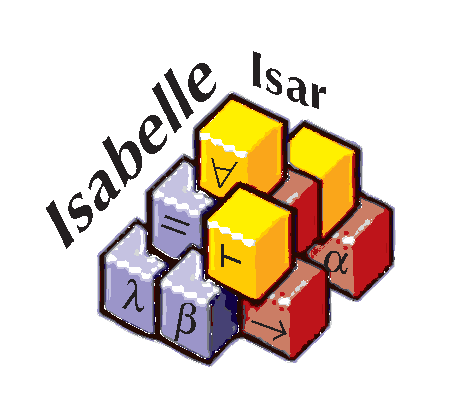
\includegraphics[scale=0.5]{isabelle_isar} \\[4ex] The Isabelle/Isar Reference Manual}
\author{\emph{Makarius Wenzel} \\[3ex]
  With Contributions by
  Clemens Ballarin,
  Stefan Berghofer, \\
  Jasmin Blanchette,
  Timothy Bourke,
  Lukas Bulwahn, \\
  Amine Chaieb,
  Lucas Dixon,
  Florian Haftmann, \\
  Brian Huffman,
  Lars Hupel,
  Gerwin Klein, \\
  Alexander Krauss,
  Ond\v{r}ej Kun\v{c}ar,
  Andreas Lochbihler, \\
  Tobias Nipkow,
  Lars Noschinski,
  David von Oheimb, \\
  Larry Paulson,
  Sebastian Skalberg,
  Christian Sternagel
}

\makeindex

\chardef\charbackquote=`\`
\newcommand{\backquote}{\mbox{\tt\charbackquote}}


\begin{document}

\maketitle 

\pagenumbering{roman}
{\def\isamarkupchapter#1{\chapter*{#1}}%
\begin{isabellebody}%
\def\isabellecontext{Preface}%
%
\isadelimtheory
%
\endisadelimtheory
%
\isatagtheory
\isacommand{theory}\isamarkupfalse%
\ Preface\isanewline
\isakeyword{imports}\ Base\ Main\isanewline
\isakeyword{begin}%
\endisatagtheory
{\isafoldtheory}%
%
\isadelimtheory
%
\endisadelimtheory
%
\isamarkupchapter{Preface%
}
\isamarkuptrue%
%
\begin{isamarkuptext}%
The \emph{Isabelle} system essentially provides a generic
  infrastructure for building deductive systems (programmed in
  Standard ML), with a special focus on interactive theorem proving in
  higher-order logics.  Many years ago, even end-users would refer to
  certain ML functions (goal commands, tactics, tacticals etc.) to
  pursue their everyday theorem proving tasks.
  
  In contrast \emph{Isar} provides an interpreted language environment
  of its own, which has been specifically tailored for the needs of
  theory and proof development.  Compared to raw ML, the Isabelle/Isar
  top-level provides a more robust and comfortable development
  platform, with proper support for theory development graphs, managed
  transactions with unlimited undo etc.  The Isabelle/Isar version of
  the \emph{Proof~General} user interface
  \cite{proofgeneral,Aspinall:TACAS:2000} provides a decent front-end
  for interactive theory and proof development in this advanced
  theorem proving environment, even though it is somewhat biased
  towards old-style proof scripts.

  \medskip Apart from the technical advances over bare-bones ML
  programming, the main purpose of the Isar language is to provide a
  conceptually different view on machine-checked proofs
  \cite{Wenzel:1999:TPHOL,Wenzel-PhD}.  \emph{Isar} stands for
  \emph{Intelligible semi-automated reasoning}.  Drawing from both the
  traditions of informal mathematical proof texts and high-level
  programming languages, Isar offers a versatile environment for
  structured formal proof documents.  Thus properly written Isar
  proofs become accessible to a broader audience than unstructured
  tactic scripts (which typically only provide operational information
  for the machine).  Writing human-readable proof texts certainly
  requires some additional efforts by the writer to achieve a good
  presentation, both of formal and informal parts of the text.  On the
  other hand, human-readable formal texts gain some value in their own
  right, independently of the mechanic proof-checking process.

  Despite its grand design of structured proof texts, Isar is able to
  assimilate the old tactical style as an ``improper'' sub-language.
  This provides an easy upgrade path for existing tactic scripts, as
  well as some means for interactive experimentation and debugging of
  structured proofs.  Isabelle/Isar supports a broad range of proof
  styles, both readable and unreadable ones.

  \medskip The generic Isabelle/Isar framework (see
  \chref{ch:isar-framework}) works reasonably well for any Isabelle
  object-logic that conforms to the natural deduction view of the
  Isabelle/Pure framework.  Specific language elements introduced by
  Isabelle/HOL are described in \chref{ch:hol}.  Although the main
  language elements are already provided by the Isabelle/Pure
  framework, examples given in the generic parts will usually refer to
  Isabelle/HOL.

  \medskip Isar commands may be either \emph{proper} document
  constructors, or \emph{improper commands}.  Some proof methods and
  attributes introduced later are classified as improper as well.
  Improper Isar language elements, which are marked by ``\isa{{\isaliteral{22}{\isachardoublequote}}\isaliteral{5C3C5E7375703E}{}\isactrlsup {\isaliteral{2A}{\isacharasterisk}}{\isaliteral{22}{\isachardoublequote}}}'' in the subsequent chapters; they are often helpful
  when developing proof documents, but their use is discouraged for
  the final human-readable outcome.  Typical examples are diagnostic
  commands that print terms or theorems according to the current
  context; other commands emulate old-style tactical theorem proving.%
\end{isamarkuptext}%
\isamarkuptrue%
%
\isadelimtheory
%
\endisadelimtheory
%
\isatagtheory
\isacommand{end}\isamarkupfalse%
%
\endisatagtheory
{\isafoldtheory}%
%
\isadelimtheory
%
\endisadelimtheory
\isanewline
\end{isabellebody}%
%%% Local Variables:
%%% mode: latex
%%% TeX-master: "root"
%%% End:
}
\tableofcontents
\clearfirst

\part{Basic Concepts}
%
\begin{isabellebody}%
\def\isabellecontext{Synopsis}%
%
\isadelimtheory
%
\endisadelimtheory
%
\isatagtheory
\isacommand{theory}\isamarkupfalse%
\ Synopsis\isanewline
\isakeyword{imports}\ Base\ Main\isanewline
\isakeyword{begin}%
\endisatagtheory
{\isafoldtheory}%
%
\isadelimtheory
%
\endisadelimtheory
%
\isamarkupchapter{Synopsis%
}
\isamarkuptrue%
%
\isamarkupsection{Notepad%
}
\isamarkuptrue%
%
\begin{isamarkuptext}%
An Isar proof body serves as mathematical notepad to compose logical
  content, consisting of facts, terms, types.%
\end{isamarkuptext}%
\isamarkuptrue%
%
\isamarkupsubsection{Facts%
}
\isamarkuptrue%
%
\begin{isamarkuptext}%
A fact is a simultaneous list of theorems.%
\end{isamarkuptext}%
\isamarkuptrue%
%
\isamarkupsubsubsection{Producing facts%
}
\isamarkuptrue%
\isacommand{notepad}\isamarkupfalse%
\isanewline
\isakeyword{begin}%
\isadelimproof
%
\endisadelimproof
%
\isatagproof
%
\begin{isamarkuptxt}%
Via assumption (``lambda''):%
\end{isamarkuptxt}%
\isamarkuptrue%
\ \ \isacommand{assume}\isamarkupfalse%
\ a{\isaliteral{3A}{\isacharcolon}}\ A%
\begin{isamarkuptxt}%
Via proof (``let''):%
\end{isamarkuptxt}%
\isamarkuptrue%
\ \ \isacommand{have}\isamarkupfalse%
\ b{\isaliteral{3A}{\isacharcolon}}\ B\ \isacommand{sorry}\isamarkupfalse%
%
\begin{isamarkuptxt}%
Via abbreviation (``let''):%
\end{isamarkuptxt}%
\isamarkuptrue%
\ \ \isacommand{note}\isamarkupfalse%
\ c\ {\isaliteral{3D}{\isacharequal}}\ a\ b%
\endisatagproof
{\isafoldproof}%
%
\isadelimproof
%
\endisadelimproof
\isanewline
\isanewline
\isacommand{end}\isamarkupfalse%
%
\isamarkupsubsubsection{Referencing facts%
}
\isamarkuptrue%
\isacommand{notepad}\isamarkupfalse%
\isanewline
\isakeyword{begin}%
\isadelimproof
%
\endisadelimproof
%
\isatagproof
%
\begin{isamarkuptxt}%
Via explicit name:%
\end{isamarkuptxt}%
\isamarkuptrue%
\ \ \isacommand{assume}\isamarkupfalse%
\ a{\isaliteral{3A}{\isacharcolon}}\ A\isanewline
\ \ \isacommand{note}\isamarkupfalse%
\ a%
\begin{isamarkuptxt}%
Via implicit name:%
\end{isamarkuptxt}%
\isamarkuptrue%
\ \ \isacommand{assume}\isamarkupfalse%
\ A\isanewline
\ \ \isacommand{note}\isamarkupfalse%
\ this%
\begin{isamarkuptxt}%
Via literal proposition (unification with results from the proof text):%
\end{isamarkuptxt}%
\isamarkuptrue%
\ \ \isacommand{assume}\isamarkupfalse%
\ A\isanewline
\ \ \isacommand{note}\isamarkupfalse%
\ {\isaliteral{60}{\isacharbackquoteopen}}A{\isaliteral{60}{\isacharbackquoteclose}}\isanewline
\isanewline
\ \ \isacommand{assume}\isamarkupfalse%
\ {\isaliteral{22}{\isachardoublequoteopen}}{\isaliteral{5C3C416E643E}{\isasymAnd}}x{\isaliteral{2E}{\isachardot}}\ B\ x{\isaliteral{22}{\isachardoublequoteclose}}\isanewline
\ \ \isacommand{note}\isamarkupfalse%
\ {\isaliteral{60}{\isacharbackquoteopen}}B\ a{\isaliteral{60}{\isacharbackquoteclose}}\isanewline
\ \ \isacommand{note}\isamarkupfalse%
\ {\isaliteral{60}{\isacharbackquoteopen}}B\ b{\isaliteral{60}{\isacharbackquoteclose}}%
\endisatagproof
{\isafoldproof}%
%
\isadelimproof
%
\endisadelimproof
\isanewline
\isacommand{end}\isamarkupfalse%
%
\isamarkupsubsubsection{Manipulating facts%
}
\isamarkuptrue%
\isacommand{notepad}\isamarkupfalse%
\isanewline
\isakeyword{begin}%
\isadelimproof
%
\endisadelimproof
%
\isatagproof
%
\begin{isamarkuptxt}%
Instantiation:%
\end{isamarkuptxt}%
\isamarkuptrue%
\ \ \isacommand{assume}\isamarkupfalse%
\ a{\isaliteral{3A}{\isacharcolon}}\ {\isaliteral{22}{\isachardoublequoteopen}}{\isaliteral{5C3C416E643E}{\isasymAnd}}x{\isaliteral{2E}{\isachardot}}\ B\ x{\isaliteral{22}{\isachardoublequoteclose}}\isanewline
\ \ \isacommand{note}\isamarkupfalse%
\ a\isanewline
\ \ \isacommand{note}\isamarkupfalse%
\ a\ {\isaliteral{5B}{\isacharbrackleft}}of\ b{\isaliteral{5D}{\isacharbrackright}}\isanewline
\ \ \isacommand{note}\isamarkupfalse%
\ a\ {\isaliteral{5B}{\isacharbrackleft}}\isakeyword{where}\ x\ {\isaliteral{3D}{\isacharequal}}\ b{\isaliteral{5D}{\isacharbrackright}}%
\begin{isamarkuptxt}%
Backchaining:%
\end{isamarkuptxt}%
\isamarkuptrue%
\ \ \isacommand{assume}\isamarkupfalse%
\ {\isadigit{1}}{\isaliteral{3A}{\isacharcolon}}\ A\isanewline
\ \ \isacommand{assume}\isamarkupfalse%
\ {\isadigit{2}}{\isaliteral{3A}{\isacharcolon}}\ {\isaliteral{22}{\isachardoublequoteopen}}A\ {\isaliteral{5C3C4C6F6E6772696768746172726F773E}{\isasymLongrightarrow}}\ C{\isaliteral{22}{\isachardoublequoteclose}}\isanewline
\ \ \isacommand{note}\isamarkupfalse%
\ {\isadigit{2}}\ {\isaliteral{5B}{\isacharbrackleft}}OF\ {\isadigit{1}}{\isaliteral{5D}{\isacharbrackright}}\isanewline
\ \ \isacommand{note}\isamarkupfalse%
\ {\isadigit{1}}\ {\isaliteral{5B}{\isacharbrackleft}}THEN\ {\isadigit{2}}{\isaliteral{5D}{\isacharbrackright}}%
\begin{isamarkuptxt}%
Symmetric results:%
\end{isamarkuptxt}%
\isamarkuptrue%
\ \ \isacommand{assume}\isamarkupfalse%
\ {\isaliteral{22}{\isachardoublequoteopen}}x\ {\isaliteral{3D}{\isacharequal}}\ y{\isaliteral{22}{\isachardoublequoteclose}}\isanewline
\ \ \isacommand{note}\isamarkupfalse%
\ this\ {\isaliteral{5B}{\isacharbrackleft}}symmetric{\isaliteral{5D}{\isacharbrackright}}\isanewline
\isanewline
\ \ \isacommand{assume}\isamarkupfalse%
\ {\isaliteral{22}{\isachardoublequoteopen}}x\ {\isaliteral{5C3C6E6F7465713E}{\isasymnoteq}}\ y{\isaliteral{22}{\isachardoublequoteclose}}\isanewline
\ \ \isacommand{note}\isamarkupfalse%
\ this\ {\isaliteral{5B}{\isacharbrackleft}}symmetric{\isaliteral{5D}{\isacharbrackright}}%
\begin{isamarkuptxt}%
Adhoc-simplication (take care!):%
\end{isamarkuptxt}%
\isamarkuptrue%
\ \ \isacommand{assume}\isamarkupfalse%
\ {\isaliteral{22}{\isachardoublequoteopen}}P\ {\isaliteral{28}{\isacharparenleft}}{\isaliteral{5B}{\isacharbrackleft}}{\isaliteral{5D}{\isacharbrackright}}\ {\isaliteral{40}{\isacharat}}\ xs{\isaliteral{29}{\isacharparenright}}{\isaliteral{22}{\isachardoublequoteclose}}\isanewline
\ \ \isacommand{note}\isamarkupfalse%
\ this\ {\isaliteral{5B}{\isacharbrackleft}}simplified{\isaliteral{5D}{\isacharbrackright}}%
\endisatagproof
{\isafoldproof}%
%
\isadelimproof
%
\endisadelimproof
\isanewline
\isacommand{end}\isamarkupfalse%
%
\isamarkupsubsubsection{Projections%
}
\isamarkuptrue%
%
\begin{isamarkuptext}%
Isar facts consist of multiple theorems.  There is notation to project
  interval ranges.%
\end{isamarkuptext}%
\isamarkuptrue%
\isacommand{notepad}\isamarkupfalse%
\isanewline
\isakeyword{begin}\isanewline
%
\isadelimproof
\ \ %
\endisadelimproof
%
\isatagproof
\isacommand{assume}\isamarkupfalse%
\ stuff{\isaliteral{3A}{\isacharcolon}}\ A\ B\ C\ D\isanewline
\ \ \isacommand{note}\isamarkupfalse%
\ stuff{\isaliteral{28}{\isacharparenleft}}{\isadigit{1}}{\isaliteral{29}{\isacharparenright}}\isanewline
\ \ \isacommand{note}\isamarkupfalse%
\ stuff{\isaliteral{28}{\isacharparenleft}}{\isadigit{2}}{\isaliteral{2D}{\isacharminus}}{\isadigit{3}}{\isaliteral{29}{\isacharparenright}}\isanewline
\ \ \isacommand{note}\isamarkupfalse%
\ stuff{\isaliteral{28}{\isacharparenleft}}{\isadigit{2}}{\isaliteral{2D}{\isacharminus}}{\isaliteral{29}{\isacharparenright}}%
\endisatagproof
{\isafoldproof}%
%
\isadelimproof
\isanewline
%
\endisadelimproof
\isacommand{end}\isamarkupfalse%
%
\isamarkupsubsubsection{Naming conventions%
}
\isamarkuptrue%
%
\begin{isamarkuptext}%
\begin{itemize}

  \item Lower-case identifiers are usually preferred.

  \item Facts can be named after the main term within the proposition.

  \item Facts should \emph{not} be named after the command that
  introduced them (\hyperlink{command.assume}{\mbox{\isa{\isacommand{assume}}}}, \hyperlink{command.have}{\mbox{\isa{\isacommand{have}}}}).  This is
  misleading and hard to maintain.

  \item Natural numbers can be used as ``meaningless'' names (more
  appropriate than \isa{{\isaliteral{22}{\isachardoublequote}}a{\isadigit{1}}{\isaliteral{22}{\isachardoublequote}}}, \isa{{\isaliteral{22}{\isachardoublequote}}a{\isadigit{2}}{\isaliteral{22}{\isachardoublequote}}} etc.)

  \item Symbolic identifiers are supported (e.g. \isa{{\isaliteral{22}{\isachardoublequote}}{\isaliteral{2A}{\isacharasterisk}}{\isaliteral{22}{\isachardoublequote}}}, \isa{{\isaliteral{22}{\isachardoublequote}}{\isaliteral{2A}{\isacharasterisk}}{\isaliteral{2A}{\isacharasterisk}}{\isaliteral{22}{\isachardoublequote}}}, \isa{{\isaliteral{22}{\isachardoublequote}}{\isaliteral{2A}{\isacharasterisk}}{\isaliteral{2A}{\isacharasterisk}}{\isaliteral{2A}{\isacharasterisk}}{\isaliteral{22}{\isachardoublequote}}}).

  \end{itemize}%
\end{isamarkuptext}%
\isamarkuptrue%
%
\isamarkupsubsection{Block structure%
}
\isamarkuptrue%
%
\begin{isamarkuptext}%
The formal notepad is block structured.  The fact produced by the last
  entry of a block is exported into the outer context.%
\end{isamarkuptext}%
\isamarkuptrue%
\isacommand{notepad}\isamarkupfalse%
\isanewline
\isakeyword{begin}\isanewline
%
\isadelimproof
\ \ %
\endisadelimproof
%
\isatagproof
\isacommand{{\isaliteral{7B}{\isacharbraceleft}}}\isamarkupfalse%
\isanewline
\ \ \ \ \isacommand{have}\isamarkupfalse%
\ a{\isaliteral{3A}{\isacharcolon}}\ A\ \isacommand{sorry}\isamarkupfalse%
\isanewline
\ \ \ \ \isacommand{have}\isamarkupfalse%
\ b{\isaliteral{3A}{\isacharcolon}}\ B\ \isacommand{sorry}\isamarkupfalse%
\isanewline
\ \ \ \ \isacommand{note}\isamarkupfalse%
\ a\ b\isanewline
\ \ \isacommand{{\isaliteral{7D}{\isacharbraceright}}}\isamarkupfalse%
\isanewline
\ \ \isacommand{note}\isamarkupfalse%
\ this\isanewline
\ \ \isacommand{note}\isamarkupfalse%
\ {\isaliteral{60}{\isacharbackquoteopen}}A{\isaliteral{60}{\isacharbackquoteclose}}\isanewline
\ \ \isacommand{note}\isamarkupfalse%
\ {\isaliteral{60}{\isacharbackquoteopen}}B{\isaliteral{60}{\isacharbackquoteclose}}%
\endisatagproof
{\isafoldproof}%
%
\isadelimproof
\isanewline
%
\endisadelimproof
\isacommand{end}\isamarkupfalse%
%
\begin{isamarkuptext}%
Explicit blocks as well as implicit blocks of nested goal
  statements (e.g.\ \hyperlink{command.have}{\mbox{\isa{\isacommand{have}}}}) automatically introduce one extra
  pair of parentheses in reserve.  The \hyperlink{command.next}{\mbox{\isa{\isacommand{next}}}} command allows
  to ``jump'' these sub-blocks.%
\end{isamarkuptext}%
\isamarkuptrue%
\isacommand{notepad}\isamarkupfalse%
\isanewline
\isakeyword{begin}\isanewline
%
\isadelimproof
\isanewline
\ \ %
\endisadelimproof
%
\isatagproof
\isacommand{{\isaliteral{7B}{\isacharbraceleft}}}\isamarkupfalse%
\isanewline
\ \ \ \ \isacommand{have}\isamarkupfalse%
\ a{\isaliteral{3A}{\isacharcolon}}\ A\ \isacommand{sorry}\isamarkupfalse%
\isanewline
\ \ \isacommand{next}\isamarkupfalse%
\isanewline
\ \ \ \ \isacommand{have}\isamarkupfalse%
\ b{\isaliteral{3A}{\isacharcolon}}\ B\isanewline
\ \ \ \ \isacommand{proof}\isamarkupfalse%
\ {\isaliteral{2D}{\isacharminus}}\isanewline
\ \ \ \ \ \ \isacommand{show}\isamarkupfalse%
\ B\ \isacommand{sorry}\isamarkupfalse%
\isanewline
\ \ \ \ \isacommand{next}\isamarkupfalse%
\isanewline
\ \ \ \ \ \ \isacommand{have}\isamarkupfalse%
\ c{\isaliteral{3A}{\isacharcolon}}\ C\ \isacommand{sorry}\isamarkupfalse%
\isanewline
\ \ \ \ \isacommand{next}\isamarkupfalse%
\isanewline
\ \ \ \ \ \ \isacommand{have}\isamarkupfalse%
\ d{\isaliteral{3A}{\isacharcolon}}\ D\ \isacommand{sorry}\isamarkupfalse%
\isanewline
\ \ \ \ \isacommand{qed}\isamarkupfalse%
\isanewline
\ \ \isacommand{{\isaliteral{7D}{\isacharbraceright}}}\isamarkupfalse%
%
\begin{isamarkuptxt}%
Alternative version with explicit parentheses everywhere:%
\end{isamarkuptxt}%
\isamarkuptrue%
\ \ \isacommand{{\isaliteral{7B}{\isacharbraceleft}}}\isamarkupfalse%
\isanewline
\ \ \ \ \isacommand{{\isaliteral{7B}{\isacharbraceleft}}}\isamarkupfalse%
\isanewline
\ \ \ \ \ \ \isacommand{have}\isamarkupfalse%
\ a{\isaliteral{3A}{\isacharcolon}}\ A\ \isacommand{sorry}\isamarkupfalse%
\isanewline
\ \ \ \ \isacommand{{\isaliteral{7D}{\isacharbraceright}}}\isamarkupfalse%
\isanewline
\ \ \ \ \isacommand{{\isaliteral{7B}{\isacharbraceleft}}}\isamarkupfalse%
\isanewline
\ \ \ \ \ \ \isacommand{have}\isamarkupfalse%
\ b{\isaliteral{3A}{\isacharcolon}}\ B\isanewline
\ \ \ \ \ \ \isacommand{proof}\isamarkupfalse%
\ {\isaliteral{2D}{\isacharminus}}\isanewline
\ \ \ \ \ \ \ \ \isacommand{{\isaliteral{7B}{\isacharbraceleft}}}\isamarkupfalse%
\isanewline
\ \ \ \ \ \ \ \ \ \ \isacommand{show}\isamarkupfalse%
\ B\ \isacommand{sorry}\isamarkupfalse%
\isanewline
\ \ \ \ \ \ \ \ \isacommand{{\isaliteral{7D}{\isacharbraceright}}}\isamarkupfalse%
\isanewline
\ \ \ \ \ \ \ \ \isacommand{{\isaliteral{7B}{\isacharbraceleft}}}\isamarkupfalse%
\isanewline
\ \ \ \ \ \ \ \ \ \ \isacommand{have}\isamarkupfalse%
\ c{\isaliteral{3A}{\isacharcolon}}\ C\ \isacommand{sorry}\isamarkupfalse%
\isanewline
\ \ \ \ \ \ \ \ \isacommand{{\isaliteral{7D}{\isacharbraceright}}}\isamarkupfalse%
\isanewline
\ \ \ \ \ \ \ \ \isacommand{{\isaliteral{7B}{\isacharbraceleft}}}\isamarkupfalse%
\isanewline
\ \ \ \ \ \ \ \ \ \ \isacommand{have}\isamarkupfalse%
\ d{\isaliteral{3A}{\isacharcolon}}\ D\ \isacommand{sorry}\isamarkupfalse%
\isanewline
\ \ \ \ \ \ \ \ \isacommand{{\isaliteral{7D}{\isacharbraceright}}}\isamarkupfalse%
\isanewline
\ \ \ \ \ \ \isacommand{qed}\isamarkupfalse%
\isanewline
\ \ \ \ \isacommand{{\isaliteral{7D}{\isacharbraceright}}}\isamarkupfalse%
\isanewline
\ \ \isacommand{{\isaliteral{7D}{\isacharbraceright}}}\isamarkupfalse%
%
\endisatagproof
{\isafoldproof}%
%
\isadelimproof
\isanewline
%
\endisadelimproof
\isanewline
\isacommand{end}\isamarkupfalse%
%
\isamarkupsubsection{Terms and Types%
}
\isamarkuptrue%
\isacommand{notepad}\isamarkupfalse%
\isanewline
\isakeyword{begin}%
\isadelimproof
%
\endisadelimproof
%
\isatagproof
%
\begin{isamarkuptxt}%
Locally fixed entities:%
\end{isamarkuptxt}%
\isamarkuptrue%
\ \ \isacommand{fix}\isamarkupfalse%
\ x\ \ \ %
\isamarkupcmt{local constant, without any type information yet%
}
\isanewline
\ \ \isacommand{fix}\isamarkupfalse%
\ x\ {\isaliteral{3A}{\isacharcolon}}{\isaliteral{3A}{\isacharcolon}}\ {\isaliteral{27}{\isacharprime}}a\ \ %
\isamarkupcmt{variant with explicit type-constraint for subsequent use%
}
\isanewline
\isanewline
\ \ \isacommand{fix}\isamarkupfalse%
\ a\ b\isanewline
\ \ \isacommand{assume}\isamarkupfalse%
\ {\isaliteral{22}{\isachardoublequoteopen}}a\ {\isaliteral{3D}{\isacharequal}}\ b{\isaliteral{22}{\isachardoublequoteclose}}\ \ %
\isamarkupcmt{type assignment at first occurrence in concrete term%
}
%
\begin{isamarkuptxt}%
Definitions (non-polymorphic):%
\end{isamarkuptxt}%
\isamarkuptrue%
\ \ \isacommand{def}\isamarkupfalse%
\ x\ {\isaliteral{5C3C65717569763E}{\isasymequiv}}\ {\isaliteral{22}{\isachardoublequoteopen}}t{\isaliteral{3A}{\isacharcolon}}{\isaliteral{3A}{\isacharcolon}}{\isaliteral{27}{\isacharprime}}a{\isaliteral{22}{\isachardoublequoteclose}}%
\begin{isamarkuptxt}%
Abbreviations (polymorphic):%
\end{isamarkuptxt}%
\isamarkuptrue%
\ \ \isacommand{let}\isamarkupfalse%
\ {\isaliteral{3F}{\isacharquery}}f\ {\isaliteral{3D}{\isacharequal}}\ {\isaliteral{22}{\isachardoublequoteopen}}{\isaliteral{5C3C6C616D6264613E}{\isasymlambda}}x{\isaliteral{2E}{\isachardot}}\ x{\isaliteral{22}{\isachardoublequoteclose}}%
\endisatagproof
{\isafoldproof}%
%
\isadelimproof
%
\endisadelimproof
\isanewline
\ \ \isacommand{term}\isamarkupfalse%
\ {\isaliteral{22}{\isachardoublequoteopen}}{\isaliteral{3F}{\isacharquery}}f\ {\isaliteral{3F}{\isacharquery}}f{\isaliteral{22}{\isachardoublequoteclose}}%
\isadelimproof
%
\endisadelimproof
%
\isatagproof
%
\begin{isamarkuptxt}%
Notation:%
\end{isamarkuptxt}%
\isamarkuptrue%
\ \ \isacommand{write}\isamarkupfalse%
\ x\ \ {\isaliteral{28}{\isacharparenleft}}{\isaliteral{22}{\isachardoublequoteopen}}{\isaliteral{2A}{\isacharasterisk}}{\isaliteral{2A}{\isacharasterisk}}{\isaliteral{2A}{\isacharasterisk}}{\isaliteral{22}{\isachardoublequoteclose}}{\isaliteral{29}{\isacharparenright}}%
\endisatagproof
{\isafoldproof}%
%
\isadelimproof
%
\endisadelimproof
\isanewline
\isacommand{end}\isamarkupfalse%
\isanewline
%
\isadelimtheory
\isanewline
%
\endisadelimtheory
%
\isatagtheory
\isacommand{end}\isamarkupfalse%
%
\endisatagtheory
{\isafoldtheory}%
%
\isadelimtheory
%
\endisadelimtheory
\end{isabellebody}%
%%% Local Variables:
%%% mode: latex
%%% TeX-master: "root"
%%% End:

%
\begin{isabellebody}%
\def\isabellecontext{Framework}%
%
\isadelimtheory
%
\endisadelimtheory
%
\isatagtheory
\isacommand{theory}\isamarkupfalse%
\ Framework\isanewline
\isakeyword{imports}\ Main\isanewline
\isakeyword{begin}%
\endisatagtheory
{\isafoldtheory}%
%
\isadelimtheory
%
\endisadelimtheory
%
\isamarkupchapter{The Isabelle/Isar Framework \label{ch:isar-framework}%
}
\isamarkuptrue%
%
\begin{isamarkuptext}%
Isabelle/Isar
  \cite{Wenzel:1999:TPHOL,Wenzel-PhD,Nipkow-TYPES02,Wenzel-Paulson:2006,Wenzel:2006:Festschrift}
  is intended as a generic framework for developing formal
  mathematical documents with full proof checking.  Definitions and
  proofs are organized as theories; an assembly of theory sources may
  be presented as a printed document; see also
  \chref{ch:document-prep}.

  The main objective of Isar is the design of a human-readable
  structured proof language, which is called the ``primary proof
  format'' in Isar terminology.  Such a primary proof language is
  somewhere in the middle between the extremes of primitive proof
  objects and actual natural language.  In this respect, Isar is a bit
  more formalistic than Mizar
  \cite{Trybulec:1993:MizarFeatures,Rudnicki:1992:MizarOverview,Wiedijk:1999:Mizar},
  using logical symbols for certain reasoning schemes where Mizar
  would prefer English words; see \cite{Wenzel-Wiedijk:2002} for
  further comparisons of these systems.

  So Isar challenges the traditional way of recording informal proofs
  in mathematical prose, as well as the common tendency to see fully
  formal proofs directly as objects of some logical calculus (e.g.\
  \isa{{\isachardoublequote}{\isasymlambda}{\isachardoublequote}}-terms in a version of type theory).  In fact, Isar is
  better understood as an interpreter of a simple block-structured
  language for describing data flow of local facts and goals,
  interspersed with occasional invocations of proof methods.
  Everything is reduced to logical inferences internally, but these
  steps are somewhat marginal compared to the overall bookkeeping of
  the interpretation process.  Thanks to careful design of the syntax
  and semantics of Isar language elements, a formal record of Isar
  instructions may later appear as an intelligible text to the
  attentive reader.

  The Isar proof language has emerged from careful analysis of some
  inherent virtues of the existing logical framework of Isabelle/Pure
  \cite{paulson-found,paulson700}, notably composition of higher-order
  natural deduction rules, which is a generalization of Gentzen's
  original calculus \cite{Gentzen:1935}.  The approach of generic
  inference systems in Pure is continued by Isar towards actual proof
  texts.

  Concrete applications require another intermediate layer: an
  object-logic.  Isabelle/HOL \cite{isa-tutorial} (simply-typed
  set-theory) is being used most of the time; Isabelle/ZF
  \cite{isabelle-ZF} is less extensively developed, although it would
  probably fit better for classical mathematics.%
\end{isamarkuptext}%
\isamarkuptrue%
%
\isadelimtheory
%
\endisadelimtheory
%
\isatagtheory
\isacommand{end}\isamarkupfalse%
%
\endisatagtheory
{\isafoldtheory}%
%
\isadelimtheory
%
\endisadelimtheory
\isanewline
\end{isabellebody}%
%%% Local Variables:
%%% mode: latex
%%% TeX-master: "root"
%%% End:

%
\begin{isabellebody}%
\def\isabellecontext{First{\isacharunderscore}Order{\isacharunderscore}Logic}%
%
\isamarkupheader{Example: First-Order Logic%
}
\isamarkuptrue%
%
\isadelimvisible
%
\endisadelimvisible
%
\isatagvisible
\isacommand{theory}\isamarkupfalse%
\ First{\isacharunderscore}Order{\isacharunderscore}Logic\isanewline
\isakeyword{imports}\ Pure\isanewline
\isakeyword{begin}%
\endisatagvisible
{\isafoldvisible}%
%
\isadelimvisible
%
\endisadelimvisible
%
\begin{isamarkuptext}%
\noindent In order to commence a new object-logic within
  Isabelle/Pure we introduce abstract syntactic categories \isa{{\isachardoublequote}i{\isachardoublequote}}
  for individuals and \isa{{\isachardoublequote}o{\isachardoublequote}} for object-propositions.  The latter
  is embedded into the language of Pure propositions by means of a
  separate judgment.%
\end{isamarkuptext}%
\isamarkuptrue%
\isacommand{typedecl}\isamarkupfalse%
\ i\isanewline
\isacommand{typedecl}\isamarkupfalse%
\ o\isanewline
\isanewline
\isacommand{judgment}\isamarkupfalse%
\isanewline
\ \ Trueprop\ {\isacharcolon}{\isacharcolon}\ {\isachardoublequoteopen}o\ {\isasymRightarrow}\ prop{\isachardoublequoteclose}\ \ \ \ {\isacharparenleft}{\isachardoublequoteopen}{\isacharunderscore}{\isachardoublequoteclose}\ {\isadigit{5}}{\isacharparenright}%
\begin{isamarkuptext}%
\noindent Note that the object-logic judgement is implicit in the
  syntax: writing \isa{A} produces \isa{{\isachardoublequote}Trueprop\ A{\isachardoublequote}} internally.
  From the Pure perspective this means ``\isa{A} is derivable in the
  object-logic''.%
\end{isamarkuptext}%
\isamarkuptrue%
%
\isamarkupsubsection{Equational reasoning \label{sec:framework-ex-equal}%
}
\isamarkuptrue%
%
\begin{isamarkuptext}%
Equality is axiomatized as a binary predicate on individuals, with
  reflexivity as introduction, and substitution as elimination
  principle.  Note that the latter is particularly convenient in a
  framework like Isabelle, because syntactic congruences are
  implicitly produced by unification of \isa{{\isachardoublequote}B\ x{\isachardoublequote}} against
  expressions containing occurrences of \isa{x}.%
\end{isamarkuptext}%
\isamarkuptrue%
\isacommand{axiomatization}\isamarkupfalse%
\isanewline
\ \ equal\ {\isacharcolon}{\isacharcolon}\ {\isachardoublequoteopen}i\ {\isasymRightarrow}\ i\ {\isasymRightarrow}\ o{\isachardoublequoteclose}\ \ {\isacharparenleft}\isakeyword{infix}\ {\isachardoublequoteopen}{\isacharequal}{\isachardoublequoteclose}\ {\isadigit{5}}{\isadigit{0}}{\isacharparenright}\isanewline
\isakeyword{where}\isanewline
\ \ refl\ {\isacharbrackleft}intro{\isacharbrackright}{\isacharcolon}\ {\isachardoublequoteopen}x\ {\isacharequal}\ x{\isachardoublequoteclose}\ \isakeyword{and}\isanewline
\ \ subst\ {\isacharbrackleft}elim{\isacharbrackright}{\isacharcolon}\ {\isachardoublequoteopen}x\ {\isacharequal}\ y\ {\isasymLongrightarrow}\ B\ x\ {\isasymLongrightarrow}\ B\ y{\isachardoublequoteclose}%
\begin{isamarkuptext}%
\noindent Substitution is very powerful, but also hard to control in
  full generality.  We derive some common symmetry~/ transitivity
  schemes of as particular consequences.%
\end{isamarkuptext}%
\isamarkuptrue%
\isacommand{theorem}\isamarkupfalse%
\ sym\ {\isacharbrackleft}sym{\isacharbrackright}{\isacharcolon}\isanewline
\ \ \isakeyword{assumes}\ {\isachardoublequoteopen}x\ {\isacharequal}\ y{\isachardoublequoteclose}\isanewline
\ \ \isakeyword{shows}\ {\isachardoublequoteopen}y\ {\isacharequal}\ x{\isachardoublequoteclose}\isanewline
%
\isadelimproof
%
\endisadelimproof
%
\isatagproof
\isacommand{proof}\isamarkupfalse%
\ {\isacharminus}\isanewline
\ \ \isacommand{have}\isamarkupfalse%
\ {\isachardoublequoteopen}x\ {\isacharequal}\ x{\isachardoublequoteclose}\ \isacommand{{\isachardot}{\isachardot}}\isamarkupfalse%
\isanewline
\ \ \isacommand{with}\isamarkupfalse%
\ {\isacharbackquoteopen}x\ {\isacharequal}\ y{\isacharbackquoteclose}\ \isacommand{show}\isamarkupfalse%
\ {\isachardoublequoteopen}y\ {\isacharequal}\ x{\isachardoublequoteclose}\ \isacommand{{\isachardot}{\isachardot}}\isamarkupfalse%
\isanewline
\isacommand{qed}\isamarkupfalse%
%
\endisatagproof
{\isafoldproof}%
%
\isadelimproof
\isanewline
%
\endisadelimproof
\isanewline
\isacommand{theorem}\isamarkupfalse%
\ forw{\isacharunderscore}subst\ {\isacharbrackleft}trans{\isacharbrackright}{\isacharcolon}\isanewline
\ \ \isakeyword{assumes}\ {\isachardoublequoteopen}y\ {\isacharequal}\ x{\isachardoublequoteclose}\ \isakeyword{and}\ {\isachardoublequoteopen}B\ x{\isachardoublequoteclose}\isanewline
\ \ \isakeyword{shows}\ {\isachardoublequoteopen}B\ y{\isachardoublequoteclose}\isanewline
%
\isadelimproof
%
\endisadelimproof
%
\isatagproof
\isacommand{proof}\isamarkupfalse%
\ {\isacharminus}\isanewline
\ \ \isacommand{from}\isamarkupfalse%
\ {\isacharbackquoteopen}y\ {\isacharequal}\ x{\isacharbackquoteclose}\ \isacommand{have}\isamarkupfalse%
\ {\isachardoublequoteopen}x\ {\isacharequal}\ y{\isachardoublequoteclose}\ \isacommand{{\isachardot}{\isachardot}}\isamarkupfalse%
\isanewline
\ \ \isacommand{from}\isamarkupfalse%
\ this\ \isakeyword{and}\ {\isacharbackquoteopen}B\ x{\isacharbackquoteclose}\ \isacommand{show}\isamarkupfalse%
\ {\isachardoublequoteopen}B\ y{\isachardoublequoteclose}\ \isacommand{{\isachardot}{\isachardot}}\isamarkupfalse%
\isanewline
\isacommand{qed}\isamarkupfalse%
%
\endisatagproof
{\isafoldproof}%
%
\isadelimproof
\isanewline
%
\endisadelimproof
\isanewline
\isacommand{theorem}\isamarkupfalse%
\ back{\isacharunderscore}subst\ {\isacharbrackleft}trans{\isacharbrackright}{\isacharcolon}\isanewline
\ \ \isakeyword{assumes}\ {\isachardoublequoteopen}B\ x{\isachardoublequoteclose}\ \isakeyword{and}\ {\isachardoublequoteopen}x\ {\isacharequal}\ y{\isachardoublequoteclose}\isanewline
\ \ \isakeyword{shows}\ {\isachardoublequoteopen}B\ y{\isachardoublequoteclose}\isanewline
%
\isadelimproof
%
\endisadelimproof
%
\isatagproof
\isacommand{proof}\isamarkupfalse%
\ {\isacharminus}\isanewline
\ \ \isacommand{from}\isamarkupfalse%
\ {\isacharbackquoteopen}x\ {\isacharequal}\ y{\isacharbackquoteclose}\ \isakeyword{and}\ {\isacharbackquoteopen}B\ x{\isacharbackquoteclose}\isanewline
\ \ \isacommand{show}\isamarkupfalse%
\ {\isachardoublequoteopen}B\ y{\isachardoublequoteclose}\ \isacommand{{\isachardot}{\isachardot}}\isamarkupfalse%
\isanewline
\isacommand{qed}\isamarkupfalse%
%
\endisatagproof
{\isafoldproof}%
%
\isadelimproof
\isanewline
%
\endisadelimproof
\isanewline
\isacommand{theorem}\isamarkupfalse%
\ trans\ {\isacharbrackleft}trans{\isacharbrackright}{\isacharcolon}\isanewline
\ \ \isakeyword{assumes}\ {\isachardoublequoteopen}x\ {\isacharequal}\ y{\isachardoublequoteclose}\ \isakeyword{and}\ {\isachardoublequoteopen}y\ {\isacharequal}\ z{\isachardoublequoteclose}\isanewline
\ \ \isakeyword{shows}\ {\isachardoublequoteopen}x\ {\isacharequal}\ z{\isachardoublequoteclose}\isanewline
%
\isadelimproof
%
\endisadelimproof
%
\isatagproof
\isacommand{proof}\isamarkupfalse%
\ {\isacharminus}\isanewline
\ \ \isacommand{from}\isamarkupfalse%
\ {\isacharbackquoteopen}y\ {\isacharequal}\ z{\isacharbackquoteclose}\ \isakeyword{and}\ {\isacharbackquoteopen}x\ {\isacharequal}\ y{\isacharbackquoteclose}\isanewline
\ \ \isacommand{show}\isamarkupfalse%
\ {\isachardoublequoteopen}x\ {\isacharequal}\ z{\isachardoublequoteclose}\ \isacommand{{\isachardot}{\isachardot}}\isamarkupfalse%
\isanewline
\isacommand{qed}\isamarkupfalse%
%
\endisatagproof
{\isafoldproof}%
%
\isadelimproof
%
\endisadelimproof
%
\isamarkupsubsection{Basic group theory%
}
\isamarkuptrue%
%
\begin{isamarkuptext}%
As an example for equational reasoning we consider some bits of
  group theory.  The subsequent locale definition postulates group
  operations and axioms; we also derive some consequences of this
  specification.%
\end{isamarkuptext}%
\isamarkuptrue%
\isacommand{locale}\isamarkupfalse%
\ group\ {\isacharequal}\isanewline
\ \ \isakeyword{fixes}\ prod\ {\isacharcolon}{\isacharcolon}\ {\isachardoublequoteopen}i\ {\isasymRightarrow}\ i\ {\isasymRightarrow}\ i{\isachardoublequoteclose}\ \ {\isacharparenleft}\isakeyword{infix}\ {\isachardoublequoteopen}{\isasymcirc}{\isachardoublequoteclose}\ {\isadigit{7}}{\isadigit{0}}{\isacharparenright}\isanewline
\ \ \ \ \isakeyword{and}\ inv\ {\isacharcolon}{\isacharcolon}\ {\isachardoublequoteopen}i\ {\isasymRightarrow}\ i{\isachardoublequoteclose}\ \ {\isacharparenleft}{\isachardoublequoteopen}{\isacharparenleft}{\isacharunderscore}{\isasyminverse}{\isacharparenright}{\isachardoublequoteclose}\ {\isacharbrackleft}{\isadigit{1}}{\isadigit{0}}{\isadigit{0}}{\isadigit{0}}{\isacharbrackright}\ {\isadigit{9}}{\isadigit{9}}{\isadigit{9}}{\isacharparenright}\isanewline
\ \ \ \ \isakeyword{and}\ unit\ {\isacharcolon}{\isacharcolon}\ i\ \ {\isacharparenleft}{\isachardoublequoteopen}{\isadigit{1}}{\isachardoublequoteclose}{\isacharparenright}\isanewline
\ \ \isakeyword{assumes}\ assoc{\isacharcolon}\ {\isachardoublequoteopen}{\isacharparenleft}x\ {\isasymcirc}\ y{\isacharparenright}\ {\isasymcirc}\ z\ {\isacharequal}\ x\ {\isasymcirc}\ {\isacharparenleft}y\ {\isasymcirc}\ z{\isacharparenright}{\isachardoublequoteclose}\isanewline
\ \ \ \ \isakeyword{and}\ left{\isacharunderscore}unit{\isacharcolon}\ \ {\isachardoublequoteopen}{\isadigit{1}}\ {\isasymcirc}\ x\ {\isacharequal}\ x{\isachardoublequoteclose}\isanewline
\ \ \ \ \isakeyword{and}\ left{\isacharunderscore}inv{\isacharcolon}\ {\isachardoublequoteopen}x{\isasyminverse}\ {\isasymcirc}\ x\ {\isacharequal}\ {\isadigit{1}}{\isachardoublequoteclose}\isanewline
\isakeyword{begin}\isanewline
\isanewline
\isacommand{theorem}\isamarkupfalse%
\ right{\isacharunderscore}inv{\isacharcolon}\ {\isachardoublequoteopen}x\ {\isasymcirc}\ x{\isasyminverse}\ {\isacharequal}\ {\isadigit{1}}{\isachardoublequoteclose}\isanewline
%
\isadelimproof
%
\endisadelimproof
%
\isatagproof
\isacommand{proof}\isamarkupfalse%
\ {\isacharminus}\isanewline
\ \ \isacommand{have}\isamarkupfalse%
\ {\isachardoublequoteopen}x\ {\isasymcirc}\ x{\isasyminverse}\ {\isacharequal}\ {\isadigit{1}}\ {\isasymcirc}\ {\isacharparenleft}x\ {\isasymcirc}\ x{\isasyminverse}{\isacharparenright}{\isachardoublequoteclose}\ \isacommand{by}\isamarkupfalse%
\ {\isacharparenleft}rule\ left{\isacharunderscore}unit\ {\isacharbrackleft}symmetric{\isacharbrackright}{\isacharparenright}\isanewline
\ \ \isacommand{also}\isamarkupfalse%
\ \isacommand{have}\isamarkupfalse%
\ {\isachardoublequoteopen}{\isasymdots}\ {\isacharequal}\ {\isacharparenleft}{\isadigit{1}}\ {\isasymcirc}\ x{\isacharparenright}\ {\isasymcirc}\ x{\isasyminverse}{\isachardoublequoteclose}\ \isacommand{by}\isamarkupfalse%
\ {\isacharparenleft}rule\ assoc\ {\isacharbrackleft}symmetric{\isacharbrackright}{\isacharparenright}\isanewline
\ \ \isacommand{also}\isamarkupfalse%
\ \isacommand{have}\isamarkupfalse%
\ {\isachardoublequoteopen}{\isadigit{1}}\ {\isacharequal}\ {\isacharparenleft}x{\isasyminverse}{\isacharparenright}{\isasyminverse}\ {\isasymcirc}\ x{\isasyminverse}{\isachardoublequoteclose}\ \isacommand{by}\isamarkupfalse%
\ {\isacharparenleft}rule\ left{\isacharunderscore}inv\ {\isacharbrackleft}symmetric{\isacharbrackright}{\isacharparenright}\isanewline
\ \ \isacommand{also}\isamarkupfalse%
\ \isacommand{have}\isamarkupfalse%
\ {\isachardoublequoteopen}{\isasymdots}\ {\isasymcirc}\ x\ {\isacharequal}\ {\isacharparenleft}x{\isasyminverse}{\isacharparenright}{\isasyminverse}\ {\isasymcirc}\ {\isacharparenleft}x{\isasyminverse}\ {\isasymcirc}\ x{\isacharparenright}{\isachardoublequoteclose}\ \isacommand{by}\isamarkupfalse%
\ {\isacharparenleft}rule\ assoc{\isacharparenright}\isanewline
\ \ \isacommand{also}\isamarkupfalse%
\ \isacommand{have}\isamarkupfalse%
\ {\isachardoublequoteopen}x{\isasyminverse}\ {\isasymcirc}\ x\ {\isacharequal}\ {\isadigit{1}}{\isachardoublequoteclose}\ \isacommand{by}\isamarkupfalse%
\ {\isacharparenleft}rule\ left{\isacharunderscore}inv{\isacharparenright}\isanewline
\ \ \isacommand{also}\isamarkupfalse%
\ \isacommand{have}\isamarkupfalse%
\ {\isachardoublequoteopen}{\isacharparenleft}{\isacharparenleft}x{\isasyminverse}{\isacharparenright}{\isasyminverse}\ {\isasymcirc}\ {\isasymdots}{\isacharparenright}\ {\isasymcirc}\ x{\isasyminverse}\ {\isacharequal}\ {\isacharparenleft}x{\isasyminverse}{\isacharparenright}{\isasyminverse}\ {\isasymcirc}\ {\isacharparenleft}{\isadigit{1}}\ {\isasymcirc}\ x{\isasyminverse}{\isacharparenright}{\isachardoublequoteclose}\ \isacommand{by}\isamarkupfalse%
\ {\isacharparenleft}rule\ assoc{\isacharparenright}\isanewline
\ \ \isacommand{also}\isamarkupfalse%
\ \isacommand{have}\isamarkupfalse%
\ {\isachardoublequoteopen}{\isadigit{1}}\ {\isasymcirc}\ x{\isasyminverse}\ {\isacharequal}\ x{\isasyminverse}{\isachardoublequoteclose}\ \isacommand{by}\isamarkupfalse%
\ {\isacharparenleft}rule\ left{\isacharunderscore}unit{\isacharparenright}\isanewline
\ \ \isacommand{also}\isamarkupfalse%
\ \isacommand{have}\isamarkupfalse%
\ {\isachardoublequoteopen}{\isacharparenleft}x{\isasyminverse}{\isacharparenright}{\isasyminverse}\ {\isasymcirc}\ {\isasymdots}\ {\isacharequal}\ {\isadigit{1}}{\isachardoublequoteclose}\ \isacommand{by}\isamarkupfalse%
\ {\isacharparenleft}rule\ left{\isacharunderscore}inv{\isacharparenright}\isanewline
\ \ \isacommand{finally}\isamarkupfalse%
\ \isacommand{show}\isamarkupfalse%
\ {\isachardoublequoteopen}x\ {\isasymcirc}\ x{\isasyminverse}\ {\isacharequal}\ {\isadigit{1}}{\isachardoublequoteclose}\ \isacommand{{\isachardot}}\isamarkupfalse%
\isanewline
\isacommand{qed}\isamarkupfalse%
%
\endisatagproof
{\isafoldproof}%
%
\isadelimproof
\isanewline
%
\endisadelimproof
\isanewline
\isacommand{theorem}\isamarkupfalse%
\ right{\isacharunderscore}unit{\isacharcolon}\ {\isachardoublequoteopen}x\ {\isasymcirc}\ {\isadigit{1}}\ {\isacharequal}\ x{\isachardoublequoteclose}\isanewline
%
\isadelimproof
%
\endisadelimproof
%
\isatagproof
\isacommand{proof}\isamarkupfalse%
\ {\isacharminus}\isanewline
\ \ \isacommand{have}\isamarkupfalse%
\ {\isachardoublequoteopen}{\isadigit{1}}\ {\isacharequal}\ x{\isasyminverse}\ {\isasymcirc}\ x{\isachardoublequoteclose}\ \isacommand{by}\isamarkupfalse%
\ {\isacharparenleft}rule\ left{\isacharunderscore}inv\ {\isacharbrackleft}symmetric{\isacharbrackright}{\isacharparenright}\isanewline
\ \ \isacommand{also}\isamarkupfalse%
\ \isacommand{have}\isamarkupfalse%
\ {\isachardoublequoteopen}x\ {\isasymcirc}\ {\isasymdots}\ {\isacharequal}\ {\isacharparenleft}x\ {\isasymcirc}\ x{\isasyminverse}{\isacharparenright}\ {\isasymcirc}\ x{\isachardoublequoteclose}\ \isacommand{by}\isamarkupfalse%
\ {\isacharparenleft}rule\ assoc\ {\isacharbrackleft}symmetric{\isacharbrackright}{\isacharparenright}\isanewline
\ \ \isacommand{also}\isamarkupfalse%
\ \isacommand{have}\isamarkupfalse%
\ {\isachardoublequoteopen}x\ {\isasymcirc}\ x{\isasyminverse}\ {\isacharequal}\ {\isadigit{1}}{\isachardoublequoteclose}\ \isacommand{by}\isamarkupfalse%
\ {\isacharparenleft}rule\ right{\isacharunderscore}inv{\isacharparenright}\isanewline
\ \ \isacommand{also}\isamarkupfalse%
\ \isacommand{have}\isamarkupfalse%
\ {\isachardoublequoteopen}{\isasymdots}\ {\isasymcirc}\ x\ {\isacharequal}\ x{\isachardoublequoteclose}\ \isacommand{by}\isamarkupfalse%
\ {\isacharparenleft}rule\ left{\isacharunderscore}unit{\isacharparenright}\isanewline
\ \ \isacommand{finally}\isamarkupfalse%
\ \isacommand{show}\isamarkupfalse%
\ {\isachardoublequoteopen}x\ {\isasymcirc}\ {\isadigit{1}}\ {\isacharequal}\ x{\isachardoublequoteclose}\ \isacommand{{\isachardot}}\isamarkupfalse%
\isanewline
\isacommand{qed}\isamarkupfalse%
%
\endisatagproof
{\isafoldproof}%
%
\isadelimproof
%
\endisadelimproof
%
\begin{isamarkuptext}%
\noindent Reasoning from basic axioms is often tedious.  Our proofs
  work by producing various instances of the given rules (potentially
  the symmetric form) using the pattern ``\hyperlink{command.have}{\mbox{\isa{\isacommand{have}}}}~\isa{eq}~\hyperlink{command.by}{\mbox{\isa{\isacommand{by}}}}~\isa{{\isachardoublequote}{\isacharparenleft}rule\ r{\isacharparenright}{\isachardoublequote}}'' and composing the chain of
  results via \hyperlink{command.also}{\mbox{\isa{\isacommand{also}}}}/\hyperlink{command.finally}{\mbox{\isa{\isacommand{finally}}}}.  These steps may
  involve any of the transitivity rules declared in
  \secref{sec:framework-ex-equal}, namely \isa{trans} in combining
  the first two results in \isa{right{\isacharunderscore}inv} and in the final steps of
  both proofs, \isa{forw{\isacharunderscore}subst} in the first combination of \isa{right{\isacharunderscore}unit}, and \isa{back{\isacharunderscore}subst} in all other calculational steps.

  Occasional substitutions in calculations are adequate, but should
  not be over-emphasized.  The other extreme is to compose a chain by
  plain transitivity only, with replacements occurring always in
  topmost position. For example:%
\end{isamarkuptext}%
\isamarkuptrue%
%
\isadelimproof
%
\endisadelimproof
%
\isatagproof
\ \ \isacommand{have}\isamarkupfalse%
\ {\isachardoublequoteopen}x\ {\isasymcirc}\ {\isadigit{1}}\ {\isacharequal}\ x\ {\isasymcirc}\ {\isacharparenleft}x{\isasyminverse}\ {\isasymcirc}\ x{\isacharparenright}{\isachardoublequoteclose}\ \isacommand{unfolding}\isamarkupfalse%
\ left{\isacharunderscore}inv\ \isacommand{{\isachardot}{\isachardot}}\isamarkupfalse%
\isanewline
\ \ \isacommand{also}\isamarkupfalse%
\ \isacommand{have}\isamarkupfalse%
\ {\isachardoublequoteopen}{\isasymdots}\ {\isacharequal}\ {\isacharparenleft}x\ {\isasymcirc}\ x{\isasyminverse}{\isacharparenright}\ {\isasymcirc}\ x{\isachardoublequoteclose}\ \isacommand{unfolding}\isamarkupfalse%
\ assoc\ \isacommand{{\isachardot}{\isachardot}}\isamarkupfalse%
\isanewline
\ \ \isacommand{also}\isamarkupfalse%
\ \isacommand{have}\isamarkupfalse%
\ {\isachardoublequoteopen}{\isasymdots}\ {\isacharequal}\ {\isadigit{1}}\ {\isasymcirc}\ x{\isachardoublequoteclose}\ \isacommand{unfolding}\isamarkupfalse%
\ right{\isacharunderscore}inv\ \isacommand{{\isachardot}{\isachardot}}\isamarkupfalse%
\isanewline
\ \ \isacommand{also}\isamarkupfalse%
\ \isacommand{have}\isamarkupfalse%
\ {\isachardoublequoteopen}{\isasymdots}\ {\isacharequal}\ x{\isachardoublequoteclose}\ \isacommand{unfolding}\isamarkupfalse%
\ left{\isacharunderscore}unit\ \isacommand{{\isachardot}{\isachardot}}\isamarkupfalse%
\isanewline
\ \ \isacommand{finally}\isamarkupfalse%
\ \isacommand{have}\isamarkupfalse%
\ {\isachardoublequoteopen}x\ {\isasymcirc}\ {\isadigit{1}}\ {\isacharequal}\ x{\isachardoublequoteclose}\ \isacommand{{\isachardot}}\isamarkupfalse%
%
\endisatagproof
{\isafoldproof}%
%
\isadelimproof
%
\endisadelimproof
%
\begin{isamarkuptext}%
\noindent Here we have re-used the built-in mechanism for unfolding
  definitions in order to normalize each equational problem.  A more
  realistic object-logic would include proper setup for the Simplifier
  (\secref{sec:simplifier}), the main automated tool for equational
  reasoning in Isabelle.  Then ``\hyperlink{command.unfolding}{\mbox{\isa{\isacommand{unfolding}}}}~\isa{left{\isacharunderscore}inv}~\hyperlink{command.ddot}{\mbox{\isa{\isacommand{{\isachardot}{\isachardot}}}}}'' would become ``\hyperlink{command.by}{\mbox{\isa{\isacommand{by}}}}~\isa{{\isachardoublequote}{\isacharparenleft}simp\ only{\isacharcolon}\ left{\isacharunderscore}inv{\isacharparenright}{\isachardoublequote}}'' etc.%
\end{isamarkuptext}%
\isamarkuptrue%
\isacommand{end}\isamarkupfalse%
%
\isamarkupsubsection{Propositional logic \label{sec:framework-ex-prop}%
}
\isamarkuptrue%
%
\begin{isamarkuptext}%
We axiomatize basic connectives of propositional logic: implication,
  disjunction, and conjunction.  The associated rules are modeled
  after Gentzen's system of Natural Deduction \cite{Gentzen:1935}.%
\end{isamarkuptext}%
\isamarkuptrue%
\isacommand{axiomatization}\isamarkupfalse%
\isanewline
\ \ imp\ {\isacharcolon}{\isacharcolon}\ {\isachardoublequoteopen}o\ {\isasymRightarrow}\ o\ {\isasymRightarrow}\ o{\isachardoublequoteclose}\ \ {\isacharparenleft}\isakeyword{infixr}\ {\isachardoublequoteopen}{\isasymlongrightarrow}{\isachardoublequoteclose}\ {\isadigit{2}}{\isadigit{5}}{\isacharparenright}\ \isakeyword{where}\isanewline
\ \ impI\ {\isacharbrackleft}intro{\isacharbrackright}{\isacharcolon}\ {\isachardoublequoteopen}{\isacharparenleft}A\ {\isasymLongrightarrow}\ B{\isacharparenright}\ {\isasymLongrightarrow}\ A\ {\isasymlongrightarrow}\ B{\isachardoublequoteclose}\ \isakeyword{and}\isanewline
\ \ impD\ {\isacharbrackleft}dest{\isacharbrackright}{\isacharcolon}\ {\isachardoublequoteopen}{\isacharparenleft}A\ {\isasymlongrightarrow}\ B{\isacharparenright}\ {\isasymLongrightarrow}\ A\ {\isasymLongrightarrow}\ B{\isachardoublequoteclose}\isanewline
\isanewline
\isacommand{axiomatization}\isamarkupfalse%
\isanewline
\ \ disj\ {\isacharcolon}{\isacharcolon}\ {\isachardoublequoteopen}o\ {\isasymRightarrow}\ o\ {\isasymRightarrow}\ o{\isachardoublequoteclose}\ \ {\isacharparenleft}\isakeyword{infixr}\ {\isachardoublequoteopen}{\isasymor}{\isachardoublequoteclose}\ {\isadigit{3}}{\isadigit{0}}{\isacharparenright}\ \isakeyword{where}\isanewline
\ \ disjI\isactrlisub {\isadigit{1}}\ {\isacharbrackleft}intro{\isacharbrackright}{\isacharcolon}\ {\isachardoublequoteopen}A\ {\isasymLongrightarrow}\ A\ {\isasymor}\ B{\isachardoublequoteclose}\ \isakeyword{and}\isanewline
\ \ disjI\isactrlisub {\isadigit{2}}\ {\isacharbrackleft}intro{\isacharbrackright}{\isacharcolon}\ {\isachardoublequoteopen}B\ {\isasymLongrightarrow}\ A\ {\isasymor}\ B{\isachardoublequoteclose}\ \isakeyword{and}\isanewline
\ \ disjE\ {\isacharbrackleft}elim{\isacharbrackright}{\isacharcolon}\ {\isachardoublequoteopen}A\ {\isasymor}\ B\ {\isasymLongrightarrow}\ {\isacharparenleft}A\ {\isasymLongrightarrow}\ C{\isacharparenright}\ {\isasymLongrightarrow}\ {\isacharparenleft}B\ {\isasymLongrightarrow}\ C{\isacharparenright}\ {\isasymLongrightarrow}\ C{\isachardoublequoteclose}\isanewline
\isanewline
\isacommand{axiomatization}\isamarkupfalse%
\isanewline
\ \ conj\ {\isacharcolon}{\isacharcolon}\ {\isachardoublequoteopen}o\ {\isasymRightarrow}\ o\ {\isasymRightarrow}\ o{\isachardoublequoteclose}\ \ {\isacharparenleft}\isakeyword{infixr}\ {\isachardoublequoteopen}{\isasymand}{\isachardoublequoteclose}\ {\isadigit{3}}{\isadigit{5}}{\isacharparenright}\ \isakeyword{where}\isanewline
\ \ conjI\ {\isacharbrackleft}intro{\isacharbrackright}{\isacharcolon}\ {\isachardoublequoteopen}A\ {\isasymLongrightarrow}\ B\ {\isasymLongrightarrow}\ A\ {\isasymand}\ B{\isachardoublequoteclose}\ \isakeyword{and}\isanewline
\ \ conjD\isactrlisub {\isadigit{1}}{\isacharcolon}\ {\isachardoublequoteopen}A\ {\isasymand}\ B\ {\isasymLongrightarrow}\ A{\isachardoublequoteclose}\ \isakeyword{and}\isanewline
\ \ conjD\isactrlisub {\isadigit{2}}{\isacharcolon}\ {\isachardoublequoteopen}A\ {\isasymand}\ B\ {\isasymLongrightarrow}\ B{\isachardoublequoteclose}%
\begin{isamarkuptext}%
\noindent The conjunctive destructions have the disadvantage that
  decomposing \isa{{\isachardoublequote}A\ {\isasymand}\ B{\isachardoublequote}} involves an immediate decision which
  component should be projected.  The more convenient simultaneous
  elimination \isa{{\isachardoublequote}A\ {\isasymand}\ B\ {\isasymLongrightarrow}\ {\isacharparenleft}A\ {\isasymLongrightarrow}\ B\ {\isasymLongrightarrow}\ C{\isacharparenright}\ {\isasymLongrightarrow}\ C{\isachardoublequote}} can be derived as
  follows:%
\end{isamarkuptext}%
\isamarkuptrue%
\isacommand{theorem}\isamarkupfalse%
\ conjE\ {\isacharbrackleft}elim{\isacharbrackright}{\isacharcolon}\isanewline
\ \ \isakeyword{assumes}\ {\isachardoublequoteopen}A\ {\isasymand}\ B{\isachardoublequoteclose}\isanewline
\ \ \isakeyword{obtains}\ A\ \isakeyword{and}\ B\isanewline
%
\isadelimproof
%
\endisadelimproof
%
\isatagproof
\isacommand{proof}\isamarkupfalse%
\isanewline
\ \ \isacommand{from}\isamarkupfalse%
\ {\isacharbackquoteopen}A\ {\isasymand}\ B{\isacharbackquoteclose}\ \isacommand{show}\isamarkupfalse%
\ A\ \isacommand{by}\isamarkupfalse%
\ {\isacharparenleft}rule\ conjD\isactrlisub {\isadigit{1}}{\isacharparenright}\isanewline
\ \ \isacommand{from}\isamarkupfalse%
\ {\isacharbackquoteopen}A\ {\isasymand}\ B{\isacharbackquoteclose}\ \isacommand{show}\isamarkupfalse%
\ B\ \isacommand{by}\isamarkupfalse%
\ {\isacharparenleft}rule\ conjD\isactrlisub {\isadigit{2}}{\isacharparenright}\isanewline
\isacommand{qed}\isamarkupfalse%
%
\endisatagproof
{\isafoldproof}%
%
\isadelimproof
%
\endisadelimproof
%
\begin{isamarkuptext}%
\noindent Here is an example of swapping conjuncts with a single
  intermediate elimination step:%
\end{isamarkuptext}%
\isamarkuptrue%
%
\isadelimproof
%
\endisadelimproof
%
\isatagproof
\ \ \isacommand{assume}\isamarkupfalse%
\ {\isachardoublequoteopen}A\ {\isasymand}\ B{\isachardoublequoteclose}\isanewline
\ \ \isacommand{then}\isamarkupfalse%
\ \isacommand{obtain}\isamarkupfalse%
\ B\ \isakeyword{and}\ A\ \isacommand{{\isachardot}{\isachardot}}\isamarkupfalse%
\isanewline
\ \ \isacommand{then}\isamarkupfalse%
\ \isacommand{have}\isamarkupfalse%
\ {\isachardoublequoteopen}B\ {\isasymand}\ A{\isachardoublequoteclose}\ \isacommand{{\isachardot}{\isachardot}}\isamarkupfalse%
%
\endisatagproof
{\isafoldproof}%
%
\isadelimproof
%
\endisadelimproof
%
\begin{isamarkuptext}%
\noindent Note that the analogous elimination rule for disjunction
  ``\isa{{\isachardoublequote}{\isasymASSUMES}\ A\ {\isasymor}\ B\ {\isasymOBTAINS}\ A\ {\isasymBBAR}\ B{\isachardoublequote}}'' coincides with
  the original axiomatization of \isa{disjE}.

  \medskip We continue propositional logic by introducing absurdity
  with its characteristic elimination.  Plain truth may then be
  defined as a proposition that is trivially true.%
\end{isamarkuptext}%
\isamarkuptrue%
\isacommand{axiomatization}\isamarkupfalse%
\isanewline
\ \ false\ {\isacharcolon}{\isacharcolon}\ o\ \ {\isacharparenleft}{\isachardoublequoteopen}{\isasymbottom}{\isachardoublequoteclose}{\isacharparenright}\ \isakeyword{where}\isanewline
\ \ falseE\ {\isacharbrackleft}elim{\isacharbrackright}{\isacharcolon}\ {\isachardoublequoteopen}{\isasymbottom}\ {\isasymLongrightarrow}\ A{\isachardoublequoteclose}\isanewline
\isanewline
\isacommand{definition}\isamarkupfalse%
\isanewline
\ \ true\ {\isacharcolon}{\isacharcolon}\ o\ \ {\isacharparenleft}{\isachardoublequoteopen}{\isasymtop}{\isachardoublequoteclose}{\isacharparenright}\ \isakeyword{where}\isanewline
\ \ {\isachardoublequoteopen}{\isasymtop}\ {\isasymequiv}\ {\isasymbottom}\ {\isasymlongrightarrow}\ {\isasymbottom}{\isachardoublequoteclose}\isanewline
\isanewline
\isacommand{theorem}\isamarkupfalse%
\ trueI\ {\isacharbrackleft}intro{\isacharbrackright}{\isacharcolon}\ {\isasymtop}\isanewline
%
\isadelimproof
\ \ %
\endisadelimproof
%
\isatagproof
\isacommand{unfolding}\isamarkupfalse%
\ true{\isacharunderscore}def\ \isacommand{{\isachardot}{\isachardot}}\isamarkupfalse%
%
\endisatagproof
{\isafoldproof}%
%
\isadelimproof
%
\endisadelimproof
%
\begin{isamarkuptext}%
\medskip\noindent Now negation represents an implication towards
  absurdity:%
\end{isamarkuptext}%
\isamarkuptrue%
\isacommand{definition}\isamarkupfalse%
\isanewline
\ \ not\ {\isacharcolon}{\isacharcolon}\ {\isachardoublequoteopen}o\ {\isasymRightarrow}\ o{\isachardoublequoteclose}\ \ {\isacharparenleft}{\isachardoublequoteopen}{\isasymnot}\ {\isacharunderscore}{\isachardoublequoteclose}\ {\isacharbrackleft}{\isadigit{4}}{\isadigit{0}}{\isacharbrackright}\ {\isadigit{4}}{\isadigit{0}}{\isacharparenright}\ \isakeyword{where}\isanewline
\ \ {\isachardoublequoteopen}{\isasymnot}\ A\ {\isasymequiv}\ A\ {\isasymlongrightarrow}\ {\isasymbottom}{\isachardoublequoteclose}\isanewline
\isanewline
\isacommand{theorem}\isamarkupfalse%
\ notI\ {\isacharbrackleft}intro{\isacharbrackright}{\isacharcolon}\isanewline
\ \ \isakeyword{assumes}\ {\isachardoublequoteopen}A\ {\isasymLongrightarrow}\ {\isasymbottom}{\isachardoublequoteclose}\isanewline
\ \ \isakeyword{shows}\ {\isachardoublequoteopen}{\isasymnot}\ A{\isachardoublequoteclose}\isanewline
%
\isadelimproof
%
\endisadelimproof
%
\isatagproof
\isacommand{unfolding}\isamarkupfalse%
\ not{\isacharunderscore}def\isanewline
\isacommand{proof}\isamarkupfalse%
\isanewline
\ \ \isacommand{assume}\isamarkupfalse%
\ A\isanewline
\ \ \isacommand{then}\isamarkupfalse%
\ \isacommand{show}\isamarkupfalse%
\ {\isasymbottom}\ \isacommand{by}\isamarkupfalse%
\ {\isacharparenleft}rule\ {\isacharbackquoteopen}A\ {\isasymLongrightarrow}\ {\isasymbottom}{\isacharbackquoteclose}{\isacharparenright}\isanewline
\isacommand{qed}\isamarkupfalse%
%
\endisatagproof
{\isafoldproof}%
%
\isadelimproof
\isanewline
%
\endisadelimproof
\isanewline
\isacommand{theorem}\isamarkupfalse%
\ notE\ {\isacharbrackleft}elim{\isacharbrackright}{\isacharcolon}\isanewline
\ \ \isakeyword{assumes}\ {\isachardoublequoteopen}{\isasymnot}\ A{\isachardoublequoteclose}\ \isakeyword{and}\ A\isanewline
\ \ \isakeyword{shows}\ B\isanewline
%
\isadelimproof
%
\endisadelimproof
%
\isatagproof
\isacommand{proof}\isamarkupfalse%
\ {\isacharminus}\isanewline
\ \ \isacommand{from}\isamarkupfalse%
\ {\isacharbackquoteopen}{\isasymnot}\ A{\isacharbackquoteclose}\ \isacommand{have}\isamarkupfalse%
\ {\isachardoublequoteopen}A\ {\isasymlongrightarrow}\ {\isasymbottom}{\isachardoublequoteclose}\ \isacommand{unfolding}\isamarkupfalse%
\ not{\isacharunderscore}def\ \isacommand{{\isachardot}}\isamarkupfalse%
\isanewline
\ \ \isacommand{from}\isamarkupfalse%
\ {\isacharbackquoteopen}A\ {\isasymlongrightarrow}\ {\isasymbottom}{\isacharbackquoteclose}\ \isakeyword{and}\ {\isacharbackquoteopen}A{\isacharbackquoteclose}\ \isacommand{have}\isamarkupfalse%
\ {\isasymbottom}\ \isacommand{{\isachardot}{\isachardot}}\isamarkupfalse%
\isanewline
\ \ \isacommand{then}\isamarkupfalse%
\ \isacommand{show}\isamarkupfalse%
\ B\ \isacommand{{\isachardot}{\isachardot}}\isamarkupfalse%
\isanewline
\isacommand{qed}\isamarkupfalse%
%
\endisatagproof
{\isafoldproof}%
%
\isadelimproof
%
\endisadelimproof
%
\isamarkupsubsection{Classical logic%
}
\isamarkuptrue%
%
\begin{isamarkuptext}%
Subsequently we state the principle of classical contradiction as a
  local assumption.  Thus we refrain from forcing the object-logic
  into the classical perspective.  Within that context, we may derive
  well-known consequences of the classical principle.%
\end{isamarkuptext}%
\isamarkuptrue%
\isacommand{locale}\isamarkupfalse%
\ classical\ {\isacharequal}\isanewline
\ \ \isakeyword{assumes}\ classical{\isacharcolon}\ {\isachardoublequoteopen}{\isacharparenleft}{\isasymnot}\ C\ {\isasymLongrightarrow}\ C{\isacharparenright}\ {\isasymLongrightarrow}\ C{\isachardoublequoteclose}\isanewline
\isakeyword{begin}\isanewline
\isanewline
\isacommand{theorem}\isamarkupfalse%
\ double{\isacharunderscore}negation{\isacharcolon}\isanewline
\ \ \isakeyword{assumes}\ {\isachardoublequoteopen}{\isasymnot}\ {\isasymnot}\ C{\isachardoublequoteclose}\isanewline
\ \ \isakeyword{shows}\ C\isanewline
%
\isadelimproof
%
\endisadelimproof
%
\isatagproof
\isacommand{proof}\isamarkupfalse%
\ {\isacharparenleft}rule\ classical{\isacharparenright}\isanewline
\ \ \isacommand{assume}\isamarkupfalse%
\ {\isachardoublequoteopen}{\isasymnot}\ C{\isachardoublequoteclose}\isanewline
\ \ \isacommand{with}\isamarkupfalse%
\ {\isacharbackquoteopen}{\isasymnot}\ {\isasymnot}\ C{\isacharbackquoteclose}\ \isacommand{show}\isamarkupfalse%
\ C\ \isacommand{{\isachardot}{\isachardot}}\isamarkupfalse%
\isanewline
\isacommand{qed}\isamarkupfalse%
%
\endisatagproof
{\isafoldproof}%
%
\isadelimproof
\isanewline
%
\endisadelimproof
\isanewline
\isacommand{theorem}\isamarkupfalse%
\ tertium{\isacharunderscore}non{\isacharunderscore}datur{\isacharcolon}\ {\isachardoublequoteopen}C\ {\isasymor}\ {\isasymnot}\ C{\isachardoublequoteclose}\isanewline
%
\isadelimproof
%
\endisadelimproof
%
\isatagproof
\isacommand{proof}\isamarkupfalse%
\ {\isacharparenleft}rule\ double{\isacharunderscore}negation{\isacharparenright}\isanewline
\ \ \isacommand{show}\isamarkupfalse%
\ {\isachardoublequoteopen}{\isasymnot}\ {\isasymnot}\ {\isacharparenleft}C\ {\isasymor}\ {\isasymnot}\ C{\isacharparenright}{\isachardoublequoteclose}\isanewline
\ \ \isacommand{proof}\isamarkupfalse%
\isanewline
\ \ \ \ \isacommand{assume}\isamarkupfalse%
\ {\isachardoublequoteopen}{\isasymnot}\ {\isacharparenleft}C\ {\isasymor}\ {\isasymnot}\ C{\isacharparenright}{\isachardoublequoteclose}\isanewline
\ \ \ \ \isacommand{have}\isamarkupfalse%
\ {\isachardoublequoteopen}{\isasymnot}\ C{\isachardoublequoteclose}\isanewline
\ \ \ \ \isacommand{proof}\isamarkupfalse%
\isanewline
\ \ \ \ \ \ \isacommand{assume}\isamarkupfalse%
\ C\ \isacommand{then}\isamarkupfalse%
\ \isacommand{have}\isamarkupfalse%
\ {\isachardoublequoteopen}C\ {\isasymor}\ {\isasymnot}\ C{\isachardoublequoteclose}\ \isacommand{{\isachardot}{\isachardot}}\isamarkupfalse%
\isanewline
\ \ \ \ \ \ \isacommand{with}\isamarkupfalse%
\ {\isacharbackquoteopen}{\isasymnot}\ {\isacharparenleft}C\ {\isasymor}\ {\isasymnot}\ C{\isacharparenright}{\isacharbackquoteclose}\ \isacommand{show}\isamarkupfalse%
\ {\isasymbottom}\ \isacommand{{\isachardot}{\isachardot}}\isamarkupfalse%
\isanewline
\ \ \ \ \isacommand{qed}\isamarkupfalse%
\isanewline
\ \ \ \ \isacommand{then}\isamarkupfalse%
\ \isacommand{have}\isamarkupfalse%
\ {\isachardoublequoteopen}C\ {\isasymor}\ {\isasymnot}\ C{\isachardoublequoteclose}\ \isacommand{{\isachardot}{\isachardot}}\isamarkupfalse%
\isanewline
\ \ \ \ \isacommand{with}\isamarkupfalse%
\ {\isacharbackquoteopen}{\isasymnot}\ {\isacharparenleft}C\ {\isasymor}\ {\isasymnot}\ C{\isacharparenright}{\isacharbackquoteclose}\ \isacommand{show}\isamarkupfalse%
\ {\isasymbottom}\ \isacommand{{\isachardot}{\isachardot}}\isamarkupfalse%
\isanewline
\ \ \isacommand{qed}\isamarkupfalse%
\isanewline
\isacommand{qed}\isamarkupfalse%
%
\endisatagproof
{\isafoldproof}%
%
\isadelimproof
%
\endisadelimproof
%
\begin{isamarkuptext}%
\noindent These examples illustrate both classical reasoning and
  non-trivial propositional proofs in general.  All three rules
  characterize classical logic independently, but the original rule is
  already the most convenient to use, because it leaves the conclusion
  unchanged.  Note that \isa{{\isachardoublequote}{\isacharparenleft}{\isasymnot}\ C\ {\isasymLongrightarrow}\ C{\isacharparenright}\ {\isasymLongrightarrow}\ C{\isachardoublequote}} fits again into our
  format for eliminations, despite the additional twist that the
  context refers to the main conclusion.  So we may write \isa{classical} as the Isar statement ``\isa{{\isachardoublequote}{\isasymOBTAINS}\ {\isasymnot}\ thesis{\isachardoublequote}}''.
  This also explains nicely how classical reasoning really works:
  whatever the main \isa{thesis} might be, we may always assume its
  negation!%
\end{isamarkuptext}%
\isamarkuptrue%
\isacommand{end}\isamarkupfalse%
%
\isamarkupsubsection{Quantifiers \label{sec:framework-ex-quant}%
}
\isamarkuptrue%
%
\begin{isamarkuptext}%
Representing quantifiers is easy, thanks to the higher-order nature
  of the underlying framework.  According to the well-known technique
  introduced by Church \cite{church40}, quantifiers are operators on
  predicates, which are syntactically represented as \isa{{\isachardoublequote}{\isasymlambda}{\isachardoublequote}}-terms
  of type \isa{{\isachardoublequote}i\ {\isasymRightarrow}\ o{\isachardoublequote}}.  Binder notation turns \isa{{\isachardoublequote}All\ {\isacharparenleft}{\isasymlambda}x{\isachardot}\ B\ x{\isacharparenright}{\isachardoublequote}} into \isa{{\isachardoublequote}{\isasymforall}x{\isachardot}\ B\ x{\isachardoublequote}} etc.%
\end{isamarkuptext}%
\isamarkuptrue%
\isacommand{axiomatization}\isamarkupfalse%
\isanewline
\ \ All\ {\isacharcolon}{\isacharcolon}\ {\isachardoublequoteopen}{\isacharparenleft}i\ {\isasymRightarrow}\ o{\isacharparenright}\ {\isasymRightarrow}\ o{\isachardoublequoteclose}\ \ {\isacharparenleft}\isakeyword{binder}\ {\isachardoublequoteopen}{\isasymforall}{\isachardoublequoteclose}\ {\isadigit{1}}{\isadigit{0}}{\isacharparenright}\ \isakeyword{where}\isanewline
\ \ allI\ {\isacharbrackleft}intro{\isacharbrackright}{\isacharcolon}\ {\isachardoublequoteopen}{\isacharparenleft}{\isasymAnd}x{\isachardot}\ B\ x{\isacharparenright}\ {\isasymLongrightarrow}\ {\isasymforall}x{\isachardot}\ B\ x{\isachardoublequoteclose}\ \isakeyword{and}\isanewline
\ \ allD\ {\isacharbrackleft}dest{\isacharbrackright}{\isacharcolon}\ {\isachardoublequoteopen}{\isacharparenleft}{\isasymforall}x{\isachardot}\ B\ x{\isacharparenright}\ {\isasymLongrightarrow}\ B\ a{\isachardoublequoteclose}\isanewline
\isanewline
\isacommand{axiomatization}\isamarkupfalse%
\isanewline
\ \ Ex\ {\isacharcolon}{\isacharcolon}\ {\isachardoublequoteopen}{\isacharparenleft}i\ {\isasymRightarrow}\ o{\isacharparenright}\ {\isasymRightarrow}\ o{\isachardoublequoteclose}\ \ {\isacharparenleft}\isakeyword{binder}\ {\isachardoublequoteopen}{\isasymexists}{\isachardoublequoteclose}\ {\isadigit{1}}{\isadigit{0}}{\isacharparenright}\ \isakeyword{where}\isanewline
\ \ exI\ {\isacharbrackleft}intro{\isacharbrackright}{\isacharcolon}\ {\isachardoublequoteopen}B\ a\ {\isasymLongrightarrow}\ {\isacharparenleft}{\isasymexists}x{\isachardot}\ B\ x{\isacharparenright}{\isachardoublequoteclose}\ \isakeyword{and}\isanewline
\ \ exE\ {\isacharbrackleft}elim{\isacharbrackright}{\isacharcolon}\ {\isachardoublequoteopen}{\isacharparenleft}{\isasymexists}x{\isachardot}\ B\ x{\isacharparenright}\ {\isasymLongrightarrow}\ {\isacharparenleft}{\isasymAnd}x{\isachardot}\ B\ x\ {\isasymLongrightarrow}\ C{\isacharparenright}\ {\isasymLongrightarrow}\ C{\isachardoublequoteclose}%
\begin{isamarkuptext}%
\noindent The statement of \isa{exE} corresponds to ``\isa{{\isachardoublequote}{\isasymASSUMES}\ {\isasymexists}x{\isachardot}\ B\ x\ {\isasymOBTAINS}\ x\ {\isasymWHERE}\ B\ x{\isachardoublequote}}'' in Isar.  In the
  subsequent example we illustrate quantifier reasoning involving all
  four rules:%
\end{isamarkuptext}%
\isamarkuptrue%
\isacommand{theorem}\isamarkupfalse%
\isanewline
\ \ \isakeyword{assumes}\ {\isachardoublequoteopen}{\isasymexists}x{\isachardot}\ {\isasymforall}y{\isachardot}\ R\ x\ y{\isachardoublequoteclose}\isanewline
\ \ \isakeyword{shows}\ {\isachardoublequoteopen}{\isasymforall}y{\isachardot}\ {\isasymexists}x{\isachardot}\ R\ x\ y{\isachardoublequoteclose}\isanewline
%
\isadelimproof
%
\endisadelimproof
%
\isatagproof
\isacommand{proof}\isamarkupfalse%
\ \ \ \ %
\isamarkupcmt{\isa{{\isachardoublequote}{\isasymforall}{\isachardoublequote}} introduction%
}
\isanewline
\ \ \isacommand{obtain}\isamarkupfalse%
\ x\ \isakeyword{where}\ {\isachardoublequoteopen}{\isasymforall}y{\isachardot}\ R\ x\ y{\isachardoublequoteclose}\ \isacommand{using}\isamarkupfalse%
\ {\isacharbackquoteopen}{\isasymexists}x{\isachardot}\ {\isasymforall}y{\isachardot}\ R\ x\ y{\isacharbackquoteclose}\ \isacommand{{\isachardot}{\isachardot}}\isamarkupfalse%
\ \ \ \ %
\isamarkupcmt{\isa{{\isachardoublequote}{\isasymexists}{\isachardoublequote}} elimination%
}
\isanewline
\ \ \isacommand{fix}\isamarkupfalse%
\ y\ \isacommand{have}\isamarkupfalse%
\ {\isachardoublequoteopen}R\ x\ y{\isachardoublequoteclose}\ \isacommand{using}\isamarkupfalse%
\ {\isacharbackquoteopen}{\isasymforall}y{\isachardot}\ R\ x\ y{\isacharbackquoteclose}\ \isacommand{{\isachardot}{\isachardot}}\isamarkupfalse%
\ \ \ \ %
\isamarkupcmt{\isa{{\isachardoublequote}{\isasymforall}{\isachardoublequote}} destruction%
}
\isanewline
\ \ \isacommand{then}\isamarkupfalse%
\ \isacommand{show}\isamarkupfalse%
\ {\isachardoublequoteopen}{\isasymexists}x{\isachardot}\ R\ x\ y{\isachardoublequoteclose}\ \isacommand{{\isachardot}{\isachardot}}\isamarkupfalse%
\ \ \ \ %
\isamarkupcmt{\isa{{\isachardoublequote}{\isasymexists}{\isachardoublequote}} introduction%
}
\isanewline
\isacommand{qed}\isamarkupfalse%
%
\endisatagproof
{\isafoldproof}%
%
\isadelimproof
%
\endisadelimproof
%
\isamarkupsubsection{Canonical reasoning patterns%
}
\isamarkuptrue%
%
\begin{isamarkuptext}%
The main rules of first-order predicate logic from
  \secref{sec:framework-ex-prop} and \secref{sec:framework-ex-quant}
  can now be summarized as follows, using the native Isar statement
  format of \secref{sec:framework-stmt}.

  \medskip
  \begin{tabular}{l}
  \isa{{\isachardoublequote}impI{\isacharcolon}\ {\isasymASSUMES}\ A\ {\isasymLongrightarrow}\ B\ {\isasymSHOWS}\ A\ {\isasymlongrightarrow}\ B{\isachardoublequote}} \\
  \isa{{\isachardoublequote}impD{\isacharcolon}\ {\isasymASSUMES}\ A\ {\isasymlongrightarrow}\ B\ {\isasymAND}\ A\ {\isasymSHOWS}\ B{\isachardoublequote}} \\[1ex]

  \isa{{\isachardoublequote}disjI\isactrlisub {\isadigit{1}}{\isacharcolon}\ {\isasymASSUMES}\ A\ {\isasymSHOWS}\ A\ {\isasymor}\ B{\isachardoublequote}} \\
  \isa{{\isachardoublequote}disjI\isactrlisub {\isadigit{2}}{\isacharcolon}\ {\isasymASSUMES}\ B\ {\isasymSHOWS}\ A\ {\isasymor}\ B{\isachardoublequote}} \\
  \isa{{\isachardoublequote}disjE{\isacharcolon}\ {\isasymASSUMES}\ A\ {\isasymor}\ B\ {\isasymOBTAINS}\ A\ {\isasymBBAR}\ B{\isachardoublequote}} \\[1ex]

  \isa{{\isachardoublequote}conjI{\isacharcolon}\ {\isasymASSUMES}\ A\ {\isasymAND}\ B\ {\isasymSHOWS}\ A\ {\isasymand}\ B{\isachardoublequote}} \\
  \isa{{\isachardoublequote}conjE{\isacharcolon}\ {\isasymASSUMES}\ A\ {\isasymand}\ B\ {\isasymOBTAINS}\ A\ {\isasymAND}\ B{\isachardoublequote}} \\[1ex]

  \isa{{\isachardoublequote}falseE{\isacharcolon}\ {\isasymASSUMES}\ {\isasymbottom}\ {\isasymSHOWS}\ A{\isachardoublequote}} \\
  \isa{{\isachardoublequote}trueI{\isacharcolon}\ {\isasymSHOWS}\ {\isasymtop}{\isachardoublequote}} \\[1ex]

  \isa{{\isachardoublequote}notI{\isacharcolon}\ {\isasymASSUMES}\ A\ {\isasymLongrightarrow}\ {\isasymbottom}\ {\isasymSHOWS}\ {\isasymnot}\ A{\isachardoublequote}} \\
  \isa{{\isachardoublequote}notE{\isacharcolon}\ {\isasymASSUMES}\ {\isasymnot}\ A\ {\isasymAND}\ A\ {\isasymSHOWS}\ B{\isachardoublequote}} \\[1ex]

  \isa{{\isachardoublequote}allI{\isacharcolon}\ {\isasymASSUMES}\ {\isasymAnd}x{\isachardot}\ B\ x\ {\isasymSHOWS}\ {\isasymforall}x{\isachardot}\ B\ x{\isachardoublequote}} \\
  \isa{{\isachardoublequote}allE{\isacharcolon}\ {\isasymASSUMES}\ {\isasymforall}x{\isachardot}\ B\ x\ {\isasymSHOWS}\ B\ a{\isachardoublequote}} \\[1ex]

  \isa{{\isachardoublequote}exI{\isacharcolon}\ {\isasymASSUMES}\ B\ a\ {\isasymSHOWS}\ {\isasymexists}x{\isachardot}\ B\ x{\isachardoublequote}} \\
  \isa{{\isachardoublequote}exE{\isacharcolon}\ {\isasymASSUMES}\ {\isasymexists}x{\isachardot}\ B\ x\ {\isasymOBTAINS}\ a\ {\isasymWHERE}\ B\ a{\isachardoublequote}}
  \end{tabular}
  \medskip

  \noindent This essentially provides a declarative reading of Pure
  rules as Isar reasoning patterns: the rule statements tells how a
  canonical proof outline shall look like.  Since the above rules have
  already been declared as \hyperlink{attribute.Pure.intro}{\mbox{\isa{intro}}}, \hyperlink{attribute.Pure.elim}{\mbox{\isa{elim}}}, \hyperlink{attribute.Pure.dest}{\mbox{\isa{dest}}} --- each according to its
  particular shape --- we can immediately write Isar proof texts as
  follows:%
\end{isamarkuptext}%
\isamarkuptrue%
%
\isadelimproof
%
\endisadelimproof
%
\isatagproof
%
\begin{minipage}[t]{0.4\textwidth}
\isanewline
\ \ \isacommand{have}\isamarkupfalse%
\ {\isachardoublequoteopen}A\ {\isasymlongrightarrow}\ B{\isachardoublequoteclose}\isanewline
\ \ \isacommand{proof}\isamarkupfalse%
\isanewline
\ \ \ \ \isacommand{assume}\isamarkupfalse%
\ A\isanewline
\ \ \ \ \isacommand{show}\isamarkupfalse%
\ B%
\endisatagproof
{\isafoldproof}%
%
\isadelimproof
%
\endisadelimproof
%
\isadelimnoproof
\ %
\endisadelimnoproof
%
\isatagnoproof
\isacommand{sorry}\isamarkupfalse%
%
\endisatagnoproof
{\isafoldnoproof}%
%
\isadelimnoproof
\isanewline
%
\endisadelimnoproof
%
\isadelimproof
\ \ %
\endisadelimproof
%
\isatagproof
\isacommand{qed}\isamarkupfalse%
%
\end{minipage}\qquad\begin{minipage}[t]{0.4\textwidth}
\isanewline
\ \ \isacommand{have}\isamarkupfalse%
\ {\isachardoublequoteopen}A\ {\isasymlongrightarrow}\ B{\isachardoublequoteclose}\ \isakeyword{and}\ A%
\endisatagproof
{\isafoldproof}%
%
\isadelimproof
%
\endisadelimproof
%
\isadelimnoproof
\ %
\endisadelimnoproof
%
\isatagnoproof
\isacommand{sorry}\isamarkupfalse%
%
\endisatagnoproof
{\isafoldnoproof}%
%
\isadelimnoproof
\isanewline
%
\endisadelimnoproof
%
\isadelimproof
\ \ %
\endisadelimproof
%
\isatagproof
\isacommand{then}\isamarkupfalse%
\ \isacommand{have}\isamarkupfalse%
\ B\ \isacommand{{\isachardot}{\isachardot}}\isamarkupfalse%
%
\end{minipage}\\[3ex]\begin{minipage}[t]{0.4\textwidth}
\isanewline
\ \ \isacommand{have}\isamarkupfalse%
\ A%
\endisatagproof
{\isafoldproof}%
%
\isadelimproof
%
\endisadelimproof
%
\isadelimnoproof
\ %
\endisadelimnoproof
%
\isatagnoproof
\isacommand{sorry}\isamarkupfalse%
%
\endisatagnoproof
{\isafoldnoproof}%
%
\isadelimnoproof
\isanewline
%
\endisadelimnoproof
%
\isadelimproof
\ \ %
\endisadelimproof
%
\isatagproof
\isacommand{then}\isamarkupfalse%
\ \isacommand{have}\isamarkupfalse%
\ {\isachardoublequoteopen}A\ {\isasymor}\ B{\isachardoublequoteclose}\ \isacommand{{\isachardot}{\isachardot}}\isamarkupfalse%
\isanewline
\isanewline
\ \ \isacommand{have}\isamarkupfalse%
\ B%
\endisatagproof
{\isafoldproof}%
%
\isadelimproof
%
\endisadelimproof
%
\isadelimnoproof
\ %
\endisadelimnoproof
%
\isatagnoproof
\isacommand{sorry}\isamarkupfalse%
%
\endisatagnoproof
{\isafoldnoproof}%
%
\isadelimnoproof
\isanewline
%
\endisadelimnoproof
%
\isadelimproof
\ \ %
\endisadelimproof
%
\isatagproof
\isacommand{then}\isamarkupfalse%
\ \isacommand{have}\isamarkupfalse%
\ {\isachardoublequoteopen}A\ {\isasymor}\ B{\isachardoublequoteclose}\ \isacommand{{\isachardot}{\isachardot}}\isamarkupfalse%
%
\end{minipage}\qquad\begin{minipage}[t]{0.4\textwidth}
\isanewline
\ \ \isacommand{have}\isamarkupfalse%
\ {\isachardoublequoteopen}A\ {\isasymor}\ B{\isachardoublequoteclose}%
\endisatagproof
{\isafoldproof}%
%
\isadelimproof
%
\endisadelimproof
%
\isadelimnoproof
\ %
\endisadelimnoproof
%
\isatagnoproof
\isacommand{sorry}\isamarkupfalse%
%
\endisatagnoproof
{\isafoldnoproof}%
%
\isadelimnoproof
\isanewline
%
\endisadelimnoproof
%
\isadelimproof
\ \ %
\endisadelimproof
%
\isatagproof
\isacommand{then}\isamarkupfalse%
\ \isacommand{have}\isamarkupfalse%
\ C\isanewline
\ \ \isacommand{proof}\isamarkupfalse%
\isanewline
\ \ \ \ \isacommand{assume}\isamarkupfalse%
\ A\isanewline
\ \ \ \ \isacommand{then}\isamarkupfalse%
\ \isacommand{show}\isamarkupfalse%
\ C%
\endisatagproof
{\isafoldproof}%
%
\isadelimproof
%
\endisadelimproof
%
\isadelimnoproof
\ %
\endisadelimnoproof
%
\isatagnoproof
\isacommand{sorry}\isamarkupfalse%
%
\endisatagnoproof
{\isafoldnoproof}%
%
\isadelimnoproof
\isanewline
%
\endisadelimnoproof
%
\isadelimproof
\ \ %
\endisadelimproof
%
\isatagproof
\isacommand{next}\isamarkupfalse%
\isanewline
\ \ \ \ \isacommand{assume}\isamarkupfalse%
\ B\isanewline
\ \ \ \ \isacommand{then}\isamarkupfalse%
\ \isacommand{show}\isamarkupfalse%
\ C%
\endisatagproof
{\isafoldproof}%
%
\isadelimproof
%
\endisadelimproof
%
\isadelimnoproof
\ %
\endisadelimnoproof
%
\isatagnoproof
\isacommand{sorry}\isamarkupfalse%
%
\endisatagnoproof
{\isafoldnoproof}%
%
\isadelimnoproof
\isanewline
%
\endisadelimnoproof
%
\isadelimproof
\ \ %
\endisadelimproof
%
\isatagproof
\isacommand{qed}\isamarkupfalse%
%
\end{minipage}\\[3ex]\begin{minipage}[t]{0.4\textwidth}
\isanewline
\ \ \isacommand{have}\isamarkupfalse%
\ A\ \isakeyword{and}\ B%
\endisatagproof
{\isafoldproof}%
%
\isadelimproof
%
\endisadelimproof
%
\isadelimnoproof
\ %
\endisadelimnoproof
%
\isatagnoproof
\isacommand{sorry}\isamarkupfalse%
%
\endisatagnoproof
{\isafoldnoproof}%
%
\isadelimnoproof
\isanewline
%
\endisadelimnoproof
%
\isadelimproof
\ \ %
\endisadelimproof
%
\isatagproof
\isacommand{then}\isamarkupfalse%
\ \isacommand{have}\isamarkupfalse%
\ {\isachardoublequoteopen}A\ {\isasymand}\ B{\isachardoublequoteclose}\ \isacommand{{\isachardot}{\isachardot}}\isamarkupfalse%
%
\end{minipage}\qquad\begin{minipage}[t]{0.4\textwidth}
\isanewline
\ \ \isacommand{have}\isamarkupfalse%
\ {\isachardoublequoteopen}A\ {\isasymand}\ B{\isachardoublequoteclose}%
\endisatagproof
{\isafoldproof}%
%
\isadelimproof
%
\endisadelimproof
%
\isadelimnoproof
\ %
\endisadelimnoproof
%
\isatagnoproof
\isacommand{sorry}\isamarkupfalse%
%
\endisatagnoproof
{\isafoldnoproof}%
%
\isadelimnoproof
\isanewline
%
\endisadelimnoproof
%
\isadelimproof
\ \ %
\endisadelimproof
%
\isatagproof
\isacommand{then}\isamarkupfalse%
\ \isacommand{obtain}\isamarkupfalse%
\ A\ \isakeyword{and}\ B\ \isacommand{{\isachardot}{\isachardot}}\isamarkupfalse%
%
\end{minipage}\\[3ex]\begin{minipage}[t]{0.4\textwidth}
\isanewline
\ \ \isacommand{have}\isamarkupfalse%
\ {\isachardoublequoteopen}{\isasymbottom}{\isachardoublequoteclose}%
\endisatagproof
{\isafoldproof}%
%
\isadelimproof
%
\endisadelimproof
%
\isadelimnoproof
\ %
\endisadelimnoproof
%
\isatagnoproof
\isacommand{sorry}\isamarkupfalse%
%
\endisatagnoproof
{\isafoldnoproof}%
%
\isadelimnoproof
\isanewline
%
\endisadelimnoproof
%
\isadelimproof
\ \ %
\endisadelimproof
%
\isatagproof
\isacommand{then}\isamarkupfalse%
\ \isacommand{have}\isamarkupfalse%
\ A\ \isacommand{{\isachardot}{\isachardot}}\isamarkupfalse%
%
\end{minipage}\qquad\begin{minipage}[t]{0.4\textwidth}
\isanewline
\ \ \isacommand{have}\isamarkupfalse%
\ {\isachardoublequoteopen}{\isasymtop}{\isachardoublequoteclose}\ \isacommand{{\isachardot}{\isachardot}}\isamarkupfalse%
%
\end{minipage}\\[3ex]\begin{minipage}[t]{0.4\textwidth}
\isanewline
\ \ \isacommand{have}\isamarkupfalse%
\ {\isachardoublequoteopen}{\isasymnot}\ A{\isachardoublequoteclose}\isanewline
\ \ \isacommand{proof}\isamarkupfalse%
\isanewline
\ \ \ \ \isacommand{assume}\isamarkupfalse%
\ A\isanewline
\ \ \ \ \isacommand{then}\isamarkupfalse%
\ \isacommand{show}\isamarkupfalse%
\ {\isachardoublequoteopen}{\isasymbottom}{\isachardoublequoteclose}%
\endisatagproof
{\isafoldproof}%
%
\isadelimproof
%
\endisadelimproof
%
\isadelimnoproof
\ %
\endisadelimnoproof
%
\isatagnoproof
\isacommand{sorry}\isamarkupfalse%
%
\endisatagnoproof
{\isafoldnoproof}%
%
\isadelimnoproof
\isanewline
%
\endisadelimnoproof
%
\isadelimproof
\ \ %
\endisadelimproof
%
\isatagproof
\isacommand{qed}\isamarkupfalse%
%
\end{minipage}\qquad\begin{minipage}[t]{0.4\textwidth}
\isanewline
\ \ \isacommand{have}\isamarkupfalse%
\ {\isachardoublequoteopen}{\isasymnot}\ A{\isachardoublequoteclose}\ \isakeyword{and}\ A%
\endisatagproof
{\isafoldproof}%
%
\isadelimproof
%
\endisadelimproof
%
\isadelimnoproof
\ %
\endisadelimnoproof
%
\isatagnoproof
\isacommand{sorry}\isamarkupfalse%
%
\endisatagnoproof
{\isafoldnoproof}%
%
\isadelimnoproof
\isanewline
%
\endisadelimnoproof
%
\isadelimproof
\ \ %
\endisadelimproof
%
\isatagproof
\isacommand{then}\isamarkupfalse%
\ \isacommand{have}\isamarkupfalse%
\ B\ \isacommand{{\isachardot}{\isachardot}}\isamarkupfalse%
%
\end{minipage}\\[3ex]\begin{minipage}[t]{0.4\textwidth}
\isanewline
\ \ \isacommand{have}\isamarkupfalse%
\ {\isachardoublequoteopen}{\isasymforall}x{\isachardot}\ B\ x{\isachardoublequoteclose}\isanewline
\ \ \isacommand{proof}\isamarkupfalse%
\isanewline
\ \ \ \ \isacommand{fix}\isamarkupfalse%
\ x\isanewline
\ \ \ \ \isacommand{show}\isamarkupfalse%
\ {\isachardoublequoteopen}B\ x{\isachardoublequoteclose}%
\endisatagproof
{\isafoldproof}%
%
\isadelimproof
%
\endisadelimproof
%
\isadelimnoproof
\ %
\endisadelimnoproof
%
\isatagnoproof
\isacommand{sorry}\isamarkupfalse%
%
\endisatagnoproof
{\isafoldnoproof}%
%
\isadelimnoproof
\isanewline
%
\endisadelimnoproof
%
\isadelimproof
\ \ %
\endisadelimproof
%
\isatagproof
\isacommand{qed}\isamarkupfalse%
%
\end{minipage}\qquad\begin{minipage}[t]{0.4\textwidth}
\isanewline
\ \ \isacommand{have}\isamarkupfalse%
\ {\isachardoublequoteopen}{\isasymforall}x{\isachardot}\ B\ x{\isachardoublequoteclose}%
\endisatagproof
{\isafoldproof}%
%
\isadelimproof
%
\endisadelimproof
%
\isadelimnoproof
\ %
\endisadelimnoproof
%
\isatagnoproof
\isacommand{sorry}\isamarkupfalse%
%
\endisatagnoproof
{\isafoldnoproof}%
%
\isadelimnoproof
\isanewline
%
\endisadelimnoproof
%
\isadelimproof
\ \ %
\endisadelimproof
%
\isatagproof
\isacommand{then}\isamarkupfalse%
\ \isacommand{have}\isamarkupfalse%
\ {\isachardoublequoteopen}B\ a{\isachardoublequoteclose}\ \isacommand{{\isachardot}{\isachardot}}\isamarkupfalse%
%
\end{minipage}\\[3ex]\begin{minipage}[t]{0.4\textwidth}
\isanewline
\ \ \isacommand{have}\isamarkupfalse%
\ {\isachardoublequoteopen}{\isasymexists}x{\isachardot}\ B\ x{\isachardoublequoteclose}\isanewline
\ \ \isacommand{proof}\isamarkupfalse%
\isanewline
\ \ \ \ \isacommand{show}\isamarkupfalse%
\ {\isachardoublequoteopen}B\ a{\isachardoublequoteclose}%
\endisatagproof
{\isafoldproof}%
%
\isadelimproof
%
\endisadelimproof
%
\isadelimnoproof
\ %
\endisadelimnoproof
%
\isatagnoproof
\isacommand{sorry}\isamarkupfalse%
%
\endisatagnoproof
{\isafoldnoproof}%
%
\isadelimnoproof
\isanewline
%
\endisadelimnoproof
%
\isadelimproof
\ \ %
\endisadelimproof
%
\isatagproof
\isacommand{qed}\isamarkupfalse%
%
\end{minipage}\qquad\begin{minipage}[t]{0.4\textwidth}
\isanewline
\ \ \isacommand{have}\isamarkupfalse%
\ {\isachardoublequoteopen}{\isasymexists}x{\isachardot}\ B\ x{\isachardoublequoteclose}%
\endisatagproof
{\isafoldproof}%
%
\isadelimproof
%
\endisadelimproof
%
\isadelimnoproof
\ %
\endisadelimnoproof
%
\isatagnoproof
\isacommand{sorry}\isamarkupfalse%
%
\endisatagnoproof
{\isafoldnoproof}%
%
\isadelimnoproof
\isanewline
%
\endisadelimnoproof
%
\isadelimproof
\ \ %
\endisadelimproof
%
\isatagproof
\isacommand{then}\isamarkupfalse%
\ \isacommand{obtain}\isamarkupfalse%
\ a\ \isakeyword{where}\ {\isachardoublequoteopen}B\ a{\isachardoublequoteclose}\ \isacommand{{\isachardot}{\isachardot}}\isamarkupfalse%
%
\end{minipage}
%
\endisatagproof
{\isafoldproof}%
%
\isadelimproof
%
\endisadelimproof
%
\begin{isamarkuptext}%
\bigskip\noindent Of course, these proofs are merely examples.  As
  sketched in \secref{sec:framework-subproof}, there is a fair amount
  of flexibility in expressing Pure deductions in Isar.  Here the user
  is asked to express himself adequately, aiming at proof texts of
  literary quality.%
\end{isamarkuptext}%
\isamarkuptrue%
%
\isadelimvisible
%
\endisadelimvisible
%
\isatagvisible
\isacommand{end}\isamarkupfalse%
%
\endisatagvisible
{\isafoldvisible}%
%
\isadelimvisible
%
\endisadelimvisible
\isanewline
\end{isabellebody}%
%%% Local Variables:
%%% mode: latex
%%% TeX-master: "root"
%%% End:

\part{General Language Elements}
%
\begin{isabellebody}%
\def\isabellecontext{Outer{\isaliteral{5F}{\isacharunderscore}}Syntax}%
%
\isadelimtheory
%
\endisadelimtheory
%
\isatagtheory
\isacommand{theory}\isamarkupfalse%
\ Outer{\isaliteral{5F}{\isacharunderscore}}Syntax\isanewline
\isakeyword{imports}\ Base\ Main\isanewline
\isakeyword{begin}%
\endisatagtheory
{\isafoldtheory}%
%
\isadelimtheory
%
\endisadelimtheory
%
\isamarkupchapter{Outer syntax%
}
\isamarkuptrue%
%
\begin{isamarkuptext}%
The rather generic framework of Isabelle/Isar syntax emerges from
  three main syntactic categories: \emph{commands} of the top-level
  Isar engine (covering theory and proof elements), \emph{methods} for
  general goal refinements (analogous to traditional ``tactics''), and
  \emph{attributes} for operations on facts (within a certain
  context).  Subsequently we give a reference of basic syntactic
  entities underlying Isabelle/Isar syntax in a bottom-up manner.
  Concrete theory and proof language elements will be introduced later
  on.

  \medskip In order to get started with writing well-formed
  Isabelle/Isar documents, the most important aspect to be noted is
  the difference of \emph{inner} versus \emph{outer} syntax.  Inner
  syntax is that of Isabelle types and terms of the logic, while outer
  syntax is that of Isabelle/Isar theory sources (specifications and
  proofs).  As a general rule, inner syntax entities may occur only as
  \emph{atomic entities} within outer syntax.  For example, the string
  \verb|"x + y"| and identifier \verb|z| are legal term
  specifications within a theory, while \verb|x + y| without
  quotes is not.

  Printed theory documents usually omit quotes to gain readability
  (this is a matter of {\LaTeX} macro setup, say via \verb|\isabellestyle|, see also \cite{isabelle-sys}).  Experienced
  users of Isabelle/Isar may easily reconstruct the lost technical
  information, while mere readers need not care about quotes at all.

  \medskip Isabelle/Isar input may contain any number of input
  termination characters ``\verb|;|'' (semicolon) to separate
  commands explicitly.  This is particularly useful in interactive
  shell sessions to make clear where the current command is intended
  to end.  Otherwise, the interpreter loop will continue to issue a
  secondary prompt ``\verb|#|'' until an end-of-command is
  clearly recognized from the input syntax, e.g.\ encounter of the
  next command keyword.

  More advanced interfaces such as Proof~General \cite{proofgeneral}
  do not require explicit semicolons, the amount of input text is
  determined automatically by inspecting the present content of the
  Emacs text buffer.  In the printed presentation of Isabelle/Isar
  documents semicolons are omitted altogether for readability.

  \begin{warn}
    Proof~General requires certain syntax classification tables in
    order to achieve properly synchronized interaction with the
    Isabelle/Isar process.  These tables need to be consistent with
    the Isabelle version and particular logic image to be used in a
    running session (common object-logics may well change the outer
    syntax).  The standard setup should work correctly with any of the
    ``official'' logic images derived from Isabelle/HOL (including
    HOLCF etc.).  Users of alternative logics may need to tell
    Proof~General explicitly, e.g.\ by giving an option \verb|-k ZF|
    (in conjunction with \verb|-l ZF|, to specify the default
    logic image).  Note that option \verb|-L| does both
    of this at the same time.
  \end{warn}%
\end{isamarkuptext}%
\isamarkuptrue%
%
\isamarkupsection{Lexical matters \label{sec:outer-lex}%
}
\isamarkuptrue%
%
\begin{isamarkuptext}%
The outer lexical syntax consists of three main categories of
  syntax tokens:

  \begin{enumerate}

  \item \emph{major keywords} --- the command names that are available
  in the present logic session;

  \item \emph{minor keywords} --- additional literal tokens required
  by the syntax of commands;

  \item \emph{named tokens} --- various categories of identifiers etc.

  \end{enumerate}

  Major keywords and minor keywords are guaranteed to be disjoint.
  This helps user-interfaces to determine the overall structure of a
  theory text, without knowing the full details of command syntax.
  Internally, there is some additional information about the kind of
  major keywords, which approximates the command type (theory command,
  proof command etc.).

  Keywords override named tokens.  For example, the presence of a
  command called \verb|term| inhibits the identifier \verb|term|, but the string \verb|"term"| can be used instead.
  By convention, the outer syntax always allows quoted strings in
  addition to identifiers, wherever a named entity is expected.

  When tokenizing a given input sequence, the lexer repeatedly takes
  the longest prefix of the input that forms a valid token.  Spaces,
  tabs, newlines and formfeeds between tokens serve as explicit
  separators.

  \medskip The categories for named tokens are defined once and for
  all as follows.

  \begin{center}
  \begin{supertabular}{rcl}
    \indexdef{}{syntax}{ident}\hypertarget{syntax.ident}{\hyperlink{syntax.ident}{\mbox{\isa{ident}}}} & = & \isa{{\isaliteral{22}{\isachardoublequote}}letter\ quasiletter\isaliteral{5C3C5E7375703E}{}\isactrlsup {\isaliteral{2A}{\isacharasterisk}}{\isaliteral{22}{\isachardoublequote}}} \\
    \indexdef{}{syntax}{longident}\hypertarget{syntax.longident}{\hyperlink{syntax.longident}{\mbox{\isa{longident}}}} & = & \isa{{\isaliteral{22}{\isachardoublequote}}ident{\isaliteral{28}{\isacharparenleft}}{\isaliteral{22}{\isachardoublequote}}}\verb|.|\isa{{\isaliteral{22}{\isachardoublequote}}ident{\isaliteral{29}{\isacharparenright}}\isaliteral{5C3C5E7375703E}{}\isactrlsup {\isaliteral{2B}{\isacharplus}}{\isaliteral{22}{\isachardoublequote}}} \\
    \indexdef{}{syntax}{symident}\hypertarget{syntax.symident}{\hyperlink{syntax.symident}{\mbox{\isa{symident}}}} & = & \isa{{\isaliteral{22}{\isachardoublequote}}sym\isaliteral{5C3C5E7375703E}{}\isactrlsup {\isaliteral{2B}{\isacharplus}}\ \ {\isaliteral{7C}{\isacharbar}}\ \ {\isaliteral{22}{\isachardoublequote}}}\verb|\|\verb|<|\isa{ident}\verb|>| \\
    \indexdef{}{syntax}{nat}\hypertarget{syntax.nat}{\hyperlink{syntax.nat}{\mbox{\isa{nat}}}} & = & \isa{{\isaliteral{22}{\isachardoublequote}}digit\isaliteral{5C3C5E7375703E}{}\isactrlsup {\isaliteral{2B}{\isacharplus}}{\isaliteral{22}{\isachardoublequote}}} \\
    \indexdef{}{syntax}{float}\hypertarget{syntax.float}{\hyperlink{syntax.float}{\mbox{\isa{float}}}} & = & \indexref{}{syntax}{nat}\hyperlink{syntax.nat}{\mbox{\isa{nat}}}\verb|.|\indexref{}{syntax}{nat}\hyperlink{syntax.nat}{\mbox{\isa{nat}}}\isa{{\isaliteral{22}{\isachardoublequote}}\ \ {\isaliteral{7C}{\isacharbar}}\ \ {\isaliteral{22}{\isachardoublequote}}}\verb|-|\indexref{}{syntax}{nat}\hyperlink{syntax.nat}{\mbox{\isa{nat}}}\verb|.|\indexref{}{syntax}{nat}\hyperlink{syntax.nat}{\mbox{\isa{nat}}} \\
    \indexdef{}{syntax}{var}\hypertarget{syntax.var}{\hyperlink{syntax.var}{\mbox{\isa{var}}}} & = & \verb|?|\isa{{\isaliteral{22}{\isachardoublequote}}ident\ \ {\isaliteral{7C}{\isacharbar}}\ \ {\isaliteral{22}{\isachardoublequote}}}\verb|?|\isa{ident}\verb|.|\isa{nat} \\
    \indexdef{}{syntax}{typefree}\hypertarget{syntax.typefree}{\hyperlink{syntax.typefree}{\mbox{\isa{typefree}}}} & = & \verb|'|\isa{ident} \\
    \indexdef{}{syntax}{typevar}\hypertarget{syntax.typevar}{\hyperlink{syntax.typevar}{\mbox{\isa{typevar}}}} & = & \verb|?|\isa{{\isaliteral{22}{\isachardoublequote}}typefree\ \ {\isaliteral{7C}{\isacharbar}}\ \ {\isaliteral{22}{\isachardoublequote}}}\verb|?|\isa{typefree}\verb|.|\isa{nat} \\
    \indexdef{}{syntax}{string}\hypertarget{syntax.string}{\hyperlink{syntax.string}{\mbox{\isa{string}}}} & = & \verb|"| \isa{{\isaliteral{22}{\isachardoublequote}}{\isaliteral{5C3C646F74733E}{\isasymdots}}{\isaliteral{22}{\isachardoublequote}}} \verb|"| \\
    \indexdef{}{syntax}{altstring}\hypertarget{syntax.altstring}{\hyperlink{syntax.altstring}{\mbox{\isa{altstring}}}} & = & \verb|`| \isa{{\isaliteral{22}{\isachardoublequote}}{\isaliteral{5C3C646F74733E}{\isasymdots}}{\isaliteral{22}{\isachardoublequote}}} \verb|`| \\
    \indexdef{}{syntax}{verbatim}\hypertarget{syntax.verbatim}{\hyperlink{syntax.verbatim}{\mbox{\isa{verbatim}}}} & = & \verb|{*| \isa{{\isaliteral{22}{\isachardoublequote}}{\isaliteral{5C3C646F74733E}{\isasymdots}}{\isaliteral{22}{\isachardoublequote}}} \verb|*|\verb|}| \\[1ex]

    \isa{letter} & = & \isa{{\isaliteral{22}{\isachardoublequote}}latin\ \ {\isaliteral{7C}{\isacharbar}}\ \ {\isaliteral{22}{\isachardoublequote}}}\verb|\|\verb|<|\isa{latin}\verb|>|\isa{{\isaliteral{22}{\isachardoublequote}}\ \ {\isaliteral{7C}{\isacharbar}}\ \ {\isaliteral{22}{\isachardoublequote}}}\verb|\|\verb|<|\isa{{\isaliteral{22}{\isachardoublequote}}latin\ latin{\isaliteral{22}{\isachardoublequote}}}\verb|>|\isa{{\isaliteral{22}{\isachardoublequote}}\ \ {\isaliteral{7C}{\isacharbar}}\ \ greek\ \ {\isaliteral{7C}{\isacharbar}}{\isaliteral{22}{\isachardoublequote}}} \\
          &   & \verb|\<^isub>|\isa{{\isaliteral{22}{\isachardoublequote}}\ \ {\isaliteral{7C}{\isacharbar}}\ \ {\isaliteral{22}{\isachardoublequote}}}\verb|\<^isup>| \\
    \isa{quasiletter} & = & \isa{{\isaliteral{22}{\isachardoublequote}}letter\ \ {\isaliteral{7C}{\isacharbar}}\ \ digit\ \ {\isaliteral{7C}{\isacharbar}}\ \ {\isaliteral{22}{\isachardoublequote}}}\verb|_|\isa{{\isaliteral{22}{\isachardoublequote}}\ \ {\isaliteral{7C}{\isacharbar}}\ \ {\isaliteral{22}{\isachardoublequote}}}\verb|'| \\
    \isa{latin} & = & \verb|a|\isa{{\isaliteral{22}{\isachardoublequote}}\ \ {\isaliteral{7C}{\isacharbar}}\ {\isaliteral{5C3C646F74733E}{\isasymdots}}\ {\isaliteral{7C}{\isacharbar}}\ \ {\isaliteral{22}{\isachardoublequote}}}\verb|z|\isa{{\isaliteral{22}{\isachardoublequote}}\ \ {\isaliteral{7C}{\isacharbar}}\ \ {\isaliteral{22}{\isachardoublequote}}}\verb|A|\isa{{\isaliteral{22}{\isachardoublequote}}\ \ {\isaliteral{7C}{\isacharbar}}\ \ {\isaliteral{5C3C646F74733E}{\isasymdots}}\ {\isaliteral{7C}{\isacharbar}}\ \ {\isaliteral{22}{\isachardoublequote}}}\verb|Z| \\
    \isa{digit} & = & \verb|0|\isa{{\isaliteral{22}{\isachardoublequote}}\ \ {\isaliteral{7C}{\isacharbar}}\ \ {\isaliteral{5C3C646F74733E}{\isasymdots}}\ {\isaliteral{7C}{\isacharbar}}\ \ {\isaliteral{22}{\isachardoublequote}}}\verb|9| \\
    \isa{sym} & = & \verb|!|\isa{{\isaliteral{22}{\isachardoublequote}}\ \ {\isaliteral{7C}{\isacharbar}}\ \ {\isaliteral{22}{\isachardoublequote}}}\verb|#|\isa{{\isaliteral{22}{\isachardoublequote}}\ \ {\isaliteral{7C}{\isacharbar}}\ \ {\isaliteral{22}{\isachardoublequote}}}\verb|$|\isa{{\isaliteral{22}{\isachardoublequote}}\ \ {\isaliteral{7C}{\isacharbar}}\ \ {\isaliteral{22}{\isachardoublequote}}}\verb|%|\isa{{\isaliteral{22}{\isachardoublequote}}\ \ {\isaliteral{7C}{\isacharbar}}\ \ {\isaliteral{22}{\isachardoublequote}}}\verb|&|\isa{{\isaliteral{22}{\isachardoublequote}}\ \ {\isaliteral{7C}{\isacharbar}}\ \ {\isaliteral{22}{\isachardoublequote}}}\verb|*|\isa{{\isaliteral{22}{\isachardoublequote}}\ \ {\isaliteral{7C}{\isacharbar}}\ \ {\isaliteral{22}{\isachardoublequote}}}\verb|+|\isa{{\isaliteral{22}{\isachardoublequote}}\ \ {\isaliteral{7C}{\isacharbar}}\ \ {\isaliteral{22}{\isachardoublequote}}}\verb|-|\isa{{\isaliteral{22}{\isachardoublequote}}\ \ {\isaliteral{7C}{\isacharbar}}\ \ {\isaliteral{22}{\isachardoublequote}}}\verb|/|\isa{{\isaliteral{22}{\isachardoublequote}}\ \ {\isaliteral{7C}{\isacharbar}}{\isaliteral{22}{\isachardoublequote}}} \\
    & & \verb|<|\isa{{\isaliteral{22}{\isachardoublequote}}\ \ {\isaliteral{7C}{\isacharbar}}\ \ {\isaliteral{22}{\isachardoublequote}}}\verb|=|\isa{{\isaliteral{22}{\isachardoublequote}}\ \ {\isaliteral{7C}{\isacharbar}}\ \ {\isaliteral{22}{\isachardoublequote}}}\verb|>|\isa{{\isaliteral{22}{\isachardoublequote}}\ \ {\isaliteral{7C}{\isacharbar}}\ \ {\isaliteral{22}{\isachardoublequote}}}\verb|?|\isa{{\isaliteral{22}{\isachardoublequote}}\ \ {\isaliteral{7C}{\isacharbar}}\ \ {\isaliteral{22}{\isachardoublequote}}}\verb|@|\isa{{\isaliteral{22}{\isachardoublequote}}\ \ {\isaliteral{7C}{\isacharbar}}\ \ {\isaliteral{22}{\isachardoublequote}}}\verb|^|\isa{{\isaliteral{22}{\isachardoublequote}}\ \ {\isaliteral{7C}{\isacharbar}}\ \ {\isaliteral{22}{\isachardoublequote}}}\verb|_|\isa{{\isaliteral{22}{\isachardoublequote}}\ \ {\isaliteral{7C}{\isacharbar}}\ \ {\isaliteral{22}{\isachardoublequote}}}\verb||\verb,|,\verb||\isa{{\isaliteral{22}{\isachardoublequote}}\ \ {\isaliteral{7C}{\isacharbar}}\ \ {\isaliteral{22}{\isachardoublequote}}}\verb|~| \\
    \isa{greek} & = & \verb|\<alpha>|\isa{{\isaliteral{22}{\isachardoublequote}}\ \ {\isaliteral{7C}{\isacharbar}}\ \ {\isaliteral{22}{\isachardoublequote}}}\verb|\<beta>|\isa{{\isaliteral{22}{\isachardoublequote}}\ \ {\isaliteral{7C}{\isacharbar}}\ \ {\isaliteral{22}{\isachardoublequote}}}\verb|\<gamma>|\isa{{\isaliteral{22}{\isachardoublequote}}\ \ {\isaliteral{7C}{\isacharbar}}\ \ {\isaliteral{22}{\isachardoublequote}}}\verb|\<delta>|\isa{{\isaliteral{22}{\isachardoublequote}}\ \ {\isaliteral{7C}{\isacharbar}}{\isaliteral{22}{\isachardoublequote}}} \\
          &   & \verb|\<epsilon>|\isa{{\isaliteral{22}{\isachardoublequote}}\ \ {\isaliteral{7C}{\isacharbar}}\ \ {\isaliteral{22}{\isachardoublequote}}}\verb|\<zeta>|\isa{{\isaliteral{22}{\isachardoublequote}}\ \ {\isaliteral{7C}{\isacharbar}}\ \ {\isaliteral{22}{\isachardoublequote}}}\verb|\<eta>|\isa{{\isaliteral{22}{\isachardoublequote}}\ \ {\isaliteral{7C}{\isacharbar}}\ \ {\isaliteral{22}{\isachardoublequote}}}\verb|\<theta>|\isa{{\isaliteral{22}{\isachardoublequote}}\ \ {\isaliteral{7C}{\isacharbar}}{\isaliteral{22}{\isachardoublequote}}} \\
          &   & \verb|\<iota>|\isa{{\isaliteral{22}{\isachardoublequote}}\ \ {\isaliteral{7C}{\isacharbar}}\ \ {\isaliteral{22}{\isachardoublequote}}}\verb|\<kappa>|\isa{{\isaliteral{22}{\isachardoublequote}}\ \ {\isaliteral{7C}{\isacharbar}}\ \ {\isaliteral{22}{\isachardoublequote}}}\verb|\<mu>|\isa{{\isaliteral{22}{\isachardoublequote}}\ \ {\isaliteral{7C}{\isacharbar}}\ \ {\isaliteral{22}{\isachardoublequote}}}\verb|\<nu>|\isa{{\isaliteral{22}{\isachardoublequote}}\ \ {\isaliteral{7C}{\isacharbar}}{\isaliteral{22}{\isachardoublequote}}} \\
          &   & \verb|\<xi>|\isa{{\isaliteral{22}{\isachardoublequote}}\ \ {\isaliteral{7C}{\isacharbar}}\ \ {\isaliteral{22}{\isachardoublequote}}}\verb|\<pi>|\isa{{\isaliteral{22}{\isachardoublequote}}\ \ {\isaliteral{7C}{\isacharbar}}\ \ {\isaliteral{22}{\isachardoublequote}}}\verb|\<rho>|\isa{{\isaliteral{22}{\isachardoublequote}}\ \ {\isaliteral{7C}{\isacharbar}}\ \ {\isaliteral{22}{\isachardoublequote}}}\verb|\<sigma>|\isa{{\isaliteral{22}{\isachardoublequote}}\ \ {\isaliteral{7C}{\isacharbar}}\ \ {\isaliteral{22}{\isachardoublequote}}}\verb|\<tau>|\isa{{\isaliteral{22}{\isachardoublequote}}\ \ {\isaliteral{7C}{\isacharbar}}{\isaliteral{22}{\isachardoublequote}}} \\
          &   & \verb|\<upsilon>|\isa{{\isaliteral{22}{\isachardoublequote}}\ \ {\isaliteral{7C}{\isacharbar}}\ \ {\isaliteral{22}{\isachardoublequote}}}\verb|\<phi>|\isa{{\isaliteral{22}{\isachardoublequote}}\ \ {\isaliteral{7C}{\isacharbar}}\ \ {\isaliteral{22}{\isachardoublequote}}}\verb|\<chi>|\isa{{\isaliteral{22}{\isachardoublequote}}\ \ {\isaliteral{7C}{\isacharbar}}\ \ {\isaliteral{22}{\isachardoublequote}}}\verb|\<psi>|\isa{{\isaliteral{22}{\isachardoublequote}}\ \ {\isaliteral{7C}{\isacharbar}}{\isaliteral{22}{\isachardoublequote}}} \\
          &   & \verb|\<omega>|\isa{{\isaliteral{22}{\isachardoublequote}}\ \ {\isaliteral{7C}{\isacharbar}}\ \ {\isaliteral{22}{\isachardoublequote}}}\verb|\<Gamma>|\isa{{\isaliteral{22}{\isachardoublequote}}\ \ {\isaliteral{7C}{\isacharbar}}\ \ {\isaliteral{22}{\isachardoublequote}}}\verb|\<Delta>|\isa{{\isaliteral{22}{\isachardoublequote}}\ \ {\isaliteral{7C}{\isacharbar}}\ \ {\isaliteral{22}{\isachardoublequote}}}\verb|\<Theta>|\isa{{\isaliteral{22}{\isachardoublequote}}\ \ {\isaliteral{7C}{\isacharbar}}{\isaliteral{22}{\isachardoublequote}}} \\
          &   & \verb|\<Lambda>|\isa{{\isaliteral{22}{\isachardoublequote}}\ \ {\isaliteral{7C}{\isacharbar}}\ \ {\isaliteral{22}{\isachardoublequote}}}\verb|\<Xi>|\isa{{\isaliteral{22}{\isachardoublequote}}\ \ {\isaliteral{7C}{\isacharbar}}\ \ {\isaliteral{22}{\isachardoublequote}}}\verb|\<Pi>|\isa{{\isaliteral{22}{\isachardoublequote}}\ \ {\isaliteral{7C}{\isacharbar}}\ \ {\isaliteral{22}{\isachardoublequote}}}\verb|\<Sigma>|\isa{{\isaliteral{22}{\isachardoublequote}}\ \ {\isaliteral{7C}{\isacharbar}}{\isaliteral{22}{\isachardoublequote}}} \\
          &   & \verb|\<Upsilon>|\isa{{\isaliteral{22}{\isachardoublequote}}\ \ {\isaliteral{7C}{\isacharbar}}\ \ {\isaliteral{22}{\isachardoublequote}}}\verb|\<Phi>|\isa{{\isaliteral{22}{\isachardoublequote}}\ \ {\isaliteral{7C}{\isacharbar}}\ \ {\isaliteral{22}{\isachardoublequote}}}\verb|\<Psi>|\isa{{\isaliteral{22}{\isachardoublequote}}\ \ {\isaliteral{7C}{\isacharbar}}\ \ {\isaliteral{22}{\isachardoublequote}}}\verb|\<Omega>| \\
  \end{supertabular}
  \end{center}

  A \indexref{}{syntax}{var}\hyperlink{syntax.var}{\mbox{\isa{var}}} or \indexref{}{syntax}{typevar}\hyperlink{syntax.typevar}{\mbox{\isa{typevar}}} describes an unknown,
  which is internally a pair of base name and index (ML type \verb|indexname|).  These components are either separated by a dot as in
  \isa{{\isaliteral{22}{\isachardoublequote}}{\isaliteral{3F}{\isacharquery}}x{\isaliteral{2E}{\isachardot}}{\isadigit{1}}{\isaliteral{22}{\isachardoublequote}}} or \isa{{\isaliteral{22}{\isachardoublequote}}{\isaliteral{3F}{\isacharquery}}x{\isadigit{7}}{\isaliteral{2E}{\isachardot}}{\isadigit{3}}{\isaliteral{22}{\isachardoublequote}}} or run together as in \isa{{\isaliteral{22}{\isachardoublequote}}{\isaliteral{3F}{\isacharquery}}x{\isadigit{1}}{\isaliteral{22}{\isachardoublequote}}}.  The latter form is possible if the base name does not end
  with digits.  If the index is 0, it may be dropped altogether:
  \isa{{\isaliteral{22}{\isachardoublequote}}{\isaliteral{3F}{\isacharquery}}x{\isaliteral{22}{\isachardoublequote}}} and \isa{{\isaliteral{22}{\isachardoublequote}}{\isaliteral{3F}{\isacharquery}}x{\isadigit{0}}{\isaliteral{22}{\isachardoublequote}}} and \isa{{\isaliteral{22}{\isachardoublequote}}{\isaliteral{3F}{\isacharquery}}x{\isaliteral{2E}{\isachardot}}{\isadigit{0}}{\isaliteral{22}{\isachardoublequote}}} all refer to the
  same unknown, with basename \isa{{\isaliteral{22}{\isachardoublequote}}x{\isaliteral{22}{\isachardoublequote}}} and index 0.

  The syntax of \indexref{}{syntax}{string}\hyperlink{syntax.string}{\mbox{\isa{string}}} admits any characters, including
  newlines; ``\verb|"|'' (double-quote) and ``\verb|\|'' (backslash) need to be escaped by a backslash; arbitrary
  character codes may be specified as ``\verb|\|\isa{ddd}'',
  with three decimal digits.  Alternative strings according to
  \indexref{}{syntax}{altstring}\hyperlink{syntax.altstring}{\mbox{\isa{altstring}}} are analogous, using single back-quotes
  instead.

  The body of \indexref{}{syntax}{verbatim}\hyperlink{syntax.verbatim}{\mbox{\isa{verbatim}}} may consist of any text not
  containing ``\verb|*|\verb|}|''; this allows
  convenient inclusion of quotes without further escapes.  There is no
  way to escape ``\verb|*|\verb|}|''.  If the quoted
  text is {\LaTeX} source, one may usually add some blank or comment
  to avoid the critical character sequence.

  Source comments take the form \verb|(*|~\isa{{\isaliteral{22}{\isachardoublequote}}{\isaliteral{5C3C646F74733E}{\isasymdots}}{\isaliteral{22}{\isachardoublequote}}}~\verb|*)| and may be nested, although the user-interface
  might prevent this.  Note that this form indicates source comments
  only, which are stripped after lexical analysis of the input.  The
  Isar syntax also provides proper \emph{document comments} that are
  considered as part of the text (see \secref{sec:comments}).

  Common mathematical symbols such as \isa{{\isaliteral{5C3C666F72616C6C3E}{\isasymforall}}} are represented in
  Isabelle as \verb|\<forall>|.  There are infinitely many Isabelle
  symbols like this, although proper presentation is left to front-end
  tools such as {\LaTeX} or Proof~General with the X-Symbol package.
  A list of predefined Isabelle symbols that work well with these
  tools is given in \appref{app:symbols}.  Note that \verb|\<lambda>|
  does not belong to the \isa{letter} category, since it is already
  used differently in the Pure term language.%
\end{isamarkuptext}%
\isamarkuptrue%
%
\isamarkupsection{Common syntax entities%
}
\isamarkuptrue%
%
\begin{isamarkuptext}%
We now introduce several basic syntactic entities, such as names,
  terms, and theorem specifications, which are factored out of the
  actual Isar language elements to be described later.%
\end{isamarkuptext}%
\isamarkuptrue%
%
\isamarkupsubsection{Names%
}
\isamarkuptrue%
%
\begin{isamarkuptext}%
Entity \hyperlink{syntax.name}{\mbox{\isa{name}}} usually refers to any name of types,
  constants, theorems etc.\ that are to be \emph{declared} or
  \emph{defined} (so qualified identifiers are excluded here).  Quoted
  strings provide an escape for non-identifier names or those ruled
  out by outer syntax keywords (e.g.\ quoted \verb|"let"|).
  Already existing objects are usually referenced by \hyperlink{syntax.nameref}{\mbox{\isa{nameref}}}.

  \begin{railoutput}
\rail@begin{4}{\indexdef{}{syntax}{name}\hypertarget{syntax.name}{\hyperlink{syntax.name}{\mbox{\isa{name}}}}}
\rail@bar
\rail@nont{\hyperlink{syntax.ident}{\mbox{\isa{ident}}}}[]
\rail@nextbar{1}
\rail@nont{\hyperlink{syntax.symident}{\mbox{\isa{symident}}}}[]
\rail@nextbar{2}
\rail@nont{\hyperlink{syntax.string}{\mbox{\isa{string}}}}[]
\rail@nextbar{3}
\rail@nont{\hyperlink{syntax.nat}{\mbox{\isa{nat}}}}[]
\rail@endbar
\rail@end
\rail@begin{1}{\indexdef{}{syntax}{parname}\hypertarget{syntax.parname}{\hyperlink{syntax.parname}{\mbox{\isa{parname}}}}}
\rail@term{\isa{{\isaliteral{28}{\isacharparenleft}}}}[]
\rail@nont{\hyperlink{syntax.name}{\mbox{\isa{name}}}}[]
\rail@term{\isa{{\isaliteral{29}{\isacharparenright}}}}[]
\rail@end
\rail@begin{2}{\indexdef{}{syntax}{nameref}\hypertarget{syntax.nameref}{\hyperlink{syntax.nameref}{\mbox{\isa{nameref}}}}}
\rail@bar
\rail@nont{\hyperlink{syntax.name}{\mbox{\isa{name}}}}[]
\rail@nextbar{1}
\rail@nont{\hyperlink{syntax.longident}{\mbox{\isa{longident}}}}[]
\rail@endbar
\rail@end
\end{railoutput}%
\end{isamarkuptext}%
\isamarkuptrue%
%
\isamarkupsubsection{Numbers%
}
\isamarkuptrue%
%
\begin{isamarkuptext}%
The outer lexical syntax (\secref{sec:outer-lex}) admits
  natural numbers and floating point numbers.  These are combined as
  \hyperlink{syntax.int}{\mbox{\isa{int}}} and \hyperlink{syntax.real}{\mbox{\isa{real}}} as follows.

  \begin{railoutput}
\rail@begin{2}{\indexdef{}{syntax}{int}\hypertarget{syntax.int}{\hyperlink{syntax.int}{\mbox{\isa{int}}}}}
\rail@bar
\rail@nont{\hyperlink{syntax.nat}{\mbox{\isa{nat}}}}[]
\rail@nextbar{1}
\rail@term{\isa{{\isaliteral{2D}{\isacharminus}}}}[]
\rail@nont{\hyperlink{syntax.nat}{\mbox{\isa{nat}}}}[]
\rail@endbar
\rail@end
\rail@begin{2}{\indexdef{}{syntax}{real}\hypertarget{syntax.real}{\hyperlink{syntax.real}{\mbox{\isa{real}}}}}
\rail@bar
\rail@nont{\hyperlink{syntax.float}{\mbox{\isa{float}}}}[]
\rail@nextbar{1}
\rail@nont{\hyperlink{syntax.int}{\mbox{\isa{int}}}}[]
\rail@endbar
\rail@end
\end{railoutput}


  Note that there is an overlap with the category \hyperlink{syntax.name}{\mbox{\isa{name}}},
  which also includes \hyperlink{syntax.nat}{\mbox{\isa{nat}}}.%
\end{isamarkuptext}%
\isamarkuptrue%
%
\isamarkupsubsection{Comments \label{sec:comments}%
}
\isamarkuptrue%
%
\begin{isamarkuptext}%
Large chunks of plain \hyperlink{syntax.text}{\mbox{\isa{text}}} are usually given
  \hyperlink{syntax.verbatim}{\mbox{\isa{verbatim}}}, i.e.\ enclosed in \verb|{|\verb|*|~\isa{{\isaliteral{22}{\isachardoublequote}}{\isaliteral{5C3C646F74733E}{\isasymdots}}{\isaliteral{22}{\isachardoublequote}}}~\verb|*|\verb|}|.  For convenience,
  any of the smaller text units conforming to \hyperlink{syntax.nameref}{\mbox{\isa{nameref}}} are
  admitted as well.  A marginal \hyperlink{syntax.comment}{\mbox{\isa{comment}}} is of the form
  \verb|--|~\hyperlink{syntax.text}{\mbox{\isa{text}}}.  Any number of these may occur
  within Isabelle/Isar commands.

  \begin{railoutput}
\rail@begin{2}{\indexdef{}{syntax}{text}\hypertarget{syntax.text}{\hyperlink{syntax.text}{\mbox{\isa{text}}}}}
\rail@bar
\rail@nont{\hyperlink{syntax.verbatim}{\mbox{\isa{verbatim}}}}[]
\rail@nextbar{1}
\rail@nont{\hyperlink{syntax.nameref}{\mbox{\isa{nameref}}}}[]
\rail@endbar
\rail@end
\rail@begin{1}{\indexdef{}{syntax}{comment}\hypertarget{syntax.comment}{\hyperlink{syntax.comment}{\mbox{\isa{comment}}}}}
\rail@term{\isa{{\isaliteral{2D}{\isacharminus}}{\isaliteral{2D}{\isacharminus}}}}[]
\rail@nont{\hyperlink{syntax.text}{\mbox{\isa{text}}}}[]
\rail@end
\end{railoutput}%
\end{isamarkuptext}%
\isamarkuptrue%
%
\isamarkupsubsection{Type classes, sorts and arities%
}
\isamarkuptrue%
%
\begin{isamarkuptext}%
Classes are specified by plain names.  Sorts have a very simple
  inner syntax, which is either a single class name \isa{c} or a
  list \isa{{\isaliteral{22}{\isachardoublequote}}{\isaliteral{7B}{\isacharbraceleft}}c\isaliteral{5C3C5E7375623E}{}\isactrlsub {\isadigit{1}}{\isaliteral{2C}{\isacharcomma}}\ {\isaliteral{5C3C646F74733E}{\isasymdots}}{\isaliteral{2C}{\isacharcomma}}\ c\isaliteral{5C3C5E7375623E}{}\isactrlsub n{\isaliteral{7D}{\isacharbraceright}}{\isaliteral{22}{\isachardoublequote}}} referring to the
  intersection of these classes.  The syntax of type arities is given
  directly at the outer level.

  \begin{railoutput}
\rail@begin{3}{\indexdef{}{syntax}{classdecl}\hypertarget{syntax.classdecl}{\hyperlink{syntax.classdecl}{\mbox{\isa{classdecl}}}}}
\rail@nont{\hyperlink{syntax.name}{\mbox{\isa{name}}}}[]
\rail@bar
\rail@nextbar{1}
\rail@bar
\rail@term{\isa{{\isaliteral{3C}{\isacharless}}}}[]
\rail@nextbar{2}
\rail@term{\isa{{\isaliteral{5C3C73756273657465713E}{\isasymsubseteq}}}}[]
\rail@endbar
\rail@plus
\rail@nont{\hyperlink{syntax.nameref}{\mbox{\isa{nameref}}}}[]
\rail@nextplus{2}
\rail@cterm{\isa{{\isaliteral{2C}{\isacharcomma}}}}[]
\rail@endplus
\rail@endbar
\rail@end
\rail@begin{1}{\indexdef{}{syntax}{sort}\hypertarget{syntax.sort}{\hyperlink{syntax.sort}{\mbox{\isa{sort}}}}}
\rail@nont{\hyperlink{syntax.nameref}{\mbox{\isa{nameref}}}}[]
\rail@end
\rail@begin{3}{\indexdef{}{syntax}{arity}\hypertarget{syntax.arity}{\hyperlink{syntax.arity}{\mbox{\isa{arity}}}}}
\rail@bar
\rail@nextbar{1}
\rail@term{\isa{{\isaliteral{28}{\isacharparenleft}}}}[]
\rail@plus
\rail@nont{\hyperlink{syntax.sort}{\mbox{\isa{sort}}}}[]
\rail@nextplus{2}
\rail@cterm{\isa{{\isaliteral{2C}{\isacharcomma}}}}[]
\rail@endplus
\rail@term{\isa{{\isaliteral{29}{\isacharparenright}}}}[]
\rail@endbar
\rail@nont{\hyperlink{syntax.sort}{\mbox{\isa{sort}}}}[]
\rail@end
\end{railoutput}%
\end{isamarkuptext}%
\isamarkuptrue%
%
\isamarkupsubsection{Types and terms \label{sec:types-terms}%
}
\isamarkuptrue%
%
\begin{isamarkuptext}%
The actual inner Isabelle syntax, that of types and terms of the
  logic, is far too sophisticated in order to be modelled explicitly
  at the outer theory level.  Basically, any such entity has to be
  quoted to turn it into a single token (the parsing and type-checking
  is performed internally later).  For convenience, a slightly more
  liberal convention is adopted: quotes may be omitted for any type or
  term that is already atomic at the outer level.  For example, one
  may just write \verb|x| instead of quoted \verb|"x"|.
  Note that symbolic identifiers (e.g.\ \verb|++| or \isa{{\isaliteral{22}{\isachardoublequote}}{\isaliteral{5C3C666F72616C6C3E}{\isasymforall}}{\isaliteral{22}{\isachardoublequote}}} are available as well, provided these have not been superseded
  by commands or other keywords already (such as \verb|=| or
  \verb|+|).

  \begin{railoutput}
\rail@begin{3}{\indexdef{}{syntax}{type}\hypertarget{syntax.type}{\hyperlink{syntax.type}{\mbox{\isa{type}}}}}
\rail@bar
\rail@nont{\hyperlink{syntax.nameref}{\mbox{\isa{nameref}}}}[]
\rail@nextbar{1}
\rail@nont{\hyperlink{syntax.typefree}{\mbox{\isa{typefree}}}}[]
\rail@nextbar{2}
\rail@nont{\hyperlink{syntax.typevar}{\mbox{\isa{typevar}}}}[]
\rail@endbar
\rail@end
\rail@begin{2}{\indexdef{}{syntax}{term}\hypertarget{syntax.term}{\hyperlink{syntax.term}{\mbox{\isa{term}}}}}
\rail@bar
\rail@nont{\hyperlink{syntax.nameref}{\mbox{\isa{nameref}}}}[]
\rail@nextbar{1}
\rail@nont{\hyperlink{syntax.var}{\mbox{\isa{var}}}}[]
\rail@endbar
\rail@end
\rail@begin{1}{\indexdef{}{syntax}{prop}\hypertarget{syntax.prop}{\hyperlink{syntax.prop}{\mbox{\isa{prop}}}}}
\rail@nont{\hyperlink{syntax.term}{\mbox{\isa{term}}}}[]
\rail@end
\end{railoutput}


  Positional instantiations are indicated by giving a sequence of
  terms, or the placeholder ``\isa{{\isaliteral{5F}{\isacharunderscore}}}'' (underscore), which means to
  skip a position.

  \begin{railoutput}
\rail@begin{2}{\indexdef{}{syntax}{inst}\hypertarget{syntax.inst}{\hyperlink{syntax.inst}{\mbox{\isa{inst}}}}}
\rail@bar
\rail@term{\isa{{\isaliteral{5F}{\isacharunderscore}}}}[]
\rail@nextbar{1}
\rail@nont{\hyperlink{syntax.term}{\mbox{\isa{term}}}}[]
\rail@endbar
\rail@end
\rail@begin{2}{\indexdef{}{syntax}{insts}\hypertarget{syntax.insts}{\hyperlink{syntax.insts}{\mbox{\isa{insts}}}}}
\rail@plus
\rail@nextplus{1}
\rail@cnont{\hyperlink{syntax.inst}{\mbox{\isa{inst}}}}[]
\rail@endplus
\rail@end
\end{railoutput}


  Type declarations and definitions usually refer to \hyperlink{syntax.typespec}{\mbox{\isa{typespec}}} on the left-hand side.  This models basic type constructor
  application at the outer syntax level.  Note that only plain postfix
  notation is available here, but no infixes.

  \begin{railoutput}
\rail@begin{4}{\indexdef{}{syntax}{typespec}\hypertarget{syntax.typespec}{\hyperlink{syntax.typespec}{\mbox{\isa{typespec}}}}}
\rail@bar
\rail@nextbar{1}
\rail@nont{\hyperlink{syntax.typefree}{\mbox{\isa{typefree}}}}[]
\rail@nextbar{2}
\rail@term{\isa{{\isaliteral{28}{\isacharparenleft}}}}[]
\rail@plus
\rail@nont{\hyperlink{syntax.typefree}{\mbox{\isa{typefree}}}}[]
\rail@nextplus{3}
\rail@cterm{\isa{{\isaliteral{2C}{\isacharcomma}}}}[]
\rail@endplus
\rail@term{\isa{{\isaliteral{29}{\isacharparenright}}}}[]
\rail@endbar
\rail@nont{\hyperlink{syntax.name}{\mbox{\isa{name}}}}[]
\rail@end
\rail@begin{6}{\indexdef{}{syntax}{typespec\_sorts}\hypertarget{syntax.typespec-sorts}{\hyperlink{syntax.typespec-sorts}{\mbox{\isa{typespec{\isaliteral{5F}{\isacharunderscore}}sorts}}}}}
\rail@bar
\rail@nextbar{1}
\rail@nont{\hyperlink{syntax.typefree}{\mbox{\isa{typefree}}}}[]
\rail@bar
\rail@nextbar{2}
\rail@term{\isa{{\isaliteral{3A}{\isacharcolon}}{\isaliteral{3A}{\isacharcolon}}}}[]
\rail@nont{\hyperlink{syntax.sort}{\mbox{\isa{sort}}}}[]
\rail@endbar
\rail@nextbar{3}
\rail@term{\isa{{\isaliteral{28}{\isacharparenleft}}}}[]
\rail@plus
\rail@nont{\hyperlink{syntax.typefree}{\mbox{\isa{typefree}}}}[]
\rail@bar
\rail@nextbar{4}
\rail@term{\isa{{\isaliteral{3A}{\isacharcolon}}{\isaliteral{3A}{\isacharcolon}}}}[]
\rail@nont{\hyperlink{syntax.sort}{\mbox{\isa{sort}}}}[]
\rail@endbar
\rail@nextplus{5}
\rail@cterm{\isa{{\isaliteral{2C}{\isacharcomma}}}}[]
\rail@endplus
\rail@term{\isa{{\isaliteral{29}{\isacharparenright}}}}[]
\rail@endbar
\rail@nont{\hyperlink{syntax.name}{\mbox{\isa{name}}}}[]
\rail@end
\end{railoutput}%
\end{isamarkuptext}%
\isamarkuptrue%
%
\isamarkupsubsection{Term patterns and declarations \label{sec:term-decls}%
}
\isamarkuptrue%
%
\begin{isamarkuptext}%
Wherever explicit propositions (or term fragments) occur in a
  proof text, casual binding of schematic term variables may be given
  specified via patterns of the form ``\isa{{\isaliteral{22}{\isachardoublequote}}{\isaliteral{28}{\isacharparenleft}}{\isaliteral{5C3C49533E}{\isasymIS}}\ p\isaliteral{5C3C5E7375623E}{}\isactrlsub {\isadigit{1}}\ {\isaliteral{5C3C646F74733E}{\isasymdots}}\ p\isaliteral{5C3C5E7375623E}{}\isactrlsub n{\isaliteral{29}{\isacharparenright}}{\isaliteral{22}{\isachardoublequote}}}''.
  This works both for \hyperlink{syntax.term}{\mbox{\isa{term}}} and \hyperlink{syntax.prop}{\mbox{\isa{prop}}}.

  \begin{railoutput}
\rail@begin{2}{\indexdef{}{syntax}{term\_pat}\hypertarget{syntax.term-pat}{\hyperlink{syntax.term-pat}{\mbox{\isa{term{\isaliteral{5F}{\isacharunderscore}}pat}}}}}
\rail@term{\isa{{\isaliteral{28}{\isacharparenleft}}}}[]
\rail@plus
\rail@term{\isa{\isakeyword{is}}}[]
\rail@nont{\hyperlink{syntax.term}{\mbox{\isa{term}}}}[]
\rail@nextplus{1}
\rail@endplus
\rail@term{\isa{{\isaliteral{29}{\isacharparenright}}}}[]
\rail@end
\rail@begin{2}{\indexdef{}{syntax}{prop\_pat}\hypertarget{syntax.prop-pat}{\hyperlink{syntax.prop-pat}{\mbox{\isa{prop{\isaliteral{5F}{\isacharunderscore}}pat}}}}}
\rail@term{\isa{{\isaliteral{28}{\isacharparenleft}}}}[]
\rail@plus
\rail@term{\isa{\isakeyword{is}}}[]
\rail@nont{\hyperlink{syntax.prop}{\mbox{\isa{prop}}}}[]
\rail@nextplus{1}
\rail@endplus
\rail@term{\isa{{\isaliteral{29}{\isacharparenright}}}}[]
\rail@end
\end{railoutput}


  \medskip Declarations of local variables \isa{{\isaliteral{22}{\isachardoublequote}}x\ {\isaliteral{3A}{\isacharcolon}}{\isaliteral{3A}{\isacharcolon}}\ {\isaliteral{5C3C7461753E}{\isasymtau}}{\isaliteral{22}{\isachardoublequote}}} and
  logical propositions \isa{{\isaliteral{22}{\isachardoublequote}}a\ {\isaliteral{3A}{\isacharcolon}}\ {\isaliteral{5C3C7068693E}{\isasymphi}}{\isaliteral{22}{\isachardoublequote}}} represent different views on
  the same principle of introducing a local scope.  In practice, one
  may usually omit the typing of \hyperlink{syntax.vars}{\mbox{\isa{vars}}} (due to
  type-inference), and the naming of propositions (due to implicit
  references of current facts).  In any case, Isar proof elements
  usually admit to introduce multiple such items simultaneously.

  \begin{railoutput}
\rail@begin{2}{\indexdef{}{syntax}{vars}\hypertarget{syntax.vars}{\hyperlink{syntax.vars}{\mbox{\isa{vars}}}}}
\rail@plus
\rail@nont{\hyperlink{syntax.name}{\mbox{\isa{name}}}}[]
\rail@nextplus{1}
\rail@endplus
\rail@bar
\rail@nextbar{1}
\rail@term{\isa{{\isaliteral{3A}{\isacharcolon}}{\isaliteral{3A}{\isacharcolon}}}}[]
\rail@nont{\hyperlink{syntax.type}{\mbox{\isa{type}}}}[]
\rail@endbar
\rail@end
\rail@begin{3}{\indexdef{}{syntax}{props}\hypertarget{syntax.props}{\hyperlink{syntax.props}{\mbox{\isa{props}}}}}
\rail@bar
\rail@nextbar{1}
\rail@nont{\hyperlink{syntax.thmdecl}{\mbox{\isa{thmdecl}}}}[]
\rail@endbar
\rail@plus
\rail@nont{\hyperlink{syntax.prop}{\mbox{\isa{prop}}}}[]
\rail@bar
\rail@nextbar{1}
\rail@nont{\hyperlink{syntax.prop-pat}{\mbox{\isa{prop{\isaliteral{5F}{\isacharunderscore}}pat}}}}[]
\rail@endbar
\rail@nextplus{2}
\rail@endplus
\rail@end
\end{railoutput}


  The treatment of multiple declarations corresponds to the
  complementary focus of \hyperlink{syntax.vars}{\mbox{\isa{vars}}} versus \hyperlink{syntax.props}{\mbox{\isa{props}}}.  In
  ``\isa{{\isaliteral{22}{\isachardoublequote}}x\isaliteral{5C3C5E7375623E}{}\isactrlsub {\isadigit{1}}\ {\isaliteral{5C3C646F74733E}{\isasymdots}}\ x\isaliteral{5C3C5E7375623E}{}\isactrlsub n\ {\isaliteral{3A}{\isacharcolon}}{\isaliteral{3A}{\isacharcolon}}\ {\isaliteral{5C3C7461753E}{\isasymtau}}{\isaliteral{22}{\isachardoublequote}}}'' the typing refers to all variables, while
  in \isa{{\isaliteral{22}{\isachardoublequote}}a{\isaliteral{3A}{\isacharcolon}}\ {\isaliteral{5C3C7068693E}{\isasymphi}}\isaliteral{5C3C5E7375623E}{}\isactrlsub {\isadigit{1}}\ {\isaliteral{5C3C646F74733E}{\isasymdots}}\ {\isaliteral{5C3C7068693E}{\isasymphi}}\isaliteral{5C3C5E7375623E}{}\isactrlsub n{\isaliteral{22}{\isachardoublequote}}} the naming refers to all propositions
  collectively.  Isar language elements that refer to \hyperlink{syntax.vars}{\mbox{\isa{vars}}}
  or \hyperlink{syntax.props}{\mbox{\isa{props}}} typically admit separate typings or namings via
  another level of iteration, with explicit \indexref{}{keyword}{and}\hyperlink{keyword.and}{\mbox{\isa{\isakeyword{and}}}}
  separators; e.g.\ see \hyperlink{command.fix}{\mbox{\isa{\isacommand{fix}}}} and \hyperlink{command.assume}{\mbox{\isa{\isacommand{assume}}}} in
  \secref{sec:proof-context}.%
\end{isamarkuptext}%
\isamarkuptrue%
%
\isamarkupsubsection{Attributes and theorems \label{sec:syn-att}%
}
\isamarkuptrue%
%
\begin{isamarkuptext}%
Attributes have their own ``semi-inner'' syntax, in the sense
  that input conforming to \hyperlink{syntax.args}{\mbox{\isa{args}}} below is parsed by the
  attribute a second time.  The attribute argument specifications may
  be any sequence of atomic entities (identifiers, strings etc.), or
  properly bracketed argument lists.  Below \hyperlink{syntax.atom}{\mbox{\isa{atom}}} refers to
  any atomic entity, including any \hyperlink{syntax.keyword}{\mbox{\isa{keyword}}} conforming to
  \hyperlink{syntax.symident}{\mbox{\isa{symident}}}.

  \begin{railoutput}
\rail@begin{7}{\indexdef{}{syntax}{atom}\hypertarget{syntax.atom}{\hyperlink{syntax.atom}{\mbox{\isa{atom}}}}}
\rail@bar
\rail@nont{\hyperlink{syntax.nameref}{\mbox{\isa{nameref}}}}[]
\rail@nextbar{1}
\rail@nont{\hyperlink{syntax.typefree}{\mbox{\isa{typefree}}}}[]
\rail@nextbar{2}
\rail@nont{\hyperlink{syntax.typevar}{\mbox{\isa{typevar}}}}[]
\rail@nextbar{3}
\rail@nont{\hyperlink{syntax.var}{\mbox{\isa{var}}}}[]
\rail@nextbar{4}
\rail@nont{\hyperlink{syntax.nat}{\mbox{\isa{nat}}}}[]
\rail@nextbar{5}
\rail@nont{\hyperlink{syntax.float}{\mbox{\isa{float}}}}[]
\rail@nextbar{6}
\rail@nont{\hyperlink{syntax.keyword}{\mbox{\isa{keyword}}}}[]
\rail@endbar
\rail@end
\rail@begin{3}{\isa{arg}}
\rail@bar
\rail@nont{\hyperlink{syntax.atom}{\mbox{\isa{atom}}}}[]
\rail@nextbar{1}
\rail@term{\isa{{\isaliteral{28}{\isacharparenleft}}}}[]
\rail@nont{\hyperlink{syntax.args}{\mbox{\isa{args}}}}[]
\rail@term{\isa{{\isaliteral{29}{\isacharparenright}}}}[]
\rail@nextbar{2}
\rail@term{\isa{{\isaliteral{5B}{\isacharbrackleft}}}}[]
\rail@nont{\hyperlink{syntax.args}{\mbox{\isa{args}}}}[]
\rail@term{\isa{{\isaliteral{5D}{\isacharbrackright}}}}[]
\rail@endbar
\rail@end
\rail@begin{2}{\indexdef{}{syntax}{args}\hypertarget{syntax.args}{\hyperlink{syntax.args}{\mbox{\isa{args}}}}}
\rail@plus
\rail@nextplus{1}
\rail@cnont{\isa{arg}}[]
\rail@endplus
\rail@end
\rail@begin{3}{\indexdef{}{syntax}{attributes}\hypertarget{syntax.attributes}{\hyperlink{syntax.attributes}{\mbox{\isa{attributes}}}}}
\rail@term{\isa{{\isaliteral{5B}{\isacharbrackleft}}}}[]
\rail@bar
\rail@nextbar{1}
\rail@plus
\rail@nont{\hyperlink{syntax.nameref}{\mbox{\isa{nameref}}}}[]
\rail@nont{\hyperlink{syntax.args}{\mbox{\isa{args}}}}[]
\rail@nextplus{2}
\rail@cterm{\isa{{\isaliteral{2C}{\isacharcomma}}}}[]
\rail@endplus
\rail@endbar
\rail@term{\isa{{\isaliteral{5D}{\isacharbrackright}}}}[]
\rail@end
\end{railoutput}


  Theorem specifications come in several flavors: \hyperlink{syntax.axmdecl}{\mbox{\isa{axmdecl}}}
  and \hyperlink{syntax.thmdecl}{\mbox{\isa{thmdecl}}} usually refer to axioms, assumptions or
  results of goal statements, while \hyperlink{syntax.thmdef}{\mbox{\isa{thmdef}}} collects lists of
  existing theorems.  Existing theorems are given by \hyperlink{syntax.thmref}{\mbox{\isa{thmref}}}
  and \hyperlink{syntax.thmrefs}{\mbox{\isa{thmrefs}}}, the former requires an actual singleton
  result.

  There are three forms of theorem references:
  \begin{enumerate}
  
  \item named facts \isa{{\isaliteral{22}{\isachardoublequote}}a{\isaliteral{22}{\isachardoublequote}}},

  \item selections from named facts \isa{{\isaliteral{22}{\isachardoublequote}}a{\isaliteral{28}{\isacharparenleft}}i{\isaliteral{29}{\isacharparenright}}{\isaliteral{22}{\isachardoublequote}}} or \isa{{\isaliteral{22}{\isachardoublequote}}a{\isaliteral{28}{\isacharparenleft}}j\ {\isaliteral{2D}{\isacharminus}}\ k{\isaliteral{29}{\isacharparenright}}{\isaliteral{22}{\isachardoublequote}}},

  \item literal fact propositions using \indexref{}{syntax}{altstring}\hyperlink{syntax.altstring}{\mbox{\isa{altstring}}} syntax
  \verb|`|\isa{{\isaliteral{22}{\isachardoublequote}}{\isaliteral{5C3C7068693E}{\isasymphi}}{\isaliteral{22}{\isachardoublequote}}}\verb|`| (see also method
  \indexref{}{method}{fact}\hyperlink{method.fact}{\mbox{\isa{fact}}}).

  \end{enumerate}

  Any kind of theorem specification may include lists of attributes
  both on the left and right hand sides; attributes are applied to any
  immediately preceding fact.  If names are omitted, the theorems are
  not stored within the theorem database of the theory or proof
  context, but any given attributes are applied nonetheless.

  An extra pair of brackets around attributes (like ``\isa{{\isaliteral{22}{\isachardoublequote}}{\isaliteral{5B}{\isacharbrackleft}}{\isaliteral{5B}{\isacharbrackleft}}simproc\ a{\isaliteral{5D}{\isacharbrackright}}{\isaliteral{5D}{\isacharbrackright}}{\isaliteral{22}{\isachardoublequote}}}'') abbreviates a theorem reference involving an
  internal dummy fact, which will be ignored later on.  So only the
  effect of the attribute on the background context will persist.
  This form of in-place declarations is particularly useful with
  commands like \hyperlink{command.declare}{\mbox{\isa{\isacommand{declare}}}} and \hyperlink{command.using}{\mbox{\isa{\isacommand{using}}}}.

  \begin{railoutput}
\rail@begin{2}{\indexdef{}{syntax}{axmdecl}\hypertarget{syntax.axmdecl}{\hyperlink{syntax.axmdecl}{\mbox{\isa{axmdecl}}}}}
\rail@nont{\hyperlink{syntax.name}{\mbox{\isa{name}}}}[]
\rail@bar
\rail@nextbar{1}
\rail@nont{\hyperlink{syntax.attributes}{\mbox{\isa{attributes}}}}[]
\rail@endbar
\rail@term{\isa{{\isaliteral{3A}{\isacharcolon}}}}[]
\rail@end
\rail@begin{1}{\indexdef{}{syntax}{thmdecl}\hypertarget{syntax.thmdecl}{\hyperlink{syntax.thmdecl}{\mbox{\isa{thmdecl}}}}}
\rail@nont{\isa{thmbind}}[]
\rail@term{\isa{{\isaliteral{3A}{\isacharcolon}}}}[]
\rail@end
\rail@begin{1}{\indexdef{}{syntax}{thmdef}\hypertarget{syntax.thmdef}{\hyperlink{syntax.thmdef}{\mbox{\isa{thmdef}}}}}
\rail@nont{\isa{thmbind}}[]
\rail@term{\isa{{\isaliteral{3D}{\isacharequal}}}}[]
\rail@end
\rail@begin{4}{\indexdef{}{syntax}{thmref}\hypertarget{syntax.thmref}{\hyperlink{syntax.thmref}{\mbox{\isa{thmref}}}}}
\rail@bar
\rail@bar
\rail@nont{\hyperlink{syntax.nameref}{\mbox{\isa{nameref}}}}[]
\rail@bar
\rail@nextbar{1}
\rail@nont{\isa{selection}}[]
\rail@endbar
\rail@nextbar{2}
\rail@nont{\hyperlink{syntax.altstring}{\mbox{\isa{altstring}}}}[]
\rail@endbar
\rail@bar
\rail@nextbar{1}
\rail@nont{\hyperlink{syntax.attributes}{\mbox{\isa{attributes}}}}[]
\rail@endbar
\rail@nextbar{3}
\rail@term{\isa{{\isaliteral{5B}{\isacharbrackleft}}}}[]
\rail@nont{\hyperlink{syntax.attributes}{\mbox{\isa{attributes}}}}[]
\rail@term{\isa{{\isaliteral{5D}{\isacharbrackright}}}}[]
\rail@endbar
\rail@end
\rail@begin{2}{\indexdef{}{syntax}{thmrefs}\hypertarget{syntax.thmrefs}{\hyperlink{syntax.thmrefs}{\mbox{\isa{thmrefs}}}}}
\rail@plus
\rail@nont{\hyperlink{syntax.thmref}{\mbox{\isa{thmref}}}}[]
\rail@nextplus{1}
\rail@endplus
\rail@end
\rail@begin{3}{\isa{thmbind}}
\rail@bar
\rail@nont{\hyperlink{syntax.name}{\mbox{\isa{name}}}}[]
\rail@nont{\hyperlink{syntax.attributes}{\mbox{\isa{attributes}}}}[]
\rail@nextbar{1}
\rail@nont{\hyperlink{syntax.name}{\mbox{\isa{name}}}}[]
\rail@nextbar{2}
\rail@nont{\hyperlink{syntax.attributes}{\mbox{\isa{attributes}}}}[]
\rail@endbar
\rail@end
\rail@begin{4}{\isa{selection}}
\rail@term{\isa{{\isaliteral{28}{\isacharparenleft}}}}[]
\rail@plus
\rail@bar
\rail@nont{\hyperlink{syntax.nat}{\mbox{\isa{nat}}}}[]
\rail@nextbar{1}
\rail@nont{\hyperlink{syntax.nat}{\mbox{\isa{nat}}}}[]
\rail@term{\isa{{\isaliteral{2D}{\isacharminus}}}}[]
\rail@bar
\rail@nextbar{2}
\rail@nont{\hyperlink{syntax.nat}{\mbox{\isa{nat}}}}[]
\rail@endbar
\rail@endbar
\rail@nextplus{3}
\rail@cterm{\isa{{\isaliteral{2C}{\isacharcomma}}}}[]
\rail@endplus
\rail@term{\isa{{\isaliteral{29}{\isacharparenright}}}}[]
\rail@end
\end{railoutput}%
\end{isamarkuptext}%
\isamarkuptrue%
%
\isadelimtheory
%
\endisadelimtheory
%
\isatagtheory
\isacommand{end}\isamarkupfalse%
%
\endisatagtheory
{\isafoldtheory}%
%
\isadelimtheory
%
\endisadelimtheory
\isanewline
\end{isabellebody}%
%%% Local Variables:
%%% mode: latex
%%% TeX-master: "root"
%%% End:

%
\begin{isabellebody}%
\def\isabellecontext{Document{\isaliteral{5F}{\isacharunderscore}}Preparation}%
%
\isadelimtheory
%
\endisadelimtheory
%
\isatagtheory
\isacommand{theory}\isamarkupfalse%
\ Document{\isaliteral{5F}{\isacharunderscore}}Preparation\isanewline
\isakeyword{imports}\ Main\isanewline
\isakeyword{begin}%
\endisatagtheory
{\isafoldtheory}%
%
\isadelimtheory
%
\endisadelimtheory
%
\isamarkupchapter{Document preparation \label{ch:document-prep}%
}
\isamarkuptrue%
%
\begin{isamarkuptext}%
Isabelle/Isar provides a simple document preparation system
  based on regular {PDF-\LaTeX} technology, with full support for
  hyper-links and bookmarks.  Thus the results are well suited for WWW
  browsing and as printed copies.

  \medskip Isabelle generates {\LaTeX} output while running a
  \emph{logic session} (see also \cite{isabelle-sys}).  Getting
  started with a working configuration for common situations is quite
  easy by using the Isabelle \verb|mkdir| and \verb|make|
  tools.  First invoke
\begin{ttbox}
  isabelle mkdir Foo
\end{ttbox}
  to initialize a separate directory for session \verb|Foo| (it
  is safe to experiment, since \verb|isabelle mkdir| never
  overwrites existing files).  Ensure that \verb|Foo/ROOT.ML|
  holds ML commands to load all theories required for this session;
  furthermore \verb|Foo/document/root.tex| should include any
  special {\LaTeX} macro packages required for your document (the
  default is usually sufficient as a start).

  The session is controlled by a separate \verb|IsaMakefile|
  (with crude source dependencies by default).  This file is located
  one level up from the \verb|Foo| directory location.  Now
  invoke
\begin{ttbox}
  isabelle make Foo
\end{ttbox}
  to run the \verb|Foo| session, with browser information and
  document preparation enabled.  Unless any errors are reported by
  Isabelle or {\LaTeX}, the output will appear inside the directory
  defined by the \verb|ISABELLE_BROWSER_INFO| setting (as
  reported by the batch job in verbose mode).

  \medskip You may also consider to tune the \verb|usedir|
  options in \verb|IsaMakefile|, for example to switch the output
  format between \verb|pdf| and \verb|dvi|, or activate the
  \verb|-D| option to retain a second copy of the generated
  {\LaTeX} sources (for manual inspection or separate runs of
  \hyperlink{executable.latex}{\mbox{\isa{\isatt{latex}}}}).

  \medskip See \emph{The Isabelle System Manual} \cite{isabelle-sys}
  for further details on Isabelle logic sessions and theory
  presentation.  The Isabelle/HOL tutorial \cite{isabelle-hol-book}
  also covers theory presentation to some extent.%
\end{isamarkuptext}%
\isamarkuptrue%
%
\isamarkupsection{Markup commands \label{sec:markup}%
}
\isamarkuptrue%
%
\begin{isamarkuptext}%
\begin{matharray}{rcl}
    \indexdef{}{command}{header}\hypertarget{command.header}{\hyperlink{command.header}{\mbox{\isa{\isacommand{header}}}}} & : & \isa{{\isaliteral{22}{\isachardoublequote}}toplevel\ {\isaliteral{5C3C72696768746172726F773E}{\isasymrightarrow}}\ toplevel{\isaliteral{22}{\isachardoublequote}}} \\[0.5ex]
    \indexdef{}{command}{chapter}\hypertarget{command.chapter}{\hyperlink{command.chapter}{\mbox{\isa{\isacommand{chapter}}}}} & : & \isa{{\isaliteral{22}{\isachardoublequote}}local{\isaliteral{5F}{\isacharunderscore}}theory\ {\isaliteral{5C3C72696768746172726F773E}{\isasymrightarrow}}\ local{\isaliteral{5F}{\isacharunderscore}}theory{\isaliteral{22}{\isachardoublequote}}} \\
    \indexdef{}{command}{section}\hypertarget{command.section}{\hyperlink{command.section}{\mbox{\isa{\isacommand{section}}}}} & : & \isa{{\isaliteral{22}{\isachardoublequote}}local{\isaliteral{5F}{\isacharunderscore}}theory\ {\isaliteral{5C3C72696768746172726F773E}{\isasymrightarrow}}\ local{\isaliteral{5F}{\isacharunderscore}}theory{\isaliteral{22}{\isachardoublequote}}} \\
    \indexdef{}{command}{subsection}\hypertarget{command.subsection}{\hyperlink{command.subsection}{\mbox{\isa{\isacommand{subsection}}}}} & : & \isa{{\isaliteral{22}{\isachardoublequote}}local{\isaliteral{5F}{\isacharunderscore}}theory\ {\isaliteral{5C3C72696768746172726F773E}{\isasymrightarrow}}\ local{\isaliteral{5F}{\isacharunderscore}}theory{\isaliteral{22}{\isachardoublequote}}} \\
    \indexdef{}{command}{subsubsection}\hypertarget{command.subsubsection}{\hyperlink{command.subsubsection}{\mbox{\isa{\isacommand{subsubsection}}}}} & : & \isa{{\isaliteral{22}{\isachardoublequote}}local{\isaliteral{5F}{\isacharunderscore}}theory\ {\isaliteral{5C3C72696768746172726F773E}{\isasymrightarrow}}\ local{\isaliteral{5F}{\isacharunderscore}}theory{\isaliteral{22}{\isachardoublequote}}} \\
    \indexdef{}{command}{text}\hypertarget{command.text}{\hyperlink{command.text}{\mbox{\isa{\isacommand{text}}}}} & : & \isa{{\isaliteral{22}{\isachardoublequote}}local{\isaliteral{5F}{\isacharunderscore}}theory\ {\isaliteral{5C3C72696768746172726F773E}{\isasymrightarrow}}\ local{\isaliteral{5F}{\isacharunderscore}}theory{\isaliteral{22}{\isachardoublequote}}} \\
    \indexdef{}{command}{text\_raw}\hypertarget{command.text-raw}{\hyperlink{command.text-raw}{\mbox{\isa{\isacommand{text{\isaliteral{5F}{\isacharunderscore}}raw}}}}} & : & \isa{{\isaliteral{22}{\isachardoublequote}}local{\isaliteral{5F}{\isacharunderscore}}theory\ {\isaliteral{5C3C72696768746172726F773E}{\isasymrightarrow}}\ local{\isaliteral{5F}{\isacharunderscore}}theory{\isaliteral{22}{\isachardoublequote}}} \\[0.5ex]
    \indexdef{}{command}{sect}\hypertarget{command.sect}{\hyperlink{command.sect}{\mbox{\isa{\isacommand{sect}}}}} & : & \isa{{\isaliteral{22}{\isachardoublequote}}proof\ {\isaliteral{5C3C72696768746172726F773E}{\isasymrightarrow}}\ proof{\isaliteral{22}{\isachardoublequote}}} \\
    \indexdef{}{command}{subsect}\hypertarget{command.subsect}{\hyperlink{command.subsect}{\mbox{\isa{\isacommand{subsect}}}}} & : & \isa{{\isaliteral{22}{\isachardoublequote}}proof\ {\isaliteral{5C3C72696768746172726F773E}{\isasymrightarrow}}\ proof{\isaliteral{22}{\isachardoublequote}}} \\
    \indexdef{}{command}{subsubsect}\hypertarget{command.subsubsect}{\hyperlink{command.subsubsect}{\mbox{\isa{\isacommand{subsubsect}}}}} & : & \isa{{\isaliteral{22}{\isachardoublequote}}proof\ {\isaliteral{5C3C72696768746172726F773E}{\isasymrightarrow}}\ proof{\isaliteral{22}{\isachardoublequote}}} \\
    \indexdef{}{command}{txt}\hypertarget{command.txt}{\hyperlink{command.txt}{\mbox{\isa{\isacommand{txt}}}}} & : & \isa{{\isaliteral{22}{\isachardoublequote}}proof\ {\isaliteral{5C3C72696768746172726F773E}{\isasymrightarrow}}\ proof{\isaliteral{22}{\isachardoublequote}}} \\
    \indexdef{}{command}{txt\_raw}\hypertarget{command.txt-raw}{\hyperlink{command.txt-raw}{\mbox{\isa{\isacommand{txt{\isaliteral{5F}{\isacharunderscore}}raw}}}}} & : & \isa{{\isaliteral{22}{\isachardoublequote}}proof\ {\isaliteral{5C3C72696768746172726F773E}{\isasymrightarrow}}\ proof{\isaliteral{22}{\isachardoublequote}}} \\
  \end{matharray}

  Markup commands provide a structured way to insert text into the
  document generated from a theory.  Each markup command takes a
  single \hyperlink{syntax.text}{\mbox{\isa{text}}} argument, which is passed as argument to a
  corresponding {\LaTeX} macro.  The default macros provided by
  \hyperlink{file.~~/lib/texinputs/isabelle.sty}{\mbox{\isa{\isatt{{\isaliteral{7E}{\isachartilde}}{\isaliteral{7E}{\isachartilde}}{\isaliteral{2F}{\isacharslash}}lib{\isaliteral{2F}{\isacharslash}}texinputs{\isaliteral{2F}{\isacharslash}}isabelle{\isaliteral{2E}{\isachardot}}sty}}}} can be redefined according
  to the needs of the underlying document and {\LaTeX} styles.

  Note that formal comments (\secref{sec:comments}) are similar to
  markup commands, but have a different status within Isabelle/Isar
  syntax.

  \begin{rail}
    ('chapter' | 'section' | 'subsection' | 'subsubsection' | 'text') target? text
    ;
    ('header' | 'text_raw' | 'sect' | 'subsect' | 'subsubsect' | 'txt' | 'txt_raw') text
    ;
  \end{rail}

  \begin{description}

  \item \hyperlink{command.header}{\mbox{\isa{\isacommand{header}}}} provides plain text markup just preceding
  the formal beginning of a theory.  The corresponding {\LaTeX} macro
  is \verb|\isamarkupheader|, which acts like \hyperlink{command.section}{\mbox{\isa{\isacommand{section}}}} by default.
  
  \item \hyperlink{command.chapter}{\mbox{\isa{\isacommand{chapter}}}}, \hyperlink{command.section}{\mbox{\isa{\isacommand{section}}}}, \hyperlink{command.subsection}{\mbox{\isa{\isacommand{subsection}}}},
  and \hyperlink{command.subsubsection}{\mbox{\isa{\isacommand{subsubsection}}}} mark chapter and section headings
  within the main theory body or local theory targets.  The
  corresponding {\LaTeX} macros are \verb|\isamarkupchapter|,
  \verb|\isamarkupsection|, \verb|\isamarkupsubsection| etc.

  \item \hyperlink{command.sect}{\mbox{\isa{\isacommand{sect}}}}, \hyperlink{command.subsect}{\mbox{\isa{\isacommand{subsect}}}}, and \hyperlink{command.subsubsect}{\mbox{\isa{\isacommand{subsubsect}}}}
  mark section headings within proofs.  The corresponding {\LaTeX}
  macros are \verb|\isamarkupsect|, \verb|\isamarkupsubsect| etc.

  \item \hyperlink{command.text}{\mbox{\isa{\isacommand{text}}}} and \hyperlink{command.txt}{\mbox{\isa{\isacommand{txt}}}} specify paragraphs of plain
  text.  This corresponds to a {\LaTeX} environment \verb|\begin{isamarkuptext}| \isa{{\isaliteral{22}{\isachardoublequote}}{\isaliteral{5C3C646F74733E}{\isasymdots}}{\isaliteral{22}{\isachardoublequote}}} \verb|\end{isamarkuptext}| etc.

  \item \hyperlink{command.text-raw}{\mbox{\isa{\isacommand{text{\isaliteral{5F}{\isacharunderscore}}raw}}}} and \hyperlink{command.txt-raw}{\mbox{\isa{\isacommand{txt{\isaliteral{5F}{\isacharunderscore}}raw}}}} insert {\LaTeX}
  source into the output, without additional markup.  Thus the full
  range of document manipulations becomes available, at the risk of
  messing up document output.

  \end{description}

  Except for \hyperlink{command.text-raw}{\mbox{\isa{\isacommand{text{\isaliteral{5F}{\isacharunderscore}}raw}}}} and \hyperlink{command.txt-raw}{\mbox{\isa{\isacommand{txt{\isaliteral{5F}{\isacharunderscore}}raw}}}}, the text
  passed to any of the above markup commands may refer to formal
  entities via \emph{document antiquotations}, see also
  \secref{sec:antiq}.  These are interpreted in the present theory or
  proof context, or the named \isa{{\isaliteral{22}{\isachardoublequote}}target{\isaliteral{22}{\isachardoublequote}}}.

  \medskip The proof markup commands closely resemble those for theory
  specifications, but have a different formal status and produce
  different {\LaTeX} macros.  The default definitions coincide for
  analogous commands such as \hyperlink{command.section}{\mbox{\isa{\isacommand{section}}}} and \hyperlink{command.sect}{\mbox{\isa{\isacommand{sect}}}}.%
\end{isamarkuptext}%
\isamarkuptrue%
%
\isamarkupsection{Document Antiquotations \label{sec:antiq}%
}
\isamarkuptrue%
%
\begin{isamarkuptext}%
\begin{matharray}{rcl}
    \indexdef{}{antiquotation}{theory}\hypertarget{antiquotation.theory}{\hyperlink{antiquotation.theory}{\mbox{\isa{theory}}}} & : & \isa{antiquotation} \\
    \indexdef{}{antiquotation}{thm}\hypertarget{antiquotation.thm}{\hyperlink{antiquotation.thm}{\mbox{\isa{thm}}}} & : & \isa{antiquotation} \\
    \indexdef{}{antiquotation}{lemma}\hypertarget{antiquotation.lemma}{\hyperlink{antiquotation.lemma}{\mbox{\isa{lemma}}}} & : & \isa{antiquotation} \\
    \indexdef{}{antiquotation}{prop}\hypertarget{antiquotation.prop}{\hyperlink{antiquotation.prop}{\mbox{\isa{prop}}}} & : & \isa{antiquotation} \\
    \indexdef{}{antiquotation}{term}\hypertarget{antiquotation.term}{\hyperlink{antiquotation.term}{\mbox{\isa{term}}}} & : & \isa{antiquotation} \\
    \indexdef{}{antiquotation}{term\_type}\hypertarget{antiquotation.term-type}{\hyperlink{antiquotation.term-type}{\mbox{\isa{term{\isaliteral{5F}{\isacharunderscore}}type}}}} & : & \isa{antiquotation} \\
    \indexdef{}{antiquotation}{typeof}\hypertarget{antiquotation.typeof}{\hyperlink{antiquotation.typeof}{\mbox{\isa{typeof}}}} & : & \isa{antiquotation} \\
    \indexdef{}{antiquotation}{const}\hypertarget{antiquotation.const}{\hyperlink{antiquotation.const}{\mbox{\isa{const}}}} & : & \isa{antiquotation} \\
    \indexdef{}{antiquotation}{abbrev}\hypertarget{antiquotation.abbrev}{\hyperlink{antiquotation.abbrev}{\mbox{\isa{abbrev}}}} & : & \isa{antiquotation} \\
    \indexdef{}{antiquotation}{typ}\hypertarget{antiquotation.typ}{\hyperlink{antiquotation.typ}{\mbox{\isa{typ}}}} & : & \isa{antiquotation} \\
    \indexdef{}{antiquotation}{type}\hypertarget{antiquotation.type}{\hyperlink{antiquotation.type}{\mbox{\isa{type}}}} & : & \isa{antiquotation} \\
    \indexdef{}{antiquotation}{class}\hypertarget{antiquotation.class}{\hyperlink{antiquotation.class}{\mbox{\isa{class}}}} & : & \isa{antiquotation} \\
    \indexdef{}{antiquotation}{text}\hypertarget{antiquotation.text}{\hyperlink{antiquotation.text}{\mbox{\isa{text}}}} & : & \isa{antiquotation} \\
    \indexdef{}{antiquotation}{goals}\hypertarget{antiquotation.goals}{\hyperlink{antiquotation.goals}{\mbox{\isa{goals}}}} & : & \isa{antiquotation} \\
    \indexdef{}{antiquotation}{subgoals}\hypertarget{antiquotation.subgoals}{\hyperlink{antiquotation.subgoals}{\mbox{\isa{subgoals}}}} & : & \isa{antiquotation} \\
    \indexdef{}{antiquotation}{prf}\hypertarget{antiquotation.prf}{\hyperlink{antiquotation.prf}{\mbox{\isa{prf}}}} & : & \isa{antiquotation} \\
    \indexdef{}{antiquotation}{full\_prf}\hypertarget{antiquotation.full-prf}{\hyperlink{antiquotation.full-prf}{\mbox{\isa{full{\isaliteral{5F}{\isacharunderscore}}prf}}}} & : & \isa{antiquotation} \\
    \indexdef{}{antiquotation}{ML}\hypertarget{antiquotation.ML}{\hyperlink{antiquotation.ML}{\mbox{\isa{ML}}}} & : & \isa{antiquotation} \\
    \indexdef{}{antiquotation}{ML\_type}\hypertarget{antiquotation.ML-type}{\hyperlink{antiquotation.ML-type}{\mbox{\isa{ML{\isaliteral{5F}{\isacharunderscore}}type}}}} & : & \isa{antiquotation} \\
    \indexdef{}{antiquotation}{ML\_struct}\hypertarget{antiquotation.ML-struct}{\hyperlink{antiquotation.ML-struct}{\mbox{\isa{ML{\isaliteral{5F}{\isacharunderscore}}struct}}}} & : & \isa{antiquotation} \\
  \end{matharray}

  The overall content of an Isabelle/Isar theory may alternate between
  formal and informal text.  The main body consists of formal
  specification and proof commands, interspersed with markup commands
  (\secref{sec:markup}) or document comments (\secref{sec:comments}).
  The argument of markup commands quotes informal text to be printed
  in the resulting document, but may again refer to formal entities
  via \emph{document antiquotations}.

  For example, embedding of ``\isa{{\isaliteral{40}{\isacharat}}{\isaliteral{7B}{\isacharbraceleft}}term\ {\isaliteral{5B}{\isacharbrackleft}}show{\isaliteral{5F}{\isacharunderscore}}types{\isaliteral{5D}{\isacharbrackright}}\ {\isaliteral{22}{\isachardoublequote}}f\ x\ {\isaliteral{3D}{\isacharequal}}\ a\ {\isaliteral{2B}{\isacharplus}}\ x{\isaliteral{22}{\isachardoublequote}}{\isaliteral{7D}{\isacharbraceright}}}''
  within a text block makes
  \isa{{\isacharparenleft}f{\isasymColon}{\isacharprime}a\ {\isasymRightarrow}\ {\isacharprime}a{\isacharparenright}\ {\isacharparenleft}x{\isasymColon}{\isacharprime}a{\isacharparenright}\ {\isacharequal}\ {\isacharparenleft}a{\isasymColon}{\isacharprime}a{\isacharparenright}\ {\isacharplus}\ x} appear in the final {\LaTeX} document.

  Antiquotations usually spare the author tedious typing of logical
  entities in full detail.  Even more importantly, some degree of
  consistency-checking between the main body of formal text and its
  informal explanation is achieved, since terms and types appearing in
  antiquotations are checked within the current theory or proof
  context.

  \begin{rail}
    atsign lbrace antiquotation rbrace
    ;

    antiquotation:
      'theory' options name |
      'thm' options styles thmrefs |
      'lemma' options prop 'by' method |
      'prop' options styles prop |
      'term' options styles term |
      'term_type' options styles term |
      'typeof' options styles term |
      'const' options term |
      'abbrev' options term |
      'typ' options type |
      'type' options name |
      'class' options name |
      'text' options name |
      'goals' options |
      'subgoals' options |
      'prf' options thmrefs |
      'full_prf' options thmrefs |
      'ML' options name |
      'ML_type' options name |
      'ML_struct' options name
    ;
    options: '[' (option * ',') ']'
    ;
    option: name | name '=' name
    ;
    styles: '(' (style + ',') ')'
    ;
    style: (name +)
    ;
  \end{rail}

  Note that the syntax of antiquotations may \emph{not} include source
  comments \verb|(*|~\isa{{\isaliteral{22}{\isachardoublequote}}{\isaliteral{5C3C646F74733E}{\isasymdots}}{\isaliteral{22}{\isachardoublequote}}}~\verb|*)| nor verbatim
  text \verb|{|\verb|*|~\isa{{\isaliteral{22}{\isachardoublequote}}{\isaliteral{5C3C646F74733E}{\isasymdots}}{\isaliteral{22}{\isachardoublequote}}}~\verb|*|\verb|}|.

  \begin{description}
  
  \item \isa{{\isaliteral{22}{\isachardoublequote}}{\isaliteral{40}{\isacharat}}{\isaliteral{7B}{\isacharbraceleft}}theory\ A{\isaliteral{7D}{\isacharbraceright}}{\isaliteral{22}{\isachardoublequote}}} prints the name \isa{{\isaliteral{22}{\isachardoublequote}}A{\isaliteral{22}{\isachardoublequote}}}, which is
  guaranteed to refer to a valid ancestor theory in the current
  context.

  \item \isa{{\isaliteral{22}{\isachardoublequote}}{\isaliteral{40}{\isacharat}}{\isaliteral{7B}{\isacharbraceleft}}thm\ a\isaliteral{5C3C5E7375623E}{}\isactrlsub {\isadigit{1}}\ {\isaliteral{5C3C646F74733E}{\isasymdots}}\ a\isaliteral{5C3C5E7375623E}{}\isactrlsub n{\isaliteral{7D}{\isacharbraceright}}{\isaliteral{22}{\isachardoublequote}}} prints theorems \isa{{\isaliteral{22}{\isachardoublequote}}a\isaliteral{5C3C5E7375623E}{}\isactrlsub {\isadigit{1}}\ {\isaliteral{5C3C646F74733E}{\isasymdots}}\ a\isaliteral{5C3C5E7375623E}{}\isactrlsub n{\isaliteral{22}{\isachardoublequote}}}.
  Full fact expressions are allowed here, including attributes
  (\secref{sec:syn-att}).

  \item \isa{{\isaliteral{22}{\isachardoublequote}}{\isaliteral{40}{\isacharat}}{\isaliteral{7B}{\isacharbraceleft}}prop\ {\isaliteral{5C3C7068693E}{\isasymphi}}{\isaliteral{7D}{\isacharbraceright}}{\isaliteral{22}{\isachardoublequote}}} prints a well-typed proposition \isa{{\isaliteral{22}{\isachardoublequote}}{\isaliteral{5C3C7068693E}{\isasymphi}}{\isaliteral{22}{\isachardoublequote}}}.

  \item \isa{{\isaliteral{22}{\isachardoublequote}}{\isaliteral{40}{\isacharat}}{\isaliteral{7B}{\isacharbraceleft}}lemma\ {\isaliteral{5C3C7068693E}{\isasymphi}}\ by\ m{\isaliteral{7D}{\isacharbraceright}}{\isaliteral{22}{\isachardoublequote}}} proves a well-typed proposition
  \isa{{\isaliteral{22}{\isachardoublequote}}{\isaliteral{5C3C7068693E}{\isasymphi}}{\isaliteral{22}{\isachardoublequote}}} by method \isa{m} and prints the original \isa{{\isaliteral{22}{\isachardoublequote}}{\isaliteral{5C3C7068693E}{\isasymphi}}{\isaliteral{22}{\isachardoublequote}}}.

  \item \isa{{\isaliteral{22}{\isachardoublequote}}{\isaliteral{40}{\isacharat}}{\isaliteral{7B}{\isacharbraceleft}}term\ t{\isaliteral{7D}{\isacharbraceright}}{\isaliteral{22}{\isachardoublequote}}} prints a well-typed term \isa{{\isaliteral{22}{\isachardoublequote}}t{\isaliteral{22}{\isachardoublequote}}}.

  \item \isa{{\isaliteral{22}{\isachardoublequote}}{\isaliteral{40}{\isacharat}}{\isaliteral{7B}{\isacharbraceleft}}term{\isaliteral{5F}{\isacharunderscore}}type\ t{\isaliteral{7D}{\isacharbraceright}}{\isaliteral{22}{\isachardoublequote}}} prints a well-typed term \isa{{\isaliteral{22}{\isachardoublequote}}t{\isaliteral{22}{\isachardoublequote}}}
  annotated with its type.

  \item \isa{{\isaliteral{22}{\isachardoublequote}}{\isaliteral{40}{\isacharat}}{\isaliteral{7B}{\isacharbraceleft}}typeof\ t{\isaliteral{7D}{\isacharbraceright}}{\isaliteral{22}{\isachardoublequote}}} prints the type of a well-typed term
  \isa{{\isaliteral{22}{\isachardoublequote}}t{\isaliteral{22}{\isachardoublequote}}}.

  \item \isa{{\isaliteral{22}{\isachardoublequote}}{\isaliteral{40}{\isacharat}}{\isaliteral{7B}{\isacharbraceleft}}const\ c{\isaliteral{7D}{\isacharbraceright}}{\isaliteral{22}{\isachardoublequote}}} prints a logical or syntactic constant
  \isa{{\isaliteral{22}{\isachardoublequote}}c{\isaliteral{22}{\isachardoublequote}}}.
  
  \item \isa{{\isaliteral{22}{\isachardoublequote}}{\isaliteral{40}{\isacharat}}{\isaliteral{7B}{\isacharbraceleft}}abbrev\ c\ x\isaliteral{5C3C5E7375623E}{}\isactrlsub {\isadigit{1}}\ {\isaliteral{5C3C646F74733E}{\isasymdots}}\ x\isaliteral{5C3C5E7375623E}{}\isactrlsub n{\isaliteral{7D}{\isacharbraceright}}{\isaliteral{22}{\isachardoublequote}}} prints a constant abbreviation
  \isa{{\isaliteral{22}{\isachardoublequote}}c\ x\isaliteral{5C3C5E7375623E}{}\isactrlsub {\isadigit{1}}\ {\isaliteral{5C3C646F74733E}{\isasymdots}}\ x\isaliteral{5C3C5E7375623E}{}\isactrlsub n\ {\isaliteral{5C3C65717569763E}{\isasymequiv}}\ rhs{\isaliteral{22}{\isachardoublequote}}} as defined in the current context.

  \item \isa{{\isaliteral{22}{\isachardoublequote}}{\isaliteral{40}{\isacharat}}{\isaliteral{7B}{\isacharbraceleft}}typ\ {\isaliteral{5C3C7461753E}{\isasymtau}}{\isaliteral{7D}{\isacharbraceright}}{\isaliteral{22}{\isachardoublequote}}} prints a well-formed type \isa{{\isaliteral{22}{\isachardoublequote}}{\isaliteral{5C3C7461753E}{\isasymtau}}{\isaliteral{22}{\isachardoublequote}}}.

  \item \isa{{\isaliteral{22}{\isachardoublequote}}{\isaliteral{40}{\isacharat}}{\isaliteral{7B}{\isacharbraceleft}}type\ {\isaliteral{5C3C6B617070613E}{\isasymkappa}}{\isaliteral{7D}{\isacharbraceright}}{\isaliteral{22}{\isachardoublequote}}} prints a (logical or syntactic) type
    constructor \isa{{\isaliteral{22}{\isachardoublequote}}{\isaliteral{5C3C6B617070613E}{\isasymkappa}}{\isaliteral{22}{\isachardoublequote}}}.

  \item \isa{{\isaliteral{22}{\isachardoublequote}}{\isaliteral{40}{\isacharat}}{\isaliteral{7B}{\isacharbraceleft}}class\ c{\isaliteral{7D}{\isacharbraceright}}{\isaliteral{22}{\isachardoublequote}}} prints a class \isa{c}.

  \item \isa{{\isaliteral{22}{\isachardoublequote}}{\isaliteral{40}{\isacharat}}{\isaliteral{7B}{\isacharbraceleft}}text\ s{\isaliteral{7D}{\isacharbraceright}}{\isaliteral{22}{\isachardoublequote}}} prints uninterpreted source text \isa{s}.  This is particularly useful to print portions of text according
  to the Isabelle document style, without demanding well-formedness,
  e.g.\ small pieces of terms that should not be parsed or
  type-checked yet.

  \item \isa{{\isaliteral{22}{\isachardoublequote}}{\isaliteral{40}{\isacharat}}{\isaliteral{7B}{\isacharbraceleft}}goals{\isaliteral{7D}{\isacharbraceright}}{\isaliteral{22}{\isachardoublequote}}} prints the current \emph{dynamic} goal
  state.  This is mainly for support of tactic-emulation scripts
  within Isar.  Presentation of goal states does not conform to the
  idea of human-readable proof documents!

  When explaining proofs in detail it is usually better to spell out
  the reasoning via proper Isar proof commands, instead of peeking at
  the internal machine configuration.
  
  \item \isa{{\isaliteral{22}{\isachardoublequote}}{\isaliteral{40}{\isacharat}}{\isaliteral{7B}{\isacharbraceleft}}subgoals{\isaliteral{7D}{\isacharbraceright}}{\isaliteral{22}{\isachardoublequote}}} is similar to \isa{{\isaliteral{22}{\isachardoublequote}}{\isaliteral{40}{\isacharat}}{\isaliteral{7B}{\isacharbraceleft}}goals{\isaliteral{7D}{\isacharbraceright}}{\isaliteral{22}{\isachardoublequote}}}, but
  does not print the main goal.
  
  \item \isa{{\isaliteral{22}{\isachardoublequote}}{\isaliteral{40}{\isacharat}}{\isaliteral{7B}{\isacharbraceleft}}prf\ a\isaliteral{5C3C5E7375623E}{}\isactrlsub {\isadigit{1}}\ {\isaliteral{5C3C646F74733E}{\isasymdots}}\ a\isaliteral{5C3C5E7375623E}{}\isactrlsub n{\isaliteral{7D}{\isacharbraceright}}{\isaliteral{22}{\isachardoublequote}}} prints the (compact) proof terms
  corresponding to the theorems \isa{{\isaliteral{22}{\isachardoublequote}}a\isaliteral{5C3C5E7375623E}{}\isactrlsub {\isadigit{1}}\ {\isaliteral{5C3C646F74733E}{\isasymdots}}\ a\isaliteral{5C3C5E7375623E}{}\isactrlsub n{\isaliteral{22}{\isachardoublequote}}}. Note that this
  requires proof terms to be switched on for the current logic
  session.
  
  \item \isa{{\isaliteral{22}{\isachardoublequote}}{\isaliteral{40}{\isacharat}}{\isaliteral{7B}{\isacharbraceleft}}full{\isaliteral{5F}{\isacharunderscore}}prf\ a\isaliteral{5C3C5E7375623E}{}\isactrlsub {\isadigit{1}}\ {\isaliteral{5C3C646F74733E}{\isasymdots}}\ a\isaliteral{5C3C5E7375623E}{}\isactrlsub n{\isaliteral{7D}{\isacharbraceright}}{\isaliteral{22}{\isachardoublequote}}} is like \isa{{\isaliteral{22}{\isachardoublequote}}{\isaliteral{40}{\isacharat}}{\isaliteral{7B}{\isacharbraceleft}}prf\ a\isaliteral{5C3C5E7375623E}{}\isactrlsub {\isadigit{1}}\ {\isaliteral{5C3C646F74733E}{\isasymdots}}\ a\isaliteral{5C3C5E7375623E}{}\isactrlsub n{\isaliteral{7D}{\isacharbraceright}}{\isaliteral{22}{\isachardoublequote}}}, but prints the full proof terms, i.e.\ also displays
  information omitted in the compact proof term, which is denoted by
  ``\isa{{\isaliteral{5F}{\isacharunderscore}}}'' placeholders there.
  
  \item \isa{{\isaliteral{22}{\isachardoublequote}}{\isaliteral{40}{\isacharat}}{\isaliteral{7B}{\isacharbraceleft}}ML\ s{\isaliteral{7D}{\isacharbraceright}}{\isaliteral{22}{\isachardoublequote}}}, \isa{{\isaliteral{22}{\isachardoublequote}}{\isaliteral{40}{\isacharat}}{\isaliteral{7B}{\isacharbraceleft}}ML{\isaliteral{5F}{\isacharunderscore}}type\ s{\isaliteral{7D}{\isacharbraceright}}{\isaliteral{22}{\isachardoublequote}}}, and \isa{{\isaliteral{22}{\isachardoublequote}}{\isaliteral{40}{\isacharat}}{\isaliteral{7B}{\isacharbraceleft}}ML{\isaliteral{5F}{\isacharunderscore}}struct\ s{\isaliteral{7D}{\isacharbraceright}}{\isaliteral{22}{\isachardoublequote}}} check text \isa{s} as ML value, type, and
  structure, respectively.  The source is printed verbatim.

  \end{description}%
\end{isamarkuptext}%
\isamarkuptrue%
%
\isamarkupsubsubsection{Styled antiquotations%
}
\isamarkuptrue%
%
\begin{isamarkuptext}%
The antiquotations \isa{thm}, \isa{prop} and \isa{term} admit an extra \emph{style} specification to modify the
  printed result.  A style is specified by a name with a possibly
  empty number of arguments;  multiple styles can be sequenced with
  commas.  The following standard styles are available:

  \begin{description}
  
  \item \isa{lhs} extracts the first argument of any application
  form with at least two arguments --- typically meta-level or
  object-level equality, or any other binary relation.
  
  \item \isa{rhs} is like \isa{lhs}, but extracts the second
  argument.
  
  \item \isa{{\isaliteral{22}{\isachardoublequote}}concl{\isaliteral{22}{\isachardoublequote}}} extracts the conclusion \isa{C} from a rule
  in Horn-clause normal form \isa{{\isaliteral{22}{\isachardoublequote}}A\isaliteral{5C3C5E7375623E}{}\isactrlsub {\isadigit{1}}\ {\isaliteral{5C3C4C6F6E6772696768746172726F773E}{\isasymLongrightarrow}}\ {\isaliteral{5C3C646F74733E}{\isasymdots}}\ A\isaliteral{5C3C5E7375623E}{}\isactrlsub n\ {\isaliteral{5C3C4C6F6E6772696768746172726F773E}{\isasymLongrightarrow}}\ C{\isaliteral{22}{\isachardoublequote}}}.
  
  \item \isa{{\isaliteral{22}{\isachardoublequote}}prem{\isaliteral{22}{\isachardoublequote}}} \isa{n} extract premise number
  \isa{{\isaliteral{22}{\isachardoublequote}}n{\isaliteral{22}{\isachardoublequote}}} from from a rule in Horn-clause
  normal form \isa{{\isaliteral{22}{\isachardoublequote}}A\isaliteral{5C3C5E7375623E}{}\isactrlsub {\isadigit{1}}\ {\isaliteral{5C3C4C6F6E6772696768746172726F773E}{\isasymLongrightarrow}}\ {\isaliteral{5C3C646F74733E}{\isasymdots}}\ A\isaliteral{5C3C5E7375623E}{}\isactrlsub n\ {\isaliteral{5C3C4C6F6E6772696768746172726F773E}{\isasymLongrightarrow}}\ C{\isaliteral{22}{\isachardoublequote}}}

  \end{description}%
\end{isamarkuptext}%
\isamarkuptrue%
%
\isamarkupsubsubsection{General options%
}
\isamarkuptrue%
%
\begin{isamarkuptext}%
The following options are available to tune the printed output
  of antiquotations.  Note that many of these coincide with global ML
  flags of the same names.

  \begin{description}

  \item \indexdef{}{antiquotation option}{show\_types}\hypertarget{antiquotation option.show-types}{\hyperlink{antiquotation option.show-types}{\mbox{\isa{show{\isaliteral{5F}{\isacharunderscore}}types}}}}~\isa{{\isaliteral{22}{\isachardoublequote}}{\isaliteral{3D}{\isacharequal}}\ bool{\isaliteral{22}{\isachardoublequote}}} and
  \indexdef{}{antiquotation option}{show\_sorts}\hypertarget{antiquotation option.show-sorts}{\hyperlink{antiquotation option.show-sorts}{\mbox{\isa{show{\isaliteral{5F}{\isacharunderscore}}sorts}}}}~\isa{{\isaliteral{22}{\isachardoublequote}}{\isaliteral{3D}{\isacharequal}}\ bool{\isaliteral{22}{\isachardoublequote}}} control
  printing of explicit type and sort constraints.

  \item \indexdef{}{antiquotation option}{show\_structs}\hypertarget{antiquotation option.show-structs}{\hyperlink{antiquotation option.show-structs}{\mbox{\isa{show{\isaliteral{5F}{\isacharunderscore}}structs}}}}~\isa{{\isaliteral{22}{\isachardoublequote}}{\isaliteral{3D}{\isacharequal}}\ bool{\isaliteral{22}{\isachardoublequote}}}
  controls printing of implicit structures.

  \item \indexdef{}{antiquotation option}{long\_names}\hypertarget{antiquotation option.long-names}{\hyperlink{antiquotation option.long-names}{\mbox{\isa{long{\isaliteral{5F}{\isacharunderscore}}names}}}}~\isa{{\isaliteral{22}{\isachardoublequote}}{\isaliteral{3D}{\isacharequal}}\ bool{\isaliteral{22}{\isachardoublequote}}} forces
  names of types and constants etc.\ to be printed in their fully
  qualified internal form.

  \item \indexdef{}{antiquotation option}{short\_names}\hypertarget{antiquotation option.short-names}{\hyperlink{antiquotation option.short-names}{\mbox{\isa{short{\isaliteral{5F}{\isacharunderscore}}names}}}}~\isa{{\isaliteral{22}{\isachardoublequote}}{\isaliteral{3D}{\isacharequal}}\ bool{\isaliteral{22}{\isachardoublequote}}}
  forces names of types and constants etc.\ to be printed unqualified.
  Note that internalizing the output again in the current context may
  well yield a different result.

  \item \indexdef{}{antiquotation option}{unique\_names}\hypertarget{antiquotation option.unique-names}{\hyperlink{antiquotation option.unique-names}{\mbox{\isa{unique{\isaliteral{5F}{\isacharunderscore}}names}}}}~\isa{{\isaliteral{22}{\isachardoublequote}}{\isaliteral{3D}{\isacharequal}}\ bool{\isaliteral{22}{\isachardoublequote}}}
  determines whether the printed version of qualified names should be
  made sufficiently long to avoid overlap with names declared further
  back.  Set to \isa{false} for more concise output.

  \item \indexdef{}{antiquotation option}{eta\_contract}\hypertarget{antiquotation option.eta-contract}{\hyperlink{antiquotation option.eta-contract}{\mbox{\isa{eta{\isaliteral{5F}{\isacharunderscore}}contract}}}}~\isa{{\isaliteral{22}{\isachardoublequote}}{\isaliteral{3D}{\isacharequal}}\ bool{\isaliteral{22}{\isachardoublequote}}}
  prints terms in \isa{{\isaliteral{5C3C6574613E}{\isasymeta}}}-contracted form.

  \item \indexdef{}{antiquotation option}{display}\hypertarget{antiquotation option.display}{\hyperlink{antiquotation option.display}{\mbox{\isa{display}}}}~\isa{{\isaliteral{22}{\isachardoublequote}}{\isaliteral{3D}{\isacharequal}}\ bool{\isaliteral{22}{\isachardoublequote}}} indicates
  if the text is to be output as multi-line ``display material'',
  rather than a small piece of text without line breaks (which is the
  default).

  In this mode the embedded entities are printed in the same style as
  the main theory text.

  \item \indexdef{}{antiquotation option}{break}\hypertarget{antiquotation option.break}{\hyperlink{antiquotation option.break}{\mbox{\isa{break}}}}~\isa{{\isaliteral{22}{\isachardoublequote}}{\isaliteral{3D}{\isacharequal}}\ bool{\isaliteral{22}{\isachardoublequote}}} controls
  line breaks in non-display material.

  \item \indexdef{}{antiquotation option}{quotes}\hypertarget{antiquotation option.quotes}{\hyperlink{antiquotation option.quotes}{\mbox{\isa{quotes}}}}~\isa{{\isaliteral{22}{\isachardoublequote}}{\isaliteral{3D}{\isacharequal}}\ bool{\isaliteral{22}{\isachardoublequote}}} indicates
  if the output should be enclosed in double quotes.

  \item \indexdef{}{antiquotation option}{mode}\hypertarget{antiquotation option.mode}{\hyperlink{antiquotation option.mode}{\mbox{\isa{mode}}}}~\isa{{\isaliteral{22}{\isachardoublequote}}{\isaliteral{3D}{\isacharequal}}\ name{\isaliteral{22}{\isachardoublequote}}} adds \isa{name} to the print mode to be used for presentation.  Note that the
  standard setup for {\LaTeX} output is already present by default,
  including the modes \isa{latex} and \isa{xsymbols}.

  \item \indexdef{}{antiquotation option}{margin}\hypertarget{antiquotation option.margin}{\hyperlink{antiquotation option.margin}{\mbox{\isa{margin}}}}~\isa{{\isaliteral{22}{\isachardoublequote}}{\isaliteral{3D}{\isacharequal}}\ nat{\isaliteral{22}{\isachardoublequote}}} and
  \indexdef{}{antiquotation option}{indent}\hypertarget{antiquotation option.indent}{\hyperlink{antiquotation option.indent}{\mbox{\isa{indent}}}}~\isa{{\isaliteral{22}{\isachardoublequote}}{\isaliteral{3D}{\isacharequal}}\ nat{\isaliteral{22}{\isachardoublequote}}} change the margin
  or indentation for pretty printing of display material.

  \item \indexdef{}{antiquotation option}{goals\_limit}\hypertarget{antiquotation option.goals-limit}{\hyperlink{antiquotation option.goals-limit}{\mbox{\isa{goals{\isaliteral{5F}{\isacharunderscore}}limit}}}}~\isa{{\isaliteral{22}{\isachardoublequote}}{\isaliteral{3D}{\isacharequal}}\ nat{\isaliteral{22}{\isachardoublequote}}}
  determines the maximum number of goals to be printed (for goal-based
  antiquotation).

  \item \indexdef{}{antiquotation option}{source}\hypertarget{antiquotation option.source}{\hyperlink{antiquotation option.source}{\mbox{\isa{source}}}}~\isa{{\isaliteral{22}{\isachardoublequote}}{\isaliteral{3D}{\isacharequal}}\ bool{\isaliteral{22}{\isachardoublequote}}} prints the
  original source text of the antiquotation arguments, rather than its
  internal representation.  Note that formal checking of
  \hyperlink{antiquotation.thm}{\mbox{\isa{thm}}}, \hyperlink{antiquotation.term}{\mbox{\isa{term}}}, etc. is still
  enabled; use the \hyperlink{antiquotation.text}{\mbox{\isa{text}}} antiquotation for unchecked
  output.

  Regular \isa{{\isaliteral{22}{\isachardoublequote}}term{\isaliteral{22}{\isachardoublequote}}} and \isa{{\isaliteral{22}{\isachardoublequote}}typ{\isaliteral{22}{\isachardoublequote}}} antiquotations with \isa{{\isaliteral{22}{\isachardoublequote}}source\ {\isaliteral{3D}{\isacharequal}}\ false{\isaliteral{22}{\isachardoublequote}}} involve a full round-trip from the original source
  to an internalized logical entity back to a source form, according
  to the syntax of the current context.  Thus the printed output is
  not under direct control of the author, it may even fluctuate a bit
  as the underlying theory is changed later on.

  In contrast, \indexdef{}{antiquotation option}{source}\hypertarget{antiquotation option.source}{\hyperlink{antiquotation option.source}{\mbox{\isa{source}}}}~\isa{{\isaliteral{22}{\isachardoublequote}}{\isaliteral{3D}{\isacharequal}}\ true{\isaliteral{22}{\isachardoublequote}}}
  admits direct printing of the given source text, with the desirable
  well-formedness check in the background, but without modification of
  the printed text.

  \end{description}

  For boolean flags, ``\isa{{\isaliteral{22}{\isachardoublequote}}name\ {\isaliteral{3D}{\isacharequal}}\ true{\isaliteral{22}{\isachardoublequote}}}'' may be abbreviated as
  ``\isa{name}''.  All of the above flags are disabled by default,
  unless changed from ML, say in the \verb|ROOT.ML| of the
  logic session.%
\end{isamarkuptext}%
\isamarkuptrue%
%
\isamarkupsection{Markup via command tags \label{sec:tags}%
}
\isamarkuptrue%
%
\begin{isamarkuptext}%
Each Isabelle/Isar command may be decorated by additional
  presentation tags, to indicate some modification in the way it is
  printed in the document.

  \indexouternonterm{tags}
  \begin{rail}
    tags: ( tag * )
    ;
    tag: '\%' (ident | string)
  \end{rail}

  Some tags are pre-declared for certain classes of commands, serving
  as default markup if no tags are given in the text:

  \medskip
  \begin{tabular}{ll}
    \isa{{\isaliteral{22}{\isachardoublequote}}theory{\isaliteral{22}{\isachardoublequote}}} & theory begin/end \\
    \isa{{\isaliteral{22}{\isachardoublequote}}proof{\isaliteral{22}{\isachardoublequote}}} & all proof commands \\
    \isa{{\isaliteral{22}{\isachardoublequote}}ML{\isaliteral{22}{\isachardoublequote}}} & all commands involving ML code \\
  \end{tabular}

  \medskip The Isabelle document preparation system
  \cite{isabelle-sys} allows tagged command regions to be presented
  specifically, e.g.\ to fold proof texts, or drop parts of the text
  completely.

  For example ``\hyperlink{command.by}{\mbox{\isa{\isacommand{by}}}}~\isa{{\isaliteral{22}{\isachardoublequote}}{\isaliteral{25}{\isacharpercent}}invisible\ auto{\isaliteral{22}{\isachardoublequote}}}'' causes
  that piece of proof to be treated as \isa{invisible} instead of
  \isa{{\isaliteral{22}{\isachardoublequote}}proof{\isaliteral{22}{\isachardoublequote}}} (the default), which may be shown or hidden
  depending on the document setup.  In contrast, ``\hyperlink{command.by}{\mbox{\isa{\isacommand{by}}}}~\isa{{\isaliteral{22}{\isachardoublequote}}{\isaliteral{25}{\isacharpercent}}visible\ auto{\isaliteral{22}{\isachardoublequote}}}'' forces this text to be shown
  invariably.

  Explicit tag specifications within a proof apply to all subsequent
  commands of the same level of nesting.  For example, ``\hyperlink{command.proof}{\mbox{\isa{\isacommand{proof}}}}~\isa{{\isaliteral{22}{\isachardoublequote}}{\isaliteral{25}{\isacharpercent}}visible\ {\isaliteral{5C3C646F74733E}{\isasymdots}}{\isaliteral{22}{\isachardoublequote}}}~\hyperlink{command.qed}{\mbox{\isa{\isacommand{qed}}}}'' forces the whole
  sub-proof to be typeset as \isa{visible} (unless some of its parts
  are tagged differently).

  \medskip Command tags merely produce certain markup environments for
  type-setting.  The meaning of these is determined by {\LaTeX}
  macros, as defined in \hyperlink{file.~~/lib/texinputs/isabelle.sty}{\mbox{\isa{\isatt{{\isaliteral{7E}{\isachartilde}}{\isaliteral{7E}{\isachartilde}}{\isaliteral{2F}{\isacharslash}}lib{\isaliteral{2F}{\isacharslash}}texinputs{\isaliteral{2F}{\isacharslash}}isabelle{\isaliteral{2E}{\isachardot}}sty}}}} or
  by the document author.  The Isabelle document preparation tools
  also provide some high-level options to specify the meaning of
  arbitrary tags to ``keep'', ``drop'', or ``fold'' the corresponding
  parts of the text.  Logic sessions may also specify ``document
  versions'', where given tags are interpreted in some particular way.
  Again see \cite{isabelle-sys} for further details.%
\end{isamarkuptext}%
\isamarkuptrue%
%
\isamarkupsection{Draft presentation%
}
\isamarkuptrue%
%
\begin{isamarkuptext}%
\begin{matharray}{rcl}
    \indexdef{}{command}{display\_drafts}\hypertarget{command.display-drafts}{\hyperlink{command.display-drafts}{\mbox{\isa{\isacommand{display{\isaliteral{5F}{\isacharunderscore}}drafts}}}}}\isa{{\isaliteral{22}{\isachardoublequote}}\isaliteral{5C3C5E7375703E}{}\isactrlsup {\isaliteral{2A}{\isacharasterisk}}{\isaliteral{22}{\isachardoublequote}}} & : & \isa{{\isaliteral{22}{\isachardoublequote}}any\ {\isaliteral{5C3C72696768746172726F773E}{\isasymrightarrow}}{\isaliteral{22}{\isachardoublequote}}} \\
    \indexdef{}{command}{print\_drafts}\hypertarget{command.print-drafts}{\hyperlink{command.print-drafts}{\mbox{\isa{\isacommand{print{\isaliteral{5F}{\isacharunderscore}}drafts}}}}}\isa{{\isaliteral{22}{\isachardoublequote}}\isaliteral{5C3C5E7375703E}{}\isactrlsup {\isaliteral{2A}{\isacharasterisk}}{\isaliteral{22}{\isachardoublequote}}} & : & \isa{{\isaliteral{22}{\isachardoublequote}}any\ {\isaliteral{5C3C72696768746172726F773E}{\isasymrightarrow}}{\isaliteral{22}{\isachardoublequote}}} \\
  \end{matharray}

  \begin{rail}
    ('display_drafts' | 'print_drafts') (name +)
    ;
  \end{rail}

  \begin{description}

  \item \hyperlink{command.display-drafts}{\mbox{\isa{\isacommand{display{\isaliteral{5F}{\isacharunderscore}}drafts}}}}~\isa{paths} and \hyperlink{command.print-drafts}{\mbox{\isa{\isacommand{print{\isaliteral{5F}{\isacharunderscore}}drafts}}}}~\isa{paths} perform simple output of a given list
  of raw source files.  Only those symbols that do not require
  additional {\LaTeX} packages are displayed properly, everything else
  is left verbatim.

  \end{description}%
\end{isamarkuptext}%
\isamarkuptrue%
%
\isadelimtheory
%
\endisadelimtheory
%
\isatagtheory
\isacommand{end}\isamarkupfalse%
%
\endisatagtheory
{\isafoldtheory}%
%
\isadelimtheory
%
\endisadelimtheory
\isanewline
\end{isabellebody}%
%%% Local Variables:
%%% mode: latex
%%% TeX-master: "root"
%%% End:

%
\begin{isabellebody}%
\def\isabellecontext{Spec}%
%
\isadelimtheory
%
\endisadelimtheory
%
\isatagtheory
\isacommand{theory}\isamarkupfalse%
\ Spec\isanewline
\isakeyword{imports}\ Main\isanewline
\isakeyword{begin}%
\endisatagtheory
{\isafoldtheory}%
%
\isadelimtheory
%
\endisadelimtheory
%
\isamarkupchapter{Theory specifications%
}
\isamarkuptrue%
%
\begin{isamarkuptext}%
The Isabelle/Isar theory format integrates specifications and
  proofs, supporting interactive development with unlimited undo
  operation.  There is an integrated document preparation system (see
  \chref{ch:document-prep}), for typesetting formal developments
  together with informal text.  The resulting hyper-linked PDF
  documents can be used both for WWW presentation and printed copies.

  The Isar proof language (see \chref{ch:proofs}) is embedded into the
  theory language as a proper sub-language.  Proof mode is entered by
  stating some \hyperlink{command.theorem}{\mbox{\isa{\isacommand{theorem}}}} or \hyperlink{command.lemma}{\mbox{\isa{\isacommand{lemma}}}} at the theory
  level, and left again with the final conclusion (e.g.\ via \hyperlink{command.qed}{\mbox{\isa{\isacommand{qed}}}}).  Some theory specification mechanisms also require a proof,
  such as \hyperlink{command.typedef}{\mbox{\isa{\isacommand{typedef}}}} in HOL, which demands non-emptiness of
  the representing sets.%
\end{isamarkuptext}%
\isamarkuptrue%
%
\isamarkupsection{Defining theories \label{sec:begin-thy}%
}
\isamarkuptrue%
%
\begin{isamarkuptext}%
\begin{matharray}{rcl}
    \indexdef{}{command}{theory}\hypertarget{command.theory}{\hyperlink{command.theory}{\mbox{\isa{\isacommand{theory}}}}} & : & \isa{{\isaliteral{22}{\isachardoublequote}}toplevel\ {\isaliteral{5C3C72696768746172726F773E}{\isasymrightarrow}}\ theory{\isaliteral{22}{\isachardoublequote}}} \\
    \indexdef{global}{command}{end}\hypertarget{command.global.end}{\hyperlink{command.global.end}{\mbox{\isa{\isacommand{end}}}}} & : & \isa{{\isaliteral{22}{\isachardoublequote}}theory\ {\isaliteral{5C3C72696768746172726F773E}{\isasymrightarrow}}\ toplevel{\isaliteral{22}{\isachardoublequote}}} \\
  \end{matharray}

  Isabelle/Isar theories are defined via theory files, which may
  contain both specifications and proofs; occasionally definitional
  mechanisms also require some explicit proof.  The theory body may be
  sub-structured by means of \emph{local theory targets}, such as
  \hyperlink{command.locale}{\mbox{\isa{\isacommand{locale}}}} and \hyperlink{command.class}{\mbox{\isa{\isacommand{class}}}}.

  The first proper command of a theory is \hyperlink{command.theory}{\mbox{\isa{\isacommand{theory}}}}, which
  indicates imports of previous theories and optional dependencies on
  other source files (usually in ML).  Just preceding the initial
  \hyperlink{command.theory}{\mbox{\isa{\isacommand{theory}}}} command there may be an optional \hyperlink{command.header}{\mbox{\isa{\isacommand{header}}}} declaration, which is only relevant to document
  preparation: see also the other section markup commands in
  \secref{sec:markup}.

  A theory is concluded by a final \hyperlink{command.global.end}{\mbox{\isa{\isacommand{end}}}} command,
  one that does not belong to a local theory target.  No further
  commands may follow such a global \hyperlink{command.global.end}{\mbox{\isa{\isacommand{end}}}},
  although some user-interfaces might pretend that trailing input is
  admissible.

  \begin{rail}
    'theory' name 'imports' (name +) uses? 'begin'
    ;

    uses: 'uses' ((name | parname) +);
  \end{rail}

  \begin{description}

  \item \hyperlink{command.theory}{\mbox{\isa{\isacommand{theory}}}}~\isa{{\isaliteral{22}{\isachardoublequote}}A\ {\isaliteral{5C3C494D504F5254533E}{\isasymIMPORTS}}\ B\isaliteral{5C3C5E7375623E}{}\isactrlsub {\isadigit{1}}\ {\isaliteral{5C3C646F74733E}{\isasymdots}}\ B\isaliteral{5C3C5E7375623E}{}\isactrlsub n\ {\isaliteral{5C3C424547494E3E}{\isasymBEGIN}}{\isaliteral{22}{\isachardoublequote}}}
  starts a new theory \isa{A} based on the merge of existing
  theories \isa{{\isaliteral{22}{\isachardoublequote}}B\isaliteral{5C3C5E7375623E}{}\isactrlsub {\isadigit{1}}\ {\isaliteral{5C3C646F74733E}{\isasymdots}}\ B\isaliteral{5C3C5E7375623E}{}\isactrlsub n{\isaliteral{22}{\isachardoublequote}}}.
  
  Due to the possibility to import more than one ancestor, the
  resulting theory structure of an Isabelle session forms a directed
  acyclic graph (DAG).  Isabelle's theory loader ensures that the
  sources contributing to the development graph are always up-to-date:
  changed files are automatically reloaded whenever a theory header
  specification is processed.
  
  The optional \indexdef{}{keyword}{uses}\hypertarget{keyword.uses}{\hyperlink{keyword.uses}{\mbox{\isa{\isakeyword{uses}}}}} specification declares additional
  dependencies on extra files (usually ML sources).  Files will be
  loaded immediately (as ML), unless the name is parenthesized.  The
  latter case records a dependency that needs to be resolved later in
  the text, usually via explicit \indexref{}{command}{use}\hyperlink{command.use}{\mbox{\isa{\isacommand{use}}}} for ML files;
  other file formats require specific load commands defined by the
  corresponding tools or packages.
  
  \item \hyperlink{command.global.end}{\mbox{\isa{\isacommand{end}}}} concludes the current theory
  definition.  Note that local theory targets involve a local
  \hyperlink{command.local.end}{\mbox{\isa{\isacommand{end}}}}, which is clear from the nesting.

  \end{description}%
\end{isamarkuptext}%
\isamarkuptrue%
%
\isamarkupsection{Local theory targets \label{sec:target}%
}
\isamarkuptrue%
%
\begin{isamarkuptext}%
A local theory target is a context managed separately within the
  enclosing theory.  Contexts may introduce parameters (fixed
  variables) and assumptions (hypotheses).  Definitions and theorems
  depending on the context may be added incrementally later on.  Named
  contexts refer to locales (cf.\ \secref{sec:locale}) or type classes
  (cf.\ \secref{sec:class}); the name ``\isa{{\isaliteral{22}{\isachardoublequote}}{\isaliteral{2D}{\isacharminus}}{\isaliteral{22}{\isachardoublequote}}}'' signifies the
  global theory context.

  \begin{matharray}{rcll}
    \indexdef{}{command}{context}\hypertarget{command.context}{\hyperlink{command.context}{\mbox{\isa{\isacommand{context}}}}} & : & \isa{{\isaliteral{22}{\isachardoublequote}}theory\ {\isaliteral{5C3C72696768746172726F773E}{\isasymrightarrow}}\ local{\isaliteral{5F}{\isacharunderscore}}theory{\isaliteral{22}{\isachardoublequote}}} \\
    \indexdef{local}{command}{end}\hypertarget{command.local.end}{\hyperlink{command.local.end}{\mbox{\isa{\isacommand{end}}}}} & : & \isa{{\isaliteral{22}{\isachardoublequote}}local{\isaliteral{5F}{\isacharunderscore}}theory\ {\isaliteral{5C3C72696768746172726F773E}{\isasymrightarrow}}\ theory{\isaliteral{22}{\isachardoublequote}}} \\
  \end{matharray}

  \indexouternonterm{target}
  \begin{rail}
    'context' name 'begin'
    ;

    target: '(' 'in' name ')'
    ;
  \end{rail}

  \begin{description}
  
  \item \hyperlink{command.context}{\mbox{\isa{\isacommand{context}}}}~\isa{{\isaliteral{22}{\isachardoublequote}}c\ {\isaliteral{5C3C424547494E3E}{\isasymBEGIN}}{\isaliteral{22}{\isachardoublequote}}} recommences an
  existing locale or class context \isa{c}.  Note that locale and
  class definitions allow to include the \hyperlink{keyword.begin}{\mbox{\isa{\isakeyword{begin}}}} keyword as
  well, in order to continue the local theory immediately after the
  initial specification.
  
  \item \hyperlink{command.local.end}{\mbox{\isa{\isacommand{end}}}} concludes the current local theory
  and continues the enclosing global theory.  Note that a global
  \hyperlink{command.global.end}{\mbox{\isa{\isacommand{end}}}} has a different meaning: it concludes the
  theory itself (\secref{sec:begin-thy}).
  
  \item \isa{{\isaliteral{22}{\isachardoublequote}}{\isaliteral{28}{\isacharparenleft}}{\isaliteral{22}{\isachardoublequote}}}\indexdef{}{keyword}{in}\hypertarget{keyword.in}{\hyperlink{keyword.in}{\mbox{\isa{\isakeyword{in}}}}}~\isa{{\isaliteral{22}{\isachardoublequote}}c{\isaliteral{29}{\isacharparenright}}{\isaliteral{22}{\isachardoublequote}}} given after any
  local theory command specifies an immediate target, e.g.\
  ``\hyperlink{command.definition}{\mbox{\isa{\isacommand{definition}}}}~\isa{{\isaliteral{22}{\isachardoublequote}}{\isaliteral{28}{\isacharparenleft}}{\isaliteral{5C3C494E3E}{\isasymIN}}\ c{\isaliteral{29}{\isacharparenright}}\ {\isaliteral{5C3C646F74733E}{\isasymdots}}{\isaliteral{22}{\isachardoublequote}}}'' or ``\hyperlink{command.theorem}{\mbox{\isa{\isacommand{theorem}}}}~\isa{{\isaliteral{22}{\isachardoublequote}}{\isaliteral{28}{\isacharparenleft}}{\isaliteral{5C3C494E3E}{\isasymIN}}\ c{\isaliteral{29}{\isacharparenright}}\ {\isaliteral{5C3C646F74733E}{\isasymdots}}{\isaliteral{22}{\isachardoublequote}}}''.  This works both in a local or
  global theory context; the current target context will be suspended
  for this command only.  Note that ``\isa{{\isaliteral{22}{\isachardoublequote}}{\isaliteral{28}{\isacharparenleft}}{\isaliteral{5C3C494E3E}{\isasymIN}}\ {\isaliteral{2D}{\isacharminus}}{\isaliteral{29}{\isacharparenright}}{\isaliteral{22}{\isachardoublequote}}}'' will
  always produce a global result independently of the current target
  context.

  \end{description}

  The exact meaning of results produced within a local theory context
  depends on the underlying target infrastructure (locale, type class
  etc.).  The general idea is as follows, considering a context named
  \isa{c} with parameter \isa{x} and assumption \isa{{\isaliteral{22}{\isachardoublequote}}A{\isaliteral{5B}{\isacharbrackleft}}x{\isaliteral{5D}{\isacharbrackright}}{\isaliteral{22}{\isachardoublequote}}}.
  
  Definitions are exported by introducing a global version with
  additional arguments; a syntactic abbreviation links the long form
  with the abstract version of the target context.  For example,
  \isa{{\isaliteral{22}{\isachardoublequote}}a\ {\isaliteral{5C3C65717569763E}{\isasymequiv}}\ t{\isaliteral{5B}{\isacharbrackleft}}x{\isaliteral{5D}{\isacharbrackright}}{\isaliteral{22}{\isachardoublequote}}} becomes \isa{{\isaliteral{22}{\isachardoublequote}}c{\isaliteral{2E}{\isachardot}}a\ {\isaliteral{3F}{\isacharquery}}x\ {\isaliteral{5C3C65717569763E}{\isasymequiv}}\ t{\isaliteral{5B}{\isacharbrackleft}}{\isaliteral{3F}{\isacharquery}}x{\isaliteral{5D}{\isacharbrackright}}{\isaliteral{22}{\isachardoublequote}}} at the theory
  level (for arbitrary \isa{{\isaliteral{22}{\isachardoublequote}}{\isaliteral{3F}{\isacharquery}}x{\isaliteral{22}{\isachardoublequote}}}), together with a local
  abbreviation \isa{{\isaliteral{22}{\isachardoublequote}}c\ {\isaliteral{5C3C65717569763E}{\isasymequiv}}\ c{\isaliteral{2E}{\isachardot}}a\ x{\isaliteral{22}{\isachardoublequote}}} in the target context (for the
  fixed parameter \isa{x}).

  Theorems are exported by discharging the assumptions and
  generalizing the parameters of the context.  For example, \isa{{\isaliteral{22}{\isachardoublequote}}a{\isaliteral{3A}{\isacharcolon}}\ B{\isaliteral{5B}{\isacharbrackleft}}x{\isaliteral{5D}{\isacharbrackright}}{\isaliteral{22}{\isachardoublequote}}} becomes \isa{{\isaliteral{22}{\isachardoublequote}}c{\isaliteral{2E}{\isachardot}}a{\isaliteral{3A}{\isacharcolon}}\ A{\isaliteral{5B}{\isacharbrackleft}}{\isaliteral{3F}{\isacharquery}}x{\isaliteral{5D}{\isacharbrackright}}\ {\isaliteral{5C3C4C6F6E6772696768746172726F773E}{\isasymLongrightarrow}}\ B{\isaliteral{5B}{\isacharbrackleft}}{\isaliteral{3F}{\isacharquery}}x{\isaliteral{5D}{\isacharbrackright}}{\isaliteral{22}{\isachardoublequote}}}, again for arbitrary
  \isa{{\isaliteral{22}{\isachardoublequote}}{\isaliteral{3F}{\isacharquery}}x{\isaliteral{22}{\isachardoublequote}}}.%
\end{isamarkuptext}%
\isamarkuptrue%
%
\isamarkupsection{Basic specification elements%
}
\isamarkuptrue%
%
\begin{isamarkuptext}%
\begin{matharray}{rcll}
    \indexdef{}{command}{axiomatization}\hypertarget{command.axiomatization}{\hyperlink{command.axiomatization}{\mbox{\isa{\isacommand{axiomatization}}}}} & : & \isa{{\isaliteral{22}{\isachardoublequote}}theory\ {\isaliteral{5C3C72696768746172726F773E}{\isasymrightarrow}}\ theory{\isaliteral{22}{\isachardoublequote}}} & (axiomatic!) \\
    \indexdef{}{command}{definition}\hypertarget{command.definition}{\hyperlink{command.definition}{\mbox{\isa{\isacommand{definition}}}}} & : & \isa{{\isaliteral{22}{\isachardoublequote}}local{\isaliteral{5F}{\isacharunderscore}}theory\ {\isaliteral{5C3C72696768746172726F773E}{\isasymrightarrow}}\ local{\isaliteral{5F}{\isacharunderscore}}theory{\isaliteral{22}{\isachardoublequote}}} \\
    \indexdef{}{attribute}{defn}\hypertarget{attribute.defn}{\hyperlink{attribute.defn}{\mbox{\isa{defn}}}} & : & \isa{attribute} \\
    \indexdef{}{command}{abbreviation}\hypertarget{command.abbreviation}{\hyperlink{command.abbreviation}{\mbox{\isa{\isacommand{abbreviation}}}}} & : & \isa{{\isaliteral{22}{\isachardoublequote}}local{\isaliteral{5F}{\isacharunderscore}}theory\ {\isaliteral{5C3C72696768746172726F773E}{\isasymrightarrow}}\ local{\isaliteral{5F}{\isacharunderscore}}theory{\isaliteral{22}{\isachardoublequote}}} \\
    \indexdef{}{command}{print\_abbrevs}\hypertarget{command.print-abbrevs}{\hyperlink{command.print-abbrevs}{\mbox{\isa{\isacommand{print{\isaliteral{5F}{\isacharunderscore}}abbrevs}}}}}\isa{{\isaliteral{22}{\isachardoublequote}}\isaliteral{5C3C5E7375703E}{}\isactrlsup {\isaliteral{2A}{\isacharasterisk}}{\isaliteral{22}{\isachardoublequote}}} & : & \isa{{\isaliteral{22}{\isachardoublequote}}context\ {\isaliteral{5C3C72696768746172726F773E}{\isasymrightarrow}}\ {\isaliteral{22}{\isachardoublequote}}} \\
  \end{matharray}

  These specification mechanisms provide a slightly more abstract view
  than the underlying primitives of \hyperlink{command.consts}{\mbox{\isa{\isacommand{consts}}}}, \hyperlink{command.defs}{\mbox{\isa{\isacommand{defs}}}} (see \secref{sec:consts}), and \hyperlink{command.axioms}{\mbox{\isa{\isacommand{axioms}}}} (see
  \secref{sec:axms-thms}).  In particular, type-inference is commonly
  available, and result names need not be given.

  \begin{rail}
    'axiomatization' target? fixes? ('where' specs)?
    ;
    'definition' target? (decl 'where')? thmdecl? prop
    ;
    'abbreviation' target? mode? (decl 'where')? prop
    ;

    fixes: ((name ('::' type)? mixfix? | vars) + 'and')
    ;
    specs: (thmdecl? props + 'and')
    ;
    decl: name ('::' type)? mixfix?
    ;
  \end{rail}

  \begin{description}
  
  \item \hyperlink{command.axiomatization}{\mbox{\isa{\isacommand{axiomatization}}}}~\isa{{\isaliteral{22}{\isachardoublequote}}c\isaliteral{5C3C5E7375623E}{}\isactrlsub {\isadigit{1}}\ {\isaliteral{5C3C646F74733E}{\isasymdots}}\ c\isaliteral{5C3C5E7375623E}{}\isactrlsub m\ {\isaliteral{5C3C57484552453E}{\isasymWHERE}}\ {\isaliteral{5C3C7068693E}{\isasymphi}}\isaliteral{5C3C5E7375623E}{}\isactrlsub {\isadigit{1}}\ {\isaliteral{5C3C646F74733E}{\isasymdots}}\ {\isaliteral{5C3C7068693E}{\isasymphi}}\isaliteral{5C3C5E7375623E}{}\isactrlsub n{\isaliteral{22}{\isachardoublequote}}}
  introduces several constants simultaneously and states axiomatic
  properties for these.  The constants are marked as being specified
  once and for all, which prevents additional specifications being
  issued later on.
  
  Note that axiomatic specifications are only appropriate when
  declaring a new logical system; axiomatic specifications are
  restricted to global theory contexts.  Normal applications should
  only use definitional mechanisms!

  \item \hyperlink{command.definition}{\mbox{\isa{\isacommand{definition}}}}~\isa{{\isaliteral{22}{\isachardoublequote}}c\ {\isaliteral{5C3C57484552453E}{\isasymWHERE}}\ eq{\isaliteral{22}{\isachardoublequote}}} produces an
  internal definition \isa{{\isaliteral{22}{\isachardoublequote}}c\ {\isaliteral{5C3C65717569763E}{\isasymequiv}}\ t{\isaliteral{22}{\isachardoublequote}}} according to the specification
  given as \isa{eq}, which is then turned into a proven fact.  The
  given proposition may deviate from internal meta-level equality
  according to the rewrite rules declared as \hyperlink{attribute.defn}{\mbox{\isa{defn}}} by the
  object-logic.  This usually covers object-level equality \isa{{\isaliteral{22}{\isachardoublequote}}x\ {\isaliteral{3D}{\isacharequal}}\ y{\isaliteral{22}{\isachardoublequote}}} and equivalence \isa{{\isaliteral{22}{\isachardoublequote}}A\ {\isaliteral{5C3C6C65667472696768746172726F773E}{\isasymleftrightarrow}}\ B{\isaliteral{22}{\isachardoublequote}}}.  End-users normally need not
  change the \hyperlink{attribute.defn}{\mbox{\isa{defn}}} setup.
  
  Definitions may be presented with explicit arguments on the LHS, as
  well as additional conditions, e.g.\ \isa{{\isaliteral{22}{\isachardoublequote}}f\ x\ y\ {\isaliteral{3D}{\isacharequal}}\ t{\isaliteral{22}{\isachardoublequote}}} instead of
  \isa{{\isaliteral{22}{\isachardoublequote}}f\ {\isaliteral{5C3C65717569763E}{\isasymequiv}}\ {\isaliteral{5C3C6C616D6264613E}{\isasymlambda}}x\ y{\isaliteral{2E}{\isachardot}}\ t{\isaliteral{22}{\isachardoublequote}}} and \isa{{\isaliteral{22}{\isachardoublequote}}y\ {\isaliteral{5C3C6E6F7465713E}{\isasymnoteq}}\ {\isadigit{0}}\ {\isaliteral{5C3C4C6F6E6772696768746172726F773E}{\isasymLongrightarrow}}\ g\ x\ y\ {\isaliteral{3D}{\isacharequal}}\ u{\isaliteral{22}{\isachardoublequote}}} instead of an
  unrestricted \isa{{\isaliteral{22}{\isachardoublequote}}g\ {\isaliteral{5C3C65717569763E}{\isasymequiv}}\ {\isaliteral{5C3C6C616D6264613E}{\isasymlambda}}x\ y{\isaliteral{2E}{\isachardot}}\ u{\isaliteral{22}{\isachardoublequote}}}.
  
  \item \hyperlink{command.abbreviation}{\mbox{\isa{\isacommand{abbreviation}}}}~\isa{{\isaliteral{22}{\isachardoublequote}}c\ {\isaliteral{5C3C57484552453E}{\isasymWHERE}}\ eq{\isaliteral{22}{\isachardoublequote}}} introduces a
  syntactic constant which is associated with a certain term according
  to the meta-level equality \isa{eq}.
  
  Abbreviations participate in the usual type-inference process, but
  are expanded before the logic ever sees them.  Pretty printing of
  terms involves higher-order rewriting with rules stemming from
  reverted abbreviations.  This needs some care to avoid overlapping
  or looping syntactic replacements!
  
  The optional \isa{mode} specification restricts output to a
  particular print mode; using ``\isa{input}'' here achieves the
  effect of one-way abbreviations.  The mode may also include an
  ``\hyperlink{keyword.output}{\mbox{\isa{\isakeyword{output}}}}'' qualifier that affects the concrete syntax
  declared for abbreviations, cf.\ \hyperlink{command.syntax}{\mbox{\isa{\isacommand{syntax}}}} in
  \secref{sec:syn-trans}.
  
  \item \hyperlink{command.print-abbrevs}{\mbox{\isa{\isacommand{print{\isaliteral{5F}{\isacharunderscore}}abbrevs}}}} prints all constant abbreviations
  of the current context.
  
  \end{description}%
\end{isamarkuptext}%
\isamarkuptrue%
%
\isamarkupsection{Generic declarations%
}
\isamarkuptrue%
%
\begin{isamarkuptext}%
Arbitrary operations on the background context may be wrapped-up as
  generic declaration elements.  Since the underlying concept of local
  theories may be subject to later re-interpretation, there is an
  additional dependency on a morphism that tells the difference of the
  original declaration context wrt.\ the application context
  encountered later on.  A fact declaration is an important special
  case: it consists of a theorem which is applied to the context by
  means of an attribute.

  \begin{matharray}{rcl}
    \indexdef{}{command}{declaration}\hypertarget{command.declaration}{\hyperlink{command.declaration}{\mbox{\isa{\isacommand{declaration}}}}} & : & \isa{{\isaliteral{22}{\isachardoublequote}}local{\isaliteral{5F}{\isacharunderscore}}theory\ {\isaliteral{5C3C72696768746172726F773E}{\isasymrightarrow}}\ local{\isaliteral{5F}{\isacharunderscore}}theory{\isaliteral{22}{\isachardoublequote}}} \\
    \indexdef{}{command}{syntax\_declaration}\hypertarget{command.syntax-declaration}{\hyperlink{command.syntax-declaration}{\mbox{\isa{\isacommand{syntax{\isaliteral{5F}{\isacharunderscore}}declaration}}}}} & : & \isa{{\isaliteral{22}{\isachardoublequote}}local{\isaliteral{5F}{\isacharunderscore}}theory\ {\isaliteral{5C3C72696768746172726F773E}{\isasymrightarrow}}\ local{\isaliteral{5F}{\isacharunderscore}}theory{\isaliteral{22}{\isachardoublequote}}} \\
    \indexdef{}{command}{declare}\hypertarget{command.declare}{\hyperlink{command.declare}{\mbox{\isa{\isacommand{declare}}}}} & : & \isa{{\isaliteral{22}{\isachardoublequote}}local{\isaliteral{5F}{\isacharunderscore}}theory\ {\isaliteral{5C3C72696768746172726F773E}{\isasymrightarrow}}\ local{\isaliteral{5F}{\isacharunderscore}}theory{\isaliteral{22}{\isachardoublequote}}} \\
  \end{matharray}

  \begin{rail}
    ('declaration' | 'syntax_declaration') ('(pervasive)')? target? text
    ;
    'declare' target? (thmrefs + 'and')
    ;
  \end{rail}

  \begin{description}

  \item \hyperlink{command.declaration}{\mbox{\isa{\isacommand{declaration}}}}~\isa{d} adds the declaration
  function \isa{d} of ML type \verb|declaration|, to the current
  local theory under construction.  In later application contexts, the
  function is transformed according to the morphisms being involved in
  the interpretation hierarchy.

  If the \isa{{\isaliteral{22}{\isachardoublequote}}{\isaliteral{28}{\isacharparenleft}}pervasive{\isaliteral{29}{\isacharparenright}}{\isaliteral{22}{\isachardoublequote}}} option is given, the corresponding
  declaration is applied to all possible contexts involved, including
  the global background theory.

  \item \hyperlink{command.syntax-declaration}{\mbox{\isa{\isacommand{syntax{\isaliteral{5F}{\isacharunderscore}}declaration}}}} is similar to \hyperlink{command.declaration}{\mbox{\isa{\isacommand{declaration}}}}, but is meant to affect only ``syntactic'' tools by
  convention (such as notation and type-checking information).

  \item \hyperlink{command.declare}{\mbox{\isa{\isacommand{declare}}}}~\isa{thms} declares theorems to the
  current local theory context.  No theorem binding is involved here,
  unlike \hyperlink{command.theorems}{\mbox{\isa{\isacommand{theorems}}}} or \hyperlink{command.lemmas}{\mbox{\isa{\isacommand{lemmas}}}} (cf.\
  \secref{sec:axms-thms}), so \hyperlink{command.declare}{\mbox{\isa{\isacommand{declare}}}} only has the effect
  of applying attributes as included in the theorem specification.

  \end{description}%
\end{isamarkuptext}%
\isamarkuptrue%
%
\isamarkupsection{Locales \label{sec:locale}%
}
\isamarkuptrue%
%
\begin{isamarkuptext}%
Locales are parametric named local contexts, consisting of a list of
  declaration elements that are modeled after the Isar proof context
  commands (cf.\ \secref{sec:proof-context}).%
\end{isamarkuptext}%
\isamarkuptrue%
%
\isamarkupsubsection{Locale expressions \label{sec:locale-expr}%
}
\isamarkuptrue%
%
\begin{isamarkuptext}%
A \emph{locale expression} denotes a structured context composed of
  instances of existing locales.  The context consists of a list of
  instances of declaration elements from the locales.  Two locale
  instances are equal if they are of the same locale and the
  parameters are instantiated with equivalent terms.  Declaration
  elements from equal instances are never repeated, thus avoiding
  duplicate declarations.

  \indexouternonterm{localeexpr}
  \begin{rail}
    localeexpr: (instance + '+') ('for' (fixes + 'and'))?
    ;
    instance: (qualifier ':')? nameref (posinsts | namedinsts)
    ;
    qualifier: name ('?' | '!')?
    ;
    posinsts: (term | '_')*
    ;
    namedinsts: 'where' (name '=' term + 'and')
    ;
  \end{rail}

  A locale instance consists of a reference to a locale and either
  positional or named parameter instantiations.  Identical
  instantiations (that is, those that instante a parameter by itself)
  may be omitted.  The notation `\isa{{\isaliteral{22}{\isachardoublequote}}{\isaliteral{5F}{\isacharunderscore}}{\isaliteral{22}{\isachardoublequote}}}' enables to omit the
  instantiation for a parameter inside a positional instantiation.

  Terms in instantiations are from the context the locale expressions
  is declared in.  Local names may be added to this context with the
  optional for clause.  In addition, syntax declarations from one
  instance are effective when parsing subsequent instances of the same
  expression.

  Instances have an optional qualifier which applies to names in
  declarations.  Names include local definitions and theorem names.
  If present, the qualifier itself is either optional
  (``\texttt{?}''), which means that it may be omitted on input of the
  qualified name, or mandatory (``\texttt{!}'').  If neither
  ``\texttt{?}'' nor ``\texttt{!}'' are present, the command's default
  is used.  For \hyperlink{command.interpretation}{\mbox{\isa{\isacommand{interpretation}}}} and \hyperlink{command.interpret}{\mbox{\isa{\isacommand{interpret}}}}
  the default is ``mandatory'', for \hyperlink{command.locale}{\mbox{\isa{\isacommand{locale}}}} and \hyperlink{command.sublocale}{\mbox{\isa{\isacommand{sublocale}}}} the default is ``optional''.%
\end{isamarkuptext}%
\isamarkuptrue%
%
\isamarkupsubsection{Locale declarations%
}
\isamarkuptrue%
%
\begin{isamarkuptext}%
\begin{matharray}{rcl}
    \indexdef{}{command}{locale}\hypertarget{command.locale}{\hyperlink{command.locale}{\mbox{\isa{\isacommand{locale}}}}} & : & \isa{{\isaliteral{22}{\isachardoublequote}}theory\ {\isaliteral{5C3C72696768746172726F773E}{\isasymrightarrow}}\ local{\isaliteral{5F}{\isacharunderscore}}theory{\isaliteral{22}{\isachardoublequote}}} \\
    \indexdef{}{command}{print\_locale}\hypertarget{command.print-locale}{\hyperlink{command.print-locale}{\mbox{\isa{\isacommand{print{\isaliteral{5F}{\isacharunderscore}}locale}}}}}\isa{{\isaliteral{22}{\isachardoublequote}}\isaliteral{5C3C5E7375703E}{}\isactrlsup {\isaliteral{2A}{\isacharasterisk}}{\isaliteral{22}{\isachardoublequote}}} & : & \isa{{\isaliteral{22}{\isachardoublequote}}context\ {\isaliteral{5C3C72696768746172726F773E}{\isasymrightarrow}}{\isaliteral{22}{\isachardoublequote}}} \\
    \indexdef{}{command}{print\_locales}\hypertarget{command.print-locales}{\hyperlink{command.print-locales}{\mbox{\isa{\isacommand{print{\isaliteral{5F}{\isacharunderscore}}locales}}}}}\isa{{\isaliteral{22}{\isachardoublequote}}\isaliteral{5C3C5E7375703E}{}\isactrlsup {\isaliteral{2A}{\isacharasterisk}}{\isaliteral{22}{\isachardoublequote}}} & : & \isa{{\isaliteral{22}{\isachardoublequote}}context\ {\isaliteral{5C3C72696768746172726F773E}{\isasymrightarrow}}{\isaliteral{22}{\isachardoublequote}}} \\
    \indexdef{}{method}{intro\_locales}\hypertarget{method.intro-locales}{\hyperlink{method.intro-locales}{\mbox{\isa{intro{\isaliteral{5F}{\isacharunderscore}}locales}}}} & : & \isa{method} \\
    \indexdef{}{method}{unfold\_locales}\hypertarget{method.unfold-locales}{\hyperlink{method.unfold-locales}{\mbox{\isa{unfold{\isaliteral{5F}{\isacharunderscore}}locales}}}} & : & \isa{method} \\
  \end{matharray}

  \indexouternonterm{contextelem}
  \indexisarelem{fixes}\indexisarelem{constrains}\indexisarelem{assumes}
  \indexisarelem{defines}\indexisarelem{notes}
  \begin{rail}
    'locale' name ('=' locale)? 'begin'?
    ;
    'print_locale' '!'? nameref
    ;
    locale: contextelem+ | localeexpr ('+' (contextelem+))?
    ;
    contextelem:
    'fixes' (fixes + 'and')
    | 'constrains' (name '::' type + 'and')
    | 'assumes' (props + 'and')
    | 'defines' (thmdecl? prop proppat? + 'and')
    | 'notes' (thmdef? thmrefs + 'and')
    ;
  \end{rail}

  \begin{description}
  
  \item \hyperlink{command.locale}{\mbox{\isa{\isacommand{locale}}}}~\isa{{\isaliteral{22}{\isachardoublequote}}loc\ {\isaliteral{3D}{\isacharequal}}\ import\ {\isaliteral{2B}{\isacharplus}}\ body{\isaliteral{22}{\isachardoublequote}}} defines a
  new locale \isa{loc} as a context consisting of a certain view of
  existing locales (\isa{import}) plus some additional elements
  (\isa{body}).  Both \isa{import} and \isa{body} are optional;
  the degenerate form \hyperlink{command.locale}{\mbox{\isa{\isacommand{locale}}}}~\isa{loc} defines an empty
  locale, which may still be useful to collect declarations of facts
  later on.  Type-inference on locale expressions automatically takes
  care of the most general typing that the combined context elements
  may acquire.

  The \isa{import} consists of a structured locale expression; see
  \secref{sec:proof-context} above.  Its for clause defines the local
  parameters of the \isa{import}.  In addition, locale parameters
  whose instantance is omitted automatically extend the (possibly
  empty) for clause: they are inserted at its beginning.  This means
  that these parameters may be referred to from within the expression
  and also in the subsequent context elements and provides a
  notational convenience for the inheritance of parameters in locale
  declarations.

  The \isa{body} consists of context elements.

  \begin{description}

  \item \hyperlink{element.fixes}{\mbox{\isa{\isakeyword{fixes}}}}~\isa{{\isaliteral{22}{\isachardoublequote}}x\ {\isaliteral{3A}{\isacharcolon}}{\isaliteral{3A}{\isacharcolon}}\ {\isaliteral{5C3C7461753E}{\isasymtau}}\ {\isaliteral{28}{\isacharparenleft}}mx{\isaliteral{29}{\isacharparenright}}{\isaliteral{22}{\isachardoublequote}}} declares a local
  parameter of type \isa{{\isaliteral{5C3C7461753E}{\isasymtau}}} and mixfix annotation \isa{mx} (both
  are optional).  The special syntax declaration ``\isa{{\isaliteral{22}{\isachardoublequote}}{\isaliteral{28}{\isacharparenleft}}{\isaliteral{5C3C5354525543545552453E}{\isasymSTRUCTURE}}{\isaliteral{29}{\isacharparenright}}{\isaliteral{22}{\isachardoublequote}}}'' means that \isa{x} may be referenced
  implicitly in this context.

  \item \hyperlink{element.constrains}{\mbox{\isa{\isakeyword{constrains}}}}~\isa{{\isaliteral{22}{\isachardoublequote}}x\ {\isaliteral{3A}{\isacharcolon}}{\isaliteral{3A}{\isacharcolon}}\ {\isaliteral{5C3C7461753E}{\isasymtau}}{\isaliteral{22}{\isachardoublequote}}} introduces a type
  constraint \isa{{\isaliteral{5C3C7461753E}{\isasymtau}}} on the local parameter \isa{x}.  This
  element is deprecated.  The type constraint should be introduced in
  the for clause or the relevant \hyperlink{element.fixes}{\mbox{\isa{\isakeyword{fixes}}}} element.

  \item \hyperlink{element.assumes}{\mbox{\isa{\isakeyword{assumes}}}}~\isa{{\isaliteral{22}{\isachardoublequote}}a{\isaliteral{3A}{\isacharcolon}}\ {\isaliteral{5C3C7068693E}{\isasymphi}}\isaliteral{5C3C5E7375623E}{}\isactrlsub {\isadigit{1}}\ {\isaliteral{5C3C646F74733E}{\isasymdots}}\ {\isaliteral{5C3C7068693E}{\isasymphi}}\isaliteral{5C3C5E7375623E}{}\isactrlsub n{\isaliteral{22}{\isachardoublequote}}}
  introduces local premises, similar to \hyperlink{command.assume}{\mbox{\isa{\isacommand{assume}}}} within a
  proof (cf.\ \secref{sec:proof-context}).

  \item \hyperlink{element.defines}{\mbox{\isa{\isakeyword{defines}}}}~\isa{{\isaliteral{22}{\isachardoublequote}}a{\isaliteral{3A}{\isacharcolon}}\ x\ {\isaliteral{5C3C65717569763E}{\isasymequiv}}\ t{\isaliteral{22}{\isachardoublequote}}} defines a previously
  declared parameter.  This is similar to \hyperlink{command.def}{\mbox{\isa{\isacommand{def}}}} within a
  proof (cf.\ \secref{sec:proof-context}), but \hyperlink{element.defines}{\mbox{\isa{\isakeyword{defines}}}}
  takes an equational proposition instead of variable-term pair.  The
  left-hand side of the equation may have additional arguments, e.g.\
  ``\hyperlink{element.defines}{\mbox{\isa{\isakeyword{defines}}}}~\isa{{\isaliteral{22}{\isachardoublequote}}f\ x\isaliteral{5C3C5E7375623E}{}\isactrlsub {\isadigit{1}}\ {\isaliteral{5C3C646F74733E}{\isasymdots}}\ x\isaliteral{5C3C5E7375623E}{}\isactrlsub n\ {\isaliteral{5C3C65717569763E}{\isasymequiv}}\ t{\isaliteral{22}{\isachardoublequote}}}''.

  \item \hyperlink{element.notes}{\mbox{\isa{\isakeyword{notes}}}}~\isa{{\isaliteral{22}{\isachardoublequote}}a\ {\isaliteral{3D}{\isacharequal}}\ b\isaliteral{5C3C5E7375623E}{}\isactrlsub {\isadigit{1}}\ {\isaliteral{5C3C646F74733E}{\isasymdots}}\ b\isaliteral{5C3C5E7375623E}{}\isactrlsub n{\isaliteral{22}{\isachardoublequote}}}
  reconsiders facts within a local context.  Most notably, this may
  include arbitrary declarations in any attribute specifications
  included here, e.g.\ a local \hyperlink{attribute.simp}{\mbox{\isa{simp}}} rule.

  The initial \isa{import} specification of a locale expression
  maintains a dynamic relation to the locales being referenced
  (benefiting from any later fact declarations in the obvious manner).

  \end{description}
  
  Note that ``\isa{{\isaliteral{22}{\isachardoublequote}}{\isaliteral{28}{\isacharparenleft}}{\isaliteral{5C3C49533E}{\isasymIS}}\ p\isaliteral{5C3C5E7375623E}{}\isactrlsub {\isadigit{1}}\ {\isaliteral{5C3C646F74733E}{\isasymdots}}\ p\isaliteral{5C3C5E7375623E}{}\isactrlsub n{\isaliteral{29}{\isacharparenright}}{\isaliteral{22}{\isachardoublequote}}}'' patterns given
  in the syntax of \hyperlink{element.assumes}{\mbox{\isa{\isakeyword{assumes}}}} and \hyperlink{element.defines}{\mbox{\isa{\isakeyword{defines}}}} above
  are illegal in locale definitions.  In the long goal format of
  \secref{sec:goals}, term bindings may be included as expected,
  though.
  
  \medskip Locale specifications are ``closed up'' by
  turning the given text into a predicate definition \isa{loc{\isaliteral{5F}{\isacharunderscore}}axioms} and deriving the original assumptions as local lemmas
  (modulo local definitions).  The predicate statement covers only the
  newly specified assumptions, omitting the content of included locale
  expressions.  The full cumulative view is only provided on export,
  involving another predicate \isa{loc} that refers to the complete
  specification text.
  
  In any case, the predicate arguments are those locale parameters
  that actually occur in the respective piece of text.  Also note that
  these predicates operate at the meta-level in theory, but the locale
  packages attempts to internalize statements according to the
  object-logic setup (e.g.\ replacing \isa{{\isaliteral{5C3C416E643E}{\isasymAnd}}} by \isa{{\isaliteral{5C3C666F72616C6C3E}{\isasymforall}}}, and
  \isa{{\isaliteral{22}{\isachardoublequote}}{\isaliteral{5C3C4C6F6E6772696768746172726F773E}{\isasymLongrightarrow}}{\isaliteral{22}{\isachardoublequote}}} by \isa{{\isaliteral{22}{\isachardoublequote}}{\isaliteral{5C3C6C6F6E6772696768746172726F773E}{\isasymlongrightarrow}}{\isaliteral{22}{\isachardoublequote}}} in HOL; see also
  \secref{sec:object-logic}).  Separate introduction rules \isa{loc{\isaliteral{5F}{\isacharunderscore}}axioms{\isaliteral{2E}{\isachardot}}intro} and \isa{loc{\isaliteral{2E}{\isachardot}}intro} are provided as well.
  
  \item \hyperlink{command.print-locale}{\mbox{\isa{\isacommand{print{\isaliteral{5F}{\isacharunderscore}}locale}}}}~\isa{{\isaliteral{22}{\isachardoublequote}}locale{\isaliteral{22}{\isachardoublequote}}} prints the
  contents of the named locale.  The command omits \hyperlink{element.notes}{\mbox{\isa{\isakeyword{notes}}}}
  elements by default.  Use \hyperlink{command.print-locale}{\mbox{\isa{\isacommand{print{\isaliteral{5F}{\isacharunderscore}}locale}}}}\isa{{\isaliteral{22}{\isachardoublequote}}{\isaliteral{21}{\isacharbang}}{\isaliteral{22}{\isachardoublequote}}} to
  have them included.

  \item \hyperlink{command.print-locales}{\mbox{\isa{\isacommand{print{\isaliteral{5F}{\isacharunderscore}}locales}}}} prints the names of all locales
  of the current theory.

  \item \hyperlink{method.intro-locales}{\mbox{\isa{intro{\isaliteral{5F}{\isacharunderscore}}locales}}} and \hyperlink{method.unfold-locales}{\mbox{\isa{unfold{\isaliteral{5F}{\isacharunderscore}}locales}}}
  repeatedly expand all introduction rules of locale predicates of the
  theory.  While \hyperlink{method.intro-locales}{\mbox{\isa{intro{\isaliteral{5F}{\isacharunderscore}}locales}}} only applies the \isa{loc{\isaliteral{2E}{\isachardot}}intro} introduction rules and therefore does not decend to
  assumptions, \hyperlink{method.unfold-locales}{\mbox{\isa{unfold{\isaliteral{5F}{\isacharunderscore}}locales}}} is more aggressive and applies
  \isa{loc{\isaliteral{5F}{\isacharunderscore}}axioms{\isaliteral{2E}{\isachardot}}intro} as well.  Both methods are aware of locale
  specifications entailed by the context, both from target statements,
  and from interpretations (see below).  New goals that are entailed
  by the current context are discharged automatically.

  \end{description}%
\end{isamarkuptext}%
\isamarkuptrue%
%
\isamarkupsubsection{Locale interpretations%
}
\isamarkuptrue%
%
\begin{isamarkuptext}%
Locale expressions may be instantiated, and the instantiated facts
  added to the current context.  This requires a proof of the
  instantiated specification and is called \emph{locale
  interpretation}.  Interpretation is possible in locales \hyperlink{command.sublocale}{\mbox{\isa{\isacommand{sublocale}}}}, theories (command \hyperlink{command.interpretation}{\mbox{\isa{\isacommand{interpretation}}}}) and
  also within a proof body (command \hyperlink{command.interpret}{\mbox{\isa{\isacommand{interpret}}}}).

  \begin{matharray}{rcl}
    \indexdef{}{command}{sublocale}\hypertarget{command.sublocale}{\hyperlink{command.sublocale}{\mbox{\isa{\isacommand{sublocale}}}}} & : & \isa{{\isaliteral{22}{\isachardoublequote}}theory\ {\isaliteral{5C3C72696768746172726F773E}{\isasymrightarrow}}\ proof{\isaliteral{28}{\isacharparenleft}}prove{\isaliteral{29}{\isacharparenright}}{\isaliteral{22}{\isachardoublequote}}} \\
    \indexdef{}{command}{interpretation}\hypertarget{command.interpretation}{\hyperlink{command.interpretation}{\mbox{\isa{\isacommand{interpretation}}}}} & : & \isa{{\isaliteral{22}{\isachardoublequote}}theory\ {\isaliteral{5C3C72696768746172726F773E}{\isasymrightarrow}}\ proof{\isaliteral{28}{\isacharparenleft}}prove{\isaliteral{29}{\isacharparenright}}{\isaliteral{22}{\isachardoublequote}}} \\
    \indexdef{}{command}{interpret}\hypertarget{command.interpret}{\hyperlink{command.interpret}{\mbox{\isa{\isacommand{interpret}}}}} & : & \isa{{\isaliteral{22}{\isachardoublequote}}proof{\isaliteral{28}{\isacharparenleft}}state{\isaliteral{29}{\isacharparenright}}\ {\isaliteral{7C}{\isacharbar}}\ proof{\isaliteral{28}{\isacharparenleft}}chain{\isaliteral{29}{\isacharparenright}}\ {\isaliteral{5C3C72696768746172726F773E}{\isasymrightarrow}}\ proof{\isaliteral{28}{\isacharparenleft}}prove{\isaliteral{29}{\isacharparenright}}{\isaliteral{22}{\isachardoublequote}}} \\
    \indexdef{}{command}{print\_interps}\hypertarget{command.print-interps}{\hyperlink{command.print-interps}{\mbox{\isa{\isacommand{print{\isaliteral{5F}{\isacharunderscore}}interps}}}}}\isa{{\isaliteral{22}{\isachardoublequote}}\isaliteral{5C3C5E7375703E}{}\isactrlsup {\isaliteral{2A}{\isacharasterisk}}{\isaliteral{22}{\isachardoublequote}}} & : & \isa{{\isaliteral{22}{\isachardoublequote}}context\ {\isaliteral{5C3C72696768746172726F773E}{\isasymrightarrow}}{\isaliteral{22}{\isachardoublequote}}} \\
  \end{matharray}

  \indexouternonterm{interp}
  \begin{rail}
    'sublocale' nameref ('<' | subseteq) localeexpr
    ;
    'interpretation' localeepxr equations?
    ;
    'interpret' localeexpr equations?
    ;
    'print_interps' nameref
    ;
    equations: 'where' (thmdecl? prop + 'and')
    ;
  \end{rail}

  \begin{description}

  \item \hyperlink{command.sublocale}{\mbox{\isa{\isacommand{sublocale}}}}~\isa{{\isaliteral{22}{\isachardoublequote}}name\ {\isaliteral{5C3C73756273657465713E}{\isasymsubseteq}}\ expr{\isaliteral{22}{\isachardoublequote}}}
  interprets \isa{expr} in the locale \isa{name}.  A proof that
  the specification of \isa{name} implies the specification of
  \isa{expr} is required.  As in the localized version of the
  theorem command, the proof is in the context of \isa{name}.  After
  the proof obligation has been dischared, the facts of \isa{expr}
  become part of locale \isa{name} as \emph{derived} context
  elements and are available when the context \isa{name} is
  subsequently entered.  Note that, like import, this is dynamic:
  facts added to a locale part of \isa{expr} after interpretation
  become also available in \isa{name}.

  Only specification fragments of \isa{expr} that are not already
  part of \isa{name} (be it imported, derived or a derived fragment
  of the import) are considered in this process.  This enables
  circular interpretations to the extent that no infinite chains are
  generated in the locale hierarchy.

  If interpretations of \isa{name} exist in the current theory, the
  command adds interpretations for \isa{expr} as well, with the same
  qualifier, although only for fragments of \isa{expr} that are not
  interpreted in the theory already.

  \item \hyperlink{command.interpretation}{\mbox{\isa{\isacommand{interpretation}}}}~\isa{{\isaliteral{22}{\isachardoublequote}}expr\ {\isaliteral{5C3C57484552453E}{\isasymWHERE}}\ eqns{\isaliteral{22}{\isachardoublequote}}}
  interprets \isa{expr} in the theory.  The command generates proof
  obligations for the instantiated specifications (assumes and defines
  elements).  Once these are discharged by the user, instantiated
  facts are added to the theory in a post-processing phase.

  Additional equations, which are unfolded during
  post-processing, may be given after the keyword \hyperlink{keyword.where}{\mbox{\isa{\isakeyword{where}}}}.
  This is useful for interpreting concepts introduced through
  definition specification elements.  The equations must be proved.

  The command is aware of interpretations already active in the
  theory, but does not simplify the goal automatically.  In order to
  simplify the proof obligations use methods \hyperlink{method.intro-locales}{\mbox{\isa{intro{\isaliteral{5F}{\isacharunderscore}}locales}}}
  or \hyperlink{method.unfold-locales}{\mbox{\isa{unfold{\isaliteral{5F}{\isacharunderscore}}locales}}}.  Post-processing is not applied to
  facts of interpretations that are already active.  This avoids
  duplication of interpreted facts, in particular.  Note that, in the
  case of a locale with import, parts of the interpretation may
  already be active.  The command will only process facts for new
  parts.

  Adding facts to locales has the effect of adding interpreted facts
  to the theory for all active interpretations also.  That is,
  interpretations dynamically participate in any facts added to
  locales.

  \item \hyperlink{command.interpret}{\mbox{\isa{\isacommand{interpret}}}}~\isa{{\isaliteral{22}{\isachardoublequote}}expr\ {\isaliteral{5C3C57484552453E}{\isasymWHERE}}\ eqns{\isaliteral{22}{\isachardoublequote}}} interprets
  \isa{expr} in the proof context and is otherwise similar to
  interpretation in theories.  Note that rewrite rules given to
  \hyperlink{command.interpret}{\mbox{\isa{\isacommand{interpret}}}} should be explicitly universally quantified.

  \item \hyperlink{command.print-interps}{\mbox{\isa{\isacommand{print{\isaliteral{5F}{\isacharunderscore}}interps}}}}~\isa{{\isaliteral{22}{\isachardoublequote}}locale{\isaliteral{22}{\isachardoublequote}}} lists all
  interpretations of \isa{{\isaliteral{22}{\isachardoublequote}}locale{\isaliteral{22}{\isachardoublequote}}} in the current theory or proof
  context, including those due to a combination of a \hyperlink{command.interpretation}{\mbox{\isa{\isacommand{interpretation}}}} or \hyperlink{command.interpret}{\mbox{\isa{\isacommand{interpret}}}} and one or several
  \hyperlink{command.sublocale}{\mbox{\isa{\isacommand{sublocale}}}} declarations.

  \end{description}

  \begin{warn}
    Since attributes are applied to interpreted theorems,
    interpretation may modify the context of common proof tools, e.g.\
    the Simplifier or Classical Reasoner.  As the behavior of such
    tools is \emph{not} stable under interpretation morphisms, manual
    declarations might have to be added to the target context of the
    interpretation to revert such declarations.
  \end{warn}

  \begin{warn}
    An interpretation in a theory or proof context may subsume previous
    interpretations.  This happens if the same specification fragment
    is interpreted twice and the instantiation of the second
    interpretation is more general than the interpretation of the
    first.  The locale package does not attempt to remove subsumed
    interpretations.
  \end{warn}%
\end{isamarkuptext}%
\isamarkuptrue%
%
\isamarkupsection{Classes \label{sec:class}%
}
\isamarkuptrue%
%
\begin{isamarkuptext}%
A class is a particular locale with \emph{exactly one} type variable
  \isa{{\isaliteral{5C3C616C7068613E}{\isasymalpha}}}.  Beyond the underlying locale, a corresponding type class
  is established which is interpreted logically as axiomatic type
  class \cite{Wenzel:1997:TPHOL} whose logical content are the
  assumptions of the locale.  Thus, classes provide the full
  generality of locales combined with the commodity of type classes
  (notably type-inference).  See \cite{isabelle-classes} for a short
  tutorial.

  \begin{matharray}{rcl}
    \indexdef{}{command}{class}\hypertarget{command.class}{\hyperlink{command.class}{\mbox{\isa{\isacommand{class}}}}} & : & \isa{{\isaliteral{22}{\isachardoublequote}}theory\ {\isaliteral{5C3C72696768746172726F773E}{\isasymrightarrow}}\ local{\isaliteral{5F}{\isacharunderscore}}theory{\isaliteral{22}{\isachardoublequote}}} \\
    \indexdef{}{command}{instantiation}\hypertarget{command.instantiation}{\hyperlink{command.instantiation}{\mbox{\isa{\isacommand{instantiation}}}}} & : & \isa{{\isaliteral{22}{\isachardoublequote}}theory\ {\isaliteral{5C3C72696768746172726F773E}{\isasymrightarrow}}\ local{\isaliteral{5F}{\isacharunderscore}}theory{\isaliteral{22}{\isachardoublequote}}} \\
    \indexdef{}{command}{instance}\hypertarget{command.instance}{\hyperlink{command.instance}{\mbox{\isa{\isacommand{instance}}}}} & : & \isa{{\isaliteral{22}{\isachardoublequote}}local{\isaliteral{5F}{\isacharunderscore}}theory\ {\isaliteral{5C3C72696768746172726F773E}{\isasymrightarrow}}\ local{\isaliteral{5F}{\isacharunderscore}}theory{\isaliteral{22}{\isachardoublequote}}} \\
    \indexdef{}{command}{instance}\hypertarget{command.instance}{\hyperlink{command.instance}{\mbox{\isa{\isacommand{instance}}}}} & : & \isa{{\isaliteral{22}{\isachardoublequote}}theory\ {\isaliteral{5C3C72696768746172726F773E}{\isasymrightarrow}}\ proof{\isaliteral{28}{\isacharparenleft}}prove{\isaliteral{29}{\isacharparenright}}{\isaliteral{22}{\isachardoublequote}}} \\
    \indexdef{}{command}{subclass}\hypertarget{command.subclass}{\hyperlink{command.subclass}{\mbox{\isa{\isacommand{subclass}}}}} & : & \isa{{\isaliteral{22}{\isachardoublequote}}local{\isaliteral{5F}{\isacharunderscore}}theory\ {\isaliteral{5C3C72696768746172726F773E}{\isasymrightarrow}}\ local{\isaliteral{5F}{\isacharunderscore}}theory{\isaliteral{22}{\isachardoublequote}}} \\
    \indexdef{}{command}{print\_classes}\hypertarget{command.print-classes}{\hyperlink{command.print-classes}{\mbox{\isa{\isacommand{print{\isaliteral{5F}{\isacharunderscore}}classes}}}}}\isa{{\isaliteral{22}{\isachardoublequote}}\isaliteral{5C3C5E7375703E}{}\isactrlsup {\isaliteral{2A}{\isacharasterisk}}{\isaliteral{22}{\isachardoublequote}}} & : & \isa{{\isaliteral{22}{\isachardoublequote}}context\ {\isaliteral{5C3C72696768746172726F773E}{\isasymrightarrow}}{\isaliteral{22}{\isachardoublequote}}} \\
    \indexdef{}{command}{class\_deps}\hypertarget{command.class-deps}{\hyperlink{command.class-deps}{\mbox{\isa{\isacommand{class{\isaliteral{5F}{\isacharunderscore}}deps}}}}}\isa{{\isaliteral{22}{\isachardoublequote}}\isaliteral{5C3C5E7375703E}{}\isactrlsup {\isaliteral{2A}{\isacharasterisk}}{\isaliteral{22}{\isachardoublequote}}} & : & \isa{{\isaliteral{22}{\isachardoublequote}}context\ {\isaliteral{5C3C72696768746172726F773E}{\isasymrightarrow}}{\isaliteral{22}{\isachardoublequote}}} \\
    \indexdef{}{method}{intro\_classes}\hypertarget{method.intro-classes}{\hyperlink{method.intro-classes}{\mbox{\isa{intro{\isaliteral{5F}{\isacharunderscore}}classes}}}} & : & \isa{method} \\
  \end{matharray}

  \begin{rail}
    'class' name '=' ((superclassexpr '+' (contextelem+)) | superclassexpr | (contextelem+)) \\
      'begin'?
    ;
    'instantiation' (nameref + 'and') '::' arity 'begin'
    ;
    'instance'
    ;
    'instance' (nameref + 'and') '::' arity
    ;
    'subclass' target? nameref
    ;
    'instance' nameref ('<' | subseteq) nameref
    ;
    'print_classes'
    ;
    'class_deps'
    ;

    superclassexpr: nameref | (nameref '+' superclassexpr)
    ;
  \end{rail}

  \begin{description}

  \item \hyperlink{command.class}{\mbox{\isa{\isacommand{class}}}}~\isa{{\isaliteral{22}{\isachardoublequote}}c\ {\isaliteral{3D}{\isacharequal}}\ superclasses\ {\isaliteral{2B}{\isacharplus}}\ body{\isaliteral{22}{\isachardoublequote}}} defines
  a new class \isa{c}, inheriting from \isa{superclasses}.  This
  introduces a locale \isa{c} with import of all locales \isa{superclasses}.

  Any \hyperlink{element.fixes}{\mbox{\isa{\isakeyword{fixes}}}} in \isa{body} are lifted to the global
  theory level (\emph{class operations} \isa{{\isaliteral{22}{\isachardoublequote}}f\isaliteral{5C3C5E7375623E}{}\isactrlsub {\isadigit{1}}{\isaliteral{2C}{\isacharcomma}}\ {\isaliteral{5C3C646F74733E}{\isasymdots}}{\isaliteral{2C}{\isacharcomma}}\ f\isaliteral{5C3C5E7375623E}{}\isactrlsub n{\isaliteral{22}{\isachardoublequote}}} of class \isa{c}), mapping the local type parameter
  \isa{{\isaliteral{5C3C616C7068613E}{\isasymalpha}}} to a schematic type variable \isa{{\isaliteral{22}{\isachardoublequote}}{\isaliteral{3F}{\isacharquery}}{\isaliteral{5C3C616C7068613E}{\isasymalpha}}\ {\isaliteral{3A}{\isacharcolon}}{\isaliteral{3A}{\isacharcolon}}\ c{\isaliteral{22}{\isachardoublequote}}}.

  Likewise, \hyperlink{element.assumes}{\mbox{\isa{\isakeyword{assumes}}}} in \isa{body} are also lifted,
  mapping each local parameter \isa{{\isaliteral{22}{\isachardoublequote}}f\ {\isaliteral{3A}{\isacharcolon}}{\isaliteral{3A}{\isacharcolon}}\ {\isaliteral{5C3C7461753E}{\isasymtau}}{\isaliteral{5B}{\isacharbrackleft}}{\isaliteral{5C3C616C7068613E}{\isasymalpha}}{\isaliteral{5D}{\isacharbrackright}}{\isaliteral{22}{\isachardoublequote}}} to its
  corresponding global constant \isa{{\isaliteral{22}{\isachardoublequote}}f\ {\isaliteral{3A}{\isacharcolon}}{\isaliteral{3A}{\isacharcolon}}\ {\isaliteral{5C3C7461753E}{\isasymtau}}{\isaliteral{5B}{\isacharbrackleft}}{\isaliteral{3F}{\isacharquery}}{\isaliteral{5C3C616C7068613E}{\isasymalpha}}\ {\isaliteral{3A}{\isacharcolon}}{\isaliteral{3A}{\isacharcolon}}\ c{\isaliteral{5D}{\isacharbrackright}}{\isaliteral{22}{\isachardoublequote}}}.  The
  corresponding introduction rule is provided as \isa{c{\isaliteral{5F}{\isacharunderscore}}class{\isaliteral{5F}{\isacharunderscore}}axioms{\isaliteral{2E}{\isachardot}}intro}.  This rule should be rarely needed directly
  --- the \hyperlink{method.intro-classes}{\mbox{\isa{intro{\isaliteral{5F}{\isacharunderscore}}classes}}} method takes care of the details of
  class membership proofs.

  \item \hyperlink{command.instantiation}{\mbox{\isa{\isacommand{instantiation}}}}~\isa{{\isaliteral{22}{\isachardoublequote}}t\ {\isaliteral{3A}{\isacharcolon}}{\isaliteral{3A}{\isacharcolon}}\ {\isaliteral{28}{\isacharparenleft}}s\isaliteral{5C3C5E7375623E}{}\isactrlsub {\isadigit{1}}{\isaliteral{2C}{\isacharcomma}}\ {\isaliteral{5C3C646F74733E}{\isasymdots}}{\isaliteral{2C}{\isacharcomma}}\ s\isaliteral{5C3C5E7375623E}{}\isactrlsub n{\isaliteral{29}{\isacharparenright}}s\ {\isaliteral{5C3C424547494E3E}{\isasymBEGIN}}{\isaliteral{22}{\isachardoublequote}}} opens a theory target (cf.\ \secref{sec:target}) which
  allows to specify class operations \isa{{\isaliteral{22}{\isachardoublequote}}f\isaliteral{5C3C5E7375623E}{}\isactrlsub {\isadigit{1}}{\isaliteral{2C}{\isacharcomma}}\ {\isaliteral{5C3C646F74733E}{\isasymdots}}{\isaliteral{2C}{\isacharcomma}}\ f\isaliteral{5C3C5E7375623E}{}\isactrlsub n{\isaliteral{22}{\isachardoublequote}}} corresponding
  to sort \isa{s} at the particular type instance \isa{{\isaliteral{22}{\isachardoublequote}}{\isaliteral{28}{\isacharparenleft}}{\isaliteral{5C3C616C7068613E}{\isasymalpha}}\isaliteral{5C3C5E7375623E}{}\isactrlsub {\isadigit{1}}\ {\isaliteral{3A}{\isacharcolon}}{\isaliteral{3A}{\isacharcolon}}\ s\isaliteral{5C3C5E7375623E}{}\isactrlsub {\isadigit{1}}{\isaliteral{2C}{\isacharcomma}}\ {\isaliteral{5C3C646F74733E}{\isasymdots}}{\isaliteral{2C}{\isacharcomma}}\ {\isaliteral{5C3C616C7068613E}{\isasymalpha}}\isaliteral{5C3C5E7375623E}{}\isactrlsub n\ {\isaliteral{3A}{\isacharcolon}}{\isaliteral{3A}{\isacharcolon}}\ s\isaliteral{5C3C5E7375623E}{}\isactrlsub n{\isaliteral{29}{\isacharparenright}}\ t{\isaliteral{22}{\isachardoublequote}}}.  A plain \hyperlink{command.instance}{\mbox{\isa{\isacommand{instance}}}} command in the
  target body poses a goal stating these type arities.  The target is
  concluded by an \indexref{local}{command}{end}\hyperlink{command.local.end}{\mbox{\isa{\isacommand{end}}}} command.

  Note that a list of simultaneous type constructors may be given;
  this corresponds nicely to mutually recursive type definitions, e.g.\
  in Isabelle/HOL.

  \item \hyperlink{command.instance}{\mbox{\isa{\isacommand{instance}}}} in an instantiation target body sets
  up a goal stating the type arities claimed at the opening \hyperlink{command.instantiation}{\mbox{\isa{\isacommand{instantiation}}}}.  The proof would usually proceed by \hyperlink{method.intro-classes}{\mbox{\isa{intro{\isaliteral{5F}{\isacharunderscore}}classes}}}, and then establish the characteristic theorems of
  the type classes involved.  After finishing the proof, the
  background theory will be augmented by the proven type arities.

  On the theory level, \hyperlink{command.instance}{\mbox{\isa{\isacommand{instance}}}}~\isa{{\isaliteral{22}{\isachardoublequote}}t\ {\isaliteral{3A}{\isacharcolon}}{\isaliteral{3A}{\isacharcolon}}\ {\isaliteral{28}{\isacharparenleft}}s\isaliteral{5C3C5E7375623E}{}\isactrlsub {\isadigit{1}}{\isaliteral{2C}{\isacharcomma}}\ {\isaliteral{5C3C646F74733E}{\isasymdots}}{\isaliteral{2C}{\isacharcomma}}\ s\isaliteral{5C3C5E7375623E}{}\isactrlsub n{\isaliteral{29}{\isacharparenright}}s{\isaliteral{22}{\isachardoublequote}}} provides a convenient way to instantiate a type class with no
  need to specify operations: one can continue with the
  instantiation proof immediately.

  \item \hyperlink{command.subclass}{\mbox{\isa{\isacommand{subclass}}}}~\isa{c} in a class context for class
  \isa{d} sets up a goal stating that class \isa{c} is logically
  contained in class \isa{d}.  After finishing the proof, class
  \isa{d} is proven to be subclass \isa{c} and the locale \isa{c} is interpreted into \isa{d} simultaneously.

  A weakend form of this is available through a further variant of
  \hyperlink{command.instance}{\mbox{\isa{\isacommand{instance}}}}:  \hyperlink{command.instance}{\mbox{\isa{\isacommand{instance}}}}~\isa{{\isaliteral{22}{\isachardoublequote}}c\isaliteral{5C3C5E7375623E}{}\isactrlsub {\isadigit{1}}\ {\isaliteral{5C3C73756273657465713E}{\isasymsubseteq}}\ c\isaliteral{5C3C5E7375623E}{}\isactrlsub {\isadigit{2}}{\isaliteral{22}{\isachardoublequote}}} opens
  a proof that class \isa{{\isaliteral{22}{\isachardoublequote}}c\isaliteral{5C3C5E697375623E}{}\isactrlisub {\isadigit{2}}{\isaliteral{22}{\isachardoublequote}}} implies \isa{{\isaliteral{22}{\isachardoublequote}}c\isaliteral{5C3C5E697375623E}{}\isactrlisub {\isadigit{1}}{\isaliteral{22}{\isachardoublequote}}} without reference
  to the underlying locales;  this is useful if the properties to prove
  the logical connection are not sufficent on the locale level but on
  the theory level.

  \item \hyperlink{command.print-classes}{\mbox{\isa{\isacommand{print{\isaliteral{5F}{\isacharunderscore}}classes}}}} prints all classes in the current
  theory.

  \item \hyperlink{command.class-deps}{\mbox{\isa{\isacommand{class{\isaliteral{5F}{\isacharunderscore}}deps}}}} visualizes all classes and their
  subclass relations as a Hasse diagram.

  \item \hyperlink{method.intro-classes}{\mbox{\isa{intro{\isaliteral{5F}{\isacharunderscore}}classes}}} repeatedly expands all class
  introduction rules of this theory.  Note that this method usually
  needs not be named explicitly, as it is already included in the
  default proof step (e.g.\ of \hyperlink{command.proof}{\mbox{\isa{\isacommand{proof}}}}).  In particular,
  instantiation of trivial (syntactic) classes may be performed by a
  single ``\hyperlink{command.ddot}{\mbox{\isa{\isacommand{{\isaliteral{2E}{\isachardot}}{\isaliteral{2E}{\isachardot}}}}}}'' proof step.

  \end{description}%
\end{isamarkuptext}%
\isamarkuptrue%
%
\isamarkupsubsection{The class target%
}
\isamarkuptrue%
%
\begin{isamarkuptext}%
%FIXME check

  A named context may refer to a locale (cf.\ \secref{sec:target}).
  If this locale is also a class \isa{c}, apart from the common
  locale target behaviour the following happens.

  \begin{itemize}

  \item Local constant declarations \isa{{\isaliteral{22}{\isachardoublequote}}g{\isaliteral{5B}{\isacharbrackleft}}{\isaliteral{5C3C616C7068613E}{\isasymalpha}}{\isaliteral{5D}{\isacharbrackright}}{\isaliteral{22}{\isachardoublequote}}} referring to the
  local type parameter \isa{{\isaliteral{5C3C616C7068613E}{\isasymalpha}}} and local parameters \isa{{\isaliteral{22}{\isachardoublequote}}f{\isaliteral{5B}{\isacharbrackleft}}{\isaliteral{5C3C616C7068613E}{\isasymalpha}}{\isaliteral{5D}{\isacharbrackright}}{\isaliteral{22}{\isachardoublequote}}}
  are accompanied by theory-level constants \isa{{\isaliteral{22}{\isachardoublequote}}g{\isaliteral{5B}{\isacharbrackleft}}{\isaliteral{3F}{\isacharquery}}{\isaliteral{5C3C616C7068613E}{\isasymalpha}}\ {\isaliteral{3A}{\isacharcolon}}{\isaliteral{3A}{\isacharcolon}}\ c{\isaliteral{5D}{\isacharbrackright}}{\isaliteral{22}{\isachardoublequote}}}
  referring to theory-level class operations \isa{{\isaliteral{22}{\isachardoublequote}}f{\isaliteral{5B}{\isacharbrackleft}}{\isaliteral{3F}{\isacharquery}}{\isaliteral{5C3C616C7068613E}{\isasymalpha}}\ {\isaliteral{3A}{\isacharcolon}}{\isaliteral{3A}{\isacharcolon}}\ c{\isaliteral{5D}{\isacharbrackright}}{\isaliteral{22}{\isachardoublequote}}}.

  \item Local theorem bindings are lifted as are assumptions.

  \item Local syntax refers to local operations \isa{{\isaliteral{22}{\isachardoublequote}}g{\isaliteral{5B}{\isacharbrackleft}}{\isaliteral{5C3C616C7068613E}{\isasymalpha}}{\isaliteral{5D}{\isacharbrackright}}{\isaliteral{22}{\isachardoublequote}}} and
  global operations \isa{{\isaliteral{22}{\isachardoublequote}}g{\isaliteral{5B}{\isacharbrackleft}}{\isaliteral{3F}{\isacharquery}}{\isaliteral{5C3C616C7068613E}{\isasymalpha}}\ {\isaliteral{3A}{\isacharcolon}}{\isaliteral{3A}{\isacharcolon}}\ c{\isaliteral{5D}{\isacharbrackright}}{\isaliteral{22}{\isachardoublequote}}} uniformly.  Type inference
  resolves ambiguities.  In rare cases, manual type annotations are
  needed.
  
  \end{itemize}%
\end{isamarkuptext}%
\isamarkuptrue%
%
\isamarkupsubsection{Co-regularity of type classes and arities%
}
\isamarkuptrue%
%
\begin{isamarkuptext}%
The class relation together with the collection of
  type-constructor arities must obey the principle of
  \emph{co-regularity} as defined below.

  \medskip For the subsequent formulation of co-regularity we assume
  that the class relation is closed by transitivity and reflexivity.
  Moreover the collection of arities \isa{{\isaliteral{22}{\isachardoublequote}}t\ {\isaliteral{3A}{\isacharcolon}}{\isaliteral{3A}{\isacharcolon}}\ {\isaliteral{28}{\isacharparenleft}}\isaliteral{5C3C5E7665633E}{}\isactrlvec s{\isaliteral{29}{\isacharparenright}}c{\isaliteral{22}{\isachardoublequote}}} is
  completed such that \isa{{\isaliteral{22}{\isachardoublequote}}t\ {\isaliteral{3A}{\isacharcolon}}{\isaliteral{3A}{\isacharcolon}}\ {\isaliteral{28}{\isacharparenleft}}\isaliteral{5C3C5E7665633E}{}\isactrlvec s{\isaliteral{29}{\isacharparenright}}c{\isaliteral{22}{\isachardoublequote}}} and \isa{{\isaliteral{22}{\isachardoublequote}}c\ {\isaliteral{5C3C73756273657465713E}{\isasymsubseteq}}\ c{\isaliteral{27}{\isacharprime}}{\isaliteral{22}{\isachardoublequote}}}
  implies \isa{{\isaliteral{22}{\isachardoublequote}}t\ {\isaliteral{3A}{\isacharcolon}}{\isaliteral{3A}{\isacharcolon}}\ {\isaliteral{28}{\isacharparenleft}}\isaliteral{5C3C5E7665633E}{}\isactrlvec s{\isaliteral{29}{\isacharparenright}}c{\isaliteral{27}{\isacharprime}}{\isaliteral{22}{\isachardoublequote}}} for all such declarations.

  Treating sorts as finite sets of classes (meaning the intersection),
  the class relation \isa{{\isaliteral{22}{\isachardoublequote}}c\isaliteral{5C3C5E7375623E}{}\isactrlsub {\isadigit{1}}\ {\isaliteral{5C3C73756273657465713E}{\isasymsubseteq}}\ c\isaliteral{5C3C5E7375623E}{}\isactrlsub {\isadigit{2}}{\isaliteral{22}{\isachardoublequote}}} is extended to sorts as
  follows:
  \[
    \isa{{\isaliteral{22}{\isachardoublequote}}s\isaliteral{5C3C5E7375623E}{}\isactrlsub {\isadigit{1}}\ {\isaliteral{5C3C73756273657465713E}{\isasymsubseteq}}\ s\isaliteral{5C3C5E7375623E}{}\isactrlsub {\isadigit{2}}\ {\isaliteral{5C3C65717569763E}{\isasymequiv}}\ {\isaliteral{5C3C666F72616C6C3E}{\isasymforall}}c\isaliteral{5C3C5E7375623E}{}\isactrlsub {\isadigit{2}}\ {\isaliteral{5C3C696E3E}{\isasymin}}\ s\isaliteral{5C3C5E7375623E}{}\isactrlsub {\isadigit{2}}{\isaliteral{2E}{\isachardot}}\ {\isaliteral{5C3C6578697374733E}{\isasymexists}}c\isaliteral{5C3C5E7375623E}{}\isactrlsub {\isadigit{1}}\ {\isaliteral{5C3C696E3E}{\isasymin}}\ s\isaliteral{5C3C5E7375623E}{}\isactrlsub {\isadigit{1}}{\isaliteral{2E}{\isachardot}}\ c\isaliteral{5C3C5E7375623E}{}\isactrlsub {\isadigit{1}}\ {\isaliteral{5C3C73756273657465713E}{\isasymsubseteq}}\ c\isaliteral{5C3C5E7375623E}{}\isactrlsub {\isadigit{2}}{\isaliteral{22}{\isachardoublequote}}}
  \]

  This relation on sorts is further extended to tuples of sorts (of
  the same length) in the component-wise way.

  \smallskip Co-regularity of the class relation together with the
  arities relation means:
  \[
    \isa{{\isaliteral{22}{\isachardoublequote}}t\ {\isaliteral{3A}{\isacharcolon}}{\isaliteral{3A}{\isacharcolon}}\ {\isaliteral{28}{\isacharparenleft}}\isaliteral{5C3C5E7665633E}{}\isactrlvec s\isaliteral{5C3C5E7375623E}{}\isactrlsub {\isadigit{1}}{\isaliteral{29}{\isacharparenright}}c\isaliteral{5C3C5E7375623E}{}\isactrlsub {\isadigit{1}}\ {\isaliteral{5C3C4C6F6E6772696768746172726F773E}{\isasymLongrightarrow}}\ t\ {\isaliteral{3A}{\isacharcolon}}{\isaliteral{3A}{\isacharcolon}}\ {\isaliteral{28}{\isacharparenleft}}\isaliteral{5C3C5E7665633E}{}\isactrlvec s\isaliteral{5C3C5E7375623E}{}\isactrlsub {\isadigit{2}}{\isaliteral{29}{\isacharparenright}}c\isaliteral{5C3C5E7375623E}{}\isactrlsub {\isadigit{2}}\ {\isaliteral{5C3C4C6F6E6772696768746172726F773E}{\isasymLongrightarrow}}\ c\isaliteral{5C3C5E7375623E}{}\isactrlsub {\isadigit{1}}\ {\isaliteral{5C3C73756273657465713E}{\isasymsubseteq}}\ c\isaliteral{5C3C5E7375623E}{}\isactrlsub {\isadigit{2}}\ {\isaliteral{5C3C4C6F6E6772696768746172726F773E}{\isasymLongrightarrow}}\ \isaliteral{5C3C5E7665633E}{}\isactrlvec s\isaliteral{5C3C5E7375623E}{}\isactrlsub {\isadigit{1}}\ {\isaliteral{5C3C73756273657465713E}{\isasymsubseteq}}\ \isaliteral{5C3C5E7665633E}{}\isactrlvec s\isaliteral{5C3C5E7375623E}{}\isactrlsub {\isadigit{2}}{\isaliteral{22}{\isachardoublequote}}}
  \]
  \noindent for all such arities.  In other words, whenever the result
  classes of some type-constructor arities are related, then the
  argument sorts need to be related in the same way.

  \medskip Co-regularity is a very fundamental property of the
  order-sorted algebra of types.  For example, it entails principle
  types and most general unifiers, e.g.\ see \cite{nipkow-prehofer}.%
\end{isamarkuptext}%
\isamarkuptrue%
%
\isamarkupsection{Unrestricted overloading%
}
\isamarkuptrue%
%
\begin{isamarkuptext}%
Isabelle/Pure's definitional schemes support certain forms of
  overloading (see \secref{sec:consts}).  Overloading means that a
  constant being declared as \isa{{\isaliteral{22}{\isachardoublequote}}c\ {\isaliteral{3A}{\isacharcolon}}{\isaliteral{3A}{\isacharcolon}}\ {\isaliteral{5C3C616C7068613E}{\isasymalpha}}\ decl{\isaliteral{22}{\isachardoublequote}}} may be
  defined separately on type instances
  \isa{{\isaliteral{22}{\isachardoublequote}}c\ {\isaliteral{3A}{\isacharcolon}}{\isaliteral{3A}{\isacharcolon}}\ {\isaliteral{28}{\isacharparenleft}}{\isaliteral{5C3C626574613E}{\isasymbeta}}\isaliteral{5C3C5E7375623E}{}\isactrlsub {\isadigit{1}}{\isaliteral{2C}{\isacharcomma}}\ {\isaliteral{5C3C646F74733E}{\isasymdots}}{\isaliteral{2C}{\isacharcomma}}\ {\isaliteral{5C3C626574613E}{\isasymbeta}}\isaliteral{5C3C5E7375623E}{}\isactrlsub n{\isaliteral{29}{\isacharparenright}}\ t\ decl{\isaliteral{22}{\isachardoublequote}}}
  for each type constructor \isa{t}.  At most occassions
  overloading will be used in a Haskell-like fashion together with
  type classes by means of \hyperlink{command.instantiation}{\mbox{\isa{\isacommand{instantiation}}}} (see
  \secref{sec:class}).  Sometimes low-level overloading is desirable.
  The \hyperlink{command.overloading}{\mbox{\isa{\isacommand{overloading}}}} target provides a convenient view for
  end-users.

  \begin{matharray}{rcl}
    \indexdef{}{command}{overloading}\hypertarget{command.overloading}{\hyperlink{command.overloading}{\mbox{\isa{\isacommand{overloading}}}}} & : & \isa{{\isaliteral{22}{\isachardoublequote}}theory\ {\isaliteral{5C3C72696768746172726F773E}{\isasymrightarrow}}\ local{\isaliteral{5F}{\isacharunderscore}}theory{\isaliteral{22}{\isachardoublequote}}} \\
  \end{matharray}

  \begin{rail}
    'overloading' \\
    ( string ( '==' | equiv ) term ( '(' 'unchecked' ')' )? + ) 'begin'
  \end{rail}

  \begin{description}

  \item \hyperlink{command.overloading}{\mbox{\isa{\isacommand{overloading}}}}~\isa{{\isaliteral{22}{\isachardoublequote}}x\isaliteral{5C3C5E7375623E}{}\isactrlsub {\isadigit{1}}\ {\isaliteral{5C3C65717569763E}{\isasymequiv}}\ c\isaliteral{5C3C5E7375623E}{}\isactrlsub {\isadigit{1}}\ {\isaliteral{3A}{\isacharcolon}}{\isaliteral{3A}{\isacharcolon}}\ {\isaliteral{5C3C7461753E}{\isasymtau}}\isaliteral{5C3C5E7375623E}{}\isactrlsub {\isadigit{1}}\ {\isaliteral{5C3C414E443E}{\isasymAND}}\ {\isaliteral{5C3C646F74733E}{\isasymdots}}\ x\isaliteral{5C3C5E7375623E}{}\isactrlsub n\ {\isaliteral{5C3C65717569763E}{\isasymequiv}}\ c\isaliteral{5C3C5E7375623E}{}\isactrlsub n\ {\isaliteral{3A}{\isacharcolon}}{\isaliteral{3A}{\isacharcolon}}\ {\isaliteral{5C3C7461753E}{\isasymtau}}\isaliteral{5C3C5E7375623E}{}\isactrlsub n\ {\isaliteral{5C3C424547494E3E}{\isasymBEGIN}}{\isaliteral{22}{\isachardoublequote}}}
  opens a theory target (cf.\ \secref{sec:target}) which allows to
  specify constants with overloaded definitions.  These are identified
  by an explicitly given mapping from variable names \isa{{\isaliteral{22}{\isachardoublequote}}x\isaliteral{5C3C5E7375623E}{}\isactrlsub i{\isaliteral{22}{\isachardoublequote}}} to
  constants \isa{{\isaliteral{22}{\isachardoublequote}}c\isaliteral{5C3C5E7375623E}{}\isactrlsub i{\isaliteral{22}{\isachardoublequote}}} at particular type instances.  The
  definitions themselves are established using common specification
  tools, using the names \isa{{\isaliteral{22}{\isachardoublequote}}x\isaliteral{5C3C5E7375623E}{}\isactrlsub i{\isaliteral{22}{\isachardoublequote}}} as reference to the
  corresponding constants.  The target is concluded by \hyperlink{command.local.end}{\mbox{\isa{\isacommand{end}}}}.

  A \isa{{\isaliteral{22}{\isachardoublequote}}{\isaliteral{28}{\isacharparenleft}}unchecked{\isaliteral{29}{\isacharparenright}}{\isaliteral{22}{\isachardoublequote}}} option disables global dependency checks for
  the corresponding definition, which is occasionally useful for
  exotic overloading (see \secref{sec:consts} for a precise description).
  It is at the discretion of the user to avoid
  malformed theory specifications!

  \end{description}%
\end{isamarkuptext}%
\isamarkuptrue%
%
\isamarkupsection{Incorporating ML code \label{sec:ML}%
}
\isamarkuptrue%
%
\begin{isamarkuptext}%
\begin{matharray}{rcl}
    \indexdef{}{command}{use}\hypertarget{command.use}{\hyperlink{command.use}{\mbox{\isa{\isacommand{use}}}}} & : & \isa{{\isaliteral{22}{\isachardoublequote}}local{\isaliteral{5F}{\isacharunderscore}}theory\ {\isaliteral{5C3C72696768746172726F773E}{\isasymrightarrow}}\ local{\isaliteral{5F}{\isacharunderscore}}theory{\isaliteral{22}{\isachardoublequote}}} \\
    \indexdef{}{command}{ML}\hypertarget{command.ML}{\hyperlink{command.ML}{\mbox{\isa{\isacommand{ML}}}}} & : & \isa{{\isaliteral{22}{\isachardoublequote}}local{\isaliteral{5F}{\isacharunderscore}}theory\ {\isaliteral{5C3C72696768746172726F773E}{\isasymrightarrow}}\ local{\isaliteral{5F}{\isacharunderscore}}theory{\isaliteral{22}{\isachardoublequote}}} \\
    \indexdef{}{command}{ML\_prf}\hypertarget{command.ML-prf}{\hyperlink{command.ML-prf}{\mbox{\isa{\isacommand{ML{\isaliteral{5F}{\isacharunderscore}}prf}}}}} & : & \isa{{\isaliteral{22}{\isachardoublequote}}proof\ {\isaliteral{5C3C72696768746172726F773E}{\isasymrightarrow}}\ proof{\isaliteral{22}{\isachardoublequote}}} \\
    \indexdef{}{command}{ML\_val}\hypertarget{command.ML-val}{\hyperlink{command.ML-val}{\mbox{\isa{\isacommand{ML{\isaliteral{5F}{\isacharunderscore}}val}}}}} & : & \isa{{\isaliteral{22}{\isachardoublequote}}any\ {\isaliteral{5C3C72696768746172726F773E}{\isasymrightarrow}}{\isaliteral{22}{\isachardoublequote}}} \\
    \indexdef{}{command}{ML\_command}\hypertarget{command.ML-command}{\hyperlink{command.ML-command}{\mbox{\isa{\isacommand{ML{\isaliteral{5F}{\isacharunderscore}}command}}}}} & : & \isa{{\isaliteral{22}{\isachardoublequote}}any\ {\isaliteral{5C3C72696768746172726F773E}{\isasymrightarrow}}{\isaliteral{22}{\isachardoublequote}}} \\
    \indexdef{}{command}{setup}\hypertarget{command.setup}{\hyperlink{command.setup}{\mbox{\isa{\isacommand{setup}}}}} & : & \isa{{\isaliteral{22}{\isachardoublequote}}theory\ {\isaliteral{5C3C72696768746172726F773E}{\isasymrightarrow}}\ theory{\isaliteral{22}{\isachardoublequote}}} \\
    \indexdef{}{command}{local\_setup}\hypertarget{command.local-setup}{\hyperlink{command.local-setup}{\mbox{\isa{\isacommand{local{\isaliteral{5F}{\isacharunderscore}}setup}}}}} & : & \isa{{\isaliteral{22}{\isachardoublequote}}local{\isaliteral{5F}{\isacharunderscore}}theory\ {\isaliteral{5C3C72696768746172726F773E}{\isasymrightarrow}}\ local{\isaliteral{5F}{\isacharunderscore}}theory{\isaliteral{22}{\isachardoublequote}}} \\
    \indexdef{}{command}{attribute\_setup}\hypertarget{command.attribute-setup}{\hyperlink{command.attribute-setup}{\mbox{\isa{\isacommand{attribute{\isaliteral{5F}{\isacharunderscore}}setup}}}}} & : & \isa{{\isaliteral{22}{\isachardoublequote}}theory\ {\isaliteral{5C3C72696768746172726F773E}{\isasymrightarrow}}\ theory{\isaliteral{22}{\isachardoublequote}}} \\
  \end{matharray}

  \begin{rail}
    'use' name
    ;
    ('ML' | 'ML_prf' | 'ML_val' | 'ML_command' | 'setup' | 'local_setup') text
    ;
    'attribute_setup' name '=' text text
    ;
  \end{rail}

  \begin{description}

  \item \hyperlink{command.use}{\mbox{\isa{\isacommand{use}}}}~\isa{{\isaliteral{22}{\isachardoublequote}}file{\isaliteral{22}{\isachardoublequote}}} reads and executes ML
  commands from \isa{{\isaliteral{22}{\isachardoublequote}}file{\isaliteral{22}{\isachardoublequote}}}.  The current theory context is passed
  down to the ML toplevel and may be modified, using \verb|Context.>>| or derived ML commands.  The file name is checked with
  the \indexref{}{keyword}{uses}\hyperlink{keyword.uses}{\mbox{\isa{\isakeyword{uses}}}} dependency declaration given in the theory
  header (see also \secref{sec:begin-thy}).

  Top-level ML bindings are stored within the (global or local) theory
  context.
  
  \item \hyperlink{command.ML}{\mbox{\isa{\isacommand{ML}}}}~\isa{{\isaliteral{22}{\isachardoublequote}}text{\isaliteral{22}{\isachardoublequote}}} is similar to \hyperlink{command.use}{\mbox{\isa{\isacommand{use}}}},
  but executes ML commands directly from the given \isa{{\isaliteral{22}{\isachardoublequote}}text{\isaliteral{22}{\isachardoublequote}}}.
  Top-level ML bindings are stored within the (global or local) theory
  context.

  \item \hyperlink{command.ML-prf}{\mbox{\isa{\isacommand{ML{\isaliteral{5F}{\isacharunderscore}}prf}}}} is analogous to \hyperlink{command.ML}{\mbox{\isa{\isacommand{ML}}}} but works
  within a proof context.

  Top-level ML bindings are stored within the proof context in a
  purely sequential fashion, disregarding the nested proof structure.
  ML bindings introduced by \hyperlink{command.ML-prf}{\mbox{\isa{\isacommand{ML{\isaliteral{5F}{\isacharunderscore}}prf}}}} are discarded at the
  end of the proof.

  \item \hyperlink{command.ML-val}{\mbox{\isa{\isacommand{ML{\isaliteral{5F}{\isacharunderscore}}val}}}} and \hyperlink{command.ML-command}{\mbox{\isa{\isacommand{ML{\isaliteral{5F}{\isacharunderscore}}command}}}} are diagnostic
  versions of \hyperlink{command.ML}{\mbox{\isa{\isacommand{ML}}}}, which means that the context may not be
  updated.  \hyperlink{command.ML-val}{\mbox{\isa{\isacommand{ML{\isaliteral{5F}{\isacharunderscore}}val}}}} echos the bindings produced at the ML
  toplevel, but \hyperlink{command.ML-command}{\mbox{\isa{\isacommand{ML{\isaliteral{5F}{\isacharunderscore}}command}}}} is silent.
  
  \item \hyperlink{command.setup}{\mbox{\isa{\isacommand{setup}}}}~\isa{{\isaliteral{22}{\isachardoublequote}}text{\isaliteral{22}{\isachardoublequote}}} changes the current theory
  context by applying \isa{{\isaliteral{22}{\isachardoublequote}}text{\isaliteral{22}{\isachardoublequote}}}, which refers to an ML expression
  of type \verb|theory -> theory|.  This enables to initialize
  any object-logic specific tools and packages written in ML, for
  example.

  \item \hyperlink{command.local-setup}{\mbox{\isa{\isacommand{local{\isaliteral{5F}{\isacharunderscore}}setup}}}} is similar to \hyperlink{command.setup}{\mbox{\isa{\isacommand{setup}}}} for
  a local theory context, and an ML expression of type \verb|local_theory -> local_theory|.  This allows to
  invoke local theory specification packages without going through
  concrete outer syntax, for example.

  \item \hyperlink{command.attribute-setup}{\mbox{\isa{\isacommand{attribute{\isaliteral{5F}{\isacharunderscore}}setup}}}}~\isa{{\isaliteral{22}{\isachardoublequote}}name\ {\isaliteral{3D}{\isacharequal}}\ text\ description{\isaliteral{22}{\isachardoublequote}}}
  defines an attribute in the current theory.  The given \isa{{\isaliteral{22}{\isachardoublequote}}text{\isaliteral{22}{\isachardoublequote}}} has to be an ML expression of type
  \verb|attribute context_parser|, cf.\ basic parsers defined in
  structure \verb|Args| and \verb|Attrib|.

  In principle, attributes can operate both on a given theorem and the
  implicit context, although in practice only one is modified and the
  other serves as parameter.  Here are examples for these two cases:

  \end{description}%
\end{isamarkuptext}%
\isamarkuptrue%
%
\isadelimML
\ \ \ \ %
\endisadelimML
%
\isatagML
\isacommand{attribute{\isaliteral{5F}{\isacharunderscore}}setup}\isamarkupfalse%
\ my{\isaliteral{5F}{\isacharunderscore}}rule\ {\isaliteral{3D}{\isacharequal}}\ {\isaliteral{7B2A}{\isacharverbatimopen}}\isanewline
\ \ \ \ \ \ Attrib{\isaliteral{2E}{\isachardot}}thms\ {\isaliteral{3E}{\isachargreater}}{\isaliteral{3E}{\isachargreater}}\ {\isaliteral{28}{\isacharparenleft}}fn\ ths\ {\isaliteral{3D}{\isacharequal}}{\isaliteral{3E}{\isachargreater}}\isanewline
\ \ \ \ \ \ \ \ Thm{\isaliteral{2E}{\isachardot}}rule{\isaliteral{5F}{\isacharunderscore}}attribute\ {\isaliteral{28}{\isacharparenleft}}fn\ context{\isaliteral{3A}{\isacharcolon}}\ Context{\isaliteral{2E}{\isachardot}}generic\ {\isaliteral{3D}{\isacharequal}}{\isaliteral{3E}{\isachargreater}}\ fn\ th{\isaliteral{3A}{\isacharcolon}}\ thm\ {\isaliteral{3D}{\isacharequal}}{\isaliteral{3E}{\isachargreater}}\isanewline
\ \ \ \ \ \ \ \ \ \ let\ val\ th{\isaliteral{27}{\isacharprime}}\ {\isaliteral{3D}{\isacharequal}}\ th\ OF\ ths\isanewline
\ \ \ \ \ \ \ \ \ \ in\ th{\isaliteral{27}{\isacharprime}}\ end{\isaliteral{29}{\isacharparenright}}{\isaliteral{29}{\isacharparenright}}\ {\isaliteral{2A7D}{\isacharverbatimclose}}\ \ {\isaliteral{22}{\isachardoublequoteopen}}my\ rule{\isaliteral{22}{\isachardoublequoteclose}}\isanewline
\isanewline
\ \ \ \ \isacommand{attribute{\isaliteral{5F}{\isacharunderscore}}setup}\isamarkupfalse%
\ my{\isaliteral{5F}{\isacharunderscore}}declaration\ {\isaliteral{3D}{\isacharequal}}\ {\isaliteral{7B2A}{\isacharverbatimopen}}\isanewline
\ \ \ \ \ \ Attrib{\isaliteral{2E}{\isachardot}}thms\ {\isaliteral{3E}{\isachargreater}}{\isaliteral{3E}{\isachargreater}}\ {\isaliteral{28}{\isacharparenleft}}fn\ ths\ {\isaliteral{3D}{\isacharequal}}{\isaliteral{3E}{\isachargreater}}\isanewline
\ \ \ \ \ \ \ \ Thm{\isaliteral{2E}{\isachardot}}declaration{\isaliteral{5F}{\isacharunderscore}}attribute\ {\isaliteral{28}{\isacharparenleft}}fn\ th{\isaliteral{3A}{\isacharcolon}}\ thm\ {\isaliteral{3D}{\isacharequal}}{\isaliteral{3E}{\isachargreater}}\ fn\ context{\isaliteral{3A}{\isacharcolon}}\ Context{\isaliteral{2E}{\isachardot}}generic\ {\isaliteral{3D}{\isacharequal}}{\isaliteral{3E}{\isachargreater}}\isanewline
\ \ \ \ \ \ \ \ \ \ let\ val\ context{\isaliteral{27}{\isacharprime}}\ {\isaliteral{3D}{\isacharequal}}\ context\isanewline
\ \ \ \ \ \ \ \ \ \ in\ context{\isaliteral{27}{\isacharprime}}\ end{\isaliteral{29}{\isacharparenright}}{\isaliteral{29}{\isacharparenright}}\ {\isaliteral{2A7D}{\isacharverbatimclose}}\ \ {\isaliteral{22}{\isachardoublequoteopen}}my\ declaration{\isaliteral{22}{\isachardoublequoteclose}}%
\endisatagML
{\isafoldML}%
%
\isadelimML
%
\endisadelimML
%
\isamarkupsection{Primitive specification elements%
}
\isamarkuptrue%
%
\isamarkupsubsection{Type classes and sorts \label{sec:classes}%
}
\isamarkuptrue%
%
\begin{isamarkuptext}%
\begin{matharray}{rcll}
    \indexdef{}{command}{classes}\hypertarget{command.classes}{\hyperlink{command.classes}{\mbox{\isa{\isacommand{classes}}}}} & : & \isa{{\isaliteral{22}{\isachardoublequote}}theory\ {\isaliteral{5C3C72696768746172726F773E}{\isasymrightarrow}}\ theory{\isaliteral{22}{\isachardoublequote}}} \\
    \indexdef{}{command}{classrel}\hypertarget{command.classrel}{\hyperlink{command.classrel}{\mbox{\isa{\isacommand{classrel}}}}} & : & \isa{{\isaliteral{22}{\isachardoublequote}}theory\ {\isaliteral{5C3C72696768746172726F773E}{\isasymrightarrow}}\ theory{\isaliteral{22}{\isachardoublequote}}} & (axiomatic!) \\
    \indexdef{}{command}{default\_sort}\hypertarget{command.default-sort}{\hyperlink{command.default-sort}{\mbox{\isa{\isacommand{default{\isaliteral{5F}{\isacharunderscore}}sort}}}}} & : & \isa{{\isaliteral{22}{\isachardoublequote}}local{\isaliteral{5F}{\isacharunderscore}}theory\ {\isaliteral{5C3C72696768746172726F773E}{\isasymrightarrow}}\ local{\isaliteral{5F}{\isacharunderscore}}theory{\isaliteral{22}{\isachardoublequote}}}
  \end{matharray}

  \begin{rail}
    'classes' (classdecl +)
    ;
    'classrel' (nameref ('<' | subseteq) nameref + 'and')
    ;
    'default_sort' sort
    ;
  \end{rail}

  \begin{description}

  \item \hyperlink{command.classes}{\mbox{\isa{\isacommand{classes}}}}~\isa{{\isaliteral{22}{\isachardoublequote}}c\ {\isaliteral{5C3C73756273657465713E}{\isasymsubseteq}}\ c\isaliteral{5C3C5E7375623E}{}\isactrlsub {\isadigit{1}}{\isaliteral{2C}{\isacharcomma}}\ {\isaliteral{5C3C646F74733E}{\isasymdots}}{\isaliteral{2C}{\isacharcomma}}\ c\isaliteral{5C3C5E7375623E}{}\isactrlsub n{\isaliteral{22}{\isachardoublequote}}} declares class
  \isa{c} to be a subclass of existing classes \isa{{\isaliteral{22}{\isachardoublequote}}c\isaliteral{5C3C5E7375623E}{}\isactrlsub {\isadigit{1}}{\isaliteral{2C}{\isacharcomma}}\ {\isaliteral{5C3C646F74733E}{\isasymdots}}{\isaliteral{2C}{\isacharcomma}}\ c\isaliteral{5C3C5E7375623E}{}\isactrlsub n{\isaliteral{22}{\isachardoublequote}}}.
  Isabelle implicitly maintains the transitive closure of the class
  hierarchy.  Cyclic class structures are not permitted.

  \item \hyperlink{command.classrel}{\mbox{\isa{\isacommand{classrel}}}}~\isa{{\isaliteral{22}{\isachardoublequote}}c\isaliteral{5C3C5E7375623E}{}\isactrlsub {\isadigit{1}}\ {\isaliteral{5C3C73756273657465713E}{\isasymsubseteq}}\ c\isaliteral{5C3C5E7375623E}{}\isactrlsub {\isadigit{2}}{\isaliteral{22}{\isachardoublequote}}} states subclass
  relations between existing classes \isa{{\isaliteral{22}{\isachardoublequote}}c\isaliteral{5C3C5E7375623E}{}\isactrlsub {\isadigit{1}}{\isaliteral{22}{\isachardoublequote}}} and \isa{{\isaliteral{22}{\isachardoublequote}}c\isaliteral{5C3C5E7375623E}{}\isactrlsub {\isadigit{2}}{\isaliteral{22}{\isachardoublequote}}}.
  This is done axiomatically!  The \indexref{}{command}{subclass}\hyperlink{command.subclass}{\mbox{\isa{\isacommand{subclass}}}} and
  \indexref{}{command}{instance}\hyperlink{command.instance}{\mbox{\isa{\isacommand{instance}}}} commands (see \secref{sec:class}) provide
  a way to introduce proven class relations.

  \item \hyperlink{command.default-sort}{\mbox{\isa{\isacommand{default{\isaliteral{5F}{\isacharunderscore}}sort}}}}~\isa{s} makes sort \isa{s} the
  new default sort for any type variable that is given explicitly in
  the text, but lacks a sort constraint (wrt.\ the current context).
  Type variables generated by type inference are not affected.

  Usually the default sort is only changed when defining a new
  object-logic.  For example, the default sort in Isabelle/HOL is
  \isa{type}, the class of all HOL types.

  When merging theories, the default sorts of the parents are
  logically intersected, i.e.\ the representations as lists of classes
  are joined.

  \end{description}%
\end{isamarkuptext}%
\isamarkuptrue%
%
\isamarkupsubsection{Types and type abbreviations \label{sec:types-pure}%
}
\isamarkuptrue%
%
\begin{isamarkuptext}%
\begin{matharray}{rcll}
    \indexdef{}{command}{types}\hypertarget{command.types}{\hyperlink{command.types}{\mbox{\isa{\isacommand{types}}}}} & : & \isa{{\isaliteral{22}{\isachardoublequote}}local{\isaliteral{5F}{\isacharunderscore}}theory\ {\isaliteral{5C3C72696768746172726F773E}{\isasymrightarrow}}\ local{\isaliteral{5F}{\isacharunderscore}}theory{\isaliteral{22}{\isachardoublequote}}} \\
    \indexdef{}{command}{typedecl}\hypertarget{command.typedecl}{\hyperlink{command.typedecl}{\mbox{\isa{\isacommand{typedecl}}}}} & : & \isa{{\isaliteral{22}{\isachardoublequote}}local{\isaliteral{5F}{\isacharunderscore}}theory\ {\isaliteral{5C3C72696768746172726F773E}{\isasymrightarrow}}\ local{\isaliteral{5F}{\isacharunderscore}}theory{\isaliteral{22}{\isachardoublequote}}} \\
    \indexdef{}{command}{arities}\hypertarget{command.arities}{\hyperlink{command.arities}{\mbox{\isa{\isacommand{arities}}}}} & : & \isa{{\isaliteral{22}{\isachardoublequote}}theory\ {\isaliteral{5C3C72696768746172726F773E}{\isasymrightarrow}}\ theory{\isaliteral{22}{\isachardoublequote}}} & (axiomatic!) \\
  \end{matharray}

  \begin{rail}
    'types' (typespec '=' type mixfix? +)
    ;
    'typedecl' typespec mixfix?
    ;
    'arities' (nameref '::' arity +)
    ;
  \end{rail}

  \begin{description}

  \item \hyperlink{command.types}{\mbox{\isa{\isacommand{types}}}}~\isa{{\isaliteral{22}{\isachardoublequote}}{\isaliteral{28}{\isacharparenleft}}{\isaliteral{5C3C616C7068613E}{\isasymalpha}}\isaliteral{5C3C5E7375623E}{}\isactrlsub {\isadigit{1}}{\isaliteral{2C}{\isacharcomma}}\ {\isaliteral{5C3C646F74733E}{\isasymdots}}{\isaliteral{2C}{\isacharcomma}}\ {\isaliteral{5C3C616C7068613E}{\isasymalpha}}\isaliteral{5C3C5E7375623E}{}\isactrlsub n{\isaliteral{29}{\isacharparenright}}\ t\ {\isaliteral{3D}{\isacharequal}}\ {\isaliteral{5C3C7461753E}{\isasymtau}}{\isaliteral{22}{\isachardoublequote}}} introduces a
  \emph{type synonym} \isa{{\isaliteral{22}{\isachardoublequote}}{\isaliteral{28}{\isacharparenleft}}{\isaliteral{5C3C616C7068613E}{\isasymalpha}}\isaliteral{5C3C5E7375623E}{}\isactrlsub {\isadigit{1}}{\isaliteral{2C}{\isacharcomma}}\ {\isaliteral{5C3C646F74733E}{\isasymdots}}{\isaliteral{2C}{\isacharcomma}}\ {\isaliteral{5C3C616C7068613E}{\isasymalpha}}\isaliteral{5C3C5E7375623E}{}\isactrlsub n{\isaliteral{29}{\isacharparenright}}\ t{\isaliteral{22}{\isachardoublequote}}} for the existing type
  \isa{{\isaliteral{22}{\isachardoublequote}}{\isaliteral{5C3C7461753E}{\isasymtau}}{\isaliteral{22}{\isachardoublequote}}}.  Unlike actual type definitions, as are available in
  Isabelle/HOL for example, type synonyms are merely syntactic
  abbreviations without any logical significance.  Internally, type
  synonyms are fully expanded.
  
  \item \hyperlink{command.typedecl}{\mbox{\isa{\isacommand{typedecl}}}}~\isa{{\isaliteral{22}{\isachardoublequote}}{\isaliteral{28}{\isacharparenleft}}{\isaliteral{5C3C616C7068613E}{\isasymalpha}}\isaliteral{5C3C5E7375623E}{}\isactrlsub {\isadigit{1}}{\isaliteral{2C}{\isacharcomma}}\ {\isaliteral{5C3C646F74733E}{\isasymdots}}{\isaliteral{2C}{\isacharcomma}}\ {\isaliteral{5C3C616C7068613E}{\isasymalpha}}\isaliteral{5C3C5E7375623E}{}\isactrlsub n{\isaliteral{29}{\isacharparenright}}\ t{\isaliteral{22}{\isachardoublequote}}} declares a new
  type constructor \isa{t}.  If the object-logic defines a base sort
  \isa{s}, then the constructor is declared to operate on that, via
  the axiomatic specification \hyperlink{command.arities}{\mbox{\isa{\isacommand{arities}}}}~\isa{{\isaliteral{22}{\isachardoublequote}}t\ {\isaliteral{3A}{\isacharcolon}}{\isaliteral{3A}{\isacharcolon}}\ {\isaliteral{28}{\isacharparenleft}}s{\isaliteral{2C}{\isacharcomma}}\ {\isaliteral{5C3C646F74733E}{\isasymdots}}{\isaliteral{2C}{\isacharcomma}}\ s{\isaliteral{29}{\isacharparenright}}s{\isaliteral{22}{\isachardoublequote}}}.

  \item \hyperlink{command.arities}{\mbox{\isa{\isacommand{arities}}}}~\isa{{\isaliteral{22}{\isachardoublequote}}t\ {\isaliteral{3A}{\isacharcolon}}{\isaliteral{3A}{\isacharcolon}}\ {\isaliteral{28}{\isacharparenleft}}s\isaliteral{5C3C5E7375623E}{}\isactrlsub {\isadigit{1}}{\isaliteral{2C}{\isacharcomma}}\ {\isaliteral{5C3C646F74733E}{\isasymdots}}{\isaliteral{2C}{\isacharcomma}}\ s\isaliteral{5C3C5E7375623E}{}\isactrlsub n{\isaliteral{29}{\isacharparenright}}s{\isaliteral{22}{\isachardoublequote}}} augments
  Isabelle's order-sorted signature of types by new type constructor
  arities.  This is done axiomatically!  The \indexref{}{command}{instantiation}\hyperlink{command.instantiation}{\mbox{\isa{\isacommand{instantiation}}}}
  target (see \secref{sec:class}) provides a way to introduce
  proven type arities.

  \end{description}%
\end{isamarkuptext}%
\isamarkuptrue%
%
\isamarkupsubsection{Constants and definitions \label{sec:consts}%
}
\isamarkuptrue%
%
\begin{isamarkuptext}%
Definitions essentially express abbreviations within the logic.  The
  simplest form of a definition is \isa{{\isaliteral{22}{\isachardoublequote}}c\ {\isaliteral{3A}{\isacharcolon}}{\isaliteral{3A}{\isacharcolon}}\ {\isaliteral{5C3C7369676D613E}{\isasymsigma}}\ {\isaliteral{5C3C65717569763E}{\isasymequiv}}\ t{\isaliteral{22}{\isachardoublequote}}}, where \isa{c} is a newly declared constant.  Isabelle also allows derived forms
  where the arguments of \isa{c} appear on the left, abbreviating a
  prefix of \isa{{\isaliteral{5C3C6C616D6264613E}{\isasymlambda}}}-abstractions, e.g.\ \isa{{\isaliteral{22}{\isachardoublequote}}c\ {\isaliteral{5C3C65717569763E}{\isasymequiv}}\ {\isaliteral{5C3C6C616D6264613E}{\isasymlambda}}x\ y{\isaliteral{2E}{\isachardot}}\ t{\isaliteral{22}{\isachardoublequote}}} may be
  written more conveniently as \isa{{\isaliteral{22}{\isachardoublequote}}c\ x\ y\ {\isaliteral{5C3C65717569763E}{\isasymequiv}}\ t{\isaliteral{22}{\isachardoublequote}}}.  Moreover,
  definitions may be weakened by adding arbitrary pre-conditions:
  \isa{{\isaliteral{22}{\isachardoublequote}}A\ {\isaliteral{5C3C4C6F6E6772696768746172726F773E}{\isasymLongrightarrow}}\ c\ x\ y\ {\isaliteral{5C3C65717569763E}{\isasymequiv}}\ t{\isaliteral{22}{\isachardoublequote}}}.

  \medskip The built-in well-formedness conditions for definitional
  specifications are:

  \begin{itemize}

  \item Arguments (on the left-hand side) must be distinct variables.

  \item All variables on the right-hand side must also appear on the
  left-hand side.

  \item All type variables on the right-hand side must also appear on
  the left-hand side; this prohibits \isa{{\isaliteral{22}{\isachardoublequote}}{\isadigit{0}}\ {\isaliteral{3A}{\isacharcolon}}{\isaliteral{3A}{\isacharcolon}}\ nat\ {\isaliteral{5C3C65717569763E}{\isasymequiv}}\ length\ {\isaliteral{28}{\isacharparenleft}}{\isaliteral{5B}{\isacharbrackleft}}{\isaliteral{5D}{\isacharbrackright}}\ {\isaliteral{3A}{\isacharcolon}}{\isaliteral{3A}{\isacharcolon}}\ {\isaliteral{5C3C616C7068613E}{\isasymalpha}}\ list{\isaliteral{29}{\isacharparenright}}{\isaliteral{22}{\isachardoublequote}}} for example.

  \item The definition must not be recursive.  Most object-logics
  provide definitional principles that can be used to express
  recursion safely.

  \end{itemize}

  The right-hand side of overloaded definitions may mention overloaded constants
  recursively at type instances corresponding to the immediate
  argument types \isa{{\isaliteral{22}{\isachardoublequote}}{\isaliteral{5C3C626574613E}{\isasymbeta}}\isaliteral{5C3C5E7375623E}{}\isactrlsub {\isadigit{1}}{\isaliteral{2C}{\isacharcomma}}\ {\isaliteral{5C3C646F74733E}{\isasymdots}}{\isaliteral{2C}{\isacharcomma}}\ {\isaliteral{5C3C626574613E}{\isasymbeta}}\isaliteral{5C3C5E7375623E}{}\isactrlsub n{\isaliteral{22}{\isachardoublequote}}}.  Incomplete
  specification patterns impose global constraints on all occurrences,
  e.g.\ \isa{{\isaliteral{22}{\isachardoublequote}}d\ {\isaliteral{3A}{\isacharcolon}}{\isaliteral{3A}{\isacharcolon}}\ {\isaliteral{5C3C616C7068613E}{\isasymalpha}}\ {\isaliteral{5C3C74696D65733E}{\isasymtimes}}\ {\isaliteral{5C3C616C7068613E}{\isasymalpha}}{\isaliteral{22}{\isachardoublequote}}} on the left-hand side means that all
  corresponding occurrences on some right-hand side need to be an
  instance of this, general \isa{{\isaliteral{22}{\isachardoublequote}}d\ {\isaliteral{3A}{\isacharcolon}}{\isaliteral{3A}{\isacharcolon}}\ {\isaliteral{5C3C616C7068613E}{\isasymalpha}}\ {\isaliteral{5C3C74696D65733E}{\isasymtimes}}\ {\isaliteral{5C3C626574613E}{\isasymbeta}}{\isaliteral{22}{\isachardoublequote}}} will be disallowed.

  \begin{matharray}{rcl}
    \indexdef{}{command}{consts}\hypertarget{command.consts}{\hyperlink{command.consts}{\mbox{\isa{\isacommand{consts}}}}} & : & \isa{{\isaliteral{22}{\isachardoublequote}}theory\ {\isaliteral{5C3C72696768746172726F773E}{\isasymrightarrow}}\ theory{\isaliteral{22}{\isachardoublequote}}} \\
    \indexdef{}{command}{defs}\hypertarget{command.defs}{\hyperlink{command.defs}{\mbox{\isa{\isacommand{defs}}}}} & : & \isa{{\isaliteral{22}{\isachardoublequote}}theory\ {\isaliteral{5C3C72696768746172726F773E}{\isasymrightarrow}}\ theory{\isaliteral{22}{\isachardoublequote}}} \\
  \end{matharray}

  \begin{rail}
    'consts' ((name '::' type mixfix?) +)
    ;
    'defs' ('(' 'unchecked'? 'overloaded'? ')')? \\ (axmdecl prop +)
    ;
  \end{rail}

  \begin{description}

  \item \hyperlink{command.consts}{\mbox{\isa{\isacommand{consts}}}}~\isa{{\isaliteral{22}{\isachardoublequote}}c\ {\isaliteral{3A}{\isacharcolon}}{\isaliteral{3A}{\isacharcolon}}\ {\isaliteral{5C3C7369676D613E}{\isasymsigma}}{\isaliteral{22}{\isachardoublequote}}} declares constant \isa{c} to have any instance of type scheme \isa{{\isaliteral{5C3C7369676D613E}{\isasymsigma}}}.  The optional
  mixfix annotations may attach concrete syntax to the constants
  declared.
  
  \item \hyperlink{command.defs}{\mbox{\isa{\isacommand{defs}}}}~\isa{{\isaliteral{22}{\isachardoublequote}}name{\isaliteral{3A}{\isacharcolon}}\ eqn{\isaliteral{22}{\isachardoublequote}}} introduces \isa{eqn}
  as a definitional axiom for some existing constant.
  
  The \isa{{\isaliteral{22}{\isachardoublequote}}{\isaliteral{28}{\isacharparenleft}}unchecked{\isaliteral{29}{\isacharparenright}}{\isaliteral{22}{\isachardoublequote}}} option disables global dependency checks
  for this definition, which is occasionally useful for exotic
  overloading.  It is at the discretion of the user to avoid malformed
  theory specifications!
  
  The \isa{{\isaliteral{22}{\isachardoublequote}}{\isaliteral{28}{\isacharparenleft}}overloaded{\isaliteral{29}{\isacharparenright}}{\isaliteral{22}{\isachardoublequote}}} option declares definitions to be
  potentially overloaded.  Unless this option is given, a warning
  message would be issued for any definitional equation with a more
  special type than that of the corresponding constant declaration.
  
  \end{description}%
\end{isamarkuptext}%
\isamarkuptrue%
%
\isamarkupsection{Axioms and theorems \label{sec:axms-thms}%
}
\isamarkuptrue%
%
\begin{isamarkuptext}%
\begin{matharray}{rcll}
    \indexdef{}{command}{axioms}\hypertarget{command.axioms}{\hyperlink{command.axioms}{\mbox{\isa{\isacommand{axioms}}}}} & : & \isa{{\isaliteral{22}{\isachardoublequote}}theory\ {\isaliteral{5C3C72696768746172726F773E}{\isasymrightarrow}}\ theory{\isaliteral{22}{\isachardoublequote}}} & (axiomatic!) \\
    \indexdef{}{command}{lemmas}\hypertarget{command.lemmas}{\hyperlink{command.lemmas}{\mbox{\isa{\isacommand{lemmas}}}}} & : & \isa{{\isaliteral{22}{\isachardoublequote}}local{\isaliteral{5F}{\isacharunderscore}}theory\ {\isaliteral{5C3C72696768746172726F773E}{\isasymrightarrow}}\ local{\isaliteral{5F}{\isacharunderscore}}theory{\isaliteral{22}{\isachardoublequote}}} \\
    \indexdef{}{command}{theorems}\hypertarget{command.theorems}{\hyperlink{command.theorems}{\mbox{\isa{\isacommand{theorems}}}}} & : & \isa{{\isaliteral{22}{\isachardoublequote}}local{\isaliteral{5F}{\isacharunderscore}}theory\ {\isaliteral{5C3C72696768746172726F773E}{\isasymrightarrow}}\ local{\isaliteral{5F}{\isacharunderscore}}theory{\isaliteral{22}{\isachardoublequote}}} \\
  \end{matharray}

  \begin{rail}
    'axioms' (axmdecl prop +)
    ;
    ('lemmas' | 'theorems') target? (thmdef? thmrefs + 'and')
    ;
  \end{rail}

  \begin{description}
  
  \item \hyperlink{command.axioms}{\mbox{\isa{\isacommand{axioms}}}}~\isa{{\isaliteral{22}{\isachardoublequote}}a{\isaliteral{3A}{\isacharcolon}}\ {\isaliteral{5C3C7068693E}{\isasymphi}}{\isaliteral{22}{\isachardoublequote}}} introduces arbitrary
  statements as axioms of the meta-logic.  In fact, axioms are
  ``axiomatic theorems'', and may be referred later just as any other
  theorem.
  
  Axioms are usually only introduced when declaring new logical
  systems.  Everyday work is typically done the hard way, with proper
  definitions and proven theorems.
  
  \item \hyperlink{command.lemmas}{\mbox{\isa{\isacommand{lemmas}}}}~\isa{{\isaliteral{22}{\isachardoublequote}}a\ {\isaliteral{3D}{\isacharequal}}\ b\isaliteral{5C3C5E7375623E}{}\isactrlsub {\isadigit{1}}\ {\isaliteral{5C3C646F74733E}{\isasymdots}}\ b\isaliteral{5C3C5E7375623E}{}\isactrlsub n{\isaliteral{22}{\isachardoublequote}}} retrieves and stores
  existing facts in the theory context, or the specified target
  context (see also \secref{sec:target}).  Typical applications would
  also involve attributes, to declare Simplifier rules, for example.
  
  \item \hyperlink{command.theorems}{\mbox{\isa{\isacommand{theorems}}}} is essentially the same as \hyperlink{command.lemmas}{\mbox{\isa{\isacommand{lemmas}}}}, but marks the result as a different kind of facts.

  \end{description}%
\end{isamarkuptext}%
\isamarkuptrue%
%
\isamarkupsection{Oracles%
}
\isamarkuptrue%
%
\begin{isamarkuptext}%
Oracles allow Isabelle to take advantage of external reasoners
  such as arithmetic decision procedures, model checkers, fast
  tautology checkers or computer algebra systems.  Invoked as an
  oracle, an external reasoner can create arbitrary Isabelle theorems.

  It is the responsibility of the user to ensure that the external
  reasoner is as trustworthy as the application requires.  Another
  typical source of errors is the linkup between Isabelle and the
  external tool, not just its concrete implementation, but also the
  required translation between two different logical environments.

  Isabelle merely guarantees well-formedness of the propositions being
  asserted, and records within the internal derivation object how
  presumed theorems depend on unproven suppositions.

  \begin{matharray}{rcll}
    \indexdef{}{command}{oracle}\hypertarget{command.oracle}{\hyperlink{command.oracle}{\mbox{\isa{\isacommand{oracle}}}}} & : & \isa{{\isaliteral{22}{\isachardoublequote}}theory\ {\isaliteral{5C3C72696768746172726F773E}{\isasymrightarrow}}\ theory{\isaliteral{22}{\isachardoublequote}}} & (axiomatic!) \\
  \end{matharray}

  \begin{rail}
    'oracle' name '=' text
    ;
  \end{rail}

  \begin{description}

  \item \hyperlink{command.oracle}{\mbox{\isa{\isacommand{oracle}}}}~\isa{{\isaliteral{22}{\isachardoublequote}}name\ {\isaliteral{3D}{\isacharequal}}\ text{\isaliteral{22}{\isachardoublequote}}} turns the given ML
  expression \isa{{\isaliteral{22}{\isachardoublequote}}text{\isaliteral{22}{\isachardoublequote}}} of type \verb|'a -> cterm| into an
  ML function of type \verb|'a -> thm|, which is bound to the
  global identifier \verb|name|.  This acts like an infinitary
  specification of axioms!  Invoking the oracle only works within the
  scope of the resulting theory.

  \end{description}

  See \verb|~~/src/HOL/ex/Iff_Oracle.thy| for a worked example of
  defining a new primitive rule as oracle, and turning it into a proof
  method.%
\end{isamarkuptext}%
\isamarkuptrue%
%
\isamarkupsection{Name spaces%
}
\isamarkuptrue%
%
\begin{isamarkuptext}%
\begin{matharray}{rcl}
    \indexdef{}{command}{hide\_class}\hypertarget{command.hide-class}{\hyperlink{command.hide-class}{\mbox{\isa{\isacommand{hide{\isaliteral{5F}{\isacharunderscore}}class}}}}} & : & \isa{{\isaliteral{22}{\isachardoublequote}}theory\ {\isaliteral{5C3C72696768746172726F773E}{\isasymrightarrow}}\ theory{\isaliteral{22}{\isachardoublequote}}} \\
    \indexdef{}{command}{hide\_type}\hypertarget{command.hide-type}{\hyperlink{command.hide-type}{\mbox{\isa{\isacommand{hide{\isaliteral{5F}{\isacharunderscore}}type}}}}} & : & \isa{{\isaliteral{22}{\isachardoublequote}}theory\ {\isaliteral{5C3C72696768746172726F773E}{\isasymrightarrow}}\ theory{\isaliteral{22}{\isachardoublequote}}} \\
    \indexdef{}{command}{hide\_const}\hypertarget{command.hide-const}{\hyperlink{command.hide-const}{\mbox{\isa{\isacommand{hide{\isaliteral{5F}{\isacharunderscore}}const}}}}} & : & \isa{{\isaliteral{22}{\isachardoublequote}}theory\ {\isaliteral{5C3C72696768746172726F773E}{\isasymrightarrow}}\ theory{\isaliteral{22}{\isachardoublequote}}} \\
    \indexdef{}{command}{hide\_fact}\hypertarget{command.hide-fact}{\hyperlink{command.hide-fact}{\mbox{\isa{\isacommand{hide{\isaliteral{5F}{\isacharunderscore}}fact}}}}} & : & \isa{{\isaliteral{22}{\isachardoublequote}}theory\ {\isaliteral{5C3C72696768746172726F773E}{\isasymrightarrow}}\ theory{\isaliteral{22}{\isachardoublequote}}} \\
  \end{matharray}

  \begin{rail}
    ( 'hide_class' | 'hide_type' | 'hide_const' | 'hide_fact' ) ('(open)')? (nameref + )
    ;
  \end{rail}

  Isabelle organizes any kind of name declarations (of types,
  constants, theorems etc.) by separate hierarchically structured name
  spaces.  Normally the user does not have to control the behavior of
  name spaces by hand, yet the following commands provide some way to
  do so.

  \begin{description}

  \item \hyperlink{command.hide-class}{\mbox{\isa{\isacommand{hide{\isaliteral{5F}{\isacharunderscore}}class}}}}~\isa{names} fully removes class
  declarations from a given name space; with the \isa{{\isaliteral{22}{\isachardoublequote}}{\isaliteral{28}{\isacharparenleft}}open{\isaliteral{29}{\isacharparenright}}{\isaliteral{22}{\isachardoublequote}}}
  option, only the base name is hidden.

  Note that hiding name space accesses has no impact on logical
  declarations --- they remain valid internally.  Entities that are no
  longer accessible to the user are printed with the special qualifier
  ``\isa{{\isaliteral{22}{\isachardoublequote}}{\isaliteral{3F}{\isacharquery}}{\isaliteral{3F}{\isacharquery}}{\isaliteral{22}{\isachardoublequote}}}'' prefixed to the full internal name.

  \item \hyperlink{command.hide-type}{\mbox{\isa{\isacommand{hide{\isaliteral{5F}{\isacharunderscore}}type}}}}, \hyperlink{command.hide-const}{\mbox{\isa{\isacommand{hide{\isaliteral{5F}{\isacharunderscore}}const}}}}, and \hyperlink{command.hide-fact}{\mbox{\isa{\isacommand{hide{\isaliteral{5F}{\isacharunderscore}}fact}}}} are similar to \hyperlink{command.hide-class}{\mbox{\isa{\isacommand{hide{\isaliteral{5F}{\isacharunderscore}}class}}}}, but hide types,
  constants, and facts, respectively.
  
  \end{description}%
\end{isamarkuptext}%
\isamarkuptrue%
%
\isadelimtheory
%
\endisadelimtheory
%
\isatagtheory
\isacommand{end}\isamarkupfalse%
%
\endisatagtheory
{\isafoldtheory}%
%
\isadelimtheory
%
\endisadelimtheory
\isanewline
\end{isabellebody}%
%%% Local Variables:
%%% mode: latex
%%% TeX-master: "root"
%%% End:

%
\begin{isabellebody}%
\def\isabellecontext{Proof}%
%
\isadelimtheory
\isanewline
\isanewline
%
\endisadelimtheory
%
\isatagtheory
\isacommand{theory}\isamarkupfalse%
\ Proof\isanewline
\isakeyword{imports}\ Main\isanewline
\isakeyword{begin}%
\endisatagtheory
{\isafoldtheory}%
%
\isadelimtheory
%
\endisadelimtheory
%
\isamarkupchapter{Proofs%
}
\isamarkuptrue%
%
\begin{isamarkuptext}%
Proof commands perform transitions of Isar/VM machine
  configurations, which are block-structured, consisting of a stack of
  nodes with three main components: logical proof context, current
  facts, and open goals.  Isar/VM transitions are \emph{typed}
  according to the following three different modes of operation:

  \begin{descr}

  \item [\isa{{\isachardoublequote}proof{\isacharparenleft}prove{\isacharparenright}{\isachardoublequote}}] means that a new goal has just been
  stated that is now to be \emph{proven}; the next command may refine
  it by some proof method, and enter a sub-proof to establish the
  actual result.

  \item [\isa{{\isachardoublequote}proof{\isacharparenleft}state{\isacharparenright}{\isachardoublequote}}] is like a nested theory mode: the
  context may be augmented by \emph{stating} additional assumptions,
  intermediate results etc.

  \item [\isa{{\isachardoublequote}proof{\isacharparenleft}chain{\isacharparenright}{\isachardoublequote}}] is intermediate between \isa{{\isachardoublequote}proof{\isacharparenleft}state{\isacharparenright}{\isachardoublequote}} and \isa{{\isachardoublequote}proof{\isacharparenleft}prove{\isacharparenright}{\isachardoublequote}}: existing facts (i.e.\
  the contents of the special ``\indexref{}{fact}{this}\mbox{\isa{this}}'' register) have been
  just picked up in order to be used when refining the goal claimed
  next.

  \end{descr}

  The proof mode indicator may be read as a verb telling the writer
  what kind of operation may be performed next.  The corresponding
  typings of proof commands restricts the shape of well-formed proof
  texts to particular command sequences.  So dynamic arrangements of
  commands eventually turn out as static texts of a certain structure.
  \Appref{ap:refcard} gives a simplified grammar of the overall
  (extensible) language emerging that way.%
\end{isamarkuptext}%
\isamarkuptrue%
%
\isamarkupsection{Context elements \label{sec:proof-context}%
}
\isamarkuptrue%
%
\begin{isamarkuptext}%
\begin{matharray}{rcl}
    \indexdef{}{command}{fix}\mbox{\isa{\isacommand{fix}}} & : & \isartrans{proof(state)}{proof(state)} \\
    \indexdef{}{command}{assume}\mbox{\isa{\isacommand{assume}}} & : & \isartrans{proof(state)}{proof(state)} \\
    \indexdef{}{command}{presume}\mbox{\isa{\isacommand{presume}}} & : & \isartrans{proof(state)}{proof(state)} \\
    \indexdef{}{command}{def}\mbox{\isa{\isacommand{def}}} & : & \isartrans{proof(state)}{proof(state)} \\
  \end{matharray}

  The logical proof context consists of fixed variables and
  assumptions.  The former closely correspond to Skolem constants, or
  meta-level universal quantification as provided by the Isabelle/Pure
  logical framework.  Introducing some \emph{arbitrary, but fixed}
  variable via ``\mbox{\isa{\isacommand{fix}}}~\isa{x}'' results in a local value
  that may be used in the subsequent proof as any other variable or
  constant.  Furthermore, any result \isa{{\isachardoublequote}{\isasymturnstile}\ {\isasymphi}{\isacharbrackleft}x{\isacharbrackright}{\isachardoublequote}} exported from
  the context will be universally closed wrt.\ \isa{x} at the
  outermost level: \isa{{\isachardoublequote}{\isasymturnstile}\ {\isasymAnd}x{\isachardot}\ {\isasymphi}{\isacharbrackleft}x{\isacharbrackright}{\isachardoublequote}} (this is expressed in normal
  form using Isabelle's meta-variables).

  Similarly, introducing some assumption \isa{{\isasymchi}} has two effects.
  On the one hand, a local theorem is created that may be used as a
  fact in subsequent proof steps.  On the other hand, any result
  \isa{{\isachardoublequote}{\isasymchi}\ {\isasymturnstile}\ {\isasymphi}{\isachardoublequote}} exported from the context becomes conditional wrt.\
  the assumption: \isa{{\isachardoublequote}{\isasymturnstile}\ {\isasymchi}\ {\isasymLongrightarrow}\ {\isasymphi}{\isachardoublequote}}.  Thus, solving an enclosing goal
  using such a result would basically introduce a new subgoal stemming
  from the assumption.  How this situation is handled depends on the
  version of assumption command used: while \mbox{\isa{\isacommand{assume}}}
  insists on solving the subgoal by unification with some premise of
  the goal, \mbox{\isa{\isacommand{presume}}} leaves the subgoal unchanged in order
  to be proved later by the user.

  Local definitions, introduced by ``\mbox{\isa{\isacommand{def}}}~\isa{{\isachardoublequote}x\ {\isasymequiv}\ t{\isachardoublequote}}'', are achieved by combining ``\mbox{\isa{\isacommand{fix}}}~\isa{x}'' with
  another version of assumption that causes any hypothetical equation
  \isa{{\isachardoublequote}x\ {\isasymequiv}\ t{\isachardoublequote}} to be eliminated by the reflexivity rule.  Thus,
  exporting some result \isa{{\isachardoublequote}x\ {\isasymequiv}\ t\ {\isasymturnstile}\ {\isasymphi}{\isacharbrackleft}x{\isacharbrackright}{\isachardoublequote}} yields \isa{{\isachardoublequote}{\isasymturnstile}\ {\isasymphi}{\isacharbrackleft}t{\isacharbrackright}{\isachardoublequote}}.

  \begin{rail}
    'fix' (vars + 'and')
    ;
    ('assume' | 'presume') (props + 'and')
    ;
    'def' (def + 'and')
    ;
    def: thmdecl? \\ name ('==' | equiv) term termpat?
    ;
  \end{rail}

  \begin{descr}
  
  \item [\mbox{\isa{\isacommand{fix}}}~\isa{x}] introduces a local variable
  \isa{x} that is \emph{arbitrary, but fixed.}
  
  \item [\mbox{\isa{\isacommand{assume}}}~\isa{{\isachardoublequote}a{\isacharcolon}\ {\isasymphi}{\isachardoublequote}} and \mbox{\isa{\isacommand{presume}}}~\isa{{\isachardoublequote}a{\isacharcolon}\ {\isasymphi}{\isachardoublequote}}] introduce a local fact \isa{{\isachardoublequote}{\isasymphi}\ {\isasymturnstile}\ {\isasymphi}{\isachardoublequote}} by
  assumption.  Subsequent results applied to an enclosing goal (e.g.\
  by \indexref{}{command}{show}\mbox{\isa{\isacommand{show}}}) are handled as follows: \mbox{\isa{\isacommand{assume}}} expects to be able to unify with existing premises in the
  goal, while \mbox{\isa{\isacommand{presume}}} leaves \isa{{\isasymphi}} as new subgoals.
  
  Several lists of assumptions may be given (separated by
  \indexref{}{keyword}{and}\mbox{\isa{\isakeyword{and}}}; the resulting list of current facts consists
  of all of these concatenated.
  
  \item [\mbox{\isa{\isacommand{def}}}~\isa{{\isachardoublequote}x\ {\isasymequiv}\ t{\isachardoublequote}}] introduces a local
  (non-polymorphic) definition.  In results exported from the context,
  \isa{x} is replaced by \isa{t}.  Basically, ``\mbox{\isa{\isacommand{def}}}~\isa{{\isachardoublequote}x\ {\isasymequiv}\ t{\isachardoublequote}}'' abbreviates ``\mbox{\isa{\isacommand{fix}}}~\isa{x}~\mbox{\isa{\isacommand{assume}}}~\isa{{\isachardoublequote}x\ {\isasymequiv}\ t{\isachardoublequote}}'', with the resulting
  hypothetical equation solved by reflexivity.
  
  The default name for the definitional equation is \isa{x{\isacharunderscore}def}.
  Several simultaneous definitions may be given at the same time.

  \end{descr}

  The special name \indexref{}{fact}{prems}\mbox{\isa{prems}} refers to all assumptions of the
  current context as a list of theorems.  This feature should be used
  with great care!  It is better avoided in final proof texts.%
\end{isamarkuptext}%
\isamarkuptrue%
%
\isamarkupsection{Facts and forward chaining%
}
\isamarkuptrue%
%
\begin{isamarkuptext}%
\begin{matharray}{rcl}
    \indexdef{}{command}{note}\mbox{\isa{\isacommand{note}}} & : & \isartrans{proof(state)}{proof(state)} \\
    \indexdef{}{command}{then}\mbox{\isa{\isacommand{then}}} & : & \isartrans{proof(state)}{proof(chain)} \\
    \indexdef{}{command}{from}\mbox{\isa{\isacommand{from}}} & : & \isartrans{proof(state)}{proof(chain)} \\
    \indexdef{}{command}{with}\mbox{\isa{\isacommand{with}}} & : & \isartrans{proof(state)}{proof(chain)} \\
    \indexdef{}{command}{using}\mbox{\isa{\isacommand{using}}} & : & \isartrans{proof(prove)}{proof(prove)} \\
    \indexdef{}{command}{unfolding}\mbox{\isa{\isacommand{unfolding}}} & : & \isartrans{proof(prove)}{proof(prove)} \\
  \end{matharray}

  New facts are established either by assumption or proof of local
  statements.  Any fact will usually be involved in further proofs,
  either as explicit arguments of proof methods, or when forward
  chaining towards the next goal via \mbox{\isa{\isacommand{then}}} (and variants);
  \mbox{\isa{\isacommand{from}}} and \mbox{\isa{\isacommand{with}}} are composite forms
  involving \mbox{\isa{\isacommand{note}}}.  The \mbox{\isa{\isacommand{using}}} elements
  augments the collection of used facts \emph{after} a goal has been
  stated.  Note that the special theorem name \indexref{}{fact}{this}\mbox{\isa{this}} refers
  to the most recently established facts, but only \emph{before}
  issuing a follow-up claim.

  \begin{rail}
    'note' (thmdef? thmrefs + 'and')
    ;
    ('from' | 'with' | 'using' | 'unfolding') (thmrefs + 'and')
    ;
  \end{rail}

  \begin{descr}

  \item [\mbox{\isa{\isacommand{note}}}~\isa{{\isachardoublequote}a\ {\isacharequal}\ b\isactrlsub {\isadigit{1}}\ {\isasymdots}\ b\isactrlsub n{\isachardoublequote}}]
  recalls existing facts \isa{{\isachardoublequote}b\isactrlsub {\isadigit{1}}{\isacharcomma}\ {\isasymdots}{\isacharcomma}\ b\isactrlsub n{\isachardoublequote}}, binding
  the result as \isa{a}.  Note that attributes may be involved as
  well, both on the left and right hand sides.

  \item [\mbox{\isa{\isacommand{then}}}] indicates forward chaining by the current
  facts in order to establish the goal to be claimed next.  The
  initial proof method invoked to refine that will be offered the
  facts to do ``anything appropriate'' (see also
  \secref{sec:proof-steps}).  For example, method \indexref{}{method}{rule}\mbox{\isa{rule}}
  (see \secref{sec:pure-meth-att}) would typically do an elimination
  rather than an introduction.  Automatic methods usually insert the
  facts into the goal state before operation.  This provides a simple
  scheme to control relevance of facts in automated proof search.
  
  \item [\mbox{\isa{\isacommand{from}}}~\isa{b}] abbreviates ``\mbox{\isa{\isacommand{note}}}~\isa{b}~\mbox{\isa{\isacommand{then}}}''; thus \mbox{\isa{\isacommand{then}}} is
  equivalent to ``\mbox{\isa{\isacommand{from}}}~\isa{this}''.
  
  \item [\mbox{\isa{\isacommand{with}}}~\isa{{\isachardoublequote}b\isactrlsub {\isadigit{1}}\ {\isasymdots}\ b\isactrlsub n{\isachardoublequote}}]
  abbreviates ``\mbox{\isa{\isacommand{from}}}~\isa{{\isachardoublequote}b\isactrlsub {\isadigit{1}}\ {\isasymdots}\ b\isactrlsub n\ {\isasymAND}\ this{\isachardoublequote}}''; thus the forward chaining is from earlier facts together
  with the current ones.
  
  \item [\mbox{\isa{\isacommand{using}}}~\isa{{\isachardoublequote}b\isactrlsub {\isadigit{1}}\ {\isasymdots}\ b\isactrlsub n{\isachardoublequote}}] augments
  the facts being currently indicated for use by a subsequent
  refinement step (such as \indexref{}{command}{apply}\mbox{\isa{\isacommand{apply}}} or \indexref{}{command}{proof}\mbox{\isa{\isacommand{proof}}}).
  
  \item [\mbox{\isa{\isacommand{unfolding}}}~\isa{{\isachardoublequote}b\isactrlsub {\isadigit{1}}\ {\isasymdots}\ b\isactrlsub n{\isachardoublequote}}] is
  structurally similar to \mbox{\isa{\isacommand{using}}}, but unfolds definitional
  equations \isa{{\isachardoublequote}b\isactrlsub {\isadigit{1}}{\isacharcomma}\ {\isasymdots}\ b\isactrlsub n{\isachardoublequote}} throughout the goal state
  and facts.

  \end{descr}

  Forward chaining with an empty list of theorems is the same as not
  chaining at all.  Thus ``\mbox{\isa{\isacommand{from}}}~\isa{nothing}'' has no
  effect apart from entering \isa{{\isachardoublequote}prove{\isacharparenleft}chain{\isacharparenright}{\isachardoublequote}} mode, since
  \indexref{}{fact}{nothing}\mbox{\isa{nothing}} is bound to the empty list of theorems.

  Basic proof methods (such as \indexref{}{method}{rule}\mbox{\isa{rule}}) expect multiple
  facts to be given in their proper order, corresponding to a prefix
  of the premises of the rule involved.  Note that positions may be
  easily skipped using something like \mbox{\isa{\isacommand{from}}}~\isa{{\isachardoublequote}{\isacharunderscore}\ {\isasymAND}\ a\ {\isasymAND}\ b{\isachardoublequote}}, for example.  This involves the trivial rule
  \isa{{\isachardoublequote}PROP\ {\isasympsi}\ {\isasymLongrightarrow}\ PROP\ {\isasympsi}{\isachardoublequote}}, which is bound in Isabelle/Pure as
  ``\indexref{}{fact}{\_}\mbox{\isa{{\isacharunderscore}}}'' (underscore).

  Automated methods (such as \mbox{\isa{simp}} or \mbox{\isa{auto}}) just
  insert any given facts before their usual operation.  Depending on
  the kind of procedure involved, the order of facts is less
  significant here.%
\end{isamarkuptext}%
\isamarkuptrue%
%
\isamarkupsection{Goal statements \label{sec:goals}%
}
\isamarkuptrue%
%
\begin{isamarkuptext}%
\begin{matharray}{rcl}
    \indexdef{}{command}{lemma}\mbox{\isa{\isacommand{lemma}}} & : & \isartrans{local{\dsh}theory}{proof(prove)} \\
    \indexdef{}{command}{theorem}\mbox{\isa{\isacommand{theorem}}} & : & \isartrans{local{\dsh}theory}{proof(prove)} \\
    \indexdef{}{command}{corollary}\mbox{\isa{\isacommand{corollary}}} & : & \isartrans{local{\dsh}theory}{proof(prove)} \\
    \indexdef{}{command}{have}\mbox{\isa{\isacommand{have}}} & : & \isartrans{proof(state) ~|~ proof(chain)}{proof(prove)} \\
    \indexdef{}{command}{show}\mbox{\isa{\isacommand{show}}} & : & \isartrans{proof(state) ~|~ proof(chain)}{proof(prove)} \\
    \indexdef{}{command}{hence}\mbox{\isa{\isacommand{hence}}} & : & \isartrans{proof(state)}{proof(prove)} \\
    \indexdef{}{command}{thus}\mbox{\isa{\isacommand{thus}}} & : & \isartrans{proof(state)}{proof(prove)} \\
    \indexdef{}{command}{print\_statement}\mbox{\isa{\isacommand{print{\isacharunderscore}statement}}}\isa{{\isachardoublequote}\isactrlsup {\isacharasterisk}{\isachardoublequote}} & : & \isarkeep{theory~|~proof} \\
  \end{matharray}

  From a theory context, proof mode is entered by an initial goal
  command such as \mbox{\isa{\isacommand{lemma}}}, \mbox{\isa{\isacommand{theorem}}}, or
  \mbox{\isa{\isacommand{corollary}}}.  Within a proof, new claims may be
  introduced locally as well; four variants are available here to
  indicate whether forward chaining of facts should be performed
  initially (via \indexref{}{command}{then}\mbox{\isa{\isacommand{then}}}), and whether the final result
  is meant to solve some pending goal.

  Goals may consist of multiple statements, resulting in a list of
  facts eventually.  A pending multi-goal is internally represented as
  a meta-level conjunction (printed as \isa{{\isachardoublequote}{\isacharampersand}{\isacharampersand}{\isachardoublequote}}), which is usually
  split into the corresponding number of sub-goals prior to an initial
  method application, via \indexref{}{command}{proof}\mbox{\isa{\isacommand{proof}}}
  (\secref{sec:proof-steps}) or \indexref{}{command}{apply}\mbox{\isa{\isacommand{apply}}}
  (\secref{sec:tactic-commands}).  The \indexref{}{method}{induct}\mbox{\isa{induct}} method
  covered in \secref{sec:cases-induct} acts on multiple claims
  simultaneously.

  Claims at the theory level may be either in short or long form.  A
  short goal merely consists of several simultaneous propositions
  (often just one).  A long goal includes an explicit context
  specification for the subsequent conclusion, involving local
  parameters and assumptions.  Here the role of each part of the
  statement is explicitly marked by separate keywords (see also
  \secref{sec:locale}); the local assumptions being introduced here
  are available as \indexref{}{fact}{assms}\mbox{\isa{assms}} in the proof.  Moreover, there
  are two kinds of conclusions: \indexdef{}{element}{shows}\mbox{\isa{\isakeyword{shows}}} states several
  simultaneous propositions (essentially a big conjunction), while
  \indexdef{}{element}{obtains}\mbox{\isa{\isakeyword{obtains}}} claims several simultaneous simultaneous
  contexts of (essentially a big disjunction of eliminated parameters
  and assumptions, cf.\ \secref{sec:obtain}).

  \begin{rail}
    ('lemma' | 'theorem' | 'corollary') target? (goal | longgoal)
    ;
    ('have' | 'show' | 'hence' | 'thus') goal
    ;
    'print\_statement' modes? thmrefs
    ;
  
    goal: (props + 'and')
    ;
    longgoal: thmdecl? (contextelem *) conclusion
    ;
    conclusion: 'shows' goal | 'obtains' (parname? case + '|')
    ;
    case: (vars + 'and') 'where' (props + 'and')
    ;
  \end{rail}

  \begin{descr}
  
  \item [\mbox{\isa{\isacommand{lemma}}}~\isa{{\isachardoublequote}a{\isacharcolon}\ {\isasymphi}{\isachardoublequote}}] enters proof mode with
  \isa{{\isasymphi}} as main goal, eventually resulting in some fact \isa{{\isachardoublequote}{\isasymturnstile}\ {\isasymphi}{\isachardoublequote}} to be put back into the target context.  An additional
  \railnonterm{context} specification may build up an initial proof
  context for the subsequent claim; this includes local definitions
  and syntax as well, see the definition of \mbox{\isa{contextelem}} in
  \secref{sec:locale}.
  
  \item [\mbox{\isa{\isacommand{theorem}}}~\isa{{\isachardoublequote}a{\isacharcolon}\ {\isasymphi}{\isachardoublequote}} and \mbox{\isa{\isacommand{corollary}}}~\isa{{\isachardoublequote}a{\isacharcolon}\ {\isasymphi}{\isachardoublequote}}] are essentially the same as \mbox{\isa{\isacommand{lemma}}}~\isa{{\isachardoublequote}a{\isacharcolon}\ {\isasymphi}{\isachardoublequote}}, but the facts are internally marked as
  being of a different kind.  This discrimination acts like a formal
  comment.
  
  \item [\mbox{\isa{\isacommand{have}}}~\isa{{\isachardoublequote}a{\isacharcolon}\ {\isasymphi}{\isachardoublequote}}] claims a local goal,
  eventually resulting in a fact within the current logical context.
  This operation is completely independent of any pending sub-goals of
  an enclosing goal statements, so \mbox{\isa{\isacommand{have}}} may be freely
  used for experimental exploration of potential results within a
  proof body.
  
  \item [\mbox{\isa{\isacommand{show}}}~\isa{{\isachardoublequote}a{\isacharcolon}\ {\isasymphi}{\isachardoublequote}}] is like \mbox{\isa{\isacommand{have}}}~\isa{{\isachardoublequote}a{\isacharcolon}\ {\isasymphi}{\isachardoublequote}} plus a second stage to refine some pending
  sub-goal for each one of the finished result, after having been
  exported into the corresponding context (at the head of the
  sub-proof of this \mbox{\isa{\isacommand{show}}} command).
  
  To accommodate interactive debugging, resulting rules are printed
  before being applied internally.  Even more, interactive execution
  of \mbox{\isa{\isacommand{show}}} predicts potential failure and displays the
  resulting error as a warning beforehand.  Watch out for the
  following message:

  %FIXME proper antiquitation
  \begin{ttbox}
  Problem! Local statement will fail to solve any pending goal
  \end{ttbox}
  
  \item [\mbox{\isa{\isacommand{hence}}}] abbreviates ``\mbox{\isa{\isacommand{then}}}~\mbox{\isa{\isacommand{have}}}'', i.e.\ claims a local goal to be proven by forward
  chaining the current facts.  Note that \mbox{\isa{\isacommand{hence}}} is also
  equivalent to ``\mbox{\isa{\isacommand{from}}}~\isa{this}~\mbox{\isa{\isacommand{have}}}''.
  
  \item [\mbox{\isa{\isacommand{thus}}}] abbreviates ``\mbox{\isa{\isacommand{then}}}~\mbox{\isa{\isacommand{show}}}''.  Note that \mbox{\isa{\isacommand{thus}}} is also equivalent to
  ``\mbox{\isa{\isacommand{from}}}~\isa{this}~\mbox{\isa{\isacommand{show}}}''.
  
  \item [\mbox{\isa{\isacommand{print{\isacharunderscore}statement}}}~\isa{a}] prints facts from the
  current theory or proof context in long statement form, according to
  the syntax for \mbox{\isa{\isacommand{lemma}}} given above.

  \end{descr}

  Any goal statement causes some term abbreviations (such as
  \indexref{}{variable}{?thesis}\mbox{\isa{{\isacharquery}thesis}}) to be bound automatically, see also
  \secref{sec:term-abbrev}.  Furthermore, the local context of a
  (non-atomic) goal is provided via the \indexref{}{case}{rule\_context}\mbox{\isa{rule{\isacharunderscore}context}} case.

  The optional case names of \indexref{}{element}{obtains}\mbox{\isa{\isakeyword{obtains}}} have a twofold
  meaning: (1) during the of this claim they refer to the the local
  context introductions, (2) the resulting rule is annotated
  accordingly to support symbolic case splits when used with the
  \indexref{}{method}{cases}\mbox{\isa{cases}} method (cf.  \secref{sec:cases-induct}).

  \medskip

  \begin{warn}
    Isabelle/Isar suffers theory-level goal statements to contain
    \emph{unbound schematic variables}, although this does not conform
    to the aim of human-readable proof documents!  The main problem
    with schematic goals is that the actual outcome is usually hard to
    predict, depending on the behavior of the proof methods applied
    during the course of reasoning.  Note that most semi-automated
    methods heavily depend on several kinds of implicit rule
    declarations within the current theory context.  As this would
    also result in non-compositional checking of sub-proofs,
    \emph{local goals} are not allowed to be schematic at all.
    Nevertheless, schematic goals do have their use in Prolog-style
    interactive synthesis of proven results, usually by stepwise
    refinement via emulation of traditional Isabelle tactic scripts
    (see also \secref{sec:tactic-commands}).  In any case, users
    should know what they are doing.
  \end{warn}%
\end{isamarkuptext}%
\isamarkuptrue%
%
\isamarkupsection{Initial and terminal proof steps \label{sec:proof-steps}%
}
\isamarkuptrue%
%
\begin{isamarkuptext}%
\begin{matharray}{rcl}
    \indexdef{}{command}{proof}\mbox{\isa{\isacommand{proof}}} & : & \isartrans{proof(prove)}{proof(state)} \\
    \indexdef{}{command}{qed}\mbox{\isa{\isacommand{qed}}} & : & \isartrans{proof(state)}{proof(state) ~|~ theory} \\
    \indexdef{}{command}{by}\mbox{\isa{\isacommand{by}}} & : & \isartrans{proof(prove)}{proof(state) ~|~ theory} \\
    \indexdef{}{command}{..}\mbox{\isa{\isacommand{{\isachardot}{\isachardot}}}} & : & \isartrans{proof(prove)}{proof(state) ~|~ theory} \\
    \indexdef{}{command}{.}\mbox{\isa{\isacommand{{\isachardot}}}} & : & \isartrans{proof(prove)}{proof(state) ~|~ theory} \\
    \indexdef{}{command}{sorry}\mbox{\isa{\isacommand{sorry}}} & : & \isartrans{proof(prove)}{proof(state) ~|~ theory} \\
  \end{matharray}

  Arbitrary goal refinement via tactics is considered harmful.
  Structured proof composition in Isar admits proof methods to be
  invoked in two places only.

  \begin{enumerate}

  \item An \emph{initial} refinement step \indexref{}{command}{proof}\mbox{\isa{\isacommand{proof}}}~\isa{{\isachardoublequote}m\isactrlsub {\isadigit{1}}{\isachardoublequote}} reduces a newly stated goal to a number
  of sub-goals that are to be solved later.  Facts are passed to
  \isa{{\isachardoublequote}m\isactrlsub {\isadigit{1}}{\isachardoublequote}} for forward chaining, if so indicated by \isa{{\isachardoublequote}proof{\isacharparenleft}chain{\isacharparenright}{\isachardoublequote}} mode.
  
  \item A \emph{terminal} conclusion step \indexref{}{command}{qed}\mbox{\isa{\isacommand{qed}}}~\isa{{\isachardoublequote}m\isactrlsub {\isadigit{2}}{\isachardoublequote}} is intended to solve remaining goals.  No facts are
  passed to \isa{{\isachardoublequote}m\isactrlsub {\isadigit{2}}{\isachardoublequote}}.

  \end{enumerate}

  The only other (proper) way to affect pending goals in a proof body
  is by \indexref{}{command}{show}\mbox{\isa{\isacommand{show}}}, which involves an explicit statement of
  what is to be solved eventually.  Thus we avoid the fundamental
  problem of unstructured tactic scripts that consist of numerous
  consecutive goal transformations, with invisible effects.

  \medskip As a general rule of thumb for good proof style, initial
  proof methods should either solve the goal completely, or constitute
  some well-understood reduction to new sub-goals.  Arbitrary
  automatic proof tools that are prone leave a large number of badly
  structured sub-goals are no help in continuing the proof document in
  an intelligible manner.

  Unless given explicitly by the user, the default initial method is
  ``\indexref{}{method}{rule}\mbox{\isa{rule}}'', which applies a single standard elimination
  or introduction rule according to the topmost symbol involved.
  There is no separate default terminal method.  Any remaining goals
  are always solved by assumption in the very last step.

  \begin{rail}
    'proof' method?
    ;
    'qed' method?
    ;
    'by' method method?
    ;
    ('.' | '..' | 'sorry')
    ;
  \end{rail}

  \begin{descr}
  
  \item [\mbox{\isa{\isacommand{proof}}}~\isa{{\isachardoublequote}m\isactrlsub {\isadigit{1}}{\isachardoublequote}}] refines the goal by
  proof method \isa{{\isachardoublequote}m\isactrlsub {\isadigit{1}}{\isachardoublequote}}; facts for forward chaining are
  passed if so indicated by \isa{{\isachardoublequote}proof{\isacharparenleft}chain{\isacharparenright}{\isachardoublequote}} mode.
  
  \item [\mbox{\isa{\isacommand{qed}}}~\isa{{\isachardoublequote}m\isactrlsub {\isadigit{2}}{\isachardoublequote}}] refines any remaining
  goals by proof method \isa{{\isachardoublequote}m\isactrlsub {\isadigit{2}}{\isachardoublequote}} and concludes the
  sub-proof by assumption.  If the goal had been \isa{{\isachardoublequote}show{\isachardoublequote}} (or
  \isa{{\isachardoublequote}thus{\isachardoublequote}}), some pending sub-goal is solved as well by the rule
  resulting from the result \emph{exported} into the enclosing goal
  context.  Thus \isa{{\isachardoublequote}qed{\isachardoublequote}} may fail for two reasons: either \isa{{\isachardoublequote}m\isactrlsub {\isadigit{2}}{\isachardoublequote}} fails, or the resulting rule does not fit to any
  pending goal\footnote{This includes any additional ``strong''
  assumptions as introduced by \mbox{\isa{\isacommand{assume}}}.} of the enclosing
  context.  Debugging such a situation might involve temporarily
  changing \mbox{\isa{\isacommand{show}}} into \mbox{\isa{\isacommand{have}}}, or weakening the
  local context by replacing occurrences of \mbox{\isa{\isacommand{assume}}} by
  \mbox{\isa{\isacommand{presume}}}.
  
  \item [\mbox{\isa{\isacommand{by}}}~\isa{{\isachardoublequote}m\isactrlsub {\isadigit{1}}\ m\isactrlsub {\isadigit{2}}{\isachardoublequote}}] is a
  \emph{terminal proof}\index{proof!terminal}; it abbreviates
  \mbox{\isa{\isacommand{proof}}}~\isa{{\isachardoublequote}m\isactrlsub {\isadigit{1}}{\isachardoublequote}}~\isa{{\isachardoublequote}qed{\isachardoublequote}}~\isa{{\isachardoublequote}m\isactrlsub {\isadigit{2}}{\isachardoublequote}}, but with backtracking across both methods.  Debugging
  an unsuccessful \mbox{\isa{\isacommand{by}}}~\isa{{\isachardoublequote}m\isactrlsub {\isadigit{1}}\ m\isactrlsub {\isadigit{2}}{\isachardoublequote}}
  command can be done by expanding its definition; in many cases
  \mbox{\isa{\isacommand{proof}}}~\isa{{\isachardoublequote}m\isactrlsub {\isadigit{1}}{\isachardoublequote}} (or even \isa{{\isachardoublequote}apply{\isachardoublequote}}~\isa{{\isachardoublequote}m\isactrlsub {\isadigit{1}}{\isachardoublequote}}) is already sufficient to see the
  problem.

  \item [``\mbox{\isa{\isacommand{{\isachardot}{\isachardot}}}}''] is a \emph{default
  proof}\index{proof!default}; it abbreviates \mbox{\isa{\isacommand{by}}}~\isa{{\isachardoublequote}rule{\isachardoublequote}}.

  \item [``\mbox{\isa{\isacommand{{\isachardot}}}}''] is a \emph{trivial
  proof}\index{proof!trivial}; it abbreviates \mbox{\isa{\isacommand{by}}}~\isa{{\isachardoublequote}this{\isachardoublequote}}.
  
  \item [\mbox{\isa{\isacommand{sorry}}}] is a \emph{fake proof}\index{proof!fake}
  pretending to solve the pending claim without further ado.  This
  only works in interactive development, or if the \verb|quick_and_dirty| flag is enabled (in ML).  Facts emerging from fake
  proofs are not the real thing.  Internally, each theorem container
  is tainted by an oracle invocation, which is indicated as ``\isa{{\isachardoublequote}{\isacharbrackleft}{\isacharbang}{\isacharbrackright}{\isachardoublequote}}'' in the printed result.
  
  The most important application of \mbox{\isa{\isacommand{sorry}}} is to support
  experimentation and top-down proof development.

  \end{descr}%
\end{isamarkuptext}%
\isamarkuptrue%
%
\isamarkupsection{Fundamental methods and attributes \label{sec:pure-meth-att}%
}
\isamarkuptrue%
%
\begin{isamarkuptext}%
The following proof methods and attributes refer to basic logical
  operations of Isar.  Further methods and attributes are provided by
  several generic and object-logic specific tools and packages (see
  \chref{ch:gen-tools} and \chref{ch:hol}).

  \begin{matharray}{rcl}
    \indexdef{}{method}{-}\mbox{\isa{{\isacharminus}}} & : & \isarmeth \\
    \indexdef{}{method}{fact}\mbox{\isa{fact}} & : & \isarmeth \\
    \indexdef{}{method}{assumption}\mbox{\isa{assumption}} & : & \isarmeth \\
    \indexdef{}{method}{this}\mbox{\isa{this}} & : & \isarmeth \\
    \indexdef{}{method}{rule}\mbox{\isa{rule}} & : & \isarmeth \\
    \indexdef{}{method}{iprover}\mbox{\isa{iprover}} & : & \isarmeth \\[0.5ex]
    \indexdef{}{attribute}{intro}\mbox{\isa{intro}} & : & \isaratt \\
    \indexdef{}{attribute}{elim}\mbox{\isa{elim}} & : & \isaratt \\
    \indexdef{}{attribute}{dest}\mbox{\isa{dest}} & : & \isaratt \\
    \indexdef{}{attribute}{rule}\mbox{\isa{rule}} & : & \isaratt \\[0.5ex]
    \indexdef{}{attribute}{OF}\mbox{\isa{OF}} & : & \isaratt \\
    \indexdef{}{attribute}{of}\mbox{\isa{of}} & : & \isaratt \\
    \indexdef{}{attribute}{where}\mbox{\isa{where}} & : & \isaratt \\
  \end{matharray}

  \begin{rail}
    'fact' thmrefs?
    ;
    'rule' thmrefs?
    ;
    'iprover' ('!' ?) (rulemod *)
    ;
    rulemod: ('intro' | 'elim' | 'dest') ((('!' | () | '?') nat?) | 'del') ':' thmrefs
    ;
    ('intro' | 'elim' | 'dest') ('!' | () | '?') nat?
    ;
    'rule' 'del'
    ;
    'OF' thmrefs
    ;
    'of' insts ('concl' ':' insts)?
    ;
    'where' ((name | var | typefree | typevar) '=' (type | term) * 'and')
    ;
  \end{rail}

  \begin{descr}
  
  \item [``\mbox{\isa{{\isacharminus}}}'' (minus)] does nothing but insert the
  forward chaining facts as premises into the goal.  Note that command
  \indexref{}{command}{proof}\mbox{\isa{\isacommand{proof}}} without any method actually performs a single
  reduction step using the \indexref{}{method}{rule}\mbox{\isa{rule}} method; thus a plain
  \emph{do-nothing} proof step would be ``\mbox{\isa{\isacommand{proof}}}~\isa{{\isachardoublequote}{\isacharminus}{\isachardoublequote}}'' rather than \mbox{\isa{\isacommand{proof}}} alone.
  
  \item [\mbox{\isa{fact}}~\isa{{\isachardoublequote}a\isactrlsub {\isadigit{1}}\ {\isasymdots}\ a\isactrlsub n{\isachardoublequote}}] composes
  some fact from \isa{{\isachardoublequote}a\isactrlsub {\isadigit{1}}{\isacharcomma}\ {\isasymdots}{\isacharcomma}\ a\isactrlsub n{\isachardoublequote}} (or implicitly from
  the current proof context) modulo unification of schematic type and
  term variables.  The rule structure is not taken into account, i.e.\
  meta-level implication is considered atomic.  This is the same
  principle underlying literal facts (cf.\ \secref{sec:syn-att}):
  ``\mbox{\isa{\isacommand{have}}}~\isa{{\isachardoublequote}{\isasymphi}{\isachardoublequote}}~\mbox{\isa{\isacommand{by}}}~\isa{fact}'' is
  equivalent to ``\mbox{\isa{\isacommand{note}}}~\verb|`|\isa{{\isasymphi}}\verb|`|'' provided that \isa{{\isachardoublequote}{\isasymturnstile}\ {\isasymphi}{\isachardoublequote}} is an instance of some known
  \isa{{\isachardoublequote}{\isasymturnstile}\ {\isasymphi}{\isachardoublequote}} in the proof context.
  
  \item [\mbox{\isa{assumption}}] solves some goal by a single assumption
  step.  All given facts are guaranteed to participate in the
  refinement; this means there may be only 0 or 1 in the first place.
  Recall that \mbox{\isa{\isacommand{qed}}} (\secref{sec:proof-steps}) already
  concludes any remaining sub-goals by assumption, so structured
  proofs usually need not quote the \mbox{\isa{assumption}} method at
  all.
  
  \item [\mbox{\isa{this}}] applies all of the current facts directly as
  rules.  Recall that ``\mbox{\isa{\isacommand{{\isachardot}}}}'' (dot) abbreviates ``\mbox{\isa{\isacommand{by}}}~\isa{this}''.
  
  \item [\mbox{\isa{rule}}~\isa{{\isachardoublequote}a\isactrlsub {\isadigit{1}}\ {\isasymdots}\ a\isactrlsub n{\isachardoublequote}}] applies some
  rule given as argument in backward manner; facts are used to reduce
  the rule before applying it to the goal.  Thus \mbox{\isa{rule}}
  without facts is plain introduction, while with facts it becomes
  elimination.
  
  When no arguments are given, the \mbox{\isa{rule}} method tries to pick
  appropriate rules automatically, as declared in the current context
  using the \mbox{\isa{intro}}, \mbox{\isa{elim}}, \mbox{\isa{dest}}
  attributes (see below).  This is the default behavior of \mbox{\isa{\isacommand{proof}}} and ``\mbox{\isa{\isacommand{{\isachardot}{\isachardot}}}}'' (double-dot) steps (see
  \secref{sec:proof-steps}).
  
  \item [\mbox{\isa{iprover}}] performs intuitionistic proof search,
  depending on specifically declared rules from the context, or given
  as explicit arguments.  Chained facts are inserted into the goal
  before commencing proof search; ``\mbox{\isa{iprover}}\isa{{\isachardoublequote}{\isacharbang}{\isachardoublequote}}'' 
  means to include the current \mbox{\isa{prems}} as well.
  
  Rules need to be classified as \mbox{\isa{intro}}, \mbox{\isa{elim}}, or \mbox{\isa{dest}}; here the ``\isa{{\isachardoublequote}{\isacharbang}{\isachardoublequote}}'' indicator
  refers to ``safe'' rules, which may be applied aggressively (without
  considering back-tracking later).  Rules declared with ``\isa{{\isachardoublequote}{\isacharquery}{\isachardoublequote}}'' are ignored in proof search (the single-step \mbox{\isa{rule}}
  method still observes these).  An explicit weight annotation may be
  given as well; otherwise the number of rule premises will be taken
  into account here.
  
  \item [\mbox{\isa{intro}}, \mbox{\isa{elim}}, and \mbox{\isa{dest}}]
  declare introduction, elimination, and destruct rules, to be used
  with the \mbox{\isa{rule}} and \mbox{\isa{iprover}} methods.  Note that
  the latter will ignore rules declared with ``\isa{{\isachardoublequote}{\isacharquery}{\isachardoublequote}}'', while
  ``\isa{{\isachardoublequote}{\isacharbang}{\isachardoublequote}}''  are used most aggressively.
  
  The classical reasoner (see \secref{sec:classical}) introduces its
  own variants of these attributes; use qualified names to access the
  present versions of Isabelle/Pure, i.e.\ \mbox{\isa{Pure{\isachardot}intro}}.
  
  \item [\mbox{\isa{rule}}~\isa{del}] undeclares introduction,
  elimination, or destruct rules.
  
  \item [\mbox{\isa{OF}}~\isa{{\isachardoublequote}a\isactrlsub {\isadigit{1}}\ {\isasymdots}\ a\isactrlsub n{\isachardoublequote}}] applies some
  theorem to all of the given rules \isa{{\isachardoublequote}a\isactrlsub {\isadigit{1}}{\isacharcomma}\ {\isasymdots}{\isacharcomma}\ a\isactrlsub n{\isachardoublequote}}
  (in parallel).  This corresponds to the \verb|"op MRS"| operation in
  ML, but note the reversed order.  Positions may be effectively
  skipped by including ``\isa{{\isacharunderscore}}'' (underscore) as argument.
  
  \item [\mbox{\isa{of}}~\isa{{\isachardoublequote}t\isactrlsub {\isadigit{1}}\ {\isasymdots}\ t\isactrlsub n{\isachardoublequote}}] performs
  positional instantiation of term variables.  The terms \isa{{\isachardoublequote}t\isactrlsub {\isadigit{1}}{\isacharcomma}\ {\isasymdots}{\isacharcomma}\ t\isactrlsub n{\isachardoublequote}} are substituted for any schematic
  variables occurring in a theorem from left to right; ``\isa{{\isacharunderscore}}''
  (underscore) indicates to skip a position.  Arguments following a
  ``\isa{{\isachardoublequote}concl{\isacharcolon}{\isachardoublequote}}'' specification refer to positions of the
  conclusion of a rule.
  
  \item [\mbox{\isa{where}}~\isa{{\isachardoublequote}x\isactrlsub {\isadigit{1}}\ {\isacharequal}\ t\isactrlsub {\isadigit{1}}\ {\isasymAND}\ {\isasymdots}\ x\isactrlsub n\ {\isacharequal}\ t\isactrlsub n{\isachardoublequote}}] performs named instantiation of schematic
  type and term variables occurring in a theorem.  Schematic variables
  have to be specified on the left-hand side (e.g.\ \isa{{\isachardoublequote}{\isacharquery}x{\isadigit{1}}{\isachardot}{\isadigit{3}}{\isachardoublequote}}).
  The question mark may be omitted if the variable name is a plain
  identifier without index.  As type instantiations are inferred from
  term instantiations, explicit type instantiations are seldom
  necessary.

  \end{descr}%
\end{isamarkuptext}%
\isamarkuptrue%
%
\isamarkupsection{Term abbreviations \label{sec:term-abbrev}%
}
\isamarkuptrue%
%
\begin{isamarkuptext}%
\begin{matharray}{rcl}
    \indexdef{}{command}{let}\mbox{\isa{\isacommand{let}}} & : & \isartrans{proof(state)}{proof(state)} \\
    \indexdef{}{keyword}{is}\mbox{\isa{\isakeyword{is}}} & : & syntax \\
  \end{matharray}

  Abbreviations may be either bound by explicit \mbox{\isa{\isacommand{let}}}~\isa{{\isachardoublequote}p\ {\isasymequiv}\ t{\isachardoublequote}} statements, or by annotating assumptions or
  goal statements with a list of patterns ``\isa{{\isachardoublequote}{\isacharparenleft}{\isasymIS}\ p\isactrlsub {\isadigit{1}}\ {\isasymdots}\ p\isactrlsub n{\isacharparenright}{\isachardoublequote}}''.  In both cases, higher-order matching is invoked to
  bind extra-logical term variables, which may be either named
  schematic variables of the form \isa{{\isacharquery}x}, or nameless dummies
  ``\mbox{\isa{{\isacharunderscore}}}'' (underscore). Note that in the \mbox{\isa{\isacommand{let}}}
  form the patterns occur on the left-hand side, while the \mbox{\isa{\isakeyword{is}}} patterns are in postfix position.

  Polymorphism of term bindings is handled in Hindley-Milner style,
  similar to ML.  Type variables referring to local assumptions or
  open goal statements are \emph{fixed}, while those of finished
  results or bound by \mbox{\isa{\isacommand{let}}} may occur in \emph{arbitrary}
  instances later.  Even though actual polymorphism should be rarely
  used in practice, this mechanism is essential to achieve proper
  incremental type-inference, as the user proceeds to build up the
  Isar proof text from left to right.

  \medskip Term abbreviations are quite different from local
  definitions as introduced via \mbox{\isa{\isacommand{def}}} (see
  \secref{sec:proof-context}).  The latter are visible within the
  logic as actual equations, while abbreviations disappear during the
  input process just after type checking.  Also note that \mbox{\isa{\isacommand{def}}} does not support polymorphism.

  \begin{rail}
    'let' ((term + 'and') '=' term + 'and')
    ;  
  \end{rail}

  The syntax of \mbox{\isa{\isakeyword{is}}} patterns follows \railnonterm{termpat}
  or \railnonterm{proppat} (see \secref{sec:term-decls}).

  \begin{descr}

  \item [\mbox{\isa{\isacommand{let}}}~\isa{{\isachardoublequote}p\isactrlsub {\isadigit{1}}\ {\isacharequal}\ t\isactrlsub {\isadigit{1}}\ {\isasymAND}\ {\isasymdots}\ p\isactrlsub n\ {\isacharequal}\ t\isactrlsub n{\isachardoublequote}}] binds any text variables in patterns \isa{{\isachardoublequote}p\isactrlsub {\isadigit{1}}{\isacharcomma}\ {\isasymdots}{\isacharcomma}\ p\isactrlsub n{\isachardoublequote}} by simultaneous higher-order matching
  against terms \isa{{\isachardoublequote}t\isactrlsub {\isadigit{1}}{\isacharcomma}\ {\isasymdots}{\isacharcomma}\ t\isactrlsub n{\isachardoublequote}}.

  \item [\isa{{\isachardoublequote}{\isacharparenleft}{\isasymIS}\ p\isactrlsub {\isadigit{1}}\ {\isasymdots}\ p\isactrlsub n{\isacharparenright}{\isachardoublequote}}] resembles \mbox{\isa{\isacommand{let}}}, but matches \isa{{\isachardoublequote}p\isactrlsub {\isadigit{1}}{\isacharcomma}\ {\isasymdots}{\isacharcomma}\ p\isactrlsub n{\isachardoublequote}} against the
  preceding statement.  Also note that \mbox{\isa{\isakeyword{is}}} is not a
  separate command, but part of others (such as \mbox{\isa{\isacommand{assume}}},
  \mbox{\isa{\isacommand{have}}} etc.).

  \end{descr}

  Some \emph{implicit} term abbreviations\index{term abbreviations}
  for goals and facts are available as well.  For any open goal,
  \indexref{}{variable}{thesis}\mbox{\isa{thesis}} refers to its object-level statement,
  abstracted over any meta-level parameters (if present).  Likewise,
  \indexref{}{variable}{this}\mbox{\isa{this}} is bound for fact statements resulting from
  assumptions or finished goals.  In case \mbox{\isa{this}} refers to
  an object-logic statement that is an application \isa{{\isachardoublequote}f\ t{\isachardoublequote}}, then
  \isa{t} is bound to the special text variable ``\mbox{\isa{{\isasymdots}}}''
  (three dots).  The canonical application of this convenience are
  calculational proofs (see \secref{sec:calculation}).%
\end{isamarkuptext}%
\isamarkuptrue%
%
\isamarkupsection{Block structure%
}
\isamarkuptrue%
%
\begin{isamarkuptext}%
\begin{matharray}{rcl}
    \indexdef{}{command}{next}\mbox{\isa{\isacommand{next}}} & : & \isartrans{proof(state)}{proof(state)} \\
    \indexdef{}{command}{\{}\mbox{\isa{\isacommand{{\isacharbraceleft}}}} & : & \isartrans{proof(state)}{proof(state)} \\
    \indexdef{}{command}{\}}\mbox{\isa{\isacommand{{\isacharbraceright}}}} & : & \isartrans{proof(state)}{proof(state)} \\
  \end{matharray}

  While Isar is inherently block-structured, opening and closing
  blocks is mostly handled rather casually, with little explicit
  user-intervention.  Any local goal statement automatically opens
  \emph{two} internal blocks, which are closed again when concluding
  the sub-proof (by \mbox{\isa{\isacommand{qed}}} etc.).  Sections of different
  context within a sub-proof may be switched via \mbox{\isa{\isacommand{next}}},
  which is just a single block-close followed by block-open again.
  The effect of \mbox{\isa{\isacommand{next}}} is to reset the local proof context;
  there is no goal focus involved here!

  For slightly more advanced applications, there are explicit block
  parentheses as well.  These typically achieve a stronger forward
  style of reasoning.

  \begin{descr}

  \item [\mbox{\isa{\isacommand{next}}}] switches to a fresh block within a
  sub-proof, resetting the local context to the initial one.

  \item [\mbox{\isa{\isacommand{{\isacharbraceleft}}}} and \mbox{\isa{\isacommand{{\isacharbraceright}}}}] explicitly open and close
  blocks.  Any current facts pass through ``\mbox{\isa{\isacommand{{\isacharbraceleft}}}}''
  unchanged, while ``\mbox{\isa{\isacommand{{\isacharbraceright}}}}'' causes any result to be
  \emph{exported} into the enclosing context.  Thus fixed variables
  are generalized, assumptions discharged, and local definitions
  unfolded (cf.\ \secref{sec:proof-context}).  There is no difference
  of \mbox{\isa{\isacommand{assume}}} and \mbox{\isa{\isacommand{presume}}} in this mode of
  forward reasoning --- in contrast to plain backward reasoning with
  the result exported at \mbox{\isa{\isacommand{show}}} time.

  \end{descr}%
\end{isamarkuptext}%
\isamarkuptrue%
%
\isamarkupsection{Emulating tactic scripts \label{sec:tactic-commands}%
}
\isamarkuptrue%
%
\begin{isamarkuptext}%
The Isar provides separate commands to accommodate tactic-style
  proof scripts within the same system.  While being outside the
  orthodox Isar proof language, these might come in handy for
  interactive exploration and debugging, or even actual tactical proof
  within new-style theories (to benefit from document preparation, for
  example).  See also \secref{sec:tactics} for actual tactics, that
  have been encapsulated as proof methods.  Proper proof methods may
  be used in scripts, too.

  \begin{matharray}{rcl}
    \indexdef{}{command}{apply}\mbox{\isa{\isacommand{apply}}}\isa{{\isachardoublequote}\isactrlsup {\isacharasterisk}{\isachardoublequote}} & : & \isartrans{proof(prove)}{proof(prove)} \\
    \indexdef{}{command}{apply\_end}\mbox{\isa{\isacommand{apply{\isacharunderscore}end}}}\isa{{\isachardoublequote}\isactrlsup {\isacharasterisk}{\isachardoublequote}} & : & \isartrans{proof(state)}{proof(state)} \\
    \indexdef{}{command}{done}\mbox{\isa{\isacommand{done}}}\isa{{\isachardoublequote}\isactrlsup {\isacharasterisk}{\isachardoublequote}} & : & \isartrans{proof(prove)}{proof(state)} \\
    \indexdef{}{command}{defer}\mbox{\isa{\isacommand{defer}}}\isa{{\isachardoublequote}\isactrlsup {\isacharasterisk}{\isachardoublequote}} & : & \isartrans{proof}{proof} \\
    \indexdef{}{command}{prefer}\mbox{\isa{\isacommand{prefer}}}\isa{{\isachardoublequote}\isactrlsup {\isacharasterisk}{\isachardoublequote}} & : & \isartrans{proof}{proof} \\
    \indexdef{}{command}{back}\mbox{\isa{\isacommand{back}}}\isa{{\isachardoublequote}\isactrlsup {\isacharasterisk}{\isachardoublequote}} & : & \isartrans{proof}{proof} \\
  \end{matharray}

  \begin{rail}
    ( 'apply' | 'apply\_end' ) method
    ;
    'defer' nat?
    ;
    'prefer' nat
    ;
  \end{rail}

  \begin{descr}

  \item [\mbox{\isa{\isacommand{apply}}}~\isa{m}] applies proof method \isa{m}
  in initial position, but unlike \mbox{\isa{\isacommand{proof}}} it retains
  ``\isa{{\isachardoublequote}proof{\isacharparenleft}prove{\isacharparenright}{\isachardoublequote}}'' mode.  Thus consecutive method
  applications may be given just as in tactic scripts.
  
  Facts are passed to \isa{m} as indicated by the goal's
  forward-chain mode, and are \emph{consumed} afterwards.  Thus any
  further \mbox{\isa{\isacommand{apply}}} command would always work in a purely
  backward manner.
  
  \item [\mbox{\isa{\isacommand{apply{\isacharunderscore}end}}}~\isa{{\isachardoublequote}m{\isachardoublequote}}] applies proof method
  \isa{m} as if in terminal position.  Basically, this simulates a
  multi-step tactic script for \mbox{\isa{\isacommand{qed}}}, but may be given
  anywhere within the proof body.
  
  No facts are passed to \isa{m} here.  Furthermore, the static
  context is that of the enclosing goal (as for actual \mbox{\isa{\isacommand{qed}}}).  Thus the proof method may not refer to any assumptions
  introduced in the current body, for example.
  
  \item [\mbox{\isa{\isacommand{done}}}] completes a proof script, provided that
  the current goal state is solved completely.  Note that actual
  structured proof commands (e.g.\ ``\mbox{\isa{\isacommand{{\isachardot}}}}'' or \mbox{\isa{\isacommand{sorry}}}) may be used to conclude proof scripts as well.

  \item [\mbox{\isa{\isacommand{defer}}}~\isa{n} and \mbox{\isa{\isacommand{prefer}}}~\isa{n}] shuffle the list of pending goals: \mbox{\isa{\isacommand{defer}}} puts off
  sub-goal \isa{n} to the end of the list (\isa{{\isachardoublequote}n\ {\isacharequal}\ {\isadigit{1}}{\isachardoublequote}} by
  default), while \mbox{\isa{\isacommand{prefer}}} brings sub-goal \isa{n} to the
  front.
  
  \item [\mbox{\isa{\isacommand{back}}}] does back-tracking over the result
  sequence of the latest proof command.  Basically, any proof command
  may return multiple results.
  
  \end{descr}

  Any proper Isar proof method may be used with tactic script commands
  such as \mbox{\isa{\isacommand{apply}}}.  A few additional emulations of actual
  tactics are provided as well; these would be never used in actual
  structured proofs, of course.%
\end{isamarkuptext}%
\isamarkuptrue%
%
\isamarkupsection{Omitting proofs%
}
\isamarkuptrue%
%
\begin{isamarkuptext}%
\begin{matharray}{rcl}
    \indexdef{}{command}{oops}\mbox{\isa{\isacommand{oops}}} & : & \isartrans{proof}{theory} \\
  \end{matharray}

  The \mbox{\isa{\isacommand{oops}}} command discontinues the current proof
  attempt, while considering the partial proof text as properly
  processed.  This is conceptually quite different from ``faking''
  actual proofs via \indexref{}{command}{sorry}\mbox{\isa{\isacommand{sorry}}} (see
  \secref{sec:proof-steps}): \mbox{\isa{\isacommand{oops}}} does not observe the
  proof structure at all, but goes back right to the theory level.
  Furthermore, \mbox{\isa{\isacommand{oops}}} does not produce any result theorem
  --- there is no intended claim to be able to complete the proof
  anyhow.

  A typical application of \mbox{\isa{\isacommand{oops}}} is to explain Isar proofs
  \emph{within} the system itself, in conjunction with the document
  preparation tools of Isabelle described in \cite{isabelle-sys}.
  Thus partial or even wrong proof attempts can be discussed in a
  logically sound manner.  Note that the Isabelle {\LaTeX} macros can
  be easily adapted to print something like ``\isa{{\isachardoublequote}{\isasymdots}{\isachardoublequote}}'' instead of
  the keyword ``\mbox{\isa{\isacommand{oops}}}''.

  \medskip The \mbox{\isa{\isacommand{oops}}} command is undo-able, unlike
  \indexref{}{command}{kill}\mbox{\isa{\isacommand{kill}}} (see \secref{sec:history}).  The effect is to
  get back to the theory just before the opening of the proof.%
\end{isamarkuptext}%
\isamarkuptrue%
%
\isamarkupsection{Generalized elimination \label{sec:obtain}%
}
\isamarkuptrue%
%
\begin{isamarkuptext}%
\begin{matharray}{rcl}
    \indexdef{}{command}{obtain}\mbox{\isa{\isacommand{obtain}}} & : & \isartrans{proof(state)}{proof(prove)} \\
    \indexdef{}{command}{guess}\mbox{\isa{\isacommand{guess}}}\isa{{\isachardoublequote}\isactrlsup {\isacharasterisk}{\isachardoublequote}} & : & \isartrans{proof(state)}{proof(prove)} \\
  \end{matharray}

  Generalized elimination means that additional elements with certain
  properties may be introduced in the current context, by virtue of a
  locally proven ``soundness statement''.  Technically speaking, the
  \mbox{\isa{\isacommand{obtain}}} language element is like a declaration of
  \mbox{\isa{\isacommand{fix}}} and \mbox{\isa{\isacommand{assume}}} (see also see
  \secref{sec:proof-context}), together with a soundness proof of its
  additional claim.  According to the nature of existential reasoning,
  assumptions get eliminated from any result exported from the context
  later, provided that the corresponding parameters do \emph{not}
  occur in the conclusion.

  \begin{rail}
    'obtain' parname? (vars + 'and') 'where' (props + 'and')
    ;
    'guess' (vars + 'and')
    ;
  \end{rail}

  The derived Isar command \mbox{\isa{\isacommand{obtain}}} is defined as follows
  (where \isa{{\isachardoublequote}b\isactrlsub {\isadigit{1}}{\isacharcomma}\ {\isasymdots}{\isacharcomma}\ b\isactrlsub k{\isachardoublequote}} shall refer to (optional)
  facts indicated for forward chaining).
  \begin{matharray}{l}
    \isa{{\isachardoublequote}{\isasymlangle}using\ b\isactrlsub {\isadigit{1}}\ {\isasymdots}\ b\isactrlsub k{\isasymrangle}{\isachardoublequote}}~~\mbox{\isa{\isacommand{obtain}}}~\isa{{\isachardoublequote}x\isactrlsub {\isadigit{1}}\ {\isasymdots}\ x\isactrlsub m\ {\isasymWHERE}\ a{\isacharcolon}\ {\isasymphi}\isactrlsub {\isadigit{1}}\ {\isasymdots}\ {\isasymphi}\isactrlsub n\ \ {\isasymlangle}proof{\isasymrangle}\ {\isasymequiv}{\isachardoublequote}} \\[1ex]
    \quad \mbox{\isa{\isacommand{have}}}~\isa{{\isachardoublequote}{\isasymAnd}thesis{\isachardot}\ {\isacharparenleft}{\isasymAnd}x\isactrlsub {\isadigit{1}}\ {\isasymdots}\ x\isactrlsub m{\isachardot}\ {\isasymphi}\isactrlsub {\isadigit{1}}\ {\isasymLongrightarrow}\ {\isasymdots}\ {\isasymphi}\isactrlsub n\ {\isasymLongrightarrow}\ thesis{\isacharparenright}\ {\isasymLongrightarrow}\ thesis{\isachardoublequote}} \\
    \quad \mbox{\isa{\isacommand{proof}}}~\isa{succeed} \\
    \qquad \mbox{\isa{\isacommand{fix}}}~\isa{thesis} \\
    \qquad \mbox{\isa{\isacommand{assume}}}~\isa{{\isachardoublequote}that\ {\isacharbrackleft}Pure{\isachardot}intro{\isacharquery}{\isacharbrackright}{\isacharcolon}\ {\isasymAnd}x\isactrlsub {\isadigit{1}}\ {\isasymdots}\ x\isactrlsub m{\isachardot}\ {\isasymphi}\isactrlsub {\isadigit{1}}\ {\isasymLongrightarrow}\ {\isasymdots}\ {\isasymphi}\isactrlsub n\ {\isasymLongrightarrow}\ thesis{\isachardoublequote}} \\
    \qquad \mbox{\isa{\isacommand{then}}}~\mbox{\isa{\isacommand{show}}}~\isa{thesis} \\
    \quad\qquad \mbox{\isa{\isacommand{apply}}}~\isa{{\isacharminus}} \\
    \quad\qquad \mbox{\isa{\isacommand{using}}}~\isa{{\isachardoublequote}b\isactrlsub {\isadigit{1}}\ {\isasymdots}\ b\isactrlsub k\ \ {\isasymlangle}proof{\isasymrangle}{\isachardoublequote}} \\
    \quad \mbox{\isa{\isacommand{qed}}} \\
    \quad \mbox{\isa{\isacommand{fix}}}~\isa{{\isachardoublequote}x\isactrlsub {\isadigit{1}}\ {\isasymdots}\ x\isactrlsub m{\isachardoublequote}}~\mbox{\isa{\isacommand{assume}}}\isa{{\isachardoublequote}\isactrlsup {\isacharasterisk}\ a{\isacharcolon}\ {\isasymphi}\isactrlsub {\isadigit{1}}\ {\isasymdots}\ {\isasymphi}\isactrlsub n{\isachardoublequote}} \\
  \end{matharray}

  Typically, the soundness proof is relatively straight-forward, often
  just by canonical automated tools such as ``\mbox{\isa{\isacommand{by}}}~\isa{simp}'' or ``\mbox{\isa{\isacommand{by}}}~\isa{blast}''.  Accordingly, the
  ``\isa{that}'' reduction above is declared as simplification and
  introduction rule.

  In a sense, \mbox{\isa{\isacommand{obtain}}} represents at the level of Isar
  proofs what would be meta-logical existential quantifiers and
  conjunctions.  This concept has a broad range of useful
  applications, ranging from plain elimination (or introduction) of
  object-level existential and conjunctions, to elimination over
  results of symbolic evaluation of recursive definitions, for
  example.  Also note that \mbox{\isa{\isacommand{obtain}}} without parameters acts
  much like \mbox{\isa{\isacommand{have}}}, where the result is treated as a
  genuine assumption.

  An alternative name to be used instead of ``\isa{that}'' above may
  be given in parentheses.

  \medskip The improper variant \mbox{\isa{\isacommand{guess}}} is similar to
  \mbox{\isa{\isacommand{obtain}}}, but derives the obtained statement from the
  course of reasoning!  The proof starts with a fixed goal \isa{thesis}.  The subsequent proof may refine this to anything of the
  form like \isa{{\isachardoublequote}{\isasymAnd}x\isactrlsub {\isadigit{1}}\ {\isasymdots}\ x\isactrlsub m{\isachardot}\ {\isasymphi}\isactrlsub {\isadigit{1}}\ {\isasymLongrightarrow}\ {\isasymdots}\ {\isasymphi}\isactrlsub n\ {\isasymLongrightarrow}\ thesis{\isachardoublequote}}, but must not introduce new subgoals.  The
  final goal state is then used as reduction rule for the obtain
  scheme described above.  Obtained parameters \isa{{\isachardoublequote}x\isactrlsub {\isadigit{1}}{\isacharcomma}\ {\isasymdots}{\isacharcomma}\ x\isactrlsub m{\isachardoublequote}} are marked as internal by default, which prevents the
  proof context from being polluted by ad-hoc variables.  The variable
  names and type constraints given as arguments for \mbox{\isa{\isacommand{guess}}}
  specify a prefix of obtained parameters explicitly in the text.

  It is important to note that the facts introduced by \mbox{\isa{\isacommand{obtain}}} and \mbox{\isa{\isacommand{guess}}} may not be polymorphic: any
  type-variables occurring here are fixed in the present context!%
\end{isamarkuptext}%
\isamarkuptrue%
%
\isamarkupsection{Calculational reasoning \label{sec:calculation}%
}
\isamarkuptrue%
%
\begin{isamarkuptext}%
\begin{matharray}{rcl}
    \indexdef{}{command}{also}\mbox{\isa{\isacommand{also}}} & : & \isartrans{proof(state)}{proof(state)} \\
    \indexdef{}{command}{finally}\mbox{\isa{\isacommand{finally}}} & : & \isartrans{proof(state)}{proof(chain)} \\
    \indexdef{}{command}{moreover}\mbox{\isa{\isacommand{moreover}}} & : & \isartrans{proof(state)}{proof(state)} \\
    \indexdef{}{command}{ultimately}\mbox{\isa{\isacommand{ultimately}}} & : & \isartrans{proof(state)}{proof(chain)} \\
    \indexdef{}{command}{print\_trans\_rules}\mbox{\isa{\isacommand{print{\isacharunderscore}trans{\isacharunderscore}rules}}}\isa{{\isachardoublequote}\isactrlsup {\isacharasterisk}{\isachardoublequote}} & : & \isarkeep{theory~|~proof} \\
    \mbox{\isa{trans}} & : & \isaratt \\
    \mbox{\isa{sym}} & : & \isaratt \\
    \mbox{\isa{symmetric}} & : & \isaratt \\
  \end{matharray}

  Calculational proof is forward reasoning with implicit application
  of transitivity rules (such those of \isa{{\isachardoublequote}{\isacharequal}{\isachardoublequote}}, \isa{{\isachardoublequote}{\isasymle}{\isachardoublequote}},
  \isa{{\isachardoublequote}{\isacharless}{\isachardoublequote}}).  Isabelle/Isar maintains an auxiliary fact register
  \indexref{}{fact}{calculation}\mbox{\isa{calculation}} for accumulating results obtained by
  transitivity composed with the current result.  Command \mbox{\isa{\isacommand{also}}} updates \mbox{\isa{calculation}} involving \mbox{\isa{this}}, while
  \mbox{\isa{\isacommand{finally}}} exhibits the final \mbox{\isa{calculation}} by
  forward chaining towards the next goal statement.  Both commands
  require valid current facts, i.e.\ may occur only after commands
  that produce theorems such as \mbox{\isa{\isacommand{assume}}}, \mbox{\isa{\isacommand{note}}}, or some finished proof of \mbox{\isa{\isacommand{have}}}, \mbox{\isa{\isacommand{show}}} etc.  The \mbox{\isa{\isacommand{moreover}}} and \mbox{\isa{\isacommand{ultimately}}}
  commands are similar to \mbox{\isa{\isacommand{also}}} and \mbox{\isa{\isacommand{finally}}},
  but only collect further results in \mbox{\isa{calculation}} without
  applying any rules yet.

  Also note that the implicit term abbreviation ``\isa{{\isachardoublequote}{\isasymdots}{\isachardoublequote}}'' has
  its canonical application with calculational proofs.  It refers to
  the argument of the preceding statement. (The argument of a curried
  infix expression happens to be its right-hand side.)

  Isabelle/Isar calculations are implicitly subject to block structure
  in the sense that new threads of calculational reasoning are
  commenced for any new block (as opened by a local goal, for
  example).  This means that, apart from being able to nest
  calculations, there is no separate \emph{begin-calculation} command
  required.

  \medskip The Isar calculation proof commands may be defined as
  follows:\footnote{We suppress internal bookkeeping such as proper
  handling of block-structure.}

  \begin{matharray}{rcl}
    \mbox{\isa{\isacommand{also}}}\isa{{\isachardoublequote}\isactrlsub {\isadigit{0}}{\isachardoublequote}} & \equiv & \mbox{\isa{\isacommand{note}}}~\isa{{\isachardoublequote}calculation\ {\isacharequal}\ this{\isachardoublequote}} \\
    \mbox{\isa{\isacommand{also}}}\isa{{\isachardoublequote}\isactrlsub n\isactrlsub {\isacharplus}\isactrlsub {\isadigit{1}}{\isachardoublequote}} & \equiv & \mbox{\isa{\isacommand{note}}}~\isa{{\isachardoublequote}calculation\ {\isacharequal}\ trans\ {\isacharbrackleft}OF\ calculation\ this{\isacharbrackright}{\isachardoublequote}} \\[0.5ex]
    \mbox{\isa{\isacommand{finally}}} & \equiv & \mbox{\isa{\isacommand{also}}}~\mbox{\isa{\isacommand{from}}}~\isa{calculation} \\[0.5ex]
    \mbox{\isa{\isacommand{moreover}}} & \equiv & \mbox{\isa{\isacommand{note}}}~\isa{{\isachardoublequote}calculation\ {\isacharequal}\ calculation\ this{\isachardoublequote}} \\
    \mbox{\isa{\isacommand{ultimately}}} & \equiv & \mbox{\isa{\isacommand{moreover}}}~\mbox{\isa{\isacommand{from}}}~\isa{calculation} \\
  \end{matharray}

  \begin{rail}
    ('also' | 'finally') ('(' thmrefs ')')?
    ;
    'trans' (() | 'add' | 'del')
    ;
  \end{rail}

  \begin{descr}

  \item [\mbox{\isa{\isacommand{also}}}~\isa{{\isachardoublequote}{\isacharparenleft}a\isactrlsub {\isadigit{1}}\ {\isasymdots}\ a\isactrlsub n{\isacharparenright}{\isachardoublequote}}]
  maintains the auxiliary \mbox{\isa{calculation}} register as follows.
  The first occurrence of \mbox{\isa{\isacommand{also}}} in some calculational
  thread initializes \mbox{\isa{calculation}} by \mbox{\isa{this}}. Any
  subsequent \mbox{\isa{\isacommand{also}}} on the same level of block-structure
  updates \mbox{\isa{calculation}} by some transitivity rule applied to
  \mbox{\isa{calculation}} and \mbox{\isa{this}} (in that order).  Transitivity
  rules are picked from the current context, unless alternative rules
  are given as explicit arguments.

  \item [\mbox{\isa{\isacommand{finally}}}~\isa{{\isachardoublequote}{\isacharparenleft}a\isactrlsub {\isadigit{1}}\ {\isasymdots}\ a\isactrlsub n{\isacharparenright}{\isachardoublequote}}]
  maintaining \mbox{\isa{calculation}} in the same way as \mbox{\isa{\isacommand{also}}}, and concludes the current calculational thread.  The final
  result is exhibited as fact for forward chaining towards the next
  goal. Basically, \mbox{\isa{\isacommand{finally}}} just abbreviates \mbox{\isa{\isacommand{also}}}~\mbox{\isa{\isacommand{from}}}~\mbox{\isa{calculation}}.  Typical idioms for
  concluding calculational proofs are ``\mbox{\isa{\isacommand{finally}}}~\mbox{\isa{\isacommand{show}}}~\isa{{\isacharquery}thesis}~\mbox{\isa{\isacommand{{\isachardot}}}}'' and ``\mbox{\isa{\isacommand{finally}}}~\mbox{\isa{\isacommand{have}}}~\isa{{\isasymphi}}~\mbox{\isa{\isacommand{{\isachardot}}}}''.

  \item [\mbox{\isa{\isacommand{moreover}}} and \mbox{\isa{\isacommand{ultimately}}}] are
  analogous to \mbox{\isa{\isacommand{also}}} and \mbox{\isa{\isacommand{finally}}}, but collect
  results only, without applying rules.

  \item [\mbox{\isa{\isacommand{print{\isacharunderscore}trans{\isacharunderscore}rules}}}] prints the list of
  transitivity rules (for calculational commands \mbox{\isa{\isacommand{also}}} and
  \mbox{\isa{\isacommand{finally}}}) and symmetry rules (for the \mbox{\isa{symmetric}} operation and single step elimination patters) of the
  current context.

  \item [\mbox{\isa{trans}}] declares theorems as transitivity rules.

  \item [\mbox{\isa{sym}}] declares symmetry rules, as well as
  \mbox{\isa{Pure{\isachardot}elim}}\isa{{\isachardoublequote}{\isacharquery}{\isachardoublequote}} rules.

  \item [\mbox{\isa{symmetric}}] resolves a theorem with some rule
  declared as \mbox{\isa{sym}} in the current context.  For example,
  ``\mbox{\isa{\isacommand{assume}}}~\isa{{\isachardoublequote}{\isacharbrackleft}symmetric{\isacharbrackright}{\isacharcolon}\ x\ {\isacharequal}\ y{\isachardoublequote}}'' produces a
  swapped fact derived from that assumption.

  In structured proof texts it is often more appropriate to use an
  explicit single-step elimination proof, such as ``\mbox{\isa{\isacommand{assume}}}~\isa{{\isachardoublequote}x\ {\isacharequal}\ y{\isachardoublequote}}~\mbox{\isa{\isacommand{then}}}~\mbox{\isa{\isacommand{have}}}~\isa{{\isachardoublequote}y\ {\isacharequal}\ x{\isachardoublequote}}~\mbox{\isa{\isacommand{{\isachardot}{\isachardot}}}}''.

  \end{descr}%
\end{isamarkuptext}%
\isamarkuptrue%
%
\isadelimtheory
%
\endisadelimtheory
%
\isatagtheory
\isacommand{end}\isamarkupfalse%
%
\endisatagtheory
{\isafoldtheory}%
%
\isadelimtheory
%
\endisadelimtheory
\isanewline
\end{isabellebody}%
%%% Local Variables:
%%% mode: latex
%%% TeX-master: "root"
%%% End:

%
\begin{isabellebody}%
\def\isabellecontext{Inner{\isacharunderscore}Syntax}%
%
\isadelimtheory
%
\endisadelimtheory
%
\isatagtheory
\isacommand{theory}\isamarkupfalse%
\ Inner{\isacharunderscore}Syntax\isanewline
\isakeyword{imports}\ Main\isanewline
\isakeyword{begin}%
\endisatagtheory
{\isafoldtheory}%
%
\isadelimtheory
%
\endisadelimtheory
%
\isamarkupchapter{Inner syntax --- the term language \label{ch:inner-syntax}%
}
\isamarkuptrue%
%
\isamarkupsection{Printing logical entities%
}
\isamarkuptrue%
%
\isamarkupsubsection{Diagnostic commands%
}
\isamarkuptrue%
%
\begin{isamarkuptext}%
\begin{matharray}{rcl}
    \indexdef{}{command}{typ}\hypertarget{command.typ}{\hyperlink{command.typ}{\mbox{\isa{\isacommand{typ}}}}}\isa{{\isachardoublequote}\isactrlsup {\isacharasterisk}{\isachardoublequote}} & : & \isa{{\isachardoublequote}context\ {\isasymrightarrow}{\isachardoublequote}} \\
    \indexdef{}{command}{term}\hypertarget{command.term}{\hyperlink{command.term}{\mbox{\isa{\isacommand{term}}}}}\isa{{\isachardoublequote}\isactrlsup {\isacharasterisk}{\isachardoublequote}} & : & \isa{{\isachardoublequote}context\ {\isasymrightarrow}{\isachardoublequote}} \\
    \indexdef{}{command}{prop}\hypertarget{command.prop}{\hyperlink{command.prop}{\mbox{\isa{\isacommand{prop}}}}}\isa{{\isachardoublequote}\isactrlsup {\isacharasterisk}{\isachardoublequote}} & : & \isa{{\isachardoublequote}context\ {\isasymrightarrow}{\isachardoublequote}} \\
    \indexdef{}{command}{thm}\hypertarget{command.thm}{\hyperlink{command.thm}{\mbox{\isa{\isacommand{thm}}}}}\isa{{\isachardoublequote}\isactrlsup {\isacharasterisk}{\isachardoublequote}} & : & \isa{{\isachardoublequote}context\ {\isasymrightarrow}{\isachardoublequote}} \\
    \indexdef{}{command}{prf}\hypertarget{command.prf}{\hyperlink{command.prf}{\mbox{\isa{\isacommand{prf}}}}}\isa{{\isachardoublequote}\isactrlsup {\isacharasterisk}{\isachardoublequote}} & : & \isa{{\isachardoublequote}context\ {\isasymrightarrow}{\isachardoublequote}} \\
    \indexdef{}{command}{full\_prf}\hypertarget{command.full-prf}{\hyperlink{command.full-prf}{\mbox{\isa{\isacommand{full{\isacharunderscore}prf}}}}}\isa{{\isachardoublequote}\isactrlsup {\isacharasterisk}{\isachardoublequote}} & : & \isa{{\isachardoublequote}context\ {\isasymrightarrow}{\isachardoublequote}} \\
    \indexdef{}{command}{pr}\hypertarget{command.pr}{\hyperlink{command.pr}{\mbox{\isa{\isacommand{pr}}}}}\isa{{\isachardoublequote}\isactrlsup {\isacharasterisk}{\isachardoublequote}} & : & \isa{{\isachardoublequote}any\ {\isasymrightarrow}{\isachardoublequote}} \\
  \end{matharray}

  These diagnostic commands assist interactive development by printing
  internal logical entities in a human-readable fashion.

  \begin{rail}
    'typ' modes? type
    ;
    'term' modes? term
    ;
    'prop' modes? prop
    ;
    'thm' modes? thmrefs
    ;
    ( 'prf' | 'full\_prf' ) modes? thmrefs?
    ;
    'pr' modes? nat? (',' nat)?
    ;

    modes: '(' (name + ) ')'
    ;
  \end{rail}

  \begin{description}

  \item \hyperlink{command.typ}{\mbox{\isa{\isacommand{typ}}}}~\isa{{\isasymtau}} reads and prints types of the
  meta-logic according to the current theory or proof context.

  \item \hyperlink{command.term}{\mbox{\isa{\isacommand{term}}}}~\isa{t} and \hyperlink{command.prop}{\mbox{\isa{\isacommand{prop}}}}~\isa{{\isasymphi}}
  read, type-check and print terms or propositions according to the
  current theory or proof context; the inferred type of \isa{t} is
  output as well.  Note that these commands are also useful in
  inspecting the current environment of term abbreviations.

  \item \hyperlink{command.thm}{\mbox{\isa{\isacommand{thm}}}}~\isa{{\isachardoublequote}a\isactrlsub {\isadigit{1}}\ {\isasymdots}\ a\isactrlsub n{\isachardoublequote}} retrieves
  theorems from the current theory or proof context.  Note that any
  attributes included in the theorem specifications are applied to a
  temporary context derived from the current theory or proof; the
  result is discarded, i.e.\ attributes involved in \isa{{\isachardoublequote}a\isactrlsub {\isadigit{1}}{\isacharcomma}\ {\isasymdots}{\isacharcomma}\ a\isactrlsub n{\isachardoublequote}} do not have any permanent effect.

  \item \hyperlink{command.prf}{\mbox{\isa{\isacommand{prf}}}} displays the (compact) proof term of the
  current proof state (if present), or of the given theorems. Note
  that this requires proof terms to be switched on for the current
  object logic (see the ``Proof terms'' section of the Isabelle
  reference manual for information on how to do this).

  \item \hyperlink{command.full-prf}{\mbox{\isa{\isacommand{full{\isacharunderscore}prf}}}} is like \hyperlink{command.prf}{\mbox{\isa{\isacommand{prf}}}}, but displays
  the full proof term, i.e.\ also displays information omitted in the
  compact proof term, which is denoted by ``\isa{{\isacharunderscore}}'' placeholders
  there.

  \item \hyperlink{command.pr}{\mbox{\isa{\isacommand{pr}}}}~\isa{{\isachardoublequote}goals{\isacharcomma}\ prems{\isachardoublequote}} prints the current
  proof state (if present), including the proof context, current facts
  and goals.  The optional limit arguments affect the number of goals
  and premises to be displayed, which is initially 10 for both.
  Omitting limit values leaves the current setting unchanged.

  \end{description}

  All of the diagnostic commands above admit a list of \isa{modes}
  to be specified, which is appended to the current print mode (see
  also \cite{isabelle-ref}).  Thus the output behavior may be modified
  according particular print mode features.  For example, \hyperlink{command.pr}{\mbox{\isa{\isacommand{pr}}}}~\isa{{\isachardoublequote}{\isacharparenleft}latex\ xsymbols{\isacharparenright}{\isachardoublequote}} would print the current proof state
  with mathematical symbols and special characters represented in
  {\LaTeX} source, according to the Isabelle style
  \cite{isabelle-sys}.

  Note that antiquotations (cf.\ \secref{sec:antiq}) provide a more
  systematic way to include formal items into the printed text
  document.%
\end{isamarkuptext}%
\isamarkuptrue%
%
\isamarkupsubsection{Details of printed content%
}
\isamarkuptrue%
%
\begin{isamarkuptext}%
\begin{mldecls} 
    \indexdef{}{ML}{show\_types}\verb|show_types: bool Unsynchronized.ref| & default \verb|false| \\
    \indexdef{}{ML}{show\_sorts}\verb|show_sorts: bool Unsynchronized.ref| & default \verb|false| \\
    \indexdef{}{ML}{show\_consts}\verb|show_consts: bool Unsynchronized.ref| & default \verb|false| \\
    \indexdef{}{ML}{long\_names}\verb|long_names: bool Unsynchronized.ref| & default \verb|false| \\
    \indexdef{}{ML}{short\_names}\verb|short_names: bool Unsynchronized.ref| & default \verb|false| \\
    \indexdef{}{ML}{unique\_names}\verb|unique_names: bool Unsynchronized.ref| & default \verb|true| \\
    \indexdef{}{ML}{show\_brackets}\verb|show_brackets: bool Unsynchronized.ref| & default \verb|false| \\
    \indexdef{}{ML}{eta\_contract}\verb|eta_contract: bool Unsynchronized.ref| & default \verb|true| \\
    \indexdef{}{ML}{goals\_limit}\verb|goals_limit: int Unsynchronized.ref| & default \verb|10| \\
    \indexdef{}{ML}{Proof.show\_main\_goal}\verb|Proof.show_main_goal: bool Unsynchronized.ref| & default \verb|false| \\
    \indexdef{}{ML}{show\_hyps}\verb|show_hyps: bool Unsynchronized.ref| & default \verb|false| \\
    \indexdef{}{ML}{show\_tags}\verb|show_tags: bool Unsynchronized.ref| & default \verb|false| \\
    \indexdef{}{ML}{show\_question\_marks}\verb|show_question_marks: bool Unsynchronized.ref| & default \verb|true| \\
  \end{mldecls}

  These global ML variables control the detail of information that is
  displayed for types, terms, theorems, goals etc.

  In interactive sessions, the user interface usually manages these
  global parameters of the Isabelle process, even with some concept of
  persistence.  Nonetheless it is occasionally useful to manipulate ML
  variables directly, e.g.\ using \hyperlink{command.ML-val}{\mbox{\isa{\isacommand{ML{\isacharunderscore}val}}}} or \hyperlink{command.ML-command}{\mbox{\isa{\isacommand{ML{\isacharunderscore}command}}}}.

  Batch-mode logic sessions may be configured by putting appropriate
  ML text directly into the \verb|ROOT.ML| file.

  \begin{description}

  \item \verb|show_types| and \verb|show_sorts| control printing of type
  constraints for term variables, and sort constraints for type
  variables.  By default, neither of these are shown in output.  If
  \verb|show_sorts| is set to \verb|true|, types are always shown as
  well.

  Note that displaying types and sorts may explain why a polymorphic
  inference rule fails to resolve with some goal, or why a rewrite
  rule does not apply as expected.

  \item \verb|show_consts| controls printing of types of constants when
  displaying a goal state.

  Note that the output can be enormous, because polymorphic constants
  often occur at several different type instances.

  \item \verb|long_names|, \verb|short_names|, and \verb|unique_names|
  control the way of printing fully qualified internal names in
  external form.  See also \secref{sec:antiq} for the document
  antiquotation options of the same names.

  \item \verb|show_brackets| controls bracketing in pretty printed
  output.  If set to \verb|true|, all sub-expressions of the pretty
  printing tree will be parenthesized, even if this produces malformed
  term syntax!  This crude way of showing the internal structure of
  pretty printed entities may occasionally help to diagnose problems
  with operator priorities, for example.

  \item \verb|eta_contract| controls \isa{{\isachardoublequote}{\isasymeta}{\isachardoublequote}}-contracted printing of
  terms.

  The \isa{{\isasymeta}}-contraction law asserts \isa{{\isachardoublequote}{\isacharparenleft}{\isasymlambda}x{\isachardot}\ f\ x{\isacharparenright}\ {\isasymequiv}\ f{\isachardoublequote}},
  provided \isa{x} is not free in \isa{f}.  It asserts
  \emph{extensionality} of functions: \isa{{\isachardoublequote}f\ {\isasymequiv}\ g{\isachardoublequote}} if \isa{{\isachardoublequote}f\ x\ {\isasymequiv}\ g\ x{\isachardoublequote}} for all \isa{x}.  Higher-order unification frequently puts
  terms into a fully \isa{{\isasymeta}}-expanded form.  For example, if \isa{F} has type \isa{{\isachardoublequote}{\isacharparenleft}{\isasymtau}\ {\isasymRightarrow}\ {\isasymtau}{\isacharparenright}\ {\isasymRightarrow}\ {\isasymtau}{\isachardoublequote}} then its expanded form is \isa{{\isachardoublequote}{\isasymlambda}h{\isachardot}\ F\ {\isacharparenleft}{\isasymlambda}x{\isachardot}\ h\ x{\isacharparenright}{\isachardoublequote}}.

  Setting \verb|eta_contract| makes Isabelle perform \isa{{\isasymeta}}-contractions before printing, so that \isa{{\isachardoublequote}{\isasymlambda}h{\isachardot}\ F\ {\isacharparenleft}{\isasymlambda}x{\isachardot}\ h\ x{\isacharparenright}{\isachardoublequote}}
  appears simply as \isa{F}.

  Note that the distinction between a term and its \isa{{\isasymeta}}-expanded
  form occasionally matters.  While higher-order resolution and
  rewriting operate modulo \isa{{\isachardoublequote}{\isasymalpha}{\isasymbeta}{\isasymeta}{\isachardoublequote}}-conversion, some other tools
  might look at terms more discretely.

  \item \verb|goals_limit| controls the maximum number of subgoals to
  be shown in goal output.

  \item \verb|Proof.show_main_goal| controls whether the main result to
  be proven should be displayed.  This information might be relevant
  for schematic goals, to inspect the current claim that has been
  synthesized so far.

  \item \verb|show_hyps| controls printing of implicit hypotheses of
  local facts.  Normally, only those hypotheses are displayed that are
  \emph{not} covered by the assumptions of the current context: this
  situation indicates a fault in some tool being used.

  By setting \verb|show_hyps| to \verb|true|, output of \emph{all}
  hypotheses can be enforced, which is occasionally useful for
  diagnostic purposes.

  \item \verb|show_tags| controls printing of extra annotations within
  theorems, such as internal position information, or the case names
  being attached by the attribute \hyperlink{attribute.case-names}{\mbox{\isa{case{\isacharunderscore}names}}}.

  Note that the \hyperlink{attribute.tagged}{\mbox{\isa{tagged}}} and \hyperlink{attribute.untagged}{\mbox{\isa{untagged}}}
  attributes provide low-level access to the collection of tags
  associated with a theorem.

  \item \verb|show_question_marks| controls printing of question marks
  for schematic variables, such as \isa{{\isacharquery}x}.  Only the leading
  question mark is affected, the remaining text is unchanged
  (including proper markup for schematic variables that might be
  relevant for user interfaces).

  \end{description}%
\end{isamarkuptext}%
\isamarkuptrue%
%
\isamarkupsubsection{Printing limits%
}
\isamarkuptrue%
%
\begin{isamarkuptext}%
\begin{mldecls}
    \indexdef{}{ML}{Pretty.margin\_default}\verb|Pretty.margin_default: int Unsynchronized.ref| \\
    \indexdef{}{ML}{print\_depth}\verb|print_depth: int -> unit| \\
  \end{mldecls}

  These ML functions set limits for pretty printed text.

  \begin{description}

  \item \verb|Pretty.margin_default| indicates the global default for
  the right margin of the built-in pretty printer, with initial value
  76.  Note that user-interfaces typically control margins
  automatically when resizing windows, or even bypass the formatting
  engine of Isabelle/ML altogether and do it within the front end via
  Isabelle/Scala.

  \item \verb|print_depth|~\isa{n} limits the printing depth of the
  ML toplevel pretty printer; the precise effect depends on the ML
  compiler and run-time system.  Typically \isa{n} should be less
  than 10.  Bigger values such as 100--1000 are useful for debugging.

  \end{description}%
\end{isamarkuptext}%
\isamarkuptrue%
%
\isamarkupsection{Mixfix annotations%
}
\isamarkuptrue%
%
\begin{isamarkuptext}%
Mixfix annotations specify concrete \emph{inner syntax} of
  Isabelle types and terms.  Locally fixed parameters in toplevel
  theorem statements, locale specifications etc.\ also admit mixfix
  annotations.

  \indexouternonterm{infix}\indexouternonterm{mixfix}\indexouternonterm{structmixfix}
  \begin{rail}
    infix: '(' ('infix' | 'infixl' | 'infixr') string nat ')'
    ;
    mixfix: infix | '(' string prios? nat? ')' | '(' 'binder' string prios? nat ')'
    ;
    structmixfix: mixfix | '(' 'structure' ')'
    ;

    prios: '[' (nat + ',') ']'
    ;
  \end{rail}

  Here the \railtok{string} specifications refer to the actual mixfix
  template, which may include literal text, spacing, blocks, and
  arguments (denoted by ``\isa{{\isacharunderscore}}''); the special symbol
  ``\verb|\<index>|'' (printed as ``\isa{{\isachardoublequote}{\isasymindex}{\isachardoublequote}}'') represents an index
  argument that specifies an implicit structure reference (see also
  \secref{sec:locale}).  Infix and binder declarations provide common
  abbreviations for particular mixfix declarations.  So in practice,
  mixfix templates mostly degenerate to literal text for concrete
  syntax, such as ``\verb|++|'' for an infix symbol.

  \medskip In full generality, mixfix declarations work as follows.
  Suppose a constant \isa{{\isachardoublequote}c\ {\isacharcolon}{\isacharcolon}\ {\isasymtau}\isactrlsub {\isadigit{1}}\ {\isasymRightarrow}\ {\isasymdots}\ {\isasymtau}\isactrlsub n\ {\isasymRightarrow}\ {\isasymtau}{\isachardoublequote}} is
  annotated by \isa{{\isachardoublequote}{\isacharparenleft}mixfix\ {\isacharbrackleft}p\isactrlsub {\isadigit{1}}{\isacharcomma}\ {\isasymdots}{\isacharcomma}\ p\isactrlsub n{\isacharbrackright}\ p{\isacharparenright}{\isachardoublequote}}, where \isa{{\isachardoublequote}mixfix{\isachardoublequote}} is a string \isa{{\isachardoublequote}d\isactrlsub {\isadigit{0}}\ {\isacharunderscore}\ d\isactrlsub {\isadigit{1}}\ {\isacharunderscore}\ {\isasymdots}\ {\isacharunderscore}\ d\isactrlsub n{\isachardoublequote}} consisting of
  delimiters that surround argument positions as indicated by
  underscores.

  Altogether this determines a production for a context-free priority
  grammar, where for each argument \isa{{\isachardoublequote}i{\isachardoublequote}} the syntactic category
  is determined by \isa{{\isachardoublequote}{\isasymtau}\isactrlsub i{\isachardoublequote}} (with priority \isa{{\isachardoublequote}p\isactrlsub i{\isachardoublequote}}), and
  the result category is determined from \isa{{\isachardoublequote}{\isasymtau}{\isachardoublequote}} (with
  priority \isa{{\isachardoublequote}p{\isachardoublequote}}).  Priority specifications are optional, with
  default 0 for arguments and 1000 for the result.

  Since \isa{{\isachardoublequote}{\isasymtau}{\isachardoublequote}} may be again a function type, the constant
  type scheme may have more argument positions than the mixfix
  pattern.  Printing a nested application \isa{{\isachardoublequote}c\ t\isactrlsub {\isadigit{1}}\ {\isasymdots}\ t\isactrlsub m{\isachardoublequote}} for
  \isa{{\isachardoublequote}m\ {\isachargreater}\ n{\isachardoublequote}} works by attaching concrete notation only to the
  innermost part, essentially by printing \isa{{\isachardoublequote}{\isacharparenleft}c\ t\isactrlsub {\isadigit{1}}\ {\isasymdots}\ t\isactrlsub n{\isacharparenright}\ {\isasymdots}\ t\isactrlsub m{\isachardoublequote}}
  instead.  If a term has fewer arguments than specified in the mixfix
  template, the concrete syntax is ignored.

  \medskip A mixfix template may also contain additional directives
  for pretty printing, notably spaces, blocks, and breaks.  The
  general template format is a sequence over any of the following
  entities.

  \begin{description}

  \item \isa{{\isachardoublequote}d{\isachardoublequote}} is a delimiter, namely a non-empty sequence of
  characters other than the following special characters:

  \smallskip
  \begin{tabular}{ll}
    \verb|'| & single quote \\
    \verb|_| & underscore \\
    \isa{{\isachardoublequote}{\isasymindex}{\isachardoublequote}} & index symbol \\
    \verb|(| & open parenthesis \\
    \verb|)| & close parenthesis \\
    \verb|/| & slash \\
  \end{tabular}
  \medskip

  \item \verb|'| escapes the special meaning of these
  meta-characters, producing a literal version of the following
  character, unless that is a blank.

  A single quote followed by a blank separates delimiters, without
  affecting printing, but input tokens may have additional white space
  here.

  \item \verb|_| is an argument position, which stands for a
  certain syntactic category in the underlying grammar.

  \item \isa{{\isachardoublequote}{\isasymindex}{\isachardoublequote}} is an indexed argument position; this is the place
  where implicit structure arguments can be attached.

  \item \isa{{\isachardoublequote}s{\isachardoublequote}} is a non-empty sequence of spaces for printing.
  This and the following specifications do not affect parsing at all.

  \item \verb|(|\isa{n} opens a pretty printing block.  The
  optional number specifies how much indentation to add when a line
  break occurs within the block.  If the parenthesis is not followed
  by digits, the indentation defaults to 0.  A block specified via
  \verb|(00| is unbreakable.

  \item \verb|)| closes a pretty printing block.

  \item \verb|//| forces a line break.

  \item \verb|/|\isa{s} allows a line break.  Here \isa{s}
  stands for the string of spaces (zero or more) right after the
  slash.  These spaces are printed if the break is \emph{not} taken.

  \end{description}

  For example, the template \verb|(_ +/ _)| specifies an infix
  operator.  There are two argument positions; the delimiter
  \verb|+| is preceded by a space and followed by a space or
  line break; the entire phrase is a pretty printing block.

  The general idea of pretty printing with blocks and breaks is also
  described in \cite{paulson-ml2}.%
\end{isamarkuptext}%
\isamarkuptrue%
%
\isamarkupsection{Explicit notation%
}
\isamarkuptrue%
%
\begin{isamarkuptext}%
\begin{matharray}{rcll}
    \indexdef{}{command}{type\_notation}\hypertarget{command.type-notation}{\hyperlink{command.type-notation}{\mbox{\isa{\isacommand{type{\isacharunderscore}notation}}}}} & : & \isa{{\isachardoublequote}local{\isacharunderscore}theory\ {\isasymrightarrow}\ local{\isacharunderscore}theory{\isachardoublequote}} \\
    \indexdef{}{command}{no\_type\_notation}\hypertarget{command.no-type-notation}{\hyperlink{command.no-type-notation}{\mbox{\isa{\isacommand{no{\isacharunderscore}type{\isacharunderscore}notation}}}}} & : & \isa{{\isachardoublequote}local{\isacharunderscore}theory\ {\isasymrightarrow}\ local{\isacharunderscore}theory{\isachardoublequote}} \\
    \indexdef{}{command}{notation}\hypertarget{command.notation}{\hyperlink{command.notation}{\mbox{\isa{\isacommand{notation}}}}} & : & \isa{{\isachardoublequote}local{\isacharunderscore}theory\ {\isasymrightarrow}\ local{\isacharunderscore}theory{\isachardoublequote}} \\
    \indexdef{}{command}{no\_notation}\hypertarget{command.no-notation}{\hyperlink{command.no-notation}{\mbox{\isa{\isacommand{no{\isacharunderscore}notation}}}}} & : & \isa{{\isachardoublequote}local{\isacharunderscore}theory\ {\isasymrightarrow}\ local{\isacharunderscore}theory{\isachardoublequote}} \\
    \indexdef{}{command}{write}\hypertarget{command.write}{\hyperlink{command.write}{\mbox{\isa{\isacommand{write}}}}} & : & \isa{{\isachardoublequote}proof{\isacharparenleft}state{\isacharparenright}\ {\isasymrightarrow}\ proof{\isacharparenleft}state{\isacharparenright}{\isachardoublequote}} \\
  \end{matharray}

  \begin{rail}
    ('type\_notation' | 'no\_type\_notation') target? mode? \\ (nameref mixfix + 'and')
    ;
    ('notation' | 'no\_notation') target? mode? \\ (nameref structmixfix + 'and')
    ;
    'write' mode? (nameref structmixfix + 'and')
    ;
  \end{rail}

  \begin{description}

  \item \hyperlink{command.type-notation}{\mbox{\isa{\isacommand{type{\isacharunderscore}notation}}}}~\isa{{\isachardoublequote}c\ {\isacharparenleft}mx{\isacharparenright}{\isachardoublequote}} associates mixfix
  syntax with an existing type constructor.  The arity of the
  constructor is retrieved from the context.
  
  \item \hyperlink{command.no-type-notation}{\mbox{\isa{\isacommand{no{\isacharunderscore}type{\isacharunderscore}notation}}}} is similar to \hyperlink{command.type-notation}{\mbox{\isa{\isacommand{type{\isacharunderscore}notation}}}}, but removes the specified syntax annotation from
  the present context.

  \item \hyperlink{command.notation}{\mbox{\isa{\isacommand{notation}}}}~\isa{{\isachardoublequote}c\ {\isacharparenleft}mx{\isacharparenright}{\isachardoublequote}} associates mixfix
  syntax with an existing constant or fixed variable.  The type
  declaration of the given entity is retrieved from the context.
  
  \item \hyperlink{command.no-notation}{\mbox{\isa{\isacommand{no{\isacharunderscore}notation}}}} is similar to \hyperlink{command.notation}{\mbox{\isa{\isacommand{notation}}}},
  but removes the specified syntax annotation from the present
  context.

  \item \hyperlink{command.write}{\mbox{\isa{\isacommand{write}}}} is similar to \hyperlink{command.notation}{\mbox{\isa{\isacommand{notation}}}}, but
  works within an Isar proof body.

  \end{description}

  Note that the more primitive commands \hyperlink{command.syntax}{\mbox{\isa{\isacommand{syntax}}}} and
  \hyperlink{command.no-syntax}{\mbox{\isa{\isacommand{no{\isacharunderscore}syntax}}}} (\secref{sec:syn-trans}) provide raw access
  to the syntax tables of a global theory.%
\end{isamarkuptext}%
\isamarkuptrue%
%
\isamarkupsection{The Pure syntax \label{sec:pure-syntax}%
}
\isamarkuptrue%
%
\isamarkupsubsection{Priority grammars \label{sec:priority-grammar}%
}
\isamarkuptrue%
%
\begin{isamarkuptext}%
A context-free grammar consists of a set of \emph{terminal
  symbols}, a set of \emph{nonterminal symbols} and a set of
  \emph{productions}.  Productions have the form \isa{{\isachardoublequote}A\ {\isacharequal}\ {\isasymgamma}{\isachardoublequote}},
  where \isa{A} is a nonterminal and \isa{{\isasymgamma}} is a string of
  terminals and nonterminals.  One designated nonterminal is called
  the \emph{root symbol}.  The language defined by the grammar
  consists of all strings of terminals that can be derived from the
  root symbol by applying productions as rewrite rules.

  The standard Isabelle parser for inner syntax uses a \emph{priority
  grammar}.  Each nonterminal is decorated by an integer priority:
  \isa{{\isachardoublequote}A\isactrlsup {\isacharparenleft}\isactrlsup p\isactrlsup {\isacharparenright}{\isachardoublequote}}.  In a derivation, \isa{{\isachardoublequote}A\isactrlsup {\isacharparenleft}\isactrlsup p\isactrlsup {\isacharparenright}{\isachardoublequote}} may be rewritten
  using a production \isa{{\isachardoublequote}A\isactrlsup {\isacharparenleft}\isactrlsup q\isactrlsup {\isacharparenright}\ {\isacharequal}\ {\isasymgamma}{\isachardoublequote}} only if \isa{{\isachardoublequote}p\ {\isasymle}\ q{\isachardoublequote}}.  Any
  priority grammar can be translated into a normal context-free
  grammar by introducing new nonterminals and productions.

  \medskip Formally, a set of context free productions \isa{G}
  induces a derivation relation \isa{{\isachardoublequote}{\isasymlongrightarrow}\isactrlsub G{\isachardoublequote}} as follows.  Let \isa{{\isasymalpha}} and \isa{{\isasymbeta}} denote strings of terminal or nonterminal symbols.
  Then \isa{{\isachardoublequote}{\isasymalpha}\ A\isactrlsup {\isacharparenleft}\isactrlsup p\isactrlsup {\isacharparenright}\ {\isasymbeta}\ {\isasymlongrightarrow}\isactrlsub G\ {\isasymalpha}\ {\isasymgamma}\ {\isasymbeta}{\isachardoublequote}} holds if and only if \isa{G}
  contains some production \isa{{\isachardoublequote}A\isactrlsup {\isacharparenleft}\isactrlsup q\isactrlsup {\isacharparenright}\ {\isacharequal}\ {\isasymgamma}{\isachardoublequote}} for \isa{{\isachardoublequote}p\ {\isasymle}\ q{\isachardoublequote}}.

  \medskip The following grammar for arithmetic expressions
  demonstrates how binding power and associativity of operators can be
  enforced by priorities.

  \begin{center}
  \begin{tabular}{rclr}
  \isa{{\isachardoublequote}A\isactrlsup {\isacharparenleft}\isactrlsup {\isadigit{1}}\isactrlsup {\isadigit{0}}\isactrlsup {\isadigit{0}}\isactrlsup {\isadigit{0}}\isactrlsup {\isacharparenright}{\isachardoublequote}} & \isa{{\isachardoublequote}{\isacharequal}{\isachardoublequote}} & \verb|(| \isa{{\isachardoublequote}A\isactrlsup {\isacharparenleft}\isactrlsup {\isadigit{0}}\isactrlsup {\isacharparenright}{\isachardoublequote}} \verb|)| \\
  \isa{{\isachardoublequote}A\isactrlsup {\isacharparenleft}\isactrlsup {\isadigit{1}}\isactrlsup {\isadigit{0}}\isactrlsup {\isadigit{0}}\isactrlsup {\isadigit{0}}\isactrlsup {\isacharparenright}{\isachardoublequote}} & \isa{{\isachardoublequote}{\isacharequal}{\isachardoublequote}} & \verb|0| \\
  \isa{{\isachardoublequote}A\isactrlsup {\isacharparenleft}\isactrlsup {\isadigit{0}}\isactrlsup {\isacharparenright}{\isachardoublequote}} & \isa{{\isachardoublequote}{\isacharequal}{\isachardoublequote}} & \isa{{\isachardoublequote}A\isactrlsup {\isacharparenleft}\isactrlsup {\isadigit{0}}\isactrlsup {\isacharparenright}{\isachardoublequote}} \verb|+| \isa{{\isachardoublequote}A\isactrlsup {\isacharparenleft}\isactrlsup {\isadigit{1}}\isactrlsup {\isacharparenright}{\isachardoublequote}} \\
  \isa{{\isachardoublequote}A\isactrlsup {\isacharparenleft}\isactrlsup {\isadigit{2}}\isactrlsup {\isacharparenright}{\isachardoublequote}} & \isa{{\isachardoublequote}{\isacharequal}{\isachardoublequote}} & \isa{{\isachardoublequote}A\isactrlsup {\isacharparenleft}\isactrlsup {\isadigit{3}}\isactrlsup {\isacharparenright}{\isachardoublequote}} \verb|*| \isa{{\isachardoublequote}A\isactrlsup {\isacharparenleft}\isactrlsup {\isadigit{2}}\isactrlsup {\isacharparenright}{\isachardoublequote}} \\
  \isa{{\isachardoublequote}A\isactrlsup {\isacharparenleft}\isactrlsup {\isadigit{3}}\isactrlsup {\isacharparenright}{\isachardoublequote}} & \isa{{\isachardoublequote}{\isacharequal}{\isachardoublequote}} & \verb|-| \isa{{\isachardoublequote}A\isactrlsup {\isacharparenleft}\isactrlsup {\isadigit{3}}\isactrlsup {\isacharparenright}{\isachardoublequote}} \\
  \end{tabular}
  \end{center}
  The choice of priorities determines that \verb|-| binds
  tighter than \verb|*|, which binds tighter than \verb|+|.  Furthermore \verb|+| associates to the left and
  \verb|*| to the right.

  \medskip For clarity, grammars obey these conventions:
  \begin{itemize}

  \item All priorities must lie between 0 and 1000.

  \item Priority 0 on the right-hand side and priority 1000 on the
  left-hand side may be omitted.

  \item The production \isa{{\isachardoublequote}A\isactrlsup {\isacharparenleft}\isactrlsup p\isactrlsup {\isacharparenright}\ {\isacharequal}\ {\isasymalpha}{\isachardoublequote}} is written as \isa{{\isachardoublequote}A\ {\isacharequal}\ {\isasymalpha}\ {\isacharparenleft}p{\isacharparenright}{\isachardoublequote}}, i.e.\ the priority of the left-hand side actually appears in
  a column on the far right.

  \item Alternatives are separated by \isa{{\isachardoublequote}{\isacharbar}{\isachardoublequote}}.

  \item Repetition is indicated by dots \isa{{\isachardoublequote}{\isacharparenleft}{\isasymdots}{\isacharparenright}{\isachardoublequote}} in an informal
  but obvious way.

  \end{itemize}

  Using these conventions, the example grammar specification above
  takes the form:
  \begin{center}
  \begin{tabular}{rclc}
    \isa{A} & \isa{{\isachardoublequote}{\isacharequal}{\isachardoublequote}} & \verb|(| \isa{A} \verb|)| \\
              & \isa{{\isachardoublequote}{\isacharbar}{\isachardoublequote}} & \verb|0| & \qquad\qquad \\
              & \isa{{\isachardoublequote}{\isacharbar}{\isachardoublequote}} & \isa{A} \verb|+| \isa{{\isachardoublequote}A\isactrlsup {\isacharparenleft}\isactrlsup {\isadigit{1}}\isactrlsup {\isacharparenright}{\isachardoublequote}} & \isa{{\isachardoublequote}{\isacharparenleft}{\isadigit{0}}{\isacharparenright}{\isachardoublequote}} \\
              & \isa{{\isachardoublequote}{\isacharbar}{\isachardoublequote}} & \isa{{\isachardoublequote}A\isactrlsup {\isacharparenleft}\isactrlsup {\isadigit{3}}\isactrlsup {\isacharparenright}{\isachardoublequote}} \verb|*| \isa{{\isachardoublequote}A\isactrlsup {\isacharparenleft}\isactrlsup {\isadigit{2}}\isactrlsup {\isacharparenright}{\isachardoublequote}} & \isa{{\isachardoublequote}{\isacharparenleft}{\isadigit{2}}{\isacharparenright}{\isachardoublequote}} \\
              & \isa{{\isachardoublequote}{\isacharbar}{\isachardoublequote}} & \verb|-| \isa{{\isachardoublequote}A\isactrlsup {\isacharparenleft}\isactrlsup {\isadigit{3}}\isactrlsup {\isacharparenright}{\isachardoublequote}} & \isa{{\isachardoublequote}{\isacharparenleft}{\isadigit{3}}{\isacharparenright}{\isachardoublequote}} \\
  \end{tabular}
  \end{center}%
\end{isamarkuptext}%
\isamarkuptrue%
%
\isamarkupsubsection{The Pure grammar%
}
\isamarkuptrue%
%
\begin{isamarkuptext}%
The priority grammar of the \isa{{\isachardoublequote}Pure{\isachardoublequote}} theory is defined as follows:

  %FIXME syntax for "index" (?)
  %FIXME "op" versions of ==> etc. (?)

  \begin{center}
  \begin{supertabular}{rclr}

  \indexdef{inner}{syntax}{any}\hypertarget{syntax.inner.any}{\hyperlink{syntax.inner.any}{\mbox{\isa{any}}}} & = & \isa{{\isachardoublequote}prop\ \ {\isacharbar}\ \ logic{\isachardoublequote}} \\\\

  \indexdef{inner}{syntax}{prop}\hypertarget{syntax.inner.prop}{\hyperlink{syntax.inner.prop}{\mbox{\isa{prop}}}} & = & \verb|(| \isa{prop} \verb|)| \\
    & \isa{{\isachardoublequote}{\isacharbar}{\isachardoublequote}} & \isa{{\isachardoublequote}prop\isactrlsup {\isacharparenleft}\isactrlsup {\isadigit{4}}\isactrlsup {\isacharparenright}{\isachardoublequote}} \verb|::| \isa{type} & \isa{{\isachardoublequote}{\isacharparenleft}{\isadigit{3}}{\isacharparenright}{\isachardoublequote}} \\
    & \isa{{\isachardoublequote}{\isacharbar}{\isachardoublequote}} & \isa{{\isachardoublequote}any\isactrlsup {\isacharparenleft}\isactrlsup {\isadigit{3}}\isactrlsup {\isacharparenright}{\isachardoublequote}} \verb|=?=| \isa{{\isachardoublequote}any\isactrlsup {\isacharparenleft}\isactrlsup {\isadigit{2}}\isactrlsup {\isacharparenright}{\isachardoublequote}} & \isa{{\isachardoublequote}{\isacharparenleft}{\isadigit{2}}{\isacharparenright}{\isachardoublequote}} \\
    & \isa{{\isachardoublequote}{\isacharbar}{\isachardoublequote}} & \isa{{\isachardoublequote}any\isactrlsup {\isacharparenleft}\isactrlsup {\isadigit{3}}\isactrlsup {\isacharparenright}{\isachardoublequote}} \verb|==| \isa{{\isachardoublequote}any\isactrlsup {\isacharparenleft}\isactrlsup {\isadigit{2}}\isactrlsup {\isacharparenright}{\isachardoublequote}} & \isa{{\isachardoublequote}{\isacharparenleft}{\isadigit{2}}{\isacharparenright}{\isachardoublequote}} \\
    & \isa{{\isachardoublequote}{\isacharbar}{\isachardoublequote}} & \isa{{\isachardoublequote}any\isactrlsup {\isacharparenleft}\isactrlsup {\isadigit{3}}\isactrlsup {\isacharparenright}{\isachardoublequote}} \isa{{\isachardoublequote}{\isasymequiv}{\isachardoublequote}} \isa{{\isachardoublequote}any\isactrlsup {\isacharparenleft}\isactrlsup {\isadigit{2}}\isactrlsup {\isacharparenright}{\isachardoublequote}} & \isa{{\isachardoublequote}{\isacharparenleft}{\isadigit{2}}{\isacharparenright}{\isachardoublequote}} \\
    & \isa{{\isachardoublequote}{\isacharbar}{\isachardoublequote}} & \isa{{\isachardoublequote}prop\isactrlsup {\isacharparenleft}\isactrlsup {\isadigit{3}}\isactrlsup {\isacharparenright}{\isachardoublequote}} \verb|&&&| \isa{{\isachardoublequote}prop\isactrlsup {\isacharparenleft}\isactrlsup {\isadigit{2}}\isactrlsup {\isacharparenright}{\isachardoublequote}} & \isa{{\isachardoublequote}{\isacharparenleft}{\isadigit{2}}{\isacharparenright}{\isachardoublequote}} \\
    & \isa{{\isachardoublequote}{\isacharbar}{\isachardoublequote}} & \isa{{\isachardoublequote}prop\isactrlsup {\isacharparenleft}\isactrlsup {\isadigit{2}}\isactrlsup {\isacharparenright}{\isachardoublequote}} \verb|==>| \isa{{\isachardoublequote}prop\isactrlsup {\isacharparenleft}\isactrlsup {\isadigit{1}}\isactrlsup {\isacharparenright}{\isachardoublequote}} & \isa{{\isachardoublequote}{\isacharparenleft}{\isadigit{1}}{\isacharparenright}{\isachardoublequote}} \\
    & \isa{{\isachardoublequote}{\isacharbar}{\isachardoublequote}} & \isa{{\isachardoublequote}prop\isactrlsup {\isacharparenleft}\isactrlsup {\isadigit{2}}\isactrlsup {\isacharparenright}{\isachardoublequote}} \isa{{\isachardoublequote}{\isasymLongrightarrow}{\isachardoublequote}} \isa{{\isachardoublequote}prop\isactrlsup {\isacharparenleft}\isactrlsup {\isadigit{1}}\isactrlsup {\isacharparenright}{\isachardoublequote}} & \isa{{\isachardoublequote}{\isacharparenleft}{\isadigit{1}}{\isacharparenright}{\isachardoublequote}} \\
    & \isa{{\isachardoublequote}{\isacharbar}{\isachardoublequote}} & \verb|[|\verb,|,\verb|| \isa{prop} \verb|;| \isa{{\isachardoublequote}{\isasymdots}{\isachardoublequote}} \verb|;| \isa{prop} \verb||\verb,|,\verb|]| \verb|==>| \isa{{\isachardoublequote}prop\isactrlsup {\isacharparenleft}\isactrlsup {\isadigit{1}}\isactrlsup {\isacharparenright}{\isachardoublequote}} & \isa{{\isachardoublequote}{\isacharparenleft}{\isadigit{1}}{\isacharparenright}{\isachardoublequote}} \\
    & \isa{{\isachardoublequote}{\isacharbar}{\isachardoublequote}} & \isa{{\isachardoublequote}{\isasymlbrakk}{\isachardoublequote}} \isa{prop} \verb|;| \isa{{\isachardoublequote}{\isasymdots}{\isachardoublequote}} \verb|;| \isa{prop} \isa{{\isachardoublequote}{\isasymrbrakk}{\isachardoublequote}} \isa{{\isachardoublequote}{\isasymLongrightarrow}{\isachardoublequote}} \isa{{\isachardoublequote}prop\isactrlsup {\isacharparenleft}\isactrlsup {\isadigit{1}}\isactrlsup {\isacharparenright}{\isachardoublequote}} & \isa{{\isachardoublequote}{\isacharparenleft}{\isadigit{1}}{\isacharparenright}{\isachardoublequote}} \\
    & \isa{{\isachardoublequote}{\isacharbar}{\isachardoublequote}} & \verb|!!| \isa{idts} \verb|.| \isa{prop} & \isa{{\isachardoublequote}{\isacharparenleft}{\isadigit{0}}{\isacharparenright}{\isachardoublequote}} \\
    & \isa{{\isachardoublequote}{\isacharbar}{\isachardoublequote}} & \isa{{\isachardoublequote}{\isasymAnd}{\isachardoublequote}} \isa{idts} \verb|.| \isa{prop} & \isa{{\isachardoublequote}{\isacharparenleft}{\isadigit{0}}{\isacharparenright}{\isachardoublequote}} \\
    & \isa{{\isachardoublequote}{\isacharbar}{\isachardoublequote}} & \verb|OFCLASS| \verb|(| \isa{type} \verb|,| \isa{logic} \verb|)| \\
    & \isa{{\isachardoublequote}{\isacharbar}{\isachardoublequote}} & \verb|SORT_CONSTRAINT| \verb|(| \isa{type} \verb|)| \\
    & \isa{{\isachardoublequote}{\isacharbar}{\isachardoublequote}} & \verb|TERM| \isa{logic} \\
    & \isa{{\isachardoublequote}{\isacharbar}{\isachardoublequote}} & \verb|PROP| \isa{aprop} \\\\

  \indexdef{inner}{syntax}{aprop}\hypertarget{syntax.inner.aprop}{\hyperlink{syntax.inner.aprop}{\mbox{\isa{aprop}}}} & = & \verb|(| \isa{aprop} \verb|)| \\
    & \isa{{\isachardoublequote}{\isacharbar}{\isachardoublequote}} & \isa{{\isachardoublequote}id\ \ {\isacharbar}\ \ longid\ \ {\isacharbar}\ \ var\ \ {\isacharbar}\ \ {\isachardoublequote}}\verb|_|\isa{{\isachardoublequote}\ \ {\isacharbar}\ \ {\isachardoublequote}}\verb|...| \\
    & \isa{{\isachardoublequote}{\isacharbar}{\isachardoublequote}} & \verb|CONST| \isa{{\isachardoublequote}id\ \ {\isacharbar}\ \ {\isachardoublequote}}\verb|CONST| \isa{{\isachardoublequote}longid{\isachardoublequote}} \\
    & \isa{{\isachardoublequote}{\isacharbar}{\isachardoublequote}} & \isa{{\isachardoublequote}logic\isactrlsup {\isacharparenleft}\isactrlsup {\isadigit{1}}\isactrlsup {\isadigit{0}}\isactrlsup {\isadigit{0}}\isactrlsup {\isadigit{0}}\isactrlsup {\isacharparenright}\ \ any\isactrlsup {\isacharparenleft}\isactrlsup {\isadigit{1}}\isactrlsup {\isadigit{0}}\isactrlsup {\isadigit{0}}\isactrlsup {\isadigit{0}}\isactrlsup {\isacharparenright}\ {\isasymdots}\ any\isactrlsup {\isacharparenleft}\isactrlsup {\isadigit{1}}\isactrlsup {\isadigit{0}}\isactrlsup {\isadigit{0}}\isactrlsup {\isadigit{0}}\isactrlsup {\isacharparenright}{\isachardoublequote}} & \isa{{\isachardoublequote}{\isacharparenleft}{\isadigit{9}}{\isadigit{9}}{\isadigit{9}}{\isacharparenright}{\isachardoublequote}} \\\\

  \indexdef{inner}{syntax}{logic}\hypertarget{syntax.inner.logic}{\hyperlink{syntax.inner.logic}{\mbox{\isa{logic}}}} & = & \verb|(| \isa{logic} \verb|)| \\
    & \isa{{\isachardoublequote}{\isacharbar}{\isachardoublequote}} & \isa{{\isachardoublequote}logic\isactrlsup {\isacharparenleft}\isactrlsup {\isadigit{4}}\isactrlsup {\isacharparenright}{\isachardoublequote}} \verb|::| \isa{type} & \isa{{\isachardoublequote}{\isacharparenleft}{\isadigit{3}}{\isacharparenright}{\isachardoublequote}} \\
    & \isa{{\isachardoublequote}{\isacharbar}{\isachardoublequote}} & \isa{{\isachardoublequote}id\ \ {\isacharbar}\ \ longid\ \ {\isacharbar}\ \ var\ \ {\isacharbar}\ \ {\isachardoublequote}}\verb|_|\isa{{\isachardoublequote}\ \ {\isacharbar}\ \ {\isachardoublequote}}\verb|...| \\
    & \isa{{\isachardoublequote}{\isacharbar}{\isachardoublequote}} & \verb|CONST| \isa{{\isachardoublequote}id\ \ {\isacharbar}\ \ {\isachardoublequote}}\verb|CONST| \isa{{\isachardoublequote}longid{\isachardoublequote}} \\
    & \isa{{\isachardoublequote}{\isacharbar}{\isachardoublequote}} & \isa{{\isachardoublequote}logic\isactrlsup {\isacharparenleft}\isactrlsup {\isadigit{1}}\isactrlsup {\isadigit{0}}\isactrlsup {\isadigit{0}}\isactrlsup {\isadigit{0}}\isactrlsup {\isacharparenright}\ \ any\isactrlsup {\isacharparenleft}\isactrlsup {\isadigit{1}}\isactrlsup {\isadigit{0}}\isactrlsup {\isadigit{0}}\isactrlsup {\isadigit{0}}\isactrlsup {\isacharparenright}\ {\isasymdots}\ any\isactrlsup {\isacharparenleft}\isactrlsup {\isadigit{1}}\isactrlsup {\isadigit{0}}\isactrlsup {\isadigit{0}}\isactrlsup {\isadigit{0}}\isactrlsup {\isacharparenright}{\isachardoublequote}} & \isa{{\isachardoublequote}{\isacharparenleft}{\isadigit{9}}{\isadigit{9}}{\isadigit{9}}{\isacharparenright}{\isachardoublequote}} \\
    & \isa{{\isachardoublequote}{\isacharbar}{\isachardoublequote}} & \verb|%| \isa{pttrns} \verb|.| \isa{{\isachardoublequote}any\isactrlsup {\isacharparenleft}\isactrlsup {\isadigit{3}}\isactrlsup {\isacharparenright}{\isachardoublequote}} & \isa{{\isachardoublequote}{\isacharparenleft}{\isadigit{3}}{\isacharparenright}{\isachardoublequote}} \\
    & \isa{{\isachardoublequote}{\isacharbar}{\isachardoublequote}} & \isa{{\isasymlambda}} \isa{pttrns} \verb|.| \isa{{\isachardoublequote}any\isactrlsup {\isacharparenleft}\isactrlsup {\isadigit{3}}\isactrlsup {\isacharparenright}{\isachardoublequote}} & \isa{{\isachardoublequote}{\isacharparenleft}{\isadigit{3}}{\isacharparenright}{\isachardoublequote}} \\
    & \isa{{\isachardoublequote}{\isacharbar}{\isachardoublequote}} & \verb|TYPE| \verb|(| \isa{type} \verb|)| \\\\

  \indexdef{inner}{syntax}{idt}\hypertarget{syntax.inner.idt}{\hyperlink{syntax.inner.idt}{\mbox{\isa{idt}}}} & = & \verb|(| \isa{idt} \verb|)|\isa{{\isachardoublequote}\ \ {\isacharbar}\ \ id\ \ {\isacharbar}\ \ {\isachardoublequote}}\verb|_| \\
    & \isa{{\isachardoublequote}{\isacharbar}{\isachardoublequote}} & \isa{id} \verb|::| \isa{type} & \isa{{\isachardoublequote}{\isacharparenleft}{\isadigit{0}}{\isacharparenright}{\isachardoublequote}} \\
    & \isa{{\isachardoublequote}{\isacharbar}{\isachardoublequote}} & \verb|_| \verb|::| \isa{type} & \isa{{\isachardoublequote}{\isacharparenleft}{\isadigit{0}}{\isacharparenright}{\isachardoublequote}} \\\\

  \indexdef{inner}{syntax}{idts}\hypertarget{syntax.inner.idts}{\hyperlink{syntax.inner.idts}{\mbox{\isa{idts}}}} & = & \isa{{\isachardoublequote}idt\ \ {\isacharbar}\ \ idt\isactrlsup {\isacharparenleft}\isactrlsup {\isadigit{1}}\isactrlsup {\isacharparenright}\ idts{\isachardoublequote}} & \isa{{\isachardoublequote}{\isacharparenleft}{\isadigit{0}}{\isacharparenright}{\isachardoublequote}} \\\\

  \indexdef{inner}{syntax}{pttrn}\hypertarget{syntax.inner.pttrn}{\hyperlink{syntax.inner.pttrn}{\mbox{\isa{pttrn}}}} & = & \isa{idt} \\\\

  \indexdef{inner}{syntax}{pttrns}\hypertarget{syntax.inner.pttrns}{\hyperlink{syntax.inner.pttrns}{\mbox{\isa{pttrns}}}} & = & \isa{{\isachardoublequote}pttrn\ \ {\isacharbar}\ \ pttrn\isactrlsup {\isacharparenleft}\isactrlsup {\isadigit{1}}\isactrlsup {\isacharparenright}\ pttrns{\isachardoublequote}} & \isa{{\isachardoublequote}{\isacharparenleft}{\isadigit{0}}{\isacharparenright}{\isachardoublequote}} \\\\

  \indexdef{inner}{syntax}{type}\hypertarget{syntax.inner.type}{\hyperlink{syntax.inner.type}{\mbox{\isa{type}}}} & = & \verb|(| \isa{type} \verb|)| \\
    & \isa{{\isachardoublequote}{\isacharbar}{\isachardoublequote}} & \isa{{\isachardoublequote}tid\ \ {\isacharbar}\ \ tvar\ \ {\isacharbar}\ \ {\isachardoublequote}}\verb|_| \\
    & \isa{{\isachardoublequote}{\isacharbar}{\isachardoublequote}} & \isa{{\isachardoublequote}tid{\isachardoublequote}} \verb|::| \isa{{\isachardoublequote}sort\ \ {\isacharbar}\ \ tvar\ \ {\isachardoublequote}}\verb|::| \isa{{\isachardoublequote}sort\ \ {\isacharbar}\ \ {\isachardoublequote}}\verb|_| \verb|::| \isa{{\isachardoublequote}sort{\isachardoublequote}} \\
    & \isa{{\isachardoublequote}{\isacharbar}{\isachardoublequote}} & \isa{{\isachardoublequote}id\ \ {\isacharbar}\ \ type\isactrlsup {\isacharparenleft}\isactrlsup {\isadigit{1}}\isactrlsup {\isadigit{0}}\isactrlsup {\isadigit{0}}\isactrlsup {\isadigit{0}}\isactrlsup {\isacharparenright}\ id\ \ {\isacharbar}\ \ {\isachardoublequote}}\verb|(| \isa{type} \verb|,| \isa{{\isachardoublequote}{\isasymdots}{\isachardoublequote}} \verb|,| \isa{type} \verb|)| \isa{id} \\
    & \isa{{\isachardoublequote}{\isacharbar}{\isachardoublequote}} & \isa{{\isachardoublequote}longid\ \ {\isacharbar}\ \ type\isactrlsup {\isacharparenleft}\isactrlsup {\isadigit{1}}\isactrlsup {\isadigit{0}}\isactrlsup {\isadigit{0}}\isactrlsup {\isadigit{0}}\isactrlsup {\isacharparenright}\ longid{\isachardoublequote}} \\
    & \isa{{\isachardoublequote}{\isacharbar}{\isachardoublequote}} & \verb|(| \isa{type} \verb|,| \isa{{\isachardoublequote}{\isasymdots}{\isachardoublequote}} \verb|,| \isa{type} \verb|)| \isa{longid} \\
    & \isa{{\isachardoublequote}{\isacharbar}{\isachardoublequote}} & \isa{{\isachardoublequote}type\isactrlsup {\isacharparenleft}\isactrlsup {\isadigit{1}}\isactrlsup {\isacharparenright}{\isachardoublequote}} \verb|=>| \isa{type} & \isa{{\isachardoublequote}{\isacharparenleft}{\isadigit{0}}{\isacharparenright}{\isachardoublequote}} \\
    & \isa{{\isachardoublequote}{\isacharbar}{\isachardoublequote}} & \isa{{\isachardoublequote}type\isactrlsup {\isacharparenleft}\isactrlsup {\isadigit{1}}\isactrlsup {\isacharparenright}{\isachardoublequote}} \isa{{\isachardoublequote}{\isasymRightarrow}{\isachardoublequote}} \isa{type} & \isa{{\isachardoublequote}{\isacharparenleft}{\isadigit{0}}{\isacharparenright}{\isachardoublequote}} \\
    & \isa{{\isachardoublequote}{\isacharbar}{\isachardoublequote}} & \verb|[| \isa{type} \verb|,| \isa{{\isachardoublequote}{\isasymdots}{\isachardoublequote}} \verb|,| \isa{type} \verb|]| \verb|=>| \isa{type} & \isa{{\isachardoublequote}{\isacharparenleft}{\isadigit{0}}{\isacharparenright}{\isachardoublequote}} \\
    & \isa{{\isachardoublequote}{\isacharbar}{\isachardoublequote}} & \verb|[| \isa{type} \verb|,| \isa{{\isachardoublequote}{\isasymdots}{\isachardoublequote}} \verb|,| \isa{type} \verb|]| \isa{{\isachardoublequote}{\isasymRightarrow}{\isachardoublequote}} \isa{type} & \isa{{\isachardoublequote}{\isacharparenleft}{\isadigit{0}}{\isacharparenright}{\isachardoublequote}} \\\\

  \indexdef{inner}{syntax}{sort}\hypertarget{syntax.inner.sort}{\hyperlink{syntax.inner.sort}{\mbox{\isa{sort}}}} & = & \isa{{\isachardoublequote}id\ \ {\isacharbar}\ \ longid\ \ {\isacharbar}\ \ {\isachardoublequote}}\verb|{}| \\
    & \isa{{\isachardoublequote}{\isacharbar}{\isachardoublequote}} & \verb|{| \isa{{\isachardoublequote}{\isacharparenleft}id\ {\isacharbar}\ longid{\isacharparenright}{\isachardoublequote}} \verb|,| \isa{{\isachardoublequote}{\isasymdots}{\isachardoublequote}} \verb|,| \isa{{\isachardoublequote}{\isacharparenleft}id\ {\isacharbar}\ longid{\isacharparenright}{\isachardoublequote}} \verb|}| \\
  \end{supertabular}
  \end{center}

  \medskip Here literal terminals are printed \verb|verbatim|;
  see also \secref{sec:inner-lex} for further token categories of the
  inner syntax.  The meaning of the nonterminals defined by the above
  grammar is as follows:

  \begin{description}

  \item \indexref{inner}{syntax}{any}\hyperlink{syntax.inner.any}{\mbox{\isa{any}}} denotes any term.

  \item \indexref{inner}{syntax}{prop}\hyperlink{syntax.inner.prop}{\mbox{\isa{prop}}} denotes meta-level propositions,
  which are terms of type \isa{prop}.  The syntax of such formulae of
  the meta-logic is carefully distinguished from usual conventions for
  object-logics.  In particular, plain \isa{{\isachardoublequote}{\isasymlambda}{\isachardoublequote}}-term notation is
  \emph{not} recognized as \hyperlink{syntax.inner.prop}{\mbox{\isa{prop}}}.

  \item \indexref{inner}{syntax}{aprop}\hyperlink{syntax.inner.aprop}{\mbox{\isa{aprop}}} denotes atomic propositions, which
  are embedded into regular \hyperlink{syntax.inner.prop}{\mbox{\isa{prop}}} by means of an
  explicit \verb|PROP| token.

  Terms of type \isa{prop} with non-constant head, e.g.\ a plain
  variable, are printed in this form.  Constants that yield type \isa{prop} are expected to provide their own concrete syntax; otherwise
  the printed version will appear like \hyperlink{syntax.inner.logic}{\mbox{\isa{logic}}} and
  cannot be parsed again as \hyperlink{syntax.inner.prop}{\mbox{\isa{prop}}}.

  \item \indexref{inner}{syntax}{logic}\hyperlink{syntax.inner.logic}{\mbox{\isa{logic}}} denotes arbitrary terms of a
  logical type, excluding type \isa{prop}.  This is the main
  syntactic category of object-logic entities, covering plain \isa{{\isasymlambda}}-term notation (variables, abstraction, application), plus
  anything defined by the user.

  When specifying notation for logical entities, all logical types
  (excluding \isa{prop}) are \emph{collapsed} to this single category
  of \hyperlink{syntax.inner.logic}{\mbox{\isa{logic}}}.

  \item \indexref{inner}{syntax}{idt}\hyperlink{syntax.inner.idt}{\mbox{\isa{idt}}} denotes identifiers, possibly
  constrained by types.

  \item \indexref{inner}{syntax}{idts}\hyperlink{syntax.inner.idts}{\mbox{\isa{idts}}} denotes a sequence of \indexref{inner}{syntax}{idt}\hyperlink{syntax.inner.idt}{\mbox{\isa{idt}}}.  This is the most basic category for variables in
  iterated binders, such as \isa{{\isachardoublequote}{\isasymlambda}{\isachardoublequote}} or \isa{{\isachardoublequote}{\isasymAnd}{\isachardoublequote}}.

  \item \indexref{inner}{syntax}{pttrn}\hyperlink{syntax.inner.pttrn}{\mbox{\isa{pttrn}}} and \indexref{inner}{syntax}{pttrns}\hyperlink{syntax.inner.pttrns}{\mbox{\isa{pttrns}}}
  denote patterns for abstraction, cases bindings etc.  In Pure, these
  categories start as a merely copy of \hyperlink{syntax.inner.idt}{\mbox{\isa{idt}}} and
  \hyperlink{syntax.inner.idts}{\mbox{\isa{idts}}}, respectively.  Object-logics may add
  additional productions for binding forms.

  \item \indexref{inner}{syntax}{type}\hyperlink{syntax.inner.type}{\mbox{\isa{type}}} denotes types of the meta-logic.

  \item \indexref{inner}{syntax}{sort}\hyperlink{syntax.inner.sort}{\mbox{\isa{sort}}} denotes meta-level sorts.

  \end{description}

  Here are some further explanations of certain syntax features.

  \begin{itemize}

  \item In \hyperlink{syntax.inner.idts}{\mbox{\isa{idts}}}, note that \isa{{\isachardoublequote}x\ {\isacharcolon}{\isacharcolon}\ nat\ y{\isachardoublequote}} is
  parsed as \isa{{\isachardoublequote}x\ {\isacharcolon}{\isacharcolon}\ {\isacharparenleft}nat\ y{\isacharparenright}{\isachardoublequote}}, treating \isa{y} like a type
  constructor applied to \isa{nat}.  To avoid this interpretation,
  write \isa{{\isachardoublequote}{\isacharparenleft}x\ {\isacharcolon}{\isacharcolon}\ nat{\isacharparenright}\ y{\isachardoublequote}} with explicit parentheses.

  \item Similarly, \isa{{\isachardoublequote}x\ {\isacharcolon}{\isacharcolon}\ nat\ y\ {\isacharcolon}{\isacharcolon}\ nat{\isachardoublequote}} is parsed as \isa{{\isachardoublequote}x\ {\isacharcolon}{\isacharcolon}\ {\isacharparenleft}nat\ y\ {\isacharcolon}{\isacharcolon}\ nat{\isacharparenright}{\isachardoublequote}}.  The correct form is \isa{{\isachardoublequote}{\isacharparenleft}x\ {\isacharcolon}{\isacharcolon}\ nat{\isacharparenright}\ {\isacharparenleft}y\ {\isacharcolon}{\isacharcolon}\ nat{\isacharparenright}{\isachardoublequote}}, or \isa{{\isachardoublequote}{\isacharparenleft}x\ {\isacharcolon}{\isacharcolon}\ nat{\isacharparenright}\ y\ {\isacharcolon}{\isacharcolon}\ nat{\isachardoublequote}} if \isa{y} is last in the
  sequence of identifiers.

  \item Type constraints for terms bind very weakly.  For example,
  \isa{{\isachardoublequote}x\ {\isacharless}\ y\ {\isacharcolon}{\isacharcolon}\ nat{\isachardoublequote}} is normally parsed as \isa{{\isachardoublequote}{\isacharparenleft}x\ {\isacharless}\ y{\isacharparenright}\ {\isacharcolon}{\isacharcolon}\ nat{\isachardoublequote}}, unless \isa{{\isachardoublequote}{\isacharless}{\isachardoublequote}} has a very low priority, in which case the
  input is likely to be ambiguous.  The correct form is \isa{{\isachardoublequote}x\ {\isacharless}\ {\isacharparenleft}y\ {\isacharcolon}{\isacharcolon}\ nat{\isacharparenright}{\isachardoublequote}}.

  \item Constraints may be either written with two literal colons
  ``\verb|::|'' or the double-colon symbol \verb|\<Colon>|,
  which actually looks exactly the same in some {\LaTeX} styles.

  \item Dummy variables (written as underscore) may occur in different
  roles.

  \begin{description}

  \item A type ``\isa{{\isachardoublequote}{\isacharunderscore}{\isachardoublequote}}'' or ``\isa{{\isachardoublequote}{\isacharunderscore}\ {\isacharcolon}{\isacharcolon}\ sort{\isachardoublequote}}'' acts like an
  anonymous inference parameter, which is filled-in according to the
  most general type produced by the type-checking phase.

  \item A bound ``\isa{{\isachardoublequote}{\isacharunderscore}{\isachardoublequote}}'' refers to a vacuous abstraction, where
  the body does not refer to the binding introduced here.  As in the
  term \isa{{\isachardoublequote}{\isasymlambda}x\ {\isacharunderscore}{\isachardot}\ x{\isachardoublequote}}, which is \isa{{\isachardoublequote}{\isasymalpha}{\isachardoublequote}}-equivalent to \isa{{\isachardoublequote}{\isasymlambda}x\ y{\isachardot}\ x{\isachardoublequote}}.

  \item A free ``\isa{{\isachardoublequote}{\isacharunderscore}{\isachardoublequote}}'' refers to an implicit outer binding.
  Higher definitional packages usually allow forms like \isa{{\isachardoublequote}f\ x\ {\isacharunderscore}\ {\isacharequal}\ x{\isachardoublequote}}.

  \item A schematic ``\isa{{\isachardoublequote}{\isacharunderscore}{\isachardoublequote}}'' (within a term pattern, see
  \secref{sec:term-decls}) refers to an anonymous variable that is
  implicitly abstracted over its context of locally bound variables.
  For example, this allows pattern matching of \isa{{\isachardoublequote}{\isacharbraceleft}x{\isachardot}\ f\ x\ {\isacharequal}\ g\ x{\isacharbraceright}{\isachardoublequote}} against \isa{{\isachardoublequote}{\isacharbraceleft}x{\isachardot}\ {\isacharunderscore}\ {\isacharequal}\ {\isacharunderscore}{\isacharbraceright}{\isachardoublequote}}, or even \isa{{\isachardoublequote}{\isacharbraceleft}{\isacharunderscore}{\isachardot}\ {\isacharunderscore}\ {\isacharequal}\ {\isacharunderscore}{\isacharbraceright}{\isachardoublequote}} by
  using both bound and schematic dummies.

  \end{description}

  \item The three literal dots ``\verb|...|'' may be also
  written as ellipsis symbol \verb|\<dots>|.  In both cases this
  refers to a special schematic variable, which is bound in the
  context.  This special term abbreviation works nicely with
  calculational reasoning (\secref{sec:calculation}).

  \end{itemize}%
\end{isamarkuptext}%
\isamarkuptrue%
%
\isamarkupsection{Lexical matters \label{sec:inner-lex}%
}
\isamarkuptrue%
%
\begin{isamarkuptext}%
The inner lexical syntax vaguely resembles the outer one
  (\secref{sec:outer-lex}), but some details are different.  There are
  two main categories of inner syntax tokens:

  \begin{enumerate}

  \item \emph{delimiters} --- the literal tokens occurring in
  productions of the given priority grammar (cf.\
  \secref{sec:priority-grammar});

  \item \emph{named tokens} --- various categories of identifiers etc.

  \end{enumerate}

  Delimiters override named tokens and may thus render certain
  identifiers inaccessible.  Sometimes the logical context admits
  alternative ways to refer to the same entity, potentially via
  qualified names.

  \medskip The categories for named tokens are defined once and for
  all as follows, reusing some categories of the outer token syntax
  (\secref{sec:outer-lex}).

  \begin{center}
  \begin{supertabular}{rcl}
    \indexdef{inner}{syntax}{id}\hypertarget{syntax.inner.id}{\hyperlink{syntax.inner.id}{\mbox{\isa{id}}}} & = & \indexref{}{syntax}{ident}\hyperlink{syntax.ident}{\mbox{\isa{ident}}} \\
    \indexdef{inner}{syntax}{longid}\hypertarget{syntax.inner.longid}{\hyperlink{syntax.inner.longid}{\mbox{\isa{longid}}}} & = & \indexref{}{syntax}{longident}\hyperlink{syntax.longident}{\mbox{\isa{longident}}} \\
    \indexdef{inner}{syntax}{var}\hypertarget{syntax.inner.var}{\hyperlink{syntax.inner.var}{\mbox{\isa{var}}}} & = & \indexref{}{syntax}{var}\hyperlink{syntax.var}{\mbox{\isa{var}}} \\
    \indexdef{inner}{syntax}{tid}\hypertarget{syntax.inner.tid}{\hyperlink{syntax.inner.tid}{\mbox{\isa{tid}}}} & = & \indexref{}{syntax}{typefree}\hyperlink{syntax.typefree}{\mbox{\isa{typefree}}} \\
    \indexdef{inner}{syntax}{tvar}\hypertarget{syntax.inner.tvar}{\hyperlink{syntax.inner.tvar}{\mbox{\isa{tvar}}}} & = & \indexref{}{syntax}{typevar}\hyperlink{syntax.typevar}{\mbox{\isa{typevar}}} \\
    \indexdef{inner}{syntax}{num}\hypertarget{syntax.inner.num}{\hyperlink{syntax.inner.num}{\mbox{\isa{num}}}} & = & \indexref{}{syntax}{nat}\hyperlink{syntax.nat}{\mbox{\isa{nat}}}\isa{{\isachardoublequote}\ \ {\isacharbar}\ \ {\isachardoublequote}}\verb|-|\indexref{}{syntax}{nat}\hyperlink{syntax.nat}{\mbox{\isa{nat}}} \\
    \indexdef{inner}{syntax}{float\_token}\hypertarget{syntax.inner.float-token}{\hyperlink{syntax.inner.float-token}{\mbox{\isa{float{\isacharunderscore}token}}}} & = & \indexref{}{syntax}{nat}\hyperlink{syntax.nat}{\mbox{\isa{nat}}}\verb|.|\indexref{}{syntax}{nat}\hyperlink{syntax.nat}{\mbox{\isa{nat}}}\isa{{\isachardoublequote}\ \ {\isacharbar}\ \ {\isachardoublequote}}\verb|-|\indexref{}{syntax}{nat}\hyperlink{syntax.nat}{\mbox{\isa{nat}}}\verb|.|\indexref{}{syntax}{nat}\hyperlink{syntax.nat}{\mbox{\isa{nat}}} \\
    \indexdef{inner}{syntax}{xnum}\hypertarget{syntax.inner.xnum}{\hyperlink{syntax.inner.xnum}{\mbox{\isa{xnum}}}} & = & \verb|#|\indexref{}{syntax}{nat}\hyperlink{syntax.nat}{\mbox{\isa{nat}}}\isa{{\isachardoublequote}\ \ {\isacharbar}\ \ {\isachardoublequote}}\verb|#-|\indexref{}{syntax}{nat}\hyperlink{syntax.nat}{\mbox{\isa{nat}}} \\

    \indexdef{inner}{syntax}{xstr}\hypertarget{syntax.inner.xstr}{\hyperlink{syntax.inner.xstr}{\mbox{\isa{xstr}}}} & = & \verb|''| \isa{{\isachardoublequote}{\isasymdots}{\isachardoublequote}} \verb|''| \\
  \end{supertabular}
  \end{center}

  The token categories \hyperlink{syntax.inner.num}{\mbox{\isa{num}}}, \hyperlink{syntax.inner.float-token}{\mbox{\isa{float{\isacharunderscore}token}}}, \hyperlink{syntax.inner.xnum}{\mbox{\isa{xnum}}}, and \hyperlink{syntax.inner.xstr}{\mbox{\isa{xstr}}} are
  not used in Pure.  Object-logics may implement numerals and string
  constants by adding appropriate syntax declarations, together with
  some translation functions (e.g.\ see Isabelle/HOL).

  The derived categories \indexdef{inner}{syntax}{num\_const}\hypertarget{syntax.inner.num-const}{\hyperlink{syntax.inner.num-const}{\mbox{\isa{num{\isacharunderscore}const}}}} and
  \indexdef{inner}{syntax}{float\_const}\hypertarget{syntax.inner.float-const}{\hyperlink{syntax.inner.float-const}{\mbox{\isa{float{\isacharunderscore}const}}}} provide robust access to \hyperlink{syntax.inner.num}{\mbox{\isa{num}}}, and \hyperlink{syntax.inner.float-token}{\mbox{\isa{float{\isacharunderscore}token}}}, respectively: the
  syntax tree holds a syntactic constant instead of a free variable.%
\end{isamarkuptext}%
\isamarkuptrue%
%
\isamarkupsection{Syntax and translations \label{sec:syn-trans}%
}
\isamarkuptrue%
%
\begin{isamarkuptext}%
\begin{matharray}{rcl}
    \indexdef{}{command}{nonterminals}\hypertarget{command.nonterminals}{\hyperlink{command.nonterminals}{\mbox{\isa{\isacommand{nonterminals}}}}} & : & \isa{{\isachardoublequote}theory\ {\isasymrightarrow}\ theory{\isachardoublequote}} \\
    \indexdef{}{command}{syntax}\hypertarget{command.syntax}{\hyperlink{command.syntax}{\mbox{\isa{\isacommand{syntax}}}}} & : & \isa{{\isachardoublequote}theory\ {\isasymrightarrow}\ theory{\isachardoublequote}} \\
    \indexdef{}{command}{no\_syntax}\hypertarget{command.no-syntax}{\hyperlink{command.no-syntax}{\mbox{\isa{\isacommand{no{\isacharunderscore}syntax}}}}} & : & \isa{{\isachardoublequote}theory\ {\isasymrightarrow}\ theory{\isachardoublequote}} \\
    \indexdef{}{command}{translations}\hypertarget{command.translations}{\hyperlink{command.translations}{\mbox{\isa{\isacommand{translations}}}}} & : & \isa{{\isachardoublequote}theory\ {\isasymrightarrow}\ theory{\isachardoublequote}} \\
    \indexdef{}{command}{no\_translations}\hypertarget{command.no-translations}{\hyperlink{command.no-translations}{\mbox{\isa{\isacommand{no{\isacharunderscore}translations}}}}} & : & \isa{{\isachardoublequote}theory\ {\isasymrightarrow}\ theory{\isachardoublequote}} \\
  \end{matharray}

  \begin{rail}
    'nonterminals' (name +)
    ;
    ('syntax' | 'no\_syntax') mode? (constdecl +)
    ;
    ('translations' | 'no\_translations') (transpat ('==' | '=>' | '<=' | rightleftharpoons | rightharpoonup | leftharpoondown) transpat +)
    ;

    mode: ('(' ( name | 'output' | name 'output' ) ')')
    ;
    transpat: ('(' nameref ')')? string
    ;
  \end{rail}

  \begin{description}
  
  \item \hyperlink{command.nonterminals}{\mbox{\isa{\isacommand{nonterminals}}}}~\isa{c} declares a type
  constructor \isa{c} (without arguments) to act as purely syntactic
  type: a nonterminal symbol of the inner syntax.

  \item \hyperlink{command.syntax}{\mbox{\isa{\isacommand{syntax}}}}~\isa{{\isachardoublequote}{\isacharparenleft}mode{\isacharparenright}\ decls{\isachardoublequote}} is similar to
  \hyperlink{command.consts}{\mbox{\isa{\isacommand{consts}}}}~\isa{decls}, except that the actual logical
  signature extension is omitted.  Thus the context free grammar of
  Isabelle's inner syntax may be augmented in arbitrary ways,
  independently of the logic.  The \isa{mode} argument refers to the
  print mode that the grammar rules belong; unless the \indexref{}{keyword}{output}\hyperlink{keyword.output}{\mbox{\isa{\isakeyword{output}}}} indicator is given, all productions are added both to the
  input and output grammar.
  
  \item \hyperlink{command.no-syntax}{\mbox{\isa{\isacommand{no{\isacharunderscore}syntax}}}}~\isa{{\isachardoublequote}{\isacharparenleft}mode{\isacharparenright}\ decls{\isachardoublequote}} removes grammar
  declarations (and translations) resulting from \isa{decls}, which
  are interpreted in the same manner as for \hyperlink{command.syntax}{\mbox{\isa{\isacommand{syntax}}}} above.
  
  \item \hyperlink{command.translations}{\mbox{\isa{\isacommand{translations}}}}~\isa{rules} specifies syntactic
  translation rules (i.e.\ macros): parse~/ print rules (\isa{{\isachardoublequote}{\isasymrightleftharpoons}{\isachardoublequote}}),
  parse rules (\isa{{\isachardoublequote}{\isasymrightharpoonup}{\isachardoublequote}}), or print rules (\isa{{\isachardoublequote}{\isasymleftharpoondown}{\isachardoublequote}}).
  Translation patterns may be prefixed by the syntactic category to be
  used for parsing; the default is \isa{logic}.
  
  \item \hyperlink{command.no-translations}{\mbox{\isa{\isacommand{no{\isacharunderscore}translations}}}}~\isa{rules} removes syntactic
  translation rules, which are interpreted in the same manner as for
  \hyperlink{command.translations}{\mbox{\isa{\isacommand{translations}}}} above.

  \end{description}%
\end{isamarkuptext}%
\isamarkuptrue%
%
\isamarkupsection{Syntax translation functions \label{sec:tr-funs}%
}
\isamarkuptrue%
%
\begin{isamarkuptext}%
\begin{matharray}{rcl}
    \indexdef{}{command}{parse\_ast\_translation}\hypertarget{command.parse-ast-translation}{\hyperlink{command.parse-ast-translation}{\mbox{\isa{\isacommand{parse{\isacharunderscore}ast{\isacharunderscore}translation}}}}} & : & \isa{{\isachardoublequote}theory\ {\isasymrightarrow}\ theory{\isachardoublequote}} \\
    \indexdef{}{command}{parse\_translation}\hypertarget{command.parse-translation}{\hyperlink{command.parse-translation}{\mbox{\isa{\isacommand{parse{\isacharunderscore}translation}}}}} & : & \isa{{\isachardoublequote}theory\ {\isasymrightarrow}\ theory{\isachardoublequote}} \\
    \indexdef{}{command}{print\_translation}\hypertarget{command.print-translation}{\hyperlink{command.print-translation}{\mbox{\isa{\isacommand{print{\isacharunderscore}translation}}}}} & : & \isa{{\isachardoublequote}theory\ {\isasymrightarrow}\ theory{\isachardoublequote}} \\
    \indexdef{}{command}{typed\_print\_translation}\hypertarget{command.typed-print-translation}{\hyperlink{command.typed-print-translation}{\mbox{\isa{\isacommand{typed{\isacharunderscore}print{\isacharunderscore}translation}}}}} & : & \isa{{\isachardoublequote}theory\ {\isasymrightarrow}\ theory{\isachardoublequote}} \\
    \indexdef{}{command}{print\_ast\_translation}\hypertarget{command.print-ast-translation}{\hyperlink{command.print-ast-translation}{\mbox{\isa{\isacommand{print{\isacharunderscore}ast{\isacharunderscore}translation}}}}} & : & \isa{{\isachardoublequote}theory\ {\isasymrightarrow}\ theory{\isachardoublequote}} \\
  \end{matharray}

  \begin{rail}
  ( 'parse\_ast\_translation' | 'parse\_translation' | 'print\_translation' |
    'typed\_print\_translation' | 'print\_ast\_translation' ) ('(advanced)')? text
  ;
  \end{rail}

  Syntax translation functions written in ML admit almost arbitrary
  manipulations of Isabelle's inner syntax.  Any of the above commands
  have a single \railqtok{text} argument that refers to an ML
  expression of appropriate type, which are as follows by default:

%FIXME proper antiquotations
\begin{ttbox}
val parse_ast_translation   : (string * (ast list -> ast)) list
val parse_translation       : (string * (term list -> term)) list
val print_translation       : (string * (term list -> term)) list
val typed_print_translation :
  (string * (bool -> typ -> term list -> term)) list
val print_ast_translation   : (string * (ast list -> ast)) list
\end{ttbox}

  If the \isa{{\isachardoublequote}{\isacharparenleft}advanced{\isacharparenright}{\isachardoublequote}} option is given, the corresponding
  translation functions may depend on the current theory or proof
  context.  This allows to implement advanced syntax mechanisms, as
  translations functions may refer to specific theory declarations or
  auxiliary proof data.

  See also \cite{isabelle-ref} for more information on the general
  concept of syntax transformations in Isabelle.

%FIXME proper antiquotations
\begin{ttbox}
val parse_ast_translation:
  (string * (Proof.context -> ast list -> ast)) list
val parse_translation:
  (string * (Proof.context -> term list -> term)) list
val print_translation:
  (string * (Proof.context -> term list -> term)) list
val typed_print_translation:
  (string * (Proof.context -> bool -> typ -> term list -> term)) list
val print_ast_translation:
  (string * (Proof.context -> ast list -> ast)) list
\end{ttbox}%
\end{isamarkuptext}%
\isamarkuptrue%
%
\isamarkupsection{Inspecting the syntax%
}
\isamarkuptrue%
%
\begin{isamarkuptext}%
\begin{matharray}{rcl}
    \indexdef{}{command}{print\_syntax}\hypertarget{command.print-syntax}{\hyperlink{command.print-syntax}{\mbox{\isa{\isacommand{print{\isacharunderscore}syntax}}}}}\isa{{\isachardoublequote}\isactrlsup {\isacharasterisk}{\isachardoublequote}} & : & \isa{{\isachardoublequote}context\ {\isasymrightarrow}{\isachardoublequote}} \\
  \end{matharray}

  \begin{description}

  \item \hyperlink{command.print-syntax}{\mbox{\isa{\isacommand{print{\isacharunderscore}syntax}}}} prints the inner syntax of the
  current context.  The output can be quite large; the most important
  sections are explained below.

  \begin{description}

  \item \isa{{\isachardoublequote}lexicon{\isachardoublequote}} lists the delimiters of the inner token
  language; see \secref{sec:inner-lex}.

  \item \isa{{\isachardoublequote}prods{\isachardoublequote}} lists the productions of the underlying
  priority grammar; see \secref{sec:priority-grammar}.

  The nonterminal \isa{{\isachardoublequote}A\isactrlsup {\isacharparenleft}\isactrlsup p\isactrlsup {\isacharparenright}{\isachardoublequote}} is rendered in plain text as \isa{{\isachardoublequote}A{\isacharbrackleft}p{\isacharbrackright}{\isachardoublequote}}; delimiters are quoted.  Many productions have an extra
  \isa{{\isachardoublequote}{\isasymdots}\ {\isacharequal}{\isachargreater}\ name{\isachardoublequote}}.  These names later become the heads of parse
  trees; they also guide the pretty printer.

  Productions without such parse tree names are called \emph{copy
  productions}.  Their right-hand side must have exactly one
  nonterminal symbol (or named token).  The parser does not create a
  new parse tree node for copy productions, but simply returns the
  parse tree of the right-hand symbol.

  If the right-hand side of a copy production consists of a single
  nonterminal without any delimiters, then it is called a \emph{chain
  production}.  Chain productions act as abbreviations: conceptually,
  they are removed from the grammar by adding new productions.
  Priority information attached to chain productions is ignored; only
  the dummy value \isa{{\isachardoublequote}{\isacharminus}{\isadigit{1}}{\isachardoublequote}} is displayed.

  \item \isa{{\isachardoublequote}print\ modes{\isachardoublequote}} lists the alternative print modes
  provided by this grammar; see \secref{sec:print-modes}.

  \item \isa{{\isachardoublequote}parse{\isacharunderscore}rules{\isachardoublequote}} and \isa{{\isachardoublequote}print{\isacharunderscore}rules{\isachardoublequote}} relate to
  syntax translations (macros); see \secref{sec:syn-trans}.

  \item \isa{{\isachardoublequote}parse{\isacharunderscore}ast{\isacharunderscore}translation{\isachardoublequote}} and \isa{{\isachardoublequote}print{\isacharunderscore}ast{\isacharunderscore}translation{\isachardoublequote}} list sets of constants that invoke
  translation functions for abstract syntax trees, which are only
  required in very special situations; see \secref{sec:tr-funs}.

  \item \isa{{\isachardoublequote}parse{\isacharunderscore}translation{\isachardoublequote}} and \isa{{\isachardoublequote}print{\isacharunderscore}translation{\isachardoublequote}}
  list the sets of constants that invoke regular translation
  functions; see \secref{sec:tr-funs}.

  \end{description}
  
  \end{description}%
\end{isamarkuptext}%
\isamarkuptrue%
%
\isadelimtheory
%
\endisadelimtheory
%
\isatagtheory
\isacommand{end}\isamarkupfalse%
%
\endisatagtheory
{\isafoldtheory}%
%
\isadelimtheory
%
\endisadelimtheory
\isanewline
\end{isabellebody}%
%%% Local Variables:
%%% mode: latex
%%% TeX-master: "root"
%%% End:

%
\begin{isabellebody}%
\def\isabellecontext{Misc}%
%
\isadelimtheory
\isanewline
\isanewline
%
\endisadelimtheory
%
\isatagtheory
\isacommand{theory}\isamarkupfalse%
\ Misc\isanewline
\isakeyword{imports}\ Pure\isanewline
\isakeyword{begin}%
\endisatagtheory
{\isafoldtheory}%
%
\isadelimtheory
%
\endisadelimtheory
%
\isamarkupchapter{Miscellaneous tools \label{ch:tools}%
}
\isamarkuptrue%
%
\begin{isamarkuptext}%
Subsequently we describe various Isabelle related utilities, given
  in alphabetical order.%
\end{isamarkuptext}%
\isamarkuptrue%
%
\isamarkupsection{The Proof General / Emacs interface%
}
\isamarkuptrue%
%
\begin{isamarkuptext}%
The \indexdef{}{tool}{emacs}\hypertarget{tool.emacs}{\hyperlink{tool.emacs}{\mbox{\isa{\isatt{emacs}}}}} tool invokes a version of Emacs and Proof
  General within the regular Isabelle settings environment
  (\secref{sec:settings}).  This is more robust than starting Emacs
  separately, loading the Proof General lisp files, and then
  attempting to start Isabelle with dynamic \hyperlink{setting.PATH}{\mbox{\isa{\isatt{PATH}}}} lookup
  etc.

  The actual interface script is part of the Proof General
  distribution~\cite{proofgeneral}; its usage depends on the
  particular version.  There are some options available, such as
  \verb|-l| for passing the logic image to be used by default,
  or \verb|-m| to tune the standard print mode.  The following
  Isabelle settings are particularly important for Proof General:

  \begin{description}

  \item[\indexdef{}{setting}{PROOFGENERAL\_HOME}\hypertarget{setting.PROOFGENERAL-HOME}{\hyperlink{setting.PROOFGENERAL-HOME}{\mbox{\isa{\isatt{PROOFGENERAL{\isacharunderscore}HOME}}}}}] points to the main
  installation directory of the Proof General distribution.  The
  default settings try to locate this in a number of standard places,
  notably \verb|$ISABELLE_HOME/contrib/ProofGeneral|.

  \item[\indexdef{}{setting}{PROOFGENERAL\_OPTIONS}\hypertarget{setting.PROOFGENERAL-OPTIONS}{\hyperlink{setting.PROOFGENERAL-OPTIONS}{\mbox{\isa{\isatt{PROOFGENERAL{\isacharunderscore}OPTIONS}}}}}] is implicitly prefixed to
  the command line of any invocation of the Proof General \verb|interface| script.

  \item[\indexdef{}{setting}{XSYMBOL\_INSTALLFONTS}\hypertarget{setting.XSYMBOL-INSTALLFONTS}{\hyperlink{setting.XSYMBOL-INSTALLFONTS}{\mbox{\isa{\isatt{XSYMBOL{\isacharunderscore}INSTALLFONTS}}}}}] may contain a small shell
  script to install the X11 fonts required for the X-Symbols mode of
  Proof General.  This is only relevant if the X11 display server runs
  on a different machine than the Emacs application, with a different
  file-system view on the Proof General installation.  Under most
  circumstances Proof General is able to refer to the font files that
  are part of its distribution.

  \end{description}%
\end{isamarkuptext}%
\isamarkuptrue%
%
\isamarkupsection{Displaying documents%
}
\isamarkuptrue%
%
\begin{isamarkuptext}%
The \indexdef{}{tool}{display}\hypertarget{tool.display}{\hyperlink{tool.display}{\mbox{\isa{\isatt{display}}}}} utility displays documents in DVI or PDF
  format:
\begin{ttbox}
Usage: display [OPTIONS] FILE

  Options are:
    -c           cleanup -- remove FILE after use

  Display document FILE (in DVI format).
\end{ttbox}

  \medskip The \verb|-c| option causes the input file to be
  removed after use.  The program for viewing \verb|dvi| files is
  determined by the \hyperlink{setting.DVI-VIEWER}{\mbox{\isa{\isatt{DVI{\isacharunderscore}VIEWER}}}} setting.%
\end{isamarkuptext}%
\isamarkuptrue%
%
\isamarkupsection{Viewing documentation \label{sec:tool-doc}%
}
\isamarkuptrue%
%
\begin{isamarkuptext}%
The \indexdef{}{tool}{doc}\hypertarget{tool.doc}{\hyperlink{tool.doc}{\mbox{\isa{\isatt{doc}}}}} utility displays online documentation:
\begin{ttbox}
Usage: doc [DOC]

  View Isabelle documentation DOC, or show list of available documents.
\end{ttbox}
  If called without arguments, it lists all available documents. Each
  line starts with an identifier, followed by a short description. Any
  of these identifiers may be specified as the first argument in order
  to have the corresponding document displayed.

  \medskip The \hyperlink{setting.ISABELLE-DOCS}{\mbox{\isa{\isatt{ISABELLE{\isacharunderscore}DOCS}}}} setting specifies the list of
  directories (separated by colons) to be scanned for documentations.
  The program for viewing \verb|dvi| files is determined by the
  \hyperlink{setting.DVI-VIEWER}{\mbox{\isa{\isatt{DVI{\isacharunderscore}VIEWER}}}} setting.%
\end{isamarkuptext}%
\isamarkuptrue%
%
\isamarkupsection{Getting logic images%
}
\isamarkuptrue%
%
\begin{isamarkuptext}%
The \indexdef{}{tool}{findlogics}\hypertarget{tool.findlogics}{\hyperlink{tool.findlogics}{\mbox{\isa{\isatt{findlogics}}}}} utility traverses all directories
  specified in \hyperlink{setting.ISABELLE-PATH}{\mbox{\isa{\isatt{ISABELLE{\isacharunderscore}PATH}}}}, looking for Isabelle logic
  images. Its usage is:
\begin{ttbox}
Usage: findlogics

  Collect heap file names from ISABELLE_PATH.
\end{ttbox}

  The base names of all files found on the path are printed --- sorted
  and with duplicates removed. Also note that lookup in \hyperlink{setting.ISABELLE-PATH}{\mbox{\isa{\isatt{ISABELLE{\isacharunderscore}PATH}}}} includes the current values of \hyperlink{setting.ML-SYSTEM}{\mbox{\isa{\isatt{ML{\isacharunderscore}SYSTEM}}}}
  and \hyperlink{setting.ML-PLATFORM}{\mbox{\isa{\isatt{ML{\isacharunderscore}PLATFORM}}}}. Thus switching to another ML compiler
  may change the set of logic images available.%
\end{isamarkuptext}%
\isamarkuptrue%
%
\isamarkupsection{Inspecting the settings environment \label{sec:tool-getenv}%
}
\isamarkuptrue%
%
\begin{isamarkuptext}%
The Isabelle settings environment --- as provided by the
  site-default and user-specific settings files --- can be inspected
  with the \indexdef{}{tool}{getenv}\hypertarget{tool.getenv}{\hyperlink{tool.getenv}{\mbox{\isa{\isatt{getenv}}}}} utility:
\begin{ttbox}
Usage: getenv [OPTIONS] [VARNAMES ...]

  Options are:
    -a           display complete environment
    -b           print values only (doesn't work for -a)

  Get value of VARNAMES from the Isabelle settings.
\end{ttbox}

  With the \verb|-a| option, one may inspect the full process
  environment that Isabelle related programs are run in. This usually
  contains much more variables than are actually Isabelle settings.
  Normally, output is a list of lines of the form \isa{name}\verb|=|\isa{value}. The \verb|-b| option
  causes only the values to be printed.%
\end{isamarkuptext}%
\isamarkuptrue%
%
\isamarkupsubsubsection{Examples%
}
\isamarkuptrue%
%
\begin{isamarkuptext}%
Get the ML system name and the location where the compiler binaries
  are supposed to reside as follows:
\begin{ttbox}
isabelle getenv ML_SYSTEM ML_HOME
{\out ML_SYSTEM=polyml}
{\out ML_HOME=/usr/share/polyml/x86-linux}
\end{ttbox}

  The next one peeks at the output directory for Isabelle logic
  images:
\begin{ttbox}
isabelle getenv -b ISABELLE_OUTPUT
{\out /home/me/isabelle/heaps/polyml_x86-linux}
\end{ttbox}
  Here we have used the \verb|-b| option to suppress the
  \verb|ISABELLE_OUTPUT=| prefix.  The value above is what
  became of the following assignment in the default settings file:
\begin{ttbox}
ISABELLE_OUTPUT="\$ISABELLE_HOME_USER/heaps"
\end{ttbox}

  Note how the \hyperlink{setting.ML-IDENTIFIER}{\mbox{\isa{\isatt{ML{\isacharunderscore}IDENTIFIER}}}} value got appended
  automatically to each path component. This is a special feature of
  \hyperlink{setting.ISABELLE-OUTPUT}{\mbox{\isa{\isatt{ISABELLE{\isacharunderscore}OUTPUT}}}}.%
\end{isamarkuptext}%
\isamarkuptrue%
%
\isamarkupsection{Installing standalone Isabelle executables \label{sec:tool-install}%
}
\isamarkuptrue%
%
\begin{isamarkuptext}%
By default, the main Isabelle binaries (\hyperlink{executable.isabelle}{\mbox{\isa{\isatt{isabelle}}}}
  etc.)  are just run from their location within the distribution
  directory, probably indirectly by the shell through its \hyperlink{setting.PATH}{\mbox{\isa{\isatt{PATH}}}}.  Other schemes of installation are supported by the
  \indexdef{}{tool}{install}\hypertarget{tool.install}{\hyperlink{tool.install}{\mbox{\isa{\isatt{install}}}}} utility:
\begin{ttbox}
Usage: install [OPTIONS]

  Options are:
    -d DISTDIR   use DISTDIR as Isabelle distribution
                 (default ISABELLE_HOME)
    -p DIR       install standalone binaries in DIR

  Install Isabelle executables with absolute references to the current
  distribution directory.
\end{ttbox}

  The \verb|-d| option overrides the current Isabelle
  distribution directory as determined by \hyperlink{setting.ISABELLE-HOME}{\mbox{\isa{\isatt{ISABELLE{\isacharunderscore}HOME}}}}.

  The \verb|-p| option installs executable wrapper scripts for
  \hyperlink{executable.isabelle-process}{\mbox{\isa{\isatt{isabelle{\isacharminus}process}}}}, \hyperlink{executable.isabelle}{\mbox{\isa{\isatt{isabelle}}}},
  \hyperlink{executable.Isabelle}{\mbox{\isa{\isatt{Isabelle}}}}, containing proper absolute references to the
  Isabelle distribution directory.  A typical \verb|DIR|
  specification would be some directory expected to be in the shell's
  \hyperlink{setting.PATH}{\mbox{\isa{\isatt{PATH}}}}, such as \verb|/usr/local/bin|.  It is
  important to note that a plain manual copy of the original Isabelle
  executables does not work, since it disrupts the integrity of the
  Isabelle distribution.%
\end{isamarkuptext}%
\isamarkuptrue%
%
\isamarkupsection{Creating instances of the Isabelle logo%
}
\isamarkuptrue%
%
\begin{isamarkuptext}%
The \indexdef{}{tool}{logo}\hypertarget{tool.logo}{\hyperlink{tool.logo}{\mbox{\isa{\isatt{logo}}}}} utility creates any instance of the generic
  Isabelle logo as an Encapsuled Postscript file (EPS):
\begin{ttbox}
Usage: logo [OPTIONS] NAME

  Create instance NAME of the Isabelle logo (as EPS).

  Options are:
    -o OUTFILE   set output file (default determined from NAME)
    -q           quiet mode
\end{ttbox}
  You are encouraged to use this to create a derived logo for your
  Isabelle project.  For example, \verb|isabelle| \hyperlink{tool.logo}{\mbox{\isa{\isatt{logo}}}}~\verb|Bali| creates \verb|isabelle_bali.eps|.%
\end{isamarkuptext}%
\isamarkuptrue%
%
\isamarkupsection{Isabelle's version of make \label{sec:tool-make}%
}
\isamarkuptrue%
%
\begin{isamarkuptext}%
The Isabelle \indexdef{}{tool}{make}\hypertarget{tool.make}{\hyperlink{tool.make}{\mbox{\isa{\isatt{make}}}}} utility is a very simple wrapper for
  ordinary Unix \hyperlink{executable.make}{\mbox{\isa{\isatt{make}}}}:
\begin{ttbox}
Usage: make [ARGS ...]

  Compile the logic in current directory using IsaMakefile.
  ARGS are directly passed to the system make program.
\end{ttbox}

  Note that the Isabelle settings environment is also active. Thus one
  may refer to its values within the \verb|IsaMakefile|, e.g.\
  \verb|$(ISABELLE_OUTPUT)|. Furthermore, programs started from
  the make file also inherit this environment.  Typically, \verb|IsaMakefile|s defer the real work to the \indexref{}{tool}{usedir}\hyperlink{tool.usedir}{\mbox{\isa{\isatt{usedir}}}} utility.

  \medskip The basic \verb|IsaMakefile| convention is that the
  default target builds the actual logic, including its parents if
  appropriate.  The \verb|images| target is intended to build all
  local logic images, while the \verb|test| target shall build
  all related examples.  The \verb|all| target shall do
  \verb|images| and \verb|test|.%
\end{isamarkuptext}%
\isamarkuptrue%
%
\isamarkupsubsubsection{Examples%
}
\isamarkuptrue%
%
\begin{isamarkuptext}%
Refer to the \verb|IsaMakefile|s of the Isabelle distribution's
  object-logics as a model for your own developments.  For example,
  see \hyperlink{file.~~/src/FOL/IsaMakefile}{\mbox{\isa{\isatt{{\isachartilde}{\isachartilde}{\isacharslash}src{\isacharslash}FOL{\isacharslash}IsaMakefile}}}}.%
\end{isamarkuptext}%
\isamarkuptrue%
%
\isamarkupsection{Make all logics%
}
\isamarkuptrue%
%
\begin{isamarkuptext}%
The \indexdef{}{tool}{makeall}\hypertarget{tool.makeall}{\hyperlink{tool.makeall}{\mbox{\isa{\isatt{makeall}}}}} utility applies Isabelle make to all logic
  directories of the distribution:
\begin{ttbox}
Usage: makeall [ARGS ...]

  Apply isabelle make to all logics (passing ARGS).
\end{ttbox}

  The arguments \verb|ARGS| are just passed verbatim to each
  \hyperlink{tool.make}{\mbox{\isa{\isatt{make}}}} invocation.%
\end{isamarkuptext}%
\isamarkuptrue%
%
\isamarkupsection{Printing documents%
}
\isamarkuptrue%
%
\begin{isamarkuptext}%
The \indexdef{}{tool}{print}\hypertarget{tool.print}{\hyperlink{tool.print}{\mbox{\isa{\isatt{print}}}}} utility prints documents:
\begin{ttbox}
Usage: print [OPTIONS] FILE

  Options are:
    -c           cleanup -- remove FILE after use

  Print document FILE.
\end{ttbox}

  The \verb|-c| option causes the input file to be removed
  after use.  The printer spool command is determined by the \hyperlink{setting.PRINT-COMMAND}{\mbox{\isa{\isatt{PRINT{\isacharunderscore}COMMAND}}}} setting.%
\end{isamarkuptext}%
\isamarkuptrue%
%
\isamarkupsection{Run Isabelle with plain tty interaction \label{sec:tool-tty}%
}
\isamarkuptrue%
%
\begin{isamarkuptext}%
The \indexdef{}{tool}{tty}\hypertarget{tool.tty}{\hyperlink{tool.tty}{\mbox{\isa{\isatt{tty}}}}} utility runs the Isabelle process interactively
  within a plain terminal session:
\begin{ttbox}
Usage: tty [OPTIONS]

  Options are:
    -l NAME      logic image name (default ISABELLE_LOGIC)
    -m MODE      add print mode for output
    -p NAME      line editor program name (default ISABELLE_LINE_EDITOR)

  Run Isabelle process with plain tty interaction, and optional line editor.
\end{ttbox}

  The \verb|-l| option specifies the logic image.  The
  \verb|-m| option specifies additional print modes.  The The
  \verb|-p| option specifies an alternative line editor (such
  as the \indexdef{}{executable}{rlwrap}\hypertarget{executable.rlwrap}{\hyperlink{executable.rlwrap}{\mbox{\isa{\isatt{rlwrap}}}}} wrapper for GNU readline); the
  fall-back is to use raw standard input.%
\end{isamarkuptext}%
\isamarkuptrue%
%
\isamarkupsection{Remove awkward symbol names from theory sources%
}
\isamarkuptrue%
%
\begin{isamarkuptext}%
The \indexdef{}{tool}{unsymbolize}\hypertarget{tool.unsymbolize}{\hyperlink{tool.unsymbolize}{\mbox{\isa{\isatt{unsymbolize}}}}} utility tunes Isabelle theory sources to
  improve readability for plain ASCII output (e.g.\ in email
  communication).  Most notably, \hyperlink{tool.unsymbolize}{\mbox{\isa{\isatt{unsymbolize}}}} replaces awkward
  arrow symbols such as \verb|\|\verb|<Longrightarrow>|
  by \verb|==>|.
\begin{ttbox}
Usage: unsymbolize [FILES|DIRS...]

  Recursively find .thy/.ML files, removing unreadable symbol names.
  Note: this is an ad-hoc script; there is no systematic way to replace
  symbols independently of the inner syntax of a theory!

  Renames old versions of FILES by appending "~~".
\end{ttbox}%
\end{isamarkuptext}%
\isamarkuptrue%
%
\isamarkupsection{Output the version identifier of the Isabelle distribution%
}
\isamarkuptrue%
%
\begin{isamarkuptext}%
The \indexdef{}{tool}{version}\hypertarget{tool.version}{\hyperlink{tool.version}{\mbox{\isa{\isatt{version}}}}} utility outputs the full version string of
  the Isabelle distribution being used, e.g.\ ``\verb|Isabelle2008: June 2008|.  There are no options nor arguments.%
\end{isamarkuptext}%
\isamarkuptrue%
%
\isamarkupsection{Convert XML to YXML%
}
\isamarkuptrue%
%
\begin{isamarkuptext}%
The \indexdef{}{tool}{yxml}\hypertarget{tool.yxml}{\hyperlink{tool.yxml}{\mbox{\isa{\isatt{yxml}}}}} tool converts a standard XML document (stdin)
  to the much simpler and more efficient YXML format of Isabelle
  (stdout).  The YXML format is defined as follows.

  \begin{enumerate}

  \item The encoding is always UTF-8.

  \item Body text is represented verbatim (no escaping, no special
  treatment of white space, no named entities, no CDATA chunks, no
  comments).

  \item Markup elements are represented via ASCII control characters
  \isa{{\isachardoublequote}\isactrlbold X\ {\isacharequal}\ {\isadigit{5}}{\isachardoublequote}} and \isa{{\isachardoublequote}\isactrlbold Y\ {\isacharequal}\ {\isadigit{6}}{\isachardoublequote}} as follows:

  \begin{tabular}{ll}
    XML & YXML \\\hline
    \verb|<|\isa{{\isachardoublequote}name\ attribute{\isachardoublequote}}\verb|=|\isa{{\isachardoublequote}value\ {\isasymdots}{\isachardoublequote}}\verb|>| &
    \isa{{\isachardoublequote}\isactrlbold X\isactrlbold Yname\isactrlbold Yattribute{\isachardoublequote}}\verb|=|\isa{{\isachardoublequote}value{\isasymdots}\isactrlbold X{\isachardoublequote}} \\
    \verb|</|\isa{name}\verb|>| & \isa{{\isachardoublequote}\isactrlbold X\isactrlbold Y\isactrlbold X{\isachardoublequote}} \\
  \end{tabular}

  There is no special case for empty body text, i.e.\ \verb|<foo/>| is treated like \verb|<foo></foo>|.  Also note that
  \isa{{\isachardoublequote}\isactrlbold X{\isachardoublequote}} and \isa{{\isachardoublequote}\isactrlbold Y{\isachardoublequote}} may never occur in
  well-formed XML documents.

  \end{enumerate}

  Parsing YXML is pretty straight-forward: split the text into chunks
  separated by \isa{{\isachardoublequote}\isactrlbold X{\isachardoublequote}}, then split each chunk into
  sub-chunks separated by \isa{{\isachardoublequote}\isactrlbold Y{\isachardoublequote}}.  Markup chunks start
  with an empty sub-chunk, and a second empty sub-chunk indicates
  close of an element.  Any other non-empty chunk consists of plain
  text.  For example, see \hyperlink{file.~~/src/Pure/General/yxml.ML}{\mbox{\isa{\isatt{{\isachartilde}{\isachartilde}{\isacharslash}src{\isacharslash}Pure{\isacharslash}General{\isacharslash}yxml{\isachardot}ML}}}} or
  \hyperlink{file.~~/src/Pure/General/yxml.scala}{\mbox{\isa{\isatt{{\isachartilde}{\isachartilde}{\isacharslash}src{\isacharslash}Pure{\isacharslash}General{\isacharslash}yxml{\isachardot}scala}}}}.

  YXML documents may be detected quickly by checking that the first
  two characters are \isa{{\isachardoublequote}\isactrlbold X\isactrlbold Y{\isachardoublequote}}.%
\end{isamarkuptext}%
\isamarkuptrue%
%
\isadelimtheory
%
\endisadelimtheory
%
\isatagtheory
\isacommand{end}\isamarkupfalse%
%
\endisatagtheory
{\isafoldtheory}%
%
\isadelimtheory
%
\endisadelimtheory
\end{isabellebody}%
%%% Local Variables:
%%% mode: latex
%%% TeX-master: "root"
%%% End:

%
\begin{isabellebody}%
\def\isabellecontext{Generic}%
%
\isadelimtheory
\isanewline
\isanewline
%
\endisadelimtheory
%
\isatagtheory
\isacommand{theory}\isamarkupfalse%
\ Generic\isanewline
\isakeyword{imports}\ Main\isanewline
\isakeyword{begin}%
\endisatagtheory
{\isafoldtheory}%
%
\isadelimtheory
%
\endisadelimtheory
%
\isamarkupchapter{Generic tools and packages \label{ch:gen-tools}%
}
\isamarkuptrue%
%
\isamarkupsection{Specification commands%
}
\isamarkuptrue%
%
\isamarkupsubsection{Derived specifications%
}
\isamarkuptrue%
%
\begin{isamarkuptext}%
\begin{matharray}{rcll}
    \indexdef{}{command}{axiomatization}\hypertarget{command.axiomatization}{\hyperlink{command.axiomatization}{\mbox{\isa{\isacommand{axiomatization}}}}} & : & \isarkeep{local{\dsh}theory} & (axiomatic!)\\
    \indexdef{}{command}{definition}\hypertarget{command.definition}{\hyperlink{command.definition}{\mbox{\isa{\isacommand{definition}}}}} & : & \isarkeep{local{\dsh}theory} \\
    \indexdef{}{attribute}{defn}\hypertarget{attribute.defn}{\hyperlink{attribute.defn}{\mbox{\isa{defn}}}} & : & \isaratt \\
    \indexdef{}{command}{abbreviation}\hypertarget{command.abbreviation}{\hyperlink{command.abbreviation}{\mbox{\isa{\isacommand{abbreviation}}}}} & : & \isarkeep{local{\dsh}theory} \\
    \indexdef{}{command}{print\_abbrevs}\hypertarget{command.print_abbrevs}{\hyperlink{command.print_abbrevs}{\mbox{\isa{\isacommand{print{\isacharunderscore}abbrevs}}}}}\isa{{\isachardoublequote}\isactrlsup {\isacharasterisk}{\isachardoublequote}} & : & \isarkeep{theory~|~proof} \\
    \indexdef{}{command}{notation}\hypertarget{command.notation}{\hyperlink{command.notation}{\mbox{\isa{\isacommand{notation}}}}} & : & \isarkeep{local{\dsh}theory} \\
    \indexdef{}{command}{no\_notation}\hypertarget{command.no_notation}{\hyperlink{command.no_notation}{\mbox{\isa{\isacommand{no{\isacharunderscore}notation}}}}} & : & \isarkeep{local{\dsh}theory} \\
  \end{matharray}

  These specification mechanisms provide a slightly more abstract view
  than the underlying primitives of \hyperlink{command.consts}{\mbox{\isa{\isacommand{consts}}}}, \hyperlink{command.defs}{\mbox{\isa{\isacommand{defs}}}} (see \secref{sec:consts}), and \hyperlink{command.axioms}{\mbox{\isa{\isacommand{axioms}}}} (see
  \secref{sec:axms-thms}).  In particular, type-inference is commonly
  available, and result names need not be given.

  \begin{rail}
    'axiomatization' target? fixes? ('where' specs)?
    ;
    'definition' target? (decl 'where')? thmdecl? prop
    ;
    'abbreviation' target? mode? (decl 'where')? prop
    ;
    ('notation' | 'no\_notation') target? mode? (nameref structmixfix + 'and')
    ;

    fixes: ((name ('::' type)? mixfix? | vars) + 'and')
    ;
    specs: (thmdecl? props + 'and')
    ;
    decl: name ('::' type)? mixfix?
    ;
  \end{rail}

  \begin{descr}
  
  \item [\hyperlink{command.axiomatization}{\mbox{\isa{\isacommand{axiomatization}}}}~\isa{{\isachardoublequote}c\isactrlsub {\isadigit{1}}\ {\isasymdots}\ c\isactrlsub m\ {\isasymWHERE}\ {\isasymphi}\isactrlsub {\isadigit{1}}\ {\isasymdots}\ {\isasymphi}\isactrlsub n{\isachardoublequote}}] introduces several constants
  simultaneously and states axiomatic properties for these.  The
  constants are marked as being specified once and for all, which
  prevents additional specifications being issued later on.
  
  Note that axiomatic specifications are only appropriate when
  declaring a new logical system.  Normal applications should only use
  definitional mechanisms!

  \item [\hyperlink{command.definition}{\mbox{\isa{\isacommand{definition}}}}~\isa{{\isachardoublequote}c\ {\isasymWHERE}\ eq{\isachardoublequote}}] produces an
  internal definition \isa{{\isachardoublequote}c\ {\isasymequiv}\ t{\isachardoublequote}} according to the specification
  given as \isa{eq}, which is then turned into a proven fact.  The
  given proposition may deviate from internal meta-level equality
  according to the rewrite rules declared as \hyperlink{attribute.defn}{\mbox{\isa{defn}}} by the
  object-logic.  This usually covers object-level equality \isa{{\isachardoublequote}x\ {\isacharequal}\ y{\isachardoublequote}} and equivalence \isa{{\isachardoublequote}A\ {\isasymleftrightarrow}\ B{\isachardoublequote}}.  End-users normally need not
  change the \hyperlink{attribute.defn}{\mbox{\isa{defn}}} setup.
  
  Definitions may be presented with explicit arguments on the LHS, as
  well as additional conditions, e.g.\ \isa{{\isachardoublequote}f\ x\ y\ {\isacharequal}\ t{\isachardoublequote}} instead of
  \isa{{\isachardoublequote}f\ {\isasymequiv}\ {\isasymlambda}x\ y{\isachardot}\ t{\isachardoublequote}} and \isa{{\isachardoublequote}y\ {\isasymnoteq}\ {\isadigit{0}}\ {\isasymLongrightarrow}\ g\ x\ y\ {\isacharequal}\ u{\isachardoublequote}} instead of an
  unrestricted \isa{{\isachardoublequote}g\ {\isasymequiv}\ {\isasymlambda}x\ y{\isachardot}\ u{\isachardoublequote}}.
  
  \item [\hyperlink{command.abbreviation}{\mbox{\isa{\isacommand{abbreviation}}}}~\isa{{\isachardoublequote}c\ {\isasymWHERE}\ eq{\isachardoublequote}}] introduces
  a syntactic constant which is associated with a certain term
  according to the meta-level equality \isa{eq}.
  
  Abbreviations participate in the usual type-inference process, but
  are expanded before the logic ever sees them.  Pretty printing of
  terms involves higher-order rewriting with rules stemming from
  reverted abbreviations.  This needs some care to avoid overlapping
  or looping syntactic replacements!
  
  The optional \isa{mode} specification restricts output to a
  particular print mode; using ``\isa{input}'' here achieves the
  effect of one-way abbreviations.  The mode may also include an
  ``\hyperlink{keyword.output}{\mbox{\isa{\isakeyword{output}}}}'' qualifier that affects the concrete syntax
  declared for abbreviations, cf.\ \hyperlink{command.syntax}{\mbox{\isa{\isacommand{syntax}}}} in
  \secref{sec:syn-trans}.
  
  \item [\hyperlink{command.print_abbrevs}{\mbox{\isa{\isacommand{print{\isacharunderscore}abbrevs}}}}] prints all constant abbreviations
  of the current context.
  
  \item [\hyperlink{command.notation}{\mbox{\isa{\isacommand{notation}}}}~\isa{{\isachardoublequote}c\ {\isacharparenleft}mx{\isacharparenright}{\isachardoublequote}}] associates mixfix
  syntax with an existing constant or fixed variable.  This is a
  robust interface to the underlying \hyperlink{command.syntax}{\mbox{\isa{\isacommand{syntax}}}} primitive
  (\secref{sec:syn-trans}).  Type declaration and internal syntactic
  representation of the given entity is retrieved from the context.
  
  \item [\hyperlink{command.no_notation}{\mbox{\isa{\isacommand{no{\isacharunderscore}notation}}}}] is similar to \hyperlink{command.notation}{\mbox{\isa{\isacommand{notation}}}}, but removes the specified syntax annotation from the
  present context.

  \end{descr}

  All of these specifications support local theory targets (cf.\
  \secref{sec:target}).%
\end{isamarkuptext}%
\isamarkuptrue%
%
\isamarkupsubsection{Generic declarations%
}
\isamarkuptrue%
%
\begin{isamarkuptext}%
Arbitrary operations on the background context may be wrapped-up as
  generic declaration elements.  Since the underlying concept of local
  theories may be subject to later re-interpretation, there is an
  additional dependency on a morphism that tells the difference of the
  original declaration context wrt.\ the application context
  encountered later on.  A fact declaration is an important special
  case: it consists of a theorem which is applied to the context by
  means of an attribute.

  \begin{matharray}{rcl}
    \indexdef{}{command}{declaration}\hypertarget{command.declaration}{\hyperlink{command.declaration}{\mbox{\isa{\isacommand{declaration}}}}} & : & \isarkeep{local{\dsh}theory} \\
    \indexdef{}{command}{declare}\hypertarget{command.declare}{\hyperlink{command.declare}{\mbox{\isa{\isacommand{declare}}}}} & : & \isarkeep{local{\dsh}theory} \\
  \end{matharray}

  \begin{rail}
    'declaration' target? text
    ;
    'declare' target? (thmrefs + 'and')
    ;
  \end{rail}

  \begin{descr}

  \item [\hyperlink{command.declaration}{\mbox{\isa{\isacommand{declaration}}}}~\isa{d}] adds the declaration
  function \isa{d} of ML type \verb|declaration|, to the current
  local theory under construction.  In later application contexts, the
  function is transformed according to the morphisms being involved in
  the interpretation hierarchy.

  \item [\hyperlink{command.declare}{\mbox{\isa{\isacommand{declare}}}}~\isa{thms}] declares theorems to the
  current local theory context.  No theorem binding is involved here,
  unlike \hyperlink{command.theorems}{\mbox{\isa{\isacommand{theorems}}}} or \hyperlink{command.lemmas}{\mbox{\isa{\isacommand{lemmas}}}} (cf.\
  \secref{sec:axms-thms}), so \hyperlink{command.declare}{\mbox{\isa{\isacommand{declare}}}} only has the effect
  of applying attributes as included in the theorem specification.

  \end{descr}%
\end{isamarkuptext}%
\isamarkuptrue%
%
\isamarkupsubsection{Local theory targets \label{sec:target}%
}
\isamarkuptrue%
%
\begin{isamarkuptext}%
A local theory target is a context managed separately within the
  enclosing theory.  Contexts may introduce parameters (fixed
  variables) and assumptions (hypotheses).  Definitions and theorems
  depending on the context may be added incrementally later on.  Named
  contexts refer to locales (cf.\ \secref{sec:locale}) or type classes
  (cf.\ \secref{sec:class}); the name ``\isa{{\isachardoublequote}{\isacharminus}{\isachardoublequote}}'' signifies the
  global theory context.

  \begin{matharray}{rcll}
    \indexdef{}{command}{context}\hypertarget{command.context}{\hyperlink{command.context}{\mbox{\isa{\isacommand{context}}}}} & : & \isartrans{theory}{local{\dsh}theory} \\
    \indexdef{}{command}{end}\hypertarget{command.end}{\hyperlink{command.end}{\mbox{\isa{\isacommand{end}}}}} & : & \isartrans{local{\dsh}theory}{theory} \\
  \end{matharray}

  \indexouternonterm{target}
  \begin{rail}
    'context' name 'begin'
    ;

    target: '(' 'in' name ')'
    ;
  \end{rail}

  \begin{descr}
  
  \item [\hyperlink{command.context}{\mbox{\isa{\isacommand{context}}}}~\isa{{\isachardoublequote}c\ {\isasymBEGIN}{\isachardoublequote}}] recommences an
  existing locale or class context \isa{c}.  Note that locale and
  class definitions allow to include the \indexref{}{keyword}{begin}\hyperlink{keyword.begin}{\mbox{\isa{\isakeyword{begin}}}}
  keyword as well, in order to continue the local theory immediately
  after the initial specification.
  
  \item [\hyperlink{command.end}{\mbox{\isa{\isacommand{end}}}}] concludes the current local theory and
  continues the enclosing global theory.  Note that a non-local
  \hyperlink{command.end}{\mbox{\isa{\isacommand{end}}}} has a different meaning: it concludes the theory
  itself (\secref{sec:begin-thy}).
  
  \item [\isa{{\isachardoublequote}{\isacharparenleft}{\isasymIN}\ c{\isacharparenright}{\isachardoublequote}}] given after any local theory command
  specifies an immediate target, e.g.\ ``\hyperlink{command.definition}{\mbox{\isa{\isacommand{definition}}}}~\isa{{\isachardoublequote}{\isacharparenleft}{\isasymIN}\ c{\isacharparenright}\ {\isasymdots}{\isachardoublequote}}'' or ``\hyperlink{command.theorem}{\mbox{\isa{\isacommand{theorem}}}}~\isa{{\isachardoublequote}{\isacharparenleft}{\isasymIN}\ c{\isacharparenright}\ {\isasymdots}{\isachardoublequote}}''.  This works both in a local or
  global theory context; the current target context will be suspended
  for this command only.  Note that ``\isa{{\isachardoublequote}{\isacharparenleft}{\isasymIN}\ {\isacharminus}{\isacharparenright}{\isachardoublequote}}'' will
  always produce a global result independently of the current target
  context.

  \end{descr}

  The exact meaning of results produced within a local theory context
  depends on the underlying target infrastructure (locale, type class
  etc.).  The general idea is as follows, considering a context named
  \isa{c} with parameter \isa{x} and assumption \isa{{\isachardoublequote}A{\isacharbrackleft}x{\isacharbrackright}{\isachardoublequote}}.
  
  Definitions are exported by introducing a global version with
  additional arguments; a syntactic abbreviation links the long form
  with the abstract version of the target context.  For example,
  \isa{{\isachardoublequote}a\ {\isasymequiv}\ t{\isacharbrackleft}x{\isacharbrackright}{\isachardoublequote}} becomes \isa{{\isachardoublequote}c{\isachardot}a\ {\isacharquery}x\ {\isasymequiv}\ t{\isacharbrackleft}{\isacharquery}x{\isacharbrackright}{\isachardoublequote}} at the theory
  level (for arbitrary \isa{{\isachardoublequote}{\isacharquery}x{\isachardoublequote}}), together with a local
  abbreviation \isa{{\isachardoublequote}c\ {\isasymequiv}\ c{\isachardot}a\ x{\isachardoublequote}} in the target context (for the
  fixed parameter \isa{x}).

  Theorems are exported by discharging the assumptions and
  generalizing the parameters of the context.  For example, \isa{{\isachardoublequote}a{\isacharcolon}\ B{\isacharbrackleft}x{\isacharbrackright}{\isachardoublequote}} becomes \isa{{\isachardoublequote}c{\isachardot}a{\isacharcolon}\ A{\isacharbrackleft}{\isacharquery}x{\isacharbrackright}\ {\isasymLongrightarrow}\ B{\isacharbrackleft}{\isacharquery}x{\isacharbrackright}{\isachardoublequote}}, again for arbitrary
  \isa{{\isachardoublequote}{\isacharquery}x{\isachardoublequote}}.%
\end{isamarkuptext}%
\isamarkuptrue%
%
\isamarkupsubsection{Locales \label{sec:locale}%
}
\isamarkuptrue%
%
\begin{isamarkuptext}%
Locales are named local contexts, consisting of a list of
  declaration elements that are modeled after the Isar proof context
  commands (cf.\ \secref{sec:proof-context}).%
\end{isamarkuptext}%
\isamarkuptrue%
%
\isamarkupsubsubsection{Locale specifications%
}
\isamarkuptrue%
%
\begin{isamarkuptext}%
\begin{matharray}{rcl}
    \indexdef{}{command}{locale}\hypertarget{command.locale}{\hyperlink{command.locale}{\mbox{\isa{\isacommand{locale}}}}} & : & \isartrans{theory}{local{\dsh}theory} \\
    \indexdef{}{command}{print\_locale}\hypertarget{command.print_locale}{\hyperlink{command.print_locale}{\mbox{\isa{\isacommand{print{\isacharunderscore}locale}}}}}\isa{{\isachardoublequote}\isactrlsup {\isacharasterisk}{\isachardoublequote}} & : & \isarkeep{theory~|~proof} \\
    \indexdef{}{command}{print\_locales}\hypertarget{command.print_locales}{\hyperlink{command.print_locales}{\mbox{\isa{\isacommand{print{\isacharunderscore}locales}}}}}\isa{{\isachardoublequote}\isactrlsup {\isacharasterisk}{\isachardoublequote}} & : & \isarkeep{theory~|~proof} \\
    \indexdef{}{method}{intro\_locales}\hypertarget{method.intro_locales}{\hyperlink{method.intro_locales}{\mbox{\isa{intro{\isacharunderscore}locales}}}} & : & \isarmeth \\
    \indexdef{}{method}{unfold\_locales}\hypertarget{method.unfold_locales}{\hyperlink{method.unfold_locales}{\mbox{\isa{unfold{\isacharunderscore}locales}}}} & : & \isarmeth \\
  \end{matharray}

  \indexouternonterm{contextexpr}\indexouternonterm{contextelem}
  \indexisarelem{fixes}\indexisarelem{constrains}\indexisarelem{assumes}
  \indexisarelem{defines}\indexisarelem{notes}\indexisarelem{includes}
  \begin{rail}
    'locale' ('(open)')? name ('=' localeexpr)? 'begin'?
    ;
    'print\_locale' '!'? localeexpr
    ;
    localeexpr: ((contextexpr '+' (contextelem+)) | contextexpr | (contextelem+))
    ;

    contextexpr: nameref | '(' contextexpr ')' |
    (contextexpr (name mixfix? +)) | (contextexpr + '+')
    ;
    contextelem: fixes | constrains | assumes | defines | notes
    ;
    fixes: 'fixes' ((name ('::' type)? structmixfix? | vars) + 'and')
    ;
    constrains: 'constrains' (name '::' type + 'and')
    ;
    assumes: 'assumes' (thmdecl? props + 'and')
    ;
    defines: 'defines' (thmdecl? prop proppat? + 'and')
    ;
    notes: 'notes' (thmdef? thmrefs + 'and')
    ;
    includes: 'includes' contextexpr
    ;
  \end{rail}

  \begin{descr}
  
  \item [\hyperlink{command.locale}{\mbox{\isa{\isacommand{locale}}}}~\isa{{\isachardoublequote}loc\ {\isacharequal}\ import\ {\isacharplus}\ body{\isachardoublequote}}] defines a
  new locale \isa{loc} as a context consisting of a certain view of
  existing locales (\isa{import}) plus some additional elements
  (\isa{body}).  Both \isa{import} and \isa{body} are optional;
  the degenerate form \hyperlink{command.locale}{\mbox{\isa{\isacommand{locale}}}}~\isa{loc} defines an empty
  locale, which may still be useful to collect declarations of facts
  later on.  Type-inference on locale expressions automatically takes
  care of the most general typing that the combined context elements
  may acquire.

  The \isa{import} consists of a structured context expression,
  consisting of references to existing locales, renamed contexts, or
  merged contexts.  Renaming uses positional notation: \isa{{\isachardoublequote}c\ x\isactrlsub {\isadigit{1}}\ {\isasymdots}\ x\isactrlsub n{\isachardoublequote}} means that (a prefix of) the fixed
  parameters of context \isa{c} are named \isa{{\isachardoublequote}x\isactrlsub {\isadigit{1}}{\isacharcomma}\ {\isasymdots}{\isacharcomma}\ x\isactrlsub n{\isachardoublequote}}; a ``\isa{{\isacharunderscore}}'' (underscore) means to skip that
  position.  Renaming by default deletes concrete syntax, but new
  syntax may by specified with a mixfix annotation.  An exeption of
  this rule is the special syntax declared with ``\isa{{\isachardoublequote}{\isacharparenleft}{\isasymSTRUCTURE}{\isacharparenright}{\isachardoublequote}}'' (see below), which is neither deleted nor can it
  be changed.  Merging proceeds from left-to-right, suppressing any
  duplicates stemming from different paths through the import
  hierarchy.

  The \isa{body} consists of basic context elements, further context
  expressions may be included as well.

  \begin{descr}

  \item [\hyperlink{element.fixes}{\mbox{\isa{\isakeyword{fixes}}}}~\isa{{\isachardoublequote}x\ {\isacharcolon}{\isacharcolon}\ {\isasymtau}\ {\isacharparenleft}mx{\isacharparenright}{\isachardoublequote}}] declares a local
  parameter of type \isa{{\isasymtau}} and mixfix annotation \isa{mx} (both
  are optional).  The special syntax declaration ``\isa{{\isachardoublequote}{\isacharparenleft}{\isasymSTRUCTURE}{\isacharparenright}{\isachardoublequote}}'' means that \isa{x} may be referenced
  implicitly in this context.

  \item [\hyperlink{element.constrains}{\mbox{\isa{\isakeyword{constrains}}}}~\isa{{\isachardoublequote}x\ {\isacharcolon}{\isacharcolon}\ {\isasymtau}{\isachardoublequote}}] introduces a type
  constraint \isa{{\isasymtau}} on the local parameter \isa{x}.

  \item [\hyperlink{element.assumes}{\mbox{\isa{\isakeyword{assumes}}}}~\isa{{\isachardoublequote}a{\isacharcolon}\ {\isasymphi}\isactrlsub {\isadigit{1}}\ {\isasymdots}\ {\isasymphi}\isactrlsub n{\isachardoublequote}}]
  introduces local premises, similar to \hyperlink{command.assume}{\mbox{\isa{\isacommand{assume}}}} within a
  proof (cf.\ \secref{sec:proof-context}).

  \item [\hyperlink{element.defines}{\mbox{\isa{\isakeyword{defines}}}}~\isa{{\isachardoublequote}a{\isacharcolon}\ x\ {\isasymequiv}\ t{\isachardoublequote}}] defines a previously
  declared parameter.  This is similar to \hyperlink{command.def}{\mbox{\isa{\isacommand{def}}}} within a
  proof (cf.\ \secref{sec:proof-context}), but \hyperlink{element.defines}{\mbox{\isa{\isakeyword{defines}}}}
  takes an equational proposition instead of variable-term pair.  The
  left-hand side of the equation may have additional arguments, e.g.\
  ``\hyperlink{element.defines}{\mbox{\isa{\isakeyword{defines}}}}~\isa{{\isachardoublequote}f\ x\isactrlsub {\isadigit{1}}\ {\isasymdots}\ x\isactrlsub n\ {\isasymequiv}\ t{\isachardoublequote}}''.

  \item [\hyperlink{element.notes}{\mbox{\isa{\isakeyword{notes}}}}~\isa{{\isachardoublequote}a\ {\isacharequal}\ b\isactrlsub {\isadigit{1}}\ {\isasymdots}\ b\isactrlsub n{\isachardoublequote}}]
  reconsiders facts within a local context.  Most notably, this may
  include arbitrary declarations in any attribute specifications
  included here, e.g.\ a local \hyperlink{attribute.simp}{\mbox{\isa{simp}}} rule.

  \item [\hyperlink{element.includes}{\mbox{\isa{\isakeyword{includes}}}}~\isa{c}] copies the specified context
  in a statically scoped manner.  Only available in the long goal
  format of \secref{sec:goals}.

  In contrast, the initial \isa{import} specification of a locale
  expression maintains a dynamic relation to the locales being
  referenced (benefiting from any later fact declarations in the
  obvious manner).

  \end{descr}
  
  Note that ``\isa{{\isachardoublequote}{\isacharparenleft}{\isasymIS}\ p\isactrlsub {\isadigit{1}}\ {\isasymdots}\ p\isactrlsub n{\isacharparenright}{\isachardoublequote}}'' patterns given
  in the syntax of \hyperlink{element.assumes}{\mbox{\isa{\isakeyword{assumes}}}} and \hyperlink{element.defines}{\mbox{\isa{\isakeyword{defines}}}} above
  are illegal in locale definitions.  In the long goal format of
  \secref{sec:goals}, term bindings may be included as expected,
  though.
  
  \medskip By default, locale specifications are ``closed up'' by
  turning the given text into a predicate definition \isa{loc{\isacharunderscore}axioms} and deriving the original assumptions as local lemmas
  (modulo local definitions).  The predicate statement covers only the
  newly specified assumptions, omitting the content of included locale
  expressions.  The full cumulative view is only provided on export,
  involving another predicate \isa{loc} that refers to the complete
  specification text.
  
  In any case, the predicate arguments are those locale parameters
  that actually occur in the respective piece of text.  Also note that
  these predicates operate at the meta-level in theory, but the locale
  packages attempts to internalize statements according to the
  object-logic setup (e.g.\ replacing \isa{{\isasymAnd}} by \isa{{\isasymforall}}, and
  \isa{{\isachardoublequote}{\isasymLongrightarrow}{\isachardoublequote}} by \isa{{\isachardoublequote}{\isasymlongrightarrow}{\isachardoublequote}} in HOL; see also
  \secref{sec:object-logic}).  Separate introduction rules \isa{loc{\isacharunderscore}axioms{\isachardot}intro} and \isa{loc{\isachardot}intro} are provided as well.
  
  The \isa{{\isachardoublequote}{\isacharparenleft}open{\isacharparenright}{\isachardoublequote}} option of a locale specification prevents both
  the current \isa{loc{\isacharunderscore}axioms} and cumulative \isa{loc} predicate
  constructions.  Predicates are also omitted for empty specification
  texts.

  \item [\hyperlink{command.print_locale}{\mbox{\isa{\isacommand{print{\isacharunderscore}locale}}}}~\isa{{\isachardoublequote}import\ {\isacharplus}\ body{\isachardoublequote}}] prints the
  specified locale expression in a flattened form.  The notable
  special case \hyperlink{command.print_locale}{\mbox{\isa{\isacommand{print{\isacharunderscore}locale}}}}~\isa{loc} just prints the
  contents of the named locale, but keep in mind that type-inference
  will normalize type variables according to the usual alphabetical
  order.  The command omits \hyperlink{element.notes}{\mbox{\isa{\isakeyword{notes}}}} elements by default.
  Use \hyperlink{command.print_locale}{\mbox{\isa{\isacommand{print{\isacharunderscore}locale}}}}\isa{{\isachardoublequote}{\isacharbang}{\isachardoublequote}} to get them included.

  \item [\hyperlink{command.print_locales}{\mbox{\isa{\isacommand{print{\isacharunderscore}locales}}}}] prints the names of all locales
  of the current theory.

  \item [\hyperlink{method.intro_locales}{\mbox{\isa{intro{\isacharunderscore}locales}}} and \hyperlink{method.unfold_locales}{\mbox{\isa{unfold{\isacharunderscore}locales}}}]
  repeatedly expand all introduction rules of locale predicates of the
  theory.  While \hyperlink{method.intro_locales}{\mbox{\isa{intro{\isacharunderscore}locales}}} only applies the \isa{loc{\isachardot}intro} introduction rules and therefore does not decend to
  assumptions, \hyperlink{method.unfold_locales}{\mbox{\isa{unfold{\isacharunderscore}locales}}} is more aggressive and applies
  \isa{loc{\isacharunderscore}axioms{\isachardot}intro} as well.  Both methods are aware of locale
  specifications entailed by the context, both from target and
  \hyperlink{element.includes}{\mbox{\isa{\isakeyword{includes}}}} statements, and from interpretations (see
  below).  New goals that are entailed by the current context are
  discharged automatically.

  \end{descr}%
\end{isamarkuptext}%
\isamarkuptrue%
%
\isamarkupsubsubsection{Interpretation of locales%
}
\isamarkuptrue%
%
\begin{isamarkuptext}%
Locale expressions (more precisely, \emph{context expressions}) may
  be instantiated, and the instantiated facts added to the current
  context.  This requires a proof of the instantiated specification
  and is called \emph{locale interpretation}.  Interpretation is
  possible in theories and locales (command \hyperlink{command.interpretation}{\mbox{\isa{\isacommand{interpretation}}}}) and also within a proof body (command \hyperlink{command.interpret}{\mbox{\isa{\isacommand{interpret}}}}).

  \begin{matharray}{rcl}
    \indexdef{}{command}{interpretation}\hypertarget{command.interpretation}{\hyperlink{command.interpretation}{\mbox{\isa{\isacommand{interpretation}}}}} & : & \isartrans{theory}{proof(prove)} \\
    \indexdef{}{command}{interpret}\hypertarget{command.interpret}{\hyperlink{command.interpret}{\mbox{\isa{\isacommand{interpret}}}}} & : & \isartrans{proof(state) ~|~ proof(chain)}{proof(prove)} \\
    \indexdef{}{command}{print\_interps}\hypertarget{command.print_interps}{\hyperlink{command.print_interps}{\mbox{\isa{\isacommand{print{\isacharunderscore}interps}}}}}\isa{{\isachardoublequote}\isactrlsup {\isacharasterisk}{\isachardoublequote}} & : &  \isarkeep{theory~|~proof} \\
  \end{matharray}

  \indexouternonterm{interp}
  \begin{rail}
    'interpretation' (interp | name ('<' | subseteq) contextexpr)
    ;
    'interpret' interp
    ;
    'print\_interps' '!'? name
    ;
    instantiation: ('[' (inst+) ']')?
    ;
    interp: thmdecl? \\ (contextexpr instantiation |
      name instantiation 'where' (thmdecl? prop + 'and'))
    ;
  \end{rail}

  \begin{descr}

  \item [\hyperlink{command.interpretation}{\mbox{\isa{\isacommand{interpretation}}}}~\isa{{\isachardoublequote}expr\ insts\ {\isasymWHERE}\ eqns{\isachardoublequote}}]

  The first form of \hyperlink{command.interpretation}{\mbox{\isa{\isacommand{interpretation}}}} interprets \isa{expr} in the theory.  The instantiation is given as a list of terms
  \isa{insts} and is positional.  All parameters must receive an
  instantiation term --- with the exception of defined parameters.
  These are, if omitted, derived from the defining equation and other
  instantiations.  Use ``\isa{{\isacharunderscore}}'' to omit an instantiation term.

  The command generates proof obligations for the instantiated
  specifications (assumes and defines elements).  Once these are
  discharged by the user, instantiated facts are added to the theory
  in a post-processing phase.

  Additional equations, which are unfolded in facts during
  post-processing, may be given after the keyword \hyperlink{keyword.where}{\mbox{\isa{\isakeyword{where}}}}.
  This is useful for interpreting concepts introduced through
  definition specification elements.  The equations must be proved.
  Note that if equations are present, the context expression is
  restricted to a locale name.

  The command is aware of interpretations already active in the
  theory.  No proof obligations are generated for those, neither is
  post-processing applied to their facts.  This avoids duplication of
  interpreted facts, in particular.  Note that, in the case of a
  locale with import, parts of the interpretation may already be
  active.  The command will only generate proof obligations and
  process facts for new parts.

  The context expression may be preceded by a name and/or attributes.
  These take effect in the post-processing of facts.  The name is used
  to prefix fact names, for example to avoid accidental hiding of
  other facts.  Attributes are applied after attributes of the
  interpreted facts.

  Adding facts to locales has the effect of adding interpreted facts
  to the theory for all active interpretations also.  That is,
  interpretations dynamically participate in any facts added to
  locales.

  \item [\hyperlink{command.interpretation}{\mbox{\isa{\isacommand{interpretation}}}}~\isa{{\isachardoublequote}name\ {\isasymsubseteq}\ expr{\isachardoublequote}}]

  This form of the command interprets \isa{expr} in the locale
  \isa{name}.  It requires a proof that the specification of \isa{name} implies the specification of \isa{expr}.  As in the
  localized version of the theorem command, the proof is in the
  context of \isa{name}.  After the proof obligation has been
  dischared, the facts of \isa{expr} become part of locale \isa{name} as \emph{derived} context elements and are available when the
  context \isa{name} is subsequently entered.  Note that, like
  import, this is dynamic: facts added to a locale part of \isa{expr} after interpretation become also available in \isa{name}.
  Like facts of renamed context elements, facts obtained by
  interpretation may be accessed by prefixing with the parameter
  renaming (where the parameters are separated by ``\isa{{\isacharunderscore}}'').

  Unlike interpretation in theories, instantiation is confined to the
  renaming of parameters, which may be specified as part of the
  context expression \isa{expr}.  Using defined parameters in \isa{name} one may achieve an effect similar to instantiation, though.

  Only specification fragments of \isa{expr} that are not already
  part of \isa{name} (be it imported, derived or a derived fragment
  of the import) are considered by interpretation.  This enables
  circular interpretations.

  If interpretations of \isa{name} exist in the current theory, the
  command adds interpretations for \isa{expr} as well, with the same
  prefix and attributes, although only for fragments of \isa{expr}
  that are not interpreted in the theory already.

  \item [\hyperlink{command.interpret}{\mbox{\isa{\isacommand{interpret}}}}~\isa{{\isachardoublequote}expr\ insts\ {\isasymWHERE}\ eqns{\isachardoublequote}}]
  interprets \isa{expr} in the proof context and is otherwise
  similar to interpretation in theories.

  \item [\hyperlink{command.print_interps}{\mbox{\isa{\isacommand{print{\isacharunderscore}interps}}}}~\isa{loc}] prints the
  interpretations of a particular locale \isa{loc} that are active
  in the current context, either theory or proof context.  The
  exclamation point argument triggers printing of \emph{witness}
  theorems justifying interpretations.  These are normally omitted
  from the output.
  
  \end{descr}

  \begin{warn}
    Since attributes are applied to interpreted theorems,
    interpretation may modify the context of common proof tools, e.g.\
    the Simplifier or Classical Reasoner.  Since the behavior of such
    automated reasoning tools is \emph{not} stable under
    interpretation morphisms, manual declarations might have to be
    issued.
  \end{warn}

  \begin{warn}
    An interpretation in a theory may subsume previous
    interpretations.  This happens if the same specification fragment
    is interpreted twice and the instantiation of the second
    interpretation is more general than the interpretation of the
    first.  A warning is issued, since it is likely that these could
    have been generalized in the first place.  The locale package does
    not attempt to remove subsumed interpretations.
  \end{warn}%
\end{isamarkuptext}%
\isamarkuptrue%
%
\isamarkupsubsection{Classes \label{sec:class}%
}
\isamarkuptrue%
%
\begin{isamarkuptext}%
A class is a particular locale with \emph{exactly one} type variable
  \isa{{\isasymalpha}}.  Beyond the underlying locale, a corresponding type class
  is established which is interpreted logically as axiomatic type
  class \cite{Wenzel:1997:TPHOL} whose logical content are the
  assumptions of the locale.  Thus, classes provide the full
  generality of locales combined with the commodity of type classes
  (notably type-inference).  See \cite{isabelle-classes} for a short
  tutorial.

  \begin{matharray}{rcl}
    \indexdef{}{command}{class}\hypertarget{command.class}{\hyperlink{command.class}{\mbox{\isa{\isacommand{class}}}}} & : & \isartrans{theory}{local{\dsh}theory} \\
    \indexdef{}{command}{instantiation}\hypertarget{command.instantiation}{\hyperlink{command.instantiation}{\mbox{\isa{\isacommand{instantiation}}}}} & : & \isartrans{theory}{local{\dsh}theory} \\
    \indexdef{}{command}{instance}\hypertarget{command.instance}{\hyperlink{command.instance}{\mbox{\isa{\isacommand{instance}}}}} & : & \isartrans{local{\dsh}theory}{local{\dsh}theory} \\
    \indexdef{}{command}{subclass}\hypertarget{command.subclass}{\hyperlink{command.subclass}{\mbox{\isa{\isacommand{subclass}}}}} & : & \isartrans{local{\dsh}theory}{local{\dsh}theory} \\
    \indexdef{}{command}{print\_classes}\hypertarget{command.print_classes}{\hyperlink{command.print_classes}{\mbox{\isa{\isacommand{print{\isacharunderscore}classes}}}}}\isa{{\isachardoublequote}\isactrlsup {\isacharasterisk}{\isachardoublequote}} & : & \isarkeep{theory~|~proof} \\
    \indexdef{}{method}{intro\_classes}\hypertarget{method.intro_classes}{\hyperlink{method.intro_classes}{\mbox{\isa{intro{\isacharunderscore}classes}}}} & : & \isarmeth \\
  \end{matharray}

  \begin{rail}
    'class' name '=' ((superclassexpr '+' (contextelem+)) | superclassexpr | (contextelem+)) \\
      'begin'?
    ;
    'instantiation' (nameref + 'and') '::' arity 'begin'
    ;
    'instance'
    ;
    'subclass' target? nameref
    ;
    'print\_classes'
    ;

    superclassexpr: nameref | (nameref '+' superclassexpr)
    ;
  \end{rail}

  \begin{descr}

  \item [\hyperlink{command.class}{\mbox{\isa{\isacommand{class}}}}~\isa{{\isachardoublequote}c\ {\isacharequal}\ superclasses\ {\isacharplus}\ body{\isachardoublequote}}] defines
  a new class \isa{c}, inheriting from \isa{superclasses}.  This
  introduces a locale \isa{c} with import of all locales \isa{superclasses}.

  Any \hyperlink{element.fixes}{\mbox{\isa{\isakeyword{fixes}}}} in \isa{body} are lifted to the global
  theory level (\emph{class operations} \isa{{\isachardoublequote}f\isactrlsub {\isadigit{1}}{\isacharcomma}\ {\isasymdots}{\isacharcomma}\ f\isactrlsub n{\isachardoublequote}} of class \isa{c}), mapping the local type parameter
  \isa{{\isasymalpha}} to a schematic type variable \isa{{\isachardoublequote}{\isacharquery}{\isasymalpha}\ {\isacharcolon}{\isacharcolon}\ c{\isachardoublequote}}.

  Likewise, \hyperlink{element.assumes}{\mbox{\isa{\isakeyword{assumes}}}} in \isa{body} are also lifted,
  mapping each local parameter \isa{{\isachardoublequote}f\ {\isacharcolon}{\isacharcolon}\ {\isasymtau}{\isacharbrackleft}{\isasymalpha}{\isacharbrackright}{\isachardoublequote}} to its
  corresponding global constant \isa{{\isachardoublequote}f\ {\isacharcolon}{\isacharcolon}\ {\isasymtau}{\isacharbrackleft}{\isacharquery}{\isasymalpha}\ {\isacharcolon}{\isacharcolon}\ c{\isacharbrackright}{\isachardoublequote}}.  The
  corresponding introduction rule is provided as \isa{c{\isacharunderscore}class{\isacharunderscore}axioms{\isachardot}intro}.  This rule should be rarely needed directly
  --- the \hyperlink{method.intro_classes}{\mbox{\isa{intro{\isacharunderscore}classes}}} method takes care of the details of
  class membership proofs.

  \item [\hyperlink{command.instantiation}{\mbox{\isa{\isacommand{instantiation}}}}~\isa{{\isachardoublequote}t\ {\isacharcolon}{\isacharcolon}\ {\isacharparenleft}s\isactrlsub {\isadigit{1}}{\isacharcomma}\ {\isasymdots}{\isacharcomma}\ s\isactrlsub n{\isacharparenright}\ s\ {\isasymBEGIN}{\isachardoublequote}}] opens a theory target (cf.\
  \secref{sec:target}) which allows to specify class operations \isa{{\isachardoublequote}f\isactrlsub {\isadigit{1}}{\isacharcomma}\ {\isasymdots}{\isacharcomma}\ f\isactrlsub n{\isachardoublequote}} corresponding to sort \isa{s} at the
  particular type instance \isa{{\isachardoublequote}{\isacharparenleft}{\isasymalpha}\isactrlsub {\isadigit{1}}\ {\isacharcolon}{\isacharcolon}\ s\isactrlsub {\isadigit{1}}{\isacharcomma}\ {\isasymdots}{\isacharcomma}\ {\isasymalpha}\isactrlsub n\ {\isacharcolon}{\isacharcolon}\ s\isactrlsub n{\isacharparenright}\ t{\isachardoublequote}}.  A plain \hyperlink{command.instance}{\mbox{\isa{\isacommand{instance}}}} command
  in the target body poses a goal stating these type arities.  The
  target is concluded by an \indexref{}{command}{end}\hyperlink{command.end}{\mbox{\isa{\isacommand{end}}}} command.

  Note that a list of simultaneous type constructors may be given;
  this corresponds nicely to mutual recursive type definitions, e.g.\
  in Isabelle/HOL.

  \item [\hyperlink{command.instance}{\mbox{\isa{\isacommand{instance}}}}] in an instantiation target body sets
  up a goal stating the type arities claimed at the opening \hyperlink{command.instantiation}{\mbox{\isa{\isacommand{instantiation}}}}.  The proof would usually proceed by \hyperlink{method.intro_classes}{\mbox{\isa{intro{\isacharunderscore}classes}}}, and then establish the characteristic theorems of
  the type classes involved.  After finishing the proof, the
  background theory will be augmented by the proven type arities.

  \item [\hyperlink{command.subclass}{\mbox{\isa{\isacommand{subclass}}}}~\isa{c}] in a class context for class
  \isa{d} sets up a goal stating that class \isa{c} is logically
  contained in class \isa{d}.  After finishing the proof, class
  \isa{d} is proven to be subclass \isa{c} and the locale \isa{c} is interpreted into \isa{d} simultaneously.

  \item [\hyperlink{command.print_classes}{\mbox{\isa{\isacommand{print{\isacharunderscore}classes}}}}] prints all classes in the current
  theory.

  \item [\hyperlink{method.intro_classes}{\mbox{\isa{intro{\isacharunderscore}classes}}}] repeatedly expands all class
  introduction rules of this theory.  Note that this method usually
  needs not be named explicitly, as it is already included in the
  default proof step (e.g.\ of \hyperlink{command.proof}{\mbox{\isa{\isacommand{proof}}}}).  In particular,
  instantiation of trivial (syntactic) classes may be performed by a
  single ``\hyperlink{command.ddot}{\mbox{\isa{\isacommand{{\isachardot}{\isachardot}}}}}'' proof step.

  \end{descr}%
\end{isamarkuptext}%
\isamarkuptrue%
%
\isamarkupsubsubsection{The class target%
}
\isamarkuptrue%
%
\begin{isamarkuptext}%
%FIXME check

  A named context may refer to a locale (cf.\ \secref{sec:target}).
  If this locale is also a class \isa{c}, apart from the common
  locale target behaviour the following happens.

  \begin{itemize}

  \item Local constant declarations \isa{{\isachardoublequote}g{\isacharbrackleft}{\isasymalpha}{\isacharbrackright}{\isachardoublequote}} referring to the
  local type parameter \isa{{\isasymalpha}} and local parameters \isa{{\isachardoublequote}f{\isacharbrackleft}{\isasymalpha}{\isacharbrackright}{\isachardoublequote}}
  are accompanied by theory-level constants \isa{{\isachardoublequote}g{\isacharbrackleft}{\isacharquery}{\isasymalpha}\ {\isacharcolon}{\isacharcolon}\ c{\isacharbrackright}{\isachardoublequote}}
  referring to theory-level class operations \isa{{\isachardoublequote}f{\isacharbrackleft}{\isacharquery}{\isasymalpha}\ {\isacharcolon}{\isacharcolon}\ c{\isacharbrackright}{\isachardoublequote}}.

  \item Local theorem bindings are lifted as are assumptions.

  \item Local syntax refers to local operations \isa{{\isachardoublequote}g{\isacharbrackleft}{\isasymalpha}{\isacharbrackright}{\isachardoublequote}} and
  global operations \isa{{\isachardoublequote}g{\isacharbrackleft}{\isacharquery}{\isasymalpha}\ {\isacharcolon}{\isacharcolon}\ c{\isacharbrackright}{\isachardoublequote}} uniformly.  Type inference
  resolves ambiguities.  In rare cases, manual type annotations are
  needed.
  
  \end{itemize}%
\end{isamarkuptext}%
\isamarkuptrue%
%
\isamarkupsubsection{Axiomatic type classes \label{sec:axclass}%
}
\isamarkuptrue%
%
\begin{isamarkuptext}%
\begin{matharray}{rcl}
    \indexdef{}{command}{axclass}\hypertarget{command.axclass}{\hyperlink{command.axclass}{\mbox{\isa{\isacommand{axclass}}}}} & : & \isartrans{theory}{theory} \\
    \indexdef{}{command}{instance}\hypertarget{command.instance}{\hyperlink{command.instance}{\mbox{\isa{\isacommand{instance}}}}} & : & \isartrans{theory}{proof(prove)} \\
  \end{matharray}

  Axiomatic type classes are Isabelle/Pure's primitive
  \emph{definitional} interface to type classes.  For practical
  applications, you should consider using classes
  (cf.~\secref{sec:classes}) which provide high level interface.

  \begin{rail}
    'axclass' classdecl (axmdecl prop +)
    ;
    'instance' (nameref ('<' | subseteq) nameref | nameref '::' arity)
    ;
  \end{rail}

  \begin{descr}
  
  \item [\hyperlink{command.axclass}{\mbox{\isa{\isacommand{axclass}}}}~\isa{{\isachardoublequote}c\ {\isasymsubseteq}\ c\isactrlsub {\isadigit{1}}{\isacharcomma}\ {\isasymdots}{\isacharcomma}\ c\isactrlsub n\ axms{\isachardoublequote}}] defines an axiomatic type class as the intersection of
  existing classes, with additional axioms holding.  Class axioms may
  not contain more than one type variable.  The class axioms (with
  implicit sort constraints added) are bound to the given names.
  Furthermore a class introduction rule is generated (being bound as
  \isa{c{\isacharunderscore}class{\isachardot}intro}); this rule is employed by method \hyperlink{method.intro_classes}{\mbox{\isa{intro{\isacharunderscore}classes}}} to support instantiation proofs of this class.
  
  The ``class axioms'' are stored as theorems according to the given
  name specifications, adding \isa{{\isachardoublequote}c{\isacharunderscore}class{\isachardoublequote}} as name space prefix;
  the same facts are also stored collectively as \isa{c{\isacharunderscore}class{\isachardot}axioms}.
  
  \item [\hyperlink{command.instance}{\mbox{\isa{\isacommand{instance}}}}~\isa{{\isachardoublequote}c\isactrlsub {\isadigit{1}}\ {\isasymsubseteq}\ c\isactrlsub {\isadigit{2}}{\isachardoublequote}} and
  \hyperlink{command.instance}{\mbox{\isa{\isacommand{instance}}}}~\isa{{\isachardoublequote}t\ {\isacharcolon}{\isacharcolon}\ {\isacharparenleft}s\isactrlsub {\isadigit{1}}{\isacharcomma}\ {\isasymdots}{\isacharcomma}\ s\isactrlsub n{\isacharparenright}\ s{\isachardoublequote}}]
  setup a goal stating a class relation or type arity.  The proof
  would usually proceed by \hyperlink{method.intro_classes}{\mbox{\isa{intro{\isacharunderscore}classes}}}, and then establish
  the characteristic theorems of the type classes involved.  After
  finishing the proof, the theory will be augmented by a type
  signature declaration corresponding to the resulting theorem.

  \end{descr}%
\end{isamarkuptext}%
\isamarkuptrue%
%
\isamarkupsubsection{Arbitrary overloading%
}
\isamarkuptrue%
%
\begin{isamarkuptext}%
Isabelle/Pure's definitional schemes support certain forms of
  overloading (see \secref{sec:consts}).  At most occassions
  overloading will be used in a Haskell-like fashion together with
  type classes by means of \hyperlink{command.instantiation}{\mbox{\isa{\isacommand{instantiation}}}} (see
  \secref{sec:class}).  Sometimes low-level overloading is desirable.
  The \hyperlink{command.overloading}{\mbox{\isa{\isacommand{overloading}}}} target provides a convenient view for
  end-users.

  \begin{matharray}{rcl}
    \indexdef{}{command}{overloading}\hypertarget{command.overloading}{\hyperlink{command.overloading}{\mbox{\isa{\isacommand{overloading}}}}} & : & \isartrans{theory}{local{\dsh}theory} \\
  \end{matharray}

  \begin{rail}
    'overloading' \\
    ( string ( '==' | equiv ) term ( '(' 'unchecked' ')' )? + ) 'begin'
  \end{rail}

  \begin{descr}

  \item [\hyperlink{command.overloading}{\mbox{\isa{\isacommand{overloading}}}}~\isa{{\isachardoublequote}x\isactrlsub {\isadigit{1}}\ {\isasymequiv}\ c\isactrlsub {\isadigit{1}}\ {\isacharcolon}{\isacharcolon}\ {\isasymtau}\isactrlsub {\isadigit{1}}\ {\isasymAND}\ {\isasymdots}\ x\isactrlsub n\ {\isasymequiv}\ c\isactrlsub n\ {\isacharcolon}{\isacharcolon}\ {\isasymtau}\isactrlsub n\ {\isasymBEGIN}{\isachardoublequote}}]
  opens a theory target (cf.\ \secref{sec:target}) which allows to
  specify constants with overloaded definitions.  These are identified
  by an explicitly given mapping from variable names \isa{{\isachardoublequote}x\isactrlsub i{\isachardoublequote}} to constants \isa{{\isachardoublequote}c\isactrlsub i{\isachardoublequote}} at particular type
  instances.  The definitions themselves are established using common
  specification tools, using the names \isa{{\isachardoublequote}x\isactrlsub i{\isachardoublequote}} as
  reference to the corresponding constants.  The target is concluded
  by \hyperlink{command.end}{\mbox{\isa{\isacommand{end}}}}.

  A \isa{{\isachardoublequote}{\isacharparenleft}unchecked{\isacharparenright}{\isachardoublequote}} option disables global dependency checks for
  the corresponding definition, which is occasionally useful for
  exotic overloading.  It is at the discretion of the user to avoid
  malformed theory specifications!

  \end{descr}%
\end{isamarkuptext}%
\isamarkuptrue%
%
\isamarkupsubsection{Configuration options%
}
\isamarkuptrue%
%
\begin{isamarkuptext}%
Isabelle/Pure maintains a record of named configuration options
  within the theory or proof context, with values of type \verb|bool|, \verb|int|, or \verb|string|.  Tools may declare
  options in ML, and then refer to these values (relative to the
  context).  Thus global reference variables are easily avoided.  The
  user may change the value of a configuration option by means of an
  associated attribute of the same name.  This form of context
  declaration works particularly well with commands such as \hyperlink{command.declare}{\mbox{\isa{\isacommand{declare}}}} or \hyperlink{command.using}{\mbox{\isa{\isacommand{using}}}}.

  For historical reasons, some tools cannot take the full proof
  context into account and merely refer to the background theory.
  This is accommodated by configuration options being declared as
  ``global'', which may not be changed within a local context.

  \begin{matharray}{rcll}
    \indexdef{}{command}{print\_configs}\hypertarget{command.print_configs}{\hyperlink{command.print_configs}{\mbox{\isa{\isacommand{print{\isacharunderscore}configs}}}}} & : & \isarkeep{theory~|~proof} \\
  \end{matharray}

  \begin{rail}
    name ('=' ('true' | 'false' | int | name))?
  \end{rail}

  \begin{descr}
  
  \item [\hyperlink{command.print_configs}{\mbox{\isa{\isacommand{print{\isacharunderscore}configs}}}}] prints the available
  configuration options, with names, types, and current values.
  
  \item [\isa{{\isachardoublequote}name\ {\isacharequal}\ value{\isachardoublequote}}] as an attribute expression modifies
  the named option, with the syntax of the value depending on the
  option's type.  For \verb|bool| the default value is \isa{true}.  Any attempt to change a global option in a local context is
  ignored.

  \end{descr}%
\end{isamarkuptext}%
\isamarkuptrue%
%
\isamarkupsection{Proof tools%
}
\isamarkuptrue%
%
\isamarkupsubsection{Miscellaneous methods and attributes \label{sec:misc-meth-att}%
}
\isamarkuptrue%
%
\begin{isamarkuptext}%
\begin{matharray}{rcl}
    \indexdef{}{method}{unfold}\hypertarget{method.unfold}{\hyperlink{method.unfold}{\mbox{\isa{unfold}}}} & : & \isarmeth \\
    \indexdef{}{method}{fold}\hypertarget{method.fold}{\hyperlink{method.fold}{\mbox{\isa{fold}}}} & : & \isarmeth \\
    \indexdef{}{method}{insert}\hypertarget{method.insert}{\hyperlink{method.insert}{\mbox{\isa{insert}}}} & : & \isarmeth \\[0.5ex]
    \indexdef{}{method}{erule}\hypertarget{method.erule}{\hyperlink{method.erule}{\mbox{\isa{erule}}}}\isa{{\isachardoublequote}\isactrlsup {\isacharasterisk}{\isachardoublequote}} & : & \isarmeth \\
    \indexdef{}{method}{drule}\hypertarget{method.drule}{\hyperlink{method.drule}{\mbox{\isa{drule}}}}\isa{{\isachardoublequote}\isactrlsup {\isacharasterisk}{\isachardoublequote}} & : & \isarmeth \\
    \indexdef{}{method}{frule}\hypertarget{method.frule}{\hyperlink{method.frule}{\mbox{\isa{frule}}}}\isa{{\isachardoublequote}\isactrlsup {\isacharasterisk}{\isachardoublequote}} & : & \isarmeth \\
    \indexdef{}{method}{succeed}\hypertarget{method.succeed}{\hyperlink{method.succeed}{\mbox{\isa{succeed}}}} & : & \isarmeth \\
    \indexdef{}{method}{fail}\hypertarget{method.fail}{\hyperlink{method.fail}{\mbox{\isa{fail}}}} & : & \isarmeth \\
  \end{matharray}

  \begin{rail}
    ('fold' | 'unfold' | 'insert') thmrefs
    ;
    ('erule' | 'drule' | 'frule') ('('nat')')? thmrefs
    ;
  \end{rail}

  \begin{descr}
  
  \item [\hyperlink{method.unfold}{\mbox{\isa{unfold}}}~\isa{{\isachardoublequote}a\isactrlsub {\isadigit{1}}\ {\isasymdots}\ a\isactrlsub n{\isachardoublequote}} and \hyperlink{method.fold}{\mbox{\isa{fold}}}~\isa{{\isachardoublequote}a\isactrlsub {\isadigit{1}}\ {\isasymdots}\ a\isactrlsub n{\isachardoublequote}}] expand (or fold back) the
  given definitions throughout all goals; any chained facts provided
  are inserted into the goal and subject to rewriting as well.

  \item [\hyperlink{method.insert}{\mbox{\isa{insert}}}~\isa{{\isachardoublequote}a\isactrlsub {\isadigit{1}}\ {\isasymdots}\ a\isactrlsub n{\isachardoublequote}}] inserts
  theorems as facts into all goals of the proof state.  Note that
  current facts indicated for forward chaining are ignored.

  \item [\hyperlink{method.erule}{\mbox{\isa{erule}}}~\isa{{\isachardoublequote}a\isactrlsub {\isadigit{1}}\ {\isasymdots}\ a\isactrlsub n{\isachardoublequote}}, \hyperlink{method.drule}{\mbox{\isa{drule}}}~\isa{{\isachardoublequote}a\isactrlsub {\isadigit{1}}\ {\isasymdots}\ a\isactrlsub n{\isachardoublequote}}, and \hyperlink{method.frule}{\mbox{\isa{frule}}}~\isa{{\isachardoublequote}a\isactrlsub {\isadigit{1}}\ {\isasymdots}\ a\isactrlsub n{\isachardoublequote}}] are similar to the basic \hyperlink{method.rule}{\mbox{\isa{rule}}}
  method (see \secref{sec:pure-meth-att}), but apply rules by
  elim-resolution, destruct-resolution, and forward-resolution,
  respectively \cite{isabelle-ref}.  The optional natural number
  argument (default 0) specifies additional assumption steps to be
  performed here.

  Note that these methods are improper ones, mainly serving for
  experimentation and tactic script emulation.  Different modes of
  basic rule application are usually expressed in Isar at the proof
  language level, rather than via implicit proof state manipulations.
  For example, a proper single-step elimination would be done using
  the plain \hyperlink{method.rule}{\mbox{\isa{rule}}} method, with forward chaining of current
  facts.

  \item [\hyperlink{method.succeed}{\mbox{\isa{succeed}}}] yields a single (unchanged) result; it is
  the identity of the ``\isa{{\isachardoublequote}{\isacharcomma}{\isachardoublequote}}'' method combinator (cf.\
  \secref{sec:syn-meth}).

  \item [\hyperlink{method.fail}{\mbox{\isa{fail}}}] yields an empty result sequence; it is the
  identity of the ``\isa{{\isachardoublequote}{\isacharbar}{\isachardoublequote}}'' method combinator (cf.\
  \secref{sec:syn-meth}).

  \end{descr}

  \begin{matharray}{rcl}
    \indexdef{}{attribute}{tagged}\hypertarget{attribute.tagged}{\hyperlink{attribute.tagged}{\mbox{\isa{tagged}}}} & : & \isaratt \\
    \indexdef{}{attribute}{untagged}\hypertarget{attribute.untagged}{\hyperlink{attribute.untagged}{\mbox{\isa{untagged}}}} & : & \isaratt \\[0.5ex]
    \indexdef{}{attribute}{THEN}\hypertarget{attribute.THEN}{\hyperlink{attribute.THEN}{\mbox{\isa{THEN}}}} & : & \isaratt \\
    \indexdef{}{attribute}{COMP}\hypertarget{attribute.COMP}{\hyperlink{attribute.COMP}{\mbox{\isa{COMP}}}} & : & \isaratt \\[0.5ex]
    \indexdef{}{attribute}{unfolded}\hypertarget{attribute.unfolded}{\hyperlink{attribute.unfolded}{\mbox{\isa{unfolded}}}} & : & \isaratt \\
    \indexdef{}{attribute}{folded}\hypertarget{attribute.folded}{\hyperlink{attribute.folded}{\mbox{\isa{folded}}}} & : & \isaratt \\[0.5ex]
    \indexdef{}{attribute}{rotated}\hypertarget{attribute.rotated}{\hyperlink{attribute.rotated}{\mbox{\isa{rotated}}}} & : & \isaratt \\
    \indexdef{Pure}{attribute}{elim\_format}\hypertarget{attribute.Pure.elim_format}{\hyperlink{attribute.Pure.elim_format}{\mbox{\isa{elim{\isacharunderscore}format}}}} & : & \isaratt \\
    \indexdef{}{attribute}{standard}\hypertarget{attribute.standard}{\hyperlink{attribute.standard}{\mbox{\isa{standard}}}}\isa{{\isachardoublequote}\isactrlsup {\isacharasterisk}{\isachardoublequote}} & : & \isaratt \\
    \indexdef{}{attribute}{no\_vars}\hypertarget{attribute.no_vars}{\hyperlink{attribute.no_vars}{\mbox{\isa{no{\isacharunderscore}vars}}}}\isa{{\isachardoublequote}\isactrlsup {\isacharasterisk}{\isachardoublequote}} & : & \isaratt \\
  \end{matharray}

  \begin{rail}
    'tagged' nameref
    ;
    'untagged' name
    ;
    ('THEN' | 'COMP') ('[' nat ']')? thmref
    ;
    ('unfolded' | 'folded') thmrefs
    ;
    'rotated' ( int )?
  \end{rail}

  \begin{descr}

  \item [\hyperlink{attribute.tagged}{\mbox{\isa{tagged}}}~\isa{{\isachardoublequote}name\ arg{\isachardoublequote}} and \hyperlink{attribute.untagged}{\mbox{\isa{untagged}}}~\isa{name}] add and remove \emph{tags} of some theorem.
  Tags may be any list of string pairs that serve as formal comment.
  The first string is considered the tag name, the second its
  argument.  Note that \hyperlink{attribute.untagged}{\mbox{\isa{untagged}}} removes any tags of the
  same name.

  \item [\hyperlink{attribute.THEN}{\mbox{\isa{THEN}}}~\isa{a} and \hyperlink{attribute.COMP}{\mbox{\isa{COMP}}}~\isa{a}]
  compose rules by resolution.  \hyperlink{attribute.THEN}{\mbox{\isa{THEN}}} resolves with the
  first premise of \isa{a} (an alternative position may be also
  specified); the \hyperlink{attribute.COMP}{\mbox{\isa{COMP}}} version skips the automatic
  lifting process that is normally intended (cf.\ \verb|"op RS"| and
  \verb|"op COMP"| in \cite[\S5]{isabelle-ref}).
  
  \item [\hyperlink{attribute.unfolded}{\mbox{\isa{unfolded}}}~\isa{{\isachardoublequote}a\isactrlsub {\isadigit{1}}\ {\isasymdots}\ a\isactrlsub n{\isachardoublequote}} and
  \hyperlink{attribute.folded}{\mbox{\isa{folded}}}~\isa{{\isachardoublequote}a\isactrlsub {\isadigit{1}}\ {\isasymdots}\ a\isactrlsub n{\isachardoublequote}}] expand and fold
  back again the given definitions throughout a rule.

  \item [\hyperlink{attribute.rotated}{\mbox{\isa{rotated}}}~\isa{n}] rotate the premises of a
  theorem by \isa{n} (default 1).

  \item [\hyperlink{attribute.Pure.elim_format}{\mbox{\isa{Pure{\isachardot}elim{\isacharunderscore}format}}}] turns a destruction rule into
  elimination rule format, by resolving with the rule \isa{{\isachardoublequote}PROP\ A\ {\isasymLongrightarrow}\ {\isacharparenleft}PROP\ A\ {\isasymLongrightarrow}\ PROP\ B{\isacharparenright}\ {\isasymLongrightarrow}\ PROP\ B{\isachardoublequote}}.
  
  Note that the Classical Reasoner (\secref{sec:classical}) provides
  its own version of this operation.

  \item [\hyperlink{attribute.standard}{\mbox{\isa{standard}}}] puts a theorem into the standard form
  of object-rules at the outermost theory level.  Note that this
  operation violates the local proof context (including active
  locales).

  \item [\hyperlink{attribute.no_vars}{\mbox{\isa{no{\isacharunderscore}vars}}}] replaces schematic variables by free
  ones; this is mainly for tuning output of pretty printed theorems.

  \end{descr}%
\end{isamarkuptext}%
\isamarkuptrue%
%
\isamarkupsubsection{Further tactic emulations \label{sec:tactics}%
}
\isamarkuptrue%
%
\begin{isamarkuptext}%
The following improper proof methods emulate traditional tactics.
  These admit direct access to the goal state, which is normally
  considered harmful!  In particular, this may involve both numbered
  goal addressing (default 1), and dynamic instantiation within the
  scope of some subgoal.

  \begin{warn}
    Dynamic instantiations refer to universally quantified parameters
    of a subgoal (the dynamic context) rather than fixed variables and
    term abbreviations of a (static) Isar context.
  \end{warn}

  Tactic emulation methods, unlike their ML counterparts, admit
  simultaneous instantiation from both dynamic and static contexts.
  If names occur in both contexts goal parameters hide locally fixed
  variables.  Likewise, schematic variables refer to term
  abbreviations, if present in the static context.  Otherwise the
  schematic variable is interpreted as a schematic variable and left
  to be solved by unification with certain parts of the subgoal.

  Note that the tactic emulation proof methods in Isabelle/Isar are
  consistently named \isa{foo{\isacharunderscore}tac}.  Note also that variable names
  occurring on left hand sides of instantiations must be preceded by a
  question mark if they coincide with a keyword or contain dots.  This
  is consistent with the attribute \hyperlink{attribute.where}{\mbox{\isa{where}}} (see
  \secref{sec:pure-meth-att}).

  \begin{matharray}{rcl}
    \indexdef{}{method}{rule\_tac}\hypertarget{method.rule_tac}{\hyperlink{method.rule_tac}{\mbox{\isa{rule{\isacharunderscore}tac}}}}\isa{{\isachardoublequote}\isactrlsup {\isacharasterisk}{\isachardoublequote}} & : & \isarmeth \\
    \indexdef{}{method}{erule\_tac}\hypertarget{method.erule_tac}{\hyperlink{method.erule_tac}{\mbox{\isa{erule{\isacharunderscore}tac}}}}\isa{{\isachardoublequote}\isactrlsup {\isacharasterisk}{\isachardoublequote}} & : & \isarmeth \\
    \indexdef{}{method}{drule\_tac}\hypertarget{method.drule_tac}{\hyperlink{method.drule_tac}{\mbox{\isa{drule{\isacharunderscore}tac}}}}\isa{{\isachardoublequote}\isactrlsup {\isacharasterisk}{\isachardoublequote}} & : & \isarmeth \\
    \indexdef{}{method}{frule\_tac}\hypertarget{method.frule_tac}{\hyperlink{method.frule_tac}{\mbox{\isa{frule{\isacharunderscore}tac}}}}\isa{{\isachardoublequote}\isactrlsup {\isacharasterisk}{\isachardoublequote}} & : & \isarmeth \\
    \indexdef{}{method}{cut\_tac}\hypertarget{method.cut_tac}{\hyperlink{method.cut_tac}{\mbox{\isa{cut{\isacharunderscore}tac}}}}\isa{{\isachardoublequote}\isactrlsup {\isacharasterisk}{\isachardoublequote}} & : & \isarmeth \\
    \indexdef{}{method}{thin\_tac}\hypertarget{method.thin_tac}{\hyperlink{method.thin_tac}{\mbox{\isa{thin{\isacharunderscore}tac}}}}\isa{{\isachardoublequote}\isactrlsup {\isacharasterisk}{\isachardoublequote}} & : & \isarmeth \\
    \indexdef{}{method}{subgoal\_tac}\hypertarget{method.subgoal_tac}{\hyperlink{method.subgoal_tac}{\mbox{\isa{subgoal{\isacharunderscore}tac}}}}\isa{{\isachardoublequote}\isactrlsup {\isacharasterisk}{\isachardoublequote}} & : & \isarmeth \\
    \indexdef{}{method}{rename\_tac}\hypertarget{method.rename_tac}{\hyperlink{method.rename_tac}{\mbox{\isa{rename{\isacharunderscore}tac}}}}\isa{{\isachardoublequote}\isactrlsup {\isacharasterisk}{\isachardoublequote}} & : & \isarmeth \\
    \indexdef{}{method}{rotate\_tac}\hypertarget{method.rotate_tac}{\hyperlink{method.rotate_tac}{\mbox{\isa{rotate{\isacharunderscore}tac}}}}\isa{{\isachardoublequote}\isactrlsup {\isacharasterisk}{\isachardoublequote}} & : & \isarmeth \\
    \indexdef{}{method}{tactic}\hypertarget{method.tactic}{\hyperlink{method.tactic}{\mbox{\isa{tactic}}}}\isa{{\isachardoublequote}\isactrlsup {\isacharasterisk}{\isachardoublequote}} & : & \isarmeth \\
  \end{matharray}

  \begin{rail}
    ( 'rule\_tac' | 'erule\_tac' | 'drule\_tac' | 'frule\_tac' | 'cut\_tac' | 'thin\_tac' ) goalspec?
    ( insts thmref | thmrefs )
    ;
    'subgoal\_tac' goalspec? (prop +)
    ;
    'rename\_tac' goalspec? (name +)
    ;
    'rotate\_tac' goalspec? int?
    ;
    'tactic' text
    ;

    insts: ((name '=' term) + 'and') 'in'
    ;
  \end{rail}

\begin{descr}

  \item [\hyperlink{method.rule_tac}{\mbox{\isa{rule{\isacharunderscore}tac}}} etc.] do resolution of rules with explicit
  instantiation.  This works the same way as the ML tactics \verb|res_inst_tac| etc. (see \cite[\S3]{isabelle-ref}).

  Multiple rules may be only given if there is no instantiation; then
  \hyperlink{method.rule_tac}{\mbox{\isa{rule{\isacharunderscore}tac}}} is the same as \verb|resolve_tac| in ML (see
  \cite[\S3]{isabelle-ref}).

  \item [\hyperlink{method.cut_tac}{\mbox{\isa{cut{\isacharunderscore}tac}}}] inserts facts into the proof state as
  assumption of a subgoal, see also \verb|cut_facts_tac| in
  \cite[\S3]{isabelle-ref}.  Note that the scope of schematic
  variables is spread over the main goal statement.  Instantiations
  may be given as well, see also ML tactic \verb|cut_inst_tac| in
  \cite[\S3]{isabelle-ref}.

  \item [\hyperlink{method.thin_tac}{\mbox{\isa{thin{\isacharunderscore}tac}}}~\isa{{\isasymphi}}] deletes the specified
  assumption from a subgoal; note that \isa{{\isasymphi}} may contain schematic
  variables.  See also \verb|thin_tac| in \cite[\S3]{isabelle-ref}.

  \item [\hyperlink{method.subgoal_tac}{\mbox{\isa{subgoal{\isacharunderscore}tac}}}~\isa{{\isasymphi}}] adds \isa{{\isasymphi}} as an
  assumption to a subgoal.  See also \verb|subgoal_tac| and \verb|subgoals_tac| in \cite[\S3]{isabelle-ref}.

  \item [\hyperlink{method.rename_tac}{\mbox{\isa{rename{\isacharunderscore}tac}}}~\isa{{\isachardoublequote}x\isactrlsub {\isadigit{1}}\ {\isasymdots}\ x\isactrlsub n{\isachardoublequote}}] renames
  parameters of a goal according to the list \isa{{\isachardoublequote}x\isactrlsub {\isadigit{1}}{\isacharcomma}\ {\isasymdots}{\isacharcomma}\ x\isactrlsub n{\isachardoublequote}}, which refers to the \emph{suffix} of variables.

  \item [\hyperlink{method.rotate_tac}{\mbox{\isa{rotate{\isacharunderscore}tac}}}~\isa{n}] rotates the assumptions of a
  goal by \isa{n} positions: from right to left if \isa{n} is
  positive, and from left to right if \isa{n} is negative; the
  default value is 1.  See also \verb|rotate_tac| in
  \cite[\S3]{isabelle-ref}.

  \item [\hyperlink{method.tactic}{\mbox{\isa{tactic}}}~\isa{{\isachardoublequote}text{\isachardoublequote}}] produces a proof method from
  any ML text of type \verb|tactic|.  Apart from the usual ML
  environment and the current implicit theory context, the ML code may
  refer to the following locally bound values:

%FIXME check
{\footnotesize\begin{verbatim}
val ctxt  : Proof.context
val facts : thm list
val thm   : string -> thm
val thms  : string -> thm list
\end{verbatim}}

  Here \verb|ctxt| refers to the current proof context, \verb|facts| indicates any current facts for forward-chaining, and \verb|thm|~/~\verb|thms| retrieve named facts (including global theorems)
  from the context.

  \end{descr}%
\end{isamarkuptext}%
\isamarkuptrue%
%
\isamarkupsubsection{The Simplifier \label{sec:simplifier}%
}
\isamarkuptrue%
%
\isamarkupsubsubsection{Simplification methods%
}
\isamarkuptrue%
%
\begin{isamarkuptext}%
\begin{matharray}{rcl}
    \indexdef{}{method}{simp}\hypertarget{method.simp}{\hyperlink{method.simp}{\mbox{\isa{simp}}}} & : & \isarmeth \\
    \indexdef{}{method}{simp\_all}\hypertarget{method.simp_all}{\hyperlink{method.simp_all}{\mbox{\isa{simp{\isacharunderscore}all}}}} & : & \isarmeth \\
  \end{matharray}

  \indexouternonterm{simpmod}
  \begin{rail}
    ('simp' | 'simp\_all') ('!' ?) opt? (simpmod *)
    ;

    opt: '(' ('no\_asm' | 'no\_asm\_simp' | 'no\_asm\_use' | 'asm\_lr' | 'depth\_limit' ':' nat) ')'
    ;
    simpmod: ('add' | 'del' | 'only' | 'cong' (() | 'add' | 'del') |
      'split' (() | 'add' | 'del')) ':' thmrefs
    ;
  \end{rail}

  \begin{descr}

  \item [\hyperlink{method.simp}{\mbox{\isa{simp}}}] invokes the Simplifier, after declaring
  additional rules according to the arguments given.  Note that the
  \railtterm{only} modifier first removes all other rewrite rules,
  congruences, and looper tactics (including splits), and then behaves
  like \railtterm{add}.

  \medskip The \railtterm{cong} modifiers add or delete Simplifier
  congruence rules (see also \cite{isabelle-ref}), the default is to
  add.

  \medskip The \railtterm{split} modifiers add or delete rules for the
  Splitter (see also \cite{isabelle-ref}), the default is to add.
  This works only if the Simplifier method has been properly setup to
  include the Splitter (all major object logics such HOL, HOLCF, FOL,
  ZF do this already).

  \item [\hyperlink{method.simp_all}{\mbox{\isa{simp{\isacharunderscore}all}}}] is similar to \hyperlink{method.simp}{\mbox{\isa{simp}}}, but acts on
  all goals (backwards from the last to the first one).

  \end{descr}

  By default the Simplifier methods take local assumptions fully into
  account, using equational assumptions in the subsequent
  normalization process, or simplifying assumptions themselves (cf.\
  \verb|asm_full_simp_tac| in \cite[\S10]{isabelle-ref}).  In
  structured proofs this is usually quite well behaved in practice:
  just the local premises of the actual goal are involved, additional
  facts may be inserted via explicit forward-chaining (via \hyperlink{command.then}{\mbox{\isa{\isacommand{then}}}}, \hyperlink{command.from}{\mbox{\isa{\isacommand{from}}}}, \hyperlink{command.using}{\mbox{\isa{\isacommand{using}}}} etc.).  The full
  context of premises is only included if the ``\isa{{\isachardoublequote}{\isacharbang}{\isachardoublequote}}'' (bang)
  argument is given, which should be used with some care, though.

  Additional Simplifier options may be specified to tune the behavior
  further (mostly for unstructured scripts with many accidental local
  facts): ``\isa{{\isachardoublequote}{\isacharparenleft}no{\isacharunderscore}asm{\isacharparenright}{\isachardoublequote}}'' means assumptions are ignored
  completely (cf.\ \verb|simp_tac|), ``\isa{{\isachardoublequote}{\isacharparenleft}no{\isacharunderscore}asm{\isacharunderscore}simp{\isacharparenright}{\isachardoublequote}}'' means
  assumptions are used in the simplification of the conclusion but are
  not themselves simplified (cf.\ \verb|asm_simp_tac|), and ``\isa{{\isachardoublequote}{\isacharparenleft}no{\isacharunderscore}asm{\isacharunderscore}use{\isacharparenright}{\isachardoublequote}}'' means assumptions are simplified but are not used
  in the simplification of each other or the conclusion (cf.\ \verb|full_simp_tac|).  For compatibility reasons, there is also an option
  ``\isa{{\isachardoublequote}{\isacharparenleft}asm{\isacharunderscore}lr{\isacharparenright}{\isachardoublequote}}'', which means that an assumption is only used
  for simplifying assumptions which are to the right of it (cf.\ \verb|asm_lr_simp_tac|).

  Giving an option ``\isa{{\isachardoublequote}{\isacharparenleft}depth{\isacharunderscore}limit{\isacharcolon}\ n{\isacharparenright}{\isachardoublequote}}'' limits the number of
  recursive invocations of the simplifier during conditional
  rewriting.

  \medskip The Splitter package is usually configured to work as part
  of the Simplifier.  The effect of repeatedly applying \verb|split_tac| can be simulated by ``\isa{{\isachardoublequote}{\isacharparenleft}simp\ only{\isacharcolon}\ split{\isacharcolon}\ a\isactrlsub {\isadigit{1}}\ {\isasymdots}\ a\isactrlsub n{\isacharparenright}{\isachardoublequote}}''.  There is also a separate \isa{split}
  method available for single-step case splitting.%
\end{isamarkuptext}%
\isamarkuptrue%
%
\isamarkupsubsubsection{Declaring rules%
}
\isamarkuptrue%
%
\begin{isamarkuptext}%
\begin{matharray}{rcl}
    \indexdef{}{command}{print\_simpset}\hypertarget{command.print_simpset}{\hyperlink{command.print_simpset}{\mbox{\isa{\isacommand{print{\isacharunderscore}simpset}}}}}\isa{{\isachardoublequote}\isactrlsup {\isacharasterisk}{\isachardoublequote}} & : & \isarkeep{theory~|~proof} \\
    \indexdef{}{attribute}{simp}\hypertarget{attribute.simp}{\hyperlink{attribute.simp}{\mbox{\isa{simp}}}} & : & \isaratt \\
    \indexdef{}{attribute}{cong}\hypertarget{attribute.cong}{\hyperlink{attribute.cong}{\mbox{\isa{cong}}}} & : & \isaratt \\
    \indexdef{}{attribute}{split}\hypertarget{attribute.split}{\hyperlink{attribute.split}{\mbox{\isa{split}}}} & : & \isaratt \\
  \end{matharray}

  \begin{rail}
    ('simp' | 'cong' | 'split') (() | 'add' | 'del')
    ;
  \end{rail}

  \begin{descr}

  \item [\hyperlink{command.print_simpset}{\mbox{\isa{\isacommand{print{\isacharunderscore}simpset}}}}] prints the collection of rules
  declared to the Simplifier, which is also known as ``simpset''
  internally \cite{isabelle-ref}.

  \item [\hyperlink{attribute.simp}{\mbox{\isa{simp}}}] declares simplification rules.

  \item [\hyperlink{attribute.cong}{\mbox{\isa{cong}}}] declares congruence rules.

  \item [\hyperlink{attribute.split}{\mbox{\isa{split}}}] declares case split rules.

  \end{descr}%
\end{isamarkuptext}%
\isamarkuptrue%
%
\isamarkupsubsubsection{Simplification procedures%
}
\isamarkuptrue%
%
\begin{isamarkuptext}%
\begin{matharray}{rcl}
    \indexdef{}{command}{simproc\_setup}\hypertarget{command.simproc_setup}{\hyperlink{command.simproc_setup}{\mbox{\isa{\isacommand{simproc{\isacharunderscore}setup}}}}} & : & \isarkeep{local{\dsh}theory} \\
    simproc & : & \isaratt \\
  \end{matharray}

  \begin{rail}
    'simproc\_setup' name '(' (term + '|') ')' '=' text \\ ('identifier' (nameref+))?
    ;

    'simproc' (('add' ':')? | 'del' ':') (name+)
    ;
  \end{rail}

  \begin{descr}

  \item [\hyperlink{command.simproc_setup}{\mbox{\isa{\isacommand{simproc{\isacharunderscore}setup}}}}] defines a named simplification
  procedure that is invoked by the Simplifier whenever any of the
  given term patterns match the current redex.  The implementation,
  which is provided as ML source text, needs to be of type \verb|"morphism -> simpset -> cterm -> thm option"|, where the \verb|cterm| represents the current redex \isa{r} and the result is
  supposed to be some proven rewrite rule \isa{{\isachardoublequote}r\ {\isasymequiv}\ r{\isacharprime}{\isachardoublequote}} (or a
  generalized version), or \verb|NONE| to indicate failure.  The
  \verb|simpset| argument holds the full context of the current
  Simplifier invocation, including the actual Isar proof context.  The
  \verb|morphism| informs about the difference of the original
  compilation context wrt.\ the one of the actual application later
  on.  The optional \hyperlink{keyword.identifier}{\mbox{\isa{\isakeyword{identifier}}}} specifies theorems that
  represent the logical content of the abstract theory of this
  simproc.

  Morphisms and identifiers are only relevant for simprocs that are
  defined within a local target context, e.g.\ in a locale.

  \item [\isa{{\isachardoublequote}simproc\ add{\isacharcolon}\ name{\isachardoublequote}} and \isa{{\isachardoublequote}simproc\ del{\isacharcolon}\ name{\isachardoublequote}}]
  add or delete named simprocs to the current Simplifier context.  The
  default is to add a simproc.  Note that \hyperlink{command.simproc_setup}{\mbox{\isa{\isacommand{simproc{\isacharunderscore}setup}}}}
  already adds the new simproc to the subsequent context.

  \end{descr}%
\end{isamarkuptext}%
\isamarkuptrue%
%
\isamarkupsubsubsection{Forward simplification%
}
\isamarkuptrue%
%
\begin{isamarkuptext}%
\begin{matharray}{rcl}
    \indexdef{}{attribute}{simplified}\hypertarget{attribute.simplified}{\hyperlink{attribute.simplified}{\mbox{\isa{simplified}}}} & : & \isaratt \\
  \end{matharray}

  \begin{rail}
    'simplified' opt? thmrefs?
    ;

    opt: '(' ('no\_asm' | 'no\_asm\_simp' | 'no\_asm\_use') ')'
    ;
  \end{rail}

  \begin{descr}
  
  \item [\hyperlink{attribute.simplified}{\mbox{\isa{simplified}}}~\isa{{\isachardoublequote}a\isactrlsub {\isadigit{1}}\ {\isasymdots}\ a\isactrlsub n{\isachardoublequote}}]
  causes a theorem to be simplified, either by exactly the specified
  rules \isa{{\isachardoublequote}a\isactrlsub {\isadigit{1}}{\isacharcomma}\ {\isasymdots}{\isacharcomma}\ a\isactrlsub n{\isachardoublequote}}, or the implicit Simplifier
  context if no arguments are given.  The result is fully simplified
  by default, including assumptions and conclusion; the options \isa{no{\isacharunderscore}asm} etc.\ tune the Simplifier in the same way as the for the
  \isa{simp} method.

  Note that forward simplification restricts the simplifier to its
  most basic operation of term rewriting; solver and looper tactics
  \cite{isabelle-ref} are \emph{not} involved here.  The \isa{simplified} attribute should be only rarely required under normal
  circumstances.

  \end{descr}%
\end{isamarkuptext}%
\isamarkuptrue%
%
\isamarkupsubsubsection{Low-level equational reasoning%
}
\isamarkuptrue%
%
\begin{isamarkuptext}%
\begin{matharray}{rcl}
    \indexdef{}{method}{subst}\hypertarget{method.subst}{\hyperlink{method.subst}{\mbox{\isa{subst}}}}\isa{{\isachardoublequote}\isactrlsup {\isacharasterisk}{\isachardoublequote}} & : & \isarmeth \\
    \indexdef{}{method}{hypsubst}\hypertarget{method.hypsubst}{\hyperlink{method.hypsubst}{\mbox{\isa{hypsubst}}}}\isa{{\isachardoublequote}\isactrlsup {\isacharasterisk}{\isachardoublequote}} & : & \isarmeth \\
    \indexdef{}{method}{split}\hypertarget{method.split}{\hyperlink{method.split}{\mbox{\isa{split}}}}\isa{{\isachardoublequote}\isactrlsup {\isacharasterisk}{\isachardoublequote}} & : & \isarmeth \\
  \end{matharray}

  \begin{rail}
    'subst' ('(' 'asm' ')')? ('(' (nat+) ')')? thmref
    ;
    'split' ('(' 'asm' ')')? thmrefs
    ;
  \end{rail}

  These methods provide low-level facilities for equational reasoning
  that are intended for specialized applications only.  Normally,
  single step calculations would be performed in a structured text
  (see also \secref{sec:calculation}), while the Simplifier methods
  provide the canonical way for automated normalization (see
  \secref{sec:simplifier}).

  \begin{descr}

  \item [\hyperlink{method.subst}{\mbox{\isa{subst}}}~\isa{eq}] performs a single substitution
  step using rule \isa{eq}, which may be either a meta or object
  equality.

  \item [\hyperlink{method.subst}{\mbox{\isa{subst}}}~\isa{{\isachardoublequote}{\isacharparenleft}asm{\isacharparenright}\ eq{\isachardoublequote}}] substitutes in an
  assumption.

  \item [\hyperlink{method.subst}{\mbox{\isa{subst}}}~\isa{{\isachardoublequote}{\isacharparenleft}i\ {\isasymdots}\ j{\isacharparenright}\ eq{\isachardoublequote}}] performs several
  substitutions in the conclusion. The numbers \isa{i} to \isa{j}
  indicate the positions to substitute at.  Positions are ordered from
  the top of the term tree moving down from left to right. For
  example, in \isa{{\isachardoublequote}{\isacharparenleft}a\ {\isacharplus}\ b{\isacharparenright}\ {\isacharplus}\ {\isacharparenleft}c\ {\isacharplus}\ d{\isacharparenright}{\isachardoublequote}} there are three positions
  where commutativity of \isa{{\isachardoublequote}{\isacharplus}{\isachardoublequote}} is applicable: 1 refers to the
  whole term, 2 to \isa{{\isachardoublequote}a\ {\isacharplus}\ b{\isachardoublequote}} and 3 to \isa{{\isachardoublequote}c\ {\isacharplus}\ d{\isachardoublequote}}.

  If the positions in the list \isa{{\isachardoublequote}{\isacharparenleft}i\ {\isasymdots}\ j{\isacharparenright}{\isachardoublequote}} are non-overlapping
  (e.g.\ \isa{{\isachardoublequote}{\isacharparenleft}{\isadigit{2}}\ {\isadigit{3}}{\isacharparenright}{\isachardoublequote}} in \isa{{\isachardoublequote}{\isacharparenleft}a\ {\isacharplus}\ b{\isacharparenright}\ {\isacharplus}\ {\isacharparenleft}c\ {\isacharplus}\ d{\isacharparenright}{\isachardoublequote}}) you may
  assume all substitutions are performed simultaneously.  Otherwise
  the behaviour of \isa{subst} is not specified.

  \item [\hyperlink{method.subst}{\mbox{\isa{subst}}}~\isa{{\isachardoublequote}{\isacharparenleft}asm{\isacharparenright}\ {\isacharparenleft}i\ {\isasymdots}\ j{\isacharparenright}\ eq{\isachardoublequote}}] performs the
  substitutions in the assumptions.  Positions \isa{{\isachardoublequote}{\isadigit{1}}\ {\isasymdots}\ i\isactrlsub {\isadigit{1}}{\isachardoublequote}}
  refer to assumption 1, positions \isa{{\isachardoublequote}i\isactrlsub {\isadigit{1}}\ {\isacharplus}\ {\isadigit{1}}\ {\isasymdots}\ i\isactrlsub {\isadigit{2}}{\isachardoublequote}}
  to assumption 2, and so on.

  \item [\hyperlink{method.hypsubst}{\mbox{\isa{hypsubst}}}] performs substitution using some
  assumption; this only works for equations of the form \isa{{\isachardoublequote}x\ {\isacharequal}\ t{\isachardoublequote}} where \isa{x} is a free or bound variable.

  \item [\hyperlink{method.split}{\mbox{\isa{split}}}~\isa{{\isachardoublequote}a\isactrlsub {\isadigit{1}}\ {\isasymdots}\ a\isactrlsub n{\isachardoublequote}}] performs
  single-step case splitting using the given rules.  By default,
  splitting is performed in the conclusion of a goal; the \isa{{\isachardoublequote}{\isacharparenleft}asm{\isacharparenright}{\isachardoublequote}} option indicates to operate on assumptions instead.
  
  Note that the \hyperlink{method.simp}{\mbox{\isa{simp}}} method already involves repeated
  application of split rules as declared in the current context.

  \end{descr}%
\end{isamarkuptext}%
\isamarkuptrue%
%
\isamarkupsubsection{The Classical Reasoner \label{sec:classical}%
}
\isamarkuptrue%
%
\isamarkupsubsubsection{Basic methods%
}
\isamarkuptrue%
%
\begin{isamarkuptext}%
\begin{matharray}{rcl}
    \indexdef{}{method}{rule}\hypertarget{method.rule}{\hyperlink{method.rule}{\mbox{\isa{rule}}}} & : & \isarmeth \\
    \indexdef{}{method}{contradiction}\hypertarget{method.contradiction}{\hyperlink{method.contradiction}{\mbox{\isa{contradiction}}}} & : & \isarmeth \\
    \indexdef{}{method}{intro}\hypertarget{method.intro}{\hyperlink{method.intro}{\mbox{\isa{intro}}}} & : & \isarmeth \\
    \indexdef{}{method}{elim}\hypertarget{method.elim}{\hyperlink{method.elim}{\mbox{\isa{elim}}}} & : & \isarmeth \\
  \end{matharray}

  \begin{rail}
    ('rule' | 'intro' | 'elim') thmrefs?
    ;
  \end{rail}

  \begin{descr}

  \item [\hyperlink{method.rule}{\mbox{\isa{rule}}}] as offered by the Classical Reasoner is a
  refinement over the primitive one (see \secref{sec:pure-meth-att}).
  Both versions essentially work the same, but the classical version
  observes the classical rule context in addition to that of
  Isabelle/Pure.

  Common object logics (HOL, ZF, etc.) declare a rich collection of
  classical rules (even if these would qualify as intuitionistic
  ones), but only few declarations to the rule context of
  Isabelle/Pure (\secref{sec:pure-meth-att}).

  \item [\hyperlink{method.contradiction}{\mbox{\isa{contradiction}}}] solves some goal by contradiction,
  deriving any result from both \isa{{\isachardoublequote}{\isasymnot}\ A{\isachardoublequote}} and \isa{A}.  Chained
  facts, which are guaranteed to participate, may appear in either
  order.

  \item [\hyperlink{method.intro}{\mbox{\isa{intro}}} and \hyperlink{method.elim}{\mbox{\isa{elim}}}] repeatedly refine some
  goal by intro- or elim-resolution, after having inserted any chained
  facts.  Exactly the rules given as arguments are taken into account;
  this allows fine-tuned decomposition of a proof problem, in contrast
  to common automated tools.

  \end{descr}%
\end{isamarkuptext}%
\isamarkuptrue%
%
\isamarkupsubsubsection{Automated methods%
}
\isamarkuptrue%
%
\begin{isamarkuptext}%
\begin{matharray}{rcl}
    \indexdef{}{method}{blast}\hypertarget{method.blast}{\hyperlink{method.blast}{\mbox{\isa{blast}}}} & : & \isarmeth \\
    \indexdef{}{method}{fast}\hypertarget{method.fast}{\hyperlink{method.fast}{\mbox{\isa{fast}}}} & : & \isarmeth \\
    \indexdef{}{method}{slow}\hypertarget{method.slow}{\hyperlink{method.slow}{\mbox{\isa{slow}}}} & : & \isarmeth \\
    \indexdef{}{method}{best}\hypertarget{method.best}{\hyperlink{method.best}{\mbox{\isa{best}}}} & : & \isarmeth \\
    \indexdef{}{method}{safe}\hypertarget{method.safe}{\hyperlink{method.safe}{\mbox{\isa{safe}}}} & : & \isarmeth \\
    \indexdef{}{method}{clarify}\hypertarget{method.clarify}{\hyperlink{method.clarify}{\mbox{\isa{clarify}}}} & : & \isarmeth \\
  \end{matharray}

  \indexouternonterm{clamod}
  \begin{rail}
    'blast' ('!' ?) nat? (clamod *)
    ;
    ('fast' | 'slow' | 'best' | 'safe' | 'clarify') ('!' ?) (clamod *)
    ;

    clamod: (('intro' | 'elim' | 'dest') ('!' | () | '?') | 'del') ':' thmrefs
    ;
  \end{rail}

  \begin{descr}

  \item [\hyperlink{method.blast}{\mbox{\isa{blast}}}] refers to the classical tableau prover (see
  \verb|blast_tac| in \cite[\S11]{isabelle-ref}).  The optional
  argument specifies a user-supplied search bound (default 20).

  \item [\hyperlink{method.fast}{\mbox{\isa{fast}}}, \hyperlink{method.slow}{\mbox{\isa{slow}}}, \hyperlink{method.best}{\mbox{\isa{best}}}, \hyperlink{method.safe}{\mbox{\isa{safe}}}, and \hyperlink{method.clarify}{\mbox{\isa{clarify}}}] refer to the generic classical
  reasoner.  See \verb|fast_tac|, \verb|slow_tac|, \verb|best_tac|, \verb|safe_tac|, and \verb|clarify_tac| in \cite[\S11]{isabelle-ref} for
  more information.

  \end{descr}

  Any of the above methods support additional modifiers of the context
  of classical rules.  Their semantics is analogous to the attributes
  given before.  Facts provided by forward chaining are inserted into
  the goal before commencing proof search.  The ``\isa{{\isachardoublequote}{\isacharbang}{\isachardoublequote}}''~argument causes the full context of assumptions to be
  included as well.%
\end{isamarkuptext}%
\isamarkuptrue%
%
\isamarkupsubsubsection{Combined automated methods \label{sec:clasimp}%
}
\isamarkuptrue%
%
\begin{isamarkuptext}%
\begin{matharray}{rcl}
    \indexdef{}{method}{auto}\hypertarget{method.auto}{\hyperlink{method.auto}{\mbox{\isa{auto}}}} & : & \isarmeth \\
    \indexdef{}{method}{force}\hypertarget{method.force}{\hyperlink{method.force}{\mbox{\isa{force}}}} & : & \isarmeth \\
    \indexdef{}{method}{clarsimp}\hypertarget{method.clarsimp}{\hyperlink{method.clarsimp}{\mbox{\isa{clarsimp}}}} & : & \isarmeth \\
    \indexdef{}{method}{fastsimp}\hypertarget{method.fastsimp}{\hyperlink{method.fastsimp}{\mbox{\isa{fastsimp}}}} & : & \isarmeth \\
    \indexdef{}{method}{slowsimp}\hypertarget{method.slowsimp}{\hyperlink{method.slowsimp}{\mbox{\isa{slowsimp}}}} & : & \isarmeth \\
    \indexdef{}{method}{bestsimp}\hypertarget{method.bestsimp}{\hyperlink{method.bestsimp}{\mbox{\isa{bestsimp}}}} & : & \isarmeth \\
  \end{matharray}

  \indexouternonterm{clasimpmod}
  \begin{rail}
    'auto' '!'? (nat nat)? (clasimpmod *)
    ;
    ('force' | 'clarsimp' | 'fastsimp' | 'slowsimp' | 'bestsimp') '!'? (clasimpmod *)
    ;

    clasimpmod: ('simp' (() | 'add' | 'del' | 'only') |
      ('cong' | 'split') (() | 'add' | 'del') |
      'iff' (((() | 'add') '?'?) | 'del') |
      (('intro' | 'elim' | 'dest') ('!' | () | '?') | 'del')) ':' thmrefs
  \end{rail}

  \begin{descr}

  \item [\hyperlink{method.auto}{\mbox{\isa{auto}}}, \hyperlink{method.force}{\mbox{\isa{force}}}, \hyperlink{method.clarsimp}{\mbox{\isa{clarsimp}}}, \hyperlink{method.fastsimp}{\mbox{\isa{fastsimp}}}, \hyperlink{method.slowsimp}{\mbox{\isa{slowsimp}}}, and \hyperlink{method.bestsimp}{\mbox{\isa{bestsimp}}}] provide
  access to Isabelle's combined simplification and classical reasoning
  tactics.  These correspond to \verb|auto_tac|, \verb|force_tac|, \verb|clarsimp_tac|, and Classical Reasoner tactics with the Simplifier
  added as wrapper, see \cite[\S11]{isabelle-ref} for more
  information.  The modifier arguments correspond to those given in
  \secref{sec:simplifier} and \secref{sec:classical}.  Just note that
  the ones related to the Simplifier are prefixed by \railtterm{simp}
  here.

  Facts provided by forward chaining are inserted into the goal before
  doing the search.  The ``\isa{{\isachardoublequote}{\isacharbang}{\isachardoublequote}}'' argument causes the full
  context of assumptions to be included as well.

  \end{descr}%
\end{isamarkuptext}%
\isamarkuptrue%
%
\isamarkupsubsubsection{Declaring rules%
}
\isamarkuptrue%
%
\begin{isamarkuptext}%
\begin{matharray}{rcl}
    \indexdef{}{command}{print\_claset}\hypertarget{command.print_claset}{\hyperlink{command.print_claset}{\mbox{\isa{\isacommand{print{\isacharunderscore}claset}}}}}\isa{{\isachardoublequote}\isactrlsup {\isacharasterisk}{\isachardoublequote}} & : & \isarkeep{theory~|~proof} \\
    \indexdef{}{attribute}{intro}\hypertarget{attribute.intro}{\hyperlink{attribute.intro}{\mbox{\isa{intro}}}} & : & \isaratt \\
    \indexdef{}{attribute}{elim}\hypertarget{attribute.elim}{\hyperlink{attribute.elim}{\mbox{\isa{elim}}}} & : & \isaratt \\
    \indexdef{}{attribute}{dest}\hypertarget{attribute.dest}{\hyperlink{attribute.dest}{\mbox{\isa{dest}}}} & : & \isaratt \\
    \indexdef{}{attribute}{rule}\hypertarget{attribute.rule}{\hyperlink{attribute.rule}{\mbox{\isa{rule}}}} & : & \isaratt \\
    \indexdef{}{attribute}{iff}\hypertarget{attribute.iff}{\hyperlink{attribute.iff}{\mbox{\isa{iff}}}} & : & \isaratt \\
  \end{matharray}

  \begin{rail}
    ('intro' | 'elim' | 'dest') ('!' | () | '?') nat?
    ;
    'rule' 'del'
    ;
    'iff' (((() | 'add') '?'?) | 'del')
    ;
  \end{rail}

  \begin{descr}

  \item [\hyperlink{command.print_claset}{\mbox{\isa{\isacommand{print{\isacharunderscore}claset}}}}] prints the collection of rules
  declared to the Classical Reasoner, which is also known as
  ``claset'' internally \cite{isabelle-ref}.
  
  \item [\hyperlink{attribute.intro}{\mbox{\isa{intro}}}, \hyperlink{attribute.elim}{\mbox{\isa{elim}}}, and \hyperlink{attribute.dest}{\mbox{\isa{dest}}}]
  declare introduction, elimination, and destruction rules,
  respectively.  By default, rules are considered as \emph{unsafe}
  (i.e.\ not applied blindly without backtracking), while ``\isa{{\isachardoublequote}{\isacharbang}{\isachardoublequote}}'' classifies as \emph{safe}.  Rule declarations marked by
  ``\isa{{\isachardoublequote}{\isacharquery}{\isachardoublequote}}'' coincide with those of Isabelle/Pure, cf.\
  \secref{sec:pure-meth-att} (i.e.\ are only applied in single steps
  of the \hyperlink{method.rule}{\mbox{\isa{rule}}} method).  The optional natural number
  specifies an explicit weight argument, which is ignored by automated
  tools, but determines the search order of single rule steps.

  \item [\hyperlink{attribute.rule}{\mbox{\isa{rule}}}~\isa{del}] deletes introduction,
  elimination, or destruction rules from the context.

  \item [\hyperlink{attribute.iff}{\mbox{\isa{iff}}}] declares logical equivalences to the
  Simplifier and the Classical reasoner at the same time.
  Non-conditional rules result in a ``safe'' introduction and
  elimination pair; conditional ones are considered ``unsafe''.  Rules
  with negative conclusion are automatically inverted (using \isa{{\isachardoublequote}{\isasymnot}{\isachardoublequote}}-elimination internally).

  The ``\isa{{\isachardoublequote}{\isacharquery}{\isachardoublequote}}'' version of \hyperlink{attribute.iff}{\mbox{\isa{iff}}} declares rules to
  the Isabelle/Pure context only, and omits the Simplifier
  declaration.

  \end{descr}%
\end{isamarkuptext}%
\isamarkuptrue%
%
\isamarkupsubsubsection{Classical operations%
}
\isamarkuptrue%
%
\begin{isamarkuptext}%
\begin{matharray}{rcl}
    \indexdef{}{attribute}{swapped}\hypertarget{attribute.swapped}{\hyperlink{attribute.swapped}{\mbox{\isa{swapped}}}} & : & \isaratt \\
  \end{matharray}

  \begin{descr}

  \item [\hyperlink{attribute.swapped}{\mbox{\isa{swapped}}}] turns an introduction rule into an
  elimination, by resolving with the classical swap principle \isa{{\isachardoublequote}{\isacharparenleft}{\isasymnot}\ B\ {\isasymLongrightarrow}\ A{\isacharparenright}\ {\isasymLongrightarrow}\ {\isacharparenleft}{\isasymnot}\ A\ {\isasymLongrightarrow}\ B{\isacharparenright}{\isachardoublequote}}.

  \end{descr}%
\end{isamarkuptext}%
\isamarkuptrue%
%
\isamarkupsubsection{Proof by cases and induction \label{sec:cases-induct}%
}
\isamarkuptrue%
%
\isamarkupsubsubsection{Rule contexts%
}
\isamarkuptrue%
%
\begin{isamarkuptext}%
\begin{matharray}{rcl}
    \indexdef{}{command}{case}\hypertarget{command.case}{\hyperlink{command.case}{\mbox{\isa{\isacommand{case}}}}} & : & \isartrans{proof(state)}{proof(state)} \\
    \indexdef{}{command}{print\_cases}\hypertarget{command.print_cases}{\hyperlink{command.print_cases}{\mbox{\isa{\isacommand{print{\isacharunderscore}cases}}}}}\isa{{\isachardoublequote}\isactrlsup {\isacharasterisk}{\isachardoublequote}} & : & \isarkeep{proof} \\
    \indexdef{}{attribute}{case\_names}\hypertarget{attribute.case_names}{\hyperlink{attribute.case_names}{\mbox{\isa{case{\isacharunderscore}names}}}} & : & \isaratt \\
    \indexdef{}{attribute}{case\_conclusion}\hypertarget{attribute.case_conclusion}{\hyperlink{attribute.case_conclusion}{\mbox{\isa{case{\isacharunderscore}conclusion}}}} & : & \isaratt \\
    \indexdef{}{attribute}{params}\hypertarget{attribute.params}{\hyperlink{attribute.params}{\mbox{\isa{params}}}} & : & \isaratt \\
    \indexdef{}{attribute}{consumes}\hypertarget{attribute.consumes}{\hyperlink{attribute.consumes}{\mbox{\isa{consumes}}}} & : & \isaratt \\
  \end{matharray}

  The puristic way to build up Isar proof contexts is by explicit
  language elements like \hyperlink{command.fix}{\mbox{\isa{\isacommand{fix}}}}, \hyperlink{command.assume}{\mbox{\isa{\isacommand{assume}}}},
  \hyperlink{command.let}{\mbox{\isa{\isacommand{let}}}} (see \secref{sec:proof-context}).  This is adequate
  for plain natural deduction, but easily becomes unwieldy in concrete
  verification tasks, which typically involve big induction rules with
  several cases.

  The \hyperlink{command.case}{\mbox{\isa{\isacommand{case}}}} command provides a shorthand to refer to a
  local context symbolically: certain proof methods provide an
  environment of named ``cases'' of the form \isa{{\isachardoublequote}c{\isacharcolon}\ x\isactrlsub {\isadigit{1}}{\isacharcomma}\ {\isasymdots}{\isacharcomma}\ x\isactrlsub m{\isacharcomma}\ {\isasymphi}\isactrlsub {\isadigit{1}}{\isacharcomma}\ {\isasymdots}{\isacharcomma}\ {\isasymphi}\isactrlsub n{\isachardoublequote}}; the effect of ``\hyperlink{command.case}{\mbox{\isa{\isacommand{case}}}}~\isa{c}'' is then equivalent to ``\hyperlink{command.fix}{\mbox{\isa{\isacommand{fix}}}}~\isa{{\isachardoublequote}x\isactrlsub {\isadigit{1}}\ {\isasymdots}\ x\isactrlsub m{\isachardoublequote}}~\hyperlink{command.assume}{\mbox{\isa{\isacommand{assume}}}}~\isa{{\isachardoublequote}c{\isacharcolon}\ {\isasymphi}\isactrlsub {\isadigit{1}}\ {\isasymdots}\ {\isasymphi}\isactrlsub n{\isachardoublequote}}''.  Term bindings may be covered as well, notably
  \hyperlink{variable.?case}{\mbox{\isa{{\isacharquery}case}}} for the main conclusion.

  By default, the ``terminology'' \isa{{\isachardoublequote}x\isactrlsub {\isadigit{1}}{\isacharcomma}\ {\isasymdots}{\isacharcomma}\ x\isactrlsub m{\isachardoublequote}} of
  a case value is marked as hidden, i.e.\ there is no way to refer to
  such parameters in the subsequent proof text.  After all, original
  rule parameters stem from somewhere outside of the current proof
  text.  By using the explicit form ``\hyperlink{command.case}{\mbox{\isa{\isacommand{case}}}}~\isa{{\isachardoublequote}{\isacharparenleft}c\ y\isactrlsub {\isadigit{1}}\ {\isasymdots}\ y\isactrlsub m{\isacharparenright}{\isachardoublequote}}'' instead, the proof author is able to
  chose local names that fit nicely into the current context.

  \medskip It is important to note that proper use of \hyperlink{command.case}{\mbox{\isa{\isacommand{case}}}} does not provide means to peek at the current goal state,
  which is not directly observable in Isar!  Nonetheless, goal
  refinement commands do provide named cases \isa{{\isachardoublequote}goal\isactrlsub i{\isachardoublequote}}
  for each subgoal \isa{{\isachardoublequote}i\ {\isacharequal}\ {\isadigit{1}}{\isacharcomma}\ {\isasymdots}{\isacharcomma}\ n{\isachardoublequote}} of the resulting goal state.
  Using this extra feature requires great care, because some bits of
  the internal tactical machinery intrude the proof text.  In
  particular, parameter names stemming from the left-over of automated
  reasoning tools are usually quite unpredictable.

  Under normal circumstances, the text of cases emerge from standard
  elimination or induction rules, which in turn are derived from
  previous theory specifications in a canonical way (say from
  \hyperlink{command.inductive}{\mbox{\isa{\isacommand{inductive}}}} definitions).

  \medskip Proper cases are only available if both the proof method
  and the rules involved support this.  By using appropriate
  attributes, case names, conclusions, and parameters may be also
  declared by hand.  Thus variant versions of rules that have been
  derived manually become ready to use in advanced case analysis
  later.

  \begin{rail}
    'case' (caseref | '(' caseref ((name | underscore) +) ')')
    ;
    caseref: nameref attributes?
    ;

    'case\_names' (name +)
    ;
    'case\_conclusion' name (name *)
    ;
    'params' ((name *) + 'and')
    ;
    'consumes' nat?
    ;
  \end{rail}

  \begin{descr}
  
  \item [\hyperlink{command.case}{\mbox{\isa{\isacommand{case}}}}~\isa{{\isachardoublequote}{\isacharparenleft}c\ x\isactrlsub {\isadigit{1}}\ {\isasymdots}\ x\isactrlsub m{\isacharparenright}{\isachardoublequote}}]
  invokes a named local context \isa{{\isachardoublequote}c{\isacharcolon}\ x\isactrlsub {\isadigit{1}}{\isacharcomma}\ {\isasymdots}{\isacharcomma}\ x\isactrlsub m{\isacharcomma}\ {\isasymphi}\isactrlsub {\isadigit{1}}{\isacharcomma}\ {\isasymdots}{\isacharcomma}\ {\isasymphi}\isactrlsub m{\isachardoublequote}}, as provided by an appropriate
  proof method (such as \indexref{}{method}{cases}\hyperlink{method.cases}{\mbox{\isa{cases}}} and \indexref{}{method}{induct}\hyperlink{method.induct}{\mbox{\isa{induct}}}).
  The command ``\hyperlink{command.case}{\mbox{\isa{\isacommand{case}}}}~\isa{{\isachardoublequote}{\isacharparenleft}c\ x\isactrlsub {\isadigit{1}}\ {\isasymdots}\ x\isactrlsub m{\isacharparenright}{\isachardoublequote}}'' abbreviates ``\hyperlink{command.fix}{\mbox{\isa{\isacommand{fix}}}}~\isa{{\isachardoublequote}x\isactrlsub {\isadigit{1}}\ {\isasymdots}\ x\isactrlsub m{\isachardoublequote}}~\hyperlink{command.assume}{\mbox{\isa{\isacommand{assume}}}}~\isa{{\isachardoublequote}c{\isacharcolon}\ {\isasymphi}\isactrlsub {\isadigit{1}}\ {\isasymdots}\ {\isasymphi}\isactrlsub n{\isachardoublequote}}''.

  \item [\hyperlink{command.print_cases}{\mbox{\isa{\isacommand{print{\isacharunderscore}cases}}}}] prints all local contexts of the
  current state, using Isar proof language notation.
  
  \item [\hyperlink{attribute.case_names}{\mbox{\isa{case{\isacharunderscore}names}}}~\isa{{\isachardoublequote}c\isactrlsub {\isadigit{1}}\ {\isasymdots}\ c\isactrlsub k{\isachardoublequote}}]
  declares names for the local contexts of premises of a theorem;
  \isa{{\isachardoublequote}c\isactrlsub {\isadigit{1}}{\isacharcomma}\ {\isasymdots}{\isacharcomma}\ c\isactrlsub k{\isachardoublequote}} refers to the \emph{suffix} of the
  list of premises.
  
  \item [\hyperlink{attribute.case_conclusion}{\mbox{\isa{case{\isacharunderscore}conclusion}}}~\isa{{\isachardoublequote}c\ d\isactrlsub {\isadigit{1}}\ {\isasymdots}\ d\isactrlsub k{\isachardoublequote}}] declares names for the conclusions of a named premise
  \isa{c}; here \isa{{\isachardoublequote}d\isactrlsub {\isadigit{1}}{\isacharcomma}\ {\isasymdots}{\isacharcomma}\ d\isactrlsub k{\isachardoublequote}} refers to the
  prefix of arguments of a logical formula built by nesting a binary
  connective (e.g.\ \isa{{\isachardoublequote}{\isasymor}{\isachardoublequote}}).
  
  Note that proof methods such as \hyperlink{method.induct}{\mbox{\isa{induct}}} and \hyperlink{method.coinduct}{\mbox{\isa{coinduct}}} already provide a default name for the conclusion as a
  whole.  The need to name subformulas only arises with cases that
  split into several sub-cases, as in common co-induction rules.

  \item [\hyperlink{attribute.params}{\mbox{\isa{params}}}~\isa{{\isachardoublequote}p\isactrlsub {\isadigit{1}}\ {\isasymdots}\ p\isactrlsub m\ {\isasymAND}\ {\isasymdots}\ q\isactrlsub {\isadigit{1}}\ {\isasymdots}\ q\isactrlsub n{\isachardoublequote}}] renames the innermost parameters of
  premises \isa{{\isachardoublequote}{\isadigit{1}}{\isacharcomma}\ {\isasymdots}{\isacharcomma}\ n{\isachardoublequote}} of some theorem.  An empty list of names
  may be given to skip positions, leaving the present parameters
  unchanged.
  
  Note that the default usage of case rules does \emph{not} directly
  expose parameters to the proof context.
  
  \item [\hyperlink{attribute.consumes}{\mbox{\isa{consumes}}}~\isa{n}] declares the number of
  ``major premises'' of a rule, i.e.\ the number of facts to be
  consumed when it is applied by an appropriate proof method.  The
  default value of \hyperlink{attribute.consumes}{\mbox{\isa{consumes}}} is \isa{{\isachardoublequote}n\ {\isacharequal}\ {\isadigit{1}}{\isachardoublequote}}, which is
  appropriate for the usual kind of cases and induction rules for
  inductive sets (cf.\ \secref{sec:hol-inductive}).  Rules without any
  \hyperlink{attribute.consumes}{\mbox{\isa{consumes}}} declaration given are treated as if
  \hyperlink{attribute.consumes}{\mbox{\isa{consumes}}}~\isa{{\isadigit{0}}} had been specified.
  
  Note that explicit \hyperlink{attribute.consumes}{\mbox{\isa{consumes}}} declarations are only
  rarely needed; this is already taken care of automatically by the
  higher-level \hyperlink{attribute.cases}{\mbox{\isa{cases}}}, \hyperlink{attribute.induct}{\mbox{\isa{induct}}}, and
  \hyperlink{attribute.coinduct}{\mbox{\isa{coinduct}}} declarations.

  \end{descr}%
\end{isamarkuptext}%
\isamarkuptrue%
%
\isamarkupsubsubsection{Proof methods%
}
\isamarkuptrue%
%
\begin{isamarkuptext}%
\begin{matharray}{rcl}
    \indexdef{}{method}{cases}\hypertarget{method.cases}{\hyperlink{method.cases}{\mbox{\isa{cases}}}} & : & \isarmeth \\
    \indexdef{}{method}{induct}\hypertarget{method.induct}{\hyperlink{method.induct}{\mbox{\isa{induct}}}} & : & \isarmeth \\
    \indexdef{}{method}{coinduct}\hypertarget{method.coinduct}{\hyperlink{method.coinduct}{\mbox{\isa{coinduct}}}} & : & \isarmeth \\
  \end{matharray}

  The \hyperlink{method.cases}{\mbox{\isa{cases}}}, \hyperlink{method.induct}{\mbox{\isa{induct}}}, and \hyperlink{method.coinduct}{\mbox{\isa{coinduct}}}
  methods provide a uniform interface to common proof techniques over
  datatypes, inductive predicates (or sets), recursive functions etc.
  The corresponding rules may be specified and instantiated in a
  casual manner.  Furthermore, these methods provide named local
  contexts that may be invoked via the \hyperlink{command.case}{\mbox{\isa{\isacommand{case}}}} proof command
  within the subsequent proof text.  This accommodates compact proof
  texts even when reasoning about large specifications.

  The \hyperlink{method.induct}{\mbox{\isa{induct}}} method also provides some additional
  infrastructure in order to be applicable to structure statements
  (either using explicit meta-level connectives, or including facts
  and parameters separately).  This avoids cumbersome encoding of
  ``strengthened'' inductive statements within the object-logic.

  \begin{rail}
    'cases' (insts * 'and') rule?
    ;
    'induct' (definsts * 'and') \\ arbitrary? taking? rule?
    ;
    'coinduct' insts taking rule?
    ;

    rule: ('type' | 'pred' | 'set') ':' (nameref +) | 'rule' ':' (thmref +)
    ;
    definst: name ('==' | equiv) term | inst
    ;
    definsts: ( definst *)
    ;
    arbitrary: 'arbitrary' ':' ((term *) 'and' +)
    ;
    taking: 'taking' ':' insts
    ;
  \end{rail}

  \begin{descr}

  \item [\hyperlink{method.cases}{\mbox{\isa{cases}}}~\isa{{\isachardoublequote}insts\ R{\isachardoublequote}}] applies method \hyperlink{method.rule}{\mbox{\isa{rule}}} with an appropriate case distinction theorem, instantiated to
  the subjects \isa{insts}.  Symbolic case names are bound according
  to the rule's local contexts.

  The rule is determined as follows, according to the facts and
  arguments passed to the \hyperlink{method.cases}{\mbox{\isa{cases}}} method:

  \medskip
  \begin{tabular}{llll}
    facts           &                 & arguments   & rule \\\hline
                    & \hyperlink{method.cases}{\mbox{\isa{cases}}} &             & classical case split \\
                    & \hyperlink{method.cases}{\mbox{\isa{cases}}} & \isa{t}   & datatype exhaustion (type of \isa{t}) \\
    \isa{{\isachardoublequote}{\isasymturnstile}\ A\ t{\isachardoublequote}} & \hyperlink{method.cases}{\mbox{\isa{cases}}} & \isa{{\isachardoublequote}{\isasymdots}{\isachardoublequote}} & inductive predicate/set elimination (of \isa{A}) \\
    \isa{{\isachardoublequote}{\isasymdots}{\isachardoublequote}}     & \hyperlink{method.cases}{\mbox{\isa{cases}}} & \isa{{\isachardoublequote}{\isasymdots}\ rule{\isacharcolon}\ R{\isachardoublequote}} & explicit rule \isa{R} \\
  \end{tabular}
  \medskip

  Several instantiations may be given, referring to the \emph{suffix}
  of premises of the case rule; within each premise, the \emph{prefix}
  of variables is instantiated.  In most situations, only a single
  term needs to be specified; this refers to the first variable of the
  last premise (it is usually the same for all cases).

  \item [\hyperlink{method.induct}{\mbox{\isa{induct}}}~\isa{{\isachardoublequote}insts\ R{\isachardoublequote}}] is analogous to the
  \hyperlink{method.cases}{\mbox{\isa{cases}}} method, but refers to induction rules, which are
  determined as follows:

  \medskip
  \begin{tabular}{llll}
    facts           &                  & arguments            & rule \\\hline
                    & \hyperlink{method.induct}{\mbox{\isa{induct}}} & \isa{{\isachardoublequote}P\ x{\isachardoublequote}}        & datatype induction (type of \isa{x}) \\
    \isa{{\isachardoublequote}{\isasymturnstile}\ A\ x{\isachardoublequote}} & \hyperlink{method.induct}{\mbox{\isa{induct}}} & \isa{{\isachardoublequote}{\isasymdots}{\isachardoublequote}}          & predicate/set induction (of \isa{A}) \\
    \isa{{\isachardoublequote}{\isasymdots}{\isachardoublequote}}     & \hyperlink{method.induct}{\mbox{\isa{induct}}} & \isa{{\isachardoublequote}{\isasymdots}\ rule{\isacharcolon}\ R{\isachardoublequote}} & explicit rule \isa{R} \\
  \end{tabular}
  \medskip
  
  Several instantiations may be given, each referring to some part of
  a mutual inductive definition or datatype --- only related partial
  induction rules may be used together, though.  Any of the lists of
  terms \isa{{\isachardoublequote}P{\isacharcomma}\ x{\isacharcomma}\ {\isasymdots}{\isachardoublequote}} refers to the \emph{suffix} of variables
  present in the induction rule.  This enables the writer to specify
  only induction variables, or both predicates and variables, for
  example.
  
  Instantiations may be definitional: equations \isa{{\isachardoublequote}x\ {\isasymequiv}\ t{\isachardoublequote}}
  introduce local definitions, which are inserted into the claim and
  discharged after applying the induction rule.  Equalities reappear
  in the inductive cases, but have been transformed according to the
  induction principle being involved here.  In order to achieve
  practically useful induction hypotheses, some variables occurring in
  \isa{t} need to be fixed (see below).
  
  The optional ``\isa{{\isachardoublequote}arbitrary{\isacharcolon}\ x\isactrlsub {\isadigit{1}}\ {\isasymdots}\ x\isactrlsub m{\isachardoublequote}}''
  specification generalizes variables \isa{{\isachardoublequote}x\isactrlsub {\isadigit{1}}{\isacharcomma}\ {\isasymdots}{\isacharcomma}\ x\isactrlsub m{\isachardoublequote}} of the original goal before applying induction.  Thus
  induction hypotheses may become sufficiently general to get the
  proof through.  Together with definitional instantiations, one may
  effectively perform induction over expressions of a certain
  structure.
  
  The optional ``\isa{{\isachardoublequote}taking{\isacharcolon}\ t\isactrlsub {\isadigit{1}}\ {\isasymdots}\ t\isactrlsub n{\isachardoublequote}}''
  specification provides additional instantiations of a prefix of
  pending variables in the rule.  Such schematic induction rules
  rarely occur in practice, though.

  \item [\hyperlink{method.coinduct}{\mbox{\isa{coinduct}}}~\isa{{\isachardoublequote}inst\ R{\isachardoublequote}}] is analogous to the
  \hyperlink{method.induct}{\mbox{\isa{induct}}} method, but refers to coinduction rules, which are
  determined as follows:

  \medskip
  \begin{tabular}{llll}
    goal          &                    & arguments & rule \\\hline
                  & \hyperlink{method.coinduct}{\mbox{\isa{coinduct}}} & \isa{x} & type coinduction (type of \isa{x}) \\
    \isa{{\isachardoublequote}A\ x{\isachardoublequote}} & \hyperlink{method.coinduct}{\mbox{\isa{coinduct}}} & \isa{{\isachardoublequote}{\isasymdots}{\isachardoublequote}} & predicate/set coinduction (of \isa{A}) \\
    \isa{{\isachardoublequote}{\isasymdots}{\isachardoublequote}}   & \hyperlink{method.coinduct}{\mbox{\isa{coinduct}}} & \isa{{\isachardoublequote}{\isasymdots}\ rule{\isacharcolon}\ R{\isachardoublequote}} & explicit rule \isa{R} \\
  \end{tabular}
  
  Coinduction is the dual of induction.  Induction essentially
  eliminates \isa{{\isachardoublequote}A\ x{\isachardoublequote}} towards a generic result \isa{{\isachardoublequote}P\ x{\isachardoublequote}},
  while coinduction introduces \isa{{\isachardoublequote}A\ x{\isachardoublequote}} starting with \isa{{\isachardoublequote}B\ x{\isachardoublequote}}, for a suitable ``bisimulation'' \isa{B}.  The cases of a
  coinduct rule are typically named after the predicates or sets being
  covered, while the conclusions consist of several alternatives being
  named after the individual destructor patterns.
  
  The given instantiation refers to the \emph{suffix} of variables
  occurring in the rule's major premise, or conclusion if unavailable.
  An additional ``\isa{{\isachardoublequote}taking{\isacharcolon}\ t\isactrlsub {\isadigit{1}}\ {\isasymdots}\ t\isactrlsub n{\isachardoublequote}}''
  specification may be required in order to specify the bisimulation
  to be used in the coinduction step.

  \end{descr}

  Above methods produce named local contexts, as determined by the
  instantiated rule as given in the text.  Beyond that, the \hyperlink{method.induct}{\mbox{\isa{induct}}} and \hyperlink{method.coinduct}{\mbox{\isa{coinduct}}} methods guess further instantiations
  from the goal specification itself.  Any persisting unresolved
  schematic variables of the resulting rule will render the the
  corresponding case invalid.  The term binding \hyperlink{variable.?case}{\mbox{\isa{{\isacharquery}case}}} for
  the conclusion will be provided with each case, provided that term
  is fully specified.

  The \hyperlink{command.print_cases}{\mbox{\isa{\isacommand{print{\isacharunderscore}cases}}}} command prints all named cases present
  in the current proof state.

  \medskip Despite the additional infrastructure, both \hyperlink{method.cases}{\mbox{\isa{cases}}}
  and \hyperlink{method.coinduct}{\mbox{\isa{coinduct}}} merely apply a certain rule, after
  instantiation, while conforming due to the usual way of monotonic
  natural deduction: the context of a structured statement \isa{{\isachardoublequote}{\isasymAnd}x\isactrlsub {\isadigit{1}}\ {\isasymdots}\ x\isactrlsub m{\isachardot}\ {\isasymphi}\isactrlsub {\isadigit{1}}\ {\isasymLongrightarrow}\ {\isasymdots}\ {\isasymphi}\isactrlsub n\ {\isasymLongrightarrow}\ {\isasymdots}{\isachardoublequote}}
  reappears unchanged after the case split.

  The \hyperlink{method.induct}{\mbox{\isa{induct}}} method is fundamentally different in this
  respect: the meta-level structure is passed through the
  ``recursive'' course involved in the induction.  Thus the original
  statement is basically replaced by separate copies, corresponding to
  the induction hypotheses and conclusion; the original goal context
  is no longer available.  Thus local assumptions, fixed parameters
  and definitions effectively participate in the inductive rephrasing
  of the original statement.

  In induction proofs, local assumptions introduced by cases are split
  into two different kinds: \isa{hyps} stemming from the rule and
  \isa{prems} from the goal statement.  This is reflected in the
  extracted cases accordingly, so invoking ``\hyperlink{command.case}{\mbox{\isa{\isacommand{case}}}}~\isa{c}'' will provide separate facts \isa{c{\isachardot}hyps} and \isa{c{\isachardot}prems},
  as well as fact \isa{c} to hold the all-inclusive list.

  \medskip Facts presented to either method are consumed according to
  the number of ``major premises'' of the rule involved, which is
  usually 0 for plain cases and induction rules of datatypes etc.\ and
  1 for rules of inductive predicates or sets and the like.  The
  remaining facts are inserted into the goal verbatim before the
  actual \isa{cases}, \isa{induct}, or \isa{coinduct} rule is
  applied.%
\end{isamarkuptext}%
\isamarkuptrue%
%
\isamarkupsubsubsection{Declaring rules%
}
\isamarkuptrue%
%
\begin{isamarkuptext}%
\begin{matharray}{rcl}
    \indexdef{}{command}{print\_induct\_rules}\hypertarget{command.print_induct_rules}{\hyperlink{command.print_induct_rules}{\mbox{\isa{\isacommand{print{\isacharunderscore}induct{\isacharunderscore}rules}}}}}\isa{{\isachardoublequote}\isactrlsup {\isacharasterisk}{\isachardoublequote}} & : & \isarkeep{theory~|~proof} \\
    \indexdef{}{attribute}{cases}\hypertarget{attribute.cases}{\hyperlink{attribute.cases}{\mbox{\isa{cases}}}} & : & \isaratt \\
    \indexdef{}{attribute}{induct}\hypertarget{attribute.induct}{\hyperlink{attribute.induct}{\mbox{\isa{induct}}}} & : & \isaratt \\
    \indexdef{}{attribute}{coinduct}\hypertarget{attribute.coinduct}{\hyperlink{attribute.coinduct}{\mbox{\isa{coinduct}}}} & : & \isaratt \\
  \end{matharray}

  \begin{rail}
    'cases' spec
    ;
    'induct' spec
    ;
    'coinduct' spec
    ;

    spec: ('type' | 'pred' | 'set') ':' nameref
    ;
  \end{rail}

  \begin{descr}

  \item [\hyperlink{command.print_induct_rules}{\mbox{\isa{\isacommand{print{\isacharunderscore}induct{\isacharunderscore}rules}}}}] prints cases and induct
  rules for predicates (or sets) and types of the current context.
  
  \item [\hyperlink{attribute.cases}{\mbox{\isa{cases}}}, \hyperlink{attribute.induct}{\mbox{\isa{induct}}}, and \hyperlink{attribute.coinduct}{\mbox{\isa{coinduct}}}] (as attributes) augment the corresponding context of
  rules for reasoning about (co)inductive predicates (or sets) and
  types, using the corresponding methods of the same name.  Certain
  definitional packages of object-logics usually declare emerging
  cases and induction rules as expected, so users rarely need to
  intervene.
  
  Manual rule declarations usually refer to the \hyperlink{attribute.case_names}{\mbox{\isa{case{\isacharunderscore}names}}} and \hyperlink{attribute.params}{\mbox{\isa{params}}} attributes to adjust names of
  cases and parameters of a rule; the \hyperlink{attribute.consumes}{\mbox{\isa{consumes}}}
  declaration is taken care of automatically: \hyperlink{attribute.consumes}{\mbox{\isa{consumes}}}~\isa{{\isadigit{0}}} is specified for ``type'' rules and \hyperlink{attribute.consumes}{\mbox{\isa{consumes}}}~\isa{{\isadigit{1}}} for ``predicate'' / ``set'' rules.

  \end{descr}%
\end{isamarkuptext}%
\isamarkuptrue%
%
\isamarkupsection{General logic setup \label{sec:object-logic}%
}
\isamarkuptrue%
%
\begin{isamarkuptext}%
\begin{matharray}{rcl}
    \indexdef{}{command}{judgment}\hypertarget{command.judgment}{\hyperlink{command.judgment}{\mbox{\isa{\isacommand{judgment}}}}} & : & \isartrans{theory}{theory} \\
    \indexdef{}{method}{atomize}\hypertarget{method.atomize}{\hyperlink{method.atomize}{\mbox{\isa{atomize}}}} & : & \isarmeth \\
    \indexdef{}{attribute}{atomize}\hypertarget{attribute.atomize}{\hyperlink{attribute.atomize}{\mbox{\isa{atomize}}}} & : & \isaratt \\
    \indexdef{}{attribute}{rule\_format}\hypertarget{attribute.rule_format}{\hyperlink{attribute.rule_format}{\mbox{\isa{rule{\isacharunderscore}format}}}} & : & \isaratt \\
    \indexdef{}{attribute}{rulify}\hypertarget{attribute.rulify}{\hyperlink{attribute.rulify}{\mbox{\isa{rulify}}}} & : & \isaratt \\
  \end{matharray}

  The very starting point for any Isabelle object-logic is a ``truth
  judgment'' that links object-level statements to the meta-logic
  (with its minimal language of \isa{prop} that covers universal
  quantification \isa{{\isachardoublequote}{\isasymAnd}{\isachardoublequote}} and implication \isa{{\isachardoublequote}{\isasymLongrightarrow}{\isachardoublequote}}).

  Common object-logics are sufficiently expressive to internalize rule
  statements over \isa{{\isachardoublequote}{\isasymAnd}{\isachardoublequote}} and \isa{{\isachardoublequote}{\isasymLongrightarrow}{\isachardoublequote}} within their own
  language.  This is useful in certain situations where a rule needs
  to be viewed as an atomic statement from the meta-level perspective,
  e.g.\ \isa{{\isachardoublequote}{\isasymAnd}x{\isachardot}\ x\ {\isasymin}\ A\ {\isasymLongrightarrow}\ P\ x{\isachardoublequote}} versus \isa{{\isachardoublequote}{\isasymforall}x\ {\isasymin}\ A{\isachardot}\ P\ x{\isachardoublequote}}.

  From the following language elements, only the \hyperlink{method.atomize}{\mbox{\isa{atomize}}}
  method and \hyperlink{attribute.rule_format}{\mbox{\isa{rule{\isacharunderscore}format}}} attribute are occasionally
  required by end-users, the rest is for those who need to setup their
  own object-logic.  In the latter case existing formulations of
  Isabelle/FOL or Isabelle/HOL may be taken as realistic examples.

  Generic tools may refer to the information provided by object-logic
  declarations internally.

  \begin{rail}
    'judgment' constdecl
    ;
    'atomize' ('(' 'full' ')')?
    ;
    'rule\_format' ('(' 'noasm' ')')?
    ;
  \end{rail}

  \begin{descr}
  
  \item [\hyperlink{command.judgment}{\mbox{\isa{\isacommand{judgment}}}}~\isa{{\isachardoublequote}c\ {\isacharcolon}{\isacharcolon}\ {\isasymsigma}\ {\isacharparenleft}mx{\isacharparenright}{\isachardoublequote}}] declares
  constant \isa{c} as the truth judgment of the current
  object-logic.  Its type \isa{{\isasymsigma}} should specify a coercion of the
  category of object-level propositions to \isa{prop} of the Pure
  meta-logic; the mixfix annotation \isa{{\isachardoublequote}{\isacharparenleft}mx{\isacharparenright}{\isachardoublequote}} would typically
  just link the object language (internally of syntactic category
  \isa{logic}) with that of \isa{prop}.  Only one \hyperlink{command.judgment}{\mbox{\isa{\isacommand{judgment}}}} declaration may be given in any theory development.
  
  \item [\hyperlink{method.atomize}{\mbox{\isa{atomize}}} (as a method)] rewrites any non-atomic
  premises of a sub-goal, using the meta-level equations declared via
  \hyperlink{attribute.atomize}{\mbox{\isa{atomize}}} (as an attribute) beforehand.  As a result,
  heavily nested goals become amenable to fundamental operations such
  as resolution (cf.\ the \hyperlink{method.rule}{\mbox{\isa{rule}}} method).  Giving the ``\isa{{\isachardoublequote}{\isacharparenleft}full{\isacharparenright}{\isachardoublequote}}'' option here means to turn the whole subgoal into an
  object-statement (if possible), including the outermost parameters
  and assumptions as well.

  A typical collection of \hyperlink{attribute.atomize}{\mbox{\isa{atomize}}} rules for a particular
  object-logic would provide an internalization for each of the
  connectives of \isa{{\isachardoublequote}{\isasymAnd}{\isachardoublequote}}, \isa{{\isachardoublequote}{\isasymLongrightarrow}{\isachardoublequote}}, and \isa{{\isachardoublequote}{\isasymequiv}{\isachardoublequote}}.
  Meta-level conjunction should be covered as well (this is
  particularly important for locales, see \secref{sec:locale}).

  \item [\hyperlink{attribute.rule_format}{\mbox{\isa{rule{\isacharunderscore}format}}}] rewrites a theorem by the
  equalities declared as \hyperlink{attribute.rulify}{\mbox{\isa{rulify}}} rules in the current
  object-logic.  By default, the result is fully normalized, including
  assumptions and conclusions at any depth.  The \isa{{\isachardoublequote}{\isacharparenleft}no{\isacharunderscore}asm{\isacharparenright}{\isachardoublequote}}
  option restricts the transformation to the conclusion of a rule.

  In common object-logics (HOL, FOL, ZF), the effect of \hyperlink{attribute.rule_format}{\mbox{\isa{rule{\isacharunderscore}format}}} is to replace (bounded) universal quantification
  (\isa{{\isachardoublequote}{\isasymforall}{\isachardoublequote}}) and implication (\isa{{\isachardoublequote}{\isasymlongrightarrow}{\isachardoublequote}}) by the corresponding
  rule statements over \isa{{\isachardoublequote}{\isasymAnd}{\isachardoublequote}} and \isa{{\isachardoublequote}{\isasymLongrightarrow}{\isachardoublequote}}.

  \end{descr}%
\end{isamarkuptext}%
\isamarkuptrue%
%
\isadelimtheory
%
\endisadelimtheory
%
\isatagtheory
\isacommand{end}\isamarkupfalse%
%
\endisatagtheory
{\isafoldtheory}%
%
\isadelimtheory
%
\endisadelimtheory
\isanewline
\end{isabellebody}%
%%% Local Variables:
%%% mode: latex
%%% TeX-master: "root"
%%% End:

\part{Isabelle/HOL}\label{part:hol}
%
\begin{isabellebody}%
\def\isabellecontext{HOL{\isaliteral{5F}{\isacharunderscore}}Specific}%
%
\isadelimtheory
%
\endisadelimtheory
%
\isatagtheory
\isacommand{theory}\isamarkupfalse%
\ HOL{\isaliteral{5F}{\isacharunderscore}}Specific\isanewline
\isakeyword{imports}\ Base\ Main\ {\isaliteral{22}{\isachardoublequoteopen}}{\isaliteral{7E}{\isachartilde}}{\isaliteral{7E}{\isachartilde}}{\isaliteral{2F}{\isacharslash}}src{\isaliteral{2F}{\isacharslash}}HOL{\isaliteral{2F}{\isacharslash}}Library{\isaliteral{2F}{\isacharslash}}Old{\isaliteral{5F}{\isacharunderscore}}Recdef{\isaliteral{22}{\isachardoublequoteclose}}\isanewline
\isakeyword{begin}%
\endisatagtheory
{\isafoldtheory}%
%
\isadelimtheory
%
\endisadelimtheory
%
\isamarkupchapter{Isabelle/HOL \label{ch:hol}%
}
\isamarkuptrue%
%
\isamarkupsection{Higher-Order Logic%
}
\isamarkuptrue%
%
\begin{isamarkuptext}%
Isabelle/HOL is based on Higher-Order Logic, a polymorphic
  version of Church's Simple Theory of Types.  HOL can be best
  understood as a simply-typed version of classical set theory.  The
  logic was first implemented in Gordon's HOL system
  \cite{mgordon-hol}.  It extends Church's original logic
  \cite{church40} by explicit type variables (naive polymorphism) and
  a sound axiomatization scheme for new types based on subsets of
  existing types.

  Andrews's book \cite{andrews86} is a full description of the
  original Church-style higher-order logic, with proofs of correctness
  and completeness wrt.\ certain set-theoretic interpretations.  The
  particular extensions of Gordon-style HOL are explained semantically
  in two chapters of the 1993 HOL book \cite{pitts93}.

  Experience with HOL over decades has demonstrated that higher-order
  logic is widely applicable in many areas of mathematics and computer
  science.  In a sense, Higher-Order Logic is simpler than First-Order
  Logic, because there are fewer restrictions and special cases.  Note
  that HOL is \emph{weaker} than FOL with axioms for ZF set theory,
  which is traditionally considered the standard foundation of regular
  mathematics, but for most applications this does not matter.  If you
  prefer ML to Lisp, you will probably prefer HOL to ZF.

  \medskip The syntax of HOL follows \isa{{\isaliteral{22}{\isachardoublequote}}{\isaliteral{5C3C6C616D6264613E}{\isasymlambda}}{\isaliteral{22}{\isachardoublequote}}}-calculus and
  functional programming.  Function application is curried.  To apply
  the function \isa{f} of type \isa{{\isaliteral{22}{\isachardoublequote}}{\isaliteral{5C3C7461753E}{\isasymtau}}\isaliteral{5C3C5E7375623E}{}\isactrlsub {\isadigit{1}}\ {\isaliteral{5C3C52696768746172726F773E}{\isasymRightarrow}}\ {\isaliteral{5C3C7461753E}{\isasymtau}}\isaliteral{5C3C5E7375623E}{}\isactrlsub {\isadigit{2}}\ {\isaliteral{5C3C52696768746172726F773E}{\isasymRightarrow}}\ {\isaliteral{5C3C7461753E}{\isasymtau}}\isaliteral{5C3C5E7375623E}{}\isactrlsub {\isadigit{3}}{\isaliteral{22}{\isachardoublequote}}} to the
  arguments \isa{a} and \isa{b} in HOL, you simply write \isa{{\isaliteral{22}{\isachardoublequote}}f\ a\ b{\isaliteral{22}{\isachardoublequote}}} (as in ML or Haskell).  There is no ``apply'' operator; the
  existing application of the Pure \isa{{\isaliteral{22}{\isachardoublequote}}{\isaliteral{5C3C6C616D6264613E}{\isasymlambda}}{\isaliteral{22}{\isachardoublequote}}}-calculus is re-used.
  Note that in HOL \isa{{\isaliteral{22}{\isachardoublequote}}f\ {\isaliteral{28}{\isacharparenleft}}a{\isaliteral{2C}{\isacharcomma}}\ b{\isaliteral{29}{\isacharparenright}}{\isaliteral{22}{\isachardoublequote}}} means ``\isa{{\isaliteral{22}{\isachardoublequote}}f{\isaliteral{22}{\isachardoublequote}}} applied to
  the pair \isa{{\isaliteral{22}{\isachardoublequote}}{\isaliteral{28}{\isacharparenleft}}a{\isaliteral{2C}{\isacharcomma}}\ b{\isaliteral{29}{\isacharparenright}}{\isaliteral{22}{\isachardoublequote}}} (which is notation for \isa{{\isaliteral{22}{\isachardoublequote}}Pair\ a\ b{\isaliteral{22}{\isachardoublequote}}}).  The latter typically introduces extra formal efforts that can
  be avoided by currying functions by default.  Explicit tuples are as
  infrequent in HOL formalizations as in good ML or Haskell programs.

  \medskip Isabelle/HOL has a distinct feel, compared to other
  object-logics like Isabelle/ZF.  It identifies object-level types
  with meta-level types, taking advantage of the default
  type-inference mechanism of Isabelle/Pure.  HOL fully identifies
  object-level functions with meta-level functions, with native
  abstraction and application.

  These identifications allow Isabelle to support HOL particularly
  nicely, but they also mean that HOL requires some sophistication
  from the user.  In particular, an understanding of Hindley-Milner
  type-inference with type-classes, which are both used extensively in
  the standard libraries and applications.  Beginners can set
  \hyperlink{attribute.show-types}{\mbox{\isa{show{\isaliteral{5F}{\isacharunderscore}}types}}} or even \hyperlink{attribute.show-sorts}{\mbox{\isa{show{\isaliteral{5F}{\isacharunderscore}}sorts}}} to get more
  explicit information about the result of type-inference.%
\end{isamarkuptext}%
\isamarkuptrue%
%
\isamarkupsection{Inductive and coinductive definitions \label{sec:hol-inductive}%
}
\isamarkuptrue%
%
\begin{isamarkuptext}%
An \emph{inductive definition} specifies the least predicate
  or set \isa{R} closed under given rules: applying a rule to
  elements of \isa{R} yields a result within \isa{R}.  For
  example, a structural operational semantics is an inductive
  definition of an evaluation relation.

  Dually, a \emph{coinductive definition} specifies the greatest
  predicate or set \isa{R} that is consistent with given rules:
  every element of \isa{R} can be seen as arising by applying a rule
  to elements of \isa{R}.  An important example is using
  bisimulation relations to formalise equivalence of processes and
  infinite data structures.
  
  Both inductive and coinductive definitions are based on the
  Knaster-Tarski fixed-point theorem for complete lattices.  The
  collection of introduction rules given by the user determines a
  functor on subsets of set-theoretic relations.  The required
  monotonicity of the recursion scheme is proven as a prerequisite to
  the fixed-point definition and the resulting consequences.  This
  works by pushing inclusion through logical connectives and any other
  operator that might be wrapped around recursive occurrences of the
  defined relation: there must be a monotonicity theorem of the form
  \isa{{\isaliteral{22}{\isachardoublequote}}A\ {\isaliteral{5C3C6C653E}{\isasymle}}\ B\ {\isaliteral{5C3C4C6F6E6772696768746172726F773E}{\isasymLongrightarrow}}\ {\isaliteral{5C3C4D3E}{\isasymM}}\ A\ {\isaliteral{5C3C6C653E}{\isasymle}}\ {\isaliteral{5C3C4D3E}{\isasymM}}\ B{\isaliteral{22}{\isachardoublequote}}}, for each premise \isa{{\isaliteral{22}{\isachardoublequote}}{\isaliteral{5C3C4D3E}{\isasymM}}\ R\ t{\isaliteral{22}{\isachardoublequote}}} in an
  introduction rule.  The default rule declarations of Isabelle/HOL
  already take care of most common situations.

  \begin{matharray}{rcl}
    \indexdef{HOL}{command}{inductive}\hypertarget{command.HOL.inductive}{\hyperlink{command.HOL.inductive}{\mbox{\isa{\isacommand{inductive}}}}} & : & \isa{{\isaliteral{22}{\isachardoublequote}}local{\isaliteral{5F}{\isacharunderscore}}theory\ {\isaliteral{5C3C72696768746172726F773E}{\isasymrightarrow}}\ local{\isaliteral{5F}{\isacharunderscore}}theory{\isaliteral{22}{\isachardoublequote}}} \\
    \indexdef{HOL}{command}{inductive\_set}\hypertarget{command.HOL.inductive-set}{\hyperlink{command.HOL.inductive-set}{\mbox{\isa{\isacommand{inductive{\isaliteral{5F}{\isacharunderscore}}set}}}}} & : & \isa{{\isaliteral{22}{\isachardoublequote}}local{\isaliteral{5F}{\isacharunderscore}}theory\ {\isaliteral{5C3C72696768746172726F773E}{\isasymrightarrow}}\ local{\isaliteral{5F}{\isacharunderscore}}theory{\isaliteral{22}{\isachardoublequote}}} \\
    \indexdef{HOL}{command}{coinductive}\hypertarget{command.HOL.coinductive}{\hyperlink{command.HOL.coinductive}{\mbox{\isa{\isacommand{coinductive}}}}} & : & \isa{{\isaliteral{22}{\isachardoublequote}}local{\isaliteral{5F}{\isacharunderscore}}theory\ {\isaliteral{5C3C72696768746172726F773E}{\isasymrightarrow}}\ local{\isaliteral{5F}{\isacharunderscore}}theory{\isaliteral{22}{\isachardoublequote}}} \\
    \indexdef{HOL}{command}{coinductive\_set}\hypertarget{command.HOL.coinductive-set}{\hyperlink{command.HOL.coinductive-set}{\mbox{\isa{\isacommand{coinductive{\isaliteral{5F}{\isacharunderscore}}set}}}}} & : & \isa{{\isaliteral{22}{\isachardoublequote}}local{\isaliteral{5F}{\isacharunderscore}}theory\ {\isaliteral{5C3C72696768746172726F773E}{\isasymrightarrow}}\ local{\isaliteral{5F}{\isacharunderscore}}theory{\isaliteral{22}{\isachardoublequote}}} \\
    \indexdef{HOL}{attribute}{mono}\hypertarget{attribute.HOL.mono}{\hyperlink{attribute.HOL.mono}{\mbox{\isa{mono}}}} & : & \isa{attribute} \\
  \end{matharray}

  \begin{railoutput}
\rail@begin{10}{}
\rail@bar
\rail@term{\hyperlink{command.HOL.inductive}{\mbox{\isa{\isacommand{inductive}}}}}[]
\rail@nextbar{1}
\rail@term{\hyperlink{command.HOL.inductive-set}{\mbox{\isa{\isacommand{inductive{\isaliteral{5F}{\isacharunderscore}}set}}}}}[]
\rail@nextbar{2}
\rail@term{\hyperlink{command.HOL.coinductive}{\mbox{\isa{\isacommand{coinductive}}}}}[]
\rail@nextbar{3}
\rail@term{\hyperlink{command.HOL.coinductive-set}{\mbox{\isa{\isacommand{coinductive{\isaliteral{5F}{\isacharunderscore}}set}}}}}[]
\rail@endbar
\rail@bar
\rail@nextbar{1}
\rail@nont{\hyperlink{syntax.target}{\mbox{\isa{target}}}}[]
\rail@endbar
\rail@cr{5}
\rail@nont{\hyperlink{syntax.fixes}{\mbox{\isa{fixes}}}}[]
\rail@bar
\rail@nextbar{6}
\rail@term{\isa{\isakeyword{for}}}[]
\rail@nont{\hyperlink{syntax.fixes}{\mbox{\isa{fixes}}}}[]
\rail@endbar
\rail@bar
\rail@nextbar{6}
\rail@term{\isa{\isakeyword{where}}}[]
\rail@nont{\isa{clauses}}[]
\rail@endbar
\rail@cr{8}
\rail@bar
\rail@nextbar{9}
\rail@term{\isa{\isakeyword{monos}}}[]
\rail@nont{\hyperlink{syntax.thmrefs}{\mbox{\isa{thmrefs}}}}[]
\rail@endbar
\rail@end
\rail@begin{3}{\isa{clauses}}
\rail@plus
\rail@bar
\rail@nextbar{1}
\rail@nont{\hyperlink{syntax.thmdecl}{\mbox{\isa{thmdecl}}}}[]
\rail@endbar
\rail@nont{\hyperlink{syntax.prop}{\mbox{\isa{prop}}}}[]
\rail@nextplus{2}
\rail@cterm{\isa{{\isaliteral{7C}{\isacharbar}}}}[]
\rail@endplus
\rail@end
\rail@begin{3}{}
\rail@term{\hyperlink{attribute.HOL.mono}{\mbox{\isa{mono}}}}[]
\rail@bar
\rail@nextbar{1}
\rail@term{\isa{add}}[]
\rail@nextbar{2}
\rail@term{\isa{del}}[]
\rail@endbar
\rail@end
\end{railoutput}


  \begin{description}

  \item \hyperlink{command.HOL.inductive}{\mbox{\isa{\isacommand{inductive}}}} and \hyperlink{command.HOL.coinductive}{\mbox{\isa{\isacommand{coinductive}}}} define (co)inductive predicates from the introduction
  rules.

  The propositions given as \isa{{\isaliteral{22}{\isachardoublequote}}clauses{\isaliteral{22}{\isachardoublequote}}} in the \hyperlink{keyword.where}{\mbox{\isa{\isakeyword{where}}}} part are either rules of the usual \isa{{\isaliteral{22}{\isachardoublequote}}{\isaliteral{5C3C416E643E}{\isasymAnd}}{\isaliteral{2F}{\isacharslash}}{\isaliteral{5C3C4C6F6E6772696768746172726F773E}{\isasymLongrightarrow}}{\isaliteral{22}{\isachardoublequote}}} format
  (with arbitrary nesting), or equalities using \isa{{\isaliteral{22}{\isachardoublequote}}{\isaliteral{5C3C65717569763E}{\isasymequiv}}{\isaliteral{22}{\isachardoublequote}}}.  The
  latter specifies extra-logical abbreviations in the sense of
  \indexref{}{command}{abbreviation}\hyperlink{command.abbreviation}{\mbox{\isa{\isacommand{abbreviation}}}}.  Introducing abstract syntax
  simultaneously with the actual introduction rules is occasionally
  useful for complex specifications.

  The optional \hyperlink{keyword.for}{\mbox{\isa{\isakeyword{for}}}} part contains a list of parameters of
  the (co)inductive predicates that remain fixed throughout the
  definition, in contrast to arguments of the relation that may vary
  in each occurrence within the given \isa{{\isaliteral{22}{\isachardoublequote}}clauses{\isaliteral{22}{\isachardoublequote}}}.

  The optional \hyperlink{keyword.monos}{\mbox{\isa{\isakeyword{monos}}}} declaration contains additional
  \emph{monotonicity theorems}, which are required for each operator
  applied to a recursive set in the introduction rules.

  \item \hyperlink{command.HOL.inductive-set}{\mbox{\isa{\isacommand{inductive{\isaliteral{5F}{\isacharunderscore}}set}}}} and \hyperlink{command.HOL.coinductive-set}{\mbox{\isa{\isacommand{coinductive{\isaliteral{5F}{\isacharunderscore}}set}}}} are wrappers for to the previous commands for
  native HOL predicates.  This allows to define (co)inductive sets,
  where multiple arguments are simulated via tuples.

  \item \hyperlink{attribute.HOL.mono}{\mbox{\isa{mono}}} declares monotonicity rules in the
  context.  These rule are involved in the automated monotonicity
  proof of the above inductive and coinductive definitions.

  \end{description}%
\end{isamarkuptext}%
\isamarkuptrue%
%
\isamarkupsubsection{Derived rules%
}
\isamarkuptrue%
%
\begin{isamarkuptext}%
A (co)inductive definition of \isa{R} provides the following
  main theorems:

  \begin{description}

  \item \isa{R{\isaliteral{2E}{\isachardot}}intros} is the list of introduction rules as proven
  theorems, for the recursive predicates (or sets).  The rules are
  also available individually, using the names given them in the
  theory file;

  \item \isa{R{\isaliteral{2E}{\isachardot}}cases} is the case analysis (or elimination) rule;

  \item \isa{R{\isaliteral{2E}{\isachardot}}induct} or \isa{R{\isaliteral{2E}{\isachardot}}coinduct} is the (co)induction
  rule.

  \end{description}

  When several predicates \isa{{\isaliteral{22}{\isachardoublequote}}R\isaliteral{5C3C5E7375623E}{}\isactrlsub {\isadigit{1}}{\isaliteral{2C}{\isacharcomma}}\ {\isaliteral{5C3C646F74733E}{\isasymdots}}{\isaliteral{2C}{\isacharcomma}}\ R\isaliteral{5C3C5E7375623E}{}\isactrlsub n{\isaliteral{22}{\isachardoublequote}}} are
  defined simultaneously, the list of introduction rules is called
  \isa{{\isaliteral{22}{\isachardoublequote}}R\isaliteral{5C3C5E7375623E}{}\isactrlsub {\isadigit{1}}{\isaliteral{5F}{\isacharunderscore}}{\isaliteral{5C3C646F74733E}{\isasymdots}}{\isaliteral{5F}{\isacharunderscore}}R\isaliteral{5C3C5E7375623E}{}\isactrlsub n{\isaliteral{2E}{\isachardot}}intros{\isaliteral{22}{\isachardoublequote}}}, the case analysis rules are
  called \isa{{\isaliteral{22}{\isachardoublequote}}R\isaliteral{5C3C5E7375623E}{}\isactrlsub {\isadigit{1}}{\isaliteral{2E}{\isachardot}}cases{\isaliteral{2C}{\isacharcomma}}\ {\isaliteral{5C3C646F74733E}{\isasymdots}}{\isaliteral{2C}{\isacharcomma}}\ R\isaliteral{5C3C5E7375623E}{}\isactrlsub n{\isaliteral{2E}{\isachardot}}cases{\isaliteral{22}{\isachardoublequote}}}, and the list
  of mutual induction rules is called \isa{{\isaliteral{22}{\isachardoublequote}}R\isaliteral{5C3C5E7375623E}{}\isactrlsub {\isadigit{1}}{\isaliteral{5F}{\isacharunderscore}}{\isaliteral{5C3C646F74733E}{\isasymdots}}{\isaliteral{5F}{\isacharunderscore}}R\isaliteral{5C3C5E7375623E}{}\isactrlsub n{\isaliteral{2E}{\isachardot}}inducts{\isaliteral{22}{\isachardoublequote}}}.%
\end{isamarkuptext}%
\isamarkuptrue%
%
\isamarkupsubsection{Monotonicity theorems%
}
\isamarkuptrue%
%
\begin{isamarkuptext}%
The context maintains a default set of theorems that are used
  in monotonicity proofs.  New rules can be declared via the
  \hyperlink{attribute.HOL.mono}{\mbox{\isa{mono}}} attribute.  See the main Isabelle/HOL
  sources for some examples.  The general format of such monotonicity
  theorems is as follows:

  \begin{itemize}

  \item Theorems of the form \isa{{\isaliteral{22}{\isachardoublequote}}A\ {\isaliteral{5C3C6C653E}{\isasymle}}\ B\ {\isaliteral{5C3C4C6F6E6772696768746172726F773E}{\isasymLongrightarrow}}\ {\isaliteral{5C3C4D3E}{\isasymM}}\ A\ {\isaliteral{5C3C6C653E}{\isasymle}}\ {\isaliteral{5C3C4D3E}{\isasymM}}\ B{\isaliteral{22}{\isachardoublequote}}}, for proving
  monotonicity of inductive definitions whose introduction rules have
  premises involving terms such as \isa{{\isaliteral{22}{\isachardoublequote}}{\isaliteral{5C3C4D3E}{\isasymM}}\ R\ t{\isaliteral{22}{\isachardoublequote}}}.

  \item Monotonicity theorems for logical operators, which are of the
  general form \isa{{\isaliteral{22}{\isachardoublequote}}{\isaliteral{28}{\isacharparenleft}}{\isaliteral{5C3C646F74733E}{\isasymdots}}\ {\isaliteral{5C3C6C6F6E6772696768746172726F773E}{\isasymlongrightarrow}}\ {\isaliteral{5C3C646F74733E}{\isasymdots}}{\isaliteral{29}{\isacharparenright}}\ {\isaliteral{5C3C4C6F6E6772696768746172726F773E}{\isasymLongrightarrow}}\ {\isaliteral{5C3C646F74733E}{\isasymdots}}\ {\isaliteral{28}{\isacharparenleft}}{\isaliteral{5C3C646F74733E}{\isasymdots}}\ {\isaliteral{5C3C6C6F6E6772696768746172726F773E}{\isasymlongrightarrow}}\ {\isaliteral{5C3C646F74733E}{\isasymdots}}{\isaliteral{29}{\isacharparenright}}\ {\isaliteral{5C3C4C6F6E6772696768746172726F773E}{\isasymLongrightarrow}}\ {\isaliteral{5C3C646F74733E}{\isasymdots}}\ {\isaliteral{5C3C6C6F6E6772696768746172726F773E}{\isasymlongrightarrow}}\ {\isaliteral{5C3C646F74733E}{\isasymdots}}{\isaliteral{22}{\isachardoublequote}}}.  For example, in
  the case of the operator \isa{{\isaliteral{22}{\isachardoublequote}}{\isaliteral{5C3C6F723E}{\isasymor}}{\isaliteral{22}{\isachardoublequote}}}, the corresponding theorem is
  \[
  \infer{\isa{{\isaliteral{22}{\isachardoublequote}}P\isaliteral{5C3C5E7375623E}{}\isactrlsub {\isadigit{1}}\ {\isaliteral{5C3C6F723E}{\isasymor}}\ P\isaliteral{5C3C5E7375623E}{}\isactrlsub {\isadigit{2}}\ {\isaliteral{5C3C6C6F6E6772696768746172726F773E}{\isasymlongrightarrow}}\ Q\isaliteral{5C3C5E7375623E}{}\isactrlsub {\isadigit{1}}\ {\isaliteral{5C3C6F723E}{\isasymor}}\ Q\isaliteral{5C3C5E7375623E}{}\isactrlsub {\isadigit{2}}{\isaliteral{22}{\isachardoublequote}}}}{\isa{{\isaliteral{22}{\isachardoublequote}}P\isaliteral{5C3C5E7375623E}{}\isactrlsub {\isadigit{1}}\ {\isaliteral{5C3C6C6F6E6772696768746172726F773E}{\isasymlongrightarrow}}\ Q\isaliteral{5C3C5E7375623E}{}\isactrlsub {\isadigit{1}}{\isaliteral{22}{\isachardoublequote}}} & \isa{{\isaliteral{22}{\isachardoublequote}}P\isaliteral{5C3C5E7375623E}{}\isactrlsub {\isadigit{2}}\ {\isaliteral{5C3C6C6F6E6772696768746172726F773E}{\isasymlongrightarrow}}\ Q\isaliteral{5C3C5E7375623E}{}\isactrlsub {\isadigit{2}}{\isaliteral{22}{\isachardoublequote}}}}
  \]

  \item De Morgan style equations for reasoning about the ``polarity''
  of expressions, e.g.
  \[
  \isa{{\isaliteral{22}{\isachardoublequote}}{\isaliteral{5C3C6E6F743E}{\isasymnot}}\ {\isaliteral{5C3C6E6F743E}{\isasymnot}}\ P\ {\isaliteral{5C3C6C6F6E676C65667472696768746172726F773E}{\isasymlongleftrightarrow}}\ P{\isaliteral{22}{\isachardoublequote}}} \qquad\qquad
  \isa{{\isaliteral{22}{\isachardoublequote}}{\isaliteral{5C3C6E6F743E}{\isasymnot}}\ {\isaliteral{28}{\isacharparenleft}}P\ {\isaliteral{5C3C616E643E}{\isasymand}}\ Q{\isaliteral{29}{\isacharparenright}}\ {\isaliteral{5C3C6C6F6E676C65667472696768746172726F773E}{\isasymlongleftrightarrow}}\ {\isaliteral{5C3C6E6F743E}{\isasymnot}}\ P\ {\isaliteral{5C3C6F723E}{\isasymor}}\ {\isaliteral{5C3C6E6F743E}{\isasymnot}}\ Q{\isaliteral{22}{\isachardoublequote}}}
  \]

  \item Equations for reducing complex operators to more primitive
  ones whose monotonicity can easily be proved, e.g.
  \[
  \isa{{\isaliteral{22}{\isachardoublequote}}{\isaliteral{28}{\isacharparenleft}}P\ {\isaliteral{5C3C6C6F6E6772696768746172726F773E}{\isasymlongrightarrow}}\ Q{\isaliteral{29}{\isacharparenright}}\ {\isaliteral{5C3C6C6F6E676C65667472696768746172726F773E}{\isasymlongleftrightarrow}}\ {\isaliteral{5C3C6E6F743E}{\isasymnot}}\ P\ {\isaliteral{5C3C6F723E}{\isasymor}}\ Q{\isaliteral{22}{\isachardoublequote}}} \qquad\qquad
  \isa{{\isaliteral{22}{\isachardoublequote}}Ball\ A\ P\ {\isaliteral{5C3C65717569763E}{\isasymequiv}}\ {\isaliteral{5C3C666F72616C6C3E}{\isasymforall}}x{\isaliteral{2E}{\isachardot}}\ x\ {\isaliteral{5C3C696E3E}{\isasymin}}\ A\ {\isaliteral{5C3C6C6F6E6772696768746172726F773E}{\isasymlongrightarrow}}\ P\ x{\isaliteral{22}{\isachardoublequote}}}
  \]

  \end{itemize}%
\end{isamarkuptext}%
\isamarkuptrue%
%
\isamarkupsubsubsection{Examples%
}
\isamarkuptrue%
%
\begin{isamarkuptext}%
The finite powerset operator can be defined inductively like this:%
\end{isamarkuptext}%
\isamarkuptrue%
\isacommand{inductive{\isaliteral{5F}{\isacharunderscore}}set}\isamarkupfalse%
\ Fin\ {\isaliteral{3A}{\isacharcolon}}{\isaliteral{3A}{\isacharcolon}}\ {\isaliteral{22}{\isachardoublequoteopen}}{\isaliteral{27}{\isacharprime}}a\ set\ {\isaliteral{5C3C52696768746172726F773E}{\isasymRightarrow}}\ {\isaliteral{27}{\isacharprime}}a\ set\ set{\isaliteral{22}{\isachardoublequoteclose}}\ \isakeyword{for}\ A\ {\isaliteral{3A}{\isacharcolon}}{\isaliteral{3A}{\isacharcolon}}\ {\isaliteral{22}{\isachardoublequoteopen}}{\isaliteral{27}{\isacharprime}}a\ set{\isaliteral{22}{\isachardoublequoteclose}}\isanewline
\isakeyword{where}\isanewline
\ \ empty{\isaliteral{3A}{\isacharcolon}}\ {\isaliteral{22}{\isachardoublequoteopen}}{\isaliteral{7B}{\isacharbraceleft}}{\isaliteral{7D}{\isacharbraceright}}\ {\isaliteral{5C3C696E3E}{\isasymin}}\ Fin\ A{\isaliteral{22}{\isachardoublequoteclose}}\isanewline
{\isaliteral{7C}{\isacharbar}}\ insert{\isaliteral{3A}{\isacharcolon}}\ {\isaliteral{22}{\isachardoublequoteopen}}a\ {\isaliteral{5C3C696E3E}{\isasymin}}\ A\ {\isaliteral{5C3C4C6F6E6772696768746172726F773E}{\isasymLongrightarrow}}\ B\ {\isaliteral{5C3C696E3E}{\isasymin}}\ Fin\ A\ {\isaliteral{5C3C4C6F6E6772696768746172726F773E}{\isasymLongrightarrow}}\ insert\ a\ B\ {\isaliteral{5C3C696E3E}{\isasymin}}\ Fin\ A{\isaliteral{22}{\isachardoublequoteclose}}%
\begin{isamarkuptext}%
The accessible part of a relation is defined as follows:%
\end{isamarkuptext}%
\isamarkuptrue%
\isacommand{inductive}\isamarkupfalse%
\ acc\ {\isaliteral{3A}{\isacharcolon}}{\isaliteral{3A}{\isacharcolon}}\ {\isaliteral{22}{\isachardoublequoteopen}}{\isaliteral{28}{\isacharparenleft}}{\isaliteral{27}{\isacharprime}}a\ {\isaliteral{5C3C52696768746172726F773E}{\isasymRightarrow}}\ {\isaliteral{27}{\isacharprime}}a\ {\isaliteral{5C3C52696768746172726F773E}{\isasymRightarrow}}\ bool{\isaliteral{29}{\isacharparenright}}\ {\isaliteral{5C3C52696768746172726F773E}{\isasymRightarrow}}\ {\isaliteral{27}{\isacharprime}}a\ {\isaliteral{5C3C52696768746172726F773E}{\isasymRightarrow}}\ bool{\isaliteral{22}{\isachardoublequoteclose}}\isanewline
\ \ \isakeyword{for}\ r\ {\isaliteral{3A}{\isacharcolon}}{\isaliteral{3A}{\isacharcolon}}\ {\isaliteral{22}{\isachardoublequoteopen}}{\isaliteral{27}{\isacharprime}}a\ {\isaliteral{5C3C52696768746172726F773E}{\isasymRightarrow}}\ {\isaliteral{27}{\isacharprime}}a\ {\isaliteral{5C3C52696768746172726F773E}{\isasymRightarrow}}\ bool{\isaliteral{22}{\isachardoublequoteclose}}\ \ {\isaliteral{28}{\isacharparenleft}}\isakeyword{infix}\ {\isaliteral{22}{\isachardoublequoteopen}}{\isaliteral{5C3C707265633E}{\isasymprec}}{\isaliteral{22}{\isachardoublequoteclose}}\ {\isadigit{5}}{\isadigit{0}}{\isaliteral{29}{\isacharparenright}}\isanewline
\isakeyword{where}\ acc{\isaliteral{3A}{\isacharcolon}}\ {\isaliteral{22}{\isachardoublequoteopen}}{\isaliteral{28}{\isacharparenleft}}{\isaliteral{5C3C416E643E}{\isasymAnd}}y{\isaliteral{2E}{\isachardot}}\ y\ {\isaliteral{5C3C707265633E}{\isasymprec}}\ x\ {\isaliteral{5C3C4C6F6E6772696768746172726F773E}{\isasymLongrightarrow}}\ acc\ r\ y{\isaliteral{29}{\isacharparenright}}\ {\isaliteral{5C3C4C6F6E6772696768746172726F773E}{\isasymLongrightarrow}}\ acc\ r\ x{\isaliteral{22}{\isachardoublequoteclose}}%
\begin{isamarkuptext}%
Common logical connectives can be easily characterized as
non-recursive inductive definitions with parameters, but without
arguments.%
\end{isamarkuptext}%
\isamarkuptrue%
\isacommand{inductive}\isamarkupfalse%
\ AND\ \isakeyword{for}\ A\ B\ {\isaliteral{3A}{\isacharcolon}}{\isaliteral{3A}{\isacharcolon}}\ bool\isanewline
\isakeyword{where}\ {\isaliteral{22}{\isachardoublequoteopen}}A\ {\isaliteral{5C3C4C6F6E6772696768746172726F773E}{\isasymLongrightarrow}}\ B\ {\isaliteral{5C3C4C6F6E6772696768746172726F773E}{\isasymLongrightarrow}}\ AND\ A\ B{\isaliteral{22}{\isachardoublequoteclose}}\isanewline
\isanewline
\isacommand{inductive}\isamarkupfalse%
\ OR\ \isakeyword{for}\ A\ B\ {\isaliteral{3A}{\isacharcolon}}{\isaliteral{3A}{\isacharcolon}}\ bool\isanewline
\isakeyword{where}\ {\isaliteral{22}{\isachardoublequoteopen}}A\ {\isaliteral{5C3C4C6F6E6772696768746172726F773E}{\isasymLongrightarrow}}\ OR\ A\ B{\isaliteral{22}{\isachardoublequoteclose}}\isanewline
\ \ {\isaliteral{7C}{\isacharbar}}\ {\isaliteral{22}{\isachardoublequoteopen}}B\ {\isaliteral{5C3C4C6F6E6772696768746172726F773E}{\isasymLongrightarrow}}\ OR\ A\ B{\isaliteral{22}{\isachardoublequoteclose}}\isanewline
\isanewline
\isacommand{inductive}\isamarkupfalse%
\ EXISTS\ \isakeyword{for}\ B\ {\isaliteral{3A}{\isacharcolon}}{\isaliteral{3A}{\isacharcolon}}\ {\isaliteral{22}{\isachardoublequoteopen}}{\isaliteral{27}{\isacharprime}}a\ {\isaliteral{5C3C52696768746172726F773E}{\isasymRightarrow}}\ bool{\isaliteral{22}{\isachardoublequoteclose}}\isanewline
\isakeyword{where}\ {\isaliteral{22}{\isachardoublequoteopen}}B\ a\ {\isaliteral{5C3C4C6F6E6772696768746172726F773E}{\isasymLongrightarrow}}\ EXISTS\ B{\isaliteral{22}{\isachardoublequoteclose}}%
\begin{isamarkuptext}%
Here the \isa{{\isaliteral{22}{\isachardoublequote}}cases{\isaliteral{22}{\isachardoublequote}}} or \isa{{\isaliteral{22}{\isachardoublequote}}induct{\isaliteral{22}{\isachardoublequote}}} rules produced by
  the \hyperlink{command.inductive}{\mbox{\isa{\isacommand{inductive}}}} package coincide with the expected
  elimination rules for Natural Deduction.  Already in the original
  article by Gerhard Gentzen \cite{Gentzen:1935} there is a hint that
  each connective can be characterized by its introductions, and the
  elimination can be constructed systematically.%
\end{isamarkuptext}%
\isamarkuptrue%
%
\isamarkupsection{Recursive functions \label{sec:recursion}%
}
\isamarkuptrue%
%
\begin{isamarkuptext}%
\begin{matharray}{rcl}
    \indexdef{HOL}{command}{primrec}\hypertarget{command.HOL.primrec}{\hyperlink{command.HOL.primrec}{\mbox{\isa{\isacommand{primrec}}}}} & : & \isa{{\isaliteral{22}{\isachardoublequote}}local{\isaliteral{5F}{\isacharunderscore}}theory\ {\isaliteral{5C3C72696768746172726F773E}{\isasymrightarrow}}\ local{\isaliteral{5F}{\isacharunderscore}}theory{\isaliteral{22}{\isachardoublequote}}} \\
    \indexdef{HOL}{command}{fun}\hypertarget{command.HOL.fun}{\hyperlink{command.HOL.fun}{\mbox{\isa{\isacommand{fun}}}}} & : & \isa{{\isaliteral{22}{\isachardoublequote}}local{\isaliteral{5F}{\isacharunderscore}}theory\ {\isaliteral{5C3C72696768746172726F773E}{\isasymrightarrow}}\ local{\isaliteral{5F}{\isacharunderscore}}theory{\isaliteral{22}{\isachardoublequote}}} \\
    \indexdef{HOL}{command}{function}\hypertarget{command.HOL.function}{\hyperlink{command.HOL.function}{\mbox{\isa{\isacommand{function}}}}} & : & \isa{{\isaliteral{22}{\isachardoublequote}}local{\isaliteral{5F}{\isacharunderscore}}theory\ {\isaliteral{5C3C72696768746172726F773E}{\isasymrightarrow}}\ proof{\isaliteral{28}{\isacharparenleft}}prove{\isaliteral{29}{\isacharparenright}}{\isaliteral{22}{\isachardoublequote}}} \\
    \indexdef{HOL}{command}{termination}\hypertarget{command.HOL.termination}{\hyperlink{command.HOL.termination}{\mbox{\isa{\isacommand{termination}}}}} & : & \isa{{\isaliteral{22}{\isachardoublequote}}local{\isaliteral{5F}{\isacharunderscore}}theory\ {\isaliteral{5C3C72696768746172726F773E}{\isasymrightarrow}}\ proof{\isaliteral{28}{\isacharparenleft}}prove{\isaliteral{29}{\isacharparenright}}{\isaliteral{22}{\isachardoublequote}}} \\
  \end{matharray}

  \begin{railoutput}
\rail@begin{2}{}
\rail@term{\hyperlink{command.HOL.primrec}{\mbox{\isa{\isacommand{primrec}}}}}[]
\rail@bar
\rail@nextbar{1}
\rail@nont{\hyperlink{syntax.target}{\mbox{\isa{target}}}}[]
\rail@endbar
\rail@nont{\hyperlink{syntax.fixes}{\mbox{\isa{fixes}}}}[]
\rail@term{\isa{\isakeyword{where}}}[]
\rail@nont{\isa{equations}}[]
\rail@end
\rail@begin{4}{}
\rail@bar
\rail@term{\hyperlink{command.HOL.fun}{\mbox{\isa{\isacommand{fun}}}}}[]
\rail@nextbar{1}
\rail@term{\hyperlink{command.HOL.function}{\mbox{\isa{\isacommand{function}}}}}[]
\rail@endbar
\rail@bar
\rail@nextbar{1}
\rail@nont{\hyperlink{syntax.target}{\mbox{\isa{target}}}}[]
\rail@endbar
\rail@bar
\rail@nextbar{1}
\rail@nont{\isa{functionopts}}[]
\rail@endbar
\rail@nont{\hyperlink{syntax.fixes}{\mbox{\isa{fixes}}}}[]
\rail@cr{3}
\rail@term{\isa{\isakeyword{where}}}[]
\rail@nont{\isa{equations}}[]
\rail@end
\rail@begin{3}{\isa{equations}}
\rail@plus
\rail@bar
\rail@nextbar{1}
\rail@nont{\hyperlink{syntax.thmdecl}{\mbox{\isa{thmdecl}}}}[]
\rail@endbar
\rail@nont{\hyperlink{syntax.prop}{\mbox{\isa{prop}}}}[]
\rail@nextplus{2}
\rail@cterm{\isa{{\isaliteral{7C}{\isacharbar}}}}[]
\rail@endplus
\rail@end
\rail@begin{3}{\isa{functionopts}}
\rail@term{\isa{{\isaliteral{28}{\isacharparenleft}}}}[]
\rail@plus
\rail@bar
\rail@term{\isa{sequential}}[]
\rail@nextbar{1}
\rail@term{\isa{domintros}}[]
\rail@endbar
\rail@nextplus{2}
\rail@cterm{\isa{{\isaliteral{2C}{\isacharcomma}}}}[]
\rail@endplus
\rail@term{\isa{{\isaliteral{29}{\isacharparenright}}}}[]
\rail@end
\rail@begin{2}{}
\rail@term{\hyperlink{command.HOL.termination}{\mbox{\isa{\isacommand{termination}}}}}[]
\rail@bar
\rail@nextbar{1}
\rail@nont{\hyperlink{syntax.term}{\mbox{\isa{term}}}}[]
\rail@endbar
\rail@end
\end{railoutput}


  \begin{description}

  \item \hyperlink{command.HOL.primrec}{\mbox{\isa{\isacommand{primrec}}}} defines primitive recursive
  functions over datatypes (see also \indexref{HOL}{command}{datatype}\hyperlink{command.HOL.datatype}{\mbox{\isa{\isacommand{datatype}}}} and
  \indexref{HOL}{command}{rep\_datatype}\hyperlink{command.HOL.rep-datatype}{\mbox{\isa{\isacommand{rep{\isaliteral{5F}{\isacharunderscore}}datatype}}}}).  The given \isa{equations}
  specify reduction rules that are produced by instantiating the
  generic combinator for primitive recursion that is available for
  each datatype.

  Each equation needs to be of the form:

  \begin{isabelle}%
{\isaliteral{22}{\isachardoublequote}}f\ x\isaliteral{5C3C5E7375623E}{}\isactrlsub {\isadigit{1}}\ {\isaliteral{5C3C646F74733E}{\isasymdots}}\ x\isaliteral{5C3C5E7375623E}{}\isactrlsub m\ {\isaliteral{28}{\isacharparenleft}}C\ y\isaliteral{5C3C5E7375623E}{}\isactrlsub {\isadigit{1}}\ {\isaliteral{5C3C646F74733E}{\isasymdots}}\ y\isaliteral{5C3C5E7375623E}{}\isactrlsub k{\isaliteral{29}{\isacharparenright}}\ z\isaliteral{5C3C5E7375623E}{}\isactrlsub {\isadigit{1}}\ {\isaliteral{5C3C646F74733E}{\isasymdots}}\ z\isaliteral{5C3C5E7375623E}{}\isactrlsub n\ {\isaliteral{3D}{\isacharequal}}\ rhs{\isaliteral{22}{\isachardoublequote}}%
\end{isabelle}

  such that \isa{C} is a datatype constructor, \isa{rhs} contains
  only the free variables on the left-hand side (or from the context),
  and all recursive occurrences of \isa{{\isaliteral{22}{\isachardoublequote}}f{\isaliteral{22}{\isachardoublequote}}} in \isa{{\isaliteral{22}{\isachardoublequote}}rhs{\isaliteral{22}{\isachardoublequote}}} are of
  the form \isa{{\isaliteral{22}{\isachardoublequote}}f\ {\isaliteral{5C3C646F74733E}{\isasymdots}}\ y\isaliteral{5C3C5E7375623E}{}\isactrlsub i\ {\isaliteral{5C3C646F74733E}{\isasymdots}}{\isaliteral{22}{\isachardoublequote}}} for some \isa{i}.  At most one
  reduction rule for each constructor can be given.  The order does
  not matter.  For missing constructors, the function is defined to
  return a default value, but this equation is made difficult to
  access for users.

  The reduction rules are declared as \hyperlink{attribute.simp}{\mbox{\isa{simp}}} by default,
  which enables standard proof methods like \hyperlink{method.simp}{\mbox{\isa{simp}}} and
  \hyperlink{method.auto}{\mbox{\isa{auto}}} to normalize expressions of \isa{{\isaliteral{22}{\isachardoublequote}}f{\isaliteral{22}{\isachardoublequote}}} applied to
  datatype constructions, by simulating symbolic computation via
  rewriting.

  \item \hyperlink{command.HOL.function}{\mbox{\isa{\isacommand{function}}}} defines functions by general
  wellfounded recursion. A detailed description with examples can be
  found in \cite{isabelle-function}. The function is specified by a
  set of (possibly conditional) recursive equations with arbitrary
  pattern matching. The command generates proof obligations for the
  completeness and the compatibility of patterns.

  The defined function is considered partial, and the resulting
  simplification rules (named \isa{{\isaliteral{22}{\isachardoublequote}}f{\isaliteral{2E}{\isachardot}}psimps{\isaliteral{22}{\isachardoublequote}}}) and induction rule
  (named \isa{{\isaliteral{22}{\isachardoublequote}}f{\isaliteral{2E}{\isachardot}}pinduct{\isaliteral{22}{\isachardoublequote}}}) are guarded by a generated domain
  predicate \isa{{\isaliteral{22}{\isachardoublequote}}f{\isaliteral{5F}{\isacharunderscore}}dom{\isaliteral{22}{\isachardoublequote}}}. The \hyperlink{command.HOL.termination}{\mbox{\isa{\isacommand{termination}}}}
  command can then be used to establish that the function is total.

  \item \hyperlink{command.HOL.fun}{\mbox{\isa{\isacommand{fun}}}} is a shorthand notation for ``\hyperlink{command.HOL.function}{\mbox{\isa{\isacommand{function}}}}~\isa{{\isaliteral{22}{\isachardoublequote}}{\isaliteral{28}{\isacharparenleft}}sequential{\isaliteral{29}{\isacharparenright}}{\isaliteral{22}{\isachardoublequote}}}, followed by automated
  proof attempts regarding pattern matching and termination.  See
  \cite{isabelle-function} for further details.

  \item \hyperlink{command.HOL.termination}{\mbox{\isa{\isacommand{termination}}}}~\isa{f} commences a
  termination proof for the previously defined function \isa{f}.  If
  this is omitted, the command refers to the most recent function
  definition.  After the proof is closed, the recursive equations and
  the induction principle is established.

  \end{description}

  Recursive definitions introduced by the \hyperlink{command.HOL.function}{\mbox{\isa{\isacommand{function}}}}
  command accommodate reasoning by induction (cf.\ \hyperlink{method.induct}{\mbox{\isa{induct}}}):
  rule \isa{{\isaliteral{22}{\isachardoublequote}}f{\isaliteral{2E}{\isachardot}}induct{\isaliteral{22}{\isachardoublequote}}} refers to a specific induction rule, with
  parameters named according to the user-specified equations. Cases
  are numbered starting from 1.  For \hyperlink{command.HOL.primrec}{\mbox{\isa{\isacommand{primrec}}}}, the
  induction principle coincides with structural recursion on the
  datatype where the recursion is carried out.

  The equations provided by these packages may be referred later as
  theorem list \isa{{\isaliteral{22}{\isachardoublequote}}f{\isaliteral{2E}{\isachardot}}simps{\isaliteral{22}{\isachardoublequote}}}, where \isa{f} is the (collective)
  name of the functions defined.  Individual equations may be named
  explicitly as well.

  The \hyperlink{command.HOL.function}{\mbox{\isa{\isacommand{function}}}} command accepts the following
  options.

  \begin{description}

  \item \isa{sequential} enables a preprocessor which disambiguates
  overlapping patterns by making them mutually disjoint.  Earlier
  equations take precedence over later ones.  This allows to give the
  specification in a format very similar to functional programming.
  Note that the resulting simplification and induction rules
  correspond to the transformed specification, not the one given
  originally. This usually means that each equation given by the user
  may result in several theorems.  Also note that this automatic
  transformation only works for ML-style datatype patterns.

  \item \isa{domintros} enables the automated generation of
  introduction rules for the domain predicate. While mostly not
  needed, they can be helpful in some proofs about partial functions.

  \end{description}%
\end{isamarkuptext}%
\isamarkuptrue%
%
\isamarkupsubsubsection{Example: evaluation of expressions%
}
\isamarkuptrue%
%
\begin{isamarkuptext}%
Subsequently, we define mutual datatypes for arithmetic and
  boolean expressions, and use \hyperlink{command.primrec}{\mbox{\isa{\isacommand{primrec}}}} for evaluation
  functions that follow the same recursive structure.%
\end{isamarkuptext}%
\isamarkuptrue%
\isacommand{datatype}\isamarkupfalse%
\ {\isaliteral{27}{\isacharprime}}a\ aexp\ {\isaliteral{3D}{\isacharequal}}\isanewline
\ \ \ \ IF\ {\isaliteral{22}{\isachardoublequoteopen}}{\isaliteral{27}{\isacharprime}}a\ bexp{\isaliteral{22}{\isachardoublequoteclose}}\ \ {\isaliteral{22}{\isachardoublequoteopen}}{\isaliteral{27}{\isacharprime}}a\ aexp{\isaliteral{22}{\isachardoublequoteclose}}\ \ {\isaliteral{22}{\isachardoublequoteopen}}{\isaliteral{27}{\isacharprime}}a\ aexp{\isaliteral{22}{\isachardoublequoteclose}}\isanewline
\ \ {\isaliteral{7C}{\isacharbar}}\ Sum\ {\isaliteral{22}{\isachardoublequoteopen}}{\isaliteral{27}{\isacharprime}}a\ aexp{\isaliteral{22}{\isachardoublequoteclose}}\ \ {\isaliteral{22}{\isachardoublequoteopen}}{\isaliteral{27}{\isacharprime}}a\ aexp{\isaliteral{22}{\isachardoublequoteclose}}\isanewline
\ \ {\isaliteral{7C}{\isacharbar}}\ Diff\ {\isaliteral{22}{\isachardoublequoteopen}}{\isaliteral{27}{\isacharprime}}a\ aexp{\isaliteral{22}{\isachardoublequoteclose}}\ \ {\isaliteral{22}{\isachardoublequoteopen}}{\isaliteral{27}{\isacharprime}}a\ aexp{\isaliteral{22}{\isachardoublequoteclose}}\isanewline
\ \ {\isaliteral{7C}{\isacharbar}}\ Var\ {\isaliteral{27}{\isacharprime}}a\isanewline
\ \ {\isaliteral{7C}{\isacharbar}}\ Num\ nat\isanewline
\isakeyword{and}\ {\isaliteral{27}{\isacharprime}}a\ bexp\ {\isaliteral{3D}{\isacharequal}}\isanewline
\ \ \ \ Less\ {\isaliteral{22}{\isachardoublequoteopen}}{\isaliteral{27}{\isacharprime}}a\ aexp{\isaliteral{22}{\isachardoublequoteclose}}\ \ {\isaliteral{22}{\isachardoublequoteopen}}{\isaliteral{27}{\isacharprime}}a\ aexp{\isaliteral{22}{\isachardoublequoteclose}}\isanewline
\ \ {\isaliteral{7C}{\isacharbar}}\ And\ {\isaliteral{22}{\isachardoublequoteopen}}{\isaliteral{27}{\isacharprime}}a\ bexp{\isaliteral{22}{\isachardoublequoteclose}}\ \ {\isaliteral{22}{\isachardoublequoteopen}}{\isaliteral{27}{\isacharprime}}a\ bexp{\isaliteral{22}{\isachardoublequoteclose}}\isanewline
\ \ {\isaliteral{7C}{\isacharbar}}\ Neg\ {\isaliteral{22}{\isachardoublequoteopen}}{\isaliteral{27}{\isacharprime}}a\ bexp{\isaliteral{22}{\isachardoublequoteclose}}%
\begin{isamarkuptext}%
\medskip Evaluation of arithmetic and boolean expressions%
\end{isamarkuptext}%
\isamarkuptrue%
\isacommand{primrec}\isamarkupfalse%
\ evala\ {\isaliteral{3A}{\isacharcolon}}{\isaliteral{3A}{\isacharcolon}}\ {\isaliteral{22}{\isachardoublequoteopen}}{\isaliteral{28}{\isacharparenleft}}{\isaliteral{27}{\isacharprime}}a\ {\isaliteral{5C3C52696768746172726F773E}{\isasymRightarrow}}\ nat{\isaliteral{29}{\isacharparenright}}\ {\isaliteral{5C3C52696768746172726F773E}{\isasymRightarrow}}\ {\isaliteral{27}{\isacharprime}}a\ aexp\ {\isaliteral{5C3C52696768746172726F773E}{\isasymRightarrow}}\ nat{\isaliteral{22}{\isachardoublequoteclose}}\isanewline
\ \ \isakeyword{and}\ evalb\ {\isaliteral{3A}{\isacharcolon}}{\isaliteral{3A}{\isacharcolon}}\ {\isaliteral{22}{\isachardoublequoteopen}}{\isaliteral{28}{\isacharparenleft}}{\isaliteral{27}{\isacharprime}}a\ {\isaliteral{5C3C52696768746172726F773E}{\isasymRightarrow}}\ nat{\isaliteral{29}{\isacharparenright}}\ {\isaliteral{5C3C52696768746172726F773E}{\isasymRightarrow}}\ {\isaliteral{27}{\isacharprime}}a\ bexp\ {\isaliteral{5C3C52696768746172726F773E}{\isasymRightarrow}}\ bool{\isaliteral{22}{\isachardoublequoteclose}}\isanewline
\isakeyword{where}\isanewline
\ \ {\isaliteral{22}{\isachardoublequoteopen}}evala\ env\ {\isaliteral{28}{\isacharparenleft}}IF\ b\ a{\isadigit{1}}\ a{\isadigit{2}}{\isaliteral{29}{\isacharparenright}}\ {\isaliteral{3D}{\isacharequal}}\ {\isaliteral{28}{\isacharparenleft}}if\ evalb\ env\ b\ then\ evala\ env\ a{\isadigit{1}}\ else\ evala\ env\ a{\isadigit{2}}{\isaliteral{29}{\isacharparenright}}{\isaliteral{22}{\isachardoublequoteclose}}\isanewline
{\isaliteral{7C}{\isacharbar}}\ {\isaliteral{22}{\isachardoublequoteopen}}evala\ env\ {\isaliteral{28}{\isacharparenleft}}Sum\ a{\isadigit{1}}\ a{\isadigit{2}}{\isaliteral{29}{\isacharparenright}}\ {\isaliteral{3D}{\isacharequal}}\ evala\ env\ a{\isadigit{1}}\ {\isaliteral{2B}{\isacharplus}}\ evala\ env\ a{\isadigit{2}}{\isaliteral{22}{\isachardoublequoteclose}}\isanewline
{\isaliteral{7C}{\isacharbar}}\ {\isaliteral{22}{\isachardoublequoteopen}}evala\ env\ {\isaliteral{28}{\isacharparenleft}}Diff\ a{\isadigit{1}}\ a{\isadigit{2}}{\isaliteral{29}{\isacharparenright}}\ {\isaliteral{3D}{\isacharequal}}\ evala\ env\ a{\isadigit{1}}\ {\isaliteral{2D}{\isacharminus}}\ evala\ env\ a{\isadigit{2}}{\isaliteral{22}{\isachardoublequoteclose}}\isanewline
{\isaliteral{7C}{\isacharbar}}\ {\isaliteral{22}{\isachardoublequoteopen}}evala\ env\ {\isaliteral{28}{\isacharparenleft}}Var\ v{\isaliteral{29}{\isacharparenright}}\ {\isaliteral{3D}{\isacharequal}}\ env\ v{\isaliteral{22}{\isachardoublequoteclose}}\isanewline
{\isaliteral{7C}{\isacharbar}}\ {\isaliteral{22}{\isachardoublequoteopen}}evala\ env\ {\isaliteral{28}{\isacharparenleft}}Num\ n{\isaliteral{29}{\isacharparenright}}\ {\isaliteral{3D}{\isacharequal}}\ n{\isaliteral{22}{\isachardoublequoteclose}}\isanewline
{\isaliteral{7C}{\isacharbar}}\ {\isaliteral{22}{\isachardoublequoteopen}}evalb\ env\ {\isaliteral{28}{\isacharparenleft}}Less\ a{\isadigit{1}}\ a{\isadigit{2}}{\isaliteral{29}{\isacharparenright}}\ {\isaliteral{3D}{\isacharequal}}\ {\isaliteral{28}{\isacharparenleft}}evala\ env\ a{\isadigit{1}}\ {\isaliteral{3C}{\isacharless}}\ evala\ env\ a{\isadigit{2}}{\isaliteral{29}{\isacharparenright}}{\isaliteral{22}{\isachardoublequoteclose}}\isanewline
{\isaliteral{7C}{\isacharbar}}\ {\isaliteral{22}{\isachardoublequoteopen}}evalb\ env\ {\isaliteral{28}{\isacharparenleft}}And\ b{\isadigit{1}}\ b{\isadigit{2}}{\isaliteral{29}{\isacharparenright}}\ {\isaliteral{3D}{\isacharequal}}\ {\isaliteral{28}{\isacharparenleft}}evalb\ env\ b{\isadigit{1}}\ {\isaliteral{5C3C616E643E}{\isasymand}}\ evalb\ env\ b{\isadigit{2}}{\isaliteral{29}{\isacharparenright}}{\isaliteral{22}{\isachardoublequoteclose}}\isanewline
{\isaliteral{7C}{\isacharbar}}\ {\isaliteral{22}{\isachardoublequoteopen}}evalb\ env\ {\isaliteral{28}{\isacharparenleft}}Neg\ b{\isaliteral{29}{\isacharparenright}}\ {\isaliteral{3D}{\isacharequal}}\ {\isaliteral{28}{\isacharparenleft}}{\isaliteral{5C3C6E6F743E}{\isasymnot}}\ evalb\ env\ b{\isaliteral{29}{\isacharparenright}}{\isaliteral{22}{\isachardoublequoteclose}}%
\begin{isamarkuptext}%
Since the value of an expression depends on the value of its
  variables, the functions \isa{evala} and \isa{evalb} take an
  additional parameter, an \emph{environment} that maps variables to
  their values.

  \medskip Substitution on expressions can be defined similarly.  The
  mapping \isa{f} of type \isa{{\isaliteral{22}{\isachardoublequote}}{\isaliteral{27}{\isacharprime}}a\ {\isaliteral{5C3C52696768746172726F773E}{\isasymRightarrow}}\ {\isaliteral{27}{\isacharprime}}a\ aexp{\isaliteral{22}{\isachardoublequote}}} given as a
  parameter is lifted canonically on the types \isa{{\isaliteral{22}{\isachardoublequote}}{\isaliteral{27}{\isacharprime}}a\ aexp{\isaliteral{22}{\isachardoublequote}}} and
  \isa{{\isaliteral{22}{\isachardoublequote}}{\isaliteral{27}{\isacharprime}}a\ bexp{\isaliteral{22}{\isachardoublequote}}}, respectively.%
\end{isamarkuptext}%
\isamarkuptrue%
\isacommand{primrec}\isamarkupfalse%
\ substa\ {\isaliteral{3A}{\isacharcolon}}{\isaliteral{3A}{\isacharcolon}}\ {\isaliteral{22}{\isachardoublequoteopen}}{\isaliteral{28}{\isacharparenleft}}{\isaliteral{27}{\isacharprime}}a\ {\isaliteral{5C3C52696768746172726F773E}{\isasymRightarrow}}\ {\isaliteral{27}{\isacharprime}}b\ aexp{\isaliteral{29}{\isacharparenright}}\ {\isaliteral{5C3C52696768746172726F773E}{\isasymRightarrow}}\ {\isaliteral{27}{\isacharprime}}a\ aexp\ {\isaliteral{5C3C52696768746172726F773E}{\isasymRightarrow}}\ {\isaliteral{27}{\isacharprime}}b\ aexp{\isaliteral{22}{\isachardoublequoteclose}}\isanewline
\ \ \isakeyword{and}\ substb\ {\isaliteral{3A}{\isacharcolon}}{\isaliteral{3A}{\isacharcolon}}\ {\isaliteral{22}{\isachardoublequoteopen}}{\isaliteral{28}{\isacharparenleft}}{\isaliteral{27}{\isacharprime}}a\ {\isaliteral{5C3C52696768746172726F773E}{\isasymRightarrow}}\ {\isaliteral{27}{\isacharprime}}b\ aexp{\isaliteral{29}{\isacharparenright}}\ {\isaliteral{5C3C52696768746172726F773E}{\isasymRightarrow}}\ {\isaliteral{27}{\isacharprime}}a\ bexp\ {\isaliteral{5C3C52696768746172726F773E}{\isasymRightarrow}}\ {\isaliteral{27}{\isacharprime}}b\ bexp{\isaliteral{22}{\isachardoublequoteclose}}\isanewline
\isakeyword{where}\isanewline
\ \ {\isaliteral{22}{\isachardoublequoteopen}}substa\ f\ {\isaliteral{28}{\isacharparenleft}}IF\ b\ a{\isadigit{1}}\ a{\isadigit{2}}{\isaliteral{29}{\isacharparenright}}\ {\isaliteral{3D}{\isacharequal}}\ IF\ {\isaliteral{28}{\isacharparenleft}}substb\ f\ b{\isaliteral{29}{\isacharparenright}}\ {\isaliteral{28}{\isacharparenleft}}substa\ f\ a{\isadigit{1}}{\isaliteral{29}{\isacharparenright}}\ {\isaliteral{28}{\isacharparenleft}}substa\ f\ a{\isadigit{2}}{\isaliteral{29}{\isacharparenright}}{\isaliteral{22}{\isachardoublequoteclose}}\isanewline
{\isaliteral{7C}{\isacharbar}}\ {\isaliteral{22}{\isachardoublequoteopen}}substa\ f\ {\isaliteral{28}{\isacharparenleft}}Sum\ a{\isadigit{1}}\ a{\isadigit{2}}{\isaliteral{29}{\isacharparenright}}\ {\isaliteral{3D}{\isacharequal}}\ Sum\ {\isaliteral{28}{\isacharparenleft}}substa\ f\ a{\isadigit{1}}{\isaliteral{29}{\isacharparenright}}\ {\isaliteral{28}{\isacharparenleft}}substa\ f\ a{\isadigit{2}}{\isaliteral{29}{\isacharparenright}}{\isaliteral{22}{\isachardoublequoteclose}}\isanewline
{\isaliteral{7C}{\isacharbar}}\ {\isaliteral{22}{\isachardoublequoteopen}}substa\ f\ {\isaliteral{28}{\isacharparenleft}}Diff\ a{\isadigit{1}}\ a{\isadigit{2}}{\isaliteral{29}{\isacharparenright}}\ {\isaliteral{3D}{\isacharequal}}\ Diff\ {\isaliteral{28}{\isacharparenleft}}substa\ f\ a{\isadigit{1}}{\isaliteral{29}{\isacharparenright}}\ {\isaliteral{28}{\isacharparenleft}}substa\ f\ a{\isadigit{2}}{\isaliteral{29}{\isacharparenright}}{\isaliteral{22}{\isachardoublequoteclose}}\isanewline
{\isaliteral{7C}{\isacharbar}}\ {\isaliteral{22}{\isachardoublequoteopen}}substa\ f\ {\isaliteral{28}{\isacharparenleft}}Var\ v{\isaliteral{29}{\isacharparenright}}\ {\isaliteral{3D}{\isacharequal}}\ f\ v{\isaliteral{22}{\isachardoublequoteclose}}\isanewline
{\isaliteral{7C}{\isacharbar}}\ {\isaliteral{22}{\isachardoublequoteopen}}substa\ f\ {\isaliteral{28}{\isacharparenleft}}Num\ n{\isaliteral{29}{\isacharparenright}}\ {\isaliteral{3D}{\isacharequal}}\ Num\ n{\isaliteral{22}{\isachardoublequoteclose}}\isanewline
{\isaliteral{7C}{\isacharbar}}\ {\isaliteral{22}{\isachardoublequoteopen}}substb\ f\ {\isaliteral{28}{\isacharparenleft}}Less\ a{\isadigit{1}}\ a{\isadigit{2}}{\isaliteral{29}{\isacharparenright}}\ {\isaliteral{3D}{\isacharequal}}\ Less\ {\isaliteral{28}{\isacharparenleft}}substa\ f\ a{\isadigit{1}}{\isaliteral{29}{\isacharparenright}}\ {\isaliteral{28}{\isacharparenleft}}substa\ f\ a{\isadigit{2}}{\isaliteral{29}{\isacharparenright}}{\isaliteral{22}{\isachardoublequoteclose}}\isanewline
{\isaliteral{7C}{\isacharbar}}\ {\isaliteral{22}{\isachardoublequoteopen}}substb\ f\ {\isaliteral{28}{\isacharparenleft}}And\ b{\isadigit{1}}\ b{\isadigit{2}}{\isaliteral{29}{\isacharparenright}}\ {\isaliteral{3D}{\isacharequal}}\ And\ {\isaliteral{28}{\isacharparenleft}}substb\ f\ b{\isadigit{1}}{\isaliteral{29}{\isacharparenright}}\ {\isaliteral{28}{\isacharparenleft}}substb\ f\ b{\isadigit{2}}{\isaliteral{29}{\isacharparenright}}{\isaliteral{22}{\isachardoublequoteclose}}\isanewline
{\isaliteral{7C}{\isacharbar}}\ {\isaliteral{22}{\isachardoublequoteopen}}substb\ f\ {\isaliteral{28}{\isacharparenleft}}Neg\ b{\isaliteral{29}{\isacharparenright}}\ {\isaliteral{3D}{\isacharequal}}\ Neg\ {\isaliteral{28}{\isacharparenleft}}substb\ f\ b{\isaliteral{29}{\isacharparenright}}{\isaliteral{22}{\isachardoublequoteclose}}%
\begin{isamarkuptext}%
In textbooks about semantics one often finds substitution
  theorems, which express the relationship between substitution and
  evaluation.  For \isa{{\isaliteral{22}{\isachardoublequote}}{\isaliteral{27}{\isacharprime}}a\ aexp{\isaliteral{22}{\isachardoublequote}}} and \isa{{\isaliteral{22}{\isachardoublequote}}{\isaliteral{27}{\isacharprime}}a\ bexp{\isaliteral{22}{\isachardoublequote}}}, we can prove
  such a theorem by mutual induction, followed by simplification.%
\end{isamarkuptext}%
\isamarkuptrue%
\isacommand{lemma}\isamarkupfalse%
\ subst{\isaliteral{5F}{\isacharunderscore}}one{\isaliteral{3A}{\isacharcolon}}\isanewline
\ \ {\isaliteral{22}{\isachardoublequoteopen}}evala\ env\ {\isaliteral{28}{\isacharparenleft}}substa\ {\isaliteral{28}{\isacharparenleft}}Var\ {\isaliteral{28}{\isacharparenleft}}v\ {\isaliteral{3A}{\isacharcolon}}{\isaliteral{3D}{\isacharequal}}\ a{\isaliteral{27}{\isacharprime}}{\isaliteral{29}{\isacharparenright}}{\isaliteral{29}{\isacharparenright}}\ a{\isaliteral{29}{\isacharparenright}}\ {\isaliteral{3D}{\isacharequal}}\ evala\ {\isaliteral{28}{\isacharparenleft}}env\ {\isaliteral{28}{\isacharparenleft}}v\ {\isaliteral{3A}{\isacharcolon}}{\isaliteral{3D}{\isacharequal}}\ evala\ env\ a{\isaliteral{27}{\isacharprime}}{\isaliteral{29}{\isacharparenright}}{\isaliteral{29}{\isacharparenright}}\ a{\isaliteral{22}{\isachardoublequoteclose}}\isanewline
\ \ {\isaliteral{22}{\isachardoublequoteopen}}evalb\ env\ {\isaliteral{28}{\isacharparenleft}}substb\ {\isaliteral{28}{\isacharparenleft}}Var\ {\isaliteral{28}{\isacharparenleft}}v\ {\isaliteral{3A}{\isacharcolon}}{\isaliteral{3D}{\isacharequal}}\ a{\isaliteral{27}{\isacharprime}}{\isaliteral{29}{\isacharparenright}}{\isaliteral{29}{\isacharparenright}}\ b{\isaliteral{29}{\isacharparenright}}\ {\isaliteral{3D}{\isacharequal}}\ evalb\ {\isaliteral{28}{\isacharparenleft}}env\ {\isaliteral{28}{\isacharparenleft}}v\ {\isaliteral{3A}{\isacharcolon}}{\isaliteral{3D}{\isacharequal}}\ evala\ env\ a{\isaliteral{27}{\isacharprime}}{\isaliteral{29}{\isacharparenright}}{\isaliteral{29}{\isacharparenright}}\ b{\isaliteral{22}{\isachardoublequoteclose}}\isanewline
%
\isadelimproof
\ \ %
\endisadelimproof
%
\isatagproof
\isacommand{by}\isamarkupfalse%
\ {\isaliteral{28}{\isacharparenleft}}induct\ a\ \isakeyword{and}\ b{\isaliteral{29}{\isacharparenright}}\ simp{\isaliteral{5F}{\isacharunderscore}}all%
\endisatagproof
{\isafoldproof}%
%
\isadelimproof
\isanewline
%
\endisadelimproof
\isanewline
\isacommand{lemma}\isamarkupfalse%
\ subst{\isaliteral{5F}{\isacharunderscore}}all{\isaliteral{3A}{\isacharcolon}}\isanewline
\ \ {\isaliteral{22}{\isachardoublequoteopen}}evala\ env\ {\isaliteral{28}{\isacharparenleft}}substa\ s\ a{\isaliteral{29}{\isacharparenright}}\ {\isaliteral{3D}{\isacharequal}}\ evala\ {\isaliteral{28}{\isacharparenleft}}{\isaliteral{5C3C6C616D6264613E}{\isasymlambda}}x{\isaliteral{2E}{\isachardot}}\ evala\ env\ {\isaliteral{28}{\isacharparenleft}}s\ x{\isaliteral{29}{\isacharparenright}}{\isaliteral{29}{\isacharparenright}}\ a{\isaliteral{22}{\isachardoublequoteclose}}\isanewline
\ \ {\isaliteral{22}{\isachardoublequoteopen}}evalb\ env\ {\isaliteral{28}{\isacharparenleft}}substb\ s\ b{\isaliteral{29}{\isacharparenright}}\ {\isaliteral{3D}{\isacharequal}}\ evalb\ {\isaliteral{28}{\isacharparenleft}}{\isaliteral{5C3C6C616D6264613E}{\isasymlambda}}x{\isaliteral{2E}{\isachardot}}\ evala\ env\ {\isaliteral{28}{\isacharparenleft}}s\ x{\isaliteral{29}{\isacharparenright}}{\isaliteral{29}{\isacharparenright}}\ b{\isaliteral{22}{\isachardoublequoteclose}}\isanewline
%
\isadelimproof
\ \ %
\endisadelimproof
%
\isatagproof
\isacommand{by}\isamarkupfalse%
\ {\isaliteral{28}{\isacharparenleft}}induct\ a\ \isakeyword{and}\ b{\isaliteral{29}{\isacharparenright}}\ simp{\isaliteral{5F}{\isacharunderscore}}all%
\endisatagproof
{\isafoldproof}%
%
\isadelimproof
%
\endisadelimproof
%
\isamarkupsubsubsection{Example: a substitution function for terms%
}
\isamarkuptrue%
%
\begin{isamarkuptext}%
Functions on datatypes with nested recursion are also defined
  by mutual primitive recursion.%
\end{isamarkuptext}%
\isamarkuptrue%
\isacommand{datatype}\isamarkupfalse%
\ {\isaliteral{28}{\isacharparenleft}}{\isaliteral{27}{\isacharprime}}a{\isaliteral{2C}{\isacharcomma}}\ {\isaliteral{27}{\isacharprime}}b{\isaliteral{29}{\isacharparenright}}\ {\isaliteral{22}{\isachardoublequoteopen}}term{\isaliteral{22}{\isachardoublequoteclose}}\ {\isaliteral{3D}{\isacharequal}}\ Var\ {\isaliteral{27}{\isacharprime}}a\ {\isaliteral{7C}{\isacharbar}}\ App\ {\isaliteral{27}{\isacharprime}}b\ {\isaliteral{22}{\isachardoublequoteopen}}{\isaliteral{28}{\isacharparenleft}}{\isaliteral{27}{\isacharprime}}a{\isaliteral{2C}{\isacharcomma}}\ {\isaliteral{27}{\isacharprime}}b{\isaliteral{29}{\isacharparenright}}\ term\ list{\isaliteral{22}{\isachardoublequoteclose}}%
\begin{isamarkuptext}%
A substitution function on type \isa{{\isaliteral{22}{\isachardoublequote}}{\isaliteral{28}{\isacharparenleft}}{\isaliteral{27}{\isacharprime}}a{\isaliteral{2C}{\isacharcomma}}\ {\isaliteral{27}{\isacharprime}}b{\isaliteral{29}{\isacharparenright}}\ term{\isaliteral{22}{\isachardoublequote}}} can be
  defined as follows, by working simultaneously on \isa{{\isaliteral{22}{\isachardoublequote}}{\isaliteral{28}{\isacharparenleft}}{\isaliteral{27}{\isacharprime}}a{\isaliteral{2C}{\isacharcomma}}\ {\isaliteral{27}{\isacharprime}}b{\isaliteral{29}{\isacharparenright}}\ term\ list{\isaliteral{22}{\isachardoublequote}}}:%
\end{isamarkuptext}%
\isamarkuptrue%
\isacommand{primrec}\isamarkupfalse%
\ subst{\isaliteral{5F}{\isacharunderscore}}term\ {\isaliteral{3A}{\isacharcolon}}{\isaliteral{3A}{\isacharcolon}}\ {\isaliteral{22}{\isachardoublequoteopen}}{\isaliteral{28}{\isacharparenleft}}{\isaliteral{27}{\isacharprime}}a\ {\isaliteral{5C3C52696768746172726F773E}{\isasymRightarrow}}\ {\isaliteral{28}{\isacharparenleft}}{\isaliteral{27}{\isacharprime}}a{\isaliteral{2C}{\isacharcomma}}\ {\isaliteral{27}{\isacharprime}}b{\isaliteral{29}{\isacharparenright}}\ term{\isaliteral{29}{\isacharparenright}}\ {\isaliteral{5C3C52696768746172726F773E}{\isasymRightarrow}}\ {\isaliteral{28}{\isacharparenleft}}{\isaliteral{27}{\isacharprime}}a{\isaliteral{2C}{\isacharcomma}}\ {\isaliteral{27}{\isacharprime}}b{\isaliteral{29}{\isacharparenright}}\ term\ {\isaliteral{5C3C52696768746172726F773E}{\isasymRightarrow}}\ {\isaliteral{28}{\isacharparenleft}}{\isaliteral{27}{\isacharprime}}a{\isaliteral{2C}{\isacharcomma}}\ {\isaliteral{27}{\isacharprime}}b{\isaliteral{29}{\isacharparenright}}\ term{\isaliteral{22}{\isachardoublequoteclose}}\ \isakeyword{and}\isanewline
\ \ subst{\isaliteral{5F}{\isacharunderscore}}term{\isaliteral{5F}{\isacharunderscore}}list\ {\isaliteral{3A}{\isacharcolon}}{\isaliteral{3A}{\isacharcolon}}\ {\isaliteral{22}{\isachardoublequoteopen}}{\isaliteral{28}{\isacharparenleft}}{\isaliteral{27}{\isacharprime}}a\ {\isaliteral{5C3C52696768746172726F773E}{\isasymRightarrow}}\ {\isaliteral{28}{\isacharparenleft}}{\isaliteral{27}{\isacharprime}}a{\isaliteral{2C}{\isacharcomma}}\ {\isaliteral{27}{\isacharprime}}b{\isaliteral{29}{\isacharparenright}}\ term{\isaliteral{29}{\isacharparenright}}\ {\isaliteral{5C3C52696768746172726F773E}{\isasymRightarrow}}\ {\isaliteral{28}{\isacharparenleft}}{\isaliteral{27}{\isacharprime}}a{\isaliteral{2C}{\isacharcomma}}\ {\isaliteral{27}{\isacharprime}}b{\isaliteral{29}{\isacharparenright}}\ term\ list\ {\isaliteral{5C3C52696768746172726F773E}{\isasymRightarrow}}\ {\isaliteral{28}{\isacharparenleft}}{\isaliteral{27}{\isacharprime}}a{\isaliteral{2C}{\isacharcomma}}\ {\isaliteral{27}{\isacharprime}}b{\isaliteral{29}{\isacharparenright}}\ term\ list{\isaliteral{22}{\isachardoublequoteclose}}\isanewline
\isakeyword{where}\isanewline
\ \ {\isaliteral{22}{\isachardoublequoteopen}}subst{\isaliteral{5F}{\isacharunderscore}}term\ f\ {\isaliteral{28}{\isacharparenleft}}Var\ a{\isaliteral{29}{\isacharparenright}}\ {\isaliteral{3D}{\isacharequal}}\ f\ a{\isaliteral{22}{\isachardoublequoteclose}}\isanewline
{\isaliteral{7C}{\isacharbar}}\ {\isaliteral{22}{\isachardoublequoteopen}}subst{\isaliteral{5F}{\isacharunderscore}}term\ f\ {\isaliteral{28}{\isacharparenleft}}App\ b\ ts{\isaliteral{29}{\isacharparenright}}\ {\isaliteral{3D}{\isacharequal}}\ App\ b\ {\isaliteral{28}{\isacharparenleft}}subst{\isaliteral{5F}{\isacharunderscore}}term{\isaliteral{5F}{\isacharunderscore}}list\ f\ ts{\isaliteral{29}{\isacharparenright}}{\isaliteral{22}{\isachardoublequoteclose}}\isanewline
{\isaliteral{7C}{\isacharbar}}\ {\isaliteral{22}{\isachardoublequoteopen}}subst{\isaliteral{5F}{\isacharunderscore}}term{\isaliteral{5F}{\isacharunderscore}}list\ f\ {\isaliteral{5B}{\isacharbrackleft}}{\isaliteral{5D}{\isacharbrackright}}\ {\isaliteral{3D}{\isacharequal}}\ {\isaliteral{5B}{\isacharbrackleft}}{\isaliteral{5D}{\isacharbrackright}}{\isaliteral{22}{\isachardoublequoteclose}}\isanewline
{\isaliteral{7C}{\isacharbar}}\ {\isaliteral{22}{\isachardoublequoteopen}}subst{\isaliteral{5F}{\isacharunderscore}}term{\isaliteral{5F}{\isacharunderscore}}list\ f\ {\isaliteral{28}{\isacharparenleft}}t\ {\isaliteral{23}{\isacharhash}}\ ts{\isaliteral{29}{\isacharparenright}}\ {\isaliteral{3D}{\isacharequal}}\ subst{\isaliteral{5F}{\isacharunderscore}}term\ f\ t\ {\isaliteral{23}{\isacharhash}}\ subst{\isaliteral{5F}{\isacharunderscore}}term{\isaliteral{5F}{\isacharunderscore}}list\ f\ ts{\isaliteral{22}{\isachardoublequoteclose}}%
\begin{isamarkuptext}%
The recursion scheme follows the structure of the unfolded
  definition of type \isa{{\isaliteral{22}{\isachardoublequote}}{\isaliteral{28}{\isacharparenleft}}{\isaliteral{27}{\isacharprime}}a{\isaliteral{2C}{\isacharcomma}}\ {\isaliteral{27}{\isacharprime}}b{\isaliteral{29}{\isacharparenright}}\ term{\isaliteral{22}{\isachardoublequote}}}.  To prove properties of this
  substitution function, mutual induction is needed:%
\end{isamarkuptext}%
\isamarkuptrue%
\isacommand{lemma}\isamarkupfalse%
\ {\isaliteral{22}{\isachardoublequoteopen}}subst{\isaliteral{5F}{\isacharunderscore}}term\ {\isaliteral{28}{\isacharparenleft}}subst{\isaliteral{5F}{\isacharunderscore}}term\ f{\isadigit{1}}\ {\isaliteral{5C3C636972633E}{\isasymcirc}}\ f{\isadigit{2}}{\isaliteral{29}{\isacharparenright}}\ t\ {\isaliteral{3D}{\isacharequal}}\ subst{\isaliteral{5F}{\isacharunderscore}}term\ f{\isadigit{1}}\ {\isaliteral{28}{\isacharparenleft}}subst{\isaliteral{5F}{\isacharunderscore}}term\ f{\isadigit{2}}\ t{\isaliteral{29}{\isacharparenright}}{\isaliteral{22}{\isachardoublequoteclose}}\ \isakeyword{and}\isanewline
\ \ {\isaliteral{22}{\isachardoublequoteopen}}subst{\isaliteral{5F}{\isacharunderscore}}term{\isaliteral{5F}{\isacharunderscore}}list\ {\isaliteral{28}{\isacharparenleft}}subst{\isaliteral{5F}{\isacharunderscore}}term\ f{\isadigit{1}}\ {\isaliteral{5C3C636972633E}{\isasymcirc}}\ f{\isadigit{2}}{\isaliteral{29}{\isacharparenright}}\ ts\ {\isaliteral{3D}{\isacharequal}}\ subst{\isaliteral{5F}{\isacharunderscore}}term{\isaliteral{5F}{\isacharunderscore}}list\ f{\isadigit{1}}\ {\isaliteral{28}{\isacharparenleft}}subst{\isaliteral{5F}{\isacharunderscore}}term{\isaliteral{5F}{\isacharunderscore}}list\ f{\isadigit{2}}\ ts{\isaliteral{29}{\isacharparenright}}{\isaliteral{22}{\isachardoublequoteclose}}\isanewline
%
\isadelimproof
\ \ %
\endisadelimproof
%
\isatagproof
\isacommand{by}\isamarkupfalse%
\ {\isaliteral{28}{\isacharparenleft}}induct\ t\ \isakeyword{and}\ ts{\isaliteral{29}{\isacharparenright}}\ simp{\isaliteral{5F}{\isacharunderscore}}all%
\endisatagproof
{\isafoldproof}%
%
\isadelimproof
%
\endisadelimproof
%
\isamarkupsubsubsection{Example: a map function for infinitely branching trees%
}
\isamarkuptrue%
%
\begin{isamarkuptext}%
Defining functions on infinitely branching datatypes by
  primitive recursion is just as easy.%
\end{isamarkuptext}%
\isamarkuptrue%
\isacommand{datatype}\isamarkupfalse%
\ {\isaliteral{27}{\isacharprime}}a\ tree\ {\isaliteral{3D}{\isacharequal}}\ Atom\ {\isaliteral{27}{\isacharprime}}a\ {\isaliteral{7C}{\isacharbar}}\ Branch\ {\isaliteral{22}{\isachardoublequoteopen}}nat\ {\isaliteral{5C3C52696768746172726F773E}{\isasymRightarrow}}\ {\isaliteral{27}{\isacharprime}}a\ tree{\isaliteral{22}{\isachardoublequoteclose}}\isanewline
\isanewline
\isacommand{primrec}\isamarkupfalse%
\ map{\isaliteral{5F}{\isacharunderscore}}tree\ {\isaliteral{3A}{\isacharcolon}}{\isaliteral{3A}{\isacharcolon}}\ {\isaliteral{22}{\isachardoublequoteopen}}{\isaliteral{28}{\isacharparenleft}}{\isaliteral{27}{\isacharprime}}a\ {\isaliteral{5C3C52696768746172726F773E}{\isasymRightarrow}}\ {\isaliteral{27}{\isacharprime}}b{\isaliteral{29}{\isacharparenright}}\ {\isaliteral{5C3C52696768746172726F773E}{\isasymRightarrow}}\ {\isaliteral{27}{\isacharprime}}a\ tree\ {\isaliteral{5C3C52696768746172726F773E}{\isasymRightarrow}}\ {\isaliteral{27}{\isacharprime}}b\ tree{\isaliteral{22}{\isachardoublequoteclose}}\isanewline
\isakeyword{where}\isanewline
\ \ {\isaliteral{22}{\isachardoublequoteopen}}map{\isaliteral{5F}{\isacharunderscore}}tree\ f\ {\isaliteral{28}{\isacharparenleft}}Atom\ a{\isaliteral{29}{\isacharparenright}}\ {\isaliteral{3D}{\isacharequal}}\ Atom\ {\isaliteral{28}{\isacharparenleft}}f\ a{\isaliteral{29}{\isacharparenright}}{\isaliteral{22}{\isachardoublequoteclose}}\isanewline
{\isaliteral{7C}{\isacharbar}}\ {\isaliteral{22}{\isachardoublequoteopen}}map{\isaliteral{5F}{\isacharunderscore}}tree\ f\ {\isaliteral{28}{\isacharparenleft}}Branch\ ts{\isaliteral{29}{\isacharparenright}}\ {\isaliteral{3D}{\isacharequal}}\ Branch\ {\isaliteral{28}{\isacharparenleft}}{\isaliteral{5C3C6C616D6264613E}{\isasymlambda}}x{\isaliteral{2E}{\isachardot}}\ map{\isaliteral{5F}{\isacharunderscore}}tree\ f\ {\isaliteral{28}{\isacharparenleft}}ts\ x{\isaliteral{29}{\isacharparenright}}{\isaliteral{29}{\isacharparenright}}{\isaliteral{22}{\isachardoublequoteclose}}%
\begin{isamarkuptext}%
Note that all occurrences of functions such as \isa{ts}
  above must be applied to an argument.  In particular, \isa{{\isaliteral{22}{\isachardoublequote}}map{\isaliteral{5F}{\isacharunderscore}}tree\ f\ {\isaliteral{5C3C636972633E}{\isasymcirc}}\ ts{\isaliteral{22}{\isachardoublequote}}} is not allowed here.%
\end{isamarkuptext}%
\isamarkuptrue%
%
\begin{isamarkuptext}%
Here is a simple composition lemma for \isa{map{\isaliteral{5F}{\isacharunderscore}}tree}:%
\end{isamarkuptext}%
\isamarkuptrue%
\isacommand{lemma}\isamarkupfalse%
\ {\isaliteral{22}{\isachardoublequoteopen}}map{\isaliteral{5F}{\isacharunderscore}}tree\ g\ {\isaliteral{28}{\isacharparenleft}}map{\isaliteral{5F}{\isacharunderscore}}tree\ f\ t{\isaliteral{29}{\isacharparenright}}\ {\isaliteral{3D}{\isacharequal}}\ map{\isaliteral{5F}{\isacharunderscore}}tree\ {\isaliteral{28}{\isacharparenleft}}g\ {\isaliteral{5C3C636972633E}{\isasymcirc}}\ f{\isaliteral{29}{\isacharparenright}}\ t{\isaliteral{22}{\isachardoublequoteclose}}\isanewline
%
\isadelimproof
\ \ %
\endisadelimproof
%
\isatagproof
\isacommand{by}\isamarkupfalse%
\ {\isaliteral{28}{\isacharparenleft}}induct\ t{\isaliteral{29}{\isacharparenright}}\ simp{\isaliteral{5F}{\isacharunderscore}}all%
\endisatagproof
{\isafoldproof}%
%
\isadelimproof
%
\endisadelimproof
%
\isamarkupsubsection{Proof methods related to recursive definitions%
}
\isamarkuptrue%
%
\begin{isamarkuptext}%
\begin{matharray}{rcl}
    \indexdef{HOL}{method}{pat\_completeness}\hypertarget{method.HOL.pat-completeness}{\hyperlink{method.HOL.pat-completeness}{\mbox{\isa{pat{\isaliteral{5F}{\isacharunderscore}}completeness}}}} & : & \isa{method} \\
    \indexdef{HOL}{method}{relation}\hypertarget{method.HOL.relation}{\hyperlink{method.HOL.relation}{\mbox{\isa{relation}}}} & : & \isa{method} \\
    \indexdef{HOL}{method}{lexicographic\_order}\hypertarget{method.HOL.lexicographic-order}{\hyperlink{method.HOL.lexicographic-order}{\mbox{\isa{lexicographic{\isaliteral{5F}{\isacharunderscore}}order}}}} & : & \isa{method} \\
    \indexdef{HOL}{method}{size\_change}\hypertarget{method.HOL.size-change}{\hyperlink{method.HOL.size-change}{\mbox{\isa{size{\isaliteral{5F}{\isacharunderscore}}change}}}} & : & \isa{method} \\
  \end{matharray}

  \begin{railoutput}
\rail@begin{1}{}
\rail@term{\hyperlink{method.HOL.relation}{\mbox{\isa{relation}}}}[]
\rail@nont{\hyperlink{syntax.term}{\mbox{\isa{term}}}}[]
\rail@end
\rail@begin{2}{}
\rail@term{\hyperlink{method.HOL.lexicographic-order}{\mbox{\isa{lexicographic{\isaliteral{5F}{\isacharunderscore}}order}}}}[]
\rail@plus
\rail@nextplus{1}
\rail@cnont{\hyperlink{syntax.clasimpmod}{\mbox{\isa{clasimpmod}}}}[]
\rail@endplus
\rail@end
\rail@begin{2}{}
\rail@term{\hyperlink{method.HOL.size-change}{\mbox{\isa{size{\isaliteral{5F}{\isacharunderscore}}change}}}}[]
\rail@nont{\isa{orders}}[]
\rail@plus
\rail@nextplus{1}
\rail@cnont{\hyperlink{syntax.clasimpmod}{\mbox{\isa{clasimpmod}}}}[]
\rail@endplus
\rail@end
\rail@begin{4}{\isa{orders}}
\rail@plus
\rail@nextplus{1}
\rail@bar
\rail@term{\isa{max}}[]
\rail@nextbar{2}
\rail@term{\isa{min}}[]
\rail@nextbar{3}
\rail@term{\isa{ms}}[]
\rail@endbar
\rail@endplus
\rail@end
\end{railoutput}


  \begin{description}

  \item \hyperlink{method.HOL.pat-completeness}{\mbox{\isa{pat{\isaliteral{5F}{\isacharunderscore}}completeness}}} is a specialized method to
  solve goals regarding the completeness of pattern matching, as
  required by the \hyperlink{command.HOL.function}{\mbox{\isa{\isacommand{function}}}} package (cf.\
  \cite{isabelle-function}).

  \item \hyperlink{method.HOL.relation}{\mbox{\isa{relation}}}~\isa{R} introduces a termination
  proof using the relation \isa{R}.  The resulting proof state will
  contain goals expressing that \isa{R} is wellfounded, and that the
  arguments of recursive calls decrease with respect to \isa{R}.
  Usually, this method is used as the initial proof step of manual
  termination proofs.

  \item \hyperlink{method.HOL.lexicographic-order}{\mbox{\isa{lexicographic{\isaliteral{5F}{\isacharunderscore}}order}}} attempts a fully
  automated termination proof by searching for a lexicographic
  combination of size measures on the arguments of the function. The
  method accepts the same arguments as the \hyperlink{method.auto}{\mbox{\isa{auto}}} method,
  which it uses internally to prove local descents.  The \hyperlink{syntax.clasimpmod}{\mbox{\isa{clasimpmod}}} modifiers are accepted (as for \hyperlink{method.auto}{\mbox{\isa{auto}}}).

  In case of failure, extensive information is printed, which can help
  to analyse the situation (cf.\ \cite{isabelle-function}).

  \item \hyperlink{method.HOL.size-change}{\mbox{\isa{size{\isaliteral{5F}{\isacharunderscore}}change}}} also works on termination goals,
  using a variation of the size-change principle, together with a
  graph decomposition technique (see \cite{krauss_phd} for details).
  Three kinds of orders are used internally: \isa{max}, \isa{min},
  and \isa{ms} (multiset), which is only available when the theory
  \isa{Multiset} is loaded. When no order kinds are given, they are
  tried in order. The search for a termination proof uses SAT solving
  internally.

  For local descent proofs, the \hyperlink{syntax.clasimpmod}{\mbox{\isa{clasimpmod}}} modifiers are
  accepted (as for \hyperlink{method.auto}{\mbox{\isa{auto}}}).

  \end{description}%
\end{isamarkuptext}%
\isamarkuptrue%
%
\isamarkupsubsection{Functions with explicit partiality%
}
\isamarkuptrue%
%
\begin{isamarkuptext}%
\begin{matharray}{rcl}
    \indexdef{HOL}{command}{partial\_function}\hypertarget{command.HOL.partial-function}{\hyperlink{command.HOL.partial-function}{\mbox{\isa{\isacommand{partial{\isaliteral{5F}{\isacharunderscore}}function}}}}} & : & \isa{{\isaliteral{22}{\isachardoublequote}}local{\isaliteral{5F}{\isacharunderscore}}theory\ {\isaliteral{5C3C72696768746172726F773E}{\isasymrightarrow}}\ local{\isaliteral{5F}{\isacharunderscore}}theory{\isaliteral{22}{\isachardoublequote}}} \\
    \indexdef{HOL}{attribute}{partial\_function\_mono}\hypertarget{attribute.HOL.partial-function-mono}{\hyperlink{attribute.HOL.partial-function-mono}{\mbox{\isa{partial{\isaliteral{5F}{\isacharunderscore}}function{\isaliteral{5F}{\isacharunderscore}}mono}}}} & : & \isa{attribute} \\
  \end{matharray}

  \begin{railoutput}
\rail@begin{5}{}
\rail@term{\hyperlink{command.HOL.partial-function}{\mbox{\isa{\isacommand{partial{\isaliteral{5F}{\isacharunderscore}}function}}}}}[]
\rail@bar
\rail@nextbar{1}
\rail@nont{\hyperlink{syntax.target}{\mbox{\isa{target}}}}[]
\rail@endbar
\rail@term{\isa{{\isaliteral{28}{\isacharparenleft}}}}[]
\rail@nont{\hyperlink{syntax.nameref}{\mbox{\isa{nameref}}}}[]
\rail@term{\isa{{\isaliteral{29}{\isacharparenright}}}}[]
\rail@nont{\hyperlink{syntax.fixes}{\mbox{\isa{fixes}}}}[]
\rail@cr{3}
\rail@term{\isa{\isakeyword{where}}}[]
\rail@bar
\rail@nextbar{4}
\rail@nont{\hyperlink{syntax.thmdecl}{\mbox{\isa{thmdecl}}}}[]
\rail@endbar
\rail@nont{\hyperlink{syntax.prop}{\mbox{\isa{prop}}}}[]
\rail@end
\end{railoutput}


  \begin{description}

  \item \hyperlink{command.HOL.partial-function}{\mbox{\isa{\isacommand{partial{\isaliteral{5F}{\isacharunderscore}}function}}}}~\isa{{\isaliteral{22}{\isachardoublequote}}{\isaliteral{28}{\isacharparenleft}}mode{\isaliteral{29}{\isacharparenright}}{\isaliteral{22}{\isachardoublequote}}} defines
  recursive functions based on fixpoints in complete partial
  orders. No termination proof is required from the user or
  constructed internally. Instead, the possibility of non-termination
  is modelled explicitly in the result type, which contains an
  explicit bottom element.

  Pattern matching and mutual recursion are currently not supported.
  Thus, the specification consists of a single function described by a
  single recursive equation.

  There are no fixed syntactic restrictions on the body of the
  function, but the induced functional must be provably monotonic
  wrt.\ the underlying order.  The monotonicitity proof is performed
  internally, and the definition is rejected when it fails. The proof
  can be influenced by declaring hints using the
  \hyperlink{attribute.HOL.partial-function-mono}{\mbox{\isa{partial{\isaliteral{5F}{\isacharunderscore}}function{\isaliteral{5F}{\isacharunderscore}}mono}}} attribute.

  The mandatory \isa{mode} argument specifies the mode of operation
  of the command, which directly corresponds to a complete partial
  order on the result type. By default, the following modes are
  defined:

  \begin{description}
  \item \isa{option} defines functions that map into the \isa{option} type. Here, the value \isa{None} is used to model a
  non-terminating computation. Monotonicity requires that if \isa{None} is returned by a recursive call, then the overall result
  must also be \isa{None}. This is best achieved through the use of
  the monadic operator \isa{{\isaliteral{22}{\isachardoublequote}}Option{\isaliteral{2E}{\isachardot}}bind{\isaliteral{22}{\isachardoublequote}}}.

  \item \isa{tailrec} defines functions with an arbitrary result
  type and uses the slightly degenerated partial order where \isa{{\isaliteral{22}{\isachardoublequote}}undefined{\isaliteral{22}{\isachardoublequote}}} is the bottom element.  Now, monotonicity requires that
  if \isa{undefined} is returned by a recursive call, then the
  overall result must also be \isa{undefined}. In practice, this is
  only satisfied when each recursive call is a tail call, whose result
  is directly returned. Thus, this mode of operation allows the
  definition of arbitrary tail-recursive functions.
  \end{description}

  Experienced users may define new modes by instantiating the locale
  \isa{{\isaliteral{22}{\isachardoublequote}}partial{\isaliteral{5F}{\isacharunderscore}}function{\isaliteral{5F}{\isacharunderscore}}definitions{\isaliteral{22}{\isachardoublequote}}} appropriately.

  \item \hyperlink{attribute.HOL.partial-function-mono}{\mbox{\isa{partial{\isaliteral{5F}{\isacharunderscore}}function{\isaliteral{5F}{\isacharunderscore}}mono}}} declares rules for
  use in the internal monononicity proofs of partial function
  definitions.

  \end{description}%
\end{isamarkuptext}%
\isamarkuptrue%
%
\isamarkupsubsection{Old-style recursive function definitions (TFL)%
}
\isamarkuptrue%
%
\begin{isamarkuptext}%
The old TFL commands \hyperlink{command.HOL.recdef}{\mbox{\isa{\isacommand{recdef}}}} and \hyperlink{command.HOL.recdef-tc}{\mbox{\isa{\isacommand{recdef{\isaliteral{5F}{\isacharunderscore}}tc}}}} for defining recursive are mostly obsolete; \hyperlink{command.HOL.function}{\mbox{\isa{\isacommand{function}}}} or \hyperlink{command.HOL.fun}{\mbox{\isa{\isacommand{fun}}}} should be used instead.

  \begin{matharray}{rcl}
    \indexdef{HOL}{command}{recdef}\hypertarget{command.HOL.recdef}{\hyperlink{command.HOL.recdef}{\mbox{\isa{\isacommand{recdef}}}}} & : & \isa{{\isaliteral{22}{\isachardoublequote}}theory\ {\isaliteral{5C3C72696768746172726F773E}{\isasymrightarrow}}\ theory{\isaliteral{29}{\isacharparenright}}{\isaliteral{22}{\isachardoublequote}}} \\
    \indexdef{HOL}{command}{recdef\_tc}\hypertarget{command.HOL.recdef-tc}{\hyperlink{command.HOL.recdef-tc}{\mbox{\isa{\isacommand{recdef{\isaliteral{5F}{\isacharunderscore}}tc}}}}}\isa{{\isaliteral{22}{\isachardoublequote}}\isaliteral{5C3C5E7375703E}{}\isactrlsup {\isaliteral{2A}{\isacharasterisk}}{\isaliteral{22}{\isachardoublequote}}} & : & \isa{{\isaliteral{22}{\isachardoublequote}}theory\ {\isaliteral{5C3C72696768746172726F773E}{\isasymrightarrow}}\ proof{\isaliteral{28}{\isacharparenleft}}prove{\isaliteral{29}{\isacharparenright}}{\isaliteral{22}{\isachardoublequote}}} \\
  \end{matharray}

  \begin{railoutput}
\rail@begin{5}{}
\rail@term{\hyperlink{command.HOL.recdef}{\mbox{\isa{\isacommand{recdef}}}}}[]
\rail@bar
\rail@nextbar{1}
\rail@term{\isa{{\isaliteral{28}{\isacharparenleft}}}}[]
\rail@term{\isa{\isakeyword{permissive}}}[]
\rail@term{\isa{{\isaliteral{29}{\isacharparenright}}}}[]
\rail@endbar
\rail@cr{3}
\rail@nont{\hyperlink{syntax.name}{\mbox{\isa{name}}}}[]
\rail@nont{\hyperlink{syntax.term}{\mbox{\isa{term}}}}[]
\rail@plus
\rail@nont{\hyperlink{syntax.prop}{\mbox{\isa{prop}}}}[]
\rail@nextplus{4}
\rail@endplus
\rail@bar
\rail@nextbar{4}
\rail@nont{\isa{hints}}[]
\rail@endbar
\rail@end
\rail@begin{2}{}
\rail@nont{\isa{recdeftc}}[]
\rail@bar
\rail@nextbar{1}
\rail@nont{\hyperlink{syntax.thmdecl}{\mbox{\isa{thmdecl}}}}[]
\rail@endbar
\rail@nont{\isa{tc}}[]
\rail@end
\rail@begin{2}{\isa{hints}}
\rail@term{\isa{{\isaliteral{28}{\isacharparenleft}}}}[]
\rail@term{\isa{\isakeyword{hints}}}[]
\rail@plus
\rail@nextplus{1}
\rail@cnont{\isa{recdefmod}}[]
\rail@endplus
\rail@term{\isa{{\isaliteral{29}{\isacharparenright}}}}[]
\rail@end
\rail@begin{4}{\isa{recdefmod}}
\rail@bar
\rail@bar
\rail@term{\isa{recdef{\isaliteral{5F}{\isacharunderscore}}simp}}[]
\rail@nextbar{1}
\rail@term{\isa{recdef{\isaliteral{5F}{\isacharunderscore}}cong}}[]
\rail@nextbar{2}
\rail@term{\isa{recdef{\isaliteral{5F}{\isacharunderscore}}wf}}[]
\rail@endbar
\rail@bar
\rail@nextbar{1}
\rail@term{\isa{add}}[]
\rail@nextbar{2}
\rail@term{\isa{del}}[]
\rail@endbar
\rail@term{\isa{{\isaliteral{3A}{\isacharcolon}}}}[]
\rail@nont{\hyperlink{syntax.thmrefs}{\mbox{\isa{thmrefs}}}}[]
\rail@nextbar{3}
\rail@nont{\hyperlink{syntax.clasimpmod}{\mbox{\isa{clasimpmod}}}}[]
\rail@endbar
\rail@end
\rail@begin{2}{\isa{tc}}
\rail@nont{\hyperlink{syntax.nameref}{\mbox{\isa{nameref}}}}[]
\rail@bar
\rail@nextbar{1}
\rail@term{\isa{{\isaliteral{28}{\isacharparenleft}}}}[]
\rail@nont{\hyperlink{syntax.nat}{\mbox{\isa{nat}}}}[]
\rail@term{\isa{{\isaliteral{29}{\isacharparenright}}}}[]
\rail@endbar
\rail@end
\end{railoutput}


  \begin{description}

  \item \hyperlink{command.HOL.recdef}{\mbox{\isa{\isacommand{recdef}}}} defines general well-founded
  recursive functions (using the TFL package), see also
  \cite{isabelle-HOL}.  The ``\isa{{\isaliteral{22}{\isachardoublequote}}{\isaliteral{28}{\isacharparenleft}}permissive{\isaliteral{29}{\isacharparenright}}{\isaliteral{22}{\isachardoublequote}}}'' option tells
  TFL to recover from failed proof attempts, returning unfinished
  results.  The \isa{recdef{\isaliteral{5F}{\isacharunderscore}}simp}, \isa{recdef{\isaliteral{5F}{\isacharunderscore}}cong}, and \isa{recdef{\isaliteral{5F}{\isacharunderscore}}wf} hints refer to auxiliary rules to be used in the internal
  automated proof process of TFL.  Additional \hyperlink{syntax.clasimpmod}{\mbox{\isa{clasimpmod}}}
  declarations may be given to tune the context of the Simplifier
  (cf.\ \secref{sec:simplifier}) and Classical reasoner (cf.\
  \secref{sec:classical}).

  \item \hyperlink{command.HOL.recdef-tc}{\mbox{\isa{\isacommand{recdef{\isaliteral{5F}{\isacharunderscore}}tc}}}}~\isa{{\isaliteral{22}{\isachardoublequote}}c\ {\isaliteral{28}{\isacharparenleft}}i{\isaliteral{29}{\isacharparenright}}{\isaliteral{22}{\isachardoublequote}}} recommences the
  proof for leftover termination condition number \isa{i} (default
  1) as generated by a \hyperlink{command.HOL.recdef}{\mbox{\isa{\isacommand{recdef}}}} definition of
  constant \isa{c}.

  Note that in most cases, \hyperlink{command.HOL.recdef}{\mbox{\isa{\isacommand{recdef}}}} is able to finish
  its internal proofs without manual intervention.

  \end{description}

  \medskip Hints for \hyperlink{command.HOL.recdef}{\mbox{\isa{\isacommand{recdef}}}} may be also declared
  globally, using the following attributes.

  \begin{matharray}{rcl}
    \indexdef{HOL}{attribute}{recdef\_simp}\hypertarget{attribute.HOL.recdef-simp}{\hyperlink{attribute.HOL.recdef-simp}{\mbox{\isa{recdef{\isaliteral{5F}{\isacharunderscore}}simp}}}} & : & \isa{attribute} \\
    \indexdef{HOL}{attribute}{recdef\_cong}\hypertarget{attribute.HOL.recdef-cong}{\hyperlink{attribute.HOL.recdef-cong}{\mbox{\isa{recdef{\isaliteral{5F}{\isacharunderscore}}cong}}}} & : & \isa{attribute} \\
    \indexdef{HOL}{attribute}{recdef\_wf}\hypertarget{attribute.HOL.recdef-wf}{\hyperlink{attribute.HOL.recdef-wf}{\mbox{\isa{recdef{\isaliteral{5F}{\isacharunderscore}}wf}}}} & : & \isa{attribute} \\
  \end{matharray}

  \begin{railoutput}
\rail@begin{3}{}
\rail@bar
\rail@term{\hyperlink{attribute.HOL.recdef-simp}{\mbox{\isa{recdef{\isaliteral{5F}{\isacharunderscore}}simp}}}}[]
\rail@nextbar{1}
\rail@term{\hyperlink{attribute.HOL.recdef-cong}{\mbox{\isa{recdef{\isaliteral{5F}{\isacharunderscore}}cong}}}}[]
\rail@nextbar{2}
\rail@term{\hyperlink{attribute.HOL.recdef-wf}{\mbox{\isa{recdef{\isaliteral{5F}{\isacharunderscore}}wf}}}}[]
\rail@endbar
\rail@bar
\rail@nextbar{1}
\rail@term{\isa{add}}[]
\rail@nextbar{2}
\rail@term{\isa{del}}[]
\rail@endbar
\rail@end
\end{railoutput}%
\end{isamarkuptext}%
\isamarkuptrue%
%
\isamarkupsection{Datatypes \label{sec:hol-datatype}%
}
\isamarkuptrue%
%
\begin{isamarkuptext}%
\begin{matharray}{rcl}
    \indexdef{HOL}{command}{datatype}\hypertarget{command.HOL.datatype}{\hyperlink{command.HOL.datatype}{\mbox{\isa{\isacommand{datatype}}}}} & : & \isa{{\isaliteral{22}{\isachardoublequote}}theory\ {\isaliteral{5C3C72696768746172726F773E}{\isasymrightarrow}}\ theory{\isaliteral{22}{\isachardoublequote}}} \\
    \indexdef{HOL}{command}{rep\_datatype}\hypertarget{command.HOL.rep-datatype}{\hyperlink{command.HOL.rep-datatype}{\mbox{\isa{\isacommand{rep{\isaliteral{5F}{\isacharunderscore}}datatype}}}}} & : & \isa{{\isaliteral{22}{\isachardoublequote}}theory\ {\isaliteral{5C3C72696768746172726F773E}{\isasymrightarrow}}\ proof{\isaliteral{28}{\isacharparenleft}}prove{\isaliteral{29}{\isacharparenright}}{\isaliteral{22}{\isachardoublequote}}} \\
  \end{matharray}

  \begin{railoutput}
\rail@begin{2}{}
\rail@term{\hyperlink{command.HOL.datatype}{\mbox{\isa{\isacommand{datatype}}}}}[]
\rail@plus
\rail@nont{\isa{spec}}[]
\rail@nextplus{1}
\rail@cterm{\isa{\isakeyword{and}}}[]
\rail@endplus
\rail@end
\rail@begin{3}{}
\rail@term{\hyperlink{command.HOL.rep-datatype}{\mbox{\isa{\isacommand{rep{\isaliteral{5F}{\isacharunderscore}}datatype}}}}}[]
\rail@bar
\rail@nextbar{1}
\rail@term{\isa{{\isaliteral{28}{\isacharparenleft}}}}[]
\rail@plus
\rail@nont{\hyperlink{syntax.name}{\mbox{\isa{name}}}}[]
\rail@nextplus{2}
\rail@endplus
\rail@term{\isa{{\isaliteral{29}{\isacharparenright}}}}[]
\rail@endbar
\rail@plus
\rail@nont{\hyperlink{syntax.term}{\mbox{\isa{term}}}}[]
\rail@nextplus{1}
\rail@endplus
\rail@end
\rail@begin{2}{\isa{spec}}
\rail@bar
\rail@nextbar{1}
\rail@nont{\hyperlink{syntax.parname}{\mbox{\isa{parname}}}}[]
\rail@endbar
\rail@nont{\hyperlink{syntax.typespec}{\mbox{\isa{typespec}}}}[]
\rail@bar
\rail@nextbar{1}
\rail@nont{\hyperlink{syntax.mixfix}{\mbox{\isa{mixfix}}}}[]
\rail@endbar
\rail@term{\isa{{\isaliteral{3D}{\isacharequal}}}}[]
\rail@plus
\rail@nont{\isa{cons}}[]
\rail@nextplus{1}
\rail@cterm{\isa{{\isaliteral{7C}{\isacharbar}}}}[]
\rail@endplus
\rail@end
\rail@begin{2}{\isa{cons}}
\rail@nont{\hyperlink{syntax.name}{\mbox{\isa{name}}}}[]
\rail@plus
\rail@nextplus{1}
\rail@cnont{\hyperlink{syntax.type}{\mbox{\isa{type}}}}[]
\rail@endplus
\rail@bar
\rail@nextbar{1}
\rail@nont{\hyperlink{syntax.mixfix}{\mbox{\isa{mixfix}}}}[]
\rail@endbar
\rail@end
\end{railoutput}


  \begin{description}

  \item \hyperlink{command.HOL.datatype}{\mbox{\isa{\isacommand{datatype}}}} defines inductive datatypes in
  HOL.

  \item \hyperlink{command.HOL.rep-datatype}{\mbox{\isa{\isacommand{rep{\isaliteral{5F}{\isacharunderscore}}datatype}}}} represents existing types as
  datatypes.

  For foundational reasons, some basic types such as \isa{nat}, \isa{{\isaliteral{22}{\isachardoublequote}}{\isaliteral{27}{\isacharprime}}a\ {\isaliteral{5C3C74696D65733E}{\isasymtimes}}\ {\isaliteral{27}{\isacharprime}}b{\isaliteral{22}{\isachardoublequote}}}, \isa{{\isaliteral{22}{\isachardoublequote}}{\isaliteral{27}{\isacharprime}}a\ {\isaliteral{2B}{\isacharplus}}\ {\isaliteral{27}{\isacharprime}}b{\isaliteral{22}{\isachardoublequote}}}, \isa{bool} and \isa{unit} are
  introduced by more primitive means using \indexref{}{command}{typedef}\hyperlink{command.typedef}{\mbox{\isa{\isacommand{typedef}}}}.  To
  recover the rich infrastructure of \hyperlink{command.datatype}{\mbox{\isa{\isacommand{datatype}}}} (e.g.\ rules
  for \hyperlink{method.cases}{\mbox{\isa{cases}}} and \hyperlink{method.induct}{\mbox{\isa{induct}}} and the primitive recursion
  combinators), such types may be represented as actual datatypes
  later.  This is done by specifying the constructors of the desired
  type, and giving a proof of the induction rule, distinctness and
  injectivity of constructors.

  For example, see \verb|~~/src/HOL/Sum_Type.thy| for the
  representation of the primitive sum type as fully-featured datatype.

  \end{description}

  The generated rules for \hyperlink{method.induct}{\mbox{\isa{induct}}} and \hyperlink{method.cases}{\mbox{\isa{cases}}} provide
  case names according to the given constructors, while parameters are
  named after the types (see also \secref{sec:cases-induct}).

  See \cite{isabelle-HOL} for more details on datatypes, but beware of
  the old-style theory syntax being used there!  Apart from proper
  proof methods for case-analysis and induction, there are also
  emulations of ML tactics \hyperlink{method.HOL.case-tac}{\mbox{\isa{case{\isaliteral{5F}{\isacharunderscore}}tac}}} and \hyperlink{method.HOL.induct-tac}{\mbox{\isa{induct{\isaliteral{5F}{\isacharunderscore}}tac}}} available, see \secref{sec:hol-induct-tac}; these admit
  to refer directly to the internal structure of subgoals (including
  internally bound parameters).%
\end{isamarkuptext}%
\isamarkuptrue%
%
\isamarkupsubsubsection{Examples%
}
\isamarkuptrue%
%
\begin{isamarkuptext}%
We define a type of finite sequences, with slightly different
  names than the existing \isa{{\isaliteral{22}{\isachardoublequote}}{\isaliteral{27}{\isacharprime}}a\ list{\isaliteral{22}{\isachardoublequote}}} that is already in \hyperlink{theory.Main}{\mbox{\isa{Main}}}:%
\end{isamarkuptext}%
\isamarkuptrue%
\isacommand{datatype}\isamarkupfalse%
\ {\isaliteral{27}{\isacharprime}}a\ seq\ {\isaliteral{3D}{\isacharequal}}\ Empty\ {\isaliteral{7C}{\isacharbar}}\ Seq\ {\isaliteral{27}{\isacharprime}}a\ {\isaliteral{22}{\isachardoublequoteopen}}{\isaliteral{27}{\isacharprime}}a\ seq{\isaliteral{22}{\isachardoublequoteclose}}%
\begin{isamarkuptext}%
We can now prove some simple lemma by structural induction:%
\end{isamarkuptext}%
\isamarkuptrue%
\isacommand{lemma}\isamarkupfalse%
\ {\isaliteral{22}{\isachardoublequoteopen}}Seq\ x\ xs\ {\isaliteral{5C3C6E6F7465713E}{\isasymnoteq}}\ xs{\isaliteral{22}{\isachardoublequoteclose}}\isanewline
%
\isadelimproof
%
\endisadelimproof
%
\isatagproof
\isacommand{proof}\isamarkupfalse%
\ {\isaliteral{28}{\isacharparenleft}}induct\ xs\ arbitrary{\isaliteral{3A}{\isacharcolon}}\ x{\isaliteral{29}{\isacharparenright}}\isanewline
\ \ \isacommand{case}\isamarkupfalse%
\ Empty%
\begin{isamarkuptxt}%
This case can be proved using the simplifier: the freeness
    properties of the datatype are already declared as \hyperlink{attribute.simp}{\mbox{\isa{simp}}} rules.%
\end{isamarkuptxt}%
\isamarkuptrue%
\ \ \isacommand{show}\isamarkupfalse%
\ {\isaliteral{22}{\isachardoublequoteopen}}Seq\ x\ Empty\ {\isaliteral{5C3C6E6F7465713E}{\isasymnoteq}}\ Empty{\isaliteral{22}{\isachardoublequoteclose}}\isanewline
\ \ \ \ \isacommand{by}\isamarkupfalse%
\ simp\isanewline
\isacommand{next}\isamarkupfalse%
\isanewline
\ \ \isacommand{case}\isamarkupfalse%
\ {\isaliteral{28}{\isacharparenleft}}Seq\ y\ ys{\isaliteral{29}{\isacharparenright}}%
\begin{isamarkuptxt}%
The step case is proved similarly.%
\end{isamarkuptxt}%
\isamarkuptrue%
\ \ \isacommand{show}\isamarkupfalse%
\ {\isaliteral{22}{\isachardoublequoteopen}}Seq\ x\ {\isaliteral{28}{\isacharparenleft}}Seq\ y\ ys{\isaliteral{29}{\isacharparenright}}\ {\isaliteral{5C3C6E6F7465713E}{\isasymnoteq}}\ Seq\ y\ ys{\isaliteral{22}{\isachardoublequoteclose}}\isanewline
\ \ \ \ \isacommand{using}\isamarkupfalse%
\ {\isaliteral{60}{\isacharbackquoteopen}}Seq\ y\ ys\ {\isaliteral{5C3C6E6F7465713E}{\isasymnoteq}}\ ys{\isaliteral{60}{\isacharbackquoteclose}}\ \isacommand{by}\isamarkupfalse%
\ simp\isanewline
\isacommand{qed}\isamarkupfalse%
%
\endisatagproof
{\isafoldproof}%
%
\isadelimproof
%
\endisadelimproof
%
\begin{isamarkuptext}%
Here is a more succinct version of the same proof:%
\end{isamarkuptext}%
\isamarkuptrue%
\isacommand{lemma}\isamarkupfalse%
\ {\isaliteral{22}{\isachardoublequoteopen}}Seq\ x\ xs\ {\isaliteral{5C3C6E6F7465713E}{\isasymnoteq}}\ xs{\isaliteral{22}{\isachardoublequoteclose}}\isanewline
%
\isadelimproof
\ \ %
\endisadelimproof
%
\isatagproof
\isacommand{by}\isamarkupfalse%
\ {\isaliteral{28}{\isacharparenleft}}induct\ xs\ arbitrary{\isaliteral{3A}{\isacharcolon}}\ x{\isaliteral{29}{\isacharparenright}}\ simp{\isaliteral{5F}{\isacharunderscore}}all%
\endisatagproof
{\isafoldproof}%
%
\isadelimproof
%
\endisadelimproof
%
\isamarkupsection{Records \label{sec:hol-record}%
}
\isamarkuptrue%
%
\begin{isamarkuptext}%
In principle, records merely generalize the concept of tuples, where
  components may be addressed by labels instead of just position.  The
  logical infrastructure of records in Isabelle/HOL is slightly more
  advanced, though, supporting truly extensible record schemes.  This
  admits operations that are polymorphic with respect to record
  extension, yielding ``object-oriented'' effects like (single)
  inheritance.  See also \cite{NaraschewskiW-TPHOLs98} for more
  details on object-oriented verification and record subtyping in HOL.%
\end{isamarkuptext}%
\isamarkuptrue%
%
\isamarkupsubsection{Basic concepts%
}
\isamarkuptrue%
%
\begin{isamarkuptext}%
Isabelle/HOL supports both \emph{fixed} and \emph{schematic} records
  at the level of terms and types.  The notation is as follows:

  \begin{center}
  \begin{tabular}{l|l|l}
    & record terms & record types \\ \hline
    fixed & \isa{{\isaliteral{22}{\isachardoublequote}}{\isaliteral{5C3C6C706172723E}{\isasymlparr}}x\ {\isaliteral{3D}{\isacharequal}}\ a{\isaliteral{2C}{\isacharcomma}}\ y\ {\isaliteral{3D}{\isacharequal}}\ b{\isaliteral{5C3C72706172723E}{\isasymrparr}}{\isaliteral{22}{\isachardoublequote}}} & \isa{{\isaliteral{22}{\isachardoublequote}}{\isaliteral{5C3C6C706172723E}{\isasymlparr}}x\ {\isaliteral{3A}{\isacharcolon}}{\isaliteral{3A}{\isacharcolon}}\ A{\isaliteral{2C}{\isacharcomma}}\ y\ {\isaliteral{3A}{\isacharcolon}}{\isaliteral{3A}{\isacharcolon}}\ B{\isaliteral{5C3C72706172723E}{\isasymrparr}}{\isaliteral{22}{\isachardoublequote}}} \\
    schematic & \isa{{\isaliteral{22}{\isachardoublequote}}{\isaliteral{5C3C6C706172723E}{\isasymlparr}}x\ {\isaliteral{3D}{\isacharequal}}\ a{\isaliteral{2C}{\isacharcomma}}\ y\ {\isaliteral{3D}{\isacharequal}}\ b{\isaliteral{2C}{\isacharcomma}}\ {\isaliteral{5C3C646F74733E}{\isasymdots}}\ {\isaliteral{3D}{\isacharequal}}\ m{\isaliteral{5C3C72706172723E}{\isasymrparr}}{\isaliteral{22}{\isachardoublequote}}} &
      \isa{{\isaliteral{22}{\isachardoublequote}}{\isaliteral{5C3C6C706172723E}{\isasymlparr}}x\ {\isaliteral{3A}{\isacharcolon}}{\isaliteral{3A}{\isacharcolon}}\ A{\isaliteral{2C}{\isacharcomma}}\ y\ {\isaliteral{3A}{\isacharcolon}}{\isaliteral{3A}{\isacharcolon}}\ B{\isaliteral{2C}{\isacharcomma}}\ {\isaliteral{5C3C646F74733E}{\isasymdots}}\ {\isaliteral{3A}{\isacharcolon}}{\isaliteral{3A}{\isacharcolon}}\ M{\isaliteral{5C3C72706172723E}{\isasymrparr}}{\isaliteral{22}{\isachardoublequote}}} \\
  \end{tabular}
  \end{center}

  \noindent The ASCII representation of \isa{{\isaliteral{22}{\isachardoublequote}}{\isaliteral{5C3C6C706172723E}{\isasymlparr}}x\ {\isaliteral{3D}{\isacharequal}}\ a{\isaliteral{5C3C72706172723E}{\isasymrparr}}{\isaliteral{22}{\isachardoublequote}}} is \isa{{\isaliteral{22}{\isachardoublequote}}{\isaliteral{28}{\isacharparenleft}}{\isaliteral{7C}{\isacharbar}}\ x\ {\isaliteral{3D}{\isacharequal}}\ a\ {\isaliteral{7C}{\isacharbar}}{\isaliteral{29}{\isacharparenright}}{\isaliteral{22}{\isachardoublequote}}}.

  A fixed record \isa{{\isaliteral{22}{\isachardoublequote}}{\isaliteral{5C3C6C706172723E}{\isasymlparr}}x\ {\isaliteral{3D}{\isacharequal}}\ a{\isaliteral{2C}{\isacharcomma}}\ y\ {\isaliteral{3D}{\isacharequal}}\ b{\isaliteral{5C3C72706172723E}{\isasymrparr}}{\isaliteral{22}{\isachardoublequote}}} has field \isa{x} of value
  \isa{a} and field \isa{y} of value \isa{b}.  The corresponding
  type is \isa{{\isaliteral{22}{\isachardoublequote}}{\isaliteral{5C3C6C706172723E}{\isasymlparr}}x\ {\isaliteral{3A}{\isacharcolon}}{\isaliteral{3A}{\isacharcolon}}\ A{\isaliteral{2C}{\isacharcomma}}\ y\ {\isaliteral{3A}{\isacharcolon}}{\isaliteral{3A}{\isacharcolon}}\ B{\isaliteral{5C3C72706172723E}{\isasymrparr}}{\isaliteral{22}{\isachardoublequote}}}, assuming that \isa{{\isaliteral{22}{\isachardoublequote}}a\ {\isaliteral{3A}{\isacharcolon}}{\isaliteral{3A}{\isacharcolon}}\ A{\isaliteral{22}{\isachardoublequote}}}
  and \isa{{\isaliteral{22}{\isachardoublequote}}b\ {\isaliteral{3A}{\isacharcolon}}{\isaliteral{3A}{\isacharcolon}}\ B{\isaliteral{22}{\isachardoublequote}}}.

  A record scheme like \isa{{\isaliteral{22}{\isachardoublequote}}{\isaliteral{5C3C6C706172723E}{\isasymlparr}}x\ {\isaliteral{3D}{\isacharequal}}\ a{\isaliteral{2C}{\isacharcomma}}\ y\ {\isaliteral{3D}{\isacharequal}}\ b{\isaliteral{2C}{\isacharcomma}}\ {\isaliteral{5C3C646F74733E}{\isasymdots}}\ {\isaliteral{3D}{\isacharequal}}\ m{\isaliteral{5C3C72706172723E}{\isasymrparr}}{\isaliteral{22}{\isachardoublequote}}} contains fields
  \isa{x} and \isa{y} as before, but also possibly further fields
  as indicated by the ``\isa{{\isaliteral{22}{\isachardoublequote}}{\isaliteral{5C3C646F74733E}{\isasymdots}}{\isaliteral{22}{\isachardoublequote}}}'' notation (which is actually part
  of the syntax).  The improper field ``\isa{{\isaliteral{22}{\isachardoublequote}}{\isaliteral{5C3C646F74733E}{\isasymdots}}{\isaliteral{22}{\isachardoublequote}}}'' of a record
  scheme is called the \emph{more part}.  Logically it is just a free
  variable, which is occasionally referred to as ``row variable'' in
  the literature.  The more part of a record scheme may be
  instantiated by zero or more further components.  For example, the
  previous scheme may get instantiated to \isa{{\isaliteral{22}{\isachardoublequote}}{\isaliteral{5C3C6C706172723E}{\isasymlparr}}x\ {\isaliteral{3D}{\isacharequal}}\ a{\isaliteral{2C}{\isacharcomma}}\ y\ {\isaliteral{3D}{\isacharequal}}\ b{\isaliteral{2C}{\isacharcomma}}\ z\ {\isaliteral{3D}{\isacharequal}}\ c{\isaliteral{2C}{\isacharcomma}}\ {\isaliteral{5C3C646F74733E}{\isasymdots}}\ {\isaliteral{3D}{\isacharequal}}\ m{\isaliteral{27}{\isacharprime}}{\isaliteral{5C3C72706172723E}{\isasymrparr}}{\isaliteral{22}{\isachardoublequote}}}, where \isa{m{\isaliteral{27}{\isacharprime}}} refers to a different more part.
  Fixed records are special instances of record schemes, where
  ``\isa{{\isaliteral{22}{\isachardoublequote}}{\isaliteral{5C3C646F74733E}{\isasymdots}}{\isaliteral{22}{\isachardoublequote}}}'' is properly terminated by the \isa{{\isaliteral{22}{\isachardoublequote}}{\isaliteral{28}{\isacharparenleft}}{\isaliteral{29}{\isacharparenright}}\ {\isaliteral{3A}{\isacharcolon}}{\isaliteral{3A}{\isacharcolon}}\ unit{\isaliteral{22}{\isachardoublequote}}}
  element.  In fact, \isa{{\isaliteral{22}{\isachardoublequote}}{\isaliteral{5C3C6C706172723E}{\isasymlparr}}x\ {\isaliteral{3D}{\isacharequal}}\ a{\isaliteral{2C}{\isacharcomma}}\ y\ {\isaliteral{3D}{\isacharequal}}\ b{\isaliteral{5C3C72706172723E}{\isasymrparr}}{\isaliteral{22}{\isachardoublequote}}} is just an abbreviation
  for \isa{{\isaliteral{22}{\isachardoublequote}}{\isaliteral{5C3C6C706172723E}{\isasymlparr}}x\ {\isaliteral{3D}{\isacharequal}}\ a{\isaliteral{2C}{\isacharcomma}}\ y\ {\isaliteral{3D}{\isacharequal}}\ b{\isaliteral{2C}{\isacharcomma}}\ {\isaliteral{5C3C646F74733E}{\isasymdots}}\ {\isaliteral{3D}{\isacharequal}}\ {\isaliteral{28}{\isacharparenleft}}{\isaliteral{29}{\isacharparenright}}{\isaliteral{5C3C72706172723E}{\isasymrparr}}{\isaliteral{22}{\isachardoublequote}}}.

  \medskip Two key observations make extensible records in a simply
  typed language like HOL work out:

  \begin{enumerate}

  \item the more part is internalized, as a free term or type
  variable,

  \item field names are externalized, they cannot be accessed within
  the logic as first-class values.

  \end{enumerate}

  \medskip In Isabelle/HOL record types have to be defined explicitly,
  fixing their field names and types, and their (optional) parent
  record.  Afterwards, records may be formed using above syntax, while
  obeying the canonical order of fields as given by their declaration.
  The record package provides several standard operations like
  selectors and updates.  The common setup for various generic proof
  tools enable succinct reasoning patterns.  See also the Isabelle/HOL
  tutorial \cite{isabelle-hol-book} for further instructions on using
  records in practice.%
\end{isamarkuptext}%
\isamarkuptrue%
%
\isamarkupsubsection{Record specifications%
}
\isamarkuptrue%
%
\begin{isamarkuptext}%
\begin{matharray}{rcl}
    \indexdef{HOL}{command}{record}\hypertarget{command.HOL.record}{\hyperlink{command.HOL.record}{\mbox{\isa{\isacommand{record}}}}} & : & \isa{{\isaliteral{22}{\isachardoublequote}}theory\ {\isaliteral{5C3C72696768746172726F773E}{\isasymrightarrow}}\ theory{\isaliteral{22}{\isachardoublequote}}} \\
  \end{matharray}

  \begin{railoutput}
\rail@begin{4}{}
\rail@term{\hyperlink{command.HOL.record}{\mbox{\isa{\isacommand{record}}}}}[]
\rail@nont{\hyperlink{syntax.typespec-sorts}{\mbox{\isa{typespec{\isaliteral{5F}{\isacharunderscore}}sorts}}}}[]
\rail@term{\isa{{\isaliteral{3D}{\isacharequal}}}}[]
\rail@cr{2}
\rail@bar
\rail@nextbar{3}
\rail@nont{\hyperlink{syntax.type}{\mbox{\isa{type}}}}[]
\rail@term{\isa{{\isaliteral{2B}{\isacharplus}}}}[]
\rail@endbar
\rail@plus
\rail@nont{\hyperlink{syntax.constdecl}{\mbox{\isa{constdecl}}}}[]
\rail@nextplus{3}
\rail@endplus
\rail@end
\end{railoutput}


  \begin{description}

  \item \hyperlink{command.HOL.record}{\mbox{\isa{\isacommand{record}}}}~\isa{{\isaliteral{22}{\isachardoublequote}}{\isaliteral{28}{\isacharparenleft}}{\isaliteral{5C3C616C7068613E}{\isasymalpha}}\isaliteral{5C3C5E7375623E}{}\isactrlsub {\isadigit{1}}{\isaliteral{2C}{\isacharcomma}}\ {\isaliteral{5C3C646F74733E}{\isasymdots}}{\isaliteral{2C}{\isacharcomma}}\ {\isaliteral{5C3C616C7068613E}{\isasymalpha}}\isaliteral{5C3C5E7375623E}{}\isactrlsub m{\isaliteral{29}{\isacharparenright}}\ t\ {\isaliteral{3D}{\isacharequal}}\ {\isaliteral{5C3C7461753E}{\isasymtau}}\ {\isaliteral{2B}{\isacharplus}}\ c\isaliteral{5C3C5E7375623E}{}\isactrlsub {\isadigit{1}}\ {\isaliteral{3A}{\isacharcolon}}{\isaliteral{3A}{\isacharcolon}}\ {\isaliteral{5C3C7369676D613E}{\isasymsigma}}\isaliteral{5C3C5E7375623E}{}\isactrlsub {\isadigit{1}}\ {\isaliteral{5C3C646F74733E}{\isasymdots}}\ c\isaliteral{5C3C5E7375623E}{}\isactrlsub n\ {\isaliteral{3A}{\isacharcolon}}{\isaliteral{3A}{\isacharcolon}}\ {\isaliteral{5C3C7369676D613E}{\isasymsigma}}\isaliteral{5C3C5E7375623E}{}\isactrlsub n{\isaliteral{22}{\isachardoublequote}}} defines extensible record type \isa{{\isaliteral{22}{\isachardoublequote}}{\isaliteral{28}{\isacharparenleft}}{\isaliteral{5C3C616C7068613E}{\isasymalpha}}\isaliteral{5C3C5E7375623E}{}\isactrlsub {\isadigit{1}}{\isaliteral{2C}{\isacharcomma}}\ {\isaliteral{5C3C646F74733E}{\isasymdots}}{\isaliteral{2C}{\isacharcomma}}\ {\isaliteral{5C3C616C7068613E}{\isasymalpha}}\isaliteral{5C3C5E7375623E}{}\isactrlsub m{\isaliteral{29}{\isacharparenright}}\ t{\isaliteral{22}{\isachardoublequote}}},
  derived from the optional parent record \isa{{\isaliteral{22}{\isachardoublequote}}{\isaliteral{5C3C7461753E}{\isasymtau}}{\isaliteral{22}{\isachardoublequote}}} by adding new
  field components \isa{{\isaliteral{22}{\isachardoublequote}}c\isaliteral{5C3C5E7375623E}{}\isactrlsub i\ {\isaliteral{3A}{\isacharcolon}}{\isaliteral{3A}{\isacharcolon}}\ {\isaliteral{5C3C7369676D613E}{\isasymsigma}}\isaliteral{5C3C5E7375623E}{}\isactrlsub i{\isaliteral{22}{\isachardoublequote}}} etc.

  The type variables of \isa{{\isaliteral{22}{\isachardoublequote}}{\isaliteral{5C3C7461753E}{\isasymtau}}{\isaliteral{22}{\isachardoublequote}}} and \isa{{\isaliteral{22}{\isachardoublequote}}{\isaliteral{5C3C7369676D613E}{\isasymsigma}}\isaliteral{5C3C5E7375623E}{}\isactrlsub i{\isaliteral{22}{\isachardoublequote}}} need to be
  covered by the (distinct) parameters \isa{{\isaliteral{22}{\isachardoublequote}}{\isaliteral{5C3C616C7068613E}{\isasymalpha}}\isaliteral{5C3C5E7375623E}{}\isactrlsub {\isadigit{1}}{\isaliteral{2C}{\isacharcomma}}\ {\isaliteral{5C3C646F74733E}{\isasymdots}}{\isaliteral{2C}{\isacharcomma}}\ {\isaliteral{5C3C616C7068613E}{\isasymalpha}}\isaliteral{5C3C5E7375623E}{}\isactrlsub m{\isaliteral{22}{\isachardoublequote}}}.  Type constructor \isa{t} has to be new, while \isa{{\isaliteral{5C3C7461753E}{\isasymtau}}} needs to specify an instance of an existing record type.  At
  least one new field \isa{{\isaliteral{22}{\isachardoublequote}}c\isaliteral{5C3C5E7375623E}{}\isactrlsub i{\isaliteral{22}{\isachardoublequote}}} has to be specified.
  Basically, field names need to belong to a unique record.  This is
  not a real restriction in practice, since fields are qualified by
  the record name internally.

  The parent record specification \isa{{\isaliteral{5C3C7461753E}{\isasymtau}}} is optional; if omitted
  \isa{t} becomes a root record.  The hierarchy of all records
  declared within a theory context forms a forest structure, i.e.\ a
  set of trees starting with a root record each.  There is no way to
  merge multiple parent records!

  For convenience, \isa{{\isaliteral{22}{\isachardoublequote}}{\isaliteral{28}{\isacharparenleft}}{\isaliteral{5C3C616C7068613E}{\isasymalpha}}\isaliteral{5C3C5E7375623E}{}\isactrlsub {\isadigit{1}}{\isaliteral{2C}{\isacharcomma}}\ {\isaliteral{5C3C646F74733E}{\isasymdots}}{\isaliteral{2C}{\isacharcomma}}\ {\isaliteral{5C3C616C7068613E}{\isasymalpha}}\isaliteral{5C3C5E7375623E}{}\isactrlsub m{\isaliteral{29}{\isacharparenright}}\ t{\isaliteral{22}{\isachardoublequote}}} is made a
  type abbreviation for the fixed record type \isa{{\isaliteral{22}{\isachardoublequote}}{\isaliteral{5C3C6C706172723E}{\isasymlparr}}c\isaliteral{5C3C5E7375623E}{}\isactrlsub {\isadigit{1}}\ {\isaliteral{3A}{\isacharcolon}}{\isaliteral{3A}{\isacharcolon}}\ {\isaliteral{5C3C7369676D613E}{\isasymsigma}}\isaliteral{5C3C5E7375623E}{}\isactrlsub {\isadigit{1}}{\isaliteral{2C}{\isacharcomma}}\ {\isaliteral{5C3C646F74733E}{\isasymdots}}{\isaliteral{2C}{\isacharcomma}}\ c\isaliteral{5C3C5E7375623E}{}\isactrlsub n\ {\isaliteral{3A}{\isacharcolon}}{\isaliteral{3A}{\isacharcolon}}\ {\isaliteral{5C3C7369676D613E}{\isasymsigma}}\isaliteral{5C3C5E7375623E}{}\isactrlsub n{\isaliteral{5C3C72706172723E}{\isasymrparr}}{\isaliteral{22}{\isachardoublequote}}}, likewise is \isa{{\isaliteral{22}{\isachardoublequote}}{\isaliteral{28}{\isacharparenleft}}{\isaliteral{5C3C616C7068613E}{\isasymalpha}}\isaliteral{5C3C5E7375623E}{}\isactrlsub {\isadigit{1}}{\isaliteral{2C}{\isacharcomma}}\ {\isaliteral{5C3C646F74733E}{\isasymdots}}{\isaliteral{2C}{\isacharcomma}}\ {\isaliteral{5C3C616C7068613E}{\isasymalpha}}\isaliteral{5C3C5E7375623E}{}\isactrlsub m{\isaliteral{2C}{\isacharcomma}}\ {\isaliteral{5C3C7A6574613E}{\isasymzeta}}{\isaliteral{29}{\isacharparenright}}\ t{\isaliteral{5F}{\isacharunderscore}}scheme{\isaliteral{22}{\isachardoublequote}}} made an abbreviation for
  \isa{{\isaliteral{22}{\isachardoublequote}}{\isaliteral{5C3C6C706172723E}{\isasymlparr}}c\isaliteral{5C3C5E7375623E}{}\isactrlsub {\isadigit{1}}\ {\isaliteral{3A}{\isacharcolon}}{\isaliteral{3A}{\isacharcolon}}\ {\isaliteral{5C3C7369676D613E}{\isasymsigma}}\isaliteral{5C3C5E7375623E}{}\isactrlsub {\isadigit{1}}{\isaliteral{2C}{\isacharcomma}}\ {\isaliteral{5C3C646F74733E}{\isasymdots}}{\isaliteral{2C}{\isacharcomma}}\ c\isaliteral{5C3C5E7375623E}{}\isactrlsub n\ {\isaliteral{3A}{\isacharcolon}}{\isaliteral{3A}{\isacharcolon}}\ {\isaliteral{5C3C7369676D613E}{\isasymsigma}}\isaliteral{5C3C5E7375623E}{}\isactrlsub n{\isaliteral{2C}{\isacharcomma}}\ {\isaliteral{5C3C646F74733E}{\isasymdots}}\ {\isaliteral{3A}{\isacharcolon}}{\isaliteral{3A}{\isacharcolon}}\ {\isaliteral{5C3C7A6574613E}{\isasymzeta}}{\isaliteral{5C3C72706172723E}{\isasymrparr}}{\isaliteral{22}{\isachardoublequote}}}.

  \end{description}%
\end{isamarkuptext}%
\isamarkuptrue%
%
\isamarkupsubsection{Record operations%
}
\isamarkuptrue%
%
\begin{isamarkuptext}%
Any record definition of the form presented above produces certain
  standard operations.  Selectors and updates are provided for any
  field, including the improper one ``\isa{more}''.  There are also
  cumulative record constructor functions.  To simplify the
  presentation below, we assume for now that \isa{{\isaliteral{22}{\isachardoublequote}}{\isaliteral{28}{\isacharparenleft}}{\isaliteral{5C3C616C7068613E}{\isasymalpha}}\isaliteral{5C3C5E7375623E}{}\isactrlsub {\isadigit{1}}{\isaliteral{2C}{\isacharcomma}}\ {\isaliteral{5C3C646F74733E}{\isasymdots}}{\isaliteral{2C}{\isacharcomma}}\ {\isaliteral{5C3C616C7068613E}{\isasymalpha}}\isaliteral{5C3C5E7375623E}{}\isactrlsub m{\isaliteral{29}{\isacharparenright}}\ t{\isaliteral{22}{\isachardoublequote}}} is a root record with fields \isa{{\isaliteral{22}{\isachardoublequote}}c\isaliteral{5C3C5E7375623E}{}\isactrlsub {\isadigit{1}}\ {\isaliteral{3A}{\isacharcolon}}{\isaliteral{3A}{\isacharcolon}}\ {\isaliteral{5C3C7369676D613E}{\isasymsigma}}\isaliteral{5C3C5E7375623E}{}\isactrlsub {\isadigit{1}}{\isaliteral{2C}{\isacharcomma}}\ {\isaliteral{5C3C646F74733E}{\isasymdots}}{\isaliteral{2C}{\isacharcomma}}\ c\isaliteral{5C3C5E7375623E}{}\isactrlsub n\ {\isaliteral{3A}{\isacharcolon}}{\isaliteral{3A}{\isacharcolon}}\ {\isaliteral{5C3C7369676D613E}{\isasymsigma}}\isaliteral{5C3C5E7375623E}{}\isactrlsub n{\isaliteral{22}{\isachardoublequote}}}.

  \medskip \textbf{Selectors} and \textbf{updates} are available for
  any field (including ``\isa{more}''):

  \begin{matharray}{lll}
    \isa{{\isaliteral{22}{\isachardoublequote}}c\isaliteral{5C3C5E7375623E}{}\isactrlsub i{\isaliteral{22}{\isachardoublequote}}} & \isa{{\isaliteral{22}{\isachardoublequote}}{\isaliteral{3A}{\isacharcolon}}{\isaliteral{3A}{\isacharcolon}}{\isaliteral{22}{\isachardoublequote}}} & \isa{{\isaliteral{22}{\isachardoublequote}}{\isaliteral{5C3C6C706172723E}{\isasymlparr}}\isaliteral{5C3C5E7665633E}{}\isactrlvec c\ {\isaliteral{3A}{\isacharcolon}}{\isaliteral{3A}{\isacharcolon}}\ \isaliteral{5C3C5E7665633E}{}\isactrlvec {\isaliteral{5C3C7369676D613E}{\isasymsigma}}{\isaliteral{2C}{\isacharcomma}}\ {\isaliteral{5C3C646F74733E}{\isasymdots}}\ {\isaliteral{3A}{\isacharcolon}}{\isaliteral{3A}{\isacharcolon}}\ {\isaliteral{5C3C7A6574613E}{\isasymzeta}}{\isaliteral{5C3C72706172723E}{\isasymrparr}}\ {\isaliteral{5C3C52696768746172726F773E}{\isasymRightarrow}}\ {\isaliteral{5C3C7369676D613E}{\isasymsigma}}\isaliteral{5C3C5E7375623E}{}\isactrlsub i{\isaliteral{22}{\isachardoublequote}}} \\
    \isa{{\isaliteral{22}{\isachardoublequote}}c\isaliteral{5C3C5E7375623E}{}\isactrlsub i{\isaliteral{5F}{\isacharunderscore}}update{\isaliteral{22}{\isachardoublequote}}} & \isa{{\isaliteral{22}{\isachardoublequote}}{\isaliteral{3A}{\isacharcolon}}{\isaliteral{3A}{\isacharcolon}}{\isaliteral{22}{\isachardoublequote}}} & \isa{{\isaliteral{22}{\isachardoublequote}}{\isaliteral{5C3C7369676D613E}{\isasymsigma}}\isaliteral{5C3C5E7375623E}{}\isactrlsub i\ {\isaliteral{5C3C52696768746172726F773E}{\isasymRightarrow}}\ {\isaliteral{5C3C6C706172723E}{\isasymlparr}}\isaliteral{5C3C5E7665633E}{}\isactrlvec c\ {\isaliteral{3A}{\isacharcolon}}{\isaliteral{3A}{\isacharcolon}}\ \isaliteral{5C3C5E7665633E}{}\isactrlvec {\isaliteral{5C3C7369676D613E}{\isasymsigma}}{\isaliteral{2C}{\isacharcomma}}\ {\isaliteral{5C3C646F74733E}{\isasymdots}}\ {\isaliteral{3A}{\isacharcolon}}{\isaliteral{3A}{\isacharcolon}}\ {\isaliteral{5C3C7A6574613E}{\isasymzeta}}{\isaliteral{5C3C72706172723E}{\isasymrparr}}\ {\isaliteral{5C3C52696768746172726F773E}{\isasymRightarrow}}\ {\isaliteral{5C3C6C706172723E}{\isasymlparr}}\isaliteral{5C3C5E7665633E}{}\isactrlvec c\ {\isaliteral{3A}{\isacharcolon}}{\isaliteral{3A}{\isacharcolon}}\ \isaliteral{5C3C5E7665633E}{}\isactrlvec {\isaliteral{5C3C7369676D613E}{\isasymsigma}}{\isaliteral{2C}{\isacharcomma}}\ {\isaliteral{5C3C646F74733E}{\isasymdots}}\ {\isaliteral{3A}{\isacharcolon}}{\isaliteral{3A}{\isacharcolon}}\ {\isaliteral{5C3C7A6574613E}{\isasymzeta}}{\isaliteral{5C3C72706172723E}{\isasymrparr}}{\isaliteral{22}{\isachardoublequote}}} \\
  \end{matharray}

  There is special syntax for application of updates: \isa{{\isaliteral{22}{\isachardoublequote}}r{\isaliteral{5C3C6C706172723E}{\isasymlparr}}x\ {\isaliteral{3A}{\isacharcolon}}{\isaliteral{3D}{\isacharequal}}\ a{\isaliteral{5C3C72706172723E}{\isasymrparr}}{\isaliteral{22}{\isachardoublequote}}} abbreviates term \isa{{\isaliteral{22}{\isachardoublequote}}x{\isaliteral{5F}{\isacharunderscore}}update\ a\ r{\isaliteral{22}{\isachardoublequote}}}.  Further notation for
  repeated updates is also available: \isa{{\isaliteral{22}{\isachardoublequote}}r{\isaliteral{5C3C6C706172723E}{\isasymlparr}}x\ {\isaliteral{3A}{\isacharcolon}}{\isaliteral{3D}{\isacharequal}}\ a{\isaliteral{5C3C72706172723E}{\isasymrparr}}{\isaliteral{5C3C6C706172723E}{\isasymlparr}}y\ {\isaliteral{3A}{\isacharcolon}}{\isaliteral{3D}{\isacharequal}}\ b{\isaliteral{5C3C72706172723E}{\isasymrparr}}{\isaliteral{5C3C6C706172723E}{\isasymlparr}}z\ {\isaliteral{3A}{\isacharcolon}}{\isaliteral{3D}{\isacharequal}}\ c{\isaliteral{5C3C72706172723E}{\isasymrparr}}{\isaliteral{22}{\isachardoublequote}}} may be written \isa{{\isaliteral{22}{\isachardoublequote}}r{\isaliteral{5C3C6C706172723E}{\isasymlparr}}x\ {\isaliteral{3A}{\isacharcolon}}{\isaliteral{3D}{\isacharequal}}\ a{\isaliteral{2C}{\isacharcomma}}\ y\ {\isaliteral{3A}{\isacharcolon}}{\isaliteral{3D}{\isacharequal}}\ b{\isaliteral{2C}{\isacharcomma}}\ z\ {\isaliteral{3A}{\isacharcolon}}{\isaliteral{3D}{\isacharequal}}\ c{\isaliteral{5C3C72706172723E}{\isasymrparr}}{\isaliteral{22}{\isachardoublequote}}}.  Note that
  because of postfix notation the order of fields shown here is
  reverse than in the actual term.  Since repeated updates are just
  function applications, fields may be freely permuted in \isa{{\isaliteral{22}{\isachardoublequote}}{\isaliteral{5C3C6C706172723E}{\isasymlparr}}x\ {\isaliteral{3A}{\isacharcolon}}{\isaliteral{3D}{\isacharequal}}\ a{\isaliteral{2C}{\isacharcomma}}\ y\ {\isaliteral{3A}{\isacharcolon}}{\isaliteral{3D}{\isacharequal}}\ b{\isaliteral{2C}{\isacharcomma}}\ z\ {\isaliteral{3A}{\isacharcolon}}{\isaliteral{3D}{\isacharequal}}\ c{\isaliteral{5C3C72706172723E}{\isasymrparr}}{\isaliteral{22}{\isachardoublequote}}}, as far as logical equality is concerned.
  Thus commutativity of independent updates can be proven within the
  logic for any two fields, but not as a general theorem.

  \medskip The \textbf{make} operation provides a cumulative record
  constructor function:

  \begin{matharray}{lll}
    \isa{{\isaliteral{22}{\isachardoublequote}}t{\isaliteral{2E}{\isachardot}}make{\isaliteral{22}{\isachardoublequote}}} & \isa{{\isaliteral{22}{\isachardoublequote}}{\isaliteral{3A}{\isacharcolon}}{\isaliteral{3A}{\isacharcolon}}{\isaliteral{22}{\isachardoublequote}}} & \isa{{\isaliteral{22}{\isachardoublequote}}{\isaliteral{5C3C7369676D613E}{\isasymsigma}}\isaliteral{5C3C5E7375623E}{}\isactrlsub {\isadigit{1}}\ {\isaliteral{5C3C52696768746172726F773E}{\isasymRightarrow}}\ {\isaliteral{5C3C646F74733E}{\isasymdots}}\ {\isaliteral{5C3C7369676D613E}{\isasymsigma}}\isaliteral{5C3C5E7375623E}{}\isactrlsub n\ {\isaliteral{5C3C52696768746172726F773E}{\isasymRightarrow}}\ {\isaliteral{5C3C6C706172723E}{\isasymlparr}}\isaliteral{5C3C5E7665633E}{}\isactrlvec c\ {\isaliteral{3A}{\isacharcolon}}{\isaliteral{3A}{\isacharcolon}}\ \isaliteral{5C3C5E7665633E}{}\isactrlvec {\isaliteral{5C3C7369676D613E}{\isasymsigma}}{\isaliteral{5C3C72706172723E}{\isasymrparr}}{\isaliteral{22}{\isachardoublequote}}} \\
  \end{matharray}

  \medskip We now reconsider the case of non-root records, which are
  derived of some parent.  In general, the latter may depend on
  another parent as well, resulting in a list of \emph{ancestor
  records}.  Appending the lists of fields of all ancestors results in
  a certain field prefix.  The record package automatically takes care
  of this by lifting operations over this context of ancestor fields.
  Assuming that \isa{{\isaliteral{22}{\isachardoublequote}}{\isaliteral{28}{\isacharparenleft}}{\isaliteral{5C3C616C7068613E}{\isasymalpha}}\isaliteral{5C3C5E7375623E}{}\isactrlsub {\isadigit{1}}{\isaliteral{2C}{\isacharcomma}}\ {\isaliteral{5C3C646F74733E}{\isasymdots}}{\isaliteral{2C}{\isacharcomma}}\ {\isaliteral{5C3C616C7068613E}{\isasymalpha}}\isaliteral{5C3C5E7375623E}{}\isactrlsub m{\isaliteral{29}{\isacharparenright}}\ t{\isaliteral{22}{\isachardoublequote}}} has ancestor
  fields \isa{{\isaliteral{22}{\isachardoublequote}}b\isaliteral{5C3C5E7375623E}{}\isactrlsub {\isadigit{1}}\ {\isaliteral{3A}{\isacharcolon}}{\isaliteral{3A}{\isacharcolon}}\ {\isaliteral{5C3C72686F3E}{\isasymrho}}\isaliteral{5C3C5E7375623E}{}\isactrlsub {\isadigit{1}}{\isaliteral{2C}{\isacharcomma}}\ {\isaliteral{5C3C646F74733E}{\isasymdots}}{\isaliteral{2C}{\isacharcomma}}\ b\isaliteral{5C3C5E7375623E}{}\isactrlsub k\ {\isaliteral{3A}{\isacharcolon}}{\isaliteral{3A}{\isacharcolon}}\ {\isaliteral{5C3C72686F3E}{\isasymrho}}\isaliteral{5C3C5E7375623E}{}\isactrlsub k{\isaliteral{22}{\isachardoublequote}}},
  the above record operations will get the following types:

  \medskip
  \begin{tabular}{lll}
    \isa{{\isaliteral{22}{\isachardoublequote}}c\isaliteral{5C3C5E7375623E}{}\isactrlsub i{\isaliteral{22}{\isachardoublequote}}} & \isa{{\isaliteral{22}{\isachardoublequote}}{\isaliteral{3A}{\isacharcolon}}{\isaliteral{3A}{\isacharcolon}}{\isaliteral{22}{\isachardoublequote}}} & \isa{{\isaliteral{22}{\isachardoublequote}}{\isaliteral{5C3C6C706172723E}{\isasymlparr}}\isaliteral{5C3C5E7665633E}{}\isactrlvec b\ {\isaliteral{3A}{\isacharcolon}}{\isaliteral{3A}{\isacharcolon}}\ \isaliteral{5C3C5E7665633E}{}\isactrlvec {\isaliteral{5C3C72686F3E}{\isasymrho}}{\isaliteral{2C}{\isacharcomma}}\ \isaliteral{5C3C5E7665633E}{}\isactrlvec c\ {\isaliteral{3A}{\isacharcolon}}{\isaliteral{3A}{\isacharcolon}}\ \isaliteral{5C3C5E7665633E}{}\isactrlvec {\isaliteral{5C3C7369676D613E}{\isasymsigma}}{\isaliteral{2C}{\isacharcomma}}\ {\isaliteral{5C3C646F74733E}{\isasymdots}}\ {\isaliteral{3A}{\isacharcolon}}{\isaliteral{3A}{\isacharcolon}}\ {\isaliteral{5C3C7A6574613E}{\isasymzeta}}{\isaliteral{5C3C72706172723E}{\isasymrparr}}\ {\isaliteral{5C3C52696768746172726F773E}{\isasymRightarrow}}\ {\isaliteral{5C3C7369676D613E}{\isasymsigma}}\isaliteral{5C3C5E7375623E}{}\isactrlsub i{\isaliteral{22}{\isachardoublequote}}} \\
    \isa{{\isaliteral{22}{\isachardoublequote}}c\isaliteral{5C3C5E7375623E}{}\isactrlsub i{\isaliteral{5F}{\isacharunderscore}}update{\isaliteral{22}{\isachardoublequote}}} & \isa{{\isaliteral{22}{\isachardoublequote}}{\isaliteral{3A}{\isacharcolon}}{\isaliteral{3A}{\isacharcolon}}{\isaliteral{22}{\isachardoublequote}}} & \isa{{\isaliteral{22}{\isachardoublequote}}{\isaliteral{5C3C7369676D613E}{\isasymsigma}}\isaliteral{5C3C5E7375623E}{}\isactrlsub i\ {\isaliteral{5C3C52696768746172726F773E}{\isasymRightarrow}}\ {\isaliteral{5C3C6C706172723E}{\isasymlparr}}\isaliteral{5C3C5E7665633E}{}\isactrlvec b\ {\isaliteral{3A}{\isacharcolon}}{\isaliteral{3A}{\isacharcolon}}\ \isaliteral{5C3C5E7665633E}{}\isactrlvec {\isaliteral{5C3C72686F3E}{\isasymrho}}{\isaliteral{2C}{\isacharcomma}}\ \isaliteral{5C3C5E7665633E}{}\isactrlvec c\ {\isaliteral{3A}{\isacharcolon}}{\isaliteral{3A}{\isacharcolon}}\ \isaliteral{5C3C5E7665633E}{}\isactrlvec {\isaliteral{5C3C7369676D613E}{\isasymsigma}}{\isaliteral{2C}{\isacharcomma}}\ {\isaliteral{5C3C646F74733E}{\isasymdots}}\ {\isaliteral{3A}{\isacharcolon}}{\isaliteral{3A}{\isacharcolon}}\ {\isaliteral{5C3C7A6574613E}{\isasymzeta}}{\isaliteral{5C3C72706172723E}{\isasymrparr}}\ {\isaliteral{5C3C52696768746172726F773E}{\isasymRightarrow}}\ {\isaliteral{5C3C6C706172723E}{\isasymlparr}}\isaliteral{5C3C5E7665633E}{}\isactrlvec b\ {\isaliteral{3A}{\isacharcolon}}{\isaliteral{3A}{\isacharcolon}}\ \isaliteral{5C3C5E7665633E}{}\isactrlvec {\isaliteral{5C3C72686F3E}{\isasymrho}}{\isaliteral{2C}{\isacharcomma}}\ \isaliteral{5C3C5E7665633E}{}\isactrlvec c\ {\isaliteral{3A}{\isacharcolon}}{\isaliteral{3A}{\isacharcolon}}\ \isaliteral{5C3C5E7665633E}{}\isactrlvec {\isaliteral{5C3C7369676D613E}{\isasymsigma}}{\isaliteral{2C}{\isacharcomma}}\ {\isaliteral{5C3C646F74733E}{\isasymdots}}\ {\isaliteral{3A}{\isacharcolon}}{\isaliteral{3A}{\isacharcolon}}\ {\isaliteral{5C3C7A6574613E}{\isasymzeta}}{\isaliteral{5C3C72706172723E}{\isasymrparr}}{\isaliteral{22}{\isachardoublequote}}} \\
    \isa{{\isaliteral{22}{\isachardoublequote}}t{\isaliteral{2E}{\isachardot}}make{\isaliteral{22}{\isachardoublequote}}} & \isa{{\isaliteral{22}{\isachardoublequote}}{\isaliteral{3A}{\isacharcolon}}{\isaliteral{3A}{\isacharcolon}}{\isaliteral{22}{\isachardoublequote}}} & \isa{{\isaliteral{22}{\isachardoublequote}}{\isaliteral{5C3C72686F3E}{\isasymrho}}\isaliteral{5C3C5E7375623E}{}\isactrlsub {\isadigit{1}}\ {\isaliteral{5C3C52696768746172726F773E}{\isasymRightarrow}}\ {\isaliteral{5C3C646F74733E}{\isasymdots}}\ {\isaliteral{5C3C72686F3E}{\isasymrho}}\isaliteral{5C3C5E7375623E}{}\isactrlsub k\ {\isaliteral{5C3C52696768746172726F773E}{\isasymRightarrow}}\ {\isaliteral{5C3C7369676D613E}{\isasymsigma}}\isaliteral{5C3C5E7375623E}{}\isactrlsub {\isadigit{1}}\ {\isaliteral{5C3C52696768746172726F773E}{\isasymRightarrow}}\ {\isaliteral{5C3C646F74733E}{\isasymdots}}\ {\isaliteral{5C3C7369676D613E}{\isasymsigma}}\isaliteral{5C3C5E7375623E}{}\isactrlsub n\ {\isaliteral{5C3C52696768746172726F773E}{\isasymRightarrow}}\ {\isaliteral{5C3C6C706172723E}{\isasymlparr}}\isaliteral{5C3C5E7665633E}{}\isactrlvec b\ {\isaliteral{3A}{\isacharcolon}}{\isaliteral{3A}{\isacharcolon}}\ \isaliteral{5C3C5E7665633E}{}\isactrlvec {\isaliteral{5C3C72686F3E}{\isasymrho}}{\isaliteral{2C}{\isacharcomma}}\ \isaliteral{5C3C5E7665633E}{}\isactrlvec c\ {\isaliteral{3A}{\isacharcolon}}{\isaliteral{3A}{\isacharcolon}}\ \isaliteral{5C3C5E7665633E}{}\isactrlvec {\isaliteral{5C3C7369676D613E}{\isasymsigma}}{\isaliteral{5C3C72706172723E}{\isasymrparr}}{\isaliteral{22}{\isachardoublequote}}} \\
  \end{tabular}
  \medskip

  \noindent Some further operations address the extension aspect of a
  derived record scheme specifically: \isa{{\isaliteral{22}{\isachardoublequote}}t{\isaliteral{2E}{\isachardot}}fields{\isaliteral{22}{\isachardoublequote}}} produces a
  record fragment consisting of exactly the new fields introduced here
  (the result may serve as a more part elsewhere); \isa{{\isaliteral{22}{\isachardoublequote}}t{\isaliteral{2E}{\isachardot}}extend{\isaliteral{22}{\isachardoublequote}}}
  takes a fixed record and adds a given more part; \isa{{\isaliteral{22}{\isachardoublequote}}t{\isaliteral{2E}{\isachardot}}truncate{\isaliteral{22}{\isachardoublequote}}} restricts a record scheme to a fixed record.

  \medskip
  \begin{tabular}{lll}
    \isa{{\isaliteral{22}{\isachardoublequote}}t{\isaliteral{2E}{\isachardot}}fields{\isaliteral{22}{\isachardoublequote}}} & \isa{{\isaliteral{22}{\isachardoublequote}}{\isaliteral{3A}{\isacharcolon}}{\isaliteral{3A}{\isacharcolon}}{\isaliteral{22}{\isachardoublequote}}} & \isa{{\isaliteral{22}{\isachardoublequote}}{\isaliteral{5C3C7369676D613E}{\isasymsigma}}\isaliteral{5C3C5E7375623E}{}\isactrlsub {\isadigit{1}}\ {\isaliteral{5C3C52696768746172726F773E}{\isasymRightarrow}}\ {\isaliteral{5C3C646F74733E}{\isasymdots}}\ {\isaliteral{5C3C7369676D613E}{\isasymsigma}}\isaliteral{5C3C5E7375623E}{}\isactrlsub n\ {\isaliteral{5C3C52696768746172726F773E}{\isasymRightarrow}}\ {\isaliteral{5C3C6C706172723E}{\isasymlparr}}\isaliteral{5C3C5E7665633E}{}\isactrlvec c\ {\isaliteral{3A}{\isacharcolon}}{\isaliteral{3A}{\isacharcolon}}\ \isaliteral{5C3C5E7665633E}{}\isactrlvec {\isaliteral{5C3C7369676D613E}{\isasymsigma}}{\isaliteral{5C3C72706172723E}{\isasymrparr}}{\isaliteral{22}{\isachardoublequote}}} \\
    \isa{{\isaliteral{22}{\isachardoublequote}}t{\isaliteral{2E}{\isachardot}}extend{\isaliteral{22}{\isachardoublequote}}} & \isa{{\isaliteral{22}{\isachardoublequote}}{\isaliteral{3A}{\isacharcolon}}{\isaliteral{3A}{\isacharcolon}}{\isaliteral{22}{\isachardoublequote}}} & \isa{{\isaliteral{22}{\isachardoublequote}}{\isaliteral{5C3C6C706172723E}{\isasymlparr}}\isaliteral{5C3C5E7665633E}{}\isactrlvec b\ {\isaliteral{3A}{\isacharcolon}}{\isaliteral{3A}{\isacharcolon}}\ \isaliteral{5C3C5E7665633E}{}\isactrlvec {\isaliteral{5C3C72686F3E}{\isasymrho}}{\isaliteral{2C}{\isacharcomma}}\ \isaliteral{5C3C5E7665633E}{}\isactrlvec c\ {\isaliteral{3A}{\isacharcolon}}{\isaliteral{3A}{\isacharcolon}}\ \isaliteral{5C3C5E7665633E}{}\isactrlvec {\isaliteral{5C3C7369676D613E}{\isasymsigma}}{\isaliteral{5C3C72706172723E}{\isasymrparr}}\ {\isaliteral{5C3C52696768746172726F773E}{\isasymRightarrow}}\ {\isaliteral{5C3C7A6574613E}{\isasymzeta}}\ {\isaliteral{5C3C52696768746172726F773E}{\isasymRightarrow}}\ {\isaliteral{5C3C6C706172723E}{\isasymlparr}}\isaliteral{5C3C5E7665633E}{}\isactrlvec b\ {\isaliteral{3A}{\isacharcolon}}{\isaliteral{3A}{\isacharcolon}}\ \isaliteral{5C3C5E7665633E}{}\isactrlvec {\isaliteral{5C3C72686F3E}{\isasymrho}}{\isaliteral{2C}{\isacharcomma}}\ \isaliteral{5C3C5E7665633E}{}\isactrlvec c\ {\isaliteral{3A}{\isacharcolon}}{\isaliteral{3A}{\isacharcolon}}\ \isaliteral{5C3C5E7665633E}{}\isactrlvec {\isaliteral{5C3C7369676D613E}{\isasymsigma}}{\isaliteral{2C}{\isacharcomma}}\ {\isaliteral{5C3C646F74733E}{\isasymdots}}\ {\isaliteral{3A}{\isacharcolon}}{\isaliteral{3A}{\isacharcolon}}\ {\isaliteral{5C3C7A6574613E}{\isasymzeta}}{\isaliteral{5C3C72706172723E}{\isasymrparr}}{\isaliteral{22}{\isachardoublequote}}} \\
    \isa{{\isaliteral{22}{\isachardoublequote}}t{\isaliteral{2E}{\isachardot}}truncate{\isaliteral{22}{\isachardoublequote}}} & \isa{{\isaliteral{22}{\isachardoublequote}}{\isaliteral{3A}{\isacharcolon}}{\isaliteral{3A}{\isacharcolon}}{\isaliteral{22}{\isachardoublequote}}} & \isa{{\isaliteral{22}{\isachardoublequote}}{\isaliteral{5C3C6C706172723E}{\isasymlparr}}\isaliteral{5C3C5E7665633E}{}\isactrlvec b\ {\isaliteral{3A}{\isacharcolon}}{\isaliteral{3A}{\isacharcolon}}\ \isaliteral{5C3C5E7665633E}{}\isactrlvec {\isaliteral{5C3C72686F3E}{\isasymrho}}{\isaliteral{2C}{\isacharcomma}}\ \isaliteral{5C3C5E7665633E}{}\isactrlvec c\ {\isaliteral{3A}{\isacharcolon}}{\isaliteral{3A}{\isacharcolon}}\ \isaliteral{5C3C5E7665633E}{}\isactrlvec {\isaliteral{5C3C7369676D613E}{\isasymsigma}}{\isaliteral{2C}{\isacharcomma}}\ {\isaliteral{5C3C646F74733E}{\isasymdots}}\ {\isaliteral{3A}{\isacharcolon}}{\isaliteral{3A}{\isacharcolon}}\ {\isaliteral{5C3C7A6574613E}{\isasymzeta}}{\isaliteral{5C3C72706172723E}{\isasymrparr}}\ {\isaliteral{5C3C52696768746172726F773E}{\isasymRightarrow}}\ {\isaliteral{5C3C6C706172723E}{\isasymlparr}}\isaliteral{5C3C5E7665633E}{}\isactrlvec b\ {\isaliteral{3A}{\isacharcolon}}{\isaliteral{3A}{\isacharcolon}}\ \isaliteral{5C3C5E7665633E}{}\isactrlvec {\isaliteral{5C3C72686F3E}{\isasymrho}}{\isaliteral{2C}{\isacharcomma}}\ \isaliteral{5C3C5E7665633E}{}\isactrlvec c\ {\isaliteral{3A}{\isacharcolon}}{\isaliteral{3A}{\isacharcolon}}\ \isaliteral{5C3C5E7665633E}{}\isactrlvec {\isaliteral{5C3C7369676D613E}{\isasymsigma}}{\isaliteral{5C3C72706172723E}{\isasymrparr}}{\isaliteral{22}{\isachardoublequote}}} \\
  \end{tabular}
  \medskip

  \noindent Note that \isa{{\isaliteral{22}{\isachardoublequote}}t{\isaliteral{2E}{\isachardot}}make{\isaliteral{22}{\isachardoublequote}}} and \isa{{\isaliteral{22}{\isachardoublequote}}t{\isaliteral{2E}{\isachardot}}fields{\isaliteral{22}{\isachardoublequote}}} coincide
  for root records.%
\end{isamarkuptext}%
\isamarkuptrue%
%
\isamarkupsubsection{Derived rules and proof tools%
}
\isamarkuptrue%
%
\begin{isamarkuptext}%
The record package proves several results internally, declaring
  these facts to appropriate proof tools.  This enables users to
  reason about record structures quite conveniently.  Assume that
  \isa{t} is a record type as specified above.

  \begin{enumerate}

  \item Standard conversions for selectors or updates applied to
  record constructor terms are made part of the default Simplifier
  context; thus proofs by reduction of basic operations merely require
  the \hyperlink{method.simp}{\mbox{\isa{simp}}} method without further arguments.  These rules
  are available as \isa{{\isaliteral{22}{\isachardoublequote}}t{\isaliteral{2E}{\isachardot}}simps{\isaliteral{22}{\isachardoublequote}}}, too.

  \item Selectors applied to updated records are automatically reduced
  by an internal simplification procedure, which is also part of the
  standard Simplifier setup.

  \item Inject equations of a form analogous to \isa{{\isaliteral{22}{\isachardoublequote}}{\isaliteral{28}{\isacharparenleft}}x{\isaliteral{2C}{\isacharcomma}}\ y{\isaliteral{29}{\isacharparenright}}\ {\isaliteral{3D}{\isacharequal}}\ {\isaliteral{28}{\isacharparenleft}}x{\isaliteral{27}{\isacharprime}}{\isaliteral{2C}{\isacharcomma}}\ y{\isaliteral{27}{\isacharprime}}{\isaliteral{29}{\isacharparenright}}\ {\isaliteral{5C3C65717569763E}{\isasymequiv}}\ x\ {\isaliteral{3D}{\isacharequal}}\ x{\isaliteral{27}{\isacharprime}}\ {\isaliteral{5C3C616E643E}{\isasymand}}\ y\ {\isaliteral{3D}{\isacharequal}}\ y{\isaliteral{27}{\isacharprime}}{\isaliteral{22}{\isachardoublequote}}} are declared to the Simplifier and Classical
  Reasoner as \hyperlink{attribute.iff}{\mbox{\isa{iff}}} rules.  These rules are available as
  \isa{{\isaliteral{22}{\isachardoublequote}}t{\isaliteral{2E}{\isachardot}}iffs{\isaliteral{22}{\isachardoublequote}}}.

  \item The introduction rule for record equality analogous to \isa{{\isaliteral{22}{\isachardoublequote}}x\ r\ {\isaliteral{3D}{\isacharequal}}\ x\ r{\isaliteral{27}{\isacharprime}}\ {\isaliteral{5C3C4C6F6E6772696768746172726F773E}{\isasymLongrightarrow}}\ y\ r\ {\isaliteral{3D}{\isacharequal}}\ y\ r{\isaliteral{27}{\isacharprime}}\ {\isaliteral{5C3C646F74733E}{\isasymdots}}\ {\isaliteral{5C3C4C6F6E6772696768746172726F773E}{\isasymLongrightarrow}}\ r\ {\isaliteral{3D}{\isacharequal}}\ r{\isaliteral{27}{\isacharprime}}{\isaliteral{22}{\isachardoublequote}}} is declared to the Simplifier,
  and as the basic rule context as ``\hyperlink{attribute.intro}{\mbox{\isa{intro}}}\isa{{\isaliteral{22}{\isachardoublequote}}{\isaliteral{3F}{\isacharquery}}{\isaliteral{22}{\isachardoublequote}}}''.
  The rule is called \isa{{\isaliteral{22}{\isachardoublequote}}t{\isaliteral{2E}{\isachardot}}equality{\isaliteral{22}{\isachardoublequote}}}.

  \item Representations of arbitrary record expressions as canonical
  constructor terms are provided both in \hyperlink{method.cases}{\mbox{\isa{cases}}} and \hyperlink{method.induct}{\mbox{\isa{induct}}} format (cf.\ the generic proof methods of the same name,
  \secref{sec:cases-induct}).  Several variations are available, for
  fixed records, record schemes, more parts etc.

  The generic proof methods are sufficiently smart to pick the most
  sensible rule according to the type of the indicated record
  expression: users just need to apply something like ``\isa{{\isaliteral{22}{\isachardoublequote}}{\isaliteral{28}{\isacharparenleft}}cases\ r{\isaliteral{29}{\isacharparenright}}{\isaliteral{22}{\isachardoublequote}}}'' to a certain proof problem.

  \item The derived record operations \isa{{\isaliteral{22}{\isachardoublequote}}t{\isaliteral{2E}{\isachardot}}make{\isaliteral{22}{\isachardoublequote}}}, \isa{{\isaliteral{22}{\isachardoublequote}}t{\isaliteral{2E}{\isachardot}}fields{\isaliteral{22}{\isachardoublequote}}}, \isa{{\isaliteral{22}{\isachardoublequote}}t{\isaliteral{2E}{\isachardot}}extend{\isaliteral{22}{\isachardoublequote}}}, \isa{{\isaliteral{22}{\isachardoublequote}}t{\isaliteral{2E}{\isachardot}}truncate{\isaliteral{22}{\isachardoublequote}}} are \emph{not}
  treated automatically, but usually need to be expanded by hand,
  using the collective fact \isa{{\isaliteral{22}{\isachardoublequote}}t{\isaliteral{2E}{\isachardot}}defs{\isaliteral{22}{\isachardoublequote}}}.

  \end{enumerate}%
\end{isamarkuptext}%
\isamarkuptrue%
%
\isamarkupsubsubsection{Examples%
}
\isamarkuptrue%
%
\begin{isamarkuptext}%
See \verb|~~/src/HOL/ex/Records.thy|, for example.%
\end{isamarkuptext}%
\isamarkuptrue%
%
\isamarkupsection{Adhoc tuples%
}
\isamarkuptrue%
%
\begin{isamarkuptext}%
\begin{matharray}{rcl}
    \indexdef{HOL}{attribute}{split\_format}\hypertarget{attribute.HOL.split-format}{\hyperlink{attribute.HOL.split-format}{\mbox{\isa{split{\isaliteral{5F}{\isacharunderscore}}format}}}}\isa{{\isaliteral{22}{\isachardoublequote}}\isaliteral{5C3C5E7375703E}{}\isactrlsup {\isaliteral{2A}{\isacharasterisk}}{\isaliteral{22}{\isachardoublequote}}} & : & \isa{attribute} \\
  \end{matharray}

  \begin{railoutput}
\rail@begin{2}{}
\rail@term{\hyperlink{attribute.HOL.split-format}{\mbox{\isa{split{\isaliteral{5F}{\isacharunderscore}}format}}}}[]
\rail@bar
\rail@nextbar{1}
\rail@term{\isa{{\isaliteral{28}{\isacharparenleft}}}}[]
\rail@term{\isa{complete}}[]
\rail@term{\isa{{\isaliteral{29}{\isacharparenright}}}}[]
\rail@endbar
\rail@end
\end{railoutput}


  \begin{description}

  \item \hyperlink{attribute.HOL.split-format}{\mbox{\isa{split{\isaliteral{5F}{\isacharunderscore}}format}}}\ \isa{{\isaliteral{22}{\isachardoublequote}}{\isaliteral{28}{\isacharparenleft}}complete{\isaliteral{29}{\isacharparenright}}{\isaliteral{22}{\isachardoublequote}}} causes
  arguments in function applications to be represented canonically
  according to their tuple type structure.

  Note that this operation tends to invent funny names for new local
  parameters introduced.

  \end{description}%
\end{isamarkuptext}%
\isamarkuptrue%
%
\isamarkupsection{Typedef axiomatization \label{sec:hol-typedef}%
}
\isamarkuptrue%
%
\begin{isamarkuptext}%
A Gordon/HOL-style type definition is a certain axiom scheme
  that identifies a new type with a subset of an existing type.  More
  precisely, the new type is defined by exhibiting an existing type
  \isa{{\isaliteral{5C3C7461753E}{\isasymtau}}}, a set \isa{{\isaliteral{22}{\isachardoublequote}}A\ {\isaliteral{3A}{\isacharcolon}}{\isaliteral{3A}{\isacharcolon}}\ {\isaliteral{5C3C7461753E}{\isasymtau}}\ set{\isaliteral{22}{\isachardoublequote}}}, and a theorem that proves
  \isa{{\isaliteral{22}{\isachardoublequote}}{\isaliteral{5C3C6578697374733E}{\isasymexists}}x{\isaliteral{2E}{\isachardot}}\ x\ {\isaliteral{5C3C696E3E}{\isasymin}}\ A{\isaliteral{22}{\isachardoublequote}}}.  Thus \isa{A} is a non-empty subset of \isa{{\isaliteral{5C3C7461753E}{\isasymtau}}}, and the new type denotes this subset.  New functions are
  postulated that establish an isomorphism between the new type and
  the subset.  In general, the type \isa{{\isaliteral{5C3C7461753E}{\isasymtau}}} may involve type
  variables \isa{{\isaliteral{22}{\isachardoublequote}}{\isaliteral{5C3C616C7068613E}{\isasymalpha}}\isaliteral{5C3C5E7375623E}{}\isactrlsub {\isadigit{1}}{\isaliteral{2C}{\isacharcomma}}\ {\isaliteral{5C3C646F74733E}{\isasymdots}}{\isaliteral{2C}{\isacharcomma}}\ {\isaliteral{5C3C616C7068613E}{\isasymalpha}}\isaliteral{5C3C5E7375623E}{}\isactrlsub n{\isaliteral{22}{\isachardoublequote}}} which means that the type definition
  produces a type constructor \isa{{\isaliteral{22}{\isachardoublequote}}{\isaliteral{28}{\isacharparenleft}}{\isaliteral{5C3C616C7068613E}{\isasymalpha}}\isaliteral{5C3C5E7375623E}{}\isactrlsub {\isadigit{1}}{\isaliteral{2C}{\isacharcomma}}\ {\isaliteral{5C3C646F74733E}{\isasymdots}}{\isaliteral{2C}{\isacharcomma}}\ {\isaliteral{5C3C616C7068613E}{\isasymalpha}}\isaliteral{5C3C5E7375623E}{}\isactrlsub n{\isaliteral{29}{\isacharparenright}}\ t{\isaliteral{22}{\isachardoublequote}}} depending on
  those type arguments.

  The axiomatization can be considered a ``definition'' in the sense
  of the particular set-theoretic interpretation of HOL
  \cite{pitts93}, where the universe of types is required to be
  downwards-closed wrt.\ arbitrary non-empty subsets.  Thus genuinely
  new types introduced by \hyperlink{command.typedef}{\mbox{\isa{\isacommand{typedef}}}} stay within the range
  of HOL models by construction.  Note that \indexref{}{command}{type\_synonym}\hyperlink{command.type-synonym}{\mbox{\isa{\isacommand{type{\isaliteral{5F}{\isacharunderscore}}synonym}}}} from Isabelle/Pure merely introduces syntactic
  abbreviations, without any logical significance.
  
  \begin{matharray}{rcl}
    \indexdef{HOL}{command}{typedef}\hypertarget{command.HOL.typedef}{\hyperlink{command.HOL.typedef}{\mbox{\isa{\isacommand{typedef}}}}} & : & \isa{{\isaliteral{22}{\isachardoublequote}}local{\isaliteral{5F}{\isacharunderscore}}theory\ {\isaliteral{5C3C72696768746172726F773E}{\isasymrightarrow}}\ proof{\isaliteral{28}{\isacharparenleft}}prove{\isaliteral{29}{\isacharparenright}}{\isaliteral{22}{\isachardoublequote}}} \\
  \end{matharray}

  \begin{railoutput}
\rail@begin{2}{}
\rail@term{\hyperlink{command.HOL.typedef}{\mbox{\isa{\isacommand{typedef}}}}}[]
\rail@bar
\rail@nextbar{1}
\rail@nont{\isa{alt{\isaliteral{5F}{\isacharunderscore}}name}}[]
\rail@endbar
\rail@nont{\isa{abs{\isaliteral{5F}{\isacharunderscore}}type}}[]
\rail@term{\isa{{\isaliteral{3D}{\isacharequal}}}}[]
\rail@nont{\isa{rep{\isaliteral{5F}{\isacharunderscore}}set}}[]
\rail@end
\rail@begin{3}{\isa{alt{\isaliteral{5F}{\isacharunderscore}}name}}
\rail@term{\isa{{\isaliteral{28}{\isacharparenleft}}}}[]
\rail@bar
\rail@nont{\hyperlink{syntax.name}{\mbox{\isa{name}}}}[]
\rail@nextbar{1}
\rail@term{\isa{\isakeyword{open}}}[]
\rail@nextbar{2}
\rail@term{\isa{\isakeyword{open}}}[]
\rail@nont{\hyperlink{syntax.name}{\mbox{\isa{name}}}}[]
\rail@endbar
\rail@term{\isa{{\isaliteral{29}{\isacharparenright}}}}[]
\rail@end
\rail@begin{2}{\isa{abs{\isaliteral{5F}{\isacharunderscore}}type}}
\rail@nont{\hyperlink{syntax.typespec-sorts}{\mbox{\isa{typespec{\isaliteral{5F}{\isacharunderscore}}sorts}}}}[]
\rail@bar
\rail@nextbar{1}
\rail@nont{\hyperlink{syntax.mixfix}{\mbox{\isa{mixfix}}}}[]
\rail@endbar
\rail@end
\rail@begin{2}{\isa{rep{\isaliteral{5F}{\isacharunderscore}}set}}
\rail@nont{\hyperlink{syntax.term}{\mbox{\isa{term}}}}[]
\rail@bar
\rail@nextbar{1}
\rail@term{\isa{\isakeyword{morphisms}}}[]
\rail@nont{\hyperlink{syntax.name}{\mbox{\isa{name}}}}[]
\rail@nont{\hyperlink{syntax.name}{\mbox{\isa{name}}}}[]
\rail@endbar
\rail@end
\end{railoutput}


  \begin{description}

  \item \hyperlink{command.HOL.typedef}{\mbox{\isa{\isacommand{typedef}}}}~\isa{{\isaliteral{22}{\isachardoublequote}}{\isaliteral{28}{\isacharparenleft}}{\isaliteral{5C3C616C7068613E}{\isasymalpha}}\isaliteral{5C3C5E7375623E}{}\isactrlsub {\isadigit{1}}{\isaliteral{2C}{\isacharcomma}}\ {\isaliteral{5C3C646F74733E}{\isasymdots}}{\isaliteral{2C}{\isacharcomma}}\ {\isaliteral{5C3C616C7068613E}{\isasymalpha}}\isaliteral{5C3C5E7375623E}{}\isactrlsub n{\isaliteral{29}{\isacharparenright}}\ t\ {\isaliteral{3D}{\isacharequal}}\ A{\isaliteral{22}{\isachardoublequote}}}
  axiomatizes a type definition in the background theory of the
  current context, depending on a non-emptiness result of the set
  \isa{A} that needs to be proven here.  The set \isa{A} may
  contain type variables \isa{{\isaliteral{22}{\isachardoublequote}}{\isaliteral{5C3C616C7068613E}{\isasymalpha}}\isaliteral{5C3C5E7375623E}{}\isactrlsub {\isadigit{1}}{\isaliteral{2C}{\isacharcomma}}\ {\isaliteral{5C3C646F74733E}{\isasymdots}}{\isaliteral{2C}{\isacharcomma}}\ {\isaliteral{5C3C616C7068613E}{\isasymalpha}}\isaliteral{5C3C5E7375623E}{}\isactrlsub n{\isaliteral{22}{\isachardoublequote}}} as specified on the LHS,
  but no term variables.

  Even though a local theory specification, the newly introduced type
  constructor cannot depend on parameters or assumptions of the
  context: this is structurally impossible in HOL.  In contrast, the
  non-emptiness proof may use local assumptions in unusual situations,
  which could result in different interpretations in target contexts:
  the meaning of the bijection between the representing set \isa{A}
  and the new type \isa{t} may then change in different application
  contexts.

  By default, \hyperlink{command.HOL.typedef}{\mbox{\isa{\isacommand{typedef}}}} defines both a type
  constructor \isa{t} for the new type, and a term constant \isa{t} for the representing set within the old type.  Use the ``\isa{{\isaliteral{22}{\isachardoublequote}}{\isaliteral{28}{\isacharparenleft}}open{\isaliteral{29}{\isacharparenright}}{\isaliteral{22}{\isachardoublequote}}}'' option to suppress a separate constant definition
  altogether.  The injection from type to set is called \isa{Rep{\isaliteral{5F}{\isacharunderscore}}t},
  its inverse \isa{Abs{\isaliteral{5F}{\isacharunderscore}}t}, unless explicit \hyperlink{keyword.HOL.morphisms}{\mbox{\isa{\isakeyword{morphisms}}}} specification provides alternative names.

  The core axiomatization uses the locale predicate \isa{type{\isaliteral{5F}{\isacharunderscore}}definition} as defined in Isabelle/HOL.  Various basic
  consequences of that are instantiated accordingly, re-using the
  locale facts with names derived from the new type constructor.  Thus
  the generic \isa{type{\isaliteral{5F}{\isacharunderscore}}definition{\isaliteral{2E}{\isachardot}}Rep} is turned into the specific
  \isa{{\isaliteral{22}{\isachardoublequote}}Rep{\isaliteral{5F}{\isacharunderscore}}t{\isaliteral{22}{\isachardoublequote}}}, for example.

  Theorems \isa{type{\isaliteral{5F}{\isacharunderscore}}definition{\isaliteral{2E}{\isachardot}}Rep}, \isa{type{\isaliteral{5F}{\isacharunderscore}}definition{\isaliteral{2E}{\isachardot}}Rep{\isaliteral{5F}{\isacharunderscore}}inverse}, and \isa{type{\isaliteral{5F}{\isacharunderscore}}definition{\isaliteral{2E}{\isachardot}}Abs{\isaliteral{5F}{\isacharunderscore}}inverse}
  provide the most basic characterization as a corresponding
  injection/surjection pair (in both directions).  The derived rules
  \isa{type{\isaliteral{5F}{\isacharunderscore}}definition{\isaliteral{2E}{\isachardot}}Rep{\isaliteral{5F}{\isacharunderscore}}inject} and \isa{type{\isaliteral{5F}{\isacharunderscore}}definition{\isaliteral{2E}{\isachardot}}Abs{\isaliteral{5F}{\isacharunderscore}}inject} provide a more convenient version of
  injectivity, suitable for automated proof tools (e.g.\ in
  declarations involving \hyperlink{attribute.simp}{\mbox{\isa{simp}}} or \hyperlink{attribute.iff}{\mbox{\isa{iff}}}).
  Furthermore, the rules \isa{type{\isaliteral{5F}{\isacharunderscore}}definition{\isaliteral{2E}{\isachardot}}Rep{\isaliteral{5F}{\isacharunderscore}}cases}~/ \isa{type{\isaliteral{5F}{\isacharunderscore}}definition{\isaliteral{2E}{\isachardot}}Rep{\isaliteral{5F}{\isacharunderscore}}induct}, and \isa{type{\isaliteral{5F}{\isacharunderscore}}definition{\isaliteral{2E}{\isachardot}}Abs{\isaliteral{5F}{\isacharunderscore}}cases}~/
  \isa{type{\isaliteral{5F}{\isacharunderscore}}definition{\isaliteral{2E}{\isachardot}}Abs{\isaliteral{5F}{\isacharunderscore}}induct} provide alternative views on
  surjectivity.  These rules are already declared as set or type rules
  for the generic \hyperlink{method.cases}{\mbox{\isa{cases}}} and \hyperlink{method.induct}{\mbox{\isa{induct}}} methods,
  respectively.

  An alternative name for the set definition (and other derived
  entities) may be specified in parentheses; the default is to use
  \isa{t} directly.

  \end{description}

  \begin{warn}
  If you introduce a new type axiomatically, i.e.\ via \indexref{}{command}{typedecl}\hyperlink{command.typedecl}{\mbox{\isa{\isacommand{typedecl}}}} and \indexref{}{command}{axiomatization}\hyperlink{command.axiomatization}{\mbox{\isa{\isacommand{axiomatization}}}}, the minimum requirement
  is that it has a non-empty model, to avoid immediate collapse of the
  HOL logic.  Moreover, one needs to demonstrate that the
  interpretation of such free-form axiomatizations can coexist with
  that of the regular \indexdef{}{command}{typedef}\hypertarget{command.typedef}{\hyperlink{command.typedef}{\mbox{\isa{\isacommand{typedef}}}}} scheme, and any extension
  that other people might have introduced elsewhere (e.g.\ in HOLCF
  \cite{MuellerNvOS99}).
  \end{warn}%
\end{isamarkuptext}%
\isamarkuptrue%
%
\isamarkupsubsubsection{Examples%
}
\isamarkuptrue%
%
\begin{isamarkuptext}%
Type definitions permit the introduction of abstract data
  types in a safe way, namely by providing models based on already
  existing types.  Given some abstract axiomatic description \isa{P}
  of a type, this involves two steps:

  \begin{enumerate}

  \item Find an appropriate type \isa{{\isaliteral{5C3C7461753E}{\isasymtau}}} and subset \isa{A} which
  has the desired properties \isa{P}, and make a type definition
  based on this representation.

  \item Prove that \isa{P} holds for \isa{{\isaliteral{5C3C7461753E}{\isasymtau}}} by lifting \isa{P}
  from the representation.

  \end{enumerate}

  You can later forget about the representation and work solely in
  terms of the abstract properties \isa{P}.

  \medskip The following trivial example pulls a three-element type
  into existence within the formal logical environment of HOL.%
\end{isamarkuptext}%
\isamarkuptrue%
\isacommand{typedef}\isamarkupfalse%
\ three\ {\isaliteral{3D}{\isacharequal}}\ {\isaliteral{22}{\isachardoublequoteopen}}{\isaliteral{7B}{\isacharbraceleft}}{\isaliteral{28}{\isacharparenleft}}True{\isaliteral{2C}{\isacharcomma}}\ True{\isaliteral{29}{\isacharparenright}}{\isaliteral{2C}{\isacharcomma}}\ {\isaliteral{28}{\isacharparenleft}}True{\isaliteral{2C}{\isacharcomma}}\ False{\isaliteral{29}{\isacharparenright}}{\isaliteral{2C}{\isacharcomma}}\ {\isaliteral{28}{\isacharparenleft}}False{\isaliteral{2C}{\isacharcomma}}\ True{\isaliteral{29}{\isacharparenright}}{\isaliteral{7D}{\isacharbraceright}}{\isaliteral{22}{\isachardoublequoteclose}}\isanewline
%
\isadelimproof
\ \ %
\endisadelimproof
%
\isatagproof
\isacommand{by}\isamarkupfalse%
\ blast%
\endisatagproof
{\isafoldproof}%
%
\isadelimproof
\isanewline
%
\endisadelimproof
\isanewline
\isacommand{definition}\isamarkupfalse%
\ {\isaliteral{22}{\isachardoublequoteopen}}One\ {\isaliteral{3D}{\isacharequal}}\ Abs{\isaliteral{5F}{\isacharunderscore}}three\ {\isaliteral{28}{\isacharparenleft}}True{\isaliteral{2C}{\isacharcomma}}\ True{\isaliteral{29}{\isacharparenright}}{\isaliteral{22}{\isachardoublequoteclose}}\isanewline
\isacommand{definition}\isamarkupfalse%
\ {\isaliteral{22}{\isachardoublequoteopen}}Two\ {\isaliteral{3D}{\isacharequal}}\ Abs{\isaliteral{5F}{\isacharunderscore}}three\ {\isaliteral{28}{\isacharparenleft}}True{\isaliteral{2C}{\isacharcomma}}\ False{\isaliteral{29}{\isacharparenright}}{\isaliteral{22}{\isachardoublequoteclose}}\isanewline
\isacommand{definition}\isamarkupfalse%
\ {\isaliteral{22}{\isachardoublequoteopen}}Three\ {\isaliteral{3D}{\isacharequal}}\ Abs{\isaliteral{5F}{\isacharunderscore}}three\ {\isaliteral{28}{\isacharparenleft}}False{\isaliteral{2C}{\isacharcomma}}\ True{\isaliteral{29}{\isacharparenright}}{\isaliteral{22}{\isachardoublequoteclose}}\isanewline
\isanewline
\isacommand{lemma}\isamarkupfalse%
\ three{\isaliteral{5F}{\isacharunderscore}}distinct{\isaliteral{3A}{\isacharcolon}}\ {\isaliteral{22}{\isachardoublequoteopen}}One\ {\isaliteral{5C3C6E6F7465713E}{\isasymnoteq}}\ Two{\isaliteral{22}{\isachardoublequoteclose}}\ \ {\isaliteral{22}{\isachardoublequoteopen}}One\ {\isaliteral{5C3C6E6F7465713E}{\isasymnoteq}}\ Three{\isaliteral{22}{\isachardoublequoteclose}}\ \ {\isaliteral{22}{\isachardoublequoteopen}}Two\ {\isaliteral{5C3C6E6F7465713E}{\isasymnoteq}}\ Three{\isaliteral{22}{\isachardoublequoteclose}}\isanewline
%
\isadelimproof
\ \ %
\endisadelimproof
%
\isatagproof
\isacommand{by}\isamarkupfalse%
\ {\isaliteral{28}{\isacharparenleft}}simp{\isaliteral{5F}{\isacharunderscore}}all\ add{\isaliteral{3A}{\isacharcolon}}\ One{\isaliteral{5F}{\isacharunderscore}}def\ Two{\isaliteral{5F}{\isacharunderscore}}def\ Three{\isaliteral{5F}{\isacharunderscore}}def\ Abs{\isaliteral{5F}{\isacharunderscore}}three{\isaliteral{5F}{\isacharunderscore}}inject\ three{\isaliteral{5F}{\isacharunderscore}}def{\isaliteral{29}{\isacharparenright}}%
\endisatagproof
{\isafoldproof}%
%
\isadelimproof
\isanewline
%
\endisadelimproof
\isanewline
\isacommand{lemma}\isamarkupfalse%
\ three{\isaliteral{5F}{\isacharunderscore}}cases{\isaliteral{3A}{\isacharcolon}}\isanewline
\ \ \isakeyword{fixes}\ x\ {\isaliteral{3A}{\isacharcolon}}{\isaliteral{3A}{\isacharcolon}}\ three\ \isakeyword{obtains}\ {\isaliteral{22}{\isachardoublequoteopen}}x\ {\isaliteral{3D}{\isacharequal}}\ One{\isaliteral{22}{\isachardoublequoteclose}}\ {\isaliteral{7C}{\isacharbar}}\ {\isaliteral{22}{\isachardoublequoteopen}}x\ {\isaliteral{3D}{\isacharequal}}\ Two{\isaliteral{22}{\isachardoublequoteclose}}\ {\isaliteral{7C}{\isacharbar}}\ {\isaliteral{22}{\isachardoublequoteopen}}x\ {\isaliteral{3D}{\isacharequal}}\ Three{\isaliteral{22}{\isachardoublequoteclose}}\isanewline
%
\isadelimproof
\ \ %
\endisadelimproof
%
\isatagproof
\isacommand{by}\isamarkupfalse%
\ {\isaliteral{28}{\isacharparenleft}}cases\ x{\isaliteral{29}{\isacharparenright}}\ {\isaliteral{28}{\isacharparenleft}}auto\ simp{\isaliteral{3A}{\isacharcolon}}\ One{\isaliteral{5F}{\isacharunderscore}}def\ Two{\isaliteral{5F}{\isacharunderscore}}def\ Three{\isaliteral{5F}{\isacharunderscore}}def\ Abs{\isaliteral{5F}{\isacharunderscore}}three{\isaliteral{5F}{\isacharunderscore}}inject\ three{\isaliteral{5F}{\isacharunderscore}}def{\isaliteral{29}{\isacharparenright}}%
\endisatagproof
{\isafoldproof}%
%
\isadelimproof
%
\endisadelimproof
%
\begin{isamarkuptext}%
Note that such trivial constructions are better done with
  derived specification mechanisms such as \hyperlink{command.datatype}{\mbox{\isa{\isacommand{datatype}}}}:%
\end{isamarkuptext}%
\isamarkuptrue%
\isacommand{datatype}\isamarkupfalse%
\ three{\isaliteral{27}{\isacharprime}}\ {\isaliteral{3D}{\isacharequal}}\ One{\isaliteral{27}{\isacharprime}}\ {\isaliteral{7C}{\isacharbar}}\ Two{\isaliteral{27}{\isacharprime}}\ {\isaliteral{7C}{\isacharbar}}\ Three{\isaliteral{27}{\isacharprime}}%
\begin{isamarkuptext}%
This avoids re-doing basic definitions and proofs from the
  primitive \hyperlink{command.typedef}{\mbox{\isa{\isacommand{typedef}}}} above.%
\end{isamarkuptext}%
\isamarkuptrue%
%
\isamarkupsection{Functorial structure of types%
}
\isamarkuptrue%
%
\begin{isamarkuptext}%
\begin{matharray}{rcl}
    \indexdef{HOL}{command}{enriched\_type}\hypertarget{command.HOL.enriched-type}{\hyperlink{command.HOL.enriched-type}{\mbox{\isa{\isacommand{enriched{\isaliteral{5F}{\isacharunderscore}}type}}}}} & : & \isa{{\isaliteral{22}{\isachardoublequote}}local{\isaliteral{5F}{\isacharunderscore}}theory\ {\isaliteral{5C3C72696768746172726F773E}{\isasymrightarrow}}\ proof{\isaliteral{28}{\isacharparenleft}}prove{\isaliteral{29}{\isacharparenright}}{\isaliteral{22}{\isachardoublequote}}}
  \end{matharray}

  \begin{railoutput}
\rail@begin{2}{}
\rail@term{\hyperlink{command.HOL.enriched-type}{\mbox{\isa{\isacommand{enriched{\isaliteral{5F}{\isacharunderscore}}type}}}}}[]
\rail@bar
\rail@nextbar{1}
\rail@nont{\hyperlink{syntax.name}{\mbox{\isa{name}}}}[]
\rail@term{\isa{{\isaliteral{3A}{\isacharcolon}}}}[]
\rail@endbar
\rail@nont{\hyperlink{syntax.term}{\mbox{\isa{term}}}}[]
\rail@end
\end{railoutput}


  \begin{description}

  \item \hyperlink{command.HOL.enriched-type}{\mbox{\isa{\isacommand{enriched{\isaliteral{5F}{\isacharunderscore}}type}}}}~\isa{{\isaliteral{22}{\isachardoublequote}}prefix{\isaliteral{3A}{\isacharcolon}}\ m{\isaliteral{22}{\isachardoublequote}}} allows to
  prove and register properties about the functorial structure of type
  constructors.  These properties then can be used by other packages
  to deal with those type constructors in certain type constructions.
  Characteristic theorems are noted in the current local theory.  By
  default, they are prefixed with the base name of the type
  constructor, an explicit prefix can be given alternatively.

  The given term \isa{{\isaliteral{22}{\isachardoublequote}}m{\isaliteral{22}{\isachardoublequote}}} is considered as \emph{mapper} for the
  corresponding type constructor and must conform to the following
  type pattern:

  \begin{matharray}{lll}
    \isa{{\isaliteral{22}{\isachardoublequote}}m{\isaliteral{22}{\isachardoublequote}}} & \isa{{\isaliteral{22}{\isachardoublequote}}{\isaliteral{3A}{\isacharcolon}}{\isaliteral{3A}{\isacharcolon}}{\isaliteral{22}{\isachardoublequote}}} &
      \isa{{\isaliteral{22}{\isachardoublequote}}{\isaliteral{5C3C7369676D613E}{\isasymsigma}}\isaliteral{5C3C5E697375623E}{}\isactrlisub {\isadigit{1}}\ {\isaliteral{5C3C52696768746172726F773E}{\isasymRightarrow}}\ {\isaliteral{5C3C646F74733E}{\isasymdots}}\ {\isaliteral{5C3C7369676D613E}{\isasymsigma}}\isaliteral{5C3C5E697375623E}{}\isactrlisub k\ {\isaliteral{5C3C52696768746172726F773E}{\isasymRightarrow}}\ {\isaliteral{28}{\isacharparenleft}}\isaliteral{5C3C5E7665633E}{}\isactrlvec {\isaliteral{5C3C616C7068613E}{\isasymalpha}}\isaliteral{5C3C5E697375623E}{}\isactrlisub n{\isaliteral{29}{\isacharparenright}}\ t\ {\isaliteral{5C3C52696768746172726F773E}{\isasymRightarrow}}\ {\isaliteral{28}{\isacharparenleft}}\isaliteral{5C3C5E7665633E}{}\isactrlvec {\isaliteral{5C3C626574613E}{\isasymbeta}}\isaliteral{5C3C5E697375623E}{}\isactrlisub n{\isaliteral{29}{\isacharparenright}}\ t{\isaliteral{22}{\isachardoublequote}}} \\
  \end{matharray}

  \noindent where \isa{t} is the type constructor, \isa{{\isaliteral{22}{\isachardoublequote}}\isaliteral{5C3C5E7665633E}{}\isactrlvec {\isaliteral{5C3C616C7068613E}{\isasymalpha}}\isaliteral{5C3C5E697375623E}{}\isactrlisub n{\isaliteral{22}{\isachardoublequote}}} and \isa{{\isaliteral{22}{\isachardoublequote}}\isaliteral{5C3C5E7665633E}{}\isactrlvec {\isaliteral{5C3C626574613E}{\isasymbeta}}\isaliteral{5C3C5E697375623E}{}\isactrlisub n{\isaliteral{22}{\isachardoublequote}}} are distinct
  type variables free in the local theory and \isa{{\isaliteral{22}{\isachardoublequote}}{\isaliteral{5C3C7369676D613E}{\isasymsigma}}\isaliteral{5C3C5E697375623E}{}\isactrlisub {\isadigit{1}}{\isaliteral{22}{\isachardoublequote}}},
  \ldots, \isa{{\isaliteral{22}{\isachardoublequote}}{\isaliteral{5C3C7369676D613E}{\isasymsigma}}\isaliteral{5C3C5E697375623E}{}\isactrlisub k{\isaliteral{22}{\isachardoublequote}}} is a subsequence of \isa{{\isaliteral{22}{\isachardoublequote}}{\isaliteral{5C3C616C7068613E}{\isasymalpha}}\isaliteral{5C3C5E697375623E}{}\isactrlisub {\isadigit{1}}\ {\isaliteral{5C3C52696768746172726F773E}{\isasymRightarrow}}\ {\isaliteral{5C3C626574613E}{\isasymbeta}}\isaliteral{5C3C5E697375623E}{}\isactrlisub {\isadigit{1}}{\isaliteral{22}{\isachardoublequote}}}, \isa{{\isaliteral{22}{\isachardoublequote}}{\isaliteral{5C3C626574613E}{\isasymbeta}}\isaliteral{5C3C5E697375623E}{}\isactrlisub {\isadigit{1}}\ {\isaliteral{5C3C52696768746172726F773E}{\isasymRightarrow}}\ {\isaliteral{5C3C616C7068613E}{\isasymalpha}}\isaliteral{5C3C5E697375623E}{}\isactrlisub {\isadigit{1}}{\isaliteral{22}{\isachardoublequote}}}, \ldots,
  \isa{{\isaliteral{22}{\isachardoublequote}}{\isaliteral{5C3C616C7068613E}{\isasymalpha}}\isaliteral{5C3C5E697375623E}{}\isactrlisub n\ {\isaliteral{5C3C52696768746172726F773E}{\isasymRightarrow}}\ {\isaliteral{5C3C626574613E}{\isasymbeta}}\isaliteral{5C3C5E697375623E}{}\isactrlisub n{\isaliteral{22}{\isachardoublequote}}}, \isa{{\isaliteral{22}{\isachardoublequote}}{\isaliteral{5C3C626574613E}{\isasymbeta}}\isaliteral{5C3C5E697375623E}{}\isactrlisub n\ {\isaliteral{5C3C52696768746172726F773E}{\isasymRightarrow}}\ {\isaliteral{5C3C616C7068613E}{\isasymalpha}}\isaliteral{5C3C5E697375623E}{}\isactrlisub n{\isaliteral{22}{\isachardoublequote}}}.

  \end{description}%
\end{isamarkuptext}%
\isamarkuptrue%
%
\isamarkupsection{Quotient types%
}
\isamarkuptrue%
%
\begin{isamarkuptext}%
The quotient package defines a new quotient type given a raw type
  and a partial equivalence relation.
  It also includes automation for transporting definitions and theorems.
  It can automatically produce definitions and theorems on the quotient type,
  given the corresponding constants and facts on the raw type.

  \begin{matharray}{rcl}
    \indexdef{HOL}{command}{quotient\_type}\hypertarget{command.HOL.quotient-type}{\hyperlink{command.HOL.quotient-type}{\mbox{\isa{\isacommand{quotient{\isaliteral{5F}{\isacharunderscore}}type}}}}} & : & \isa{{\isaliteral{22}{\isachardoublequote}}local{\isaliteral{5F}{\isacharunderscore}}theory\ {\isaliteral{5C3C72696768746172726F773E}{\isasymrightarrow}}\ proof{\isaliteral{28}{\isacharparenleft}}prove{\isaliteral{29}{\isacharparenright}}{\isaliteral{22}{\isachardoublequote}}}\\
    \indexdef{HOL}{command}{quotient\_definition}\hypertarget{command.HOL.quotient-definition}{\hyperlink{command.HOL.quotient-definition}{\mbox{\isa{\isacommand{quotient{\isaliteral{5F}{\isacharunderscore}}definition}}}}} & : & \isa{{\isaliteral{22}{\isachardoublequote}}local{\isaliteral{5F}{\isacharunderscore}}theory\ {\isaliteral{5C3C72696768746172726F773E}{\isasymrightarrow}}\ proof{\isaliteral{28}{\isacharparenleft}}prove{\isaliteral{29}{\isacharparenright}}{\isaliteral{22}{\isachardoublequote}}}\\
    \indexdef{HOL}{command}{print\_quotmaps}\hypertarget{command.HOL.print-quotmaps}{\hyperlink{command.HOL.print-quotmaps}{\mbox{\isa{\isacommand{print{\isaliteral{5F}{\isacharunderscore}}quotmaps}}}}} & : & \isa{{\isaliteral{22}{\isachardoublequote}}context\ {\isaliteral{5C3C72696768746172726F773E}{\isasymrightarrow}}{\isaliteral{22}{\isachardoublequote}}}\\
    \indexdef{HOL}{command}{print\_quotients}\hypertarget{command.HOL.print-quotients}{\hyperlink{command.HOL.print-quotients}{\mbox{\isa{\isacommand{print{\isaliteral{5F}{\isacharunderscore}}quotients}}}}} & : & \isa{{\isaliteral{22}{\isachardoublequote}}context\ {\isaliteral{5C3C72696768746172726F773E}{\isasymrightarrow}}{\isaliteral{22}{\isachardoublequote}}}\\
    \indexdef{HOL}{command}{print\_quotconsts}\hypertarget{command.HOL.print-quotconsts}{\hyperlink{command.HOL.print-quotconsts}{\mbox{\isa{\isacommand{print{\isaliteral{5F}{\isacharunderscore}}quotconsts}}}}} & : & \isa{{\isaliteral{22}{\isachardoublequote}}context\ {\isaliteral{5C3C72696768746172726F773E}{\isasymrightarrow}}{\isaliteral{22}{\isachardoublequote}}}\\
  \end{matharray}

  \begin{railoutput}
\rail@begin{2}{}
\rail@term{\hyperlink{command.HOL.quotient-type}{\mbox{\isa{\isacommand{quotient{\isaliteral{5F}{\isacharunderscore}}type}}}}}[]
\rail@plus
\rail@nont{\isa{spec}}[]
\rail@nextplus{1}
\rail@cterm{\isa{\isakeyword{and}}}[]
\rail@endplus
\rail@end
\rail@begin{5}{\isa{spec}}
\rail@nont{\hyperlink{syntax.typespec}{\mbox{\isa{typespec}}}}[]
\rail@bar
\rail@nextbar{1}
\rail@nont{\hyperlink{syntax.mixfix}{\mbox{\isa{mixfix}}}}[]
\rail@endbar
\rail@term{\isa{{\isaliteral{3D}{\isacharequal}}}}[]
\rail@cr{3}
\rail@nont{\hyperlink{syntax.type}{\mbox{\isa{type}}}}[]
\rail@term{\isa{{\isaliteral{2F}{\isacharslash}}}}[]
\rail@bar
\rail@nextbar{4}
\rail@term{\isa{partial}}[]
\rail@term{\isa{{\isaliteral{3A}{\isacharcolon}}}}[]
\rail@endbar
\rail@nont{\hyperlink{syntax.term}{\mbox{\isa{term}}}}[]
\rail@end
\end{railoutput}


  \begin{railoutput}
\rail@begin{4}{}
\rail@term{\hyperlink{command.HOL.quotient-definition}{\mbox{\isa{\isacommand{quotient{\isaliteral{5F}{\isacharunderscore}}definition}}}}}[]
\rail@bar
\rail@nextbar{1}
\rail@nont{\isa{constdecl}}[]
\rail@endbar
\rail@bar
\rail@nextbar{1}
\rail@nont{\hyperlink{syntax.thmdecl}{\mbox{\isa{thmdecl}}}}[]
\rail@endbar
\rail@cr{3}
\rail@nont{\hyperlink{syntax.term}{\mbox{\isa{term}}}}[]
\rail@term{\isa{is}}[]
\rail@nont{\hyperlink{syntax.term}{\mbox{\isa{term}}}}[]
\rail@end
\rail@begin{2}{\isa{constdecl}}
\rail@nont{\hyperlink{syntax.name}{\mbox{\isa{name}}}}[]
\rail@bar
\rail@nextbar{1}
\rail@term{\isa{{\isaliteral{3A}{\isacharcolon}}{\isaliteral{3A}{\isacharcolon}}}}[]
\rail@nont{\hyperlink{syntax.type}{\mbox{\isa{type}}}}[]
\rail@endbar
\rail@bar
\rail@nextbar{1}
\rail@nont{\hyperlink{syntax.mixfix}{\mbox{\isa{mixfix}}}}[]
\rail@endbar
\rail@end
\end{railoutput}


  \begin{description}
  
  \item \hyperlink{command.HOL.quotient-type}{\mbox{\isa{\isacommand{quotient{\isaliteral{5F}{\isacharunderscore}}type}}}} defines quotient types.

  \item \hyperlink{command.HOL.quotient-definition}{\mbox{\isa{\isacommand{quotient{\isaliteral{5F}{\isacharunderscore}}definition}}}} defines a constant on the quotient type.

  \item \hyperlink{command.HOL.print-quotmaps}{\mbox{\isa{\isacommand{print{\isaliteral{5F}{\isacharunderscore}}quotmaps}}}} prints quotient map functions.

  \item \hyperlink{command.HOL.print-quotients}{\mbox{\isa{\isacommand{print{\isaliteral{5F}{\isacharunderscore}}quotients}}}} prints quotients.

  \item \hyperlink{command.HOL.print-quotconsts}{\mbox{\isa{\isacommand{print{\isaliteral{5F}{\isacharunderscore}}quotconsts}}}} prints quotient constants.

  \end{description}%
\end{isamarkuptext}%
\isamarkuptrue%
%
\isamarkupsection{Coercive subtyping%
}
\isamarkuptrue%
%
\begin{isamarkuptext}%
\begin{matharray}{rcl}
    \indexdef{HOL}{attribute}{coercion}\hypertarget{attribute.HOL.coercion}{\hyperlink{attribute.HOL.coercion}{\mbox{\isa{coercion}}}} & : & \isa{attribute} \\
    \indexdef{HOL}{attribute}{coercion\_enabled}\hypertarget{attribute.HOL.coercion-enabled}{\hyperlink{attribute.HOL.coercion-enabled}{\mbox{\isa{coercion{\isaliteral{5F}{\isacharunderscore}}enabled}}}} & : & \isa{attribute} \\
    \indexdef{HOL}{attribute}{coercion\_map}\hypertarget{attribute.HOL.coercion-map}{\hyperlink{attribute.HOL.coercion-map}{\mbox{\isa{coercion{\isaliteral{5F}{\isacharunderscore}}map}}}} & : & \isa{attribute} \\
  \end{matharray}

  \begin{railoutput}
\rail@begin{2}{}
\rail@term{\hyperlink{attribute.HOL.coercion}{\mbox{\isa{coercion}}}}[]
\rail@bar
\rail@nextbar{1}
\rail@nont{\hyperlink{syntax.term}{\mbox{\isa{term}}}}[]
\rail@endbar
\rail@end
\end{railoutput}

  \begin{railoutput}
\rail@begin{2}{}
\rail@term{\hyperlink{attribute.HOL.coercion-map}{\mbox{\isa{coercion{\isaliteral{5F}{\isacharunderscore}}map}}}}[]
\rail@bar
\rail@nextbar{1}
\rail@nont{\hyperlink{syntax.term}{\mbox{\isa{term}}}}[]
\rail@endbar
\rail@end
\end{railoutput}


  Coercive subtyping allows the user to omit explicit type conversions,
  also called \emph{coercions}.  Type inference will add them as
  necessary when parsing a term. See
  \cite{traytel-berghofer-nipkow-2011} for details.

  \begin{description}

  \item \hyperlink{attribute.HOL.coercion}{\mbox{\isa{coercion}}}~\isa{{\isaliteral{22}{\isachardoublequote}}f{\isaliteral{22}{\isachardoublequote}}} registers a new
  coercion function \isa{{\isaliteral{22}{\isachardoublequote}}f\ {\isaliteral{3A}{\isacharcolon}}{\isaliteral{3A}{\isacharcolon}}\ {\isaliteral{5C3C7369676D613E}{\isasymsigma}}\isaliteral{5C3C5E697375623E}{}\isactrlisub {\isadigit{1}}\ {\isaliteral{5C3C52696768746172726F773E}{\isasymRightarrow}}\ {\isaliteral{5C3C7369676D613E}{\isasymsigma}}\isaliteral{5C3C5E697375623E}{}\isactrlisub {\isadigit{2}}{\isaliteral{22}{\isachardoublequote}}} where \isa{{\isaliteral{22}{\isachardoublequote}}{\isaliteral{5C3C7369676D613E}{\isasymsigma}}\isaliteral{5C3C5E697375623E}{}\isactrlisub {\isadigit{1}}{\isaliteral{22}{\isachardoublequote}}} and \isa{{\isaliteral{22}{\isachardoublequote}}{\isaliteral{5C3C7369676D613E}{\isasymsigma}}\isaliteral{5C3C5E697375623E}{}\isactrlisub {\isadigit{2}}{\isaliteral{22}{\isachardoublequote}}} are nullary type constructors. Coercions are
  composed by the inference algorithm if needed. Note that the type
  inference algorithm is complete only if the registered coercions form
  a lattice.


  \item \hyperlink{attribute.HOL.coercion-map}{\mbox{\isa{coercion{\isaliteral{5F}{\isacharunderscore}}map}}}~\isa{{\isaliteral{22}{\isachardoublequote}}map{\isaliteral{22}{\isachardoublequote}}} registers a new
  map function to lift coercions through type constructors. The function
  \isa{{\isaliteral{22}{\isachardoublequote}}map{\isaliteral{22}{\isachardoublequote}}} must conform to the following type pattern

  \begin{matharray}{lll}
    \isa{{\isaliteral{22}{\isachardoublequote}}map{\isaliteral{22}{\isachardoublequote}}} & \isa{{\isaliteral{22}{\isachardoublequote}}{\isaliteral{3A}{\isacharcolon}}{\isaliteral{3A}{\isacharcolon}}{\isaliteral{22}{\isachardoublequote}}} &
      \isa{{\isaliteral{22}{\isachardoublequote}}f\isaliteral{5C3C5E697375623E}{}\isactrlisub {\isadigit{1}}\ {\isaliteral{5C3C52696768746172726F773E}{\isasymRightarrow}}\ {\isaliteral{5C3C646F74733E}{\isasymdots}}\ {\isaliteral{5C3C52696768746172726F773E}{\isasymRightarrow}}\ f\isaliteral{5C3C5E697375623E}{}\isactrlisub n\ {\isaliteral{5C3C52696768746172726F773E}{\isasymRightarrow}}\ {\isaliteral{28}{\isacharparenleft}}{\isaliteral{5C3C616C7068613E}{\isasymalpha}}\isaliteral{5C3C5E697375623E}{}\isactrlisub {\isadigit{1}}{\isaliteral{2C}{\isacharcomma}}\ {\isaliteral{5C3C646F74733E}{\isasymdots}}{\isaliteral{2C}{\isacharcomma}}\ {\isaliteral{5C3C616C7068613E}{\isasymalpha}}\isaliteral{5C3C5E697375623E}{}\isactrlisub n{\isaliteral{29}{\isacharparenright}}\ t\ {\isaliteral{5C3C52696768746172726F773E}{\isasymRightarrow}}\ {\isaliteral{28}{\isacharparenleft}}{\isaliteral{5C3C626574613E}{\isasymbeta}}\isaliteral{5C3C5E697375623E}{}\isactrlisub {\isadigit{1}}{\isaliteral{2C}{\isacharcomma}}\ {\isaliteral{5C3C646F74733E}{\isasymdots}}{\isaliteral{2C}{\isacharcomma}}\ {\isaliteral{5C3C626574613E}{\isasymbeta}}\isaliteral{5C3C5E697375623E}{}\isactrlisub n{\isaliteral{29}{\isacharparenright}}\ t{\isaliteral{22}{\isachardoublequote}}} \\
  \end{matharray}

  where \isa{{\isaliteral{22}{\isachardoublequote}}t{\isaliteral{22}{\isachardoublequote}}} is a type constructor and \isa{{\isaliteral{22}{\isachardoublequote}}f\isaliteral{5C3C5E697375623E}{}\isactrlisub i{\isaliteral{22}{\isachardoublequote}}} is of
  type \isa{{\isaliteral{22}{\isachardoublequote}}{\isaliteral{5C3C616C7068613E}{\isasymalpha}}\isaliteral{5C3C5E697375623E}{}\isactrlisub i\ {\isaliteral{5C3C52696768746172726F773E}{\isasymRightarrow}}\ {\isaliteral{5C3C626574613E}{\isasymbeta}}\isaliteral{5C3C5E697375623E}{}\isactrlisub i{\isaliteral{22}{\isachardoublequote}}} or
  \isa{{\isaliteral{22}{\isachardoublequote}}{\isaliteral{5C3C626574613E}{\isasymbeta}}\isaliteral{5C3C5E697375623E}{}\isactrlisub i\ {\isaliteral{5C3C52696768746172726F773E}{\isasymRightarrow}}\ {\isaliteral{5C3C616C7068613E}{\isasymalpha}}\isaliteral{5C3C5E697375623E}{}\isactrlisub i{\isaliteral{22}{\isachardoublequote}}}.
  Registering a map function overwrites any existing map function for
  this particular type constructor.


  \item \hyperlink{attribute.HOL.coercion-enabled}{\mbox{\isa{coercion{\isaliteral{5F}{\isacharunderscore}}enabled}}} enables the coercion
  inference algorithm.

  \end{description}%
\end{isamarkuptext}%
\isamarkuptrue%
%
\isamarkupsection{Arithmetic proof support%
}
\isamarkuptrue%
%
\begin{isamarkuptext}%
\begin{matharray}{rcl}
    \indexdef{HOL}{method}{arith}\hypertarget{method.HOL.arith}{\hyperlink{method.HOL.arith}{\mbox{\isa{arith}}}} & : & \isa{method} \\
    \indexdef{HOL}{attribute}{arith}\hypertarget{attribute.HOL.arith}{\hyperlink{attribute.HOL.arith}{\mbox{\isa{arith}}}} & : & \isa{attribute} \\
    \indexdef{HOL}{attribute}{arith\_split}\hypertarget{attribute.HOL.arith-split}{\hyperlink{attribute.HOL.arith-split}{\mbox{\isa{arith{\isaliteral{5F}{\isacharunderscore}}split}}}} & : & \isa{attribute} \\
  \end{matharray}

  The \hyperlink{method.HOL.arith}{\mbox{\isa{arith}}} method decides linear arithmetic problems
  (on types \isa{nat}, \isa{int}, \isa{real}).  Any current
  facts are inserted into the goal before running the procedure.

  The \hyperlink{attribute.HOL.arith}{\mbox{\isa{arith}}} attribute declares facts that are
  always supplied to the arithmetic provers implicitly.

  The \hyperlink{attribute.HOL.arith-split}{\mbox{\isa{arith{\isaliteral{5F}{\isacharunderscore}}split}}} attribute declares case split
  rules to be expanded before \hyperlink{method.HOL.arith}{\mbox{\isa{arith}}} is invoked.

  Note that a simpler (but faster) arithmetic prover is
  already invoked by the Simplifier.%
\end{isamarkuptext}%
\isamarkuptrue%
%
\isamarkupsection{Intuitionistic proof search%
}
\isamarkuptrue%
%
\begin{isamarkuptext}%
\begin{matharray}{rcl}
    \indexdef{HOL}{method}{iprover}\hypertarget{method.HOL.iprover}{\hyperlink{method.HOL.iprover}{\mbox{\isa{iprover}}}} & : & \isa{method} \\
  \end{matharray}

  \begin{railoutput}
\rail@begin{2}{}
\rail@term{\hyperlink{method.HOL.iprover}{\mbox{\isa{iprover}}}}[]
\rail@plus
\rail@nextplus{1}
\rail@cnont{\hyperlink{syntax.rulemod}{\mbox{\isa{rulemod}}}}[]
\rail@endplus
\rail@end
\end{railoutput}


  The \hyperlink{method.HOL.iprover}{\mbox{\isa{iprover}}} method performs intuitionistic proof
  search, depending on specifically declared rules from the context,
  or given as explicit arguments.  Chained facts are inserted into the
  goal before commencing proof search.

  Rules need to be classified as \hyperlink{attribute.Pure.intro}{\mbox{\isa{intro}}},
  \hyperlink{attribute.Pure.elim}{\mbox{\isa{elim}}}, or \hyperlink{attribute.Pure.dest}{\mbox{\isa{dest}}}; here the
  ``\isa{{\isaliteral{22}{\isachardoublequote}}{\isaliteral{21}{\isacharbang}}{\isaliteral{22}{\isachardoublequote}}}'' indicator refers to ``safe'' rules, which may be
  applied aggressively (without considering back-tracking later).
  Rules declared with ``\isa{{\isaliteral{22}{\isachardoublequote}}{\isaliteral{3F}{\isacharquery}}{\isaliteral{22}{\isachardoublequote}}}'' are ignored in proof search (the
  single-step \hyperlink{method.Pure.rule}{\mbox{\isa{rule}}} method still observes these).  An
  explicit weight annotation may be given as well; otherwise the
  number of rule premises will be taken into account here.%
\end{isamarkuptext}%
\isamarkuptrue%
%
\isamarkupsection{Model Elimination and Resolution%
}
\isamarkuptrue%
%
\begin{isamarkuptext}%
\begin{matharray}{rcl}
    \indexdef{HOL}{method}{meson}\hypertarget{method.HOL.meson}{\hyperlink{method.HOL.meson}{\mbox{\isa{meson}}}} & : & \isa{method} \\
    \indexdef{HOL}{method}{metis}\hypertarget{method.HOL.metis}{\hyperlink{method.HOL.metis}{\mbox{\isa{metis}}}} & : & \isa{method} \\
  \end{matharray}

  \begin{railoutput}
\rail@begin{2}{}
\rail@term{\hyperlink{method.HOL.meson}{\mbox{\isa{meson}}}}[]
\rail@bar
\rail@nextbar{1}
\rail@nont{\hyperlink{syntax.thmrefs}{\mbox{\isa{thmrefs}}}}[]
\rail@endbar
\rail@end
\rail@begin{5}{}
\rail@term{\hyperlink{method.HOL.metis}{\mbox{\isa{metis}}}}[]
\rail@bar
\rail@nextbar{1}
\rail@term{\isa{{\isaliteral{28}{\isacharparenleft}}}}[]
\rail@bar
\rail@term{\isa{partial{\isaliteral{5F}{\isacharunderscore}}types}}[]
\rail@nextbar{2}
\rail@term{\isa{full{\isaliteral{5F}{\isacharunderscore}}types}}[]
\rail@nextbar{3}
\rail@term{\isa{no{\isaliteral{5F}{\isacharunderscore}}types}}[]
\rail@nextbar{4}
\rail@nont{\hyperlink{syntax.name}{\mbox{\isa{name}}}}[]
\rail@endbar
\rail@term{\isa{{\isaliteral{29}{\isacharparenright}}}}[]
\rail@endbar
\rail@bar
\rail@nextbar{1}
\rail@nont{\hyperlink{syntax.thmrefs}{\mbox{\isa{thmrefs}}}}[]
\rail@endbar
\rail@end
\end{railoutput}


  The \hyperlink{method.HOL.meson}{\mbox{\isa{meson}}} method implements Loveland's model elimination
  procedure \cite{loveland-78}. See \verb|~~/src/HOL/ex/Meson_Test.thy| for
  examples.

  The \hyperlink{method.HOL.metis}{\mbox{\isa{metis}}} method combines ordered resolution and ordered
  paramodulation to find first-order (or mildly higher-order) proofs. The first
  optional argument specifies a type encoding; see the Sledgehammer manual
  \cite{isabelle-sledgehammer} for details. The \verb|~~/src/HOL/Metis_Examples| directory contains several small theories
  developed to a large extent using Metis.%
\end{isamarkuptext}%
\isamarkuptrue%
%
\isamarkupsection{Coherent Logic%
}
\isamarkuptrue%
%
\begin{isamarkuptext}%
\begin{matharray}{rcl}
    \indexdef{HOL}{method}{coherent}\hypertarget{method.HOL.coherent}{\hyperlink{method.HOL.coherent}{\mbox{\isa{coherent}}}} & : & \isa{method} \\
  \end{matharray}

  \begin{railoutput}
\rail@begin{2}{}
\rail@term{\hyperlink{method.HOL.coherent}{\mbox{\isa{coherent}}}}[]
\rail@bar
\rail@nextbar{1}
\rail@nont{\hyperlink{syntax.thmrefs}{\mbox{\isa{thmrefs}}}}[]
\rail@endbar
\rail@end
\end{railoutput}


  The \hyperlink{method.HOL.coherent}{\mbox{\isa{coherent}}} method solves problems of
  \emph{Coherent Logic} \cite{Bezem-Coquand:2005}, which covers
  applications in confluence theory, lattice theory and projective
  geometry.  See \verb|~~/src/HOL/ex/Coherent.thy| for some
  examples.%
\end{isamarkuptext}%
\isamarkuptrue%
%
\isamarkupsection{Proving propositions%
}
\isamarkuptrue%
%
\begin{isamarkuptext}%
In addition to the standard proof methods, a number of diagnosis
  tools search for proofs and provide an Isar proof snippet on success.
  These tools are available via the following commands.

  \begin{matharray}{rcl}
    \indexdef{HOL}{command}{solve\_direct}\hypertarget{command.HOL.solve-direct}{\hyperlink{command.HOL.solve-direct}{\mbox{\isa{\isacommand{solve{\isaliteral{5F}{\isacharunderscore}}direct}}}}}\isa{{\isaliteral{22}{\isachardoublequote}}\isaliteral{5C3C5E7375703E}{}\isactrlsup {\isaliteral{2A}{\isacharasterisk}}{\isaliteral{22}{\isachardoublequote}}} & : & \isa{{\isaliteral{22}{\isachardoublequote}}proof\ {\isaliteral{5C3C72696768746172726F773E}{\isasymrightarrow}}{\isaliteral{22}{\isachardoublequote}}} \\
    \indexdef{HOL}{command}{try}\hypertarget{command.HOL.try}{\hyperlink{command.HOL.try}{\mbox{\isa{\isacommand{try}}}}}\isa{{\isaliteral{22}{\isachardoublequote}}\isaliteral{5C3C5E7375703E}{}\isactrlsup {\isaliteral{2A}{\isacharasterisk}}{\isaliteral{22}{\isachardoublequote}}} & : & \isa{{\isaliteral{22}{\isachardoublequote}}proof\ {\isaliteral{5C3C72696768746172726F773E}{\isasymrightarrow}}{\isaliteral{22}{\isachardoublequote}}} \\
    \indexdef{HOL}{command}{try\_methods}\hypertarget{command.HOL.try-methods}{\hyperlink{command.HOL.try-methods}{\mbox{\isa{\isacommand{try{\isaliteral{5F}{\isacharunderscore}}methods}}}}}\isa{{\isaliteral{22}{\isachardoublequote}}\isaliteral{5C3C5E7375703E}{}\isactrlsup {\isaliteral{2A}{\isacharasterisk}}{\isaliteral{22}{\isachardoublequote}}} & : & \isa{{\isaliteral{22}{\isachardoublequote}}proof\ {\isaliteral{5C3C72696768746172726F773E}{\isasymrightarrow}}{\isaliteral{22}{\isachardoublequote}}} \\
    \indexdef{HOL}{command}{sledgehammer}\hypertarget{command.HOL.sledgehammer}{\hyperlink{command.HOL.sledgehammer}{\mbox{\isa{\isacommand{sledgehammer}}}}}\isa{{\isaliteral{22}{\isachardoublequote}}\isaliteral{5C3C5E7375703E}{}\isactrlsup {\isaliteral{2A}{\isacharasterisk}}{\isaliteral{22}{\isachardoublequote}}} & : & \isa{{\isaliteral{22}{\isachardoublequote}}proof\ {\isaliteral{5C3C72696768746172726F773E}{\isasymrightarrow}}{\isaliteral{22}{\isachardoublequote}}} \\
    \indexdef{HOL}{command}{sledgehammer\_params}\hypertarget{command.HOL.sledgehammer-params}{\hyperlink{command.HOL.sledgehammer-params}{\mbox{\isa{\isacommand{sledgehammer{\isaliteral{5F}{\isacharunderscore}}params}}}}} & : & \isa{{\isaliteral{22}{\isachardoublequote}}theory\ {\isaliteral{5C3C72696768746172726F773E}{\isasymrightarrow}}\ theory{\isaliteral{22}{\isachardoublequote}}}
  \end{matharray}

  \begin{railoutput}
\rail@begin{1}{}
\rail@term{\hyperlink{command.HOL.try}{\mbox{\isa{\isacommand{try}}}}}[]
\rail@end
\rail@begin{6}{}
\rail@term{\hyperlink{command.HOL.try-methods}{\mbox{\isa{\isacommand{try{\isaliteral{5F}{\isacharunderscore}}methods}}}}}[]
\rail@bar
\rail@nextbar{1}
\rail@plus
\rail@bar
\rail@term{\isa{simp}}[]
\rail@nextbar{2}
\rail@term{\isa{intro}}[]
\rail@nextbar{3}
\rail@term{\isa{elim}}[]
\rail@nextbar{4}
\rail@term{\isa{dest}}[]
\rail@endbar
\rail@term{\isa{{\isaliteral{3A}{\isacharcolon}}}}[]
\rail@nont{\hyperlink{syntax.thmrefs}{\mbox{\isa{thmrefs}}}}[]
\rail@nextplus{5}
\rail@endplus
\rail@endbar
\rail@bar
\rail@nextbar{1}
\rail@nont{\hyperlink{syntax.nat}{\mbox{\isa{nat}}}}[]
\rail@endbar
\rail@end
\rail@begin{2}{}
\rail@term{\hyperlink{command.HOL.sledgehammer}{\mbox{\isa{\isacommand{sledgehammer}}}}}[]
\rail@bar
\rail@nextbar{1}
\rail@term{\isa{{\isaliteral{5B}{\isacharbrackleft}}}}[]
\rail@nont{\isa{args}}[]
\rail@term{\isa{{\isaliteral{5D}{\isacharbrackright}}}}[]
\rail@endbar
\rail@bar
\rail@nextbar{1}
\rail@nont{\isa{facts}}[]
\rail@endbar
\rail@bar
\rail@nextbar{1}
\rail@nont{\hyperlink{syntax.nat}{\mbox{\isa{nat}}}}[]
\rail@endbar
\rail@end
\rail@begin{2}{}
\rail@term{\hyperlink{command.HOL.sledgehammer-params}{\mbox{\isa{\isacommand{sledgehammer{\isaliteral{5F}{\isacharunderscore}}params}}}}}[]
\rail@bar
\rail@nextbar{1}
\rail@term{\isa{{\isaliteral{5B}{\isacharbrackleft}}}}[]
\rail@nont{\isa{args}}[]
\rail@term{\isa{{\isaliteral{5D}{\isacharbrackright}}}}[]
\rail@endbar
\rail@end
\rail@begin{2}{\isa{args}}
\rail@plus
\rail@nont{\hyperlink{syntax.name}{\mbox{\isa{name}}}}[]
\rail@term{\isa{{\isaliteral{3D}{\isacharequal}}}}[]
\rail@nont{\isa{value}}[]
\rail@nextplus{1}
\rail@cterm{\isa{{\isaliteral{2C}{\isacharcomma}}}}[]
\rail@endplus
\rail@end
\rail@begin{5}{\isa{facts}}
\rail@term{\isa{{\isaliteral{28}{\isacharparenleft}}}}[]
\rail@bar
\rail@nextbar{1}
\rail@plus
\rail@bar
\rail@nextbar{2}
\rail@bar
\rail@term{\isa{add}}[]
\rail@nextbar{3}
\rail@term{\isa{del}}[]
\rail@endbar
\rail@term{\isa{{\isaliteral{3A}{\isacharcolon}}}}[]
\rail@endbar
\rail@nont{\hyperlink{syntax.thmrefs}{\mbox{\isa{thmrefs}}}}[]
\rail@nextplus{4}
\rail@endplus
\rail@endbar
\rail@term{\isa{{\isaliteral{29}{\isacharparenright}}}}[]
\rail@end
\end{railoutput}
 % FIXME check args "value"

  \begin{description}

  \item \hyperlink{command.HOL.solve-direct}{\mbox{\isa{\isacommand{solve{\isaliteral{5F}{\isacharunderscore}}direct}}}} checks whether the current subgoals can
    be solved directly by an existing theorem. Duplicate lemmas can be detected
    in this way.

  \item \hyperlink{command.HOL.try-methods}{\mbox{\isa{\isacommand{try{\isaliteral{5F}{\isacharunderscore}}methods}}}} attempts to prove a subgoal using a combination
    of standard proof methods (\isa{auto}, \isa{simp}, \isa{blast}, etc.).
    Additional facts supplied via \isa{{\isaliteral{22}{\isachardoublequote}}simp{\isaliteral{3A}{\isacharcolon}}{\isaliteral{22}{\isachardoublequote}}}, \isa{{\isaliteral{22}{\isachardoublequote}}intro{\isaliteral{3A}{\isacharcolon}}{\isaliteral{22}{\isachardoublequote}}},
    \isa{{\isaliteral{22}{\isachardoublequote}}elim{\isaliteral{3A}{\isacharcolon}}{\isaliteral{22}{\isachardoublequote}}}, and \isa{{\isaliteral{22}{\isachardoublequote}}dest{\isaliteral{3A}{\isacharcolon}}{\isaliteral{22}{\isachardoublequote}}} are passed to the appropriate proof
    methods.

  \item \hyperlink{command.HOL.try}{\mbox{\isa{\isacommand{try}}}} attempts to prove or disprove a subgoal
    using a combination of provers and disprovers (\isa{{\isaliteral{22}{\isachardoublequote}}solve{\isaliteral{5F}{\isacharunderscore}}direct{\isaliteral{22}{\isachardoublequote}}},
    \isa{{\isaliteral{22}{\isachardoublequote}}quickcheck{\isaliteral{22}{\isachardoublequote}}}, \isa{{\isaliteral{22}{\isachardoublequote}}try{\isaliteral{5F}{\isacharunderscore}}methods{\isaliteral{22}{\isachardoublequote}}}, \isa{{\isaliteral{22}{\isachardoublequote}}sledgehammer{\isaliteral{22}{\isachardoublequote}}},
    \isa{{\isaliteral{22}{\isachardoublequote}}nitpick{\isaliteral{22}{\isachardoublequote}}}).

  \item \hyperlink{command.HOL.sledgehammer}{\mbox{\isa{\isacommand{sledgehammer}}}} attempts to prove a subgoal using external
    automatic provers (resolution provers and SMT solvers). See the Sledgehammer
    manual \cite{isabelle-sledgehammer} for details.

  \item \hyperlink{command.HOL.sledgehammer-params}{\mbox{\isa{\isacommand{sledgehammer{\isaliteral{5F}{\isacharunderscore}}params}}}} changes
    \hyperlink{command.HOL.sledgehammer}{\mbox{\isa{\isacommand{sledgehammer}}}} configuration options persistently.

  \end{description}%
\end{isamarkuptext}%
\isamarkuptrue%
%
\isamarkupsection{Checking and refuting propositions%
}
\isamarkuptrue%
%
\begin{isamarkuptext}%
Identifying incorrect propositions usually involves evaluation of
  particular assignments and systematic counterexample search.  This
  is supported by the following commands.

  \begin{matharray}{rcl}
    \indexdef{HOL}{command}{value}\hypertarget{command.HOL.value}{\hyperlink{command.HOL.value}{\mbox{\isa{\isacommand{value}}}}}\isa{{\isaliteral{22}{\isachardoublequote}}\isaliteral{5C3C5E7375703E}{}\isactrlsup {\isaliteral{2A}{\isacharasterisk}}{\isaliteral{22}{\isachardoublequote}}} & : & \isa{{\isaliteral{22}{\isachardoublequote}}context\ {\isaliteral{5C3C72696768746172726F773E}{\isasymrightarrow}}{\isaliteral{22}{\isachardoublequote}}} \\
    \indexdef{HOL}{command}{quickcheck}\hypertarget{command.HOL.quickcheck}{\hyperlink{command.HOL.quickcheck}{\mbox{\isa{\isacommand{quickcheck}}}}}\isa{{\isaliteral{22}{\isachardoublequote}}\isaliteral{5C3C5E7375703E}{}\isactrlsup {\isaliteral{2A}{\isacharasterisk}}{\isaliteral{22}{\isachardoublequote}}} & : & \isa{{\isaliteral{22}{\isachardoublequote}}proof\ {\isaliteral{5C3C72696768746172726F773E}{\isasymrightarrow}}{\isaliteral{22}{\isachardoublequote}}} \\
    \indexdef{HOL}{command}{refute}\hypertarget{command.HOL.refute}{\hyperlink{command.HOL.refute}{\mbox{\isa{\isacommand{refute}}}}}\isa{{\isaliteral{22}{\isachardoublequote}}\isaliteral{5C3C5E7375703E}{}\isactrlsup {\isaliteral{2A}{\isacharasterisk}}{\isaliteral{22}{\isachardoublequote}}} & : & \isa{{\isaliteral{22}{\isachardoublequote}}proof\ {\isaliteral{5C3C72696768746172726F773E}{\isasymrightarrow}}{\isaliteral{22}{\isachardoublequote}}} \\
    \indexdef{HOL}{command}{nitpick}\hypertarget{command.HOL.nitpick}{\hyperlink{command.HOL.nitpick}{\mbox{\isa{\isacommand{nitpick}}}}}\isa{{\isaliteral{22}{\isachardoublequote}}\isaliteral{5C3C5E7375703E}{}\isactrlsup {\isaliteral{2A}{\isacharasterisk}}{\isaliteral{22}{\isachardoublequote}}} & : & \isa{{\isaliteral{22}{\isachardoublequote}}proof\ {\isaliteral{5C3C72696768746172726F773E}{\isasymrightarrow}}{\isaliteral{22}{\isachardoublequote}}} \\
    \indexdef{HOL}{command}{quickcheck\_params}\hypertarget{command.HOL.quickcheck-params}{\hyperlink{command.HOL.quickcheck-params}{\mbox{\isa{\isacommand{quickcheck{\isaliteral{5F}{\isacharunderscore}}params}}}}} & : & \isa{{\isaliteral{22}{\isachardoublequote}}theory\ {\isaliteral{5C3C72696768746172726F773E}{\isasymrightarrow}}\ theory{\isaliteral{22}{\isachardoublequote}}} \\
    \indexdef{HOL}{command}{refute\_params}\hypertarget{command.HOL.refute-params}{\hyperlink{command.HOL.refute-params}{\mbox{\isa{\isacommand{refute{\isaliteral{5F}{\isacharunderscore}}params}}}}} & : & \isa{{\isaliteral{22}{\isachardoublequote}}theory\ {\isaliteral{5C3C72696768746172726F773E}{\isasymrightarrow}}\ theory{\isaliteral{22}{\isachardoublequote}}} \\
    \indexdef{HOL}{command}{nitpick\_params}\hypertarget{command.HOL.nitpick-params}{\hyperlink{command.HOL.nitpick-params}{\mbox{\isa{\isacommand{nitpick{\isaliteral{5F}{\isacharunderscore}}params}}}}} & : & \isa{{\isaliteral{22}{\isachardoublequote}}theory\ {\isaliteral{5C3C72696768746172726F773E}{\isasymrightarrow}}\ theory{\isaliteral{22}{\isachardoublequote}}}
  \end{matharray}

  \begin{railoutput}
\rail@begin{2}{}
\rail@term{\hyperlink{command.HOL.value}{\mbox{\isa{\isacommand{value}}}}}[]
\rail@bar
\rail@nextbar{1}
\rail@term{\isa{{\isaliteral{5B}{\isacharbrackleft}}}}[]
\rail@nont{\isa{name}}[]
\rail@term{\isa{{\isaliteral{5D}{\isacharbrackright}}}}[]
\rail@endbar
\rail@bar
\rail@nextbar{1}
\rail@nont{\isa{modes}}[]
\rail@endbar
\rail@nont{\hyperlink{syntax.term}{\mbox{\isa{term}}}}[]
\rail@end
\rail@begin{3}{}
\rail@bar
\rail@term{\hyperlink{command.HOL.quickcheck}{\mbox{\isa{\isacommand{quickcheck}}}}}[]
\rail@nextbar{1}
\rail@term{\hyperlink{command.HOL.refute}{\mbox{\isa{\isacommand{refute}}}}}[]
\rail@nextbar{2}
\rail@term{\hyperlink{command.HOL.nitpick}{\mbox{\isa{\isacommand{nitpick}}}}}[]
\rail@endbar
\rail@bar
\rail@nextbar{1}
\rail@term{\isa{{\isaliteral{5B}{\isacharbrackleft}}}}[]
\rail@nont{\isa{args}}[]
\rail@term{\isa{{\isaliteral{5D}{\isacharbrackright}}}}[]
\rail@endbar
\rail@bar
\rail@nextbar{1}
\rail@nont{\hyperlink{syntax.nat}{\mbox{\isa{nat}}}}[]
\rail@endbar
\rail@end
\rail@begin{3}{}
\rail@bar
\rail@term{\hyperlink{command.HOL.quickcheck-params}{\mbox{\isa{\isacommand{quickcheck{\isaliteral{5F}{\isacharunderscore}}params}}}}}[]
\rail@nextbar{1}
\rail@term{\hyperlink{command.HOL.refute-params}{\mbox{\isa{\isacommand{refute{\isaliteral{5F}{\isacharunderscore}}params}}}}}[]
\rail@nextbar{2}
\rail@term{\hyperlink{command.HOL.nitpick-params}{\mbox{\isa{\isacommand{nitpick{\isaliteral{5F}{\isacharunderscore}}params}}}}}[]
\rail@endbar
\rail@bar
\rail@nextbar{1}
\rail@term{\isa{{\isaliteral{5B}{\isacharbrackleft}}}}[]
\rail@nont{\isa{args}}[]
\rail@term{\isa{{\isaliteral{5D}{\isacharbrackright}}}}[]
\rail@endbar
\rail@end
\rail@begin{2}{\isa{modes}}
\rail@term{\isa{{\isaliteral{28}{\isacharparenleft}}}}[]
\rail@plus
\rail@nont{\hyperlink{syntax.name}{\mbox{\isa{name}}}}[]
\rail@nextplus{1}
\rail@endplus
\rail@term{\isa{{\isaliteral{29}{\isacharparenright}}}}[]
\rail@end
\rail@begin{2}{\isa{args}}
\rail@plus
\rail@nont{\hyperlink{syntax.name}{\mbox{\isa{name}}}}[]
\rail@term{\isa{{\isaliteral{3D}{\isacharequal}}}}[]
\rail@nont{\isa{value}}[]
\rail@nextplus{1}
\rail@cterm{\isa{{\isaliteral{2C}{\isacharcomma}}}}[]
\rail@endplus
\rail@end
\end{railoutput}
 % FIXME check "value"

  \begin{description}

  \item \hyperlink{command.HOL.value}{\mbox{\isa{\isacommand{value}}}}~\isa{t} evaluates and prints a
    term; optionally \isa{modes} can be specified, which are
    appended to the current print mode; see \secref{sec:print-modes}.
    Internally, the evaluation is performed by registered evaluators,
    which are invoked sequentially until a result is returned.
    Alternatively a specific evaluator can be selected using square
    brackets; typical evaluators use the current set of code equations
    to normalize and include \isa{simp} for fully symbolic
    evaluation using the simplifier, \isa{nbe} for
    \emph{normalization by evaluation} and \emph{code} for code
    generation in SML.

  \item \hyperlink{command.HOL.quickcheck}{\mbox{\isa{\isacommand{quickcheck}}}} tests the current goal for
    counterexamples using a series of assignments for its
    free variables; by default the first subgoal is tested, an other
    can be selected explicitly using an optional goal index.
    Assignments can be chosen exhausting the search space upto a given
    size, or using a fixed number of random assignments in the search space,
    or exploring the search space symbolically using narrowing.
    By default, quickcheck uses exhaustive testing.
    A number of configuration options are supported for
    \hyperlink{command.HOL.quickcheck}{\mbox{\isa{\isacommand{quickcheck}}}}, notably:

    \begin{description}

    \item[\isa{tester}] specifies which testing approach to apply.
      There are three testers, \isa{exhaustive},
      \isa{random}, and \isa{narrowing}.
      An unknown configuration option is treated as an argument to tester,
      making \isa{{\isaliteral{22}{\isachardoublequote}}tester\ {\isaliteral{3D}{\isacharequal}}{\isaliteral{22}{\isachardoublequote}}} optional.
      When multiple testers are given, these are applied in parallel. 
      If no tester is specified, quickcheck uses the testers that are
      set active, i.e., configurations
      \isa{quickcheck{\isaliteral{5F}{\isacharunderscore}}exhaustive{\isaliteral{5F}{\isacharunderscore}}active}, \isa{quickcheck{\isaliteral{5F}{\isacharunderscore}}random{\isaliteral{5F}{\isacharunderscore}}active},
      \isa{quickcheck{\isaliteral{5F}{\isacharunderscore}}narrowing{\isaliteral{5F}{\isacharunderscore}}active} are set to true.
    \item[\isa{size}] specifies the maximum size of the search space
    for assignment values.

    \item[\isa{eval}] takes a term or a list of terms and evaluates
      these terms under the variable assignment found by quickcheck.

    \item[\isa{iterations}] sets how many sets of assignments are
    generated for each particular size.

    \item[\isa{no{\isaliteral{5F}{\isacharunderscore}}assms}] specifies whether assumptions in
    structured proofs should be ignored.

    \item[\isa{timeout}] sets the time limit in seconds.

    \item[\isa{default{\isaliteral{5F}{\isacharunderscore}}type}] sets the type(s) generally used to
    instantiate type variables.

    \item[\isa{report}] if set quickcheck reports how many tests
    fulfilled the preconditions.

    \item[\isa{quiet}] if not set quickcheck informs about the
    current size for assignment values.

    \item[\isa{expect}] can be used to check if the user's
    expectation was met (\isa{no{\isaliteral{5F}{\isacharunderscore}}expectation}, \isa{no{\isaliteral{5F}{\isacharunderscore}}counterexample}, or \isa{counterexample}).

    \end{description}

    These option can be given within square brackets.

  \item \hyperlink{command.HOL.quickcheck-params}{\mbox{\isa{\isacommand{quickcheck{\isaliteral{5F}{\isacharunderscore}}params}}}} changes
    \hyperlink{command.HOL.quickcheck}{\mbox{\isa{\isacommand{quickcheck}}}} configuration options persistently.

  \item \hyperlink{command.HOL.refute}{\mbox{\isa{\isacommand{refute}}}} tests the current goal for
    counterexamples using a reduction to SAT. The following configuration
    options are supported:

    \begin{description}

    \item[\isa{minsize}] specifies the minimum size (cardinality) of the
      models to search for.

    \item[\isa{maxsize}] specifies the maximum size (cardinality) of the
      models to search for. Nonpositive values mean $\infty$.

    \item[\isa{maxvars}] specifies the maximum number of Boolean variables
    to use when transforming the term into a propositional formula.
    Nonpositive values mean $\infty$.

    \item[\isa{satsolver}] specifies the SAT solver to use.

    \item[\isa{no{\isaliteral{5F}{\isacharunderscore}}assms}] specifies whether assumptions in
    structured proofs should be ignored.

    \item[\isa{maxtime}] sets the time limit in seconds.

    \item[\isa{expect}] can be used to check if the user's
    expectation was met (\isa{genuine}, \isa{potential},
    \isa{none}, or \isa{unknown}).

    \end{description}

    These option can be given within square brackets.

  \item \hyperlink{command.HOL.refute-params}{\mbox{\isa{\isacommand{refute{\isaliteral{5F}{\isacharunderscore}}params}}}} changes
    \hyperlink{command.HOL.refute}{\mbox{\isa{\isacommand{refute}}}} configuration options persistently.

  \item \hyperlink{command.HOL.nitpick}{\mbox{\isa{\isacommand{nitpick}}}} tests the current goal for counterexamples
    using a reduction to first-order relational logic. See the Nitpick manual
    \cite{isabelle-nitpick} for details.

  \item \hyperlink{command.HOL.nitpick-params}{\mbox{\isa{\isacommand{nitpick{\isaliteral{5F}{\isacharunderscore}}params}}}} changes
    \hyperlink{command.HOL.nitpick}{\mbox{\isa{\isacommand{nitpick}}}} configuration options persistently.

  \end{description}%
\end{isamarkuptext}%
\isamarkuptrue%
%
\isamarkupsection{Unstructured case analysis and induction \label{sec:hol-induct-tac}%
}
\isamarkuptrue%
%
\begin{isamarkuptext}%
The following tools of Isabelle/HOL support cases analysis and
  induction in unstructured tactic scripts; see also
  \secref{sec:cases-induct} for proper Isar versions of similar ideas.

  \begin{matharray}{rcl}
    \indexdef{HOL}{method}{case\_tac}\hypertarget{method.HOL.case-tac}{\hyperlink{method.HOL.case-tac}{\mbox{\isa{case{\isaliteral{5F}{\isacharunderscore}}tac}}}}\isa{{\isaliteral{22}{\isachardoublequote}}\isaliteral{5C3C5E7375703E}{}\isactrlsup {\isaliteral{2A}{\isacharasterisk}}{\isaliteral{22}{\isachardoublequote}}} & : & \isa{method} \\
    \indexdef{HOL}{method}{induct\_tac}\hypertarget{method.HOL.induct-tac}{\hyperlink{method.HOL.induct-tac}{\mbox{\isa{induct{\isaliteral{5F}{\isacharunderscore}}tac}}}}\isa{{\isaliteral{22}{\isachardoublequote}}\isaliteral{5C3C5E7375703E}{}\isactrlsup {\isaliteral{2A}{\isacharasterisk}}{\isaliteral{22}{\isachardoublequote}}} & : & \isa{method} \\
    \indexdef{HOL}{method}{ind\_cases}\hypertarget{method.HOL.ind-cases}{\hyperlink{method.HOL.ind-cases}{\mbox{\isa{ind{\isaliteral{5F}{\isacharunderscore}}cases}}}}\isa{{\isaliteral{22}{\isachardoublequote}}\isaliteral{5C3C5E7375703E}{}\isactrlsup {\isaliteral{2A}{\isacharasterisk}}{\isaliteral{22}{\isachardoublequote}}} & : & \isa{method} \\
    \indexdef{HOL}{command}{inductive\_cases}\hypertarget{command.HOL.inductive-cases}{\hyperlink{command.HOL.inductive-cases}{\mbox{\isa{\isacommand{inductive{\isaliteral{5F}{\isacharunderscore}}cases}}}}}\isa{{\isaliteral{22}{\isachardoublequote}}\isaliteral{5C3C5E7375703E}{}\isactrlsup {\isaliteral{2A}{\isacharasterisk}}{\isaliteral{22}{\isachardoublequote}}} & : & \isa{{\isaliteral{22}{\isachardoublequote}}local{\isaliteral{5F}{\isacharunderscore}}theory\ {\isaliteral{5C3C72696768746172726F773E}{\isasymrightarrow}}\ local{\isaliteral{5F}{\isacharunderscore}}theory{\isaliteral{22}{\isachardoublequote}}} \\
  \end{matharray}

  \begin{railoutput}
\rail@begin{2}{}
\rail@term{\hyperlink{method.HOL.case-tac}{\mbox{\isa{case{\isaliteral{5F}{\isacharunderscore}}tac}}}}[]
\rail@bar
\rail@nextbar{1}
\rail@nont{\hyperlink{syntax.goal-spec}{\mbox{\isa{goal{\isaliteral{5F}{\isacharunderscore}}spec}}}}[]
\rail@endbar
\rail@nont{\hyperlink{syntax.term}{\mbox{\isa{term}}}}[]
\rail@bar
\rail@nextbar{1}
\rail@nont{\isa{rule}}[]
\rail@endbar
\rail@end
\rail@begin{3}{}
\rail@term{\hyperlink{method.HOL.induct-tac}{\mbox{\isa{induct{\isaliteral{5F}{\isacharunderscore}}tac}}}}[]
\rail@bar
\rail@nextbar{1}
\rail@nont{\hyperlink{syntax.goal-spec}{\mbox{\isa{goal{\isaliteral{5F}{\isacharunderscore}}spec}}}}[]
\rail@endbar
\rail@bar
\rail@nextbar{1}
\rail@plus
\rail@nont{\hyperlink{syntax.insts}{\mbox{\isa{insts}}}}[]
\rail@nextplus{2}
\rail@cterm{\isa{\isakeyword{and}}}[]
\rail@endplus
\rail@endbar
\rail@bar
\rail@nextbar{1}
\rail@nont{\isa{rule}}[]
\rail@endbar
\rail@end
\rail@begin{3}{}
\rail@term{\hyperlink{method.HOL.ind-cases}{\mbox{\isa{ind{\isaliteral{5F}{\isacharunderscore}}cases}}}}[]
\rail@plus
\rail@nont{\hyperlink{syntax.prop}{\mbox{\isa{prop}}}}[]
\rail@nextplus{1}
\rail@endplus
\rail@bar
\rail@nextbar{1}
\rail@term{\isa{\isakeyword{for}}}[]
\rail@plus
\rail@nont{\hyperlink{syntax.name}{\mbox{\isa{name}}}}[]
\rail@nextplus{2}
\rail@endplus
\rail@endbar
\rail@end
\rail@begin{3}{}
\rail@term{\hyperlink{command.HOL.inductive-cases}{\mbox{\isa{\isacommand{inductive{\isaliteral{5F}{\isacharunderscore}}cases}}}}}[]
\rail@plus
\rail@bar
\rail@nextbar{1}
\rail@nont{\hyperlink{syntax.thmdecl}{\mbox{\isa{thmdecl}}}}[]
\rail@endbar
\rail@plus
\rail@nont{\hyperlink{syntax.prop}{\mbox{\isa{prop}}}}[]
\rail@nextplus{1}
\rail@endplus
\rail@nextplus{2}
\rail@cterm{\isa{\isakeyword{and}}}[]
\rail@endplus
\rail@end
\rail@begin{1}{\isa{rule}}
\rail@term{\isa{rule}}[]
\rail@term{\isa{{\isaliteral{3A}{\isacharcolon}}}}[]
\rail@nont{\hyperlink{syntax.thmref}{\mbox{\isa{thmref}}}}[]
\rail@end
\end{railoutput}


  \begin{description}

  \item \hyperlink{method.HOL.case-tac}{\mbox{\isa{case{\isaliteral{5F}{\isacharunderscore}}tac}}} and \hyperlink{method.HOL.induct-tac}{\mbox{\isa{induct{\isaliteral{5F}{\isacharunderscore}}tac}}} admit
  to reason about inductive types.  Rules are selected according to
  the declarations by the \hyperlink{attribute.cases}{\mbox{\isa{cases}}} and \hyperlink{attribute.induct}{\mbox{\isa{induct}}}
  attributes, cf.\ \secref{sec:cases-induct}.  The \hyperlink{command.HOL.datatype}{\mbox{\isa{\isacommand{datatype}}}} package already takes care of this.

  These unstructured tactics feature both goal addressing and dynamic
  instantiation.  Note that named rule cases are \emph{not} provided
  as would be by the proper \hyperlink{method.cases}{\mbox{\isa{cases}}} and \hyperlink{method.induct}{\mbox{\isa{induct}}} proof
  methods (see \secref{sec:cases-induct}).  Unlike the \hyperlink{method.induct}{\mbox{\isa{induct}}} method, \hyperlink{method.induct-tac}{\mbox{\isa{induct{\isaliteral{5F}{\isacharunderscore}}tac}}} does not handle structured rule
  statements, only the compact object-logic conclusion of the subgoal
  being addressed.

  \item \hyperlink{method.HOL.ind-cases}{\mbox{\isa{ind{\isaliteral{5F}{\isacharunderscore}}cases}}} and \hyperlink{command.HOL.inductive-cases}{\mbox{\isa{\isacommand{inductive{\isaliteral{5F}{\isacharunderscore}}cases}}}} provide an interface to the internal \verb|mk_cases| operation.  Rules are simplified in an unrestricted
  forward manner.

  While \hyperlink{method.HOL.ind-cases}{\mbox{\isa{ind{\isaliteral{5F}{\isacharunderscore}}cases}}} is a proof method to apply the
  result immediately as elimination rules, \hyperlink{command.HOL.inductive-cases}{\mbox{\isa{\isacommand{inductive{\isaliteral{5F}{\isacharunderscore}}cases}}}} provides case split theorems at the theory level
  for later use.  The \hyperlink{keyword.for}{\mbox{\isa{\isakeyword{for}}}} argument of the \hyperlink{method.HOL.ind-cases}{\mbox{\isa{ind{\isaliteral{5F}{\isacharunderscore}}cases}}} method allows to specify a list of variables that should
  be generalized before applying the resulting rule.

  \end{description}%
\end{isamarkuptext}%
\isamarkuptrue%
%
\isamarkupsection{Executable code%
}
\isamarkuptrue%
%
\begin{isamarkuptext}%
For validation purposes, it is often useful to \emph{execute}
  specifications.  In principle, execution could be simulated by
  Isabelle's inference kernel, i.e. by a combination of resolution and
  simplification.  Unfortunately, this approach is rather inefficient.
  A more efficient way of executing specifications is to translate
  them into a functional programming language such as ML.

  Isabelle provides two generic frameworks to support code generation
  from executable specifications.  Isabelle/HOL instantiates these
  mechanisms in a way that is amenable to end-user applications.%
\end{isamarkuptext}%
\isamarkuptrue%
%
\isamarkupsubsection{The new code generator (F. Haftmann)%
}
\isamarkuptrue%
%
\begin{isamarkuptext}%
This framework generates code from functional programs
  (including overloading using type classes) to SML \cite{SML}, OCaml
  \cite{OCaml}, Haskell \cite{haskell-revised-report} and Scala
  \cite{scala-overview-tech-report}.  Conceptually, code generation is
  split up in three steps: \emph{selection} of code theorems,
  \emph{translation} into an abstract executable view and
  \emph{serialization} to a specific \emph{target language}.
  Inductive specifications can be executed using the predicate
  compiler which operates within HOL.  See \cite{isabelle-codegen} for
  an introduction.

  \begin{matharray}{rcl}
    \indexdef{HOL}{command}{export\_code}\hypertarget{command.HOL.export-code}{\hyperlink{command.HOL.export-code}{\mbox{\isa{\isacommand{export{\isaliteral{5F}{\isacharunderscore}}code}}}}}\isa{{\isaliteral{22}{\isachardoublequote}}\isaliteral{5C3C5E7375703E}{}\isactrlsup {\isaliteral{2A}{\isacharasterisk}}{\isaliteral{22}{\isachardoublequote}}} & : & \isa{{\isaliteral{22}{\isachardoublequote}}context\ {\isaliteral{5C3C72696768746172726F773E}{\isasymrightarrow}}{\isaliteral{22}{\isachardoublequote}}} \\
    \indexdef{HOL}{attribute}{code}\hypertarget{attribute.HOL.code}{\hyperlink{attribute.HOL.code}{\mbox{\isa{code}}}} & : & \isa{attribute} \\
    \indexdef{HOL}{command}{code\_abort}\hypertarget{command.HOL.code-abort}{\hyperlink{command.HOL.code-abort}{\mbox{\isa{\isacommand{code{\isaliteral{5F}{\isacharunderscore}}abort}}}}} & : & \isa{{\isaliteral{22}{\isachardoublequote}}theory\ {\isaliteral{5C3C72696768746172726F773E}{\isasymrightarrow}}\ theory{\isaliteral{22}{\isachardoublequote}}} \\
    \indexdef{HOL}{command}{code\_datatype}\hypertarget{command.HOL.code-datatype}{\hyperlink{command.HOL.code-datatype}{\mbox{\isa{\isacommand{code{\isaliteral{5F}{\isacharunderscore}}datatype}}}}} & : & \isa{{\isaliteral{22}{\isachardoublequote}}theory\ {\isaliteral{5C3C72696768746172726F773E}{\isasymrightarrow}}\ theory{\isaliteral{22}{\isachardoublequote}}} \\
    \indexdef{HOL}{command}{print\_codesetup}\hypertarget{command.HOL.print-codesetup}{\hyperlink{command.HOL.print-codesetup}{\mbox{\isa{\isacommand{print{\isaliteral{5F}{\isacharunderscore}}codesetup}}}}}\isa{{\isaliteral{22}{\isachardoublequote}}\isaliteral{5C3C5E7375703E}{}\isactrlsup {\isaliteral{2A}{\isacharasterisk}}{\isaliteral{22}{\isachardoublequote}}} & : & \isa{{\isaliteral{22}{\isachardoublequote}}context\ {\isaliteral{5C3C72696768746172726F773E}{\isasymrightarrow}}{\isaliteral{22}{\isachardoublequote}}} \\
    \indexdef{HOL}{attribute}{code\_inline}\hypertarget{attribute.HOL.code-inline}{\hyperlink{attribute.HOL.code-inline}{\mbox{\isa{code{\isaliteral{5F}{\isacharunderscore}}inline}}}} & : & \isa{attribute} \\
    \indexdef{HOL}{attribute}{code\_post}\hypertarget{attribute.HOL.code-post}{\hyperlink{attribute.HOL.code-post}{\mbox{\isa{code{\isaliteral{5F}{\isacharunderscore}}post}}}} & : & \isa{attribute} \\
    \indexdef{HOL}{command}{print\_codeproc}\hypertarget{command.HOL.print-codeproc}{\hyperlink{command.HOL.print-codeproc}{\mbox{\isa{\isacommand{print{\isaliteral{5F}{\isacharunderscore}}codeproc}}}}}\isa{{\isaliteral{22}{\isachardoublequote}}\isaliteral{5C3C5E7375703E}{}\isactrlsup {\isaliteral{2A}{\isacharasterisk}}{\isaliteral{22}{\isachardoublequote}}} & : & \isa{{\isaliteral{22}{\isachardoublequote}}context\ {\isaliteral{5C3C72696768746172726F773E}{\isasymrightarrow}}{\isaliteral{22}{\isachardoublequote}}} \\
    \indexdef{HOL}{command}{code\_thms}\hypertarget{command.HOL.code-thms}{\hyperlink{command.HOL.code-thms}{\mbox{\isa{\isacommand{code{\isaliteral{5F}{\isacharunderscore}}thms}}}}}\isa{{\isaliteral{22}{\isachardoublequote}}\isaliteral{5C3C5E7375703E}{}\isactrlsup {\isaliteral{2A}{\isacharasterisk}}{\isaliteral{22}{\isachardoublequote}}} & : & \isa{{\isaliteral{22}{\isachardoublequote}}context\ {\isaliteral{5C3C72696768746172726F773E}{\isasymrightarrow}}{\isaliteral{22}{\isachardoublequote}}} \\
    \indexdef{HOL}{command}{code\_deps}\hypertarget{command.HOL.code-deps}{\hyperlink{command.HOL.code-deps}{\mbox{\isa{\isacommand{code{\isaliteral{5F}{\isacharunderscore}}deps}}}}}\isa{{\isaliteral{22}{\isachardoublequote}}\isaliteral{5C3C5E7375703E}{}\isactrlsup {\isaliteral{2A}{\isacharasterisk}}{\isaliteral{22}{\isachardoublequote}}} & : & \isa{{\isaliteral{22}{\isachardoublequote}}context\ {\isaliteral{5C3C72696768746172726F773E}{\isasymrightarrow}}{\isaliteral{22}{\isachardoublequote}}} \\
    \indexdef{HOL}{command}{code\_const}\hypertarget{command.HOL.code-const}{\hyperlink{command.HOL.code-const}{\mbox{\isa{\isacommand{code{\isaliteral{5F}{\isacharunderscore}}const}}}}} & : & \isa{{\isaliteral{22}{\isachardoublequote}}theory\ {\isaliteral{5C3C72696768746172726F773E}{\isasymrightarrow}}\ theory{\isaliteral{22}{\isachardoublequote}}} \\
    \indexdef{HOL}{command}{code\_type}\hypertarget{command.HOL.code-type}{\hyperlink{command.HOL.code-type}{\mbox{\isa{\isacommand{code{\isaliteral{5F}{\isacharunderscore}}type}}}}} & : & \isa{{\isaliteral{22}{\isachardoublequote}}theory\ {\isaliteral{5C3C72696768746172726F773E}{\isasymrightarrow}}\ theory{\isaliteral{22}{\isachardoublequote}}} \\
    \indexdef{HOL}{command}{code\_class}\hypertarget{command.HOL.code-class}{\hyperlink{command.HOL.code-class}{\mbox{\isa{\isacommand{code{\isaliteral{5F}{\isacharunderscore}}class}}}}} & : & \isa{{\isaliteral{22}{\isachardoublequote}}theory\ {\isaliteral{5C3C72696768746172726F773E}{\isasymrightarrow}}\ theory{\isaliteral{22}{\isachardoublequote}}} \\
    \indexdef{HOL}{command}{code\_instance}\hypertarget{command.HOL.code-instance}{\hyperlink{command.HOL.code-instance}{\mbox{\isa{\isacommand{code{\isaliteral{5F}{\isacharunderscore}}instance}}}}} & : & \isa{{\isaliteral{22}{\isachardoublequote}}theory\ {\isaliteral{5C3C72696768746172726F773E}{\isasymrightarrow}}\ theory{\isaliteral{22}{\isachardoublequote}}} \\
    \indexdef{HOL}{command}{code\_reserved}\hypertarget{command.HOL.code-reserved}{\hyperlink{command.HOL.code-reserved}{\mbox{\isa{\isacommand{code{\isaliteral{5F}{\isacharunderscore}}reserved}}}}} & : & \isa{{\isaliteral{22}{\isachardoublequote}}theory\ {\isaliteral{5C3C72696768746172726F773E}{\isasymrightarrow}}\ theory{\isaliteral{22}{\isachardoublequote}}} \\
    \indexdef{HOL}{command}{code\_monad}\hypertarget{command.HOL.code-monad}{\hyperlink{command.HOL.code-monad}{\mbox{\isa{\isacommand{code{\isaliteral{5F}{\isacharunderscore}}monad}}}}} & : & \isa{{\isaliteral{22}{\isachardoublequote}}theory\ {\isaliteral{5C3C72696768746172726F773E}{\isasymrightarrow}}\ theory{\isaliteral{22}{\isachardoublequote}}} \\
    \indexdef{HOL}{command}{code\_include}\hypertarget{command.HOL.code-include}{\hyperlink{command.HOL.code-include}{\mbox{\isa{\isacommand{code{\isaliteral{5F}{\isacharunderscore}}include}}}}} & : & \isa{{\isaliteral{22}{\isachardoublequote}}theory\ {\isaliteral{5C3C72696768746172726F773E}{\isasymrightarrow}}\ theory{\isaliteral{22}{\isachardoublequote}}} \\
    \indexdef{HOL}{command}{code\_modulename}\hypertarget{command.HOL.code-modulename}{\hyperlink{command.HOL.code-modulename}{\mbox{\isa{\isacommand{code{\isaliteral{5F}{\isacharunderscore}}modulename}}}}} & : & \isa{{\isaliteral{22}{\isachardoublequote}}theory\ {\isaliteral{5C3C72696768746172726F773E}{\isasymrightarrow}}\ theory{\isaliteral{22}{\isachardoublequote}}} \\
    \indexdef{HOL}{command}{code\_reflect}\hypertarget{command.HOL.code-reflect}{\hyperlink{command.HOL.code-reflect}{\mbox{\isa{\isacommand{code{\isaliteral{5F}{\isacharunderscore}}reflect}}}}} & : & \isa{{\isaliteral{22}{\isachardoublequote}}theory\ {\isaliteral{5C3C72696768746172726F773E}{\isasymrightarrow}}\ theory{\isaliteral{22}{\isachardoublequote}}}
  \end{matharray}

  \begin{railoutput}
\rail@begin{11}{}
\rail@term{\hyperlink{command.HOL.export-code}{\mbox{\isa{\isacommand{export{\isaliteral{5F}{\isacharunderscore}}code}}}}}[]
\rail@plus
\rail@nont{\isa{constexpr}}[]
\rail@nextplus{1}
\rail@endplus
\rail@cr{3}
\rail@bar
\rail@nextbar{4}
\rail@plus
\rail@term{\isa{\isakeyword{in}}}[]
\rail@nont{\isa{target}}[]
\rail@bar
\rail@nextbar{5}
\rail@term{\isa{\isakeyword{module{\isaliteral{5F}{\isacharunderscore}}name}}}[]
\rail@nont{\hyperlink{syntax.string}{\mbox{\isa{string}}}}[]
\rail@endbar
\rail@cr{7}
\rail@bar
\rail@nextbar{8}
\rail@term{\isa{\isakeyword{file}}}[]
\rail@bar
\rail@nont{\hyperlink{syntax.string}{\mbox{\isa{string}}}}[]
\rail@nextbar{9}
\rail@term{\isa{{\isaliteral{2D}{\isacharminus}}}}[]
\rail@endbar
\rail@endbar
\rail@bar
\rail@nextbar{8}
\rail@term{\isa{{\isaliteral{28}{\isacharparenleft}}}}[]
\rail@nont{\isa{args}}[]
\rail@term{\isa{{\isaliteral{29}{\isacharparenright}}}}[]
\rail@endbar
\rail@nextplus{10}
\rail@endplus
\rail@endbar
\rail@end
\rail@begin{1}{\isa{const}}
\rail@nont{\hyperlink{syntax.term}{\mbox{\isa{term}}}}[]
\rail@end
\rail@begin{3}{\isa{constexpr}}
\rail@bar
\rail@nont{\isa{const}}[]
\rail@nextbar{1}
\rail@term{\isa{name{\isaliteral{2E}{\isachardot}}{\isaliteral{5F}{\isacharunderscore}}}}[]
\rail@nextbar{2}
\rail@term{\isa{{\isaliteral{5F}{\isacharunderscore}}}}[]
\rail@endbar
\rail@end
\rail@begin{1}{\isa{typeconstructor}}
\rail@nont{\hyperlink{syntax.nameref}{\mbox{\isa{nameref}}}}[]
\rail@end
\rail@begin{1}{\isa{class}}
\rail@nont{\hyperlink{syntax.nameref}{\mbox{\isa{nameref}}}}[]
\rail@end
\rail@begin{4}{\isa{target}}
\rail@bar
\rail@term{\isa{SML}}[]
\rail@nextbar{1}
\rail@term{\isa{OCaml}}[]
\rail@nextbar{2}
\rail@term{\isa{Haskell}}[]
\rail@nextbar{3}
\rail@term{\isa{Scala}}[]
\rail@endbar
\rail@end
\rail@begin{4}{}
\rail@term{\hyperlink{attribute.HOL.code}{\mbox{\isa{code}}}}[]
\rail@bar
\rail@nextbar{1}
\rail@bar
\rail@term{\isa{del}}[]
\rail@nextbar{2}
\rail@term{\isa{abstype}}[]
\rail@nextbar{3}
\rail@term{\isa{abstract}}[]
\rail@endbar
\rail@endbar
\rail@end
\rail@begin{2}{}
\rail@term{\hyperlink{command.HOL.code-abort}{\mbox{\isa{\isacommand{code{\isaliteral{5F}{\isacharunderscore}}abort}}}}}[]
\rail@plus
\rail@nont{\isa{const}}[]
\rail@nextplus{1}
\rail@endplus
\rail@end
\rail@begin{2}{}
\rail@term{\hyperlink{command.HOL.code-datatype}{\mbox{\isa{\isacommand{code{\isaliteral{5F}{\isacharunderscore}}datatype}}}}}[]
\rail@plus
\rail@nont{\isa{const}}[]
\rail@nextplus{1}
\rail@endplus
\rail@end
\rail@begin{2}{}
\rail@term{\hyperlink{attribute.HOL.code-inline}{\mbox{\isa{code{\isaliteral{5F}{\isacharunderscore}}inline}}}}[]
\rail@bar
\rail@nextbar{1}
\rail@term{\isa{del}}[]
\rail@endbar
\rail@end
\rail@begin{2}{}
\rail@term{\hyperlink{attribute.HOL.code-post}{\mbox{\isa{code{\isaliteral{5F}{\isacharunderscore}}post}}}}[]
\rail@bar
\rail@nextbar{1}
\rail@term{\isa{del}}[]
\rail@endbar
\rail@end
\rail@begin{3}{}
\rail@term{\hyperlink{command.HOL.code-thms}{\mbox{\isa{\isacommand{code{\isaliteral{5F}{\isacharunderscore}}thms}}}}}[]
\rail@bar
\rail@nextbar{1}
\rail@plus
\rail@nont{\isa{constexpr}}[]
\rail@nextplus{2}
\rail@endplus
\rail@endbar
\rail@end
\rail@begin{3}{}
\rail@term{\hyperlink{command.HOL.code-deps}{\mbox{\isa{\isacommand{code{\isaliteral{5F}{\isacharunderscore}}deps}}}}}[]
\rail@bar
\rail@nextbar{1}
\rail@plus
\rail@nont{\isa{constexpr}}[]
\rail@nextplus{2}
\rail@endplus
\rail@endbar
\rail@end
\rail@begin{7}{}
\rail@term{\hyperlink{command.HOL.code-const}{\mbox{\isa{\isacommand{code{\isaliteral{5F}{\isacharunderscore}}const}}}}}[]
\rail@plus
\rail@nont{\isa{const}}[]
\rail@nextplus{1}
\rail@cterm{\isa{\isakeyword{and}}}[]
\rail@endplus
\rail@cr{3}
\rail@plus
\rail@term{\isa{{\isaliteral{28}{\isacharparenleft}}}}[]
\rail@nont{\isa{target}}[]
\rail@plus
\rail@bar
\rail@nextbar{4}
\rail@nont{\isa{syntax}}[]
\rail@endbar
\rail@nextplus{5}
\rail@cterm{\isa{\isakeyword{and}}}[]
\rail@endplus
\rail@term{\isa{{\isaliteral{29}{\isacharparenright}}}}[]
\rail@nextplus{6}
\rail@endplus
\rail@end
\rail@begin{7}{}
\rail@term{\hyperlink{command.HOL.code-type}{\mbox{\isa{\isacommand{code{\isaliteral{5F}{\isacharunderscore}}type}}}}}[]
\rail@plus
\rail@nont{\isa{typeconstructor}}[]
\rail@nextplus{1}
\rail@cterm{\isa{\isakeyword{and}}}[]
\rail@endplus
\rail@cr{3}
\rail@plus
\rail@term{\isa{{\isaliteral{28}{\isacharparenleft}}}}[]
\rail@nont{\isa{target}}[]
\rail@plus
\rail@bar
\rail@nextbar{4}
\rail@nont{\isa{syntax}}[]
\rail@endbar
\rail@nextplus{5}
\rail@cterm{\isa{\isakeyword{and}}}[]
\rail@endplus
\rail@term{\isa{{\isaliteral{29}{\isacharparenright}}}}[]
\rail@nextplus{6}
\rail@endplus
\rail@end
\rail@begin{9}{}
\rail@term{\hyperlink{command.HOL.code-class}{\mbox{\isa{\isacommand{code{\isaliteral{5F}{\isacharunderscore}}class}}}}}[]
\rail@plus
\rail@nont{\isa{class}}[]
\rail@nextplus{1}
\rail@cterm{\isa{\isakeyword{and}}}[]
\rail@endplus
\rail@cr{3}
\rail@plus
\rail@term{\isa{{\isaliteral{28}{\isacharparenleft}}}}[]
\rail@nont{\isa{target}}[]
\rail@cr{5}
\rail@plus
\rail@bar
\rail@nextbar{6}
\rail@nont{\hyperlink{syntax.string}{\mbox{\isa{string}}}}[]
\rail@endbar
\rail@nextplus{7}
\rail@cterm{\isa{\isakeyword{and}}}[]
\rail@endplus
\rail@term{\isa{{\isaliteral{29}{\isacharparenright}}}}[]
\rail@nextplus{8}
\rail@endplus
\rail@end
\rail@begin{7}{}
\rail@term{\hyperlink{command.HOL.code-instance}{\mbox{\isa{\isacommand{code{\isaliteral{5F}{\isacharunderscore}}instance}}}}}[]
\rail@plus
\rail@nont{\isa{typeconstructor}}[]
\rail@term{\isa{{\isaliteral{3A}{\isacharcolon}}{\isaliteral{3A}{\isacharcolon}}}}[]
\rail@nont{\isa{class}}[]
\rail@nextplus{1}
\rail@cterm{\isa{\isakeyword{and}}}[]
\rail@endplus
\rail@cr{3}
\rail@plus
\rail@term{\isa{{\isaliteral{28}{\isacharparenleft}}}}[]
\rail@nont{\isa{target}}[]
\rail@plus
\rail@bar
\rail@nextbar{4}
\rail@term{\isa{{\isaliteral{2D}{\isacharminus}}}}[]
\rail@endbar
\rail@nextplus{5}
\rail@cterm{\isa{\isakeyword{and}}}[]
\rail@endplus
\rail@term{\isa{{\isaliteral{29}{\isacharparenright}}}}[]
\rail@nextplus{6}
\rail@endplus
\rail@end
\rail@begin{2}{}
\rail@term{\hyperlink{command.HOL.code-reserved}{\mbox{\isa{\isacommand{code{\isaliteral{5F}{\isacharunderscore}}reserved}}}}}[]
\rail@nont{\isa{target}}[]
\rail@plus
\rail@nont{\hyperlink{syntax.string}{\mbox{\isa{string}}}}[]
\rail@nextplus{1}
\rail@endplus
\rail@end
\rail@begin{1}{}
\rail@term{\hyperlink{command.HOL.code-monad}{\mbox{\isa{\isacommand{code{\isaliteral{5F}{\isacharunderscore}}monad}}}}}[]
\rail@nont{\isa{const}}[]
\rail@nont{\isa{const}}[]
\rail@nont{\isa{target}}[]
\rail@end
\rail@begin{2}{}
\rail@term{\hyperlink{command.HOL.code-include}{\mbox{\isa{\isacommand{code{\isaliteral{5F}{\isacharunderscore}}include}}}}}[]
\rail@nont{\isa{target}}[]
\rail@nont{\hyperlink{syntax.string}{\mbox{\isa{string}}}}[]
\rail@bar
\rail@nont{\hyperlink{syntax.string}{\mbox{\isa{string}}}}[]
\rail@nextbar{1}
\rail@term{\isa{{\isaliteral{2D}{\isacharminus}}}}[]
\rail@endbar
\rail@end
\rail@begin{2}{}
\rail@term{\hyperlink{command.HOL.code-modulename}{\mbox{\isa{\isacommand{code{\isaliteral{5F}{\isacharunderscore}}modulename}}}}}[]
\rail@nont{\isa{target}}[]
\rail@plus
\rail@nont{\hyperlink{syntax.string}{\mbox{\isa{string}}}}[]
\rail@nont{\hyperlink{syntax.string}{\mbox{\isa{string}}}}[]
\rail@nextplus{1}
\rail@endplus
\rail@end
\rail@begin{11}{}
\rail@term{\hyperlink{command.HOL.code-reflect}{\mbox{\isa{\isacommand{code{\isaliteral{5F}{\isacharunderscore}}reflect}}}}}[]
\rail@nont{\hyperlink{syntax.string}{\mbox{\isa{string}}}}[]
\rail@cr{2}
\rail@bar
\rail@nextbar{3}
\rail@term{\isa{\isakeyword{datatypes}}}[]
\rail@nont{\hyperlink{syntax.string}{\mbox{\isa{string}}}}[]
\rail@term{\isa{{\isaliteral{3D}{\isacharequal}}}}[]
\rail@bar
\rail@term{\isa{{\isaliteral{5F}{\isacharunderscore}}}}[]
\rail@nextbar{4}
\rail@plus
\rail@plus
\rail@nont{\hyperlink{syntax.string}{\mbox{\isa{string}}}}[]
\rail@nextplus{5}
\rail@cterm{\isa{{\isaliteral{7C}{\isacharbar}}}}[]
\rail@endplus
\rail@nextplus{6}
\rail@cterm{\isa{\isakeyword{and}}}[]
\rail@endplus
\rail@endbar
\rail@endbar
\rail@cr{8}
\rail@bar
\rail@nextbar{9}
\rail@term{\isa{\isakeyword{functions}}}[]
\rail@plus
\rail@nont{\hyperlink{syntax.string}{\mbox{\isa{string}}}}[]
\rail@nextplus{10}
\rail@endplus
\rail@endbar
\rail@bar
\rail@nextbar{9}
\rail@term{\isa{\isakeyword{file}}}[]
\rail@nont{\hyperlink{syntax.string}{\mbox{\isa{string}}}}[]
\rail@endbar
\rail@end
\rail@begin{4}{\isa{syntax}}
\rail@bar
\rail@nont{\hyperlink{syntax.string}{\mbox{\isa{string}}}}[]
\rail@nextbar{1}
\rail@bar
\rail@term{\isa{\isakeyword{infix}}}[]
\rail@nextbar{2}
\rail@term{\isa{\isakeyword{infixl}}}[]
\rail@nextbar{3}
\rail@term{\isa{\isakeyword{infixr}}}[]
\rail@endbar
\rail@nont{\hyperlink{syntax.nat}{\mbox{\isa{nat}}}}[]
\rail@nont{\hyperlink{syntax.string}{\mbox{\isa{string}}}}[]
\rail@endbar
\rail@end
\end{railoutput}


  \begin{description}

  \item \hyperlink{command.HOL.export-code}{\mbox{\isa{\isacommand{export{\isaliteral{5F}{\isacharunderscore}}code}}}} generates code for a given list
  of constants in the specified target language(s).  If no
  serialization instruction is given, only abstract code is generated
  internally.

  Constants may be specified by giving them literally, referring to
  all executable contants within a certain theory by giving \isa{{\isaliteral{22}{\isachardoublequote}}name{\isaliteral{2E}{\isachardot}}{\isaliteral{2A}{\isacharasterisk}}{\isaliteral{22}{\isachardoublequote}}}, or referring to \emph{all} executable constants currently
  available by giving \isa{{\isaliteral{22}{\isachardoublequote}}{\isaliteral{2A}{\isacharasterisk}}{\isaliteral{22}{\isachardoublequote}}}.

  By default, for each involved theory one corresponding name space
  module is generated.  Alternativly, a module name may be specified
  after the \hyperlink{keyword.module-name}{\mbox{\isa{\isakeyword{module{\isaliteral{5F}{\isacharunderscore}}name}}}} keyword; then \emph{all} code is
  placed in this module.

  For \emph{SML}, \emph{OCaml} and \emph{Scala} the file specification
  refers to a single file; for \emph{Haskell}, it refers to a whole
  directory, where code is generated in multiple files reflecting the
  module hierarchy.  Omitting the file specification denotes standard
  output.

  Serializers take an optional list of arguments in parentheses.  For
  \emph{SML} and \emph{OCaml}, ``\isa{no{\isaliteral{5F}{\isacharunderscore}}signatures}`` omits
  explicit module signatures.

  For \emph{Haskell} a module name prefix may be given using the
  ``\isa{{\isaliteral{22}{\isachardoublequote}}root{\isaliteral{3A}{\isacharcolon}}{\isaliteral{22}{\isachardoublequote}}}'' argument; ``\isa{string{\isaliteral{5F}{\isacharunderscore}}classes}'' adds a
  ``\verb|deriving (Read, Show)|'' clause to each appropriate
  datatype declaration.

  \item \hyperlink{attribute.HOL.code}{\mbox{\isa{code}}} explicitly selects (or with option
  ``\isa{{\isaliteral{22}{\isachardoublequote}}del{\isaliteral{22}{\isachardoublequote}}}'' deselects) a code equation for code generation.
  Usually packages introducing code equations provide a reasonable
  default setup for selection.  Variants \isa{{\isaliteral{22}{\isachardoublequote}}code\ abstype{\isaliteral{22}{\isachardoublequote}}} and
  \isa{{\isaliteral{22}{\isachardoublequote}}code\ abstract{\isaliteral{22}{\isachardoublequote}}} declare abstract datatype certificates or
  code equations on abstract datatype representations respectively.

  \item \hyperlink{command.HOL.code-abort}{\mbox{\isa{\isacommand{code{\isaliteral{5F}{\isacharunderscore}}abort}}}} declares constants which are not
  required to have a definition by means of code equations; if needed
  these are implemented by program abort instead.

  \item \hyperlink{command.HOL.code-datatype}{\mbox{\isa{\isacommand{code{\isaliteral{5F}{\isacharunderscore}}datatype}}}} specifies a constructor set
  for a logical type.

  \item \hyperlink{command.HOL.print-codesetup}{\mbox{\isa{\isacommand{print{\isaliteral{5F}{\isacharunderscore}}codesetup}}}} gives an overview on
  selected code equations and code generator datatypes.

  \item \hyperlink{attribute.HOL.code-inline}{\mbox{\isa{code{\isaliteral{5F}{\isacharunderscore}}inline}}} declares (or with option
  ``\isa{{\isaliteral{22}{\isachardoublequote}}del{\isaliteral{22}{\isachardoublequote}}}'' removes) inlining theorems which are applied as
  rewrite rules to any code equation during preprocessing.

  \item \hyperlink{attribute.HOL.code-post}{\mbox{\isa{code{\isaliteral{5F}{\isacharunderscore}}post}}} declares (or with option ``\isa{{\isaliteral{22}{\isachardoublequote}}del{\isaliteral{22}{\isachardoublequote}}}'' removes) theorems which are applied as rewrite rules to any
  result of an evaluation.

  \item \hyperlink{command.HOL.print-codeproc}{\mbox{\isa{\isacommand{print{\isaliteral{5F}{\isacharunderscore}}codeproc}}}} prints the setup of the code
  generator preprocessor.

  \item \hyperlink{command.HOL.code-thms}{\mbox{\isa{\isacommand{code{\isaliteral{5F}{\isacharunderscore}}thms}}}} prints a list of theorems
  representing the corresponding program containing all given
  constants after preprocessing.

  \item \hyperlink{command.HOL.code-deps}{\mbox{\isa{\isacommand{code{\isaliteral{5F}{\isacharunderscore}}deps}}}} visualizes dependencies of
  theorems representing the corresponding program containing all given
  constants after preprocessing.

  \item \hyperlink{command.HOL.code-const}{\mbox{\isa{\isacommand{code{\isaliteral{5F}{\isacharunderscore}}const}}}} associates a list of constants
  with target-specific serializations; omitting a serialization
  deletes an existing serialization.

  \item \hyperlink{command.HOL.code-type}{\mbox{\isa{\isacommand{code{\isaliteral{5F}{\isacharunderscore}}type}}}} associates a list of type
  constructors with target-specific serializations; omitting a
  serialization deletes an existing serialization.

  \item \hyperlink{command.HOL.code-class}{\mbox{\isa{\isacommand{code{\isaliteral{5F}{\isacharunderscore}}class}}}} associates a list of classes
  with target-specific class names; omitting a serialization deletes
  an existing serialization.  This applies only to \emph{Haskell}.

  \item \hyperlink{command.HOL.code-instance}{\mbox{\isa{\isacommand{code{\isaliteral{5F}{\isacharunderscore}}instance}}}} declares a list of type
  constructor / class instance relations as ``already present'' for a
  given target.  Omitting a ``\isa{{\isaliteral{22}{\isachardoublequote}}{\isaliteral{2D}{\isacharminus}}{\isaliteral{22}{\isachardoublequote}}}'' deletes an existing
  ``already present'' declaration.  This applies only to
  \emph{Haskell}.

  \item \hyperlink{command.HOL.code-reserved}{\mbox{\isa{\isacommand{code{\isaliteral{5F}{\isacharunderscore}}reserved}}}} declares a list of names as
  reserved for a given target, preventing it to be shadowed by any
  generated code.

  \item \hyperlink{command.HOL.code-monad}{\mbox{\isa{\isacommand{code{\isaliteral{5F}{\isacharunderscore}}monad}}}} provides an auxiliary mechanism
  to generate monadic code for Haskell.

  \item \hyperlink{command.HOL.code-include}{\mbox{\isa{\isacommand{code{\isaliteral{5F}{\isacharunderscore}}include}}}} adds arbitrary named content
  (``include'') to generated code.  A ``\isa{{\isaliteral{22}{\isachardoublequote}}{\isaliteral{2D}{\isacharminus}}{\isaliteral{22}{\isachardoublequote}}}'' as last argument
  will remove an already added ``include''.

  \item \hyperlink{command.HOL.code-modulename}{\mbox{\isa{\isacommand{code{\isaliteral{5F}{\isacharunderscore}}modulename}}}} declares aliasings from one
  module name onto another.

  \item \hyperlink{command.HOL.code-reflect}{\mbox{\isa{\isacommand{code{\isaliteral{5F}{\isacharunderscore}}reflect}}}} without a ``\isa{{\isaliteral{22}{\isachardoublequote}}file{\isaliteral{22}{\isachardoublequote}}}''
  argument compiles code into the system runtime environment and
  modifies the code generator setup that future invocations of system
  runtime code generation referring to one of the ``\isa{{\isaliteral{22}{\isachardoublequote}}datatypes{\isaliteral{22}{\isachardoublequote}}}'' or ``\isa{{\isaliteral{22}{\isachardoublequote}}functions{\isaliteral{22}{\isachardoublequote}}}'' entities use these precompiled
  entities.  With a ``\isa{{\isaliteral{22}{\isachardoublequote}}file{\isaliteral{22}{\isachardoublequote}}}'' argument, the corresponding code
  is generated into that specified file without modifying the code
  generator setup.

  \end{description}%
\end{isamarkuptext}%
\isamarkuptrue%
%
\isamarkupsubsection{The old code generator (S. Berghofer)%
}
\isamarkuptrue%
%
\begin{isamarkuptext}%
This framework generates code from both functional and
  relational programs to SML, as explained below.

  \begin{matharray}{rcl}
    \indexdef{}{command}{code\_module}\hypertarget{command.code-module}{\hyperlink{command.code-module}{\mbox{\isa{\isacommand{code{\isaliteral{5F}{\isacharunderscore}}module}}}}} & : & \isa{{\isaliteral{22}{\isachardoublequote}}theory\ {\isaliteral{5C3C72696768746172726F773E}{\isasymrightarrow}}\ theory{\isaliteral{22}{\isachardoublequote}}} \\
    \indexdef{}{command}{code\_library}\hypertarget{command.code-library}{\hyperlink{command.code-library}{\mbox{\isa{\isacommand{code{\isaliteral{5F}{\isacharunderscore}}library}}}}} & : & \isa{{\isaliteral{22}{\isachardoublequote}}theory\ {\isaliteral{5C3C72696768746172726F773E}{\isasymrightarrow}}\ theory{\isaliteral{22}{\isachardoublequote}}} \\
    \indexdef{}{command}{consts\_code}\hypertarget{command.consts-code}{\hyperlink{command.consts-code}{\mbox{\isa{\isacommand{consts{\isaliteral{5F}{\isacharunderscore}}code}}}}} & : & \isa{{\isaliteral{22}{\isachardoublequote}}theory\ {\isaliteral{5C3C72696768746172726F773E}{\isasymrightarrow}}\ theory{\isaliteral{22}{\isachardoublequote}}} \\
    \indexdef{}{command}{types\_code}\hypertarget{command.types-code}{\hyperlink{command.types-code}{\mbox{\isa{\isacommand{types{\isaliteral{5F}{\isacharunderscore}}code}}}}} & : & \isa{{\isaliteral{22}{\isachardoublequote}}theory\ {\isaliteral{5C3C72696768746172726F773E}{\isasymrightarrow}}\ theory{\isaliteral{22}{\isachardoublequote}}} \\
    \indexdef{}{attribute}{code}\hypertarget{attribute.code}{\hyperlink{attribute.code}{\mbox{\isa{code}}}} & : & \isa{attribute} \\
  \end{matharray}

  \begin{railoutput}
\rail@begin{11}{}
\rail@bar
\rail@term{\hyperlink{command.code-module}{\mbox{\isa{\isacommand{code{\isaliteral{5F}{\isacharunderscore}}module}}}}}[]
\rail@nextbar{1}
\rail@term{\hyperlink{command.code-library}{\mbox{\isa{\isacommand{code{\isaliteral{5F}{\isacharunderscore}}library}}}}}[]
\rail@endbar
\rail@bar
\rail@nextbar{1}
\rail@nont{\isa{modespec}}[]
\rail@endbar
\rail@bar
\rail@nextbar{1}
\rail@nont{\hyperlink{syntax.name}{\mbox{\isa{name}}}}[]
\rail@endbar
\rail@cr{3}
\rail@bar
\rail@nextbar{4}
\rail@term{\isa{\isakeyword{file}}}[]
\rail@nont{\isa{name}}[]
\rail@endbar
\rail@bar
\rail@nextbar{4}
\rail@term{\isa{\isakeyword{imports}}}[]
\rail@plus
\rail@nont{\hyperlink{syntax.name}{\mbox{\isa{name}}}}[]
\rail@nextplus{5}
\rail@endplus
\rail@endbar
\rail@cr{7}
\rail@term{\isa{\isakeyword{contains}}}[]
\rail@bar
\rail@plus
\rail@nont{\hyperlink{syntax.name}{\mbox{\isa{name}}}}[]
\rail@term{\isa{{\isaliteral{3D}{\isacharequal}}}}[]
\rail@nont{\hyperlink{syntax.term}{\mbox{\isa{term}}}}[]
\rail@nextplus{8}
\rail@endplus
\rail@nextbar{9}
\rail@plus
\rail@nont{\hyperlink{syntax.term}{\mbox{\isa{term}}}}[]
\rail@nextplus{10}
\rail@endplus
\rail@endbar
\rail@end
\rail@begin{2}{\isa{modespec}}
\rail@term{\isa{{\isaliteral{28}{\isacharparenleft}}}}[]
\rail@plus
\rail@nextplus{1}
\rail@cnont{\hyperlink{syntax.name}{\mbox{\isa{name}}}}[]
\rail@endplus
\rail@term{\isa{{\isaliteral{29}{\isacharparenright}}}}[]
\rail@end
\rail@begin{2}{}
\rail@term{\hyperlink{command.HOL.consts-code}{\mbox{\isa{\isacommand{consts{\isaliteral{5F}{\isacharunderscore}}code}}}}}[]
\rail@plus
\rail@nont{\isa{codespec}}[]
\rail@nextplus{1}
\rail@endplus
\rail@end
\rail@begin{2}{\isa{codespec}}
\rail@nont{\isa{const}}[]
\rail@nont{\isa{template}}[]
\rail@bar
\rail@nextbar{1}
\rail@nont{\isa{attachment}}[]
\rail@endbar
\rail@end
\rail@begin{2}{}
\rail@term{\hyperlink{command.HOL.types-code}{\mbox{\isa{\isacommand{types{\isaliteral{5F}{\isacharunderscore}}code}}}}}[]
\rail@plus
\rail@nont{\isa{tycodespec}}[]
\rail@nextplus{1}
\rail@endplus
\rail@end
\rail@begin{2}{\isa{tycodespec}}
\rail@nont{\hyperlink{syntax.name}{\mbox{\isa{name}}}}[]
\rail@nont{\isa{template}}[]
\rail@bar
\rail@nextbar{1}
\rail@nont{\isa{attachment}}[]
\rail@endbar
\rail@end
\rail@begin{1}{\isa{const}}
\rail@nont{\hyperlink{syntax.term}{\mbox{\isa{term}}}}[]
\rail@end
\rail@begin{1}{\isa{template}}
\rail@term{\isa{{\isaliteral{28}{\isacharparenleft}}}}[]
\rail@nont{\hyperlink{syntax.string}{\mbox{\isa{string}}}}[]
\rail@term{\isa{{\isaliteral{29}{\isacharparenright}}}}[]
\rail@end
\rail@begin{2}{\isa{attachment}}
\rail@term{\isa{attach}}[]
\rail@bar
\rail@nextbar{1}
\rail@nont{\isa{modespec}}[]
\rail@endbar
\rail@term{\isa{{\isaliteral{7B}{\isacharbraceleft}}}}[]
\rail@nont{\hyperlink{syntax.text}{\mbox{\isa{text}}}}[]
\rail@term{\isa{{\isaliteral{7D}{\isacharbraceright}}}}[]
\rail@end
\rail@begin{2}{}
\rail@term{\hyperlink{attribute.code}{\mbox{\isa{code}}}}[]
\rail@bar
\rail@nextbar{1}
\rail@nont{\isa{name}}[]
\rail@endbar
\rail@end
\end{railoutput}%
\end{isamarkuptext}%
\isamarkuptrue%
%
\isamarkupsubsubsection{Invoking the code generator%
}
\isamarkuptrue%
%
\begin{isamarkuptext}%
The code generator is invoked via the \hyperlink{command.code-module}{\mbox{\isa{\isacommand{code{\isaliteral{5F}{\isacharunderscore}}module}}}}
  and \hyperlink{command.code-library}{\mbox{\isa{\isacommand{code{\isaliteral{5F}{\isacharunderscore}}library}}}} commands, which correspond to
  \emph{incremental} and \emph{modular} code generation, respectively.

  \begin{description}

  \item [Modular] For each theory, an ML structure is generated,
  containing the code generated from the constants defined in this
  theory.

  \item [Incremental] All the generated code is emitted into the same
  structure.  This structure may import code from previously generated
  structures, which can be specified via \hyperlink{keyword.imports}{\mbox{\isa{\isakeyword{imports}}}}.
  Moreover, the generated structure may also be referred to in later
  invocations of the code generator.

  \end{description}

  After the \hyperlink{command.code-module}{\mbox{\isa{\isacommand{code{\isaliteral{5F}{\isacharunderscore}}module}}}} and \hyperlink{command.code-library}{\mbox{\isa{\isacommand{code{\isaliteral{5F}{\isacharunderscore}}library}}}}
  keywords, the user may specify an optional list of ``modes'' in
  parentheses. These can be used to instruct the code generator to
  emit additional code for special purposes, e.g.\ functions for
  converting elements of generated datatypes to Isabelle terms, or
  test data generators. The list of modes is followed by a module
  name.  The module name is optional for modular code generation, but
  must be specified for incremental code generation.

  The code can either be written to a file, in which case a file name
  has to be specified after the \hyperlink{keyword.file}{\mbox{\isa{\isakeyword{file}}}} keyword, or be loaded
  directly into Isabelle's ML environment. In the latter case, the
  \hyperlink{command.ML}{\mbox{\isa{\isacommand{ML}}}} theory command can be used to inspect the results
  interactively, for example.

  The terms from which to generate code can be specified after the
  \hyperlink{keyword.contains}{\mbox{\isa{\isakeyword{contains}}}} keyword, either as a list of bindings, or just
  as a list of terms. In the latter case, the code generator just
  produces code for all constants and types occuring in the term, but
  does not bind the compiled terms to ML identifiers.

  Here is an example:%
\end{isamarkuptext}%
\isamarkuptrue%
\isacommand{code{\isaliteral{5F}{\isacharunderscore}}module}\isamarkupfalse%
\ Test\isanewline
\isakeyword{contains}\ test\ {\isaliteral{3D}{\isacharequal}}\ {\isaliteral{22}{\isachardoublequoteopen}}foldl\ op\ {\isaliteral{2B}{\isacharplus}}\ {\isaliteral{28}{\isacharparenleft}}{\isadigit{0}}\ {\isaliteral{3A}{\isacharcolon}}{\isaliteral{3A}{\isacharcolon}}\ int{\isaliteral{29}{\isacharparenright}}\ {\isaliteral{5B}{\isacharbrackleft}}{\isadigit{1}}{\isaliteral{2C}{\isacharcomma}}\ {\isadigit{2}}{\isaliteral{2C}{\isacharcomma}}\ {\isadigit{3}}{\isaliteral{2C}{\isacharcomma}}\ {\isadigit{4}}{\isaliteral{2C}{\isacharcomma}}\ {\isadigit{5}}{\isaliteral{5D}{\isacharbrackright}}{\isaliteral{22}{\isachardoublequoteclose}}%
\begin{isamarkuptext}%
\noindent This binds the result of compiling the given term to
  the ML identifier \verb|Test.test|.%
\end{isamarkuptext}%
\isamarkuptrue%
%
\isadelimML
%
\endisadelimML
%
\isatagML
\isacommand{ML}\isamarkupfalse%
\ {\isaliteral{7B2A}{\isacharverbatimopen}}\ %
\isaantiq
assert{}%
\endisaantiq
\ {\isaliteral{28}{\isacharparenleft}}Test{\isaliteral{2E}{\isachardot}}test\ {\isaliteral{3D}{\isacharequal}}\ {\isadigit{1}}{\isadigit{5}}{\isaliteral{29}{\isacharparenright}}\ {\isaliteral{2A7D}{\isacharverbatimclose}}%
\endisatagML
{\isafoldML}%
%
\isadelimML
%
\endisadelimML
%
\isamarkupsubsubsection{Configuring the code generator%
}
\isamarkuptrue%
%
\begin{isamarkuptext}%
When generating code for a complex term, the code generator
  recursively calls itself for all subterms.  When it arrives at a
  constant, the default strategy of the code generator is to look up
  its definition and try to generate code for it.  Constants which
  have no definitions that are immediately executable, may be
  associated with a piece of ML code manually using the \indexref{}{command}{consts\_code}\hyperlink{command.consts-code}{\mbox{\isa{\isacommand{consts{\isaliteral{5F}{\isacharunderscore}}code}}}} command.  It takes a list whose elements consist of a
  constant (given in usual term syntax -- an explicit type constraint
  accounts for overloading), and a mixfix template describing the ML
  code. The latter is very much the same as the mixfix templates used
  when declaring new constants.  The most notable difference is that
  terms may be included in the ML template using antiquotation
  brackets \verb|{|\verb|*|~\isa{{\isaliteral{22}{\isachardoublequote}}{\isaliteral{2E}{\isachardot}}{\isaliteral{2E}{\isachardot}}{\isaliteral{2E}{\isachardot}}{\isaliteral{22}{\isachardoublequote}}}~\verb|*|\verb|}|.

  A similar mechanism is available for types: \indexref{}{command}{types\_code}\hyperlink{command.types-code}{\mbox{\isa{\isacommand{types{\isaliteral{5F}{\isacharunderscore}}code}}}} associates type constructors with specific ML code.

  For example, the following declarations copied from \verb|~~/src/HOL/Product_Type.thy| describe how the product type of
  Isabelle/HOL should be compiled to ML.%
\end{isamarkuptext}%
\isamarkuptrue%
\isacommand{typedecl}\isamarkupfalse%
\ {\isaliteral{28}{\isacharparenleft}}{\isaliteral{27}{\isacharprime}}a{\isaliteral{2C}{\isacharcomma}}\ {\isaliteral{27}{\isacharprime}}b{\isaliteral{29}{\isacharparenright}}\ prod\isanewline
\isacommand{consts}\isamarkupfalse%
\ Pair\ {\isaliteral{3A}{\isacharcolon}}{\isaliteral{3A}{\isacharcolon}}\ {\isaliteral{22}{\isachardoublequoteopen}}{\isaliteral{27}{\isacharprime}}a\ {\isaliteral{5C3C52696768746172726F773E}{\isasymRightarrow}}\ {\isaliteral{27}{\isacharprime}}b\ {\isaliteral{5C3C52696768746172726F773E}{\isasymRightarrow}}\ {\isaliteral{28}{\isacharparenleft}}{\isaliteral{27}{\isacharprime}}a{\isaliteral{2C}{\isacharcomma}}\ {\isaliteral{27}{\isacharprime}}b{\isaliteral{29}{\isacharparenright}}\ prod{\isaliteral{22}{\isachardoublequoteclose}}\isanewline
\isanewline
\isacommand{types{\isaliteral{5F}{\isacharunderscore}}code}\isamarkupfalse%
\ prod\ \ {\isaliteral{28}{\isacharparenleft}}{\isaliteral{22}{\isachardoublequoteopen}}{\isaliteral{28}{\isacharparenleft}}{\isaliteral{5F}{\isacharunderscore}}\ {\isaliteral{2A}{\isacharasterisk}}{\isaliteral{2F}{\isacharslash}}\ {\isaliteral{5F}{\isacharunderscore}}{\isaliteral{29}{\isacharparenright}}{\isaliteral{22}{\isachardoublequoteclose}}{\isaliteral{29}{\isacharparenright}}\isanewline
\isacommand{consts{\isaliteral{5F}{\isacharunderscore}}code}\isamarkupfalse%
\ Pair\ \ {\isaliteral{28}{\isacharparenleft}}{\isaliteral{22}{\isachardoublequoteopen}}{\isaliteral{28}{\isacharparenleft}}{\isaliteral{5F}{\isacharunderscore}}{\isaliteral{2C}{\isacharcomma}}{\isaliteral{2F}{\isacharslash}}\ {\isaliteral{5F}{\isacharunderscore}}{\isaliteral{29}{\isacharparenright}}{\isaliteral{22}{\isachardoublequoteclose}}{\isaliteral{29}{\isacharparenright}}%
\begin{isamarkuptext}%
Sometimes, the code associated with a constant or type may
  need to refer to auxiliary functions, which have to be emitted when
  the constant is used. Code for such auxiliary functions can be
  declared using \hyperlink{keyword.attach}{\mbox{\isa{\isakeyword{attach}}}}. For example, the \isa{wfrec}
  function can be implemented as follows:%
\end{isamarkuptext}%
\isamarkuptrue%
\isacommand{consts{\isaliteral{5F}{\isacharunderscore}}code}\isamarkupfalse%
\ wfrec\ \ {\isaliteral{28}{\isacharparenleft}}{\isaliteral{22}{\isachardoublequoteopen}}{\isaliteral{5C3C6D6F64756C653E}{\isasymmodule}}wfrec{\isaliteral{3F}{\isacharquery}}{\isaliteral{22}{\isachardoublequoteclose}}{\isaliteral{29}{\isacharparenright}}\ \ \isanewline
\isakeyword{attach}\ {\isaliteral{7B2A}{\isacharverbatimopen}}\ fun\ wfrec\ f\ x\ {\isaliteral{3D}{\isacharequal}}\ f\ {\isaliteral{28}{\isacharparenleft}}wfrec\ f{\isaliteral{29}{\isacharparenright}}\ x\ {\isaliteral{2A7D}{\isacharverbatimclose}}%
\begin{isamarkuptext}%
If the code containing a call to \isa{wfrec} resides in an
  ML structure different from the one containing the function
  definition attached to \isa{wfrec}, the name of the ML structure
  (followed by a ``\isa{{\isaliteral{22}{\isachardoublequote}}{\isaliteral{2E}{\isachardot}}{\isaliteral{22}{\isachardoublequote}}}'')  is inserted in place of ``\isa{{\isaliteral{22}{\isachardoublequote}}{\isaliteral{5C3C6D6F64756C653E}{\isasymmodule}}{\isaliteral{22}{\isachardoublequote}}}'' in the above template.  The ``\isa{{\isaliteral{22}{\isachardoublequote}}{\isaliteral{3F}{\isacharquery}}{\isaliteral{22}{\isachardoublequote}}}''  means that
  the code generator should ignore the first argument of \isa{wfrec}, i.e.\ the termination relation, which is usually not
  executable.

  \medskip Another possibility of configuring the code generator is to
  register theorems to be used for code generation. Theorems can be
  registered via the \hyperlink{attribute.code}{\mbox{\isa{code}}} attribute. It takes an optional
  name as an argument, which indicates the format of the
  theorem. Currently supported formats are equations (this is the
  default when no name is specified) and horn clauses (this is
  indicated by the name \texttt{ind}). The left-hand sides of
  equations may only contain constructors and distinct variables,
  whereas horn clauses must have the same format as introduction rules
  of inductive definitions.

  The following example specifies three equations from which to
  generate code for \isa{{\isaliteral{22}{\isachardoublequote}}op\ {\isaliteral{3C}{\isacharless}}{\isaliteral{22}{\isachardoublequote}}} on natural numbers (see also
  \verb|~~/src/HOL/Nat.thy|).%
\end{isamarkuptext}%
\isamarkuptrue%
\isacommand{lemma}\isamarkupfalse%
\ {\isaliteral{5B}{\isacharbrackleft}}code{\isaliteral{5D}{\isacharbrackright}}{\isaliteral{3A}{\isacharcolon}}\ {\isaliteral{22}{\isachardoublequoteopen}}{\isaliteral{28}{\isacharparenleft}}Suc\ m\ {\isaliteral{3C}{\isacharless}}\ Suc\ n{\isaliteral{29}{\isacharparenright}}\ {\isaliteral{3D}{\isacharequal}}\ {\isaliteral{28}{\isacharparenleft}}m\ {\isaliteral{3C}{\isacharless}}\ n{\isaliteral{29}{\isacharparenright}}{\isaliteral{22}{\isachardoublequoteclose}}\isanewline
\ \ \isakeyword{and}\ {\isaliteral{5B}{\isacharbrackleft}}code{\isaliteral{5D}{\isacharbrackright}}{\isaliteral{3A}{\isacharcolon}}\ {\isaliteral{22}{\isachardoublequoteopen}}{\isaliteral{28}{\isacharparenleft}}{\isaliteral{28}{\isacharparenleft}}n{\isaliteral{3A}{\isacharcolon}}{\isaliteral{3A}{\isacharcolon}}nat{\isaliteral{29}{\isacharparenright}}\ {\isaliteral{3C}{\isacharless}}\ {\isadigit{0}}{\isaliteral{29}{\isacharparenright}}\ {\isaliteral{3D}{\isacharequal}}\ False{\isaliteral{22}{\isachardoublequoteclose}}\isanewline
\ \ \isakeyword{and}\ {\isaliteral{5B}{\isacharbrackleft}}code{\isaliteral{5D}{\isacharbrackright}}{\isaliteral{3A}{\isacharcolon}}\ {\isaliteral{22}{\isachardoublequoteopen}}{\isaliteral{28}{\isacharparenleft}}{\isadigit{0}}\ {\isaliteral{3C}{\isacharless}}\ Suc\ n{\isaliteral{29}{\isacharparenright}}\ {\isaliteral{3D}{\isacharequal}}\ True{\isaliteral{22}{\isachardoublequoteclose}}%
\isadelimproof
\ %
\endisadelimproof
%
\isatagproof
\isacommand{by}\isamarkupfalse%
\ simp{\isaliteral{5F}{\isacharunderscore}}all%
\endisatagproof
{\isafoldproof}%
%
\isadelimproof
%
\endisadelimproof
%
\isamarkupsubsubsection{Specific HOL code generators%
}
\isamarkuptrue%
%
\begin{isamarkuptext}%
The basic code generator framework offered by Isabelle/Pure
  has already been extended with additional code generators for
  specific HOL constructs. These include datatypes, recursive
  functions and inductive relations. The code generator for inductive
  relations can handle expressions of the form \isa{{\isaliteral{22}{\isachardoublequote}}{\isaliteral{28}{\isacharparenleft}}t\isaliteral{5C3C5E7375623E}{}\isactrlsub {\isadigit{1}}{\isaliteral{2C}{\isacharcomma}}\ {\isaliteral{5C3C646F74733E}{\isasymdots}}{\isaliteral{2C}{\isacharcomma}}\ t\isaliteral{5C3C5E7375623E}{}\isactrlsub n{\isaliteral{29}{\isacharparenright}}\ {\isaliteral{5C3C696E3E}{\isasymin}}\ r{\isaliteral{22}{\isachardoublequote}}}, where \isa{{\isaliteral{22}{\isachardoublequote}}r{\isaliteral{22}{\isachardoublequote}}} is an inductively defined relation. If at
  least one of the \isa{{\isaliteral{22}{\isachardoublequote}}t\isaliteral{5C3C5E7375623E}{}\isactrlsub i{\isaliteral{22}{\isachardoublequote}}} is a dummy pattern ``\isa{{\isaliteral{22}{\isachardoublequote}}{\isaliteral{5F}{\isacharunderscore}}{\isaliteral{22}{\isachardoublequote}}}'',
  the above expression evaluates to a sequence of possible answers. If
  all of the \isa{{\isaliteral{22}{\isachardoublequote}}t\isaliteral{5C3C5E7375623E}{}\isactrlsub i{\isaliteral{22}{\isachardoublequote}}} are proper terms, the expression evaluates
  to a boolean value.

  The following example demonstrates this for beta-reduction on lambda
  terms (see also \verb|~~/src/HOL/Proofs/Lambda/Lambda.thy|).%
\end{isamarkuptext}%
\isamarkuptrue%
\isacommand{datatype}\isamarkupfalse%
\ dB\ {\isaliteral{3D}{\isacharequal}}\isanewline
\ \ \ \ Var\ nat\isanewline
\ \ {\isaliteral{7C}{\isacharbar}}\ App\ dB\ dB\ \ {\isaliteral{28}{\isacharparenleft}}\isakeyword{infixl}\ {\isaliteral{22}{\isachardoublequoteopen}}{\isaliteral{5C3C6465677265653E}{\isasymdegree}}{\isaliteral{22}{\isachardoublequoteclose}}\ {\isadigit{2}}{\isadigit{0}}{\isadigit{0}}{\isaliteral{29}{\isacharparenright}}\isanewline
\ \ {\isaliteral{7C}{\isacharbar}}\ Abs\ dB\isanewline
\isanewline
\isacommand{primrec}\isamarkupfalse%
\ lift\ {\isaliteral{3A}{\isacharcolon}}{\isaliteral{3A}{\isacharcolon}}\ {\isaliteral{22}{\isachardoublequoteopen}}dB\ {\isaliteral{5C3C52696768746172726F773E}{\isasymRightarrow}}\ nat\ {\isaliteral{5C3C52696768746172726F773E}{\isasymRightarrow}}\ dB{\isaliteral{22}{\isachardoublequoteclose}}\isanewline
\isakeyword{where}\isanewline
\ \ \ \ {\isaliteral{22}{\isachardoublequoteopen}}lift\ {\isaliteral{28}{\isacharparenleft}}Var\ i{\isaliteral{29}{\isacharparenright}}\ k\ {\isaliteral{3D}{\isacharequal}}\ {\isaliteral{28}{\isacharparenleft}}if\ i\ {\isaliteral{3C}{\isacharless}}\ k\ then\ Var\ i\ else\ Var\ {\isaliteral{28}{\isacharparenleft}}i\ {\isaliteral{2B}{\isacharplus}}\ {\isadigit{1}}{\isaliteral{29}{\isacharparenright}}{\isaliteral{29}{\isacharparenright}}{\isaliteral{22}{\isachardoublequoteclose}}\isanewline
\ \ {\isaliteral{7C}{\isacharbar}}\ {\isaliteral{22}{\isachardoublequoteopen}}lift\ {\isaliteral{28}{\isacharparenleft}}s\ {\isaliteral{5C3C6465677265653E}{\isasymdegree}}\ t{\isaliteral{29}{\isacharparenright}}\ k\ {\isaliteral{3D}{\isacharequal}}\ lift\ s\ k\ {\isaliteral{5C3C6465677265653E}{\isasymdegree}}\ lift\ t\ k{\isaliteral{22}{\isachardoublequoteclose}}\isanewline
\ \ {\isaliteral{7C}{\isacharbar}}\ {\isaliteral{22}{\isachardoublequoteopen}}lift\ {\isaliteral{28}{\isacharparenleft}}Abs\ s{\isaliteral{29}{\isacharparenright}}\ k\ {\isaliteral{3D}{\isacharequal}}\ Abs\ {\isaliteral{28}{\isacharparenleft}}lift\ s\ {\isaliteral{28}{\isacharparenleft}}k\ {\isaliteral{2B}{\isacharplus}}\ {\isadigit{1}}{\isaliteral{29}{\isacharparenright}}{\isaliteral{29}{\isacharparenright}}{\isaliteral{22}{\isachardoublequoteclose}}\isanewline
\isanewline
\isacommand{primrec}\isamarkupfalse%
\ subst\ {\isaliteral{3A}{\isacharcolon}}{\isaliteral{3A}{\isacharcolon}}\ {\isaliteral{22}{\isachardoublequoteopen}}dB\ {\isaliteral{5C3C52696768746172726F773E}{\isasymRightarrow}}\ dB\ {\isaliteral{5C3C52696768746172726F773E}{\isasymRightarrow}}\ nat\ {\isaliteral{5C3C52696768746172726F773E}{\isasymRightarrow}}\ dB{\isaliteral{22}{\isachardoublequoteclose}}\ \ {\isaliteral{28}{\isacharparenleft}}{\isaliteral{22}{\isachardoublequoteopen}}{\isaliteral{5F}{\isacharunderscore}}{\isaliteral{5B}{\isacharbrackleft}}{\isaliteral{5F}{\isacharunderscore}}{\isaliteral{27}{\isacharprime}}{\isaliteral{2F}{\isacharslash}}{\isaliteral{5F}{\isacharunderscore}}{\isaliteral{5D}{\isacharbrackright}}{\isaliteral{22}{\isachardoublequoteclose}}\ {\isaliteral{5B}{\isacharbrackleft}}{\isadigit{3}}{\isadigit{0}}{\isadigit{0}}{\isaliteral{2C}{\isacharcomma}}\ {\isadigit{0}}{\isaliteral{2C}{\isacharcomma}}\ {\isadigit{0}}{\isaliteral{5D}{\isacharbrackright}}\ {\isadigit{3}}{\isadigit{0}}{\isadigit{0}}{\isaliteral{29}{\isacharparenright}}\isanewline
\isakeyword{where}\isanewline
\ \ \ \ {\isaliteral{22}{\isachardoublequoteopen}}{\isaliteral{28}{\isacharparenleft}}Var\ i{\isaliteral{29}{\isacharparenright}}{\isaliteral{5B}{\isacharbrackleft}}s{\isaliteral{2F}{\isacharslash}}k{\isaliteral{5D}{\isacharbrackright}}\ {\isaliteral{3D}{\isacharequal}}\isanewline
\ \ \ \ \ \ {\isaliteral{28}{\isacharparenleft}}if\ k\ {\isaliteral{3C}{\isacharless}}\ i\ then\ Var\ {\isaliteral{28}{\isacharparenleft}}i\ {\isaliteral{2D}{\isacharminus}}\ {\isadigit{1}}{\isaliteral{29}{\isacharparenright}}\ else\ if\ i\ {\isaliteral{3D}{\isacharequal}}\ k\ then\ s\ else\ Var\ i{\isaliteral{29}{\isacharparenright}}{\isaliteral{22}{\isachardoublequoteclose}}\isanewline
\ \ {\isaliteral{7C}{\isacharbar}}\ {\isaliteral{22}{\isachardoublequoteopen}}{\isaliteral{28}{\isacharparenleft}}t\ {\isaliteral{5C3C6465677265653E}{\isasymdegree}}\ u{\isaliteral{29}{\isacharparenright}}{\isaliteral{5B}{\isacharbrackleft}}s{\isaliteral{2F}{\isacharslash}}k{\isaliteral{5D}{\isacharbrackright}}\ {\isaliteral{3D}{\isacharequal}}\ t{\isaliteral{5B}{\isacharbrackleft}}s{\isaliteral{2F}{\isacharslash}}k{\isaliteral{5D}{\isacharbrackright}}\ {\isaliteral{5C3C6465677265653E}{\isasymdegree}}\ u{\isaliteral{5B}{\isacharbrackleft}}s{\isaliteral{2F}{\isacharslash}}k{\isaliteral{5D}{\isacharbrackright}}{\isaliteral{22}{\isachardoublequoteclose}}\isanewline
\ \ {\isaliteral{7C}{\isacharbar}}\ {\isaliteral{22}{\isachardoublequoteopen}}{\isaliteral{28}{\isacharparenleft}}Abs\ t{\isaliteral{29}{\isacharparenright}}{\isaliteral{5B}{\isacharbrackleft}}s{\isaliteral{2F}{\isacharslash}}k{\isaliteral{5D}{\isacharbrackright}}\ {\isaliteral{3D}{\isacharequal}}\ Abs\ {\isaliteral{28}{\isacharparenleft}}t{\isaliteral{5B}{\isacharbrackleft}}lift\ s\ {\isadigit{0}}\ {\isaliteral{2F}{\isacharslash}}\ k{\isaliteral{2B}{\isacharplus}}{\isadigit{1}}{\isaliteral{5D}{\isacharbrackright}}{\isaliteral{29}{\isacharparenright}}{\isaliteral{22}{\isachardoublequoteclose}}\isanewline
\isanewline
\isacommand{inductive}\isamarkupfalse%
\ beta\ {\isaliteral{3A}{\isacharcolon}}{\isaliteral{3A}{\isacharcolon}}\ {\isaliteral{22}{\isachardoublequoteopen}}dB\ {\isaliteral{5C3C52696768746172726F773E}{\isasymRightarrow}}\ dB\ {\isaliteral{5C3C52696768746172726F773E}{\isasymRightarrow}}\ bool{\isaliteral{22}{\isachardoublequoteclose}}\ \ {\isaliteral{28}{\isacharparenleft}}\isakeyword{infixl}\ {\isaliteral{22}{\isachardoublequoteopen}}{\isaliteral{5C3C72696768746172726F773E}{\isasymrightarrow}}\isaliteral{5C3C5E7375623E}{}\isactrlsub {\isaliteral{5C3C626574613E}{\isasymbeta}}{\isaliteral{22}{\isachardoublequoteclose}}\ {\isadigit{5}}{\isadigit{0}}{\isaliteral{29}{\isacharparenright}}\isanewline
\isakeyword{where}\isanewline
\ \ \ \ beta{\isaliteral{3A}{\isacharcolon}}\ {\isaliteral{22}{\isachardoublequoteopen}}Abs\ s\ {\isaliteral{5C3C6465677265653E}{\isasymdegree}}\ t\ {\isaliteral{5C3C72696768746172726F773E}{\isasymrightarrow}}\isaliteral{5C3C5E7375623E}{}\isactrlsub {\isaliteral{5C3C626574613E}{\isasymbeta}}\ s{\isaliteral{5B}{\isacharbrackleft}}t{\isaliteral{2F}{\isacharslash}}{\isadigit{0}}{\isaliteral{5D}{\isacharbrackright}}{\isaliteral{22}{\isachardoublequoteclose}}\isanewline
\ \ {\isaliteral{7C}{\isacharbar}}\ appL{\isaliteral{3A}{\isacharcolon}}\ {\isaliteral{22}{\isachardoublequoteopen}}s\ {\isaliteral{5C3C72696768746172726F773E}{\isasymrightarrow}}\isaliteral{5C3C5E7375623E}{}\isactrlsub {\isaliteral{5C3C626574613E}{\isasymbeta}}\ t\ {\isaliteral{5C3C4C6F6E6772696768746172726F773E}{\isasymLongrightarrow}}\ s\ {\isaliteral{5C3C6465677265653E}{\isasymdegree}}\ u\ {\isaliteral{5C3C72696768746172726F773E}{\isasymrightarrow}}\isaliteral{5C3C5E7375623E}{}\isactrlsub {\isaliteral{5C3C626574613E}{\isasymbeta}}\ t\ {\isaliteral{5C3C6465677265653E}{\isasymdegree}}\ u{\isaliteral{22}{\isachardoublequoteclose}}\isanewline
\ \ {\isaliteral{7C}{\isacharbar}}\ appR{\isaliteral{3A}{\isacharcolon}}\ {\isaliteral{22}{\isachardoublequoteopen}}s\ {\isaliteral{5C3C72696768746172726F773E}{\isasymrightarrow}}\isaliteral{5C3C5E7375623E}{}\isactrlsub {\isaliteral{5C3C626574613E}{\isasymbeta}}\ t\ {\isaliteral{5C3C4C6F6E6772696768746172726F773E}{\isasymLongrightarrow}}\ u\ {\isaliteral{5C3C6465677265653E}{\isasymdegree}}\ s\ {\isaliteral{5C3C72696768746172726F773E}{\isasymrightarrow}}\isaliteral{5C3C5E7375623E}{}\isactrlsub {\isaliteral{5C3C626574613E}{\isasymbeta}}\ u\ {\isaliteral{5C3C6465677265653E}{\isasymdegree}}\ t{\isaliteral{22}{\isachardoublequoteclose}}\isanewline
\ \ {\isaliteral{7C}{\isacharbar}}\ abs{\isaliteral{3A}{\isacharcolon}}\ {\isaliteral{22}{\isachardoublequoteopen}}s\ {\isaliteral{5C3C72696768746172726F773E}{\isasymrightarrow}}\isaliteral{5C3C5E7375623E}{}\isactrlsub {\isaliteral{5C3C626574613E}{\isasymbeta}}\ t\ {\isaliteral{5C3C4C6F6E6772696768746172726F773E}{\isasymLongrightarrow}}\ Abs\ s\ {\isaliteral{5C3C72696768746172726F773E}{\isasymrightarrow}}\isaliteral{5C3C5E7375623E}{}\isactrlsub {\isaliteral{5C3C626574613E}{\isasymbeta}}\ Abs\ t{\isaliteral{22}{\isachardoublequoteclose}}\isanewline
\isanewline
\isacommand{code{\isaliteral{5F}{\isacharunderscore}}module}\isamarkupfalse%
\ Test\isanewline
\isakeyword{contains}\isanewline
\ \ test{\isadigit{1}}\ {\isaliteral{3D}{\isacharequal}}\ {\isaliteral{22}{\isachardoublequoteopen}}Abs\ {\isaliteral{28}{\isacharparenleft}}Var\ {\isadigit{0}}{\isaliteral{29}{\isacharparenright}}\ {\isaliteral{5C3C6465677265653E}{\isasymdegree}}\ Var\ {\isadigit{0}}\ {\isaliteral{5C3C72696768746172726F773E}{\isasymrightarrow}}\isaliteral{5C3C5E7375623E}{}\isactrlsub {\isaliteral{5C3C626574613E}{\isasymbeta}}\ Var\ {\isadigit{0}}{\isaliteral{22}{\isachardoublequoteclose}}\isanewline
\ \ test{\isadigit{2}}\ {\isaliteral{3D}{\isacharequal}}\ {\isaliteral{22}{\isachardoublequoteopen}}Abs\ {\isaliteral{28}{\isacharparenleft}}Abs\ {\isaliteral{28}{\isacharparenleft}}Var\ {\isadigit{0}}\ {\isaliteral{5C3C6465677265653E}{\isasymdegree}}\ Var\ {\isadigit{0}}{\isaliteral{29}{\isacharparenright}}\ {\isaliteral{5C3C6465677265653E}{\isasymdegree}}\ {\isaliteral{28}{\isacharparenleft}}Abs\ {\isaliteral{28}{\isacharparenleft}}Var\ {\isadigit{0}}{\isaliteral{29}{\isacharparenright}}\ {\isaliteral{5C3C6465677265653E}{\isasymdegree}}\ Var\ {\isadigit{0}}{\isaliteral{29}{\isacharparenright}}{\isaliteral{29}{\isacharparenright}}\ {\isaliteral{5C3C72696768746172726F773E}{\isasymrightarrow}}\isaliteral{5C3C5E7375623E}{}\isactrlsub {\isaliteral{5C3C626574613E}{\isasymbeta}}\ {\isaliteral{5F}{\isacharunderscore}}{\isaliteral{22}{\isachardoublequoteclose}}%
\begin{isamarkuptext}%
In the above example, \verb|Test.test1| evaluates to a boolean,
  whereas \verb|Test.test2| is a lazy sequence whose elements can be
  inspected separately.%
\end{isamarkuptext}%
\isamarkuptrue%
%
\isadelimML
%
\endisadelimML
%
\isatagML
\isacommand{ML}\isamarkupfalse%
\ {\isaliteral{7B2A}{\isacharverbatimopen}}\ %
\isaantiq
assert{}%
\endisaantiq
\ Test{\isaliteral{2E}{\isachardot}}test{\isadigit{1}}\ {\isaliteral{2A7D}{\isacharverbatimclose}}\isanewline
\isacommand{ML}\isamarkupfalse%
\ {\isaliteral{7B2A}{\isacharverbatimopen}}\ val\ results\ {\isaliteral{3D}{\isacharequal}}\ DSeq{\isaliteral{2E}{\isachardot}}list{\isaliteral{5F}{\isacharunderscore}}of\ Test{\isaliteral{2E}{\isachardot}}test{\isadigit{2}}\ {\isaliteral{2A7D}{\isacharverbatimclose}}\isanewline
\isacommand{ML}\isamarkupfalse%
\ {\isaliteral{7B2A}{\isacharverbatimopen}}\ %
\isaantiq
assert{}%
\endisaantiq
\ {\isaliteral{28}{\isacharparenleft}}length\ results\ {\isaliteral{3D}{\isacharequal}}\ {\isadigit{2}}{\isaliteral{29}{\isacharparenright}}\ {\isaliteral{2A7D}{\isacharverbatimclose}}%
\endisatagML
{\isafoldML}%
%
\isadelimML
%
\endisadelimML
%
\begin{isamarkuptext}%
\medskip The theory underlying the HOL code generator is described
  more detailed in \cite{Berghofer-Nipkow:2002}. More examples that
  illustrate the usage of the code generator can be found e.g.\ in
  \verb|~~/src/HOL/MicroJava/J/JListExample.thy| and \verb|~~/src/HOL/MicroJava/JVM/JVMListExample.thy|.%
\end{isamarkuptext}%
\isamarkuptrue%
%
\isamarkupsection{Definition by specification \label{sec:hol-specification}%
}
\isamarkuptrue%
%
\begin{isamarkuptext}%
\begin{matharray}{rcl}
    \indexdef{HOL}{command}{specification}\hypertarget{command.HOL.specification}{\hyperlink{command.HOL.specification}{\mbox{\isa{\isacommand{specification}}}}} & : & \isa{{\isaliteral{22}{\isachardoublequote}}theory\ {\isaliteral{5C3C72696768746172726F773E}{\isasymrightarrow}}\ proof{\isaliteral{28}{\isacharparenleft}}prove{\isaliteral{29}{\isacharparenright}}{\isaliteral{22}{\isachardoublequote}}} \\
    \indexdef{HOL}{command}{ax\_specification}\hypertarget{command.HOL.ax-specification}{\hyperlink{command.HOL.ax-specification}{\mbox{\isa{\isacommand{ax{\isaliteral{5F}{\isacharunderscore}}specification}}}}} & : & \isa{{\isaliteral{22}{\isachardoublequote}}theory\ {\isaliteral{5C3C72696768746172726F773E}{\isasymrightarrow}}\ proof{\isaliteral{28}{\isacharparenleft}}prove{\isaliteral{29}{\isacharparenright}}{\isaliteral{22}{\isachardoublequote}}} \\
  \end{matharray}

  \begin{railoutput}
\rail@begin{6}{}
\rail@bar
\rail@term{\hyperlink{command.HOL.specification}{\mbox{\isa{\isacommand{specification}}}}}[]
\rail@nextbar{1}
\rail@term{\hyperlink{command.HOL.ax-specification}{\mbox{\isa{\isacommand{ax{\isaliteral{5F}{\isacharunderscore}}specification}}}}}[]
\rail@endbar
\rail@term{\isa{{\isaliteral{28}{\isacharparenleft}}}}[]
\rail@plus
\rail@nont{\isa{decl}}[]
\rail@nextplus{1}
\rail@endplus
\rail@term{\isa{{\isaliteral{29}{\isacharparenright}}}}[]
\rail@cr{3}
\rail@plus
\rail@bar
\rail@nextbar{4}
\rail@nont{\hyperlink{syntax.thmdecl}{\mbox{\isa{thmdecl}}}}[]
\rail@endbar
\rail@nont{\hyperlink{syntax.prop}{\mbox{\isa{prop}}}}[]
\rail@nextplus{5}
\rail@endplus
\rail@end
\rail@begin{2}{\isa{decl}}
\rail@bar
\rail@nextbar{1}
\rail@nont{\hyperlink{syntax.name}{\mbox{\isa{name}}}}[]
\rail@term{\isa{{\isaliteral{3A}{\isacharcolon}}}}[]
\rail@endbar
\rail@nont{\hyperlink{syntax.term}{\mbox{\isa{term}}}}[]
\rail@term{\isa{{\isaliteral{28}{\isacharparenleft}}}}[]
\rail@term{\isa{\isakeyword{overloaded}}}[]
\rail@bar
\rail@nextbar{1}
\rail@term{\isa{{\isaliteral{29}{\isacharparenright}}}}[]
\rail@endbar
\rail@end
\end{railoutput}


  \begin{description}

  \item \hyperlink{command.HOL.specification}{\mbox{\isa{\isacommand{specification}}}}~\isa{{\isaliteral{22}{\isachardoublequote}}decls\ {\isaliteral{5C3C7068693E}{\isasymphi}}{\isaliteral{22}{\isachardoublequote}}} sets up a
  goal stating the existence of terms with the properties specified to
  hold for the constants given in \isa{decls}.  After finishing the
  proof, the theory will be augmented with definitions for the given
  constants, as well as with theorems stating the properties for these
  constants.

  \item \hyperlink{command.HOL.ax-specification}{\mbox{\isa{\isacommand{ax{\isaliteral{5F}{\isacharunderscore}}specification}}}}~\isa{{\isaliteral{22}{\isachardoublequote}}decls\ {\isaliteral{5C3C7068693E}{\isasymphi}}{\isaliteral{22}{\isachardoublequote}}} sets up
  a goal stating the existence of terms with the properties specified
  to hold for the constants given in \isa{decls}.  After finishing
  the proof, the theory will be augmented with axioms expressing the
  properties given in the first place.

  \item \isa{decl} declares a constant to be defined by the
  specification given.  The definition for the constant \isa{c} is
  bound to the name \isa{c{\isaliteral{5F}{\isacharunderscore}}def} unless a theorem name is given in
  the declaration.  Overloaded constants should be declared as such.

  \end{description}

  Whether to use \hyperlink{command.HOL.specification}{\mbox{\isa{\isacommand{specification}}}} or \hyperlink{command.HOL.ax-specification}{\mbox{\isa{\isacommand{ax{\isaliteral{5F}{\isacharunderscore}}specification}}}} is to some extent a matter of style.  \hyperlink{command.HOL.specification}{\mbox{\isa{\isacommand{specification}}}} introduces no new axioms, and so by
  construction cannot introduce inconsistencies, whereas \hyperlink{command.HOL.ax-specification}{\mbox{\isa{\isacommand{ax{\isaliteral{5F}{\isacharunderscore}}specification}}}} does introduce axioms, but only after the
  user has explicitly proven it to be safe.  A practical issue must be
  considered, though: After introducing two constants with the same
  properties using \hyperlink{command.HOL.specification}{\mbox{\isa{\isacommand{specification}}}}, one can prove
  that the two constants are, in fact, equal.  If this might be a
  problem, one should use \hyperlink{command.HOL.ax-specification}{\mbox{\isa{\isacommand{ax{\isaliteral{5F}{\isacharunderscore}}specification}}}}.%
\end{isamarkuptext}%
\isamarkuptrue%
%
\isadelimtheory
%
\endisadelimtheory
%
\isatagtheory
\isacommand{end}\isamarkupfalse%
%
\endisatagtheory
{\isafoldtheory}%
%
\isadelimtheory
%
\endisadelimtheory
\isanewline
\end{isabellebody}%
%%% Local Variables:
%%% mode: latex
%%% TeX-master: "root"
%%% End:


\part{Appendix}
\appendix
%
\begin{isabellebody}%
\def\isabellecontext{Quick{\isaliteral{5F}{\isacharunderscore}}Reference}%
%
\isadelimtheory
%
\endisadelimtheory
%
\isatagtheory
\isacommand{theory}\isamarkupfalse%
\ Quick{\isaliteral{5F}{\isacharunderscore}}Reference\isanewline
\isakeyword{imports}\ Base\ Main\isanewline
\isakeyword{begin}%
\endisatagtheory
{\isafoldtheory}%
%
\isadelimtheory
%
\endisadelimtheory
%
\isamarkupchapter{Isabelle/Isar quick reference \label{ap:refcard}%
}
\isamarkuptrue%
%
\isamarkupsection{Proof commands%
}
\isamarkuptrue%
%
\isamarkupsubsection{Primitives and basic syntax%
}
\isamarkuptrue%
%
\begin{isamarkuptext}%
\begin{tabular}{ll}
    \hyperlink{command.fix}{\mbox{\isa{\isacommand{fix}}}}~\isa{x} & augment context by \isa{{\isaliteral{22}{\isachardoublequote}}{\isaliteral{5C3C416E643E}{\isasymAnd}}x{\isaliteral{2E}{\isachardot}}\ {\isaliteral{5C3C626F783E}{\isasymbox}}{\isaliteral{22}{\isachardoublequote}}} \\
    \hyperlink{command.assume}{\mbox{\isa{\isacommand{assume}}}}~\isa{{\isaliteral{22}{\isachardoublequote}}a{\isaliteral{3A}{\isacharcolon}}\ {\isaliteral{5C3C7068693E}{\isasymphi}}{\isaliteral{22}{\isachardoublequote}}} & augment context by \isa{{\isaliteral{22}{\isachardoublequote}}{\isaliteral{5C3C7068693E}{\isasymphi}}\ {\isaliteral{5C3C4C6F6E6772696768746172726F773E}{\isasymLongrightarrow}}\ {\isaliteral{5C3C626F783E}{\isasymbox}}{\isaliteral{22}{\isachardoublequote}}} \\
    \hyperlink{command.then}{\mbox{\isa{\isacommand{then}}}} & indicate forward chaining of facts \\
    \hyperlink{command.have}{\mbox{\isa{\isacommand{have}}}}~\isa{{\isaliteral{22}{\isachardoublequote}}a{\isaliteral{3A}{\isacharcolon}}\ {\isaliteral{5C3C7068693E}{\isasymphi}}{\isaliteral{22}{\isachardoublequote}}} & prove local result \\
    \hyperlink{command.show}{\mbox{\isa{\isacommand{show}}}}~\isa{{\isaliteral{22}{\isachardoublequote}}a{\isaliteral{3A}{\isacharcolon}}\ {\isaliteral{5C3C7068693E}{\isasymphi}}{\isaliteral{22}{\isachardoublequote}}} & prove local result, refining some goal \\
    \hyperlink{command.using}{\mbox{\isa{\isacommand{using}}}}~\isa{a} & indicate use of additional facts \\
    \hyperlink{command.unfolding}{\mbox{\isa{\isacommand{unfolding}}}}~\isa{a} & unfold definitional equations \\
    \hyperlink{command.proof}{\mbox{\isa{\isacommand{proof}}}}~\isa{{\isaliteral{22}{\isachardoublequote}}m\isaliteral{5C3C5E7375623E}{}\isactrlsub {\isadigit{1}}{\isaliteral{22}{\isachardoublequote}}}~\dots~\hyperlink{command.qed}{\mbox{\isa{\isacommand{qed}}}}~\isa{{\isaliteral{22}{\isachardoublequote}}m\isaliteral{5C3C5E7375623E}{}\isactrlsub {\isadigit{2}}{\isaliteral{22}{\isachardoublequote}}} & indicate proof structure and refinements \\
    \hyperlink{command.braceleft}{\mbox{\isa{\isacommand{{\isaliteral{7B}{\isacharbraceleft}}}}}}~\isa{{\isaliteral{22}{\isachardoublequote}}{\isaliteral{5C3C646F74733E}{\isasymdots}}{\isaliteral{22}{\isachardoublequote}}}~\hyperlink{command.braceright}{\mbox{\isa{\isacommand{{\isaliteral{7D}{\isacharbraceright}}}}}} & indicate explicit blocks \\
    \hyperlink{command.next}{\mbox{\isa{\isacommand{next}}}} & switch blocks \\
    \hyperlink{command.note}{\mbox{\isa{\isacommand{note}}}}~\isa{{\isaliteral{22}{\isachardoublequote}}a\ {\isaliteral{3D}{\isacharequal}}\ b{\isaliteral{22}{\isachardoublequote}}} & reconsider facts \\
    \hyperlink{command.let}{\mbox{\isa{\isacommand{let}}}}~\isa{{\isaliteral{22}{\isachardoublequote}}p\ {\isaliteral{3D}{\isacharequal}}\ t{\isaliteral{22}{\isachardoublequote}}} & abbreviate terms by higher-order matching \\
    \hyperlink{command.write}{\mbox{\isa{\isacommand{write}}}}~\isa{{\isaliteral{22}{\isachardoublequote}}c\ \ {\isaliteral{28}{\isacharparenleft}}mx{\isaliteral{29}{\isacharparenright}}{\isaliteral{22}{\isachardoublequote}}} & declare local mixfix syntax \\
  \end{tabular}

  \medskip

  \begin{tabular}{rcl}
    \isa{{\isaliteral{22}{\isachardoublequote}}proof{\isaliteral{22}{\isachardoublequote}}} & = & \isa{{\isaliteral{22}{\isachardoublequote}}prfx\isaliteral{5C3C5E7375703E}{}\isactrlsup {\isaliteral{2A}{\isacharasterisk}}{\isaliteral{22}{\isachardoublequote}}}~\hyperlink{command.proof}{\mbox{\isa{\isacommand{proof}}}}~\isa{{\isaliteral{22}{\isachardoublequote}}method\isaliteral{5C3C5E7375703E}{}\isactrlsup {\isaliteral{3F}{\isacharquery}}\ stmt\isaliteral{5C3C5E7375703E}{}\isactrlsup {\isaliteral{2A}{\isacharasterisk}}{\isaliteral{22}{\isachardoublequote}}}~\hyperlink{command.qed}{\mbox{\isa{\isacommand{qed}}}}~\isa{{\isaliteral{22}{\isachardoublequote}}method\isaliteral{5C3C5E7375703E}{}\isactrlsup {\isaliteral{3F}{\isacharquery}}{\isaliteral{22}{\isachardoublequote}}} \\
    & \isa{{\isaliteral{22}{\isachardoublequote}}{\isaliteral{7C}{\isacharbar}}{\isaliteral{22}{\isachardoublequote}}} & \isa{{\isaliteral{22}{\isachardoublequote}}prfx\isaliteral{5C3C5E7375703E}{}\isactrlsup {\isaliteral{2A}{\isacharasterisk}}{\isaliteral{22}{\isachardoublequote}}}~\hyperlink{command.done}{\mbox{\isa{\isacommand{done}}}} \\[0.5ex]
    \isa{prfx} & = & \hyperlink{command.apply}{\mbox{\isa{\isacommand{apply}}}}~\isa{method} \\
    & \isa{{\isaliteral{22}{\isachardoublequote}}{\isaliteral{7C}{\isacharbar}}{\isaliteral{22}{\isachardoublequote}}} & \hyperlink{command.using}{\mbox{\isa{\isacommand{using}}}}~\isa{{\isaliteral{22}{\isachardoublequote}}facts{\isaliteral{22}{\isachardoublequote}}} \\
    & \isa{{\isaliteral{22}{\isachardoublequote}}{\isaliteral{7C}{\isacharbar}}{\isaliteral{22}{\isachardoublequote}}} & \hyperlink{command.unfolding}{\mbox{\isa{\isacommand{unfolding}}}}~\isa{{\isaliteral{22}{\isachardoublequote}}facts{\isaliteral{22}{\isachardoublequote}}} \\
    \isa{stmt} & = & \hyperlink{command.braceleft}{\mbox{\isa{\isacommand{{\isaliteral{7B}{\isacharbraceleft}}}}}}~\isa{{\isaliteral{22}{\isachardoublequote}}stmt\isaliteral{5C3C5E7375703E}{}\isactrlsup {\isaliteral{2A}{\isacharasterisk}}{\isaliteral{22}{\isachardoublequote}}}~\hyperlink{command.braceright}{\mbox{\isa{\isacommand{{\isaliteral{7D}{\isacharbraceright}}}}}} \\
    & \isa{{\isaliteral{22}{\isachardoublequote}}{\isaliteral{7C}{\isacharbar}}{\isaliteral{22}{\isachardoublequote}}} & \hyperlink{command.next}{\mbox{\isa{\isacommand{next}}}} \\
    & \isa{{\isaliteral{22}{\isachardoublequote}}{\isaliteral{7C}{\isacharbar}}{\isaliteral{22}{\isachardoublequote}}} & \hyperlink{command.note}{\mbox{\isa{\isacommand{note}}}}~\isa{{\isaliteral{22}{\isachardoublequote}}name\ {\isaliteral{3D}{\isacharequal}}\ facts{\isaliteral{22}{\isachardoublequote}}} \\
    & \isa{{\isaliteral{22}{\isachardoublequote}}{\isaliteral{7C}{\isacharbar}}{\isaliteral{22}{\isachardoublequote}}} & \hyperlink{command.let}{\mbox{\isa{\isacommand{let}}}}~\isa{{\isaliteral{22}{\isachardoublequote}}term\ {\isaliteral{3D}{\isacharequal}}\ term{\isaliteral{22}{\isachardoublequote}}} \\
    & \isa{{\isaliteral{22}{\isachardoublequote}}{\isaliteral{7C}{\isacharbar}}{\isaliteral{22}{\isachardoublequote}}} & \hyperlink{command.write}{\mbox{\isa{\isacommand{write}}}}~\isa{{\isaliteral{22}{\isachardoublequote}}name\ {\isaliteral{28}{\isacharparenleft}}mixfix{\isaliteral{29}{\isacharparenright}}{\isaliteral{22}{\isachardoublequote}}} \\
    & \isa{{\isaliteral{22}{\isachardoublequote}}{\isaliteral{7C}{\isacharbar}}{\isaliteral{22}{\isachardoublequote}}} & \hyperlink{command.fix}{\mbox{\isa{\isacommand{fix}}}}~\isa{{\isaliteral{22}{\isachardoublequote}}var\isaliteral{5C3C5E7375703E}{}\isactrlsup {\isaliteral{2B}{\isacharplus}}{\isaliteral{22}{\isachardoublequote}}} \\
    & \isa{{\isaliteral{22}{\isachardoublequote}}{\isaliteral{7C}{\isacharbar}}{\isaliteral{22}{\isachardoublequote}}} & \hyperlink{command.assume}{\mbox{\isa{\isacommand{assume}}}}~\isa{{\isaliteral{22}{\isachardoublequote}}name{\isaliteral{3A}{\isacharcolon}}\ props{\isaliteral{22}{\isachardoublequote}}} \\
    & \isa{{\isaliteral{22}{\isachardoublequote}}{\isaliteral{7C}{\isacharbar}}{\isaliteral{22}{\isachardoublequote}}} & \hyperlink{command.then}{\mbox{\isa{\isacommand{then}}}}\isa{{\isaliteral{22}{\isachardoublequote}}\isaliteral{5C3C5E7375703E}{}\isactrlsup {\isaliteral{3F}{\isacharquery}}{\isaliteral{22}{\isachardoublequote}}}~\isa{goal} \\
    \isa{goal} & = & \hyperlink{command.have}{\mbox{\isa{\isacommand{have}}}}~\isa{{\isaliteral{22}{\isachardoublequote}}name{\isaliteral{3A}{\isacharcolon}}\ props\ proof{\isaliteral{22}{\isachardoublequote}}} \\
    & \isa{{\isaliteral{22}{\isachardoublequote}}{\isaliteral{7C}{\isacharbar}}{\isaliteral{22}{\isachardoublequote}}} & \hyperlink{command.show}{\mbox{\isa{\isacommand{show}}}}~\isa{{\isaliteral{22}{\isachardoublequote}}name{\isaliteral{3A}{\isacharcolon}}\ props\ proof{\isaliteral{22}{\isachardoublequote}}} \\
  \end{tabular}%
\end{isamarkuptext}%
\isamarkuptrue%
%
\isamarkupsubsection{Abbreviations and synonyms%
}
\isamarkuptrue%
%
\begin{isamarkuptext}%
\begin{tabular}{rcl}
    \hyperlink{command.by}{\mbox{\isa{\isacommand{by}}}}~\isa{{\isaliteral{22}{\isachardoublequote}}m\isaliteral{5C3C5E7375623E}{}\isactrlsub {\isadigit{1}}\ m\isaliteral{5C3C5E7375623E}{}\isactrlsub {\isadigit{2}}{\isaliteral{22}{\isachardoublequote}}} & \isa{{\isaliteral{22}{\isachardoublequote}}{\isaliteral{5C3C65717569763E}{\isasymequiv}}{\isaliteral{22}{\isachardoublequote}}} &
      \hyperlink{command.proof}{\mbox{\isa{\isacommand{proof}}}}~\isa{{\isaliteral{22}{\isachardoublequote}}m\isaliteral{5C3C5E7375623E}{}\isactrlsub {\isadigit{1}}{\isaliteral{22}{\isachardoublequote}}}~\hyperlink{command.qed}{\mbox{\isa{\isacommand{qed}}}}~\isa{{\isaliteral{22}{\isachardoublequote}}m\isaliteral{5C3C5E7375623E}{}\isactrlsub {\isadigit{2}}{\isaliteral{22}{\isachardoublequote}}} \\
    \hyperlink{command.ddot}{\mbox{\isa{\isacommand{{\isaliteral{2E}{\isachardot}}{\isaliteral{2E}{\isachardot}}}}}} & \isa{{\isaliteral{22}{\isachardoublequote}}{\isaliteral{5C3C65717569763E}{\isasymequiv}}{\isaliteral{22}{\isachardoublequote}}} & \hyperlink{command.by}{\mbox{\isa{\isacommand{by}}}}~\isa{rule} \\
    \hyperlink{command.dot}{\mbox{\isa{\isacommand{{\isaliteral{2E}{\isachardot}}}}}} & \isa{{\isaliteral{22}{\isachardoublequote}}{\isaliteral{5C3C65717569763E}{\isasymequiv}}{\isaliteral{22}{\isachardoublequote}}} & \hyperlink{command.by}{\mbox{\isa{\isacommand{by}}}}~\isa{this} \\
    \hyperlink{command.hence}{\mbox{\isa{\isacommand{hence}}}} & \isa{{\isaliteral{22}{\isachardoublequote}}{\isaliteral{5C3C65717569763E}{\isasymequiv}}{\isaliteral{22}{\isachardoublequote}}} & \hyperlink{command.then}{\mbox{\isa{\isacommand{then}}}}~\hyperlink{command.have}{\mbox{\isa{\isacommand{have}}}} \\
    \hyperlink{command.thus}{\mbox{\isa{\isacommand{thus}}}} & \isa{{\isaliteral{22}{\isachardoublequote}}{\isaliteral{5C3C65717569763E}{\isasymequiv}}{\isaliteral{22}{\isachardoublequote}}} & \hyperlink{command.then}{\mbox{\isa{\isacommand{then}}}}~\hyperlink{command.show}{\mbox{\isa{\isacommand{show}}}} \\
    \hyperlink{command.from}{\mbox{\isa{\isacommand{from}}}}~\isa{a} & \isa{{\isaliteral{22}{\isachardoublequote}}{\isaliteral{5C3C65717569763E}{\isasymequiv}}{\isaliteral{22}{\isachardoublequote}}} & \hyperlink{command.note}{\mbox{\isa{\isacommand{note}}}}~\isa{a}~\hyperlink{command.then}{\mbox{\isa{\isacommand{then}}}} \\
    \hyperlink{command.with}{\mbox{\isa{\isacommand{with}}}}~\isa{a} & \isa{{\isaliteral{22}{\isachardoublequote}}{\isaliteral{5C3C65717569763E}{\isasymequiv}}{\isaliteral{22}{\isachardoublequote}}} & \hyperlink{command.from}{\mbox{\isa{\isacommand{from}}}}~\isa{{\isaliteral{22}{\isachardoublequote}}a\ {\isaliteral{5C3C414E443E}{\isasymAND}}\ this{\isaliteral{22}{\isachardoublequote}}} \\[0.5ex]
    \hyperlink{command.from}{\mbox{\isa{\isacommand{from}}}}~\isa{this} & \isa{{\isaliteral{22}{\isachardoublequote}}{\isaliteral{5C3C65717569763E}{\isasymequiv}}{\isaliteral{22}{\isachardoublequote}}} & \hyperlink{command.then}{\mbox{\isa{\isacommand{then}}}} \\
    \hyperlink{command.from}{\mbox{\isa{\isacommand{from}}}}~\isa{this}~\hyperlink{command.have}{\mbox{\isa{\isacommand{have}}}} & \isa{{\isaliteral{22}{\isachardoublequote}}{\isaliteral{5C3C65717569763E}{\isasymequiv}}{\isaliteral{22}{\isachardoublequote}}} & \hyperlink{command.hence}{\mbox{\isa{\isacommand{hence}}}} \\
    \hyperlink{command.from}{\mbox{\isa{\isacommand{from}}}}~\isa{this}~\hyperlink{command.show}{\mbox{\isa{\isacommand{show}}}} & \isa{{\isaliteral{22}{\isachardoublequote}}{\isaliteral{5C3C65717569763E}{\isasymequiv}}{\isaliteral{22}{\isachardoublequote}}} & \hyperlink{command.thus}{\mbox{\isa{\isacommand{thus}}}} \\
  \end{tabular}%
\end{isamarkuptext}%
\isamarkuptrue%
%
\isamarkupsubsection{Derived elements%
}
\isamarkuptrue%
%
\begin{isamarkuptext}%
\begin{tabular}{rcl}
    \hyperlink{command.also}{\mbox{\isa{\isacommand{also}}}}\isa{{\isaliteral{22}{\isachardoublequote}}\isaliteral{5C3C5E7375623E}{}\isactrlsub {\isadigit{0}}{\isaliteral{22}{\isachardoublequote}}} & \isa{{\isaliteral{22}{\isachardoublequote}}{\isaliteral{5C3C617070726F783E}{\isasymapprox}}{\isaliteral{22}{\isachardoublequote}}} &
      \hyperlink{command.note}{\mbox{\isa{\isacommand{note}}}}~\isa{{\isaliteral{22}{\isachardoublequote}}calculation\ {\isaliteral{3D}{\isacharequal}}\ this{\isaliteral{22}{\isachardoublequote}}} \\
    \hyperlink{command.also}{\mbox{\isa{\isacommand{also}}}}\isa{{\isaliteral{22}{\isachardoublequote}}\isaliteral{5C3C5E7375623E}{}\isactrlsub n\isaliteral{5C3C5E7375623E}{}\isactrlsub {\isaliteral{2B}{\isacharplus}}\isaliteral{5C3C5E7375623E}{}\isactrlsub {\isadigit{1}}{\isaliteral{22}{\isachardoublequote}}} & \isa{{\isaliteral{22}{\isachardoublequote}}{\isaliteral{5C3C617070726F783E}{\isasymapprox}}{\isaliteral{22}{\isachardoublequote}}} &
      \hyperlink{command.note}{\mbox{\isa{\isacommand{note}}}}~\isa{{\isaliteral{22}{\isachardoublequote}}calculation\ {\isaliteral{3D}{\isacharequal}}\ trans\ {\isaliteral{5B}{\isacharbrackleft}}OF\ calculation\ this{\isaliteral{5D}{\isacharbrackright}}{\isaliteral{22}{\isachardoublequote}}} \\
    \hyperlink{command.finally}{\mbox{\isa{\isacommand{finally}}}} & \isa{{\isaliteral{22}{\isachardoublequote}}{\isaliteral{5C3C617070726F783E}{\isasymapprox}}{\isaliteral{22}{\isachardoublequote}}} &
      \hyperlink{command.also}{\mbox{\isa{\isacommand{also}}}}~\hyperlink{command.from}{\mbox{\isa{\isacommand{from}}}}~\isa{calculation} \\[0.5ex]
    \hyperlink{command.moreover}{\mbox{\isa{\isacommand{moreover}}}} & \isa{{\isaliteral{22}{\isachardoublequote}}{\isaliteral{5C3C617070726F783E}{\isasymapprox}}{\isaliteral{22}{\isachardoublequote}}} &
      \hyperlink{command.note}{\mbox{\isa{\isacommand{note}}}}~\isa{{\isaliteral{22}{\isachardoublequote}}calculation\ {\isaliteral{3D}{\isacharequal}}\ calculation\ this{\isaliteral{22}{\isachardoublequote}}} \\
    \hyperlink{command.ultimately}{\mbox{\isa{\isacommand{ultimately}}}} & \isa{{\isaliteral{22}{\isachardoublequote}}{\isaliteral{5C3C617070726F783E}{\isasymapprox}}{\isaliteral{22}{\isachardoublequote}}} &
      \hyperlink{command.moreover}{\mbox{\isa{\isacommand{moreover}}}}~\hyperlink{command.from}{\mbox{\isa{\isacommand{from}}}}~\isa{calculation} \\[0.5ex]
    \hyperlink{command.presume}{\mbox{\isa{\isacommand{presume}}}}~\isa{{\isaliteral{22}{\isachardoublequote}}a{\isaliteral{3A}{\isacharcolon}}\ {\isaliteral{5C3C7068693E}{\isasymphi}}{\isaliteral{22}{\isachardoublequote}}} & \isa{{\isaliteral{22}{\isachardoublequote}}{\isaliteral{5C3C617070726F783E}{\isasymapprox}}{\isaliteral{22}{\isachardoublequote}}} &
      \hyperlink{command.assume}{\mbox{\isa{\isacommand{assume}}}}~\isa{{\isaliteral{22}{\isachardoublequote}}a{\isaliteral{3A}{\isacharcolon}}\ {\isaliteral{5C3C7068693E}{\isasymphi}}{\isaliteral{22}{\isachardoublequote}}} \\
    \hyperlink{command.def}{\mbox{\isa{\isacommand{def}}}}~\isa{{\isaliteral{22}{\isachardoublequote}}a{\isaliteral{3A}{\isacharcolon}}\ x\ {\isaliteral{5C3C65717569763E}{\isasymequiv}}\ t{\isaliteral{22}{\isachardoublequote}}} & \isa{{\isaliteral{22}{\isachardoublequote}}{\isaliteral{5C3C617070726F783E}{\isasymapprox}}{\isaliteral{22}{\isachardoublequote}}} &
      \hyperlink{command.fix}{\mbox{\isa{\isacommand{fix}}}}~\isa{x}~\hyperlink{command.assume}{\mbox{\isa{\isacommand{assume}}}}~\isa{{\isaliteral{22}{\isachardoublequote}}a{\isaliteral{3A}{\isacharcolon}}\ x\ {\isaliteral{5C3C65717569763E}{\isasymequiv}}\ t{\isaliteral{22}{\isachardoublequote}}} \\
    \hyperlink{command.obtain}{\mbox{\isa{\isacommand{obtain}}}}~\isa{{\isaliteral{22}{\isachardoublequote}}x\ {\isaliteral{5C3C57484552453E}{\isasymWHERE}}\ a{\isaliteral{3A}{\isacharcolon}}\ {\isaliteral{5C3C7068693E}{\isasymphi}}{\isaliteral{22}{\isachardoublequote}}} & \isa{{\isaliteral{22}{\isachardoublequote}}{\isaliteral{5C3C617070726F783E}{\isasymapprox}}{\isaliteral{22}{\isachardoublequote}}} &
      \isa{{\isaliteral{22}{\isachardoublequote}}{\isaliteral{5C3C646F74733E}{\isasymdots}}{\isaliteral{22}{\isachardoublequote}}}~\hyperlink{command.fix}{\mbox{\isa{\isacommand{fix}}}}~\isa{x}~\hyperlink{command.assume}{\mbox{\isa{\isacommand{assume}}}}~\isa{{\isaliteral{22}{\isachardoublequote}}a{\isaliteral{3A}{\isacharcolon}}\ {\isaliteral{5C3C7068693E}{\isasymphi}}{\isaliteral{22}{\isachardoublequote}}} \\
    \hyperlink{command.case}{\mbox{\isa{\isacommand{case}}}}~\isa{c} & \isa{{\isaliteral{22}{\isachardoublequote}}{\isaliteral{5C3C617070726F783E}{\isasymapprox}}{\isaliteral{22}{\isachardoublequote}}} &
      \hyperlink{command.fix}{\mbox{\isa{\isacommand{fix}}}}~\isa{x}~\hyperlink{command.assume}{\mbox{\isa{\isacommand{assume}}}}~\isa{{\isaliteral{22}{\isachardoublequote}}c{\isaliteral{3A}{\isacharcolon}}\ {\isaliteral{5C3C7068693E}{\isasymphi}}{\isaliteral{22}{\isachardoublequote}}} \\
    \hyperlink{command.sorry}{\mbox{\isa{\isacommand{sorry}}}} & \isa{{\isaliteral{22}{\isachardoublequote}}{\isaliteral{5C3C617070726F783E}{\isasymapprox}}{\isaliteral{22}{\isachardoublequote}}} &
      \hyperlink{command.by}{\mbox{\isa{\isacommand{by}}}}~\isa{cheating} \\
  \end{tabular}%
\end{isamarkuptext}%
\isamarkuptrue%
%
\isamarkupsubsection{Diagnostic commands%
}
\isamarkuptrue%
%
\begin{isamarkuptext}%
\begin{tabular}{ll}
    \hyperlink{command.pr}{\mbox{\isa{\isacommand{pr}}}} & print current state \\
    \hyperlink{command.thm}{\mbox{\isa{\isacommand{thm}}}}~\isa{a} & print fact \\
    \hyperlink{command.prop}{\mbox{\isa{\isacommand{prop}}}}~\isa{{\isaliteral{5C3C7068693E}{\isasymphi}}} & print proposition \\
    \hyperlink{command.term}{\mbox{\isa{\isacommand{term}}}}~\isa{t} & print term \\
    \hyperlink{command.typ}{\mbox{\isa{\isacommand{typ}}}}~\isa{{\isaliteral{5C3C7461753E}{\isasymtau}}} & print type \\
  \end{tabular}%
\end{isamarkuptext}%
\isamarkuptrue%
%
\isamarkupsection{Proof methods%
}
\isamarkuptrue%
%
\begin{isamarkuptext}%
\begin{tabular}{ll}
    \multicolumn{2}{l}{\textbf{Single steps (forward-chaining facts)}} \\[0.5ex]
    \hyperlink{method.assumption}{\mbox{\isa{assumption}}} & apply some assumption \\
    \hyperlink{method.this}{\mbox{\isa{this}}} & apply current facts \\
    \hyperlink{method.rule}{\mbox{\isa{rule}}}~\isa{a} & apply some rule  \\
    \hyperlink{method.rule}{\mbox{\isa{rule}}} & apply standard rule (default for \hyperlink{command.proof}{\mbox{\isa{\isacommand{proof}}}}) \\
    \hyperlink{method.contradiction}{\mbox{\isa{contradiction}}} & apply \isa{{\isaliteral{22}{\isachardoublequote}}{\isaliteral{5C3C6E6F743E}{\isasymnot}}{\isaliteral{22}{\isachardoublequote}}} elimination rule (any order) \\
    \hyperlink{method.cases}{\mbox{\isa{cases}}}~\isa{t} & case analysis (provides cases) \\
    \hyperlink{method.induct}{\mbox{\isa{induct}}}~\isa{x} & proof by induction (provides cases) \\[2ex]

    \multicolumn{2}{l}{\textbf{Repeated steps (inserting facts)}} \\[0.5ex]
    \hyperlink{method.-}{\mbox{\isa{{\isaliteral{2D}{\isacharminus}}}}} & no rules \\
    \hyperlink{method.intro}{\mbox{\isa{intro}}}~\isa{a} & introduction rules \\
    \hyperlink{method.intro-classes}{\mbox{\isa{intro{\isaliteral{5F}{\isacharunderscore}}classes}}} & class introduction rules \\
    \hyperlink{method.elim}{\mbox{\isa{elim}}}~\isa{a} & elimination rules \\
    \hyperlink{method.unfold}{\mbox{\isa{unfold}}}~\isa{a} & definitional rewrite rules \\[2ex]

    \multicolumn{2}{l}{\textbf{Automated proof tools (inserting facts)}} \\[0.5ex]
    \hyperlink{method.iprover}{\mbox{\isa{iprover}}} & intuitionistic proof search \\
    \hyperlink{method.blast}{\mbox{\isa{blast}}}, \hyperlink{method.fast}{\mbox{\isa{fast}}} & Classical Reasoner \\
    \hyperlink{method.simp}{\mbox{\isa{simp}}}, \hyperlink{method.simp-all}{\mbox{\isa{simp{\isaliteral{5F}{\isacharunderscore}}all}}} & Simplifier (+ Splitter) \\
    \hyperlink{method.auto}{\mbox{\isa{auto}}}, \hyperlink{method.force}{\mbox{\isa{force}}} & Simplifier + Classical Reasoner \\
    \hyperlink{method.arith}{\mbox{\isa{arith}}} & Arithmetic procedures \\
  \end{tabular}%
\end{isamarkuptext}%
\isamarkuptrue%
%
\isamarkupsection{Attributes%
}
\isamarkuptrue%
%
\begin{isamarkuptext}%
\begin{tabular}{ll}
    \multicolumn{2}{l}{\textbf{Operations}} \\[0.5ex]
    \hyperlink{attribute.OF}{\mbox{\isa{OF}}}~\isa{a} & rule resolved with facts (skipping ``\isa{{\isaliteral{5F}{\isacharunderscore}}}'') \\
    \hyperlink{attribute.of}{\mbox{\isa{of}}}~\isa{t} & rule instantiated with terms (skipping ``\isa{{\isaliteral{5F}{\isacharunderscore}}}'') \\
    \hyperlink{attribute.where}{\mbox{\isa{where}}}~\isa{{\isaliteral{22}{\isachardoublequote}}x\ {\isaliteral{3D}{\isacharequal}}\ t{\isaliteral{22}{\isachardoublequote}}} & rule instantiated with terms, by variable name \\
    \hyperlink{attribute.symmetric}{\mbox{\isa{symmetric}}} & resolution with symmetry rule \\
    \hyperlink{attribute.THEN}{\mbox{\isa{THEN}}}~\isa{b} & resolution with another rule \\
    \hyperlink{attribute.rule-format}{\mbox{\isa{rule{\isaliteral{5F}{\isacharunderscore}}format}}} & result put into standard rule format \\
    \hyperlink{attribute.elim-format}{\mbox{\isa{elim{\isaliteral{5F}{\isacharunderscore}}format}}} & destruct rule turned into elimination rule format \\[1ex]

    \multicolumn{2}{l}{\textbf{Declarations}} \\[0.5ex]
    \hyperlink{attribute.simp}{\mbox{\isa{simp}}} & Simplifier rule \\
    \hyperlink{attribute.intro}{\mbox{\isa{intro}}}, \hyperlink{attribute.elim}{\mbox{\isa{elim}}}, \hyperlink{attribute.dest}{\mbox{\isa{dest}}} & Pure or Classical Reasoner rule \\
    \hyperlink{attribute.iff}{\mbox{\isa{iff}}} & Simplifier + Classical Reasoner rule \\
    \hyperlink{attribute.split}{\mbox{\isa{split}}} & case split rule \\
    \hyperlink{attribute.trans}{\mbox{\isa{trans}}} & transitivity rule \\
    \hyperlink{attribute.sym}{\mbox{\isa{sym}}} & symmetry rule \\
  \end{tabular}%
\end{isamarkuptext}%
\isamarkuptrue%
%
\isamarkupsection{Rule declarations and methods%
}
\isamarkuptrue%
%
\begin{isamarkuptext}%
\begin{tabular}{l|lllll}
      & \hyperlink{method.rule}{\mbox{\isa{rule}}} & \hyperlink{method.iprover}{\mbox{\isa{iprover}}} & \hyperlink{method.blast}{\mbox{\isa{blast}}} & \hyperlink{method.simp}{\mbox{\isa{simp}}} & \hyperlink{method.auto}{\mbox{\isa{auto}}} \\
      &                &                   & \hyperlink{method.fast}{\mbox{\isa{fast}}} & \hyperlink{method.simp-all}{\mbox{\isa{simp{\isaliteral{5F}{\isacharunderscore}}all}}} & \hyperlink{method.force}{\mbox{\isa{force}}} \\
    \hline
    \hyperlink{attribute.Pure.elim}{\mbox{\isa{Pure{\isaliteral{2E}{\isachardot}}elim}}}\isa{{\isaliteral{22}{\isachardoublequote}}{\isaliteral{21}{\isacharbang}}{\isaliteral{22}{\isachardoublequote}}} \hyperlink{attribute.Pure.intro}{\mbox{\isa{Pure{\isaliteral{2E}{\isachardot}}intro}}}\isa{{\isaliteral{22}{\isachardoublequote}}{\isaliteral{21}{\isacharbang}}{\isaliteral{22}{\isachardoublequote}}}
      & \isa{{\isaliteral{22}{\isachardoublequote}}{\isaliteral{5C3C74696D65733E}{\isasymtimes}}{\isaliteral{22}{\isachardoublequote}}}    & \isa{{\isaliteral{22}{\isachardoublequote}}{\isaliteral{5C3C74696D65733E}{\isasymtimes}}{\isaliteral{22}{\isachardoublequote}}} \\
    \hyperlink{attribute.Pure.elim}{\mbox{\isa{Pure{\isaliteral{2E}{\isachardot}}elim}}} \hyperlink{attribute.Pure.intro}{\mbox{\isa{Pure{\isaliteral{2E}{\isachardot}}intro}}}
      & \isa{{\isaliteral{22}{\isachardoublequote}}{\isaliteral{5C3C74696D65733E}{\isasymtimes}}{\isaliteral{22}{\isachardoublequote}}}    & \isa{{\isaliteral{22}{\isachardoublequote}}{\isaliteral{5C3C74696D65733E}{\isasymtimes}}{\isaliteral{22}{\isachardoublequote}}} \\
    \hyperlink{attribute.elim}{\mbox{\isa{elim}}}\isa{{\isaliteral{22}{\isachardoublequote}}{\isaliteral{21}{\isacharbang}}{\isaliteral{22}{\isachardoublequote}}} \hyperlink{attribute.intro}{\mbox{\isa{intro}}}\isa{{\isaliteral{22}{\isachardoublequote}}{\isaliteral{21}{\isacharbang}}{\isaliteral{22}{\isachardoublequote}}}
      & \isa{{\isaliteral{22}{\isachardoublequote}}{\isaliteral{5C3C74696D65733E}{\isasymtimes}}{\isaliteral{22}{\isachardoublequote}}}    &                    & \isa{{\isaliteral{22}{\isachardoublequote}}{\isaliteral{5C3C74696D65733E}{\isasymtimes}}{\isaliteral{22}{\isachardoublequote}}}          &                     & \isa{{\isaliteral{22}{\isachardoublequote}}{\isaliteral{5C3C74696D65733E}{\isasymtimes}}{\isaliteral{22}{\isachardoublequote}}} \\
    \hyperlink{attribute.elim}{\mbox{\isa{elim}}} \hyperlink{attribute.intro}{\mbox{\isa{intro}}}
      & \isa{{\isaliteral{22}{\isachardoublequote}}{\isaliteral{5C3C74696D65733E}{\isasymtimes}}{\isaliteral{22}{\isachardoublequote}}}    &                    & \isa{{\isaliteral{22}{\isachardoublequote}}{\isaliteral{5C3C74696D65733E}{\isasymtimes}}{\isaliteral{22}{\isachardoublequote}}}          &                     & \isa{{\isaliteral{22}{\isachardoublequote}}{\isaliteral{5C3C74696D65733E}{\isasymtimes}}{\isaliteral{22}{\isachardoublequote}}} \\
    \hyperlink{attribute.iff}{\mbox{\isa{iff}}}
      & \isa{{\isaliteral{22}{\isachardoublequote}}{\isaliteral{5C3C74696D65733E}{\isasymtimes}}{\isaliteral{22}{\isachardoublequote}}}    &                    & \isa{{\isaliteral{22}{\isachardoublequote}}{\isaliteral{5C3C74696D65733E}{\isasymtimes}}{\isaliteral{22}{\isachardoublequote}}}          & \isa{{\isaliteral{22}{\isachardoublequote}}{\isaliteral{5C3C74696D65733E}{\isasymtimes}}{\isaliteral{22}{\isachardoublequote}}}         & \isa{{\isaliteral{22}{\isachardoublequote}}{\isaliteral{5C3C74696D65733E}{\isasymtimes}}{\isaliteral{22}{\isachardoublequote}}} \\
    \hyperlink{attribute.iff}{\mbox{\isa{iff}}}\isa{{\isaliteral{22}{\isachardoublequote}}{\isaliteral{3F}{\isacharquery}}{\isaliteral{22}{\isachardoublequote}}}
      & \isa{{\isaliteral{22}{\isachardoublequote}}{\isaliteral{5C3C74696D65733E}{\isasymtimes}}{\isaliteral{22}{\isachardoublequote}}} \\
    \hyperlink{attribute.elim}{\mbox{\isa{elim}}}\isa{{\isaliteral{22}{\isachardoublequote}}{\isaliteral{3F}{\isacharquery}}{\isaliteral{22}{\isachardoublequote}}} \hyperlink{attribute.intro}{\mbox{\isa{intro}}}\isa{{\isaliteral{22}{\isachardoublequote}}{\isaliteral{3F}{\isacharquery}}{\isaliteral{22}{\isachardoublequote}}}
      & \isa{{\isaliteral{22}{\isachardoublequote}}{\isaliteral{5C3C74696D65733E}{\isasymtimes}}{\isaliteral{22}{\isachardoublequote}}} \\
    \hyperlink{attribute.simp}{\mbox{\isa{simp}}}
      &                &                    &                      & \isa{{\isaliteral{22}{\isachardoublequote}}{\isaliteral{5C3C74696D65733E}{\isasymtimes}}{\isaliteral{22}{\isachardoublequote}}}         & \isa{{\isaliteral{22}{\isachardoublequote}}{\isaliteral{5C3C74696D65733E}{\isasymtimes}}{\isaliteral{22}{\isachardoublequote}}} \\
    \hyperlink{attribute.cong}{\mbox{\isa{cong}}}
      &                &                    &                      & \isa{{\isaliteral{22}{\isachardoublequote}}{\isaliteral{5C3C74696D65733E}{\isasymtimes}}{\isaliteral{22}{\isachardoublequote}}}         & \isa{{\isaliteral{22}{\isachardoublequote}}{\isaliteral{5C3C74696D65733E}{\isasymtimes}}{\isaliteral{22}{\isachardoublequote}}} \\
    \hyperlink{attribute.split}{\mbox{\isa{split}}}
      &                &                    &                      & \isa{{\isaliteral{22}{\isachardoublequote}}{\isaliteral{5C3C74696D65733E}{\isasymtimes}}{\isaliteral{22}{\isachardoublequote}}}         & \isa{{\isaliteral{22}{\isachardoublequote}}{\isaliteral{5C3C74696D65733E}{\isasymtimes}}{\isaliteral{22}{\isachardoublequote}}} \\
  \end{tabular}%
\end{isamarkuptext}%
\isamarkuptrue%
%
\isamarkupsection{Emulating tactic scripts%
}
\isamarkuptrue%
%
\isamarkupsubsection{Commands%
}
\isamarkuptrue%
%
\begin{isamarkuptext}%
\begin{tabular}{ll}
    \hyperlink{command.apply}{\mbox{\isa{\isacommand{apply}}}}~\isa{m} & apply proof method at initial position \\
    \hyperlink{command.apply-end}{\mbox{\isa{\isacommand{apply{\isaliteral{5F}{\isacharunderscore}}end}}}}~\isa{m} & apply proof method near terminal position \\
    \hyperlink{command.done}{\mbox{\isa{\isacommand{done}}}} & complete proof \\
    \hyperlink{command.defer}{\mbox{\isa{\isacommand{defer}}}}~\isa{n} & move subgoal to end \\
    \hyperlink{command.prefer}{\mbox{\isa{\isacommand{prefer}}}}~\isa{n} & move subgoal to beginning \\
    \hyperlink{command.back}{\mbox{\isa{\isacommand{back}}}} & backtrack last command \\
  \end{tabular}%
\end{isamarkuptext}%
\isamarkuptrue%
%
\isamarkupsubsection{Methods%
}
\isamarkuptrue%
%
\begin{isamarkuptext}%
\begin{tabular}{ll}
    \hyperlink{method.rule-tac}{\mbox{\isa{rule{\isaliteral{5F}{\isacharunderscore}}tac}}}~\isa{insts} & resolution (with instantiation) \\
    \hyperlink{method.erule-tac}{\mbox{\isa{erule{\isaliteral{5F}{\isacharunderscore}}tac}}}~\isa{insts} & elim-resolution (with instantiation) \\
    \hyperlink{method.drule-tac}{\mbox{\isa{drule{\isaliteral{5F}{\isacharunderscore}}tac}}}~\isa{insts} & destruct-resolution (with instantiation) \\
    \hyperlink{method.frule-tac}{\mbox{\isa{frule{\isaliteral{5F}{\isacharunderscore}}tac}}}~\isa{insts} & forward-resolution (with instantiation) \\
    \hyperlink{method.cut-tac}{\mbox{\isa{cut{\isaliteral{5F}{\isacharunderscore}}tac}}}~\isa{insts} & insert facts (with instantiation) \\
    \hyperlink{method.thin-tac}{\mbox{\isa{thin{\isaliteral{5F}{\isacharunderscore}}tac}}}~\isa{{\isaliteral{5C3C7068693E}{\isasymphi}}} & delete assumptions \\
    \hyperlink{method.subgoal-tac}{\mbox{\isa{subgoal{\isaliteral{5F}{\isacharunderscore}}tac}}}~\isa{{\isaliteral{5C3C7068693E}{\isasymphi}}} & new claims \\
    \hyperlink{method.rename-tac}{\mbox{\isa{rename{\isaliteral{5F}{\isacharunderscore}}tac}}}~\isa{x} & rename innermost goal parameters \\
    \hyperlink{method.rotate-tac}{\mbox{\isa{rotate{\isaliteral{5F}{\isacharunderscore}}tac}}}~\isa{n} & rotate assumptions of goal \\
    \hyperlink{method.tactic}{\mbox{\isa{tactic}}}~\isa{{\isaliteral{22}{\isachardoublequote}}text{\isaliteral{22}{\isachardoublequote}}} & arbitrary ML tactic \\
    \hyperlink{method.case-tac}{\mbox{\isa{case{\isaliteral{5F}{\isacharunderscore}}tac}}}~\isa{t} & exhaustion (datatypes) \\
    \hyperlink{method.induct-tac}{\mbox{\isa{induct{\isaliteral{5F}{\isacharunderscore}}tac}}}~\isa{x} & induction (datatypes) \\
    \hyperlink{method.ind-cases}{\mbox{\isa{ind{\isaliteral{5F}{\isacharunderscore}}cases}}}~\isa{t} & exhaustion + simplification (inductive predicates) \\
  \end{tabular}%
\end{isamarkuptext}%
\isamarkuptrue%
%
\isadelimtheory
%
\endisadelimtheory
%
\isatagtheory
\isacommand{end}\isamarkupfalse%
%
\endisatagtheory
{\isafoldtheory}%
%
\isadelimtheory
%
\endisadelimtheory
\isanewline
\end{isabellebody}%
%%% Local Variables:
%%% mode: latex
%%% TeX-master: "root"
%%% End:

\let\int\intorig
%
\begin{isabellebody}%
\def\isabellecontext{Symbols}%
%
\isadelimtheory
\isanewline
\isanewline
%
\endisadelimtheory
%
\isatagtheory
\isacommand{theory}\isamarkupfalse%
\ Symbols\isanewline
\isakeyword{imports}\ Pure\isanewline
\isakeyword{begin}%
\endisatagtheory
{\isafoldtheory}%
%
\isadelimtheory
%
\endisadelimtheory
%
\isamarkupchapter{Standard Isabelle symbols \label{app:symbols}%
}
\isamarkuptrue%
%
\begin{isamarkuptext}%
Isabelle supports an infinite number of non-ASCII symbols, which are
  represented in source text as \verb|\|\verb|<|\isa{name}\verb|>| (where \isa{name} may be any identifier).  It
  is left to front-end tools how to present these symbols to the user.
  The collection of predefined standard symbols given below is
  available by default for Isabelle document output, due to
  appropriate definitions of \verb|\|\verb|isasym|\isa{name} for each \verb|\|\verb|<|\isa{name}\verb|>| in the \verb|isabellesym.sty| file.  Most of these symbols
  are displayed properly in Proof~General if used with the X-Symbol
  package.

  Moreover, any single symbol (or ASCII character) may be prefixed by
  \verb|\|\verb|<^sup>|, for superscript and \verb|\|\verb|<^sub>|, for subscript, such as \verb|A\|\verb|<^sup>\<star>|, for \isa{{\isachardoublequote}A\isactrlsup {\isasymstar}{\isachardoublequote}} the alternative
  versions \verb|\|\verb|<^isub>| and \verb|\|\verb|<^isup>| are considered as quasi letters and may
  be used within identifiers.  Sub- and superscripts that span a
  region of text are marked up with \verb|\|\verb|<^bsub>|\isa{{\isachardoublequote}{\isasymdots}{\isachardoublequote}}\verb|\|\verb|<^esub>|, and
  \verb|\|\verb|<^bsup>|\isa{{\isachardoublequote}{\isasymdots}{\isachardoublequote}}\verb|\|\verb|<^esup>| respectively.  Furthermore, all ASCII
  characters and most other symbols may be printed in bold by
  prefixing \verb|\|\verb|<^bold>| such as \verb|\|\verb|<^bold>\|\verb|<alpha>| for \isa{{\isachardoublequote}\isactrlbold {\isasymalpha}{\isachardoublequote}}.  Note that \verb|\|\verb|<^bold>|, may
  \emph{not} be combined with sub- or superscripts for single symbols.

  Further details of Isabelle document preparation are covered in
  \chref{ch:present}.

  \begin{center}
  \begin{isabellebody}
  \input{syms}  
  \end{isabellebody}
  \end{center}%
\end{isamarkuptext}%
\isamarkuptrue%
%
\isadelimtheory
%
\endisadelimtheory
%
\isatagtheory
\isacommand{end}\isamarkupfalse%
%
\endisatagtheory
{\isafoldtheory}%
%
\isadelimtheory
%
\endisadelimtheory
\end{isabellebody}%
%%% Local Variables:
%%% mode: latex
%%% TeX-master: "root"
%%% End:

%
\begin{isabellebody}%
\def\isabellecontext{ML{\isacharunderscore}Tactic}%
%
\isadelimtheory
\isanewline
\isanewline
%
\endisadelimtheory
%
\isatagtheory
\isacommand{theory}\isamarkupfalse%
\ ML{\isacharunderscore}Tactic\isanewline
\isakeyword{imports}\ Main\isanewline
\isakeyword{begin}%
\endisatagtheory
{\isafoldtheory}%
%
\isadelimtheory
%
\endisadelimtheory
%
\isamarkupchapter{ML tactic expressions \label{sec:conv-tac}%
}
\isamarkuptrue%
%
\begin{isamarkuptext}%
Isar Proof methods closely resemble traditional tactics, when used
  in unstructured sequences of \mbox{\isa{\isacommand{apply}}} commands.
  Isabelle/Isar provides emulations for all major ML tactics of
  classic Isabelle --- mostly for the sake of easy porting of existing
  developments, as actual Isar proof texts would demand much less
  diversity of proof methods.

  Unlike tactic expressions in ML, Isar proof methods provide proper
  concrete syntax for additional arguments, options, modifiers etc.
  Thus a typical method text is usually more concise than the
  corresponding ML tactic.  Furthermore, the Isar versions of classic
  Isabelle tactics often cover several variant forms by a single
  method with separate options to tune the behavior.  For example,
  method \mbox{\isa{simp}} replaces all of \verb|simp_tac|~/ \verb|asm_simp_tac|~/ \verb|full_simp_tac|~/ \verb|asm_full_simp_tac|, there
  is also concrete syntax for augmenting the Simplifier context (the
  current ``simpset'') in a convenient way.%
\end{isamarkuptext}%
\isamarkuptrue%
%
\isamarkupsection{Resolution tactics%
}
\isamarkuptrue%
%
\begin{isamarkuptext}%
Classic Isabelle provides several variant forms of tactics for
  single-step rule applications (based on higher-order resolution).
  The space of resolution tactics has the following main dimensions.

  \begin{enumerate}

  \item The ``mode'' of resolution: intro, elim, destruct, or forward
  (e.g.\ \verb|resolve_tac|, \verb|eresolve_tac|, \verb|dresolve_tac|,
  \verb|forward_tac|).

  \item Optional explicit instantiation (e.g.\ \verb|resolve_tac| vs.\
  \verb|res_inst_tac|).

  \item Abbreviations for singleton arguments (e.g.\ \verb|resolve_tac|
  vs.\ \verb|rtac|).

  \end{enumerate}

  Basically, the set of Isar tactic emulations \mbox{\isa{rule{\isacharunderscore}tac}},
  \mbox{\isa{erule{\isacharunderscore}tac}}, \mbox{\isa{drule{\isacharunderscore}tac}}, \mbox{\isa{frule{\isacharunderscore}tac}} (see
  \secref{sec:tactics}) would be sufficient to cover the four modes,
  either with or without instantiation, and either with single or
  multiple arguments.  Although it is more convenient in most cases to
  use the plain \mbox{\isa{rule}} method (see
  \secref{sec:pure-meth-att}), or any of its ``improper'' variants
  \mbox{\isa{erule}}, \mbox{\isa{drule}}, \mbox{\isa{frule}} (see
  \secref{sec:misc-meth-att}).  Note that explicit goal addressing is
  only supported by the actual \mbox{\isa{rule{\isacharunderscore}tac}} version.

  With this in mind, plain resolution tactics correspond to Isar
  methods as follows.

  \medskip
  \begin{tabular}{lll}
    \verb|rtac|~\isa{{\isachardoublequote}a\ {\isadigit{1}}{\isachardoublequote}} & & \isa{{\isachardoublequote}rule\ a{\isachardoublequote}} \\
    \verb|resolve_tac|~\isa{{\isachardoublequote}{\isacharbrackleft}a\isactrlsub {\isadigit{1}}{\isacharcomma}\ {\isasymdots}{\isacharbrackright}\ {\isadigit{1}}{\isachardoublequote}} & & \isa{{\isachardoublequote}rule\ a\isactrlsub {\isadigit{1}}\ {\isasymdots}{\isachardoublequote}} \\
    \verb|res_inst_tac|~\isa{{\isachardoublequote}{\isacharbrackleft}{\isacharparenleft}x\isactrlsub {\isadigit{1}}{\isacharcomma}\ t\isactrlsub {\isadigit{1}}{\isacharparenright}{\isacharcomma}\ {\isasymdots}{\isacharbrackright}\ a\ {\isadigit{1}}{\isachardoublequote}} & &
    \isa{{\isachardoublequote}rule{\isacharunderscore}tac\ x\isactrlsub {\isadigit{1}}\ {\isacharequal}\ t\isactrlsub {\isadigit{1}}\ {\isasymAND}\ {\isasymdots}\ {\isasymIN}\ a{\isachardoublequote}} \\[0.5ex]
    \verb|rtac|~\isa{{\isachardoublequote}a\ i{\isachardoublequote}} & & \isa{{\isachardoublequote}rule{\isacharunderscore}tac\ {\isacharbrackleft}i{\isacharbrackright}\ a{\isachardoublequote}} \\
    \verb|resolve_tac|~\isa{{\isachardoublequote}{\isacharbrackleft}a\isactrlsub {\isadigit{1}}{\isacharcomma}\ {\isasymdots}{\isacharbrackright}\ i{\isachardoublequote}} & & \isa{{\isachardoublequote}rule{\isacharunderscore}tac\ {\isacharbrackleft}i{\isacharbrackright}\ a\isactrlsub {\isadigit{1}}\ {\isasymdots}{\isachardoublequote}} \\
    \verb|res_inst_tac|~\isa{{\isachardoublequote}{\isacharbrackleft}{\isacharparenleft}x\isactrlsub {\isadigit{1}}{\isacharcomma}\ t\isactrlsub {\isadigit{1}}{\isacharparenright}{\isacharcomma}\ {\isasymdots}{\isacharbrackright}\ a\ i{\isachardoublequote}} & &
    \isa{{\isachardoublequote}rule{\isacharunderscore}tac\ {\isacharbrackleft}i{\isacharbrackright}\ x\isactrlsub {\isadigit{1}}\ {\isacharequal}\ t\isactrlsub {\isadigit{1}}\ {\isasymAND}\ {\isasymdots}\ {\isasymIN}\ a{\isachardoublequote}} \\
  \end{tabular}
  \medskip

  Note that explicit goal addressing may be usually avoided by
  changing the order of subgoals with \mbox{\isa{\isacommand{defer}}} or \mbox{\isa{\isacommand{prefer}}} (see \secref{sec:tactic-commands}).%
\end{isamarkuptext}%
\isamarkuptrue%
%
\isamarkupsection{Simplifier tactics%
}
\isamarkuptrue%
%
\begin{isamarkuptext}%
The main Simplifier tactics \verb|simp_tac| and variants (cf.\
  \cite{isabelle-ref}) are all covered by the \mbox{\isa{simp}} and
  \mbox{\isa{simp{\isacharunderscore}all}} methods (see \secref{sec:simplifier}).  Note that
  there is no individual goal addressing available, simplification
  acts either on the first goal (\mbox{\isa{simp}}) or all goals
  (\mbox{\isa{simp{\isacharunderscore}all}}).

  \medskip
  \begin{tabular}{lll}
    \verb|asm_full_simp_tac|~\isa{{\isachardoublequote}{\isacharat}{\isacharbraceleft}simpset{\isacharbraceright}\ {\isadigit{1}}{\isachardoublequote}} & & \mbox{\isa{simp}} \\
    \verb|ALLGOALS|~(\verb|asm_full_simp_tac|~\isa{{\isachardoublequote}{\isacharat}{\isacharbraceleft}simpset{\isacharbraceright}{\isachardoublequote}}) & & \mbox{\isa{simp{\isacharunderscore}all}} \\[0.5ex]
    \verb|simp_tac|~\isa{{\isachardoublequote}{\isacharat}{\isacharbraceleft}simpset{\isacharbraceright}\ {\isadigit{1}}{\isachardoublequote}} & & \mbox{\isa{simp}}~\isa{{\isachardoublequote}{\isacharparenleft}no{\isacharunderscore}asm{\isacharparenright}{\isachardoublequote}} \\
    \verb|asm_simp_tac|~\isa{{\isachardoublequote}{\isacharat}{\isacharbraceleft}simpset{\isacharbraceright}\ {\isadigit{1}}{\isachardoublequote}} & & \mbox{\isa{simp}}~\isa{{\isachardoublequote}{\isacharparenleft}no{\isacharunderscore}asm{\isacharunderscore}simp{\isacharparenright}{\isachardoublequote}} \\
    \verb|full_simp_tac|~\isa{{\isachardoublequote}{\isacharat}{\isacharbraceleft}simpset{\isacharbraceright}\ {\isadigit{1}}{\isachardoublequote}} & & \mbox{\isa{simp}}~\isa{{\isachardoublequote}{\isacharparenleft}no{\isacharunderscore}asm{\isacharunderscore}use{\isacharparenright}{\isachardoublequote}} \\
    \verb|asm_lr_simp_tac|~\isa{{\isachardoublequote}{\isacharat}{\isacharbraceleft}simpset{\isacharbraceright}\ {\isadigit{1}}{\isachardoublequote}} & & \mbox{\isa{simp}}~\isa{{\isachardoublequote}{\isacharparenleft}asm{\isacharunderscore}lr{\isacharparenright}{\isachardoublequote}} \\
  \end{tabular}
  \medskip%
\end{isamarkuptext}%
\isamarkuptrue%
%
\isamarkupsection{Classical Reasoner tactics%
}
\isamarkuptrue%
%
\begin{isamarkuptext}%
The Classical Reasoner provides a rather large number of variations
  of automated tactics, such as \verb|blast_tac|, \verb|fast_tac|, \verb|clarify_tac| etc.\ (see \cite{isabelle-ref}).  The corresponding
  Isar methods usually share the same base name, such as \mbox{\isa{blast}}, \mbox{\isa{fast}}, \mbox{\isa{clarify}} etc.\ (see
  \secref{sec:classical}).%
\end{isamarkuptext}%
\isamarkuptrue%
%
\isamarkupsection{Miscellaneous tactics%
}
\isamarkuptrue%
%
\begin{isamarkuptext}%
There are a few additional tactics defined in various theories of
  Isabelle/HOL, some of these also in Isabelle/FOL or Isabelle/ZF.
  The most common ones of these may be ported to Isar as follows.

  \medskip
  \begin{tabular}{lll}
    \verb|stac|~\isa{{\isachardoublequote}a\ {\isadigit{1}}{\isachardoublequote}} & & \isa{{\isachardoublequote}subst\ a{\isachardoublequote}} \\
    \verb|hyp_subst_tac|~\isa{{\isadigit{1}}} & & \isa{hypsubst} \\
    \verb|strip_tac|~\isa{{\isadigit{1}}} & \isa{{\isachardoublequote}{\isasymapprox}{\isachardoublequote}} & \isa{{\isachardoublequote}intro\ strip{\isachardoublequote}} \\
    \verb|split_all_tac|~\isa{{\isadigit{1}}} & & \isa{{\isachardoublequote}simp\ {\isacharparenleft}no{\isacharunderscore}asm{\isacharunderscore}simp{\isacharparenright}\ only{\isacharcolon}\ split{\isacharunderscore}tupled{\isacharunderscore}all{\isachardoublequote}} \\
      & \isa{{\isachardoublequote}{\isasymapprox}{\isachardoublequote}} & \isa{{\isachardoublequote}simp\ only{\isacharcolon}\ split{\isacharunderscore}tupled{\isacharunderscore}all{\isachardoublequote}} \\
      & \isa{{\isachardoublequote}{\isasymlless}{\isachardoublequote}} & \isa{{\isachardoublequote}clarify{\isachardoublequote}} \\
  \end{tabular}%
\end{isamarkuptext}%
\isamarkuptrue%
%
\isamarkupsection{Tacticals%
}
\isamarkuptrue%
%
\begin{isamarkuptext}%
Classic Isabelle provides a huge amount of tacticals for combination
  and modification of existing tactics.  This has been greatly reduced
  in Isar, providing the bare minimum of combinators only: ``\isa{{\isachardoublequote}{\isacharcomma}{\isachardoublequote}}'' (sequential composition), ``\isa{{\isachardoublequote}{\isacharbar}{\isachardoublequote}}'' (alternative
  choices), ``\isa{{\isachardoublequote}{\isacharquery}{\isachardoublequote}}'' (try), ``\isa{{\isachardoublequote}{\isacharplus}{\isachardoublequote}}'' (repeat at least
  once).  These are usually sufficient in practice; if all fails,
  arbitrary ML tactic code may be invoked via the \mbox{\isa{tactic}}
  method (see \secref{sec:tactics}).

  \medskip Common ML tacticals may be expressed directly in Isar as
  follows:

  \medskip
  \begin{tabular}{lll}
    \isa{{\isachardoublequote}tac\isactrlsub {\isadigit{1}}{\isachardoublequote}}~\verb|THEN|~\isa{{\isachardoublequote}tac\isactrlsub {\isadigit{2}}{\isachardoublequote}} & & \isa{{\isachardoublequote}meth\isactrlsub {\isadigit{1}}{\isacharcomma}\ meth\isactrlsub {\isadigit{2}}{\isachardoublequote}} \\
    \isa{{\isachardoublequote}tac\isactrlsub {\isadigit{1}}{\isachardoublequote}}~\verb|ORELSE|~\isa{{\isachardoublequote}tac\isactrlsub {\isadigit{2}}{\isachardoublequote}} & & \isa{{\isachardoublequote}meth\isactrlsub {\isadigit{1}}\ {\isacharbar}\ meth\isactrlsub {\isadigit{2}}{\isachardoublequote}} \\
    \verb|TRY|~\isa{tac} & & \isa{{\isachardoublequote}meth{\isacharquery}{\isachardoublequote}} \\
    \verb|REPEAT1|~\isa{tac} & & \isa{{\isachardoublequote}meth{\isacharplus}{\isachardoublequote}} \\
    \verb|REPEAT|~\isa{tac} & & \isa{{\isachardoublequote}{\isacharparenleft}meth{\isacharplus}{\isacharparenright}{\isacharquery}{\isachardoublequote}} \\
    \verb|EVERY|~\isa{{\isachardoublequote}{\isacharbrackleft}tac\isactrlsub {\isadigit{1}}{\isacharcomma}\ {\isasymdots}{\isacharbrackright}{\isachardoublequote}} & & \isa{{\isachardoublequote}meth\isactrlsub {\isadigit{1}}{\isacharcomma}\ {\isasymdots}{\isachardoublequote}} \\
    \verb|FIRST|~\isa{{\isachardoublequote}{\isacharbrackleft}tac\isactrlsub {\isadigit{1}}{\isacharcomma}\ {\isasymdots}{\isacharbrackright}{\isachardoublequote}} & & \isa{{\isachardoublequote}meth\isactrlsub {\isadigit{1}}\ {\isacharbar}\ {\isasymdots}{\isachardoublequote}} \\
  \end{tabular}
  \medskip

  \medskip \verb|CHANGED| (see \cite{isabelle-ref}) is usually not
  required in Isar, since most basic proof methods already fail unless
  there is an actual change in the goal state.  Nevertheless, ``\isa{{\isachardoublequote}{\isacharquery}{\isachardoublequote}}''  (try) may be used to accept \emph{unchanged} results as
  well.

  \medskip \verb|ALLGOALS|, \verb|SOMEGOAL| etc.\ (see
  \cite{isabelle-ref}) are not available in Isar, since there is no
  direct goal addressing.  Nevertheless, some basic methods address
  all goals internally, notably \mbox{\isa{simp{\isacharunderscore}all}} (see
  \secref{sec:simplifier}).  Also note that \verb|ALLGOALS| can be
  often replaced by ``\isa{{\isachardoublequote}{\isacharplus}{\isachardoublequote}}'' (repeat at least once), although
  this usually has a different operational behavior, such as solving
  goals in a different order.

  \medskip Iterated resolution, such as \verb|REPEAT (FIRSTGOAL|\isasep\isanewline%
\verb|  (resolve_tac \<dots>))|, is usually better expressed using the \mbox{\isa{intro}} and \mbox{\isa{elim}} methods of Isar (see
  \secref{sec:classical}).%
\end{isamarkuptext}%
\isamarkuptrue%
%
\isadelimtheory
%
\endisadelimtheory
%
\isatagtheory
\isacommand{end}\isamarkupfalse%
%
\endisatagtheory
{\isafoldtheory}%
%
\isadelimtheory
%
\endisadelimtheory
\isanewline
\end{isabellebody}%
%%% Local Variables:
%%% mode: latex
%%% TeX-master: "root"
%%% End:


\begingroup
  \tocentry{\bibname}
  \bibliographystyle{abbrv} \small\raggedright\frenchspacing
  \bibliography{manual}
\endgroup

\tocentry{\indexname}
\printindex

\end{document}
